\documentclass[twoside]{book}

% Packages required by doxygen
\usepackage{fixltx2e}
\usepackage{calc}
\usepackage{doxygen}
\usepackage[export]{adjustbox} % also loads graphicx
\usepackage{graphicx}
\usepackage[utf8]{inputenc}
\usepackage{makeidx}
\usepackage{multicol}
\usepackage{multirow}
\PassOptionsToPackage{warn}{textcomp}
\usepackage{textcomp}
\usepackage[nointegrals]{wasysym}
\usepackage[table]{xcolor}

% Font selection
\usepackage[T1]{fontenc}
\usepackage[scaled=.90]{helvet}
\usepackage{courier}
\usepackage{amssymb}
\usepackage{sectsty}
\renewcommand{\familydefault}{\sfdefault}
\allsectionsfont{%
  \fontseries{bc}\selectfont%
  \color{darkgray}%
}
\renewcommand{\DoxyLabelFont}{%
  \fontseries{bc}\selectfont%
  \color{darkgray}%
}
\newcommand{\+}{\discretionary{\mbox{\scriptsize$\hookleftarrow$}}{}{}}

% Page & text layout
\usepackage{geometry}
\geometry{%
  a4paper,%
  top=2.5cm,%
  bottom=2.5cm,%
  left=2.5cm,%
  right=2.5cm%
}
\tolerance=750
\hfuzz=15pt
\hbadness=750
\setlength{\emergencystretch}{15pt}
\setlength{\parindent}{0cm}
\setlength{\parskip}{3ex plus 2ex minus 2ex}
\makeatletter
\renewcommand{\paragraph}{%
  \@startsection{paragraph}{4}{0ex}{-1.0ex}{1.0ex}{%
    \normalfont\normalsize\bfseries\SS@parafont%
  }%
}
\renewcommand{\subparagraph}{%
  \@startsection{subparagraph}{5}{0ex}{-1.0ex}{1.0ex}{%
    \normalfont\normalsize\bfseries\SS@subparafont%
  }%
}
\makeatother

% Headers & footers
\usepackage{fancyhdr}
\pagestyle{fancyplain}
\fancyhead[LE]{\fancyplain{}{\bfseries\thepage}}
\fancyhead[CE]{\fancyplain{}{}}
\fancyhead[RE]{\fancyplain{}{\bfseries\leftmark}}
\fancyhead[LO]{\fancyplain{}{\bfseries\rightmark}}
\fancyhead[CO]{\fancyplain{}{}}
\fancyhead[RO]{\fancyplain{}{\bfseries\thepage}}
\fancyfoot[LE]{\fancyplain{}{}}
\fancyfoot[CE]{\fancyplain{}{}}
\fancyfoot[RE]{\fancyplain{}{\bfseries\scriptsize Generated by Doxygen }}
\fancyfoot[LO]{\fancyplain{}{\bfseries\scriptsize Generated by Doxygen }}
\fancyfoot[CO]{\fancyplain{}{}}
\fancyfoot[RO]{\fancyplain{}{}}
\renewcommand{\footrulewidth}{0.4pt}
\renewcommand{\chaptermark}[1]{%
  \markboth{#1}{}%
}
\renewcommand{\sectionmark}[1]{%
  \markright{\thesection\ #1}%
}

% Indices & bibliography
\usepackage{natbib}
\usepackage[titles]{tocloft}
\setcounter{tocdepth}{3}
\setcounter{secnumdepth}{5}
\makeindex

% Hyperlinks (required, but should be loaded last)
\usepackage{ifpdf}
\ifpdf
  \usepackage[pdftex,pagebackref=true]{hyperref}
\else
  \usepackage[ps2pdf,pagebackref=true]{hyperref}
\fi
\hypersetup{%
  colorlinks=true,%
  linkcolor=blue,%
  citecolor=blue,%
  unicode%
}

% Custom commands
\newcommand{\clearemptydoublepage}{%
  \newpage{\pagestyle{empty}\cleardoublepage}%
}

\usepackage{caption}
\captionsetup{labelsep=space,justification=centering,font={bf},singlelinecheck=off,skip=4pt,position=top}

%===== C O N T E N T S =====

\begin{document}

% Titlepage & ToC
\hypersetup{pageanchor=false,
             bookmarksnumbered=true,
             pdfencoding=unicode
            }
\pagenumbering{alph}
\begin{titlepage}
\vspace*{7cm}
\begin{center}%
{\Large Project }\\
\vspace*{1cm}
{\large Generated by Doxygen 1.8.13}\\
\end{center}
\end{titlepage}
\clearemptydoublepage
\pagenumbering{roman}
\tableofcontents
\clearemptydoublepage
\pagenumbering{arabic}
\hypersetup{pageanchor=true}

%--- Begin generated contents ---
\chapter{Hierarchical Index}
\section{Class Hierarchy}
This inheritance list is sorted roughly, but not completely, alphabetically\+:\begin{DoxyCompactList}
\item \contentsline{section}{Application}{\pageref{classApplication}}{}
\begin{DoxyCompactList}
\item \contentsline{section}{ns3\+:\+:lorawan\+:\+:Forwarder}{\pageref{classns3_1_1lorawan_1_1Forwarder}}{}
\item \contentsline{section}{ns3\+:\+:lorawan\+:\+:Network\+Server}{\pageref{classns3_1_1lorawan_1_1NetworkServer}}{}
\item \contentsline{section}{ns3\+:\+:lorawan\+:\+:One\+Shot\+Sender}{\pageref{classns3_1_1lorawan_1_1OneShotSender}}{}
\item \contentsline{section}{ns3\+:\+:lorawan\+:\+:Periodic\+Sender}{\pageref{classns3_1_1lorawan_1_1PeriodicSender}}{}
\item \contentsline{section}{ns3\+:\+:lorawan\+:\+:Simple\+Network\+Server}{\pageref{classns3_1_1lorawan_1_1SimpleNetworkServer}}{}
\end{DoxyCompactList}
\item \contentsline{section}{Channel}{\pageref{classChannel}}{}
\begin{DoxyCompactList}
\item \contentsline{section}{ns3\+:\+:lorawan\+:\+:Lora\+Channel}{\pageref{classns3_1_1lorawan_1_1LoraChannel}}{}
\end{DoxyCompactList}
\item \contentsline{section}{Device\+Energy\+Model}{\pageref{classDeviceEnergyModel}}{}
\begin{DoxyCompactList}
\item \contentsline{section}{ns3\+:\+:lorawan\+:\+:Lora\+Radio\+Energy\+Model}{\pageref{classns3_1_1lorawan_1_1LoraRadioEnergyModel}}{}
\end{DoxyCompactList}
\item \contentsline{section}{ns3\+:\+:lorawan\+:\+:Device\+Status}{\pageref{classns3_1_1lorawan_1_1DeviceStatus}}{}
\item \contentsline{section}{ns3\+:\+:lorawan\+:\+:End\+Device\+Lora\+Phy\+Listener}{\pageref{classns3_1_1lorawan_1_1EndDeviceLoraPhyListener}}{}
\begin{DoxyCompactList}
\item \contentsline{section}{ns3\+:\+:lorawan\+:\+:Lora\+Radio\+Energy\+Model\+Phy\+Listener}{\pageref{classns3_1_1lorawan_1_1LoraRadioEnergyModelPhyListener}}{}
\end{DoxyCompactList}
\item \contentsline{section}{Header}{\pageref{classHeader}}{}
\begin{DoxyCompactList}
\item \contentsline{section}{ns3\+:\+:lorawan\+:\+:Lora\+Frame\+Header}{\pageref{classns3_1_1lorawan_1_1LoraFrameHeader}}{}
\item \contentsline{section}{ns3\+:\+:lorawan\+:\+:Lora\+Mac\+Header}{\pageref{classns3_1_1lorawan_1_1LoraMacHeader}}{}
\end{DoxyCompactList}
\item \contentsline{section}{ns3\+:\+:lorawan\+:\+:Lora\+Channel\+Parameters}{\pageref{structns3_1_1lorawan_1_1LoraChannelParameters}}{}
\item \contentsline{section}{ns3\+:\+:lorawan\+:\+:Lora\+Device\+Address}{\pageref{classns3_1_1lorawan_1_1LoraDeviceAddress}}{}
\item \contentsline{section}{ns3\+:\+:lorawan\+:\+:Lora\+Interference\+Helper}{\pageref{classns3_1_1lorawan_1_1LoraInterferenceHelper}}{}
\item \contentsline{section}{ns3\+:\+:lorawan\+:\+:Lora\+Tx\+Parameters}{\pageref{structns3_1_1lorawan_1_1LoraTxParameters}}{}
\item \contentsline{section}{Net\+Device}{\pageref{classNetDevice}}{}
\begin{DoxyCompactList}
\item \contentsline{section}{ns3\+:\+:lorawan\+:\+:Lora\+Net\+Device}{\pageref{classns3_1_1lorawan_1_1LoraNetDevice}}{}
\end{DoxyCompactList}
\item \contentsline{section}{ns3\+:\+:lorawan\+:\+:Nwk\+Addr}{\pageref{classns3_1_1lorawan_1_1NwkAddr}}{}
\item \contentsline{section}{ns3\+:\+:lorawan\+:\+:Nwk\+ID}{\pageref{classns3_1_1lorawan_1_1NwkID}}{}
\item \contentsline{section}{Object}{\pageref{classObject}}{}
\begin{DoxyCompactList}
\item \contentsline{section}{ns3\+:\+:lorawan\+:\+:End\+Device\+Status}{\pageref{classns3_1_1lorawan_1_1EndDeviceStatus}}{}
\item \contentsline{section}{ns3\+:\+:lorawan\+:\+:Gateway\+Status}{\pageref{classns3_1_1lorawan_1_1GatewayStatus}}{}
\item \contentsline{section}{ns3\+:\+:lorawan\+:\+:Logical\+Lora\+Channel}{\pageref{classns3_1_1lorawan_1_1LogicalLoraChannel}}{}
\item \contentsline{section}{ns3\+:\+:lorawan\+:\+:Logical\+Lora\+Channel\+Helper}{\pageref{classns3_1_1lorawan_1_1LogicalLoraChannelHelper}}{}
\item \contentsline{section}{ns3\+:\+:lorawan\+:\+:Lora\+Device\+Address\+Generator}{\pageref{classns3_1_1lorawan_1_1LoraDeviceAddressGenerator}}{}
\item \contentsline{section}{ns3\+:\+:lorawan\+:\+:Lora\+Mac}{\pageref{classns3_1_1lorawan_1_1LoraMac}}{}
\begin{DoxyCompactList}
\item \contentsline{section}{ns3\+:\+:lorawan\+:\+:End\+Device\+Lora\+Mac}{\pageref{classns3_1_1lorawan_1_1EndDeviceLoraMac}}{}
\item \contentsline{section}{ns3\+:\+:lorawan\+:\+:Gateway\+Lora\+Mac}{\pageref{classns3_1_1lorawan_1_1GatewayLoraMac}}{}
\end{DoxyCompactList}
\item \contentsline{section}{ns3\+:\+:lorawan\+:\+:Lora\+Phy}{\pageref{classns3_1_1lorawan_1_1LoraPhy}}{}
\begin{DoxyCompactList}
\item \contentsline{section}{ns3\+:\+:lorawan\+:\+:End\+Device\+Lora\+Phy}{\pageref{classns3_1_1lorawan_1_1EndDeviceLoraPhy}}{}
\begin{DoxyCompactList}
\item \contentsline{section}{ns3\+:\+:lorawan\+:\+:Simple\+End\+Device\+Lora\+Phy}{\pageref{classns3_1_1lorawan_1_1SimpleEndDeviceLoraPhy}}{}
\end{DoxyCompactList}
\item \contentsline{section}{ns3\+:\+:lorawan\+:\+:Gateway\+Lora\+Phy}{\pageref{classns3_1_1lorawan_1_1GatewayLoraPhy}}{}
\begin{DoxyCompactList}
\item \contentsline{section}{ns3\+:\+:lorawan\+:\+:Simple\+Gateway\+Lora\+Phy}{\pageref{classns3_1_1lorawan_1_1SimpleGatewayLoraPhy}}{}
\end{DoxyCompactList}
\end{DoxyCompactList}
\item \contentsline{section}{ns3\+:\+:lorawan\+:\+:Lora\+Tx\+Current\+Model}{\pageref{classns3_1_1lorawan_1_1LoraTxCurrentModel}}{}
\begin{DoxyCompactList}
\item \contentsline{section}{ns3\+:\+:lorawan\+:\+:Constant\+Lora\+Tx\+Current\+Model}{\pageref{classns3_1_1lorawan_1_1ConstantLoraTxCurrentModel}}{}
\item \contentsline{section}{ns3\+:\+:lorawan\+:\+:Linear\+Lora\+Tx\+Current\+Model}{\pageref{classns3_1_1lorawan_1_1LinearLoraTxCurrentModel}}{}
\end{DoxyCompactList}
\item \contentsline{section}{ns3\+:\+:lorawan\+:\+:Mac\+Command}{\pageref{classns3_1_1lorawan_1_1MacCommand}}{}
\begin{DoxyCompactList}
\item \contentsline{section}{ns3\+:\+:lorawan\+:\+:Dev\+Status\+Ans}{\pageref{classns3_1_1lorawan_1_1DevStatusAns}}{}
\item \contentsline{section}{ns3\+:\+:lorawan\+:\+:Dev\+Status\+Req}{\pageref{classns3_1_1lorawan_1_1DevStatusReq}}{}
\item \contentsline{section}{ns3\+:\+:lorawan\+:\+:Dl\+Channel\+Ans}{\pageref{classns3_1_1lorawan_1_1DlChannelAns}}{}
\item \contentsline{section}{ns3\+:\+:lorawan\+:\+:Duty\+Cycle\+Ans}{\pageref{classns3_1_1lorawan_1_1DutyCycleAns}}{}
\item \contentsline{section}{ns3\+:\+:lorawan\+:\+:Duty\+Cycle\+Req}{\pageref{classns3_1_1lorawan_1_1DutyCycleReq}}{}
\item \contentsline{section}{ns3\+:\+:lorawan\+:\+:Link\+Adr\+Ans}{\pageref{classns3_1_1lorawan_1_1LinkAdrAns}}{}
\item \contentsline{section}{ns3\+:\+:lorawan\+:\+:Link\+Adr\+Req}{\pageref{classns3_1_1lorawan_1_1LinkAdrReq}}{}
\item \contentsline{section}{ns3\+:\+:lorawan\+:\+:Link\+Check\+Ans}{\pageref{classns3_1_1lorawan_1_1LinkCheckAns}}{}
\item \contentsline{section}{ns3\+:\+:lorawan\+:\+:Link\+Check\+Req}{\pageref{classns3_1_1lorawan_1_1LinkCheckReq}}{}
\item \contentsline{section}{ns3\+:\+:lorawan\+:\+:New\+Channel\+Ans}{\pageref{classns3_1_1lorawan_1_1NewChannelAns}}{}
\item \contentsline{section}{ns3\+:\+:lorawan\+:\+:New\+Channel\+Req}{\pageref{classns3_1_1lorawan_1_1NewChannelReq}}{}
\item \contentsline{section}{ns3\+:\+:lorawan\+:\+:Rx\+Param\+Setup\+Ans}{\pageref{classns3_1_1lorawan_1_1RxParamSetupAns}}{}
\item \contentsline{section}{ns3\+:\+:lorawan\+:\+:Rx\+Param\+Setup\+Req}{\pageref{classns3_1_1lorawan_1_1RxParamSetupReq}}{}
\item \contentsline{section}{ns3\+:\+:lorawan\+:\+:Rx\+Timing\+Setup\+Ans}{\pageref{classns3_1_1lorawan_1_1RxTimingSetupAns}}{}
\item \contentsline{section}{ns3\+:\+:lorawan\+:\+:Rx\+Timing\+Setup\+Req}{\pageref{classns3_1_1lorawan_1_1RxTimingSetupReq}}{}
\item \contentsline{section}{ns3\+:\+:lorawan\+:\+:Tx\+Param\+Setup\+Ans}{\pageref{classns3_1_1lorawan_1_1TxParamSetupAns}}{}
\item \contentsline{section}{ns3\+:\+:lorawan\+:\+:Tx\+Param\+Setup\+Req}{\pageref{classns3_1_1lorawan_1_1TxParamSetupReq}}{}
\end{DoxyCompactList}
\item \contentsline{section}{ns3\+:\+:lorawan\+:\+:Network\+Controller}{\pageref{classns3_1_1lorawan_1_1NetworkController}}{}
\item \contentsline{section}{ns3\+:\+:lorawan\+:\+:Network\+Controller\+Component}{\pageref{classns3_1_1lorawan_1_1NetworkControllerComponent}}{}
\begin{DoxyCompactList}
\item \contentsline{section}{ns3\+:\+:lorawan\+:\+:Confirmed\+Messages\+Component}{\pageref{classns3_1_1lorawan_1_1ConfirmedMessagesComponent}}{}
\item \contentsline{section}{ns3\+:\+:lorawan\+:\+:Link\+Check\+Component}{\pageref{classns3_1_1lorawan_1_1LinkCheckComponent}}{}
\end{DoxyCompactList}
\item \contentsline{section}{ns3\+:\+:lorawan\+:\+:Network\+Scheduler}{\pageref{classns3_1_1lorawan_1_1NetworkScheduler}}{}
\item \contentsline{section}{ns3\+:\+:lorawan\+:\+:Network\+Status}{\pageref{classns3_1_1lorawan_1_1NetworkStatus}}{}
\item \contentsline{section}{ns3\+:\+:lorawan\+:\+:Sub\+Band}{\pageref{classns3_1_1lorawan_1_1SubBand}}{}
\end{DoxyCompactList}
\item \contentsline{section}{ns3\+:\+:lorawan\+:\+:End\+Device\+Status\+:\+:Packet\+Info\+Per\+Gw}{\pageref{structns3_1_1lorawan_1_1EndDeviceStatus_1_1PacketInfoPerGw}}{}
\item \contentsline{section}{ns3\+:\+:lorawan\+:\+:Correlated\+Shadowing\+Propagation\+Loss\+Model\+:\+:Position}{\pageref{classns3_1_1lorawan_1_1CorrelatedShadowingPropagationLossModel_1_1Position}}{}
\item \contentsline{section}{Propagation\+Loss\+Model}{\pageref{classPropagationLossModel}}{}
\begin{DoxyCompactList}
\item \contentsline{section}{ns3\+:\+:lorawan\+:\+:Building\+Penetration\+Loss}{\pageref{classns3_1_1lorawan_1_1BuildingPenetrationLoss}}{}
\item \contentsline{section}{ns3\+:\+:lorawan\+:\+:Correlated\+Shadowing\+Propagation\+Loss\+Model}{\pageref{classns3_1_1lorawan_1_1CorrelatedShadowingPropagationLossModel}}{}
\end{DoxyCompactList}
\item \contentsline{section}{ns3\+:\+:lorawan\+:\+:End\+Device\+Status\+:\+:Received\+Packet\+Info}{\pageref{structns3_1_1lorawan_1_1EndDeviceStatus_1_1ReceivedPacketInfo}}{}
\item \contentsline{section}{ns3\+:\+:lorawan\+:\+:Device\+Status\+:\+:Reply}{\pageref{structns3_1_1lorawan_1_1DeviceStatus_1_1Reply}}{}
\item \contentsline{section}{ns3\+:\+:lorawan\+:\+:End\+Device\+Status\+:\+:Reply}{\pageref{structns3_1_1lorawan_1_1EndDeviceStatus_1_1Reply}}{}
\item \contentsline{section}{Simple\+Ref\+Count}{\pageref{classSimpleRefCount}}{}
\begin{DoxyCompactList}
\item \contentsline{section}{ns3\+:\+:lorawan\+:\+:Correlated\+Shadowing\+Propagation\+Loss\+Model\+:\+:Shadowing\+Map}{\pageref{classns3_1_1lorawan_1_1CorrelatedShadowingPropagationLossModel_1_1ShadowingMap}}{}
\item \contentsline{section}{ns3\+:\+:lorawan\+:\+:Gateway\+Lora\+Phy\+:\+:Reception\+Path}{\pageref{classns3_1_1lorawan_1_1GatewayLoraPhy_1_1ReceptionPath}}{}
\item \contentsline{section}{ns3\+:\+:lorawan\+:\+:Lora\+Interference\+Helper\+:\+:Event}{\pageref{classns3_1_1lorawan_1_1LoraInterferenceHelper_1_1Event}}{}
\end{DoxyCompactList}
\item \contentsline{section}{Tag}{\pageref{classTag}}{}
\begin{DoxyCompactList}
\item \contentsline{section}{ns3\+:\+:lorawan\+:\+:Lora\+Tag}{\pageref{classns3_1_1lorawan_1_1LoraTag}}{}
\end{DoxyCompactList}
\end{DoxyCompactList}

\chapter{Class Index}
\section{Class List}
Here are the classes, structs, unions and interfaces with brief descriptions\+:\begin{DoxyCompactList}
\item\contentsline{section}{\hyperlink{classApplication}{Application} }{\pageref{classApplication}}{}
\item\contentsline{section}{\hyperlink{classns3_1_1lorawan_1_1BuildingPenetrationLoss}{ns3\+::lorawan\+::\+Building\+Penetration\+Loss} }{\pageref{classns3_1_1lorawan_1_1BuildingPenetrationLoss}}{}
\item\contentsline{section}{\hyperlink{classChannel}{Channel} }{\pageref{classChannel}}{}
\item\contentsline{section}{\hyperlink{classns3_1_1lorawan_1_1ConfirmedMessagesComponent}{ns3\+::lorawan\+::\+Confirmed\+Messages\+Component} }{\pageref{classns3_1_1lorawan_1_1ConfirmedMessagesComponent}}{}
\item\contentsline{section}{\hyperlink{classns3_1_1lorawan_1_1ConstantLoraTxCurrentModel}{ns3\+::lorawan\+::\+Constant\+Lora\+Tx\+Current\+Model} }{\pageref{classns3_1_1lorawan_1_1ConstantLoraTxCurrentModel}}{}
\item\contentsline{section}{\hyperlink{classns3_1_1lorawan_1_1CorrelatedShadowingPropagationLossModel}{ns3\+::lorawan\+::\+Correlated\+Shadowing\+Propagation\+Loss\+Model} }{\pageref{classns3_1_1lorawan_1_1CorrelatedShadowingPropagationLossModel}}{}
\item\contentsline{section}{\hyperlink{classDeviceEnergyModel}{Device\+Energy\+Model} }{\pageref{classDeviceEnergyModel}}{}
\item\contentsline{section}{\hyperlink{classns3_1_1lorawan_1_1DeviceStatus}{ns3\+::lorawan\+::\+Device\+Status} }{\pageref{classns3_1_1lorawan_1_1DeviceStatus}}{}
\item\contentsline{section}{\hyperlink{classns3_1_1lorawan_1_1DevStatusAns}{ns3\+::lorawan\+::\+Dev\+Status\+Ans} }{\pageref{classns3_1_1lorawan_1_1DevStatusAns}}{}
\item\contentsline{section}{\hyperlink{classns3_1_1lorawan_1_1DevStatusReq}{ns3\+::lorawan\+::\+Dev\+Status\+Req} }{\pageref{classns3_1_1lorawan_1_1DevStatusReq}}{}
\item\contentsline{section}{\hyperlink{classns3_1_1lorawan_1_1DlChannelAns}{ns3\+::lorawan\+::\+Dl\+Channel\+Ans} }{\pageref{classns3_1_1lorawan_1_1DlChannelAns}}{}
\item\contentsline{section}{\hyperlink{classns3_1_1lorawan_1_1DutyCycleAns}{ns3\+::lorawan\+::\+Duty\+Cycle\+Ans} }{\pageref{classns3_1_1lorawan_1_1DutyCycleAns}}{}
\item\contentsline{section}{\hyperlink{classns3_1_1lorawan_1_1DutyCycleReq}{ns3\+::lorawan\+::\+Duty\+Cycle\+Req} }{\pageref{classns3_1_1lorawan_1_1DutyCycleReq}}{}
\item\contentsline{section}{\hyperlink{classns3_1_1lorawan_1_1EndDeviceLoraMac}{ns3\+::lorawan\+::\+End\+Device\+Lora\+Mac} }{\pageref{classns3_1_1lorawan_1_1EndDeviceLoraMac}}{}
\item\contentsline{section}{\hyperlink{classns3_1_1lorawan_1_1EndDeviceLoraPhy}{ns3\+::lorawan\+::\+End\+Device\+Lora\+Phy} }{\pageref{classns3_1_1lorawan_1_1EndDeviceLoraPhy}}{}
\item\contentsline{section}{\hyperlink{classns3_1_1lorawan_1_1EndDeviceLoraPhyListener}{ns3\+::lorawan\+::\+End\+Device\+Lora\+Phy\+Listener} }{\pageref{classns3_1_1lorawan_1_1EndDeviceLoraPhyListener}}{}
\item\contentsline{section}{\hyperlink{classns3_1_1lorawan_1_1EndDeviceStatus}{ns3\+::lorawan\+::\+End\+Device\+Status} }{\pageref{classns3_1_1lorawan_1_1EndDeviceStatus}}{}
\item\contentsline{section}{\hyperlink{classns3_1_1lorawan_1_1LoraInterferenceHelper_1_1Event}{ns3\+::lorawan\+::\+Lora\+Interference\+Helper\+::\+Event} }{\pageref{classns3_1_1lorawan_1_1LoraInterferenceHelper_1_1Event}}{}
\item\contentsline{section}{\hyperlink{classns3_1_1lorawan_1_1Forwarder}{ns3\+::lorawan\+::\+Forwarder} }{\pageref{classns3_1_1lorawan_1_1Forwarder}}{}
\item\contentsline{section}{\hyperlink{classns3_1_1lorawan_1_1GatewayLoraMac}{ns3\+::lorawan\+::\+Gateway\+Lora\+Mac} }{\pageref{classns3_1_1lorawan_1_1GatewayLoraMac}}{}
\item\contentsline{section}{\hyperlink{classns3_1_1lorawan_1_1GatewayLoraPhy}{ns3\+::lorawan\+::\+Gateway\+Lora\+Phy} }{\pageref{classns3_1_1lorawan_1_1GatewayLoraPhy}}{}
\item\contentsline{section}{\hyperlink{classns3_1_1lorawan_1_1GatewayStatus}{ns3\+::lorawan\+::\+Gateway\+Status} }{\pageref{classns3_1_1lorawan_1_1GatewayStatus}}{}
\item\contentsline{section}{\hyperlink{classHeader}{Header} }{\pageref{classHeader}}{}
\item\contentsline{section}{\hyperlink{classns3_1_1lorawan_1_1LinearLoraTxCurrentModel}{ns3\+::lorawan\+::\+Linear\+Lora\+Tx\+Current\+Model} }{\pageref{classns3_1_1lorawan_1_1LinearLoraTxCurrentModel}}{}
\item\contentsline{section}{\hyperlink{classns3_1_1lorawan_1_1LinkAdrAns}{ns3\+::lorawan\+::\+Link\+Adr\+Ans} }{\pageref{classns3_1_1lorawan_1_1LinkAdrAns}}{}
\item\contentsline{section}{\hyperlink{classns3_1_1lorawan_1_1LinkAdrReq}{ns3\+::lorawan\+::\+Link\+Adr\+Req} }{\pageref{classns3_1_1lorawan_1_1LinkAdrReq}}{}
\item\contentsline{section}{\hyperlink{classns3_1_1lorawan_1_1LinkCheckAns}{ns3\+::lorawan\+::\+Link\+Check\+Ans} }{\pageref{classns3_1_1lorawan_1_1LinkCheckAns}}{}
\item\contentsline{section}{\hyperlink{classns3_1_1lorawan_1_1LinkCheckComponent}{ns3\+::lorawan\+::\+Link\+Check\+Component} }{\pageref{classns3_1_1lorawan_1_1LinkCheckComponent}}{}
\item\contentsline{section}{\hyperlink{classns3_1_1lorawan_1_1LinkCheckReq}{ns3\+::lorawan\+::\+Link\+Check\+Req} }{\pageref{classns3_1_1lorawan_1_1LinkCheckReq}}{}
\item\contentsline{section}{\hyperlink{classns3_1_1lorawan_1_1LogicalLoraChannel}{ns3\+::lorawan\+::\+Logical\+Lora\+Channel} }{\pageref{classns3_1_1lorawan_1_1LogicalLoraChannel}}{}
\item\contentsline{section}{\hyperlink{classns3_1_1lorawan_1_1LogicalLoraChannelHelper}{ns3\+::lorawan\+::\+Logical\+Lora\+Channel\+Helper} }{\pageref{classns3_1_1lorawan_1_1LogicalLoraChannelHelper}}{}
\item\contentsline{section}{\hyperlink{classns3_1_1lorawan_1_1LoraChannel}{ns3\+::lorawan\+::\+Lora\+Channel} }{\pageref{classns3_1_1lorawan_1_1LoraChannel}}{}
\item\contentsline{section}{\hyperlink{structns3_1_1lorawan_1_1LoraChannelParameters}{ns3\+::lorawan\+::\+Lora\+Channel\+Parameters} }{\pageref{structns3_1_1lorawan_1_1LoraChannelParameters}}{}
\item\contentsline{section}{\hyperlink{classns3_1_1lorawan_1_1LoraDeviceAddress}{ns3\+::lorawan\+::\+Lora\+Device\+Address} }{\pageref{classns3_1_1lorawan_1_1LoraDeviceAddress}}{}
\item\contentsline{section}{\hyperlink{classns3_1_1lorawan_1_1LoraDeviceAddressGenerator}{ns3\+::lorawan\+::\+Lora\+Device\+Address\+Generator} }{\pageref{classns3_1_1lorawan_1_1LoraDeviceAddressGenerator}}{}
\item\contentsline{section}{\hyperlink{classns3_1_1lorawan_1_1LoraFrameHeader}{ns3\+::lorawan\+::\+Lora\+Frame\+Header} }{\pageref{classns3_1_1lorawan_1_1LoraFrameHeader}}{}
\item\contentsline{section}{\hyperlink{classns3_1_1lorawan_1_1LoraInterferenceHelper}{ns3\+::lorawan\+::\+Lora\+Interference\+Helper} }{\pageref{classns3_1_1lorawan_1_1LoraInterferenceHelper}}{}
\item\contentsline{section}{\hyperlink{classns3_1_1lorawan_1_1LoraMac}{ns3\+::lorawan\+::\+Lora\+Mac} }{\pageref{classns3_1_1lorawan_1_1LoraMac}}{}
\item\contentsline{section}{\hyperlink{classns3_1_1lorawan_1_1LoraMacHeader}{ns3\+::lorawan\+::\+Lora\+Mac\+Header} }{\pageref{classns3_1_1lorawan_1_1LoraMacHeader}}{}
\item\contentsline{section}{\hyperlink{classns3_1_1lorawan_1_1LoraNetDevice}{ns3\+::lorawan\+::\+Lora\+Net\+Device} }{\pageref{classns3_1_1lorawan_1_1LoraNetDevice}}{}
\item\contentsline{section}{\hyperlink{classns3_1_1lorawan_1_1LoraPhy}{ns3\+::lorawan\+::\+Lora\+Phy} }{\pageref{classns3_1_1lorawan_1_1LoraPhy}}{}
\item\contentsline{section}{\hyperlink{classns3_1_1lorawan_1_1LoraRadioEnergyModel}{ns3\+::lorawan\+::\+Lora\+Radio\+Energy\+Model} \\*A Wi\+Fi radio energy model }{\pageref{classns3_1_1lorawan_1_1LoraRadioEnergyModel}}{}
\item\contentsline{section}{\hyperlink{classns3_1_1lorawan_1_1LoraRadioEnergyModelPhyListener}{ns3\+::lorawan\+::\+Lora\+Radio\+Energy\+Model\+Phy\+Listener} }{\pageref{classns3_1_1lorawan_1_1LoraRadioEnergyModelPhyListener}}{}
\item\contentsline{section}{\hyperlink{classns3_1_1lorawan_1_1LoraTag}{ns3\+::lorawan\+::\+Lora\+Tag} }{\pageref{classns3_1_1lorawan_1_1LoraTag}}{}
\item\contentsline{section}{\hyperlink{classns3_1_1lorawan_1_1LoraTxCurrentModel}{ns3\+::lorawan\+::\+Lora\+Tx\+Current\+Model} \\*Model the transmit current as a function of the transmit power and mode }{\pageref{classns3_1_1lorawan_1_1LoraTxCurrentModel}}{}
\item\contentsline{section}{\hyperlink{structns3_1_1lorawan_1_1LoraTxParameters}{ns3\+::lorawan\+::\+Lora\+Tx\+Parameters} }{\pageref{structns3_1_1lorawan_1_1LoraTxParameters}}{}
\item\contentsline{section}{\hyperlink{classns3_1_1lorawan_1_1MacCommand}{ns3\+::lorawan\+::\+Mac\+Command} }{\pageref{classns3_1_1lorawan_1_1MacCommand}}{}
\item\contentsline{section}{\hyperlink{classNetDevice}{Net\+Device} }{\pageref{classNetDevice}}{}
\item\contentsline{section}{\hyperlink{classns3_1_1lorawan_1_1NetworkController}{ns3\+::lorawan\+::\+Network\+Controller} }{\pageref{classns3_1_1lorawan_1_1NetworkController}}{}
\item\contentsline{section}{\hyperlink{classns3_1_1lorawan_1_1NetworkControllerComponent}{ns3\+::lorawan\+::\+Network\+Controller\+Component} }{\pageref{classns3_1_1lorawan_1_1NetworkControllerComponent}}{}
\item\contentsline{section}{\hyperlink{classns3_1_1lorawan_1_1NetworkScheduler}{ns3\+::lorawan\+::\+Network\+Scheduler} }{\pageref{classns3_1_1lorawan_1_1NetworkScheduler}}{}
\item\contentsline{section}{\hyperlink{classns3_1_1lorawan_1_1NetworkServer}{ns3\+::lorawan\+::\+Network\+Server} }{\pageref{classns3_1_1lorawan_1_1NetworkServer}}{}
\item\contentsline{section}{\hyperlink{classns3_1_1lorawan_1_1NetworkStatus}{ns3\+::lorawan\+::\+Network\+Status} }{\pageref{classns3_1_1lorawan_1_1NetworkStatus}}{}
\item\contentsline{section}{\hyperlink{classns3_1_1lorawan_1_1NewChannelAns}{ns3\+::lorawan\+::\+New\+Channel\+Ans} }{\pageref{classns3_1_1lorawan_1_1NewChannelAns}}{}
\item\contentsline{section}{\hyperlink{classns3_1_1lorawan_1_1NewChannelReq}{ns3\+::lorawan\+::\+New\+Channel\+Req} }{\pageref{classns3_1_1lorawan_1_1NewChannelReq}}{}
\item\contentsline{section}{\hyperlink{classns3_1_1lorawan_1_1NwkAddr}{ns3\+::lorawan\+::\+Nwk\+Addr} }{\pageref{classns3_1_1lorawan_1_1NwkAddr}}{}
\item\contentsline{section}{\hyperlink{classns3_1_1lorawan_1_1NwkID}{ns3\+::lorawan\+::\+Nwk\+ID} }{\pageref{classns3_1_1lorawan_1_1NwkID}}{}
\item\contentsline{section}{\hyperlink{classObject}{Object} }{\pageref{classObject}}{}
\item\contentsline{section}{\hyperlink{classns3_1_1lorawan_1_1OneShotSender}{ns3\+::lorawan\+::\+One\+Shot\+Sender} }{\pageref{classns3_1_1lorawan_1_1OneShotSender}}{}
\item\contentsline{section}{\hyperlink{structns3_1_1lorawan_1_1EndDeviceStatus_1_1PacketInfoPerGw}{ns3\+::lorawan\+::\+End\+Device\+Status\+::\+Packet\+Info\+Per\+Gw} }{\pageref{structns3_1_1lorawan_1_1EndDeviceStatus_1_1PacketInfoPerGw}}{}
\item\contentsline{section}{\hyperlink{classns3_1_1lorawan_1_1PeriodicSender}{ns3\+::lorawan\+::\+Periodic\+Sender} }{\pageref{classns3_1_1lorawan_1_1PeriodicSender}}{}
\item\contentsline{section}{\hyperlink{classns3_1_1lorawan_1_1CorrelatedShadowingPropagationLossModel_1_1Position}{ns3\+::lorawan\+::\+Correlated\+Shadowing\+Propagation\+Loss\+Model\+::\+Position} }{\pageref{classns3_1_1lorawan_1_1CorrelatedShadowingPropagationLossModel_1_1Position}}{}
\item\contentsline{section}{\hyperlink{classPropagationLossModel}{Propagation\+Loss\+Model} }{\pageref{classPropagationLossModel}}{}
\item\contentsline{section}{\hyperlink{structns3_1_1lorawan_1_1EndDeviceStatus_1_1ReceivedPacketInfo}{ns3\+::lorawan\+::\+End\+Device\+Status\+::\+Received\+Packet\+Info} }{\pageref{structns3_1_1lorawan_1_1EndDeviceStatus_1_1ReceivedPacketInfo}}{}
\item\contentsline{section}{\hyperlink{classns3_1_1lorawan_1_1GatewayLoraPhy_1_1ReceptionPath}{ns3\+::lorawan\+::\+Gateway\+Lora\+Phy\+::\+Reception\+Path} }{\pageref{classns3_1_1lorawan_1_1GatewayLoraPhy_1_1ReceptionPath}}{}
\item\contentsline{section}{\hyperlink{structns3_1_1lorawan_1_1DeviceStatus_1_1Reply}{ns3\+::lorawan\+::\+Device\+Status\+::\+Reply} }{\pageref{structns3_1_1lorawan_1_1DeviceStatus_1_1Reply}}{}
\item\contentsline{section}{\hyperlink{structns3_1_1lorawan_1_1EndDeviceStatus_1_1Reply}{ns3\+::lorawan\+::\+End\+Device\+Status\+::\+Reply} }{\pageref{structns3_1_1lorawan_1_1EndDeviceStatus_1_1Reply}}{}
\item\contentsline{section}{\hyperlink{classns3_1_1lorawan_1_1RxParamSetupAns}{ns3\+::lorawan\+::\+Rx\+Param\+Setup\+Ans} }{\pageref{classns3_1_1lorawan_1_1RxParamSetupAns}}{}
\item\contentsline{section}{\hyperlink{classns3_1_1lorawan_1_1RxParamSetupReq}{ns3\+::lorawan\+::\+Rx\+Param\+Setup\+Req} }{\pageref{classns3_1_1lorawan_1_1RxParamSetupReq}}{}
\item\contentsline{section}{\hyperlink{classns3_1_1lorawan_1_1RxTimingSetupAns}{ns3\+::lorawan\+::\+Rx\+Timing\+Setup\+Ans} }{\pageref{classns3_1_1lorawan_1_1RxTimingSetupAns}}{}
\item\contentsline{section}{\hyperlink{classns3_1_1lorawan_1_1RxTimingSetupReq}{ns3\+::lorawan\+::\+Rx\+Timing\+Setup\+Req} }{\pageref{classns3_1_1lorawan_1_1RxTimingSetupReq}}{}
\item\contentsline{section}{\hyperlink{classns3_1_1lorawan_1_1CorrelatedShadowingPropagationLossModel_1_1ShadowingMap}{ns3\+::lorawan\+::\+Correlated\+Shadowing\+Propagation\+Loss\+Model\+::\+Shadowing\+Map} }{\pageref{classns3_1_1lorawan_1_1CorrelatedShadowingPropagationLossModel_1_1ShadowingMap}}{}
\item\contentsline{section}{\hyperlink{classns3_1_1lorawan_1_1SimpleEndDeviceLoraPhy}{ns3\+::lorawan\+::\+Simple\+End\+Device\+Lora\+Phy} }{\pageref{classns3_1_1lorawan_1_1SimpleEndDeviceLoraPhy}}{}
\item\contentsline{section}{\hyperlink{classns3_1_1lorawan_1_1SimpleGatewayLoraPhy}{ns3\+::lorawan\+::\+Simple\+Gateway\+Lora\+Phy} }{\pageref{classns3_1_1lorawan_1_1SimpleGatewayLoraPhy}}{}
\item\contentsline{section}{\hyperlink{classns3_1_1lorawan_1_1SimpleNetworkServer}{ns3\+::lorawan\+::\+Simple\+Network\+Server} }{\pageref{classns3_1_1lorawan_1_1SimpleNetworkServer}}{}
\item\contentsline{section}{\hyperlink{classSimpleRefCount}{Simple\+Ref\+Count} }{\pageref{classSimpleRefCount}}{}
\item\contentsline{section}{\hyperlink{classns3_1_1lorawan_1_1SubBand}{ns3\+::lorawan\+::\+Sub\+Band} }{\pageref{classns3_1_1lorawan_1_1SubBand}}{}
\item\contentsline{section}{\hyperlink{classTag}{Tag} }{\pageref{classTag}}{}
\item\contentsline{section}{\hyperlink{classns3_1_1lorawan_1_1TxParamSetupAns}{ns3\+::lorawan\+::\+Tx\+Param\+Setup\+Ans} }{\pageref{classns3_1_1lorawan_1_1TxParamSetupAns}}{}
\item\contentsline{section}{\hyperlink{classns3_1_1lorawan_1_1TxParamSetupReq}{ns3\+::lorawan\+::\+Tx\+Param\+Setup\+Req} }{\pageref{classns3_1_1lorawan_1_1TxParamSetupReq}}{}
\end{DoxyCompactList}

\chapter{Class Documentation}
\hypertarget{classApplication}{}\section{Application Class Reference}
\label{classApplication}\index{Application@{Application}}


Inheritance diagram for Application\+:
\nopagebreak
\begin{figure}[H]
\begin{center}
\leavevmode
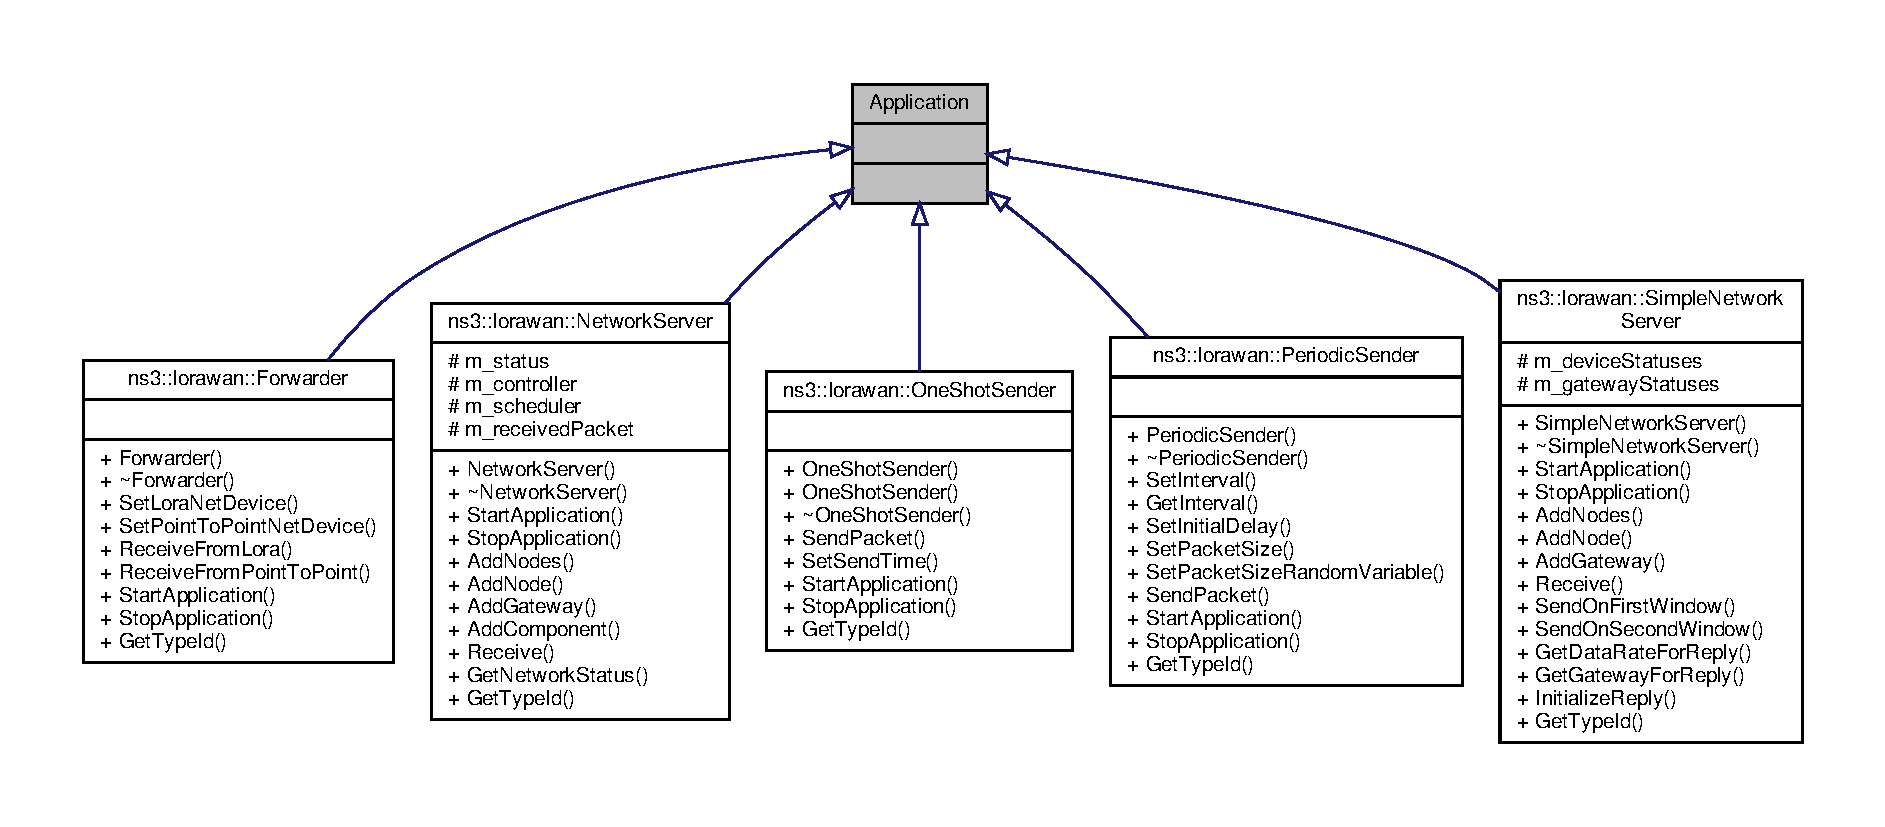
\includegraphics[width=350pt]{classApplication__inherit__graph}
\end{center}
\end{figure}


Collaboration diagram for Application\+:
\nopagebreak
\begin{figure}[H]
\begin{center}
\leavevmode
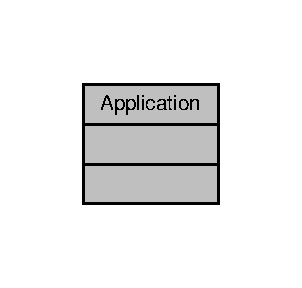
\includegraphics[width=145pt]{classApplication__coll__graph}
\end{center}
\end{figure}


The documentation for this class was generated from the following file\+:\begin{DoxyCompactItemize}
\item 
one-\/shot-\/sender.\+h\end{DoxyCompactItemize}

\hypertarget{classns3_1_1lorawan_1_1BuildingPenetrationLoss}{}\section{ns3\+:\+:lorawan\+:\+:Building\+Penetration\+Loss Class Reference}
\label{classns3_1_1lorawan_1_1BuildingPenetrationLoss}\index{ns3\+::lorawan\+::\+Building\+Penetration\+Loss@{ns3\+::lorawan\+::\+Building\+Penetration\+Loss}}


{\ttfamily \#include $<$building-\/penetration-\/loss.\+h$>$}



Inheritance diagram for ns3\+:\+:lorawan\+:\+:Building\+Penetration\+Loss\+:
\nopagebreak
\begin{figure}[H]
\begin{center}
\leavevmode
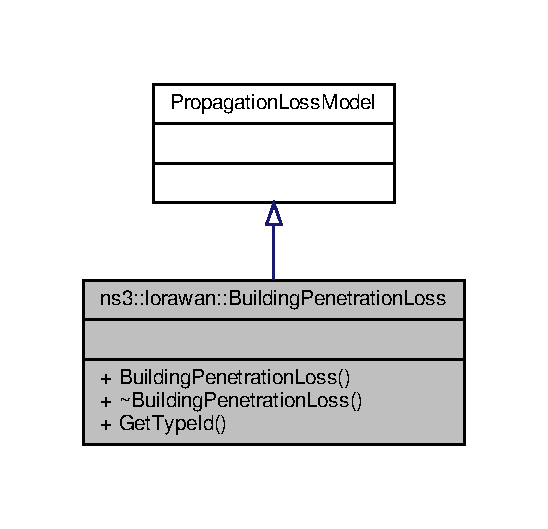
\includegraphics[width=263pt]{classns3_1_1lorawan_1_1BuildingPenetrationLoss__inherit__graph}
\end{center}
\end{figure}


Collaboration diagram for ns3\+:\+:lorawan\+:\+:Building\+Penetration\+Loss\+:
\nopagebreak
\begin{figure}[H]
\begin{center}
\leavevmode
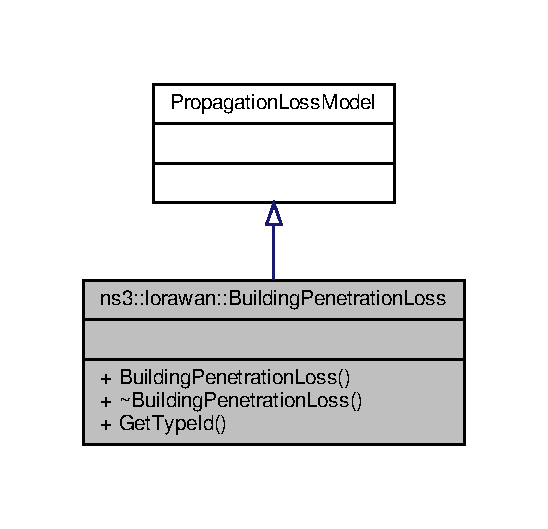
\includegraphics[width=263pt]{classns3_1_1lorawan_1_1BuildingPenetrationLoss__coll__graph}
\end{center}
\end{figure}
\subsection*{Static Public Member Functions}
\begin{DoxyCompactItemize}
\item 
\mbox{\Hypertarget{classns3_1_1lorawan_1_1BuildingPenetrationLoss_ad3ffa20fecb2e17a367f95b965c8c6a3}\label{classns3_1_1lorawan_1_1BuildingPenetrationLoss_ad3ffa20fecb2e17a367f95b965c8c6a3}} 
static Type\+Id {\bfseries Get\+Type\+Id} (void)
\end{DoxyCompactItemize}


\subsection{Detailed Description}
A class implementing the TR 45.\+820 model for building losses 

The documentation for this class was generated from the following files\+:\begin{DoxyCompactItemize}
\item 
building-\/penetration-\/loss.\+h\item 
building-\/penetration-\/loss.\+cc\end{DoxyCompactItemize}

\hypertarget{classChannel}{}\section{Channel Class Reference}
\label{classChannel}\index{Channel@{Channel}}


Inheritance diagram for Channel\+:
\nopagebreak
\begin{figure}[H]
\begin{center}
\leavevmode
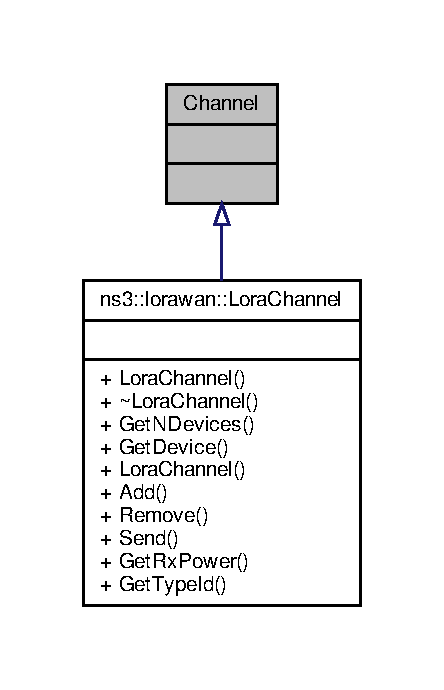
\includegraphics[width=213pt]{classChannel__inherit__graph}
\end{center}
\end{figure}


Collaboration diagram for Channel\+:
\nopagebreak
\begin{figure}[H]
\begin{center}
\leavevmode
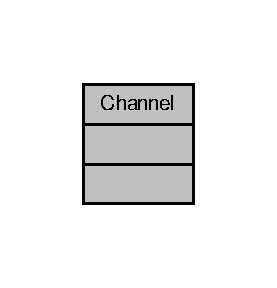
\includegraphics[width=133pt]{classChannel__coll__graph}
\end{center}
\end{figure}


The documentation for this class was generated from the following file\+:\begin{DoxyCompactItemize}
\item 
lora-\/channel.\+h\end{DoxyCompactItemize}

\hypertarget{classns3_1_1lorawan_1_1ConfirmedMessagesComponent}{}\section{ns3\+:\+:lorawan\+:\+:Confirmed\+Messages\+Component Class Reference}
\label{classns3_1_1lorawan_1_1ConfirmedMessagesComponent}\index{ns3\+::lorawan\+::\+Confirmed\+Messages\+Component@{ns3\+::lorawan\+::\+Confirmed\+Messages\+Component}}


Inheritance diagram for ns3\+:\+:lorawan\+:\+:Confirmed\+Messages\+Component\+:
\nopagebreak
\begin{figure}[H]
\begin{center}
\leavevmode
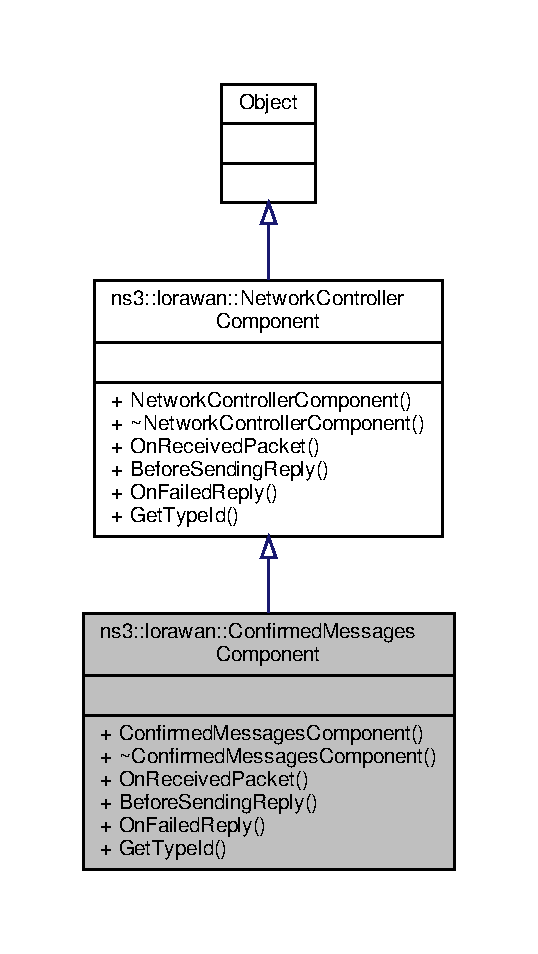
\includegraphics[width=258pt]{classns3_1_1lorawan_1_1ConfirmedMessagesComponent__inherit__graph}
\end{center}
\end{figure}


Collaboration diagram for ns3\+:\+:lorawan\+:\+:Confirmed\+Messages\+Component\+:
\nopagebreak
\begin{figure}[H]
\begin{center}
\leavevmode
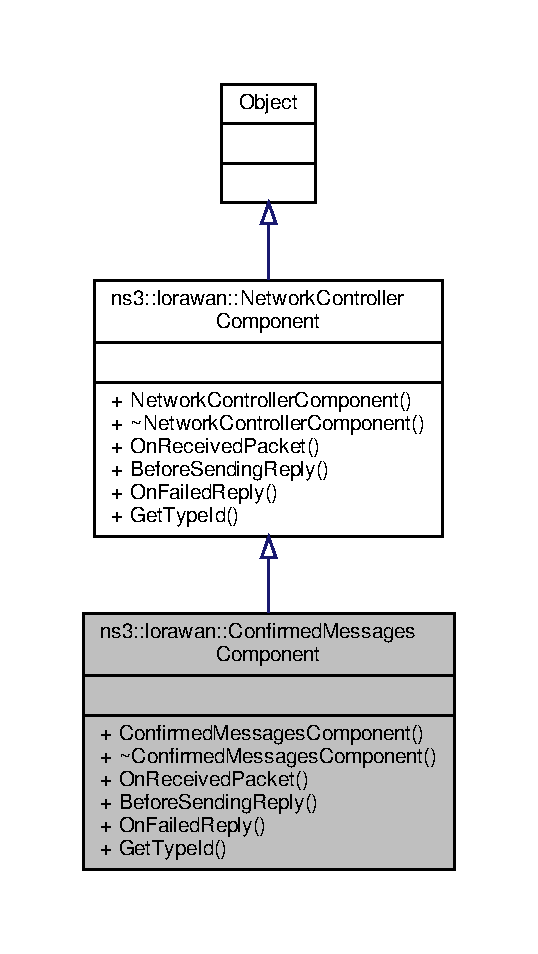
\includegraphics[width=258pt]{classns3_1_1lorawan_1_1ConfirmedMessagesComponent__coll__graph}
\end{center}
\end{figure}
\subsection*{Public Member Functions}
\begin{DoxyCompactItemize}
\item 
void \hyperlink{classns3_1_1lorawan_1_1ConfirmedMessagesComponent_a0e58f518722ae87373d6a33e7523e8b1}{On\+Received\+Packet} (Ptr$<$ const Packet $>$ packet, Ptr$<$ \hyperlink{classns3_1_1lorawan_1_1EndDeviceStatus}{End\+Device\+Status} $>$ status, Ptr$<$ \hyperlink{classns3_1_1lorawan_1_1NetworkStatus}{Network\+Status} $>$ network\+Status)
\item 
\mbox{\Hypertarget{classns3_1_1lorawan_1_1ConfirmedMessagesComponent_a49e51698752d21f29d26ea1f8d01ecbf}\label{classns3_1_1lorawan_1_1ConfirmedMessagesComponent_a49e51698752d21f29d26ea1f8d01ecbf}} 
void {\bfseries Before\+Sending\+Reply} (Ptr$<$ \hyperlink{classns3_1_1lorawan_1_1EndDeviceStatus}{End\+Device\+Status} $>$ status, Ptr$<$ \hyperlink{classns3_1_1lorawan_1_1NetworkStatus}{Network\+Status} $>$ network\+Status)
\item 
void \hyperlink{classns3_1_1lorawan_1_1ConfirmedMessagesComponent_ae048f3d5aff4da319d113c213701ef73}{On\+Failed\+Reply} (Ptr$<$ \hyperlink{classns3_1_1lorawan_1_1EndDeviceStatus}{End\+Device\+Status} $>$ status, Ptr$<$ \hyperlink{classns3_1_1lorawan_1_1NetworkStatus}{Network\+Status} $>$ network\+Status)
\end{DoxyCompactItemize}
\subsection*{Static Public Member Functions}
\begin{DoxyCompactItemize}
\item 
\mbox{\Hypertarget{classns3_1_1lorawan_1_1ConfirmedMessagesComponent_aceef26b9e73d26f22262101e0caf0476}\label{classns3_1_1lorawan_1_1ConfirmedMessagesComponent_aceef26b9e73d26f22262101e0caf0476}} 
static Type\+Id {\bfseries Get\+Type\+Id} (void)
\end{DoxyCompactItemize}


\subsection{Member Function Documentation}
\mbox{\Hypertarget{classns3_1_1lorawan_1_1ConfirmedMessagesComponent_ae048f3d5aff4da319d113c213701ef73}\label{classns3_1_1lorawan_1_1ConfirmedMessagesComponent_ae048f3d5aff4da319d113c213701ef73}} 
\index{ns3\+::lorawan\+::\+Confirmed\+Messages\+Component@{ns3\+::lorawan\+::\+Confirmed\+Messages\+Component}!On\+Failed\+Reply@{On\+Failed\+Reply}}
\index{On\+Failed\+Reply@{On\+Failed\+Reply}!ns3\+::lorawan\+::\+Confirmed\+Messages\+Component@{ns3\+::lorawan\+::\+Confirmed\+Messages\+Component}}
\subsubsection{\texorpdfstring{On\+Failed\+Reply()}{OnFailedReply()}}
{\footnotesize\ttfamily void ns3\+::lorawan\+::\+Confirmed\+Messages\+Component\+::\+On\+Failed\+Reply (\begin{DoxyParamCaption}\item[{Ptr$<$ \hyperlink{classns3_1_1lorawan_1_1EndDeviceStatus}{End\+Device\+Status} $>$}]{status,  }\item[{Ptr$<$ \hyperlink{classns3_1_1lorawan_1_1NetworkStatus}{Network\+Status} $>$}]{network\+Status }\end{DoxyParamCaption})\hspace{0.3cm}{\ttfamily [virtual]}}

Method that is called when a packet cannot be sent in the downlink.


\begin{DoxyParams}{Parameters}
{\em status} & The \hyperlink{classns3_1_1lorawan_1_1EndDeviceStatus}{End\+Device\+Status} of the device to which it was impossible to send a reply. \\
\hline
{\em network\+Status} & A pointer to the \hyperlink{classns3_1_1lorawan_1_1NetworkStatus}{Network\+Status} object \\
\hline
\end{DoxyParams}


Implements \hyperlink{classns3_1_1lorawan_1_1NetworkControllerComponent_aaff757f6ece10a8ef24564006c137d72}{ns3\+::lorawan\+::\+Network\+Controller\+Component}.

\mbox{\Hypertarget{classns3_1_1lorawan_1_1ConfirmedMessagesComponent_a0e58f518722ae87373d6a33e7523e8b1}\label{classns3_1_1lorawan_1_1ConfirmedMessagesComponent_a0e58f518722ae87373d6a33e7523e8b1}} 
\index{ns3\+::lorawan\+::\+Confirmed\+Messages\+Component@{ns3\+::lorawan\+::\+Confirmed\+Messages\+Component}!On\+Received\+Packet@{On\+Received\+Packet}}
\index{On\+Received\+Packet@{On\+Received\+Packet}!ns3\+::lorawan\+::\+Confirmed\+Messages\+Component@{ns3\+::lorawan\+::\+Confirmed\+Messages\+Component}}
\subsubsection{\texorpdfstring{On\+Received\+Packet()}{OnReceivedPacket()}}
{\footnotesize\ttfamily void ns3\+::lorawan\+::\+Confirmed\+Messages\+Component\+::\+On\+Received\+Packet (\begin{DoxyParamCaption}\item[{Ptr$<$ const Packet $>$}]{packet,  }\item[{Ptr$<$ \hyperlink{classns3_1_1lorawan_1_1EndDeviceStatus}{End\+Device\+Status} $>$}]{status,  }\item[{Ptr$<$ \hyperlink{classns3_1_1lorawan_1_1NetworkStatus}{Network\+Status} $>$}]{network\+Status }\end{DoxyParamCaption})\hspace{0.3cm}{\ttfamily [virtual]}}

This method checks whether the received packet requires an acknowledgment and sets up the appropriate reply in case it does.


\begin{DoxyParams}{Parameters}
{\em packet} & The newly received packet \\
\hline
{\em network\+Status} & A pointer to the \hyperlink{classns3_1_1lorawan_1_1NetworkStatus}{Network\+Status} object \\
\hline
\end{DoxyParams}


Implements \hyperlink{classns3_1_1lorawan_1_1NetworkControllerComponent_a965fb667c3e88703e8cdbcbcd057db6f}{ns3\+::lorawan\+::\+Network\+Controller\+Component}.



The documentation for this class was generated from the following files\+:\begin{DoxyCompactItemize}
\item 
network-\/controller-\/components.\+h\item 
network-\/controller-\/components.\+cc\end{DoxyCompactItemize}

\hypertarget{classns3_1_1lorawan_1_1ConstantLoraTxCurrentModel}{}\section{ns3\+:\+:lorawan\+:\+:Constant\+Lora\+Tx\+Current\+Model Class Reference}
\label{classns3_1_1lorawan_1_1ConstantLoraTxCurrentModel}\index{ns3\+::lorawan\+::\+Constant\+Lora\+Tx\+Current\+Model@{ns3\+::lorawan\+::\+Constant\+Lora\+Tx\+Current\+Model}}


Inheritance diagram for ns3\+:\+:lorawan\+:\+:Constant\+Lora\+Tx\+Current\+Model\+:
\nopagebreak
\begin{figure}[H]
\begin{center}
\leavevmode
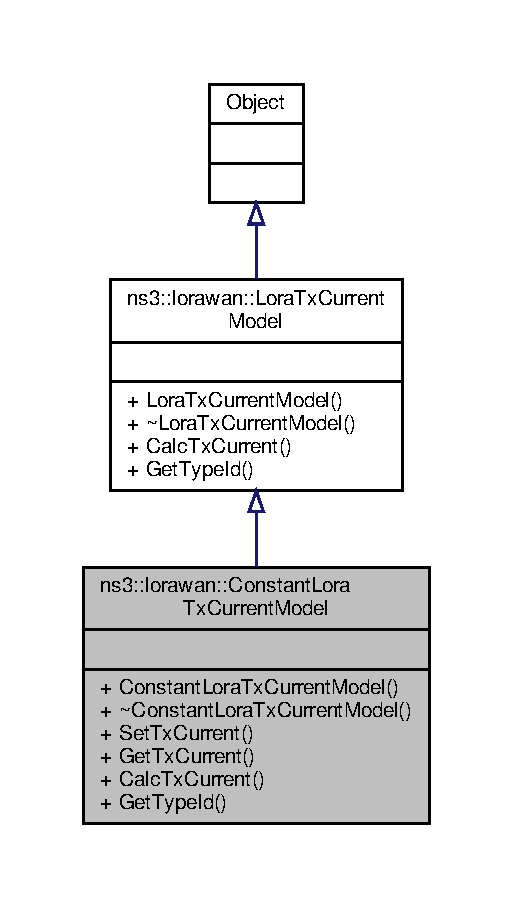
\includegraphics[width=246pt]{classns3_1_1lorawan_1_1ConstantLoraTxCurrentModel__inherit__graph}
\end{center}
\end{figure}


Collaboration diagram for ns3\+:\+:lorawan\+:\+:Constant\+Lora\+Tx\+Current\+Model\+:
\nopagebreak
\begin{figure}[H]
\begin{center}
\leavevmode
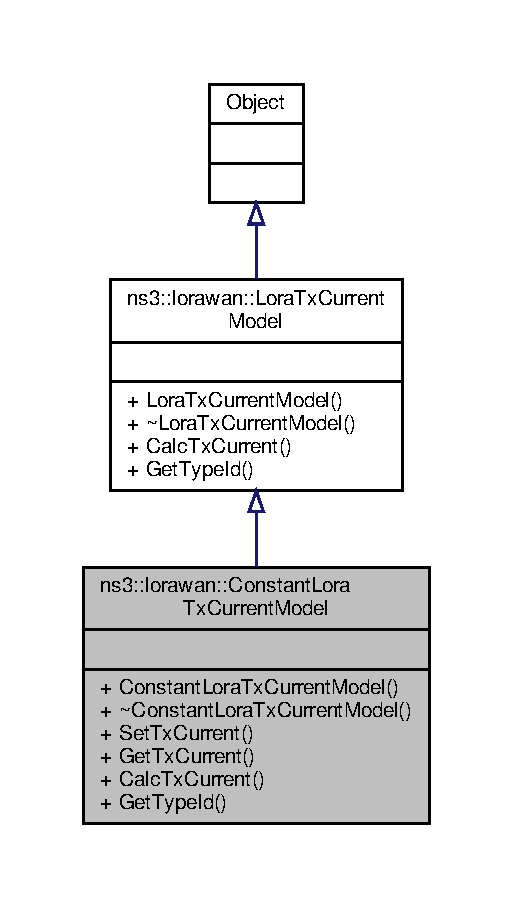
\includegraphics[width=246pt]{classns3_1_1lorawan_1_1ConstantLoraTxCurrentModel__coll__graph}
\end{center}
\end{figure}
\subsection*{Public Member Functions}
\begin{DoxyCompactItemize}
\item 
void \hyperlink{classns3_1_1lorawan_1_1ConstantLoraTxCurrentModel_a3c1a59240065eb000df03cbd34b020da}{Set\+Tx\+Current} (double tx\+Current)
\item 
double \hyperlink{classns3_1_1lorawan_1_1ConstantLoraTxCurrentModel_a0c26b75e61ba7f9c4c6773a2e9741215}{Get\+Tx\+Current} (void) const
\item 
double \hyperlink{classns3_1_1lorawan_1_1ConstantLoraTxCurrentModel_afd0b31a415eae9f95dd4464612925dad}{Calc\+Tx\+Current} (double tx\+Power\+Dbm) const
\end{DoxyCompactItemize}
\subsection*{Static Public Member Functions}
\begin{DoxyCompactItemize}
\item 
static Type\+Id \hyperlink{classns3_1_1lorawan_1_1ConstantLoraTxCurrentModel_aec6efa40cd05eaeecb90b111160e8630}{Get\+Type\+Id} (void)
\begin{DoxyCompactList}\small\item\em Get the type ID. \end{DoxyCompactList}\end{DoxyCompactItemize}


\subsection{Member Function Documentation}
\mbox{\Hypertarget{classns3_1_1lorawan_1_1ConstantLoraTxCurrentModel_afd0b31a415eae9f95dd4464612925dad}\label{classns3_1_1lorawan_1_1ConstantLoraTxCurrentModel_afd0b31a415eae9f95dd4464612925dad}} 
\index{ns3\+::lorawan\+::\+Constant\+Lora\+Tx\+Current\+Model@{ns3\+::lorawan\+::\+Constant\+Lora\+Tx\+Current\+Model}!Calc\+Tx\+Current@{Calc\+Tx\+Current}}
\index{Calc\+Tx\+Current@{Calc\+Tx\+Current}!ns3\+::lorawan\+::\+Constant\+Lora\+Tx\+Current\+Model@{ns3\+::lorawan\+::\+Constant\+Lora\+Tx\+Current\+Model}}
\subsubsection{\texorpdfstring{Calc\+Tx\+Current()}{CalcTxCurrent()}}
{\footnotesize\ttfamily double ns3\+::lorawan\+::\+Constant\+Lora\+Tx\+Current\+Model\+::\+Calc\+Tx\+Current (\begin{DoxyParamCaption}\item[{double}]{tx\+Power\+Dbm }\end{DoxyParamCaption}) const\hspace{0.3cm}{\ttfamily [virtual]}}

Get the current for transmission at this power.


\begin{DoxyParams}{Parameters}
{\em tx\+Power\+Dbm} & The nominal tx power in d\+Bm \\
\hline
\end{DoxyParams}
\begin{DoxyReturn}{Returns}
The transmit current (in Ampere) 
\end{DoxyReturn}


Implements \hyperlink{classns3_1_1lorawan_1_1LoraTxCurrentModel_ad4143a40cb10d4cbd4bf838e006780c7}{ns3\+::lorawan\+::\+Lora\+Tx\+Current\+Model}.

\mbox{\Hypertarget{classns3_1_1lorawan_1_1ConstantLoraTxCurrentModel_a0c26b75e61ba7f9c4c6773a2e9741215}\label{classns3_1_1lorawan_1_1ConstantLoraTxCurrentModel_a0c26b75e61ba7f9c4c6773a2e9741215}} 
\index{ns3\+::lorawan\+::\+Constant\+Lora\+Tx\+Current\+Model@{ns3\+::lorawan\+::\+Constant\+Lora\+Tx\+Current\+Model}!Get\+Tx\+Current@{Get\+Tx\+Current}}
\index{Get\+Tx\+Current@{Get\+Tx\+Current}!ns3\+::lorawan\+::\+Constant\+Lora\+Tx\+Current\+Model@{ns3\+::lorawan\+::\+Constant\+Lora\+Tx\+Current\+Model}}
\subsubsection{\texorpdfstring{Get\+Tx\+Current()}{GetTxCurrent()}}
{\footnotesize\ttfamily double ns3\+::lorawan\+::\+Constant\+Lora\+Tx\+Current\+Model\+::\+Get\+Tx\+Current (\begin{DoxyParamCaption}\item[{void}]{ }\end{DoxyParamCaption}) const}

\begin{DoxyReturn}{Returns}
the current in the TX state. 
\end{DoxyReturn}
\mbox{\Hypertarget{classns3_1_1lorawan_1_1ConstantLoraTxCurrentModel_aec6efa40cd05eaeecb90b111160e8630}\label{classns3_1_1lorawan_1_1ConstantLoraTxCurrentModel_aec6efa40cd05eaeecb90b111160e8630}} 
\index{ns3\+::lorawan\+::\+Constant\+Lora\+Tx\+Current\+Model@{ns3\+::lorawan\+::\+Constant\+Lora\+Tx\+Current\+Model}!Get\+Type\+Id@{Get\+Type\+Id}}
\index{Get\+Type\+Id@{Get\+Type\+Id}!ns3\+::lorawan\+::\+Constant\+Lora\+Tx\+Current\+Model@{ns3\+::lorawan\+::\+Constant\+Lora\+Tx\+Current\+Model}}
\subsubsection{\texorpdfstring{Get\+Type\+Id()}{GetTypeId()}}
{\footnotesize\ttfamily Type\+Id ns3\+::lorawan\+::\+Constant\+Lora\+Tx\+Current\+Model\+::\+Get\+Type\+Id (\begin{DoxyParamCaption}\item[{void}]{ }\end{DoxyParamCaption})\hspace{0.3cm}{\ttfamily [static]}}



Get the type ID. 

\begin{DoxyReturn}{Returns}
the object Type\+Id 
\end{DoxyReturn}
\mbox{\Hypertarget{classns3_1_1lorawan_1_1ConstantLoraTxCurrentModel_a3c1a59240065eb000df03cbd34b020da}\label{classns3_1_1lorawan_1_1ConstantLoraTxCurrentModel_a3c1a59240065eb000df03cbd34b020da}} 
\index{ns3\+::lorawan\+::\+Constant\+Lora\+Tx\+Current\+Model@{ns3\+::lorawan\+::\+Constant\+Lora\+Tx\+Current\+Model}!Set\+Tx\+Current@{Set\+Tx\+Current}}
\index{Set\+Tx\+Current@{Set\+Tx\+Current}!ns3\+::lorawan\+::\+Constant\+Lora\+Tx\+Current\+Model@{ns3\+::lorawan\+::\+Constant\+Lora\+Tx\+Current\+Model}}
\subsubsection{\texorpdfstring{Set\+Tx\+Current()}{SetTxCurrent()}}
{\footnotesize\ttfamily void ns3\+::lorawan\+::\+Constant\+Lora\+Tx\+Current\+Model\+::\+Set\+Tx\+Current (\begin{DoxyParamCaption}\item[{double}]{tx\+Current }\end{DoxyParamCaption})}


\begin{DoxyParams}{Parameters}
{\em tx\+Current} & (Ampere)\\
\hline
\end{DoxyParams}
Set the current in the TX state. 

The documentation for this class was generated from the following files\+:\begin{DoxyCompactItemize}
\item 
lora-\/tx-\/current-\/model.\+h\item 
lora-\/tx-\/current-\/model.\+cc\end{DoxyCompactItemize}

\hypertarget{classns3_1_1lorawan_1_1CorrelatedShadowingPropagationLossModel}{}\section{ns3\+:\+:lorawan\+:\+:Correlated\+Shadowing\+Propagation\+Loss\+Model Class Reference}
\label{classns3_1_1lorawan_1_1CorrelatedShadowingPropagationLossModel}\index{ns3\+::lorawan\+::\+Correlated\+Shadowing\+Propagation\+Loss\+Model@{ns3\+::lorawan\+::\+Correlated\+Shadowing\+Propagation\+Loss\+Model}}


Inheritance diagram for ns3\+:\+:lorawan\+:\+:Correlated\+Shadowing\+Propagation\+Loss\+Model\+:
\nopagebreak
\begin{figure}[H]
\begin{center}
\leavevmode
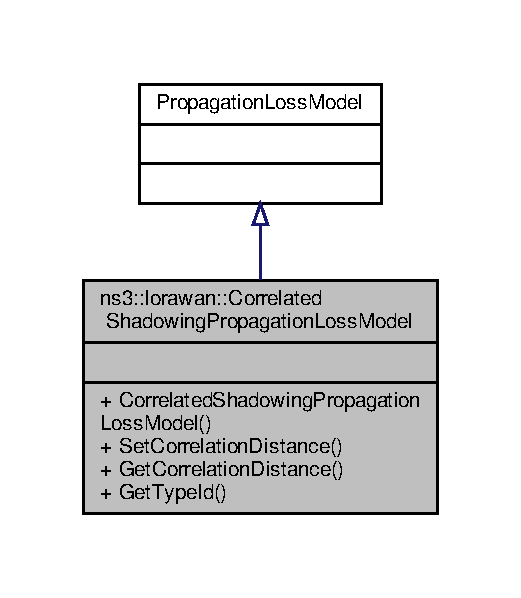
\includegraphics[width=250pt]{classns3_1_1lorawan_1_1CorrelatedShadowingPropagationLossModel__inherit__graph}
\end{center}
\end{figure}


Collaboration diagram for ns3\+:\+:lorawan\+:\+:Correlated\+Shadowing\+Propagation\+Loss\+Model\+:
\nopagebreak
\begin{figure}[H]
\begin{center}
\leavevmode
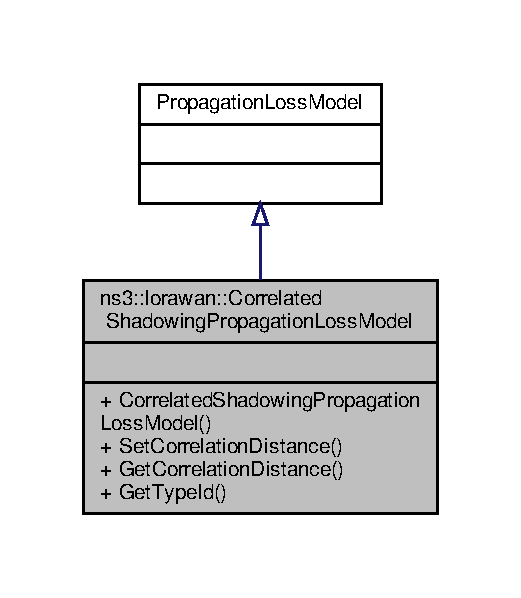
\includegraphics[width=250pt]{classns3_1_1lorawan_1_1CorrelatedShadowingPropagationLossModel__coll__graph}
\end{center}
\end{figure}
\subsection*{Classes}
\begin{DoxyCompactItemize}
\item 
class \hyperlink{classns3_1_1lorawan_1_1CorrelatedShadowingPropagationLossModel_1_1Position}{Position}
\item 
class \hyperlink{classns3_1_1lorawan_1_1CorrelatedShadowingPropagationLossModel_1_1ShadowingMap}{Shadowing\+Map}
\end{DoxyCompactItemize}
\subsection*{Public Member Functions}
\begin{DoxyCompactItemize}
\item 
\hyperlink{classns3_1_1lorawan_1_1CorrelatedShadowingPropagationLossModel_a19673646a3b2169c15cd9b751d1d9d96}{Correlated\+Shadowing\+Propagation\+Loss\+Model} ()
\item 
void \hyperlink{classns3_1_1lorawan_1_1CorrelatedShadowingPropagationLossModel_a1553b2a1935dc8e59d3326bee538736c}{Set\+Correlation\+Distance} (double distance)
\item 
double \hyperlink{classns3_1_1lorawan_1_1CorrelatedShadowingPropagationLossModel_a0eef282d061a1acaf38be072da24faa6}{Get\+Correlation\+Distance} (void)
\end{DoxyCompactItemize}
\subsection*{Static Public Member Functions}
\begin{DoxyCompactItemize}
\item 
\mbox{\Hypertarget{classns3_1_1lorawan_1_1CorrelatedShadowingPropagationLossModel_ab5cc8de84edced7bd9ed701cd341a8a9}\label{classns3_1_1lorawan_1_1CorrelatedShadowingPropagationLossModel_ab5cc8de84edced7bd9ed701cd341a8a9}} 
static Type\+Id {\bfseries Get\+Type\+Id} (void)
\end{DoxyCompactItemize}


\subsection{Constructor \& Destructor Documentation}
\mbox{\Hypertarget{classns3_1_1lorawan_1_1CorrelatedShadowingPropagationLossModel_a19673646a3b2169c15cd9b751d1d9d96}\label{classns3_1_1lorawan_1_1CorrelatedShadowingPropagationLossModel_a19673646a3b2169c15cd9b751d1d9d96}} 
\index{ns3\+::lorawan\+::\+Correlated\+Shadowing\+Propagation\+Loss\+Model@{ns3\+::lorawan\+::\+Correlated\+Shadowing\+Propagation\+Loss\+Model}!Correlated\+Shadowing\+Propagation\+Loss\+Model@{Correlated\+Shadowing\+Propagation\+Loss\+Model}}
\index{Correlated\+Shadowing\+Propagation\+Loss\+Model@{Correlated\+Shadowing\+Propagation\+Loss\+Model}!ns3\+::lorawan\+::\+Correlated\+Shadowing\+Propagation\+Loss\+Model@{ns3\+::lorawan\+::\+Correlated\+Shadowing\+Propagation\+Loss\+Model}}
\subsubsection{\texorpdfstring{Correlated\+Shadowing\+Propagation\+Loss\+Model()}{CorrelatedShadowingPropagationLossModel()}}
{\footnotesize\ttfamily ns3\+::lorawan\+::\+Correlated\+Shadowing\+Propagation\+Loss\+Model\+::\+Correlated\+Shadowing\+Propagation\+Loss\+Model (\begin{DoxyParamCaption}{ }\end{DoxyParamCaption})}

Constructor. 

\subsection{Member Function Documentation}
\mbox{\Hypertarget{classns3_1_1lorawan_1_1CorrelatedShadowingPropagationLossModel_a0eef282d061a1acaf38be072da24faa6}\label{classns3_1_1lorawan_1_1CorrelatedShadowingPropagationLossModel_a0eef282d061a1acaf38be072da24faa6}} 
\index{ns3\+::lorawan\+::\+Correlated\+Shadowing\+Propagation\+Loss\+Model@{ns3\+::lorawan\+::\+Correlated\+Shadowing\+Propagation\+Loss\+Model}!Get\+Correlation\+Distance@{Get\+Correlation\+Distance}}
\index{Get\+Correlation\+Distance@{Get\+Correlation\+Distance}!ns3\+::lorawan\+::\+Correlated\+Shadowing\+Propagation\+Loss\+Model@{ns3\+::lorawan\+::\+Correlated\+Shadowing\+Propagation\+Loss\+Model}}
\subsubsection{\texorpdfstring{Get\+Correlation\+Distance()}{GetCorrelationDistance()}}
{\footnotesize\ttfamily double ns3\+::lorawan\+::\+Correlated\+Shadowing\+Propagation\+Loss\+Model\+::\+Get\+Correlation\+Distance (\begin{DoxyParamCaption}\item[{void}]{ }\end{DoxyParamCaption})}

Get the correlation distance that is currently being used. \mbox{\Hypertarget{classns3_1_1lorawan_1_1CorrelatedShadowingPropagationLossModel_a1553b2a1935dc8e59d3326bee538736c}\label{classns3_1_1lorawan_1_1CorrelatedShadowingPropagationLossModel_a1553b2a1935dc8e59d3326bee538736c}} 
\index{ns3\+::lorawan\+::\+Correlated\+Shadowing\+Propagation\+Loss\+Model@{ns3\+::lorawan\+::\+Correlated\+Shadowing\+Propagation\+Loss\+Model}!Set\+Correlation\+Distance@{Set\+Correlation\+Distance}}
\index{Set\+Correlation\+Distance@{Set\+Correlation\+Distance}!ns3\+::lorawan\+::\+Correlated\+Shadowing\+Propagation\+Loss\+Model@{ns3\+::lorawan\+::\+Correlated\+Shadowing\+Propagation\+Loss\+Model}}
\subsubsection{\texorpdfstring{Set\+Correlation\+Distance()}{SetCorrelationDistance()}}
{\footnotesize\ttfamily void ns3\+::lorawan\+::\+Correlated\+Shadowing\+Propagation\+Loss\+Model\+::\+Set\+Correlation\+Distance (\begin{DoxyParamCaption}\item[{double}]{distance }\end{DoxyParamCaption})}

Set the correlation distance for newly created \hyperlink{classns3_1_1lorawan_1_1CorrelatedShadowingPropagationLossModel_1_1ShadowingMap}{Shadowing\+Map} instances 

The documentation for this class was generated from the following files\+:\begin{DoxyCompactItemize}
\item 
correlated-\/shadowing-\/propagation-\/loss-\/model.\+h\item 
correlated-\/shadowing-\/propagation-\/loss-\/model.\+cc\end{DoxyCompactItemize}

\hypertarget{classDeviceEnergyModel}{}\section{Device\+Energy\+Model Class Reference}
\label{classDeviceEnergyModel}\index{Device\+Energy\+Model@{Device\+Energy\+Model}}


Inheritance diagram for Device\+Energy\+Model\+:
\nopagebreak
\begin{figure}[H]
\begin{center}
\leavevmode
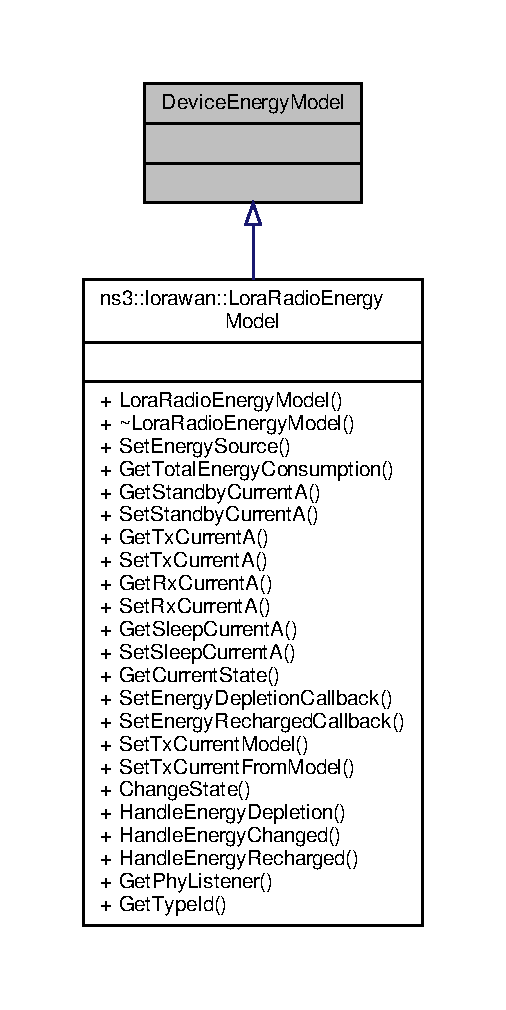
\includegraphics[width=243pt]{classDeviceEnergyModel__inherit__graph}
\end{center}
\end{figure}


Collaboration diagram for Device\+Energy\+Model\+:
\nopagebreak
\begin{figure}[H]
\begin{center}
\leavevmode
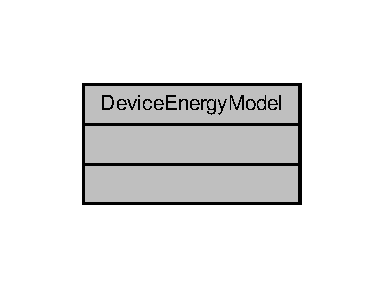
\includegraphics[width=184pt]{classDeviceEnergyModel__coll__graph}
\end{center}
\end{figure}


The documentation for this class was generated from the following file\+:\begin{DoxyCompactItemize}
\item 
lora-\/radio-\/energy-\/model.\+h\end{DoxyCompactItemize}

\hypertarget{classns3_1_1lorawan_1_1DeviceStatus}{}\section{ns3\+:\+:lorawan\+:\+:Device\+Status Class Reference}
\label{classns3_1_1lorawan_1_1DeviceStatus}\index{ns3\+::lorawan\+::\+Device\+Status@{ns3\+::lorawan\+::\+Device\+Status}}


{\ttfamily \#include $<$device-\/status.\+h$>$}



Collaboration diagram for ns3\+:\+:lorawan\+:\+:Device\+Status\+:
\nopagebreak
\begin{figure}[H]
\begin{center}
\leavevmode
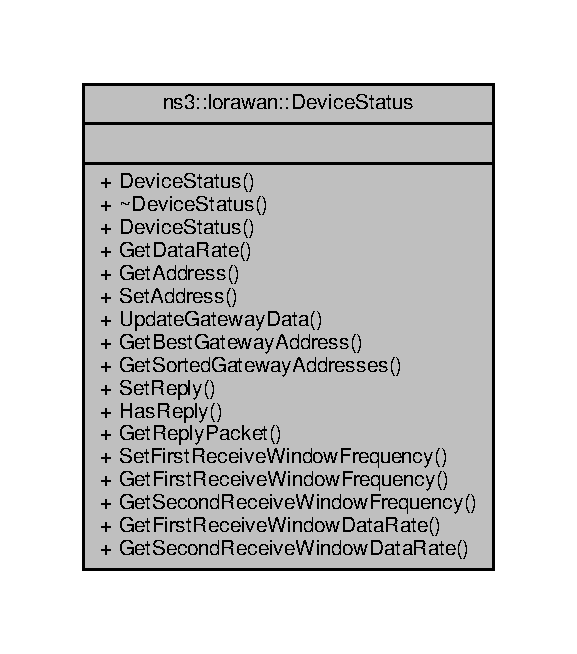
\includegraphics[width=277pt]{classns3_1_1lorawan_1_1DeviceStatus__coll__graph}
\end{center}
\end{figure}
\subsection*{Classes}
\begin{DoxyCompactItemize}
\item 
struct \hyperlink{structns3_1_1lorawan_1_1DeviceStatus_1_1Reply}{Reply}
\end{DoxyCompactItemize}
\subsection*{Public Member Functions}
\begin{DoxyCompactItemize}
\item 
\mbox{\Hypertarget{classns3_1_1lorawan_1_1DeviceStatus_ac00447539b1da7b1c4aeb7479b5d48ff}\label{classns3_1_1lorawan_1_1DeviceStatus_ac00447539b1da7b1c4aeb7479b5d48ff}} 
{\bfseries Device\+Status} (Ptr$<$ \hyperlink{classns3_1_1lorawan_1_1EndDeviceLoraMac}{End\+Device\+Lora\+Mac} $>$ end\+Device\+Mac)
\item 
uint8\+\_\+t \hyperlink{classns3_1_1lorawan_1_1DeviceStatus_af0d05320ecdc282c13597c101076c605}{Get\+Data\+Rate} ()
\item 
\hyperlink{classns3_1_1lorawan_1_1LoraDeviceAddress}{Lora\+Device\+Address} \hyperlink{classns3_1_1lorawan_1_1DeviceStatus_ad1ff55d93bc1347ac860a921d590053e}{Get\+Address} ()
\item 
void \hyperlink{classns3_1_1lorawan_1_1DeviceStatus_a690f9059f8cc8b6ce516da4d670f4b94}{Set\+Address} (\hyperlink{classns3_1_1lorawan_1_1LoraDeviceAddress}{Lora\+Device\+Address} address)
\item 
void \hyperlink{classns3_1_1lorawan_1_1DeviceStatus_a76581259b5b053500387dc3e9b73094b}{Update\+Gateway\+Data} (Address gw\+Address, double rcv\+Power)
\item 
Address \hyperlink{classns3_1_1lorawan_1_1DeviceStatus_a339650bdf62a9c13d458f4276222e740}{Get\+Best\+Gateway\+Address} (void)
\item 
std\+::list$<$ Address $>$ \hyperlink{classns3_1_1lorawan_1_1DeviceStatus_a6174dfca1f330b02f833683117acecdb}{Get\+Sorted\+Gateway\+Addresses} (void)
\item 
void \hyperlink{classns3_1_1lorawan_1_1DeviceStatus_a10001b2464375197ac57462323ef2766}{Set\+Reply} (struct \hyperlink{structns3_1_1lorawan_1_1DeviceStatus_1_1Reply}{Reply} reply)
\item 
bool \hyperlink{classns3_1_1lorawan_1_1DeviceStatus_a1a713e0523cef431cd3194aa27bd6f57}{Has\+Reply} (void)
\item 
Ptr$<$ Packet $>$ \hyperlink{classns3_1_1lorawan_1_1DeviceStatus_ad83a579eab32d419aeb0409d959a8ff0}{Get\+Reply\+Packet} (void)
\item 
void \hyperlink{classns3_1_1lorawan_1_1DeviceStatus_a27f4dfe68d8361e4835c50865aaf7325}{Set\+First\+Receive\+Window\+Frequency} (double frequency)
\item 
double \hyperlink{classns3_1_1lorawan_1_1DeviceStatus_ab83d8a40859427f84e56f6536d1337de}{Get\+First\+Receive\+Window\+Frequency} (void)
\item 
double \hyperlink{classns3_1_1lorawan_1_1DeviceStatus_a3b908979aaebd791d3c54196fcf938f1}{Get\+Second\+Receive\+Window\+Frequency} (void)
\item 
uint8\+\_\+t \hyperlink{classns3_1_1lorawan_1_1DeviceStatus_a4645606cdd1fd2f4c94d1f8ec919f49f}{Get\+First\+Receive\+Window\+Data\+Rate} (void)
\item 
uint8\+\_\+t \hyperlink{classns3_1_1lorawan_1_1DeviceStatus_a65e9a5079d08a3e85db3c9ecc5c2177c}{Get\+Second\+Receive\+Window\+Data\+Rate} (void)
\end{DoxyCompactItemize}


\subsection{Detailed Description}
This class represents the Network Server\textquotesingle{}s knowledge about an End Device in the Lo\+Ra\+W\+AN network it is administering.

The Network Server contains a list of instances of this class, once for each device in the network. This class holds the reply packet that the network server will send to this device at the first available receive window. Furthermore, this class is used to keep track of all gateways that are able to receive the device\textquotesingle{}s packets. On new packet arrivals at the Network Server, the Update\+Gateway\+Data method is called to update the m\+\_\+gateways map, that associates a Gateway\textquotesingle{}s Point\+To\+Point\+Net\+Device address to the power it received this ED\textquotesingle{}s last packet. This information is then used in the Get\+Sorted\+Gateway\+Addresses method to return a list of the preferred gateways through which to reply to this device. 

\subsection{Member Function Documentation}
\mbox{\Hypertarget{classns3_1_1lorawan_1_1DeviceStatus_ad1ff55d93bc1347ac860a921d590053e}\label{classns3_1_1lorawan_1_1DeviceStatus_ad1ff55d93bc1347ac860a921d590053e}} 
\index{ns3\+::lorawan\+::\+Device\+Status@{ns3\+::lorawan\+::\+Device\+Status}!Get\+Address@{Get\+Address}}
\index{Get\+Address@{Get\+Address}!ns3\+::lorawan\+::\+Device\+Status@{ns3\+::lorawan\+::\+Device\+Status}}
\subsubsection{\texorpdfstring{Get\+Address()}{GetAddress()}}
{\footnotesize\ttfamily \hyperlink{classns3_1_1lorawan_1_1LoraDeviceAddress}{Lora\+Device\+Address} ns3\+::lorawan\+::\+Device\+Status\+::\+Get\+Address (\begin{DoxyParamCaption}{ }\end{DoxyParamCaption})}

Get the \hyperlink{classns3_1_1lorawan_1_1LoraDeviceAddress}{Lora\+Device\+Address} that the device represented by this \hyperlink{classns3_1_1lorawan_1_1DeviceStatus}{Device\+Status} is using.

\begin{DoxyReturn}{Returns}
The address. 
\end{DoxyReturn}
\mbox{\Hypertarget{classns3_1_1lorawan_1_1DeviceStatus_a339650bdf62a9c13d458f4276222e740}\label{classns3_1_1lorawan_1_1DeviceStatus_a339650bdf62a9c13d458f4276222e740}} 
\index{ns3\+::lorawan\+::\+Device\+Status@{ns3\+::lorawan\+::\+Device\+Status}!Get\+Best\+Gateway\+Address@{Get\+Best\+Gateway\+Address}}
\index{Get\+Best\+Gateway\+Address@{Get\+Best\+Gateway\+Address}!ns3\+::lorawan\+::\+Device\+Status@{ns3\+::lorawan\+::\+Device\+Status}}
\subsubsection{\texorpdfstring{Get\+Best\+Gateway\+Address()}{GetBestGatewayAddress()}}
{\footnotesize\ttfamily Address ns3\+::lorawan\+::\+Device\+Status\+::\+Get\+Best\+Gateway\+Address (\begin{DoxyParamCaption}\item[{void}]{ }\end{DoxyParamCaption})}

Return the address of the gateway that received this device\textquotesingle{}s last packet with the highest power.

\begin{DoxyReturn}{Returns}
The best gateway\textquotesingle{}s P2P link address. 
\end{DoxyReturn}
\mbox{\Hypertarget{classns3_1_1lorawan_1_1DeviceStatus_af0d05320ecdc282c13597c101076c605}\label{classns3_1_1lorawan_1_1DeviceStatus_af0d05320ecdc282c13597c101076c605}} 
\index{ns3\+::lorawan\+::\+Device\+Status@{ns3\+::lorawan\+::\+Device\+Status}!Get\+Data\+Rate@{Get\+Data\+Rate}}
\index{Get\+Data\+Rate@{Get\+Data\+Rate}!ns3\+::lorawan\+::\+Device\+Status@{ns3\+::lorawan\+::\+Device\+Status}}
\subsubsection{\texorpdfstring{Get\+Data\+Rate()}{GetDataRate()}}
{\footnotesize\ttfamily uint8\+\_\+t ns3\+::lorawan\+::\+Device\+Status\+::\+Get\+Data\+Rate (\begin{DoxyParamCaption}{ }\end{DoxyParamCaption})}

Get the data rate this device is using

\begin{DoxyReturn}{Returns}
An unsigned 8-\/bit integer containing the data rate. 
\end{DoxyReturn}
\mbox{\Hypertarget{classns3_1_1lorawan_1_1DeviceStatus_a4645606cdd1fd2f4c94d1f8ec919f49f}\label{classns3_1_1lorawan_1_1DeviceStatus_a4645606cdd1fd2f4c94d1f8ec919f49f}} 
\index{ns3\+::lorawan\+::\+Device\+Status@{ns3\+::lorawan\+::\+Device\+Status}!Get\+First\+Receive\+Window\+Data\+Rate@{Get\+First\+Receive\+Window\+Data\+Rate}}
\index{Get\+First\+Receive\+Window\+Data\+Rate@{Get\+First\+Receive\+Window\+Data\+Rate}!ns3\+::lorawan\+::\+Device\+Status@{ns3\+::lorawan\+::\+Device\+Status}}
\subsubsection{\texorpdfstring{Get\+First\+Receive\+Window\+Data\+Rate()}{GetFirstReceiveWindowDataRate()}}
{\footnotesize\ttfamily uint8\+\_\+t ns3\+::lorawan\+::\+Device\+Status\+::\+Get\+First\+Receive\+Window\+Data\+Rate (\begin{DoxyParamCaption}\item[{void}]{ }\end{DoxyParamCaption})}

Return the data rate this device expects on the first receive window.

This value is memorized in this object, based on the data\+Rate used by the uplink packet. \mbox{\Hypertarget{classns3_1_1lorawan_1_1DeviceStatus_ab83d8a40859427f84e56f6536d1337de}\label{classns3_1_1lorawan_1_1DeviceStatus_ab83d8a40859427f84e56f6536d1337de}} 
\index{ns3\+::lorawan\+::\+Device\+Status@{ns3\+::lorawan\+::\+Device\+Status}!Get\+First\+Receive\+Window\+Frequency@{Get\+First\+Receive\+Window\+Frequency}}
\index{Get\+First\+Receive\+Window\+Frequency@{Get\+First\+Receive\+Window\+Frequency}!ns3\+::lorawan\+::\+Device\+Status@{ns3\+::lorawan\+::\+Device\+Status}}
\subsubsection{\texorpdfstring{Get\+First\+Receive\+Window\+Frequency()}{GetFirstReceiveWindowFrequency()}}
{\footnotesize\ttfamily double ns3\+::lorawan\+::\+Device\+Status\+::\+Get\+First\+Receive\+Window\+Frequency (\begin{DoxyParamCaption}\item[{void}]{ }\end{DoxyParamCaption})}

Get the first window frequency of this device. \mbox{\Hypertarget{classns3_1_1lorawan_1_1DeviceStatus_ad83a579eab32d419aeb0409d959a8ff0}\label{classns3_1_1lorawan_1_1DeviceStatus_ad83a579eab32d419aeb0409d959a8ff0}} 
\index{ns3\+::lorawan\+::\+Device\+Status@{ns3\+::lorawan\+::\+Device\+Status}!Get\+Reply\+Packet@{Get\+Reply\+Packet}}
\index{Get\+Reply\+Packet@{Get\+Reply\+Packet}!ns3\+::lorawan\+::\+Device\+Status@{ns3\+::lorawan\+::\+Device\+Status}}
\subsubsection{\texorpdfstring{Get\+Reply\+Packet()}{GetReplyPacket()}}
{\footnotesize\ttfamily Ptr$<$ Packet $>$ ns3\+::lorawan\+::\+Device\+Status\+::\+Get\+Reply\+Packet (\begin{DoxyParamCaption}\item[{void}]{ }\end{DoxyParamCaption})}

Return this device\textquotesingle{}s next downlink packet.

This method returns a full packet, to which headers are already added.

\begin{DoxyReturn}{Returns}
The full packet for reply. 
\end{DoxyReturn}
\mbox{\Hypertarget{classns3_1_1lorawan_1_1DeviceStatus_a65e9a5079d08a3e85db3c9ecc5c2177c}\label{classns3_1_1lorawan_1_1DeviceStatus_a65e9a5079d08a3e85db3c9ecc5c2177c}} 
\index{ns3\+::lorawan\+::\+Device\+Status@{ns3\+::lorawan\+::\+Device\+Status}!Get\+Second\+Receive\+Window\+Data\+Rate@{Get\+Second\+Receive\+Window\+Data\+Rate}}
\index{Get\+Second\+Receive\+Window\+Data\+Rate@{Get\+Second\+Receive\+Window\+Data\+Rate}!ns3\+::lorawan\+::\+Device\+Status@{ns3\+::lorawan\+::\+Device\+Status}}
\subsubsection{\texorpdfstring{Get\+Second\+Receive\+Window\+Data\+Rate()}{GetSecondReceiveWindowDataRate()}}
{\footnotesize\ttfamily uint8\+\_\+t ns3\+::lorawan\+::\+Device\+Status\+::\+Get\+Second\+Receive\+Window\+Data\+Rate (\begin{DoxyParamCaption}\item[{void}]{ }\end{DoxyParamCaption})}

Return the data rate this device expects on the second receive window.

This value is {\itshape not} memorized in this object, and instead it\textquotesingle{}s queried using the pointer to the device\textquotesingle{}s M\+AC layer. \mbox{\Hypertarget{classns3_1_1lorawan_1_1DeviceStatus_a3b908979aaebd791d3c54196fcf938f1}\label{classns3_1_1lorawan_1_1DeviceStatus_a3b908979aaebd791d3c54196fcf938f1}} 
\index{ns3\+::lorawan\+::\+Device\+Status@{ns3\+::lorawan\+::\+Device\+Status}!Get\+Second\+Receive\+Window\+Frequency@{Get\+Second\+Receive\+Window\+Frequency}}
\index{Get\+Second\+Receive\+Window\+Frequency@{Get\+Second\+Receive\+Window\+Frequency}!ns3\+::lorawan\+::\+Device\+Status@{ns3\+::lorawan\+::\+Device\+Status}}
\subsubsection{\texorpdfstring{Get\+Second\+Receive\+Window\+Frequency()}{GetSecondReceiveWindowFrequency()}}
{\footnotesize\ttfamily double ns3\+::lorawan\+::\+Device\+Status\+::\+Get\+Second\+Receive\+Window\+Frequency (\begin{DoxyParamCaption}\item[{void}]{ }\end{DoxyParamCaption})}

Return the second window frequency of this device.

This value is {\itshape not} memorized in this object, and instead it\textquotesingle{}s queried using the pointer to the device\textquotesingle{}s M\+AC layer. \mbox{\Hypertarget{classns3_1_1lorawan_1_1DeviceStatus_a6174dfca1f330b02f833683117acecdb}\label{classns3_1_1lorawan_1_1DeviceStatus_a6174dfca1f330b02f833683117acecdb}} 
\index{ns3\+::lorawan\+::\+Device\+Status@{ns3\+::lorawan\+::\+Device\+Status}!Get\+Sorted\+Gateway\+Addresses@{Get\+Sorted\+Gateway\+Addresses}}
\index{Get\+Sorted\+Gateway\+Addresses@{Get\+Sorted\+Gateway\+Addresses}!ns3\+::lorawan\+::\+Device\+Status@{ns3\+::lorawan\+::\+Device\+Status}}
\subsubsection{\texorpdfstring{Get\+Sorted\+Gateway\+Addresses()}{GetSortedGatewayAddresses()}}
{\footnotesize\ttfamily std\+::list$<$ Address $>$ ns3\+::lorawan\+::\+Device\+Status\+::\+Get\+Sorted\+Gateway\+Addresses (\begin{DoxyParamCaption}\item[{void}]{ }\end{DoxyParamCaption})}

Return an iterator to the gateway addresses that received a packet by this device, in order from best to worst (i.\+e., from highest receive power to lowest receive power).

\begin{DoxyReturn}{Returns}
A list of addresses. 
\end{DoxyReturn}
\mbox{\Hypertarget{classns3_1_1lorawan_1_1DeviceStatus_a1a713e0523cef431cd3194aa27bd6f57}\label{classns3_1_1lorawan_1_1DeviceStatus_a1a713e0523cef431cd3194aa27bd6f57}} 
\index{ns3\+::lorawan\+::\+Device\+Status@{ns3\+::lorawan\+::\+Device\+Status}!Has\+Reply@{Has\+Reply}}
\index{Has\+Reply@{Has\+Reply}!ns3\+::lorawan\+::\+Device\+Status@{ns3\+::lorawan\+::\+Device\+Status}}
\subsubsection{\texorpdfstring{Has\+Reply()}{HasReply()}}
{\footnotesize\ttfamily bool ns3\+::lorawan\+::\+Device\+Status\+::\+Has\+Reply (\begin{DoxyParamCaption}\item[{void}]{ }\end{DoxyParamCaption})}

Check whether this device already has a reply packet.

\begin{DoxyReturn}{Returns}
True if there\textquotesingle{}s already a reply for this device, false otherwise. 
\end{DoxyReturn}
\mbox{\Hypertarget{classns3_1_1lorawan_1_1DeviceStatus_a690f9059f8cc8b6ce516da4d670f4b94}\label{classns3_1_1lorawan_1_1DeviceStatus_a690f9059f8cc8b6ce516da4d670f4b94}} 
\index{ns3\+::lorawan\+::\+Device\+Status@{ns3\+::lorawan\+::\+Device\+Status}!Set\+Address@{Set\+Address}}
\index{Set\+Address@{Set\+Address}!ns3\+::lorawan\+::\+Device\+Status@{ns3\+::lorawan\+::\+Device\+Status}}
\subsubsection{\texorpdfstring{Set\+Address()}{SetAddress()}}
{\footnotesize\ttfamily void ns3\+::lorawan\+::\+Device\+Status\+::\+Set\+Address (\begin{DoxyParamCaption}\item[{\hyperlink{classns3_1_1lorawan_1_1LoraDeviceAddress}{Lora\+Device\+Address}}]{address }\end{DoxyParamCaption})}

Set the \hyperlink{classns3_1_1lorawan_1_1LoraDeviceAddress}{Lora\+Device\+Address} that the device represented by this \hyperlink{classns3_1_1lorawan_1_1DeviceStatus}{Device\+Status} is using.


\begin{DoxyParams}{Parameters}
{\em address} & The device\textquotesingle{}s address to set. \\
\hline
\end{DoxyParams}
\mbox{\Hypertarget{classns3_1_1lorawan_1_1DeviceStatus_a27f4dfe68d8361e4835c50865aaf7325}\label{classns3_1_1lorawan_1_1DeviceStatus_a27f4dfe68d8361e4835c50865aaf7325}} 
\index{ns3\+::lorawan\+::\+Device\+Status@{ns3\+::lorawan\+::\+Device\+Status}!Set\+First\+Receive\+Window\+Frequency@{Set\+First\+Receive\+Window\+Frequency}}
\index{Set\+First\+Receive\+Window\+Frequency@{Set\+First\+Receive\+Window\+Frequency}!ns3\+::lorawan\+::\+Device\+Status@{ns3\+::lorawan\+::\+Device\+Status}}
\subsubsection{\texorpdfstring{Set\+First\+Receive\+Window\+Frequency()}{SetFirstReceiveWindowFrequency()}}
{\footnotesize\ttfamily void ns3\+::lorawan\+::\+Device\+Status\+::\+Set\+First\+Receive\+Window\+Frequency (\begin{DoxyParamCaption}\item[{double}]{frequency }\end{DoxyParamCaption})}

Set the first window frequency of this device. \mbox{\Hypertarget{classns3_1_1lorawan_1_1DeviceStatus_a10001b2464375197ac57462323ef2766}\label{classns3_1_1lorawan_1_1DeviceStatus_a10001b2464375197ac57462323ef2766}} 
\index{ns3\+::lorawan\+::\+Device\+Status@{ns3\+::lorawan\+::\+Device\+Status}!Set\+Reply@{Set\+Reply}}
\index{Set\+Reply@{Set\+Reply}!ns3\+::lorawan\+::\+Device\+Status@{ns3\+::lorawan\+::\+Device\+Status}}
\subsubsection{\texorpdfstring{Set\+Reply()}{SetReply()}}
{\footnotesize\ttfamily void ns3\+::lorawan\+::\+Device\+Status\+::\+Set\+Reply (\begin{DoxyParamCaption}\item[{struct \hyperlink{structns3_1_1lorawan_1_1DeviceStatus_1_1Reply}{Reply}}]{reply }\end{DoxyParamCaption})}

Set the reply to send to this device.


\begin{DoxyParams}{Parameters}
{\em reply} & The reply structure to use for the next downlink transmission. \\
\hline
\end{DoxyParams}
\mbox{\Hypertarget{classns3_1_1lorawan_1_1DeviceStatus_a76581259b5b053500387dc3e9b73094b}\label{classns3_1_1lorawan_1_1DeviceStatus_a76581259b5b053500387dc3e9b73094b}} 
\index{ns3\+::lorawan\+::\+Device\+Status@{ns3\+::lorawan\+::\+Device\+Status}!Update\+Gateway\+Data@{Update\+Gateway\+Data}}
\index{Update\+Gateway\+Data@{Update\+Gateway\+Data}!ns3\+::lorawan\+::\+Device\+Status@{ns3\+::lorawan\+::\+Device\+Status}}
\subsubsection{\texorpdfstring{Update\+Gateway\+Data()}{UpdateGatewayData()}}
{\footnotesize\ttfamily void ns3\+::lorawan\+::\+Device\+Status\+::\+Update\+Gateway\+Data (\begin{DoxyParamCaption}\item[{Address}]{gw\+Address,  }\item[{double}]{rcv\+Power }\end{DoxyParamCaption})}

Update the \hyperlink{classns3_1_1lorawan_1_1DeviceStatus}{Device\+Status} to take into account the power with which a packet was received by the gateway with this P2P address.


\begin{DoxyParams}{Parameters}
{\em gw\+Address} & The gateway\textquotesingle{}s P2P interface address. \\
\hline
{\em rcv\+Power} & The receive power, in d\+Bm, with which the gateway received the device\textquotesingle{}s last packet. \\
\hline
\end{DoxyParams}


The documentation for this class was generated from the following files\+:\begin{DoxyCompactItemize}
\item 
device-\/status.\+h\item 
device-\/status.\+cc\end{DoxyCompactItemize}

\hypertarget{classns3_1_1lorawan_1_1DevStatusAns}{}\section{ns3\+:\+:lorawan\+:\+:Dev\+Status\+Ans Class Reference}
\label{classns3_1_1lorawan_1_1DevStatusAns}\index{ns3\+::lorawan\+::\+Dev\+Status\+Ans@{ns3\+::lorawan\+::\+Dev\+Status\+Ans}}


{\ttfamily \#include $<$mac-\/command.\+h$>$}



Inheritance diagram for ns3\+:\+:lorawan\+:\+:Dev\+Status\+Ans\+:
\nopagebreak
\begin{figure}[H]
\begin{center}
\leavevmode
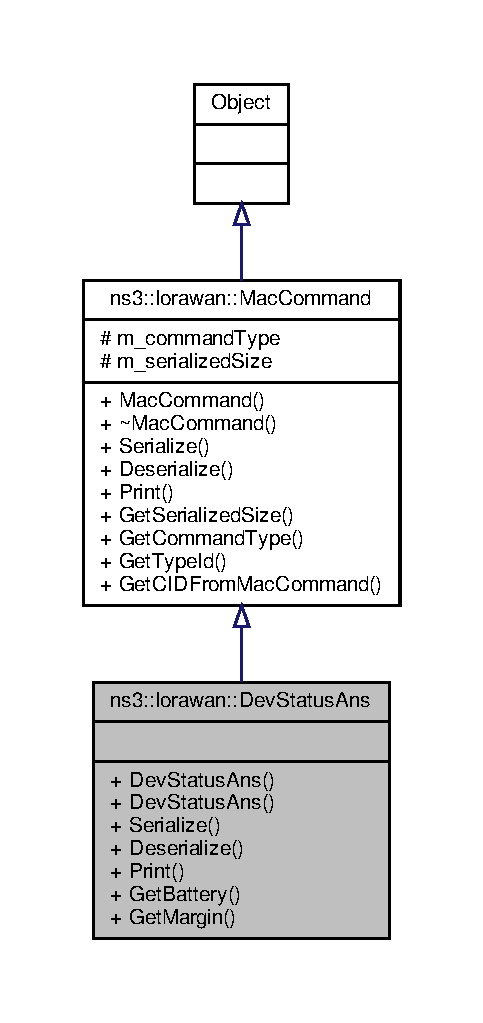
\includegraphics[width=232pt]{classns3_1_1lorawan_1_1DevStatusAns__inherit__graph}
\end{center}
\end{figure}


Collaboration diagram for ns3\+:\+:lorawan\+:\+:Dev\+Status\+Ans\+:
\nopagebreak
\begin{figure}[H]
\begin{center}
\leavevmode
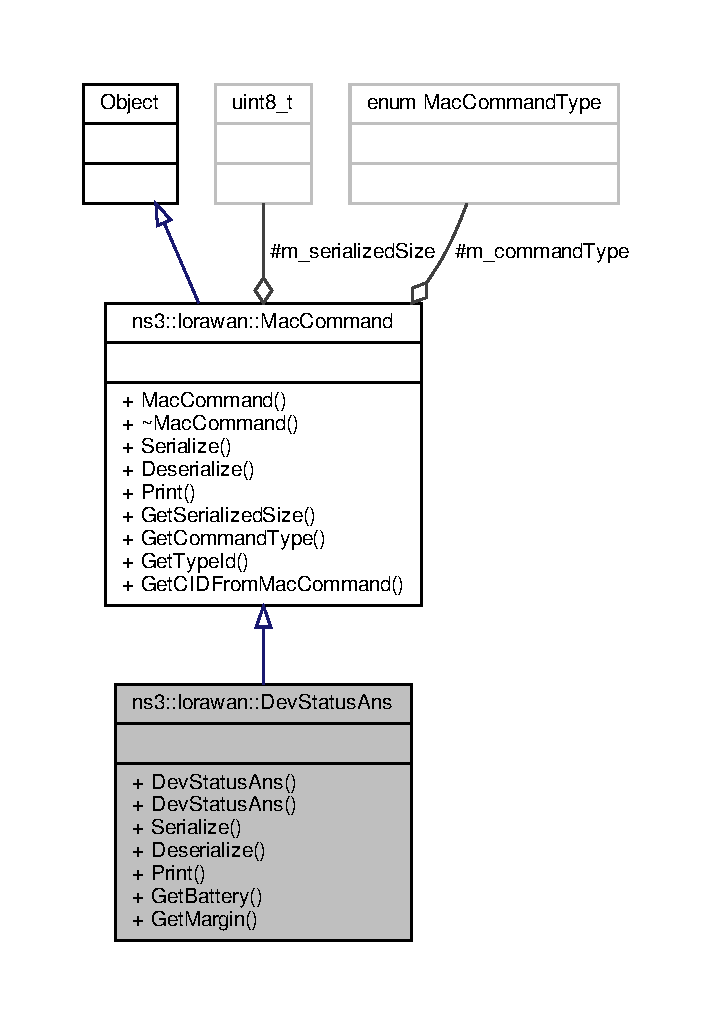
\includegraphics[width=343pt]{classns3_1_1lorawan_1_1DevStatusAns__coll__graph}
\end{center}
\end{figure}
\subsection*{Public Member Functions}
\begin{DoxyCompactItemize}
\item 
\hyperlink{classns3_1_1lorawan_1_1DevStatusAns_a2a117f790856a52f98743c42aaab5097}{Dev\+Status\+Ans} (uint8\+\_\+t battery, uint8\+\_\+t margin)
\item 
virtual void \hyperlink{classns3_1_1lorawan_1_1DevStatusAns_ab1e376c78c06b679eeb6d73d32aaa62f}{Serialize} (Buffer\+::\+Iterator \&start) const
\item 
virtual uint8\+\_\+t \hyperlink{classns3_1_1lorawan_1_1DevStatusAns_a359096eee9c97dd58abd5b37f2bcd059}{Deserialize} (Buffer\+::\+Iterator \&start)
\item 
virtual void \hyperlink{classns3_1_1lorawan_1_1DevStatusAns_a167cca1cb129a2084dcc5412a00b3126}{Print} (std\+::ostream \&os) const
\item 
uint8\+\_\+t \hyperlink{classns3_1_1lorawan_1_1DevStatusAns_a20703d8a96ccafe156ef0403912ac1c9}{Get\+Battery} (void)
\item 
uint8\+\_\+t \hyperlink{classns3_1_1lorawan_1_1DevStatusAns_a571f9538c6252bc91fe8dc7e7c6d0f11}{Get\+Margin} (void)
\end{DoxyCompactItemize}
\subsection*{Additional Inherited Members}


\subsection{Detailed Description}
Implementation of the \hyperlink{classns3_1_1lorawan_1_1DevStatusAns}{Dev\+Status\+Ans} Lo\+Ra\+W\+AN M\+AC command. 

\subsection{Constructor \& Destructor Documentation}
\mbox{\Hypertarget{classns3_1_1lorawan_1_1DevStatusAns_a2a117f790856a52f98743c42aaab5097}\label{classns3_1_1lorawan_1_1DevStatusAns_a2a117f790856a52f98743c42aaab5097}} 
\index{ns3\+::lorawan\+::\+Dev\+Status\+Ans@{ns3\+::lorawan\+::\+Dev\+Status\+Ans}!Dev\+Status\+Ans@{Dev\+Status\+Ans}}
\index{Dev\+Status\+Ans@{Dev\+Status\+Ans}!ns3\+::lorawan\+::\+Dev\+Status\+Ans@{ns3\+::lorawan\+::\+Dev\+Status\+Ans}}
\subsubsection{\texorpdfstring{Dev\+Status\+Ans()}{DevStatusAns()}}
{\footnotesize\ttfamily ns3\+::lorawan\+::\+Dev\+Status\+Ans\+::\+Dev\+Status\+Ans (\begin{DoxyParamCaption}\item[{uint8\+\_\+t}]{battery,  }\item[{uint8\+\_\+t}]{margin }\end{DoxyParamCaption})}

Constructor with initialization of all parameters.


\begin{DoxyParams}{Parameters}
{\em battery} & The battery level in \mbox{[}0, 255\mbox{]}. \\
\hline
{\em margin} & The demodulation margin of the last received \hyperlink{classns3_1_1lorawan_1_1DevStatusReq}{Dev\+Status\+Req} packet. \\
\hline
\end{DoxyParams}


\subsection{Member Function Documentation}
\mbox{\Hypertarget{classns3_1_1lorawan_1_1DevStatusAns_a359096eee9c97dd58abd5b37f2bcd059}\label{classns3_1_1lorawan_1_1DevStatusAns_a359096eee9c97dd58abd5b37f2bcd059}} 
\index{ns3\+::lorawan\+::\+Dev\+Status\+Ans@{ns3\+::lorawan\+::\+Dev\+Status\+Ans}!Deserialize@{Deserialize}}
\index{Deserialize@{Deserialize}!ns3\+::lorawan\+::\+Dev\+Status\+Ans@{ns3\+::lorawan\+::\+Dev\+Status\+Ans}}
\subsubsection{\texorpdfstring{Deserialize()}{Deserialize()}}
{\footnotesize\ttfamily uint8\+\_\+t ns3\+::lorawan\+::\+Dev\+Status\+Ans\+::\+Deserialize (\begin{DoxyParamCaption}\item[{Buffer\+::\+Iterator \&}]{start }\end{DoxyParamCaption})\hspace{0.3cm}{\ttfamily [virtual]}}

Deserialize the buffer into a M\+AC command.


\begin{DoxyParams}{Parameters}
{\em start} & A pointer to the buffer that contains the serialized command. \\
\hline
\end{DoxyParams}
\begin{DoxyReturn}{Returns}
the number of bytes that were consumed. 
\end{DoxyReturn}


Implements \hyperlink{classns3_1_1lorawan_1_1MacCommand_af12d223a71a67196bce498f1240eda75}{ns3\+::lorawan\+::\+Mac\+Command}.

\mbox{\Hypertarget{classns3_1_1lorawan_1_1DevStatusAns_a20703d8a96ccafe156ef0403912ac1c9}\label{classns3_1_1lorawan_1_1DevStatusAns_a20703d8a96ccafe156ef0403912ac1c9}} 
\index{ns3\+::lorawan\+::\+Dev\+Status\+Ans@{ns3\+::lorawan\+::\+Dev\+Status\+Ans}!Get\+Battery@{Get\+Battery}}
\index{Get\+Battery@{Get\+Battery}!ns3\+::lorawan\+::\+Dev\+Status\+Ans@{ns3\+::lorawan\+::\+Dev\+Status\+Ans}}
\subsubsection{\texorpdfstring{Get\+Battery()}{GetBattery()}}
{\footnotesize\ttfamily uint8\+\_\+t ns3\+::lorawan\+::\+Dev\+Status\+Ans\+::\+Get\+Battery (\begin{DoxyParamCaption}\item[{void}]{ }\end{DoxyParamCaption})}

Get the battery information contained in this M\+AC command.

\begin{DoxyReturn}{Returns}
The battery level. 
\end{DoxyReturn}
\mbox{\Hypertarget{classns3_1_1lorawan_1_1DevStatusAns_a571f9538c6252bc91fe8dc7e7c6d0f11}\label{classns3_1_1lorawan_1_1DevStatusAns_a571f9538c6252bc91fe8dc7e7c6d0f11}} 
\index{ns3\+::lorawan\+::\+Dev\+Status\+Ans@{ns3\+::lorawan\+::\+Dev\+Status\+Ans}!Get\+Margin@{Get\+Margin}}
\index{Get\+Margin@{Get\+Margin}!ns3\+::lorawan\+::\+Dev\+Status\+Ans@{ns3\+::lorawan\+::\+Dev\+Status\+Ans}}
\subsubsection{\texorpdfstring{Get\+Margin()}{GetMargin()}}
{\footnotesize\ttfamily uint8\+\_\+t ns3\+::lorawan\+::\+Dev\+Status\+Ans\+::\+Get\+Margin (\begin{DoxyParamCaption}\item[{void}]{ }\end{DoxyParamCaption})}

Get the demodulation margin contained in this M\+AC command.

\begin{DoxyReturn}{Returns}
The margin. 
\end{DoxyReturn}
\mbox{\Hypertarget{classns3_1_1lorawan_1_1DevStatusAns_a167cca1cb129a2084dcc5412a00b3126}\label{classns3_1_1lorawan_1_1DevStatusAns_a167cca1cb129a2084dcc5412a00b3126}} 
\index{ns3\+::lorawan\+::\+Dev\+Status\+Ans@{ns3\+::lorawan\+::\+Dev\+Status\+Ans}!Print@{Print}}
\index{Print@{Print}!ns3\+::lorawan\+::\+Dev\+Status\+Ans@{ns3\+::lorawan\+::\+Dev\+Status\+Ans}}
\subsubsection{\texorpdfstring{Print()}{Print()}}
{\footnotesize\ttfamily void ns3\+::lorawan\+::\+Dev\+Status\+Ans\+::\+Print (\begin{DoxyParamCaption}\item[{std\+::ostream \&}]{os }\end{DoxyParamCaption}) const\hspace{0.3cm}{\ttfamily [virtual]}}

Print the contents of this M\+AC command in human-\/readable format.


\begin{DoxyParams}{Parameters}
{\em os} & The std\+::ostream instance on which to print the M\+AC command. \\
\hline
\end{DoxyParams}


Implements \hyperlink{classns3_1_1lorawan_1_1MacCommand_a6bf88db38dab7dcd817811a9fb59f920}{ns3\+::lorawan\+::\+Mac\+Command}.

\mbox{\Hypertarget{classns3_1_1lorawan_1_1DevStatusAns_ab1e376c78c06b679eeb6d73d32aaa62f}\label{classns3_1_1lorawan_1_1DevStatusAns_ab1e376c78c06b679eeb6d73d32aaa62f}} 
\index{ns3\+::lorawan\+::\+Dev\+Status\+Ans@{ns3\+::lorawan\+::\+Dev\+Status\+Ans}!Serialize@{Serialize}}
\index{Serialize@{Serialize}!ns3\+::lorawan\+::\+Dev\+Status\+Ans@{ns3\+::lorawan\+::\+Dev\+Status\+Ans}}
\subsubsection{\texorpdfstring{Serialize()}{Serialize()}}
{\footnotesize\ttfamily void ns3\+::lorawan\+::\+Dev\+Status\+Ans\+::\+Serialize (\begin{DoxyParamCaption}\item[{Buffer\+::\+Iterator \&}]{start }\end{DoxyParamCaption}) const\hspace{0.3cm}{\ttfamily [virtual]}}

Serialize the contents of this M\+AC command into a buffer, according to the Lo\+Ra\+W\+AN standard.


\begin{DoxyParams}{Parameters}
{\em start} & A pointer to the buffer into which to serialize the command. \\
\hline
\end{DoxyParams}


Implements \hyperlink{classns3_1_1lorawan_1_1MacCommand_a0ed44b33942ddc3dc9694dc06ab0b87f}{ns3\+::lorawan\+::\+Mac\+Command}.



The documentation for this class was generated from the following files\+:\begin{DoxyCompactItemize}
\item 
mac-\/command.\+h\item 
mac-\/command.\+cc\end{DoxyCompactItemize}

\hypertarget{classns3_1_1lorawan_1_1DevStatusReq}{}\section{ns3\+:\+:lorawan\+:\+:Dev\+Status\+Req Class Reference}
\label{classns3_1_1lorawan_1_1DevStatusReq}\index{ns3\+::lorawan\+::\+Dev\+Status\+Req@{ns3\+::lorawan\+::\+Dev\+Status\+Req}}


{\ttfamily \#include $<$mac-\/command.\+h$>$}



Inheritance diagram for ns3\+:\+:lorawan\+:\+:Dev\+Status\+Req\+:
\nopagebreak
\begin{figure}[H]
\begin{center}
\leavevmode
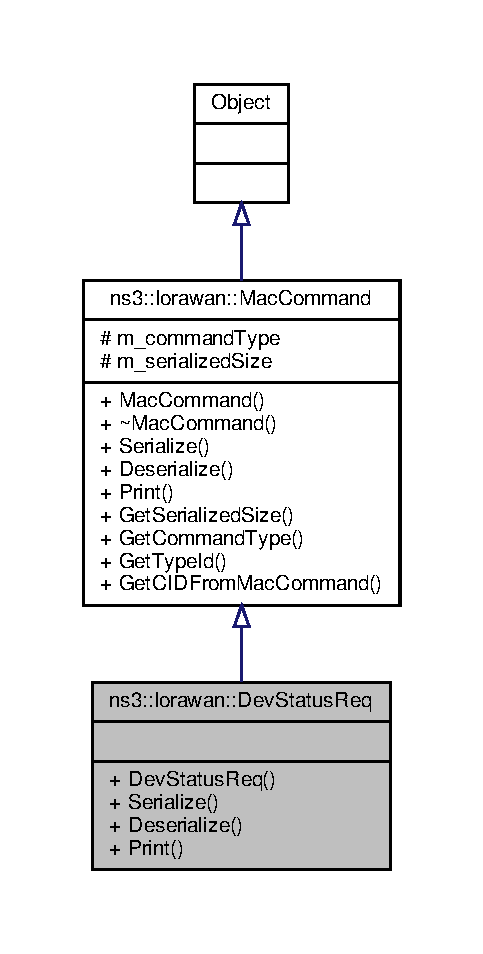
\includegraphics[width=232pt]{classns3_1_1lorawan_1_1DevStatusReq__inherit__graph}
\end{center}
\end{figure}


Collaboration diagram for ns3\+:\+:lorawan\+:\+:Dev\+Status\+Req\+:
\nopagebreak
\begin{figure}[H]
\begin{center}
\leavevmode
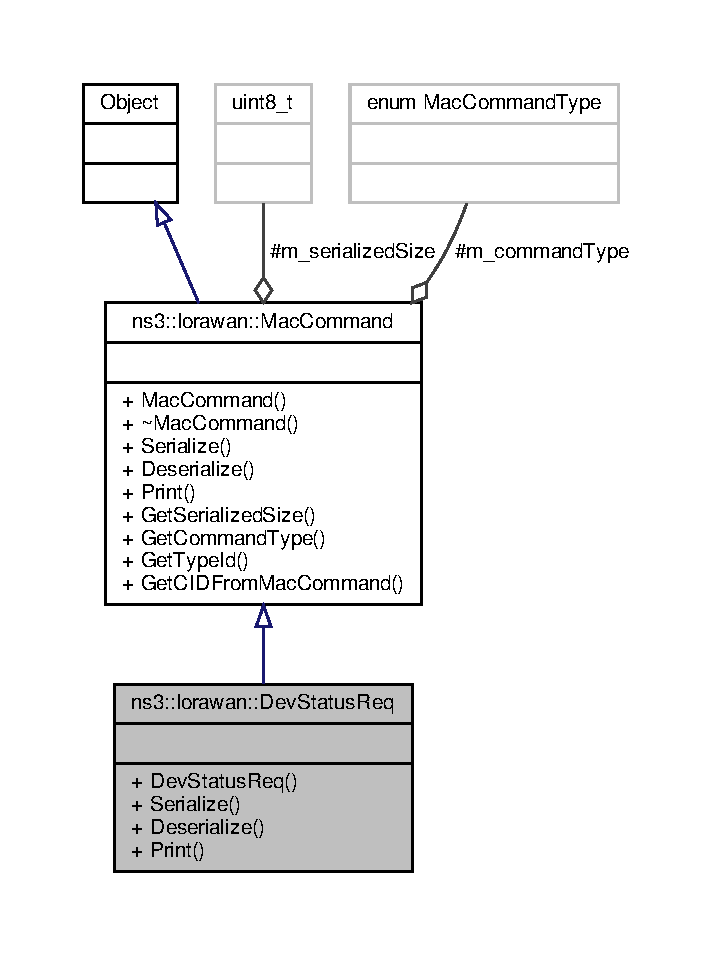
\includegraphics[width=343pt]{classns3_1_1lorawan_1_1DevStatusReq__coll__graph}
\end{center}
\end{figure}
\subsection*{Public Member Functions}
\begin{DoxyCompactItemize}
\item 
virtual void \hyperlink{classns3_1_1lorawan_1_1DevStatusReq_a98693e79ac85f1bf19980cc189ba27f6}{Serialize} (Buffer\+::\+Iterator \&start) const
\item 
virtual uint8\+\_\+t \hyperlink{classns3_1_1lorawan_1_1DevStatusReq_a6802f5824758e56ebe7317ba4a6d50b6}{Deserialize} (Buffer\+::\+Iterator \&start)
\item 
virtual void \hyperlink{classns3_1_1lorawan_1_1DevStatusReq_ad550f7d8f599f48d54dea36d87ab4ab9}{Print} (std\+::ostream \&os) const
\end{DoxyCompactItemize}
\subsection*{Additional Inherited Members}


\subsection{Detailed Description}
Implementation of the \hyperlink{classns3_1_1lorawan_1_1DevStatusReq}{Dev\+Status\+Req} Lo\+Ra\+W\+AN M\+AC command. 

\subsection{Member Function Documentation}
\mbox{\Hypertarget{classns3_1_1lorawan_1_1DevStatusReq_a6802f5824758e56ebe7317ba4a6d50b6}\label{classns3_1_1lorawan_1_1DevStatusReq_a6802f5824758e56ebe7317ba4a6d50b6}} 
\index{ns3\+::lorawan\+::\+Dev\+Status\+Req@{ns3\+::lorawan\+::\+Dev\+Status\+Req}!Deserialize@{Deserialize}}
\index{Deserialize@{Deserialize}!ns3\+::lorawan\+::\+Dev\+Status\+Req@{ns3\+::lorawan\+::\+Dev\+Status\+Req}}
\subsubsection{\texorpdfstring{Deserialize()}{Deserialize()}}
{\footnotesize\ttfamily uint8\+\_\+t ns3\+::lorawan\+::\+Dev\+Status\+Req\+::\+Deserialize (\begin{DoxyParamCaption}\item[{Buffer\+::\+Iterator \&}]{start }\end{DoxyParamCaption})\hspace{0.3cm}{\ttfamily [virtual]}}

Deserialize the buffer into a M\+AC command.


\begin{DoxyParams}{Parameters}
{\em start} & A pointer to the buffer that contains the serialized command. \\
\hline
\end{DoxyParams}
\begin{DoxyReturn}{Returns}
the number of bytes that were consumed. 
\end{DoxyReturn}


Implements \hyperlink{classns3_1_1lorawan_1_1MacCommand_af12d223a71a67196bce498f1240eda75}{ns3\+::lorawan\+::\+Mac\+Command}.

\mbox{\Hypertarget{classns3_1_1lorawan_1_1DevStatusReq_ad550f7d8f599f48d54dea36d87ab4ab9}\label{classns3_1_1lorawan_1_1DevStatusReq_ad550f7d8f599f48d54dea36d87ab4ab9}} 
\index{ns3\+::lorawan\+::\+Dev\+Status\+Req@{ns3\+::lorawan\+::\+Dev\+Status\+Req}!Print@{Print}}
\index{Print@{Print}!ns3\+::lorawan\+::\+Dev\+Status\+Req@{ns3\+::lorawan\+::\+Dev\+Status\+Req}}
\subsubsection{\texorpdfstring{Print()}{Print()}}
{\footnotesize\ttfamily void ns3\+::lorawan\+::\+Dev\+Status\+Req\+::\+Print (\begin{DoxyParamCaption}\item[{std\+::ostream \&}]{os }\end{DoxyParamCaption}) const\hspace{0.3cm}{\ttfamily [virtual]}}

Print the contents of this M\+AC command in human-\/readable format.


\begin{DoxyParams}{Parameters}
{\em os} & The std\+::ostream instance on which to print the M\+AC command. \\
\hline
\end{DoxyParams}


Implements \hyperlink{classns3_1_1lorawan_1_1MacCommand_a6bf88db38dab7dcd817811a9fb59f920}{ns3\+::lorawan\+::\+Mac\+Command}.

\mbox{\Hypertarget{classns3_1_1lorawan_1_1DevStatusReq_a98693e79ac85f1bf19980cc189ba27f6}\label{classns3_1_1lorawan_1_1DevStatusReq_a98693e79ac85f1bf19980cc189ba27f6}} 
\index{ns3\+::lorawan\+::\+Dev\+Status\+Req@{ns3\+::lorawan\+::\+Dev\+Status\+Req}!Serialize@{Serialize}}
\index{Serialize@{Serialize}!ns3\+::lorawan\+::\+Dev\+Status\+Req@{ns3\+::lorawan\+::\+Dev\+Status\+Req}}
\subsubsection{\texorpdfstring{Serialize()}{Serialize()}}
{\footnotesize\ttfamily void ns3\+::lorawan\+::\+Dev\+Status\+Req\+::\+Serialize (\begin{DoxyParamCaption}\item[{Buffer\+::\+Iterator \&}]{start }\end{DoxyParamCaption}) const\hspace{0.3cm}{\ttfamily [virtual]}}

Serialize the contents of this M\+AC command into a buffer, according to the Lo\+Ra\+W\+AN standard.


\begin{DoxyParams}{Parameters}
{\em start} & A pointer to the buffer into which to serialize the command. \\
\hline
\end{DoxyParams}


Implements \hyperlink{classns3_1_1lorawan_1_1MacCommand_a0ed44b33942ddc3dc9694dc06ab0b87f}{ns3\+::lorawan\+::\+Mac\+Command}.



The documentation for this class was generated from the following files\+:\begin{DoxyCompactItemize}
\item 
mac-\/command.\+h\item 
mac-\/command.\+cc\end{DoxyCompactItemize}

\hypertarget{classns3_1_1lorawan_1_1DlChannelAns}{}\section{ns3\+:\+:lorawan\+:\+:Dl\+Channel\+Ans Class Reference}
\label{classns3_1_1lorawan_1_1DlChannelAns}\index{ns3\+::lorawan\+::\+Dl\+Channel\+Ans@{ns3\+::lorawan\+::\+Dl\+Channel\+Ans}}


{\ttfamily \#include $<$mac-\/command.\+h$>$}



Inheritance diagram for ns3\+:\+:lorawan\+:\+:Dl\+Channel\+Ans\+:
\nopagebreak
\begin{figure}[H]
\begin{center}
\leavevmode
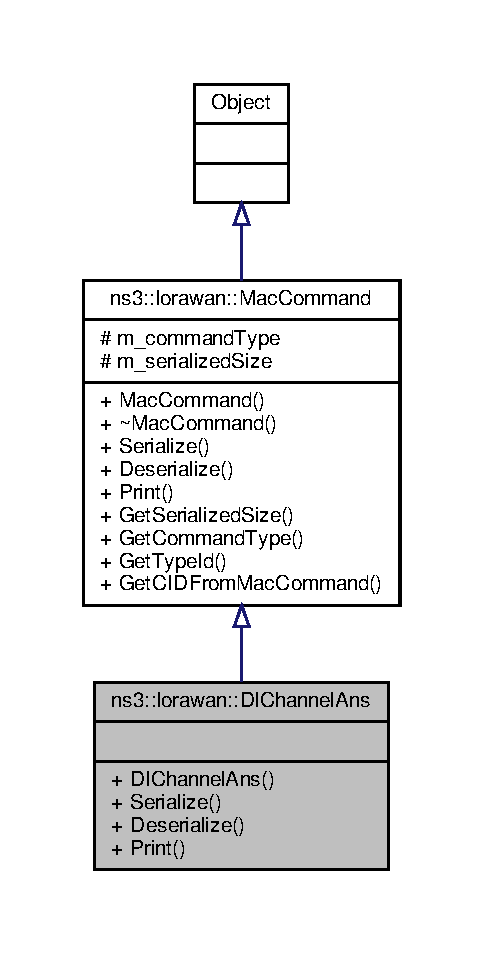
\includegraphics[width=232pt]{classns3_1_1lorawan_1_1DlChannelAns__inherit__graph}
\end{center}
\end{figure}


Collaboration diagram for ns3\+:\+:lorawan\+:\+:Dl\+Channel\+Ans\+:
\nopagebreak
\begin{figure}[H]
\begin{center}
\leavevmode
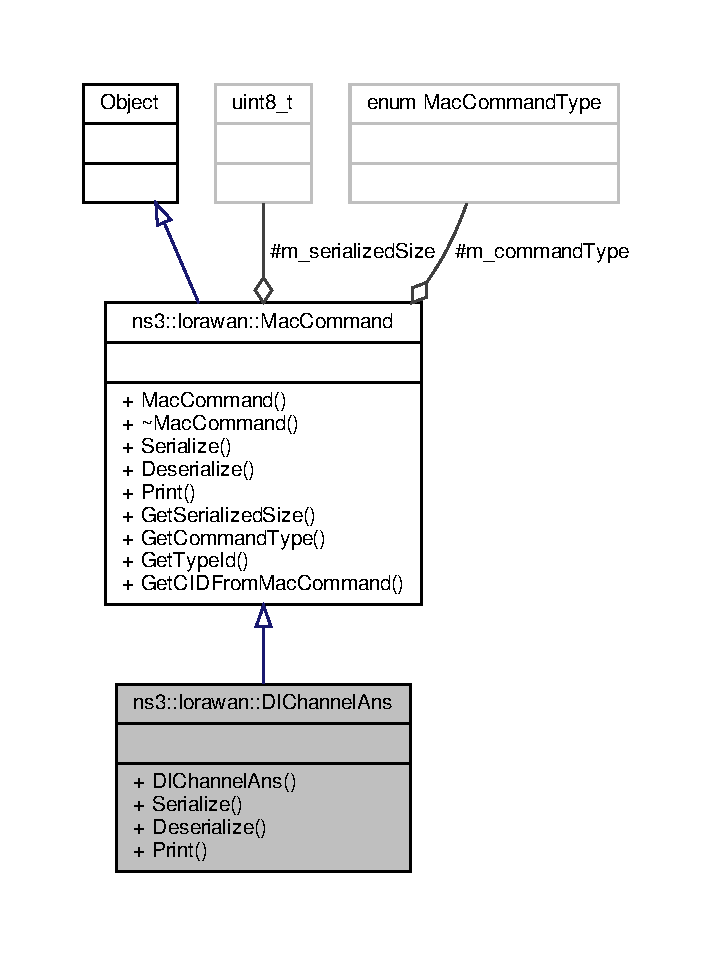
\includegraphics[width=343pt]{classns3_1_1lorawan_1_1DlChannelAns__coll__graph}
\end{center}
\end{figure}
\subsection*{Public Member Functions}
\begin{DoxyCompactItemize}
\item 
virtual void \hyperlink{classns3_1_1lorawan_1_1DlChannelAns_a9fef6b765888e26a0031757b435028a0}{Serialize} (Buffer\+::\+Iterator \&start) const
\item 
virtual uint8\+\_\+t \hyperlink{classns3_1_1lorawan_1_1DlChannelAns_a15482fde8754d5fa211754ef2352e514}{Deserialize} (Buffer\+::\+Iterator \&start)
\item 
virtual void \hyperlink{classns3_1_1lorawan_1_1DlChannelAns_a1dbe96549927ce3aa98c8d68a341f5bd}{Print} (std\+::ostream \&os) const
\end{DoxyCompactItemize}
\subsection*{Additional Inherited Members}


\subsection{Detailed Description}
Implementation of the \hyperlink{classns3_1_1lorawan_1_1DlChannelAns}{Dl\+Channel\+Ans} Lo\+Ra\+W\+AN M\+AC command. 

\subsection{Member Function Documentation}
\mbox{\Hypertarget{classns3_1_1lorawan_1_1DlChannelAns_a15482fde8754d5fa211754ef2352e514}\label{classns3_1_1lorawan_1_1DlChannelAns_a15482fde8754d5fa211754ef2352e514}} 
\index{ns3\+::lorawan\+::\+Dl\+Channel\+Ans@{ns3\+::lorawan\+::\+Dl\+Channel\+Ans}!Deserialize@{Deserialize}}
\index{Deserialize@{Deserialize}!ns3\+::lorawan\+::\+Dl\+Channel\+Ans@{ns3\+::lorawan\+::\+Dl\+Channel\+Ans}}
\subsubsection{\texorpdfstring{Deserialize()}{Deserialize()}}
{\footnotesize\ttfamily uint8\+\_\+t ns3\+::lorawan\+::\+Dl\+Channel\+Ans\+::\+Deserialize (\begin{DoxyParamCaption}\item[{Buffer\+::\+Iterator \&}]{start }\end{DoxyParamCaption})\hspace{0.3cm}{\ttfamily [virtual]}}

Deserialize the buffer into a M\+AC command.


\begin{DoxyParams}{Parameters}
{\em start} & A pointer to the buffer that contains the serialized command. \\
\hline
\end{DoxyParams}
\begin{DoxyReturn}{Returns}
the number of bytes that were consumed. 
\end{DoxyReturn}


Implements \hyperlink{classns3_1_1lorawan_1_1MacCommand_af12d223a71a67196bce498f1240eda75}{ns3\+::lorawan\+::\+Mac\+Command}.

\mbox{\Hypertarget{classns3_1_1lorawan_1_1DlChannelAns_a1dbe96549927ce3aa98c8d68a341f5bd}\label{classns3_1_1lorawan_1_1DlChannelAns_a1dbe96549927ce3aa98c8d68a341f5bd}} 
\index{ns3\+::lorawan\+::\+Dl\+Channel\+Ans@{ns3\+::lorawan\+::\+Dl\+Channel\+Ans}!Print@{Print}}
\index{Print@{Print}!ns3\+::lorawan\+::\+Dl\+Channel\+Ans@{ns3\+::lorawan\+::\+Dl\+Channel\+Ans}}
\subsubsection{\texorpdfstring{Print()}{Print()}}
{\footnotesize\ttfamily void ns3\+::lorawan\+::\+Dl\+Channel\+Ans\+::\+Print (\begin{DoxyParamCaption}\item[{std\+::ostream \&}]{os }\end{DoxyParamCaption}) const\hspace{0.3cm}{\ttfamily [virtual]}}

Print the contents of this M\+AC command in human-\/readable format.


\begin{DoxyParams}{Parameters}
{\em os} & The std\+::ostream instance on which to print the M\+AC command. \\
\hline
\end{DoxyParams}


Implements \hyperlink{classns3_1_1lorawan_1_1MacCommand_a6bf88db38dab7dcd817811a9fb59f920}{ns3\+::lorawan\+::\+Mac\+Command}.

\mbox{\Hypertarget{classns3_1_1lorawan_1_1DlChannelAns_a9fef6b765888e26a0031757b435028a0}\label{classns3_1_1lorawan_1_1DlChannelAns_a9fef6b765888e26a0031757b435028a0}} 
\index{ns3\+::lorawan\+::\+Dl\+Channel\+Ans@{ns3\+::lorawan\+::\+Dl\+Channel\+Ans}!Serialize@{Serialize}}
\index{Serialize@{Serialize}!ns3\+::lorawan\+::\+Dl\+Channel\+Ans@{ns3\+::lorawan\+::\+Dl\+Channel\+Ans}}
\subsubsection{\texorpdfstring{Serialize()}{Serialize()}}
{\footnotesize\ttfamily void ns3\+::lorawan\+::\+Dl\+Channel\+Ans\+::\+Serialize (\begin{DoxyParamCaption}\item[{Buffer\+::\+Iterator \&}]{start }\end{DoxyParamCaption}) const\hspace{0.3cm}{\ttfamily [virtual]}}

Serialize the contents of this M\+AC command into a buffer, according to the Lo\+Ra\+W\+AN standard.


\begin{DoxyParams}{Parameters}
{\em start} & A pointer to the buffer into which to serialize the command. \\
\hline
\end{DoxyParams}


Implements \hyperlink{classns3_1_1lorawan_1_1MacCommand_a0ed44b33942ddc3dc9694dc06ab0b87f}{ns3\+::lorawan\+::\+Mac\+Command}.



The documentation for this class was generated from the following files\+:\begin{DoxyCompactItemize}
\item 
mac-\/command.\+h\item 
mac-\/command.\+cc\end{DoxyCompactItemize}

\hypertarget{classns3_1_1lorawan_1_1DutyCycleAns}{}\section{ns3\+:\+:lorawan\+:\+:Duty\+Cycle\+Ans Class Reference}
\label{classns3_1_1lorawan_1_1DutyCycleAns}\index{ns3\+::lorawan\+::\+Duty\+Cycle\+Ans@{ns3\+::lorawan\+::\+Duty\+Cycle\+Ans}}


{\ttfamily \#include $<$mac-\/command.\+h$>$}



Inheritance diagram for ns3\+:\+:lorawan\+:\+:Duty\+Cycle\+Ans\+:
\nopagebreak
\begin{figure}[H]
\begin{center}
\leavevmode
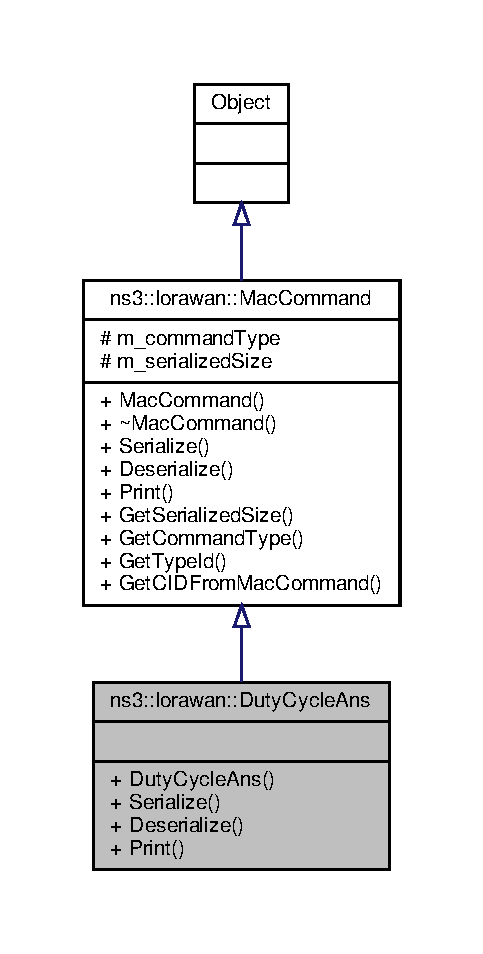
\includegraphics[width=232pt]{classns3_1_1lorawan_1_1DutyCycleAns__inherit__graph}
\end{center}
\end{figure}


Collaboration diagram for ns3\+:\+:lorawan\+:\+:Duty\+Cycle\+Ans\+:
\nopagebreak
\begin{figure}[H]
\begin{center}
\leavevmode
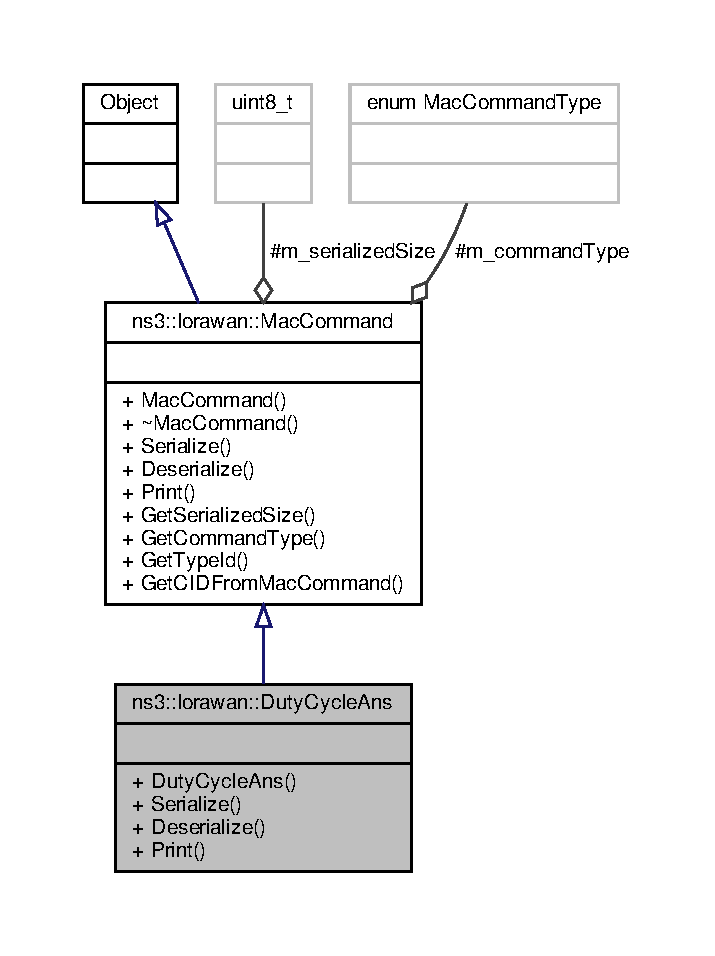
\includegraphics[width=343pt]{classns3_1_1lorawan_1_1DutyCycleAns__coll__graph}
\end{center}
\end{figure}
\subsection*{Public Member Functions}
\begin{DoxyCompactItemize}
\item 
virtual void \hyperlink{classns3_1_1lorawan_1_1DutyCycleAns_aff6f7b100eba491c770be23c342e5f87}{Serialize} (Buffer\+::\+Iterator \&start) const
\item 
virtual uint8\+\_\+t \hyperlink{classns3_1_1lorawan_1_1DutyCycleAns_aa3157f0326048cb774c8cfeb0f6d35a7}{Deserialize} (Buffer\+::\+Iterator \&start)
\item 
virtual void \hyperlink{classns3_1_1lorawan_1_1DutyCycleAns_a201b7cdda81f6b775f13da09ba675e26}{Print} (std\+::ostream \&os) const
\end{DoxyCompactItemize}
\subsection*{Additional Inherited Members}


\subsection{Detailed Description}
Implementation of the \hyperlink{classns3_1_1lorawan_1_1DutyCycleAns}{Duty\+Cycle\+Ans} Lo\+Ra\+W\+AN M\+AC command.

This command holds no variables, and just consists in the C\+ID. 

\subsection{Member Function Documentation}
\mbox{\Hypertarget{classns3_1_1lorawan_1_1DutyCycleAns_aa3157f0326048cb774c8cfeb0f6d35a7}\label{classns3_1_1lorawan_1_1DutyCycleAns_aa3157f0326048cb774c8cfeb0f6d35a7}} 
\index{ns3\+::lorawan\+::\+Duty\+Cycle\+Ans@{ns3\+::lorawan\+::\+Duty\+Cycle\+Ans}!Deserialize@{Deserialize}}
\index{Deserialize@{Deserialize}!ns3\+::lorawan\+::\+Duty\+Cycle\+Ans@{ns3\+::lorawan\+::\+Duty\+Cycle\+Ans}}
\subsubsection{\texorpdfstring{Deserialize()}{Deserialize()}}
{\footnotesize\ttfamily uint8\+\_\+t ns3\+::lorawan\+::\+Duty\+Cycle\+Ans\+::\+Deserialize (\begin{DoxyParamCaption}\item[{Buffer\+::\+Iterator \&}]{start }\end{DoxyParamCaption})\hspace{0.3cm}{\ttfamily [virtual]}}

Deserialize the buffer into a M\+AC command.


\begin{DoxyParams}{Parameters}
{\em start} & A pointer to the buffer that contains the serialized command. \\
\hline
\end{DoxyParams}
\begin{DoxyReturn}{Returns}
the number of bytes that were consumed. 
\end{DoxyReturn}


Implements \hyperlink{classns3_1_1lorawan_1_1MacCommand_af12d223a71a67196bce498f1240eda75}{ns3\+::lorawan\+::\+Mac\+Command}.

\mbox{\Hypertarget{classns3_1_1lorawan_1_1DutyCycleAns_a201b7cdda81f6b775f13da09ba675e26}\label{classns3_1_1lorawan_1_1DutyCycleAns_a201b7cdda81f6b775f13da09ba675e26}} 
\index{ns3\+::lorawan\+::\+Duty\+Cycle\+Ans@{ns3\+::lorawan\+::\+Duty\+Cycle\+Ans}!Print@{Print}}
\index{Print@{Print}!ns3\+::lorawan\+::\+Duty\+Cycle\+Ans@{ns3\+::lorawan\+::\+Duty\+Cycle\+Ans}}
\subsubsection{\texorpdfstring{Print()}{Print()}}
{\footnotesize\ttfamily void ns3\+::lorawan\+::\+Duty\+Cycle\+Ans\+::\+Print (\begin{DoxyParamCaption}\item[{std\+::ostream \&}]{os }\end{DoxyParamCaption}) const\hspace{0.3cm}{\ttfamily [virtual]}}

Print the contents of this M\+AC command in human-\/readable format.


\begin{DoxyParams}{Parameters}
{\em os} & The std\+::ostream instance on which to print the M\+AC command. \\
\hline
\end{DoxyParams}


Implements \hyperlink{classns3_1_1lorawan_1_1MacCommand_a6bf88db38dab7dcd817811a9fb59f920}{ns3\+::lorawan\+::\+Mac\+Command}.

\mbox{\Hypertarget{classns3_1_1lorawan_1_1DutyCycleAns_aff6f7b100eba491c770be23c342e5f87}\label{classns3_1_1lorawan_1_1DutyCycleAns_aff6f7b100eba491c770be23c342e5f87}} 
\index{ns3\+::lorawan\+::\+Duty\+Cycle\+Ans@{ns3\+::lorawan\+::\+Duty\+Cycle\+Ans}!Serialize@{Serialize}}
\index{Serialize@{Serialize}!ns3\+::lorawan\+::\+Duty\+Cycle\+Ans@{ns3\+::lorawan\+::\+Duty\+Cycle\+Ans}}
\subsubsection{\texorpdfstring{Serialize()}{Serialize()}}
{\footnotesize\ttfamily void ns3\+::lorawan\+::\+Duty\+Cycle\+Ans\+::\+Serialize (\begin{DoxyParamCaption}\item[{Buffer\+::\+Iterator \&}]{start }\end{DoxyParamCaption}) const\hspace{0.3cm}{\ttfamily [virtual]}}

Serialize the contents of this M\+AC command into a buffer, according to the Lo\+Ra\+W\+AN standard.


\begin{DoxyParams}{Parameters}
{\em start} & A pointer to the buffer into which to serialize the command. \\
\hline
\end{DoxyParams}


Implements \hyperlink{classns3_1_1lorawan_1_1MacCommand_a0ed44b33942ddc3dc9694dc06ab0b87f}{ns3\+::lorawan\+::\+Mac\+Command}.



The documentation for this class was generated from the following files\+:\begin{DoxyCompactItemize}
\item 
mac-\/command.\+h\item 
mac-\/command.\+cc\end{DoxyCompactItemize}

\hypertarget{classns3_1_1lorawan_1_1DutyCycleReq}{}\section{ns3\+:\+:lorawan\+:\+:Duty\+Cycle\+Req Class Reference}
\label{classns3_1_1lorawan_1_1DutyCycleReq}\index{ns3\+::lorawan\+::\+Duty\+Cycle\+Req@{ns3\+::lorawan\+::\+Duty\+Cycle\+Req}}


{\ttfamily \#include $<$mac-\/command.\+h$>$}



Inheritance diagram for ns3\+:\+:lorawan\+:\+:Duty\+Cycle\+Req\+:
\nopagebreak
\begin{figure}[H]
\begin{center}
\leavevmode
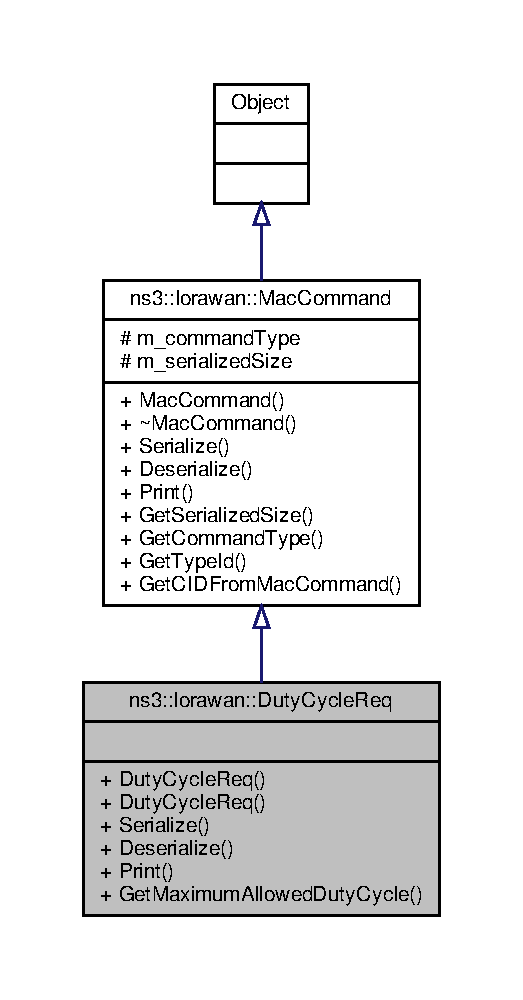
\includegraphics[width=251pt]{classns3_1_1lorawan_1_1DutyCycleReq__inherit__graph}
\end{center}
\end{figure}


Collaboration diagram for ns3\+:\+:lorawan\+:\+:Duty\+Cycle\+Req\+:
\nopagebreak
\begin{figure}[H]
\begin{center}
\leavevmode
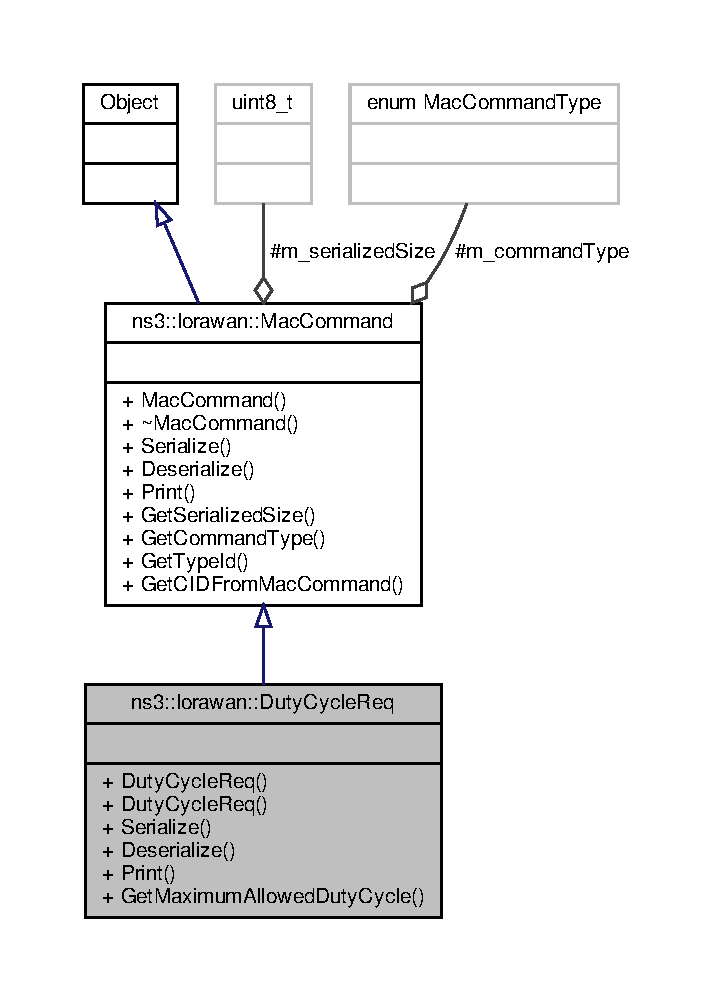
\includegraphics[width=343pt]{classns3_1_1lorawan_1_1DutyCycleReq__coll__graph}
\end{center}
\end{figure}
\subsection*{Public Member Functions}
\begin{DoxyCompactItemize}
\item 
\hyperlink{classns3_1_1lorawan_1_1DutyCycleReq_aa940e6c73680a6eadfa976d08b56f92c}{Duty\+Cycle\+Req} (uint8\+\_\+t duty\+Cycle)
\item 
virtual void \hyperlink{classns3_1_1lorawan_1_1DutyCycleReq_ae8bd08eaf66d3a83f4c972d6317bc7dd}{Serialize} (Buffer\+::\+Iterator \&start) const
\item 
virtual uint8\+\_\+t \hyperlink{classns3_1_1lorawan_1_1DutyCycleReq_ac158ec7e1539555825e2651ee176c7a5}{Deserialize} (Buffer\+::\+Iterator \&start)
\item 
virtual void \hyperlink{classns3_1_1lorawan_1_1DutyCycleReq_a8d0d86de5e54eab057bcdd9b79c97aa9}{Print} (std\+::ostream \&os) const
\item 
double \hyperlink{classns3_1_1lorawan_1_1DutyCycleReq_ab42bcc06f2f90bac5aaf3a267fed20e8}{Get\+Maximum\+Allowed\+Duty\+Cycle} (void) const
\end{DoxyCompactItemize}
\subsection*{Additional Inherited Members}


\subsection{Detailed Description}
Implementation of the \hyperlink{classns3_1_1lorawan_1_1DutyCycleReq}{Duty\+Cycle\+Req} Lo\+Ra\+W\+AN M\+AC command.

With this command, the network server can limit the maximum aggregated transmit duty cycle of an end device. The aggregate duty cycle is computed as the duty cycle among all sub bands. 

\subsection{Constructor \& Destructor Documentation}
\mbox{\Hypertarget{classns3_1_1lorawan_1_1DutyCycleReq_aa940e6c73680a6eadfa976d08b56f92c}\label{classns3_1_1lorawan_1_1DutyCycleReq_aa940e6c73680a6eadfa976d08b56f92c}} 
\index{ns3\+::lorawan\+::\+Duty\+Cycle\+Req@{ns3\+::lorawan\+::\+Duty\+Cycle\+Req}!Duty\+Cycle\+Req@{Duty\+Cycle\+Req}}
\index{Duty\+Cycle\+Req@{Duty\+Cycle\+Req}!ns3\+::lorawan\+::\+Duty\+Cycle\+Req@{ns3\+::lorawan\+::\+Duty\+Cycle\+Req}}
\subsubsection{\texorpdfstring{Duty\+Cycle\+Req()}{DutyCycleReq()}}
{\footnotesize\ttfamily ns3\+::lorawan\+::\+Duty\+Cycle\+Req\+::\+Duty\+Cycle\+Req (\begin{DoxyParamCaption}\item[{uint8\+\_\+t}]{duty\+Cycle }\end{DoxyParamCaption})}

Constructor providing initialization of all parameters.


\begin{DoxyParams}{Parameters}
{\em duty\+Cycle} & The duty cycle as a 8-\/bit unsigned integer. \\
\hline
\end{DoxyParams}


\subsection{Member Function Documentation}
\mbox{\Hypertarget{classns3_1_1lorawan_1_1DutyCycleReq_ac158ec7e1539555825e2651ee176c7a5}\label{classns3_1_1lorawan_1_1DutyCycleReq_ac158ec7e1539555825e2651ee176c7a5}} 
\index{ns3\+::lorawan\+::\+Duty\+Cycle\+Req@{ns3\+::lorawan\+::\+Duty\+Cycle\+Req}!Deserialize@{Deserialize}}
\index{Deserialize@{Deserialize}!ns3\+::lorawan\+::\+Duty\+Cycle\+Req@{ns3\+::lorawan\+::\+Duty\+Cycle\+Req}}
\subsubsection{\texorpdfstring{Deserialize()}{Deserialize()}}
{\footnotesize\ttfamily uint8\+\_\+t ns3\+::lorawan\+::\+Duty\+Cycle\+Req\+::\+Deserialize (\begin{DoxyParamCaption}\item[{Buffer\+::\+Iterator \&}]{start }\end{DoxyParamCaption})\hspace{0.3cm}{\ttfamily [virtual]}}

Deserialize the buffer into a M\+AC command.


\begin{DoxyParams}{Parameters}
{\em start} & A pointer to the buffer that contains the serialized command. \\
\hline
\end{DoxyParams}
\begin{DoxyReturn}{Returns}
the number of bytes that were consumed. 
\end{DoxyReturn}


Implements \hyperlink{classns3_1_1lorawan_1_1MacCommand_af12d223a71a67196bce498f1240eda75}{ns3\+::lorawan\+::\+Mac\+Command}.

\mbox{\Hypertarget{classns3_1_1lorawan_1_1DutyCycleReq_ab42bcc06f2f90bac5aaf3a267fed20e8}\label{classns3_1_1lorawan_1_1DutyCycleReq_ab42bcc06f2f90bac5aaf3a267fed20e8}} 
\index{ns3\+::lorawan\+::\+Duty\+Cycle\+Req@{ns3\+::lorawan\+::\+Duty\+Cycle\+Req}!Get\+Maximum\+Allowed\+Duty\+Cycle@{Get\+Maximum\+Allowed\+Duty\+Cycle}}
\index{Get\+Maximum\+Allowed\+Duty\+Cycle@{Get\+Maximum\+Allowed\+Duty\+Cycle}!ns3\+::lorawan\+::\+Duty\+Cycle\+Req@{ns3\+::lorawan\+::\+Duty\+Cycle\+Req}}
\subsubsection{\texorpdfstring{Get\+Maximum\+Allowed\+Duty\+Cycle()}{GetMaximumAllowedDutyCycle()}}
{\footnotesize\ttfamily double ns3\+::lorawan\+::\+Duty\+Cycle\+Req\+::\+Get\+Maximum\+Allowed\+Duty\+Cycle (\begin{DoxyParamCaption}\item[{void}]{ }\end{DoxyParamCaption}) const}

Get the maximum duty cycle prescribed by this Mac command, in fraction form.

\begin{DoxyReturn}{Returns}
The maximum duty cycle. 
\end{DoxyReturn}
\mbox{\Hypertarget{classns3_1_1lorawan_1_1DutyCycleReq_a8d0d86de5e54eab057bcdd9b79c97aa9}\label{classns3_1_1lorawan_1_1DutyCycleReq_a8d0d86de5e54eab057bcdd9b79c97aa9}} 
\index{ns3\+::lorawan\+::\+Duty\+Cycle\+Req@{ns3\+::lorawan\+::\+Duty\+Cycle\+Req}!Print@{Print}}
\index{Print@{Print}!ns3\+::lorawan\+::\+Duty\+Cycle\+Req@{ns3\+::lorawan\+::\+Duty\+Cycle\+Req}}
\subsubsection{\texorpdfstring{Print()}{Print()}}
{\footnotesize\ttfamily void ns3\+::lorawan\+::\+Duty\+Cycle\+Req\+::\+Print (\begin{DoxyParamCaption}\item[{std\+::ostream \&}]{os }\end{DoxyParamCaption}) const\hspace{0.3cm}{\ttfamily [virtual]}}

Print the contents of this M\+AC command in human-\/readable format.


\begin{DoxyParams}{Parameters}
{\em os} & The std\+::ostream instance on which to print the M\+AC command. \\
\hline
\end{DoxyParams}


Implements \hyperlink{classns3_1_1lorawan_1_1MacCommand_a6bf88db38dab7dcd817811a9fb59f920}{ns3\+::lorawan\+::\+Mac\+Command}.

\mbox{\Hypertarget{classns3_1_1lorawan_1_1DutyCycleReq_ae8bd08eaf66d3a83f4c972d6317bc7dd}\label{classns3_1_1lorawan_1_1DutyCycleReq_ae8bd08eaf66d3a83f4c972d6317bc7dd}} 
\index{ns3\+::lorawan\+::\+Duty\+Cycle\+Req@{ns3\+::lorawan\+::\+Duty\+Cycle\+Req}!Serialize@{Serialize}}
\index{Serialize@{Serialize}!ns3\+::lorawan\+::\+Duty\+Cycle\+Req@{ns3\+::lorawan\+::\+Duty\+Cycle\+Req}}
\subsubsection{\texorpdfstring{Serialize()}{Serialize()}}
{\footnotesize\ttfamily void ns3\+::lorawan\+::\+Duty\+Cycle\+Req\+::\+Serialize (\begin{DoxyParamCaption}\item[{Buffer\+::\+Iterator \&}]{start }\end{DoxyParamCaption}) const\hspace{0.3cm}{\ttfamily [virtual]}}

Serialize the contents of this M\+AC command into a buffer, according to the Lo\+Ra\+W\+AN standard.


\begin{DoxyParams}{Parameters}
{\em start} & A pointer to the buffer into which to serialize the command. \\
\hline
\end{DoxyParams}


Implements \hyperlink{classns3_1_1lorawan_1_1MacCommand_a0ed44b33942ddc3dc9694dc06ab0b87f}{ns3\+::lorawan\+::\+Mac\+Command}.



The documentation for this class was generated from the following files\+:\begin{DoxyCompactItemize}
\item 
mac-\/command.\+h\item 
mac-\/command.\+cc\end{DoxyCompactItemize}

\hypertarget{classns3_1_1lorawan_1_1EndDeviceLoraMac}{}\section{ns3\+:\+:lorawan\+:\+:End\+Device\+Lora\+Mac Class Reference}
\label{classns3_1_1lorawan_1_1EndDeviceLoraMac}\index{ns3\+::lorawan\+::\+End\+Device\+Lora\+Mac@{ns3\+::lorawan\+::\+End\+Device\+Lora\+Mac}}


{\ttfamily \#include $<$end-\/device-\/lora-\/mac.\+h$>$}



Inheritance diagram for ns3\+:\+:lorawan\+:\+:End\+Device\+Lora\+Mac\+:
\nopagebreak
\begin{figure}[H]
\begin{center}
\leavevmode
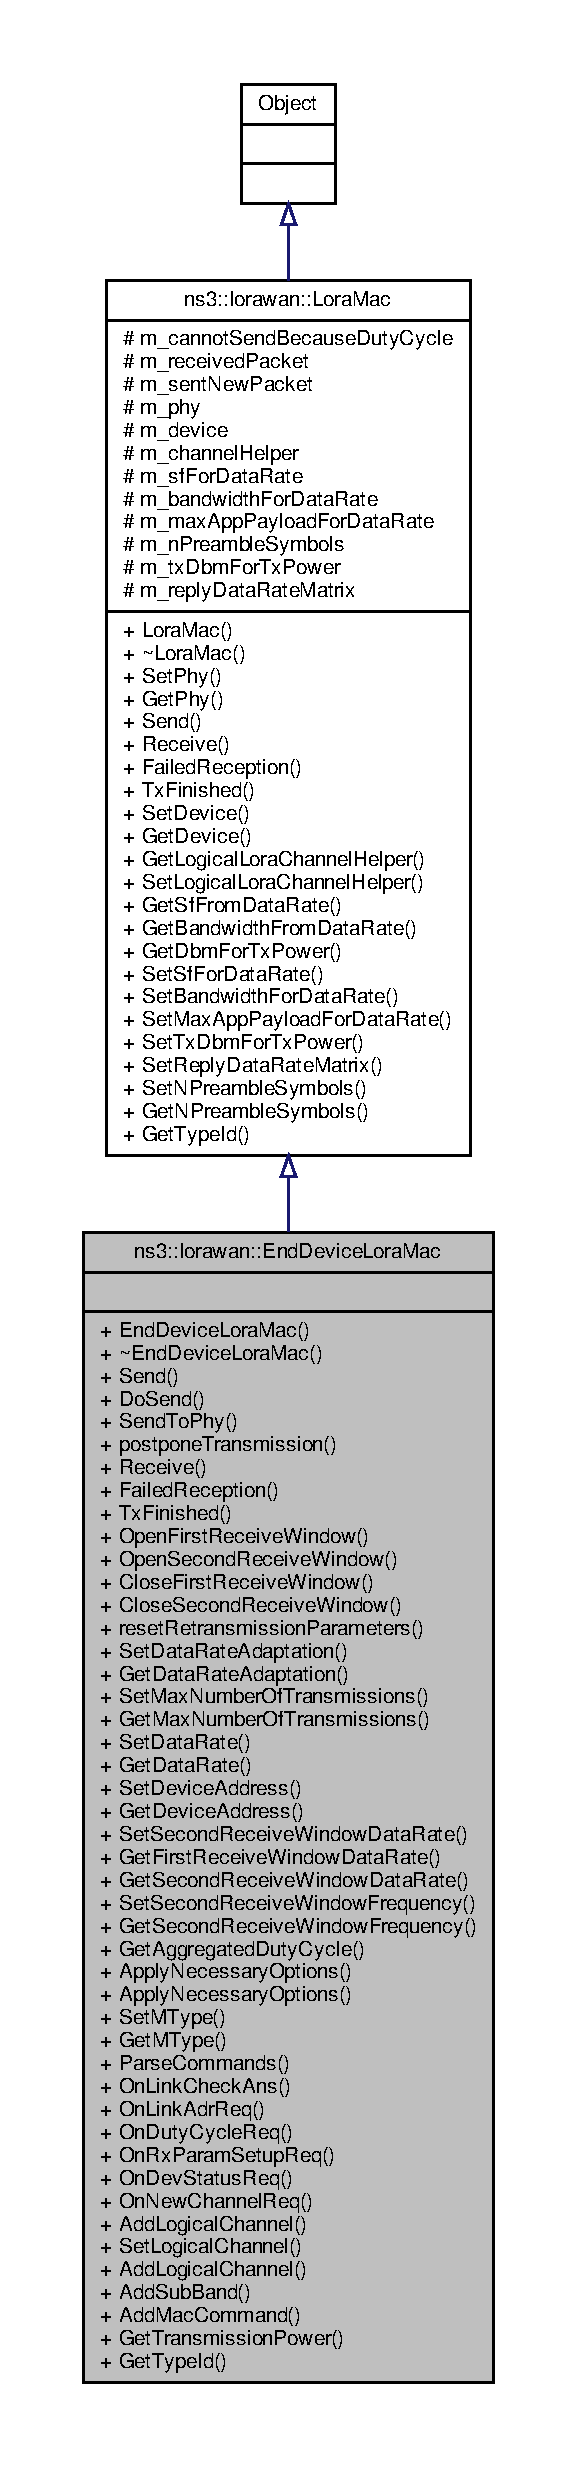
\includegraphics[height=550pt]{classns3_1_1lorawan_1_1EndDeviceLoraMac__inherit__graph}
\end{center}
\end{figure}


Collaboration diagram for ns3\+:\+:lorawan\+:\+:End\+Device\+Lora\+Mac\+:
\nopagebreak
\begin{figure}[H]
\begin{center}
\leavevmode
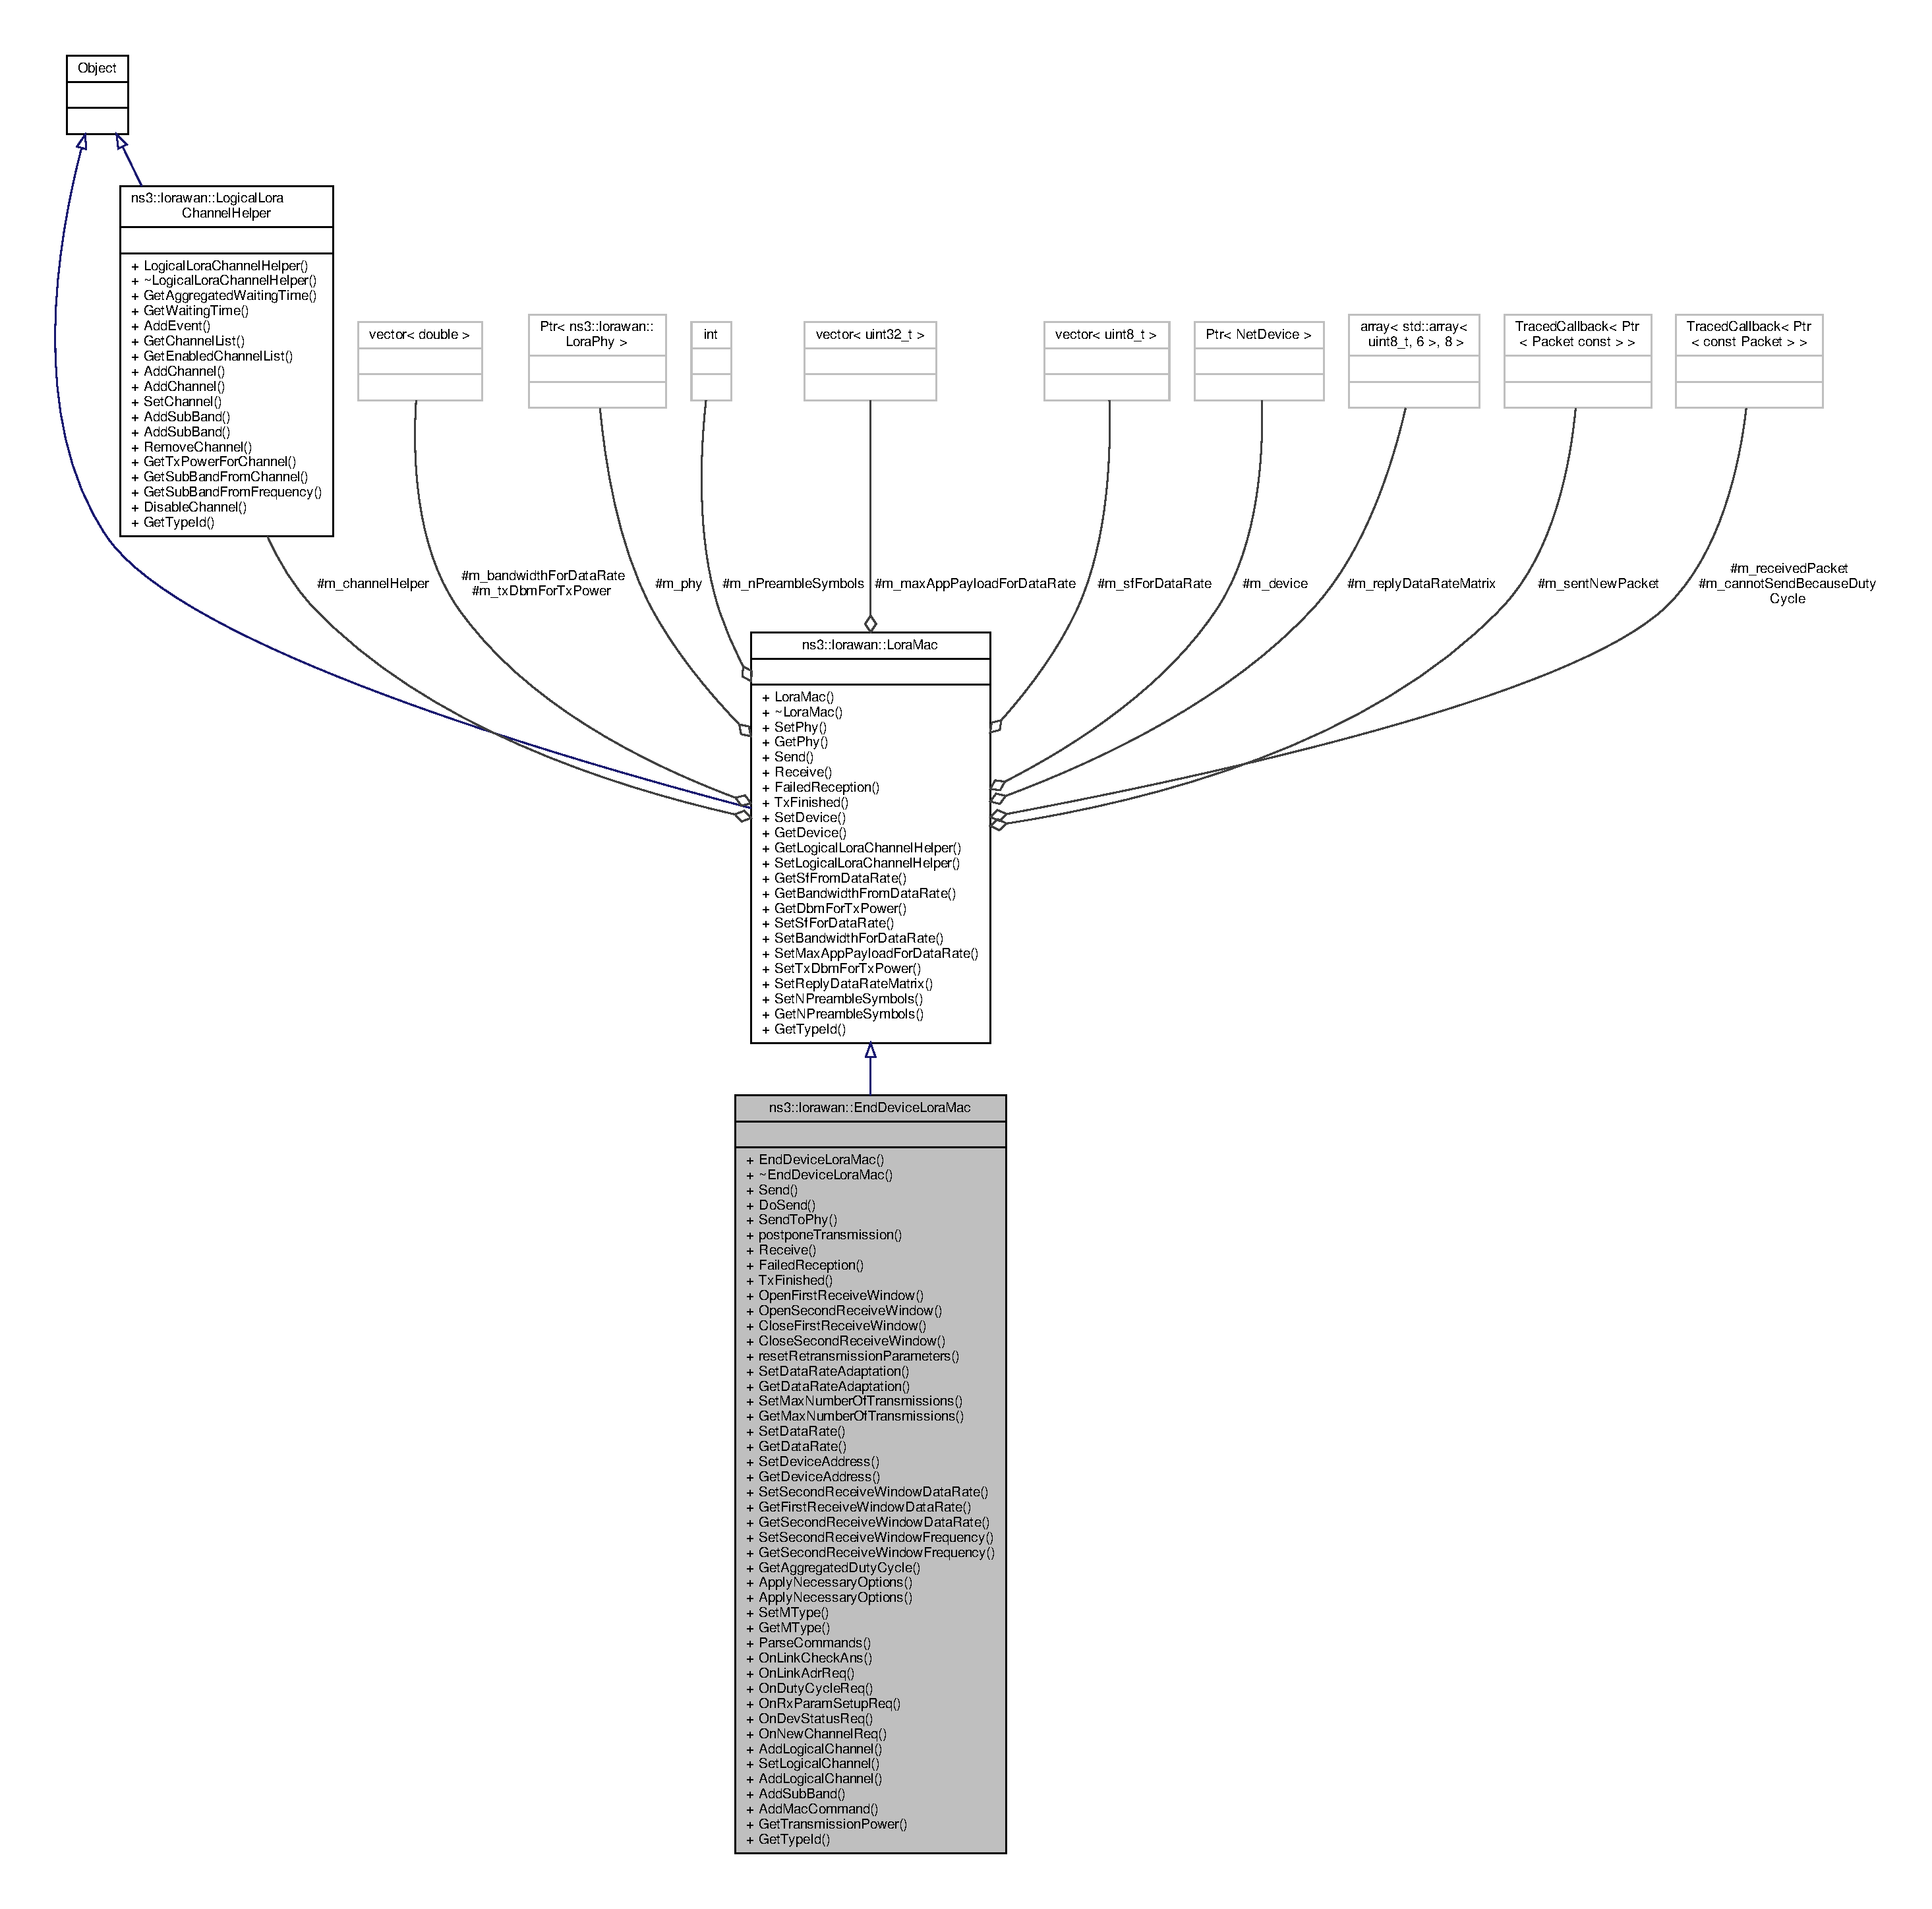
\includegraphics[width=350pt]{classns3_1_1lorawan_1_1EndDeviceLoraMac__coll__graph}
\end{center}
\end{figure}
\subsection*{Public Member Functions}
\begin{DoxyCompactItemize}
\item 
virtual void \hyperlink{classns3_1_1lorawan_1_1EndDeviceLoraMac_a6566cdcccf21b69267215758f36e7ee9}{Send} (Ptr$<$ Packet $>$ packet)
\item 
virtual void \hyperlink{classns3_1_1lorawan_1_1EndDeviceLoraMac_a1e1e4b2c0250f5d37456817f936e5eda}{Do\+Send} (Ptr$<$ Packet $>$ packet)
\item 
virtual void \hyperlink{classns3_1_1lorawan_1_1EndDeviceLoraMac_a4a763f71c529f8557264ea61b7d2b81e}{Send\+To\+Phy} (Ptr$<$ Packet $>$ packet)
\item 
virtual void \hyperlink{classns3_1_1lorawan_1_1EndDeviceLoraMac_a52344bd799bd6c0bc4032b0137f1a1c4}{postpone\+Transmission} (Time next\+Tx\+Delay, Ptr$<$ Packet $>$)
\item 
virtual void \hyperlink{classns3_1_1lorawan_1_1EndDeviceLoraMac_a7bb29a550534c631e2ee7cc3407a2bcd}{Receive} (Ptr$<$ Packet const $>$ packet)
\item 
virtual void \hyperlink{classns3_1_1lorawan_1_1EndDeviceLoraMac_ab1fe806e8a0f5aa3a17fd1c39e831d44}{Failed\+Reception} (Ptr$<$ Packet const $>$ packet)
\item 
void \hyperlink{classns3_1_1lorawan_1_1EndDeviceLoraMac_a939732c613ae14a71c902ade45ee2e40}{Tx\+Finished} (Ptr$<$ const Packet $>$ packet)
\item 
void \hyperlink{classns3_1_1lorawan_1_1EndDeviceLoraMac_a95863dd6763948f579b94ffa6acc6b0c}{Open\+First\+Receive\+Window} (void)
\item 
void \hyperlink{classns3_1_1lorawan_1_1EndDeviceLoraMac_ac7d55666cfe7adc2f159b87543811ba2}{Open\+Second\+Receive\+Window} (void)
\item 
void \hyperlink{classns3_1_1lorawan_1_1EndDeviceLoraMac_ae9ab8ccd648b94b6b9aa7d8c18272274}{Close\+First\+Receive\+Window} (void)
\item 
void \hyperlink{classns3_1_1lorawan_1_1EndDeviceLoraMac_a522179b116be5fe2edd2f4806e00a055}{Close\+Second\+Receive\+Window} (void)
\item 
virtual void \hyperlink{classns3_1_1lorawan_1_1EndDeviceLoraMac_aaa243098bbaf100c7880d2ff9d936ac3}{reset\+Retransmission\+Parameters} ()
\item 
void \hyperlink{classns3_1_1lorawan_1_1EndDeviceLoraMac_a32175f77b6b6386f5092a4800e6c41bb}{Set\+Data\+Rate\+Adaptation} (bool adapt)
\item 
bool \hyperlink{classns3_1_1lorawan_1_1EndDeviceLoraMac_aa3b3b1eff843d141de27ad73e42d1d51}{Get\+Data\+Rate\+Adaptation} (void)
\item 
void \hyperlink{classns3_1_1lorawan_1_1EndDeviceLoraMac_ad9ccf221f703b83cb1a0c0a7b07de03b}{Set\+Max\+Number\+Of\+Transmissions} (uint8\+\_\+t max\+Numb\+Tx)
\item 
uint8\+\_\+t \hyperlink{classns3_1_1lorawan_1_1EndDeviceLoraMac_a693be5d8132d489a1aa099029ad133ab}{Get\+Max\+Number\+Of\+Transmissions} (void)
\item 
void \hyperlink{classns3_1_1lorawan_1_1EndDeviceLoraMac_a4c62f5aba7104a6935e74594d064028e}{Set\+Data\+Rate} (uint8\+\_\+t data\+Rate)
\item 
uint8\+\_\+t \hyperlink{classns3_1_1lorawan_1_1EndDeviceLoraMac_a542adf7ed65bee26b4d43ed49f54a3f4}{Get\+Data\+Rate} (void)
\item 
void \hyperlink{classns3_1_1lorawan_1_1EndDeviceLoraMac_a304aa4040eefef152a13a8496a611404}{Set\+Device\+Address} (\hyperlink{classns3_1_1lorawan_1_1LoraDeviceAddress}{Lora\+Device\+Address} address)
\item 
\hyperlink{classns3_1_1lorawan_1_1LoraDeviceAddress}{Lora\+Device\+Address} \hyperlink{classns3_1_1lorawan_1_1EndDeviceLoraMac_a27064ed2de9f1a8eebc0f57e042f24a1}{Get\+Device\+Address} (void)
\item 
void \hyperlink{classns3_1_1lorawan_1_1EndDeviceLoraMac_a1665b5bad99ef1ee5ca726e8efb6736d}{Set\+Second\+Receive\+Window\+Data\+Rate} (uint8\+\_\+t data\+Rate)
\item 
uint8\+\_\+t \hyperlink{classns3_1_1lorawan_1_1EndDeviceLoraMac_a7156019e4178af699bd4cc328b598995}{Get\+First\+Receive\+Window\+Data\+Rate} (void)
\item 
uint8\+\_\+t \hyperlink{classns3_1_1lorawan_1_1EndDeviceLoraMac_aa4b004ed8d0a79905ad95687a93e4c4f}{Get\+Second\+Receive\+Window\+Data\+Rate} (void)
\item 
void \hyperlink{classns3_1_1lorawan_1_1EndDeviceLoraMac_a366ff7099a3ae9afb64c9ca6be521c55}{Set\+Second\+Receive\+Window\+Frequency} (double frequency\+M\+Hz)
\item 
double \hyperlink{classns3_1_1lorawan_1_1EndDeviceLoraMac_af5ba5257abb97817dc4f5266d7611833}{Get\+Second\+Receive\+Window\+Frequency} (void)
\item 
double \hyperlink{classns3_1_1lorawan_1_1EndDeviceLoraMac_ae974b8539199bbc493ba5436d1689860}{Get\+Aggregated\+Duty\+Cycle} (void)
\item 
void \hyperlink{classns3_1_1lorawan_1_1EndDeviceLoraMac_ac6144c66067865ab2f10a10fb3373139}{Apply\+Necessary\+Options} (\hyperlink{classns3_1_1lorawan_1_1LoraFrameHeader}{Lora\+Frame\+Header} \&frame\+Header)
\item 
void \hyperlink{classns3_1_1lorawan_1_1EndDeviceLoraMac_a5bc2f6e706621d52e20da44af99ba8e6}{Apply\+Necessary\+Options} (\hyperlink{classns3_1_1lorawan_1_1LoraMacHeader}{Lora\+Mac\+Header} \&mac\+Header)
\item 
void \hyperlink{classns3_1_1lorawan_1_1EndDeviceLoraMac_ac1142dacc77786c0e83d364c30a61900}{Set\+M\+Type} (\hyperlink{classns3_1_1lorawan_1_1LoraMacHeader_afd050ac67eab24871452323799e07e94}{Lora\+Mac\+Header\+::\+M\+Type} m\+Type)
\item 
\hyperlink{classns3_1_1lorawan_1_1LoraMacHeader_afd050ac67eab24871452323799e07e94}{Lora\+Mac\+Header\+::\+M\+Type} \hyperlink{classns3_1_1lorawan_1_1EndDeviceLoraMac_a71370a25ca078710f64b80e5d6316263}{Get\+M\+Type} (void)
\item 
void \hyperlink{classns3_1_1lorawan_1_1EndDeviceLoraMac_a7ca5d196ac64e1dfdddd8738f8d1cfbb}{Parse\+Commands} (\hyperlink{classns3_1_1lorawan_1_1LoraFrameHeader}{Lora\+Frame\+Header} frame\+Header)
\item 
void \hyperlink{classns3_1_1lorawan_1_1EndDeviceLoraMac_acab0de0c72baf1bd80108b82dd953874}{On\+Link\+Check\+Ans} (uint8\+\_\+t margin, uint8\+\_\+t gw\+Cnt)
\item 
void \hyperlink{classns3_1_1lorawan_1_1EndDeviceLoraMac_a0564c4a7980faf203e20ef78d847b66f}{On\+Link\+Adr\+Req} (uint8\+\_\+t data\+Rate, uint8\+\_\+t tx\+Power, std\+::list$<$ int $>$ enabled\+Channels, int repetitions)
\item 
void \hyperlink{classns3_1_1lorawan_1_1EndDeviceLoraMac_ab00b3b62618312878a3e231d08e011d9}{On\+Duty\+Cycle\+Req} (double duty\+Cycle)
\item 
void \hyperlink{classns3_1_1lorawan_1_1EndDeviceLoraMac_abe423a1fb1a82c2264f362670197eb55}{On\+Rx\+Param\+Setup\+Req} (uint8\+\_\+t rx1\+Dr\+Offset, uint8\+\_\+t rx2\+Data\+Rate, double frequency)
\item 
void \hyperlink{classns3_1_1lorawan_1_1EndDeviceLoraMac_a46ee940bbd3311012614b352761158df}{On\+Dev\+Status\+Req} (void)
\item 
void \hyperlink{classns3_1_1lorawan_1_1EndDeviceLoraMac_a394c957d5dd4c8e35e431dd26d276995}{On\+New\+Channel\+Req} (uint8\+\_\+t ch\+Index, double frequency, uint8\+\_\+t min\+Data\+Rate, uint8\+\_\+t max\+Data\+Rate)
\item 
void \hyperlink{classns3_1_1lorawan_1_1EndDeviceLoraMac_a35d02edc0a4259d5a6a165579a08391b}{Add\+Logical\+Channel} (double frequency)
\item 
void \hyperlink{classns3_1_1lorawan_1_1EndDeviceLoraMac_aad7490b330e71e9d664dd278b2c294b6}{Set\+Logical\+Channel} (uint8\+\_\+t ch\+Index, double frequency, uint8\+\_\+t min\+Data\+Rate, uint8\+\_\+t max\+Data\+Rate)
\item 
void \hyperlink{classns3_1_1lorawan_1_1EndDeviceLoraMac_a024d4b672a6b0fd3e8e6d3087dac7d6a}{Add\+Logical\+Channel} (Ptr$<$ \hyperlink{classns3_1_1lorawan_1_1LogicalLoraChannel}{Logical\+Lora\+Channel} $>$ logical\+Channel)
\item 
void \hyperlink{classns3_1_1lorawan_1_1EndDeviceLoraMac_a0ec4f0dc1b5fe2feb17125f5d3fbb3b9}{Add\+Sub\+Band} (double start\+Frequency, double end\+Frequency, double duty\+Cycle, double max\+Tx\+Power\+Dbm)
\item 
void \hyperlink{classns3_1_1lorawan_1_1EndDeviceLoraMac_a9c830a6ebb06b450727f7c226e0e2c01}{Add\+Mac\+Command} (Ptr$<$ \hyperlink{classns3_1_1lorawan_1_1MacCommand}{Mac\+Command} $>$ mac\+Command)
\item 
\mbox{\Hypertarget{classns3_1_1lorawan_1_1EndDeviceLoraMac_aca59855646351574a5c8bf593615c375}\label{classns3_1_1lorawan_1_1EndDeviceLoraMac_aca59855646351574a5c8bf593615c375}} 
uint8\+\_\+t {\bfseries Get\+Transmission\+Power} (void)
\end{DoxyCompactItemize}
\subsection*{Static Public Member Functions}
\begin{DoxyCompactItemize}
\item 
\mbox{\Hypertarget{classns3_1_1lorawan_1_1EndDeviceLoraMac_af7ddbf9c251ea22cae05c6dd70da5a9f}\label{classns3_1_1lorawan_1_1EndDeviceLoraMac_af7ddbf9c251ea22cae05c6dd70da5a9f}} 
static Type\+Id {\bfseries Get\+Type\+Id} (void)
\end{DoxyCompactItemize}
\subsection*{Additional Inherited Members}


\subsection{Detailed Description}
Class representing the M\+AC layer of a Lo\+Ra\+W\+AN device. 

\subsection{Member Function Documentation}
\mbox{\Hypertarget{classns3_1_1lorawan_1_1EndDeviceLoraMac_a35d02edc0a4259d5a6a165579a08391b}\label{classns3_1_1lorawan_1_1EndDeviceLoraMac_a35d02edc0a4259d5a6a165579a08391b}} 
\index{ns3\+::lorawan\+::\+End\+Device\+Lora\+Mac@{ns3\+::lorawan\+::\+End\+Device\+Lora\+Mac}!Add\+Logical\+Channel@{Add\+Logical\+Channel}}
\index{Add\+Logical\+Channel@{Add\+Logical\+Channel}!ns3\+::lorawan\+::\+End\+Device\+Lora\+Mac@{ns3\+::lorawan\+::\+End\+Device\+Lora\+Mac}}
\subsubsection{\texorpdfstring{Add\+Logical\+Channel()}{AddLogicalChannel()}\hspace{0.1cm}{\footnotesize\ttfamily [1/2]}}
{\footnotesize\ttfamily void ns3\+::lorawan\+::\+End\+Device\+Lora\+Mac\+::\+Add\+Logical\+Channel (\begin{DoxyParamCaption}\item[{double}]{frequency }\end{DoxyParamCaption})}

Add a logical channel to the helper.


\begin{DoxyParams}{Parameters}
{\em frequency} & The channel\textquotesingle{}s center frequency. \\
\hline
\end{DoxyParams}
\mbox{\Hypertarget{classns3_1_1lorawan_1_1EndDeviceLoraMac_a024d4b672a6b0fd3e8e6d3087dac7d6a}\label{classns3_1_1lorawan_1_1EndDeviceLoraMac_a024d4b672a6b0fd3e8e6d3087dac7d6a}} 
\index{ns3\+::lorawan\+::\+End\+Device\+Lora\+Mac@{ns3\+::lorawan\+::\+End\+Device\+Lora\+Mac}!Add\+Logical\+Channel@{Add\+Logical\+Channel}}
\index{Add\+Logical\+Channel@{Add\+Logical\+Channel}!ns3\+::lorawan\+::\+End\+Device\+Lora\+Mac@{ns3\+::lorawan\+::\+End\+Device\+Lora\+Mac}}
\subsubsection{\texorpdfstring{Add\+Logical\+Channel()}{AddLogicalChannel()}\hspace{0.1cm}{\footnotesize\ttfamily [2/2]}}
{\footnotesize\ttfamily void ns3\+::lorawan\+::\+End\+Device\+Lora\+Mac\+::\+Add\+Logical\+Channel (\begin{DoxyParamCaption}\item[{Ptr$<$ \hyperlink{classns3_1_1lorawan_1_1LogicalLoraChannel}{Logical\+Lora\+Channel} $>$}]{logical\+Channel }\end{DoxyParamCaption})}

Add a logical channel to the helper.


\begin{DoxyParams}{Parameters}
{\em frequency} & The channel\textquotesingle{}s center frequency. \\
\hline
\end{DoxyParams}
\mbox{\Hypertarget{classns3_1_1lorawan_1_1EndDeviceLoraMac_a9c830a6ebb06b450727f7c226e0e2c01}\label{classns3_1_1lorawan_1_1EndDeviceLoraMac_a9c830a6ebb06b450727f7c226e0e2c01}} 
\index{ns3\+::lorawan\+::\+End\+Device\+Lora\+Mac@{ns3\+::lorawan\+::\+End\+Device\+Lora\+Mac}!Add\+Mac\+Command@{Add\+Mac\+Command}}
\index{Add\+Mac\+Command@{Add\+Mac\+Command}!ns3\+::lorawan\+::\+End\+Device\+Lora\+Mac@{ns3\+::lorawan\+::\+End\+Device\+Lora\+Mac}}
\subsubsection{\texorpdfstring{Add\+Mac\+Command()}{AddMacCommand()}}
{\footnotesize\ttfamily void ns3\+::lorawan\+::\+End\+Device\+Lora\+Mac\+::\+Add\+Mac\+Command (\begin{DoxyParamCaption}\item[{Ptr$<$ \hyperlink{classns3_1_1lorawan_1_1MacCommand}{Mac\+Command} $>$}]{mac\+Command }\end{DoxyParamCaption})}

Add a M\+AC command to the list of those that will be sent out in the next packet. \mbox{\Hypertarget{classns3_1_1lorawan_1_1EndDeviceLoraMac_a0ec4f0dc1b5fe2feb17125f5d3fbb3b9}\label{classns3_1_1lorawan_1_1EndDeviceLoraMac_a0ec4f0dc1b5fe2feb17125f5d3fbb3b9}} 
\index{ns3\+::lorawan\+::\+End\+Device\+Lora\+Mac@{ns3\+::lorawan\+::\+End\+Device\+Lora\+Mac}!Add\+Sub\+Band@{Add\+Sub\+Band}}
\index{Add\+Sub\+Band@{Add\+Sub\+Band}!ns3\+::lorawan\+::\+End\+Device\+Lora\+Mac@{ns3\+::lorawan\+::\+End\+Device\+Lora\+Mac}}
\subsubsection{\texorpdfstring{Add\+Sub\+Band()}{AddSubBand()}}
{\footnotesize\ttfamily void ns3\+::lorawan\+::\+End\+Device\+Lora\+Mac\+::\+Add\+Sub\+Band (\begin{DoxyParamCaption}\item[{double}]{start\+Frequency,  }\item[{double}]{end\+Frequency,  }\item[{double}]{duty\+Cycle,  }\item[{double}]{max\+Tx\+Power\+Dbm }\end{DoxyParamCaption})}

Add a subband to the logical channel helper.


\begin{DoxyParams}{Parameters}
{\em start\+Frequency} & The \hyperlink{classns3_1_1lorawan_1_1SubBand}{Sub\+Band}\textquotesingle{}s lowest frequency. \\
\hline
{\em end\+Frequency} & The \hyperlink{classns3_1_1lorawan_1_1SubBand}{Sub\+Band}\textquotesingle{}s highest frequency. \\
\hline
{\em duty\+Cycle} & The \hyperlink{classns3_1_1lorawan_1_1SubBand}{Sub\+Band}\textquotesingle{}s duty cycle, in fraction form. \\
\hline
{\em max\+Tx\+Power\+Dbm} & The maximum transmission power allowed on the \hyperlink{classns3_1_1lorawan_1_1SubBand}{Sub\+Band}. \\
\hline
\end{DoxyParams}
\mbox{\Hypertarget{classns3_1_1lorawan_1_1EndDeviceLoraMac_ac6144c66067865ab2f10a10fb3373139}\label{classns3_1_1lorawan_1_1EndDeviceLoraMac_ac6144c66067865ab2f10a10fb3373139}} 
\index{ns3\+::lorawan\+::\+End\+Device\+Lora\+Mac@{ns3\+::lorawan\+::\+End\+Device\+Lora\+Mac}!Apply\+Necessary\+Options@{Apply\+Necessary\+Options}}
\index{Apply\+Necessary\+Options@{Apply\+Necessary\+Options}!ns3\+::lorawan\+::\+End\+Device\+Lora\+Mac@{ns3\+::lorawan\+::\+End\+Device\+Lora\+Mac}}
\subsubsection{\texorpdfstring{Apply\+Necessary\+Options()}{ApplyNecessaryOptions()}\hspace{0.1cm}{\footnotesize\ttfamily [1/2]}}
{\footnotesize\ttfamily void ns3\+::lorawan\+::\+End\+Device\+Lora\+Mac\+::\+Apply\+Necessary\+Options (\begin{DoxyParamCaption}\item[{\hyperlink{classns3_1_1lorawan_1_1LoraFrameHeader}{Lora\+Frame\+Header} \&}]{frame\+Header }\end{DoxyParamCaption})}

Add the necessary options and M\+AC commands to the \hyperlink{classns3_1_1lorawan_1_1LoraFrameHeader}{Lora\+Frame\+Header}.


\begin{DoxyParams}{Parameters}
{\em frame\+Header} & The frame header on which to apply the options. \\
\hline
\end{DoxyParams}
\mbox{\Hypertarget{classns3_1_1lorawan_1_1EndDeviceLoraMac_a5bc2f6e706621d52e20da44af99ba8e6}\label{classns3_1_1lorawan_1_1EndDeviceLoraMac_a5bc2f6e706621d52e20da44af99ba8e6}} 
\index{ns3\+::lorawan\+::\+End\+Device\+Lora\+Mac@{ns3\+::lorawan\+::\+End\+Device\+Lora\+Mac}!Apply\+Necessary\+Options@{Apply\+Necessary\+Options}}
\index{Apply\+Necessary\+Options@{Apply\+Necessary\+Options}!ns3\+::lorawan\+::\+End\+Device\+Lora\+Mac@{ns3\+::lorawan\+::\+End\+Device\+Lora\+Mac}}
\subsubsection{\texorpdfstring{Apply\+Necessary\+Options()}{ApplyNecessaryOptions()}\hspace{0.1cm}{\footnotesize\ttfamily [2/2]}}
{\footnotesize\ttfamily void ns3\+::lorawan\+::\+End\+Device\+Lora\+Mac\+::\+Apply\+Necessary\+Options (\begin{DoxyParamCaption}\item[{\hyperlink{classns3_1_1lorawan_1_1LoraMacHeader}{Lora\+Mac\+Header} \&}]{mac\+Header }\end{DoxyParamCaption})}

Add the necessary options and M\+AC commands to the \hyperlink{classns3_1_1lorawan_1_1LoraMacHeader}{Lora\+Mac\+Header}.


\begin{DoxyParams}{Parameters}
{\em mac\+Header} & The mac header on which to apply the options. \\
\hline
\end{DoxyParams}
\mbox{\Hypertarget{classns3_1_1lorawan_1_1EndDeviceLoraMac_ae9ab8ccd648b94b6b9aa7d8c18272274}\label{classns3_1_1lorawan_1_1EndDeviceLoraMac_ae9ab8ccd648b94b6b9aa7d8c18272274}} 
\index{ns3\+::lorawan\+::\+End\+Device\+Lora\+Mac@{ns3\+::lorawan\+::\+End\+Device\+Lora\+Mac}!Close\+First\+Receive\+Window@{Close\+First\+Receive\+Window}}
\index{Close\+First\+Receive\+Window@{Close\+First\+Receive\+Window}!ns3\+::lorawan\+::\+End\+Device\+Lora\+Mac@{ns3\+::lorawan\+::\+End\+Device\+Lora\+Mac}}
\subsubsection{\texorpdfstring{Close\+First\+Receive\+Window()}{CloseFirstReceiveWindow()}}
{\footnotesize\ttfamily void ns3\+::lorawan\+::\+End\+Device\+Lora\+Mac\+::\+Close\+First\+Receive\+Window (\begin{DoxyParamCaption}\item[{void}]{ }\end{DoxyParamCaption})}

Perform operations needed to close the first receive window. \mbox{\Hypertarget{classns3_1_1lorawan_1_1EndDeviceLoraMac_a522179b116be5fe2edd2f4806e00a055}\label{classns3_1_1lorawan_1_1EndDeviceLoraMac_a522179b116be5fe2edd2f4806e00a055}} 
\index{ns3\+::lorawan\+::\+End\+Device\+Lora\+Mac@{ns3\+::lorawan\+::\+End\+Device\+Lora\+Mac}!Close\+Second\+Receive\+Window@{Close\+Second\+Receive\+Window}}
\index{Close\+Second\+Receive\+Window@{Close\+Second\+Receive\+Window}!ns3\+::lorawan\+::\+End\+Device\+Lora\+Mac@{ns3\+::lorawan\+::\+End\+Device\+Lora\+Mac}}
\subsubsection{\texorpdfstring{Close\+Second\+Receive\+Window()}{CloseSecondReceiveWindow()}}
{\footnotesize\ttfamily void ns3\+::lorawan\+::\+End\+Device\+Lora\+Mac\+::\+Close\+Second\+Receive\+Window (\begin{DoxyParamCaption}\item[{void}]{ }\end{DoxyParamCaption})}

Perform operations needed to close the second receive window. \mbox{\Hypertarget{classns3_1_1lorawan_1_1EndDeviceLoraMac_a1e1e4b2c0250f5d37456817f936e5eda}\label{classns3_1_1lorawan_1_1EndDeviceLoraMac_a1e1e4b2c0250f5d37456817f936e5eda}} 
\index{ns3\+::lorawan\+::\+End\+Device\+Lora\+Mac@{ns3\+::lorawan\+::\+End\+Device\+Lora\+Mac}!Do\+Send@{Do\+Send}}
\index{Do\+Send@{Do\+Send}!ns3\+::lorawan\+::\+End\+Device\+Lora\+Mac@{ns3\+::lorawan\+::\+End\+Device\+Lora\+Mac}}
\subsubsection{\texorpdfstring{Do\+Send()}{DoSend()}}
{\footnotesize\ttfamily void ns3\+::lorawan\+::\+End\+Device\+Lora\+Mac\+::\+Do\+Send (\begin{DoxyParamCaption}\item[{Ptr$<$ Packet $>$}]{packet }\end{DoxyParamCaption})\hspace{0.3cm}{\ttfamily [virtual]}}

Checking if we are performing the transmission of a new packet or a retransmission, and call Send\+To\+Phy function.


\begin{DoxyParams}{Parameters}
{\em packet} & the packet to send \\
\hline
\end{DoxyParams}
\mbox{\Hypertarget{classns3_1_1lorawan_1_1EndDeviceLoraMac_ab1fe806e8a0f5aa3a17fd1c39e831d44}\label{classns3_1_1lorawan_1_1EndDeviceLoraMac_ab1fe806e8a0f5aa3a17fd1c39e831d44}} 
\index{ns3\+::lorawan\+::\+End\+Device\+Lora\+Mac@{ns3\+::lorawan\+::\+End\+Device\+Lora\+Mac}!Failed\+Reception@{Failed\+Reception}}
\index{Failed\+Reception@{Failed\+Reception}!ns3\+::lorawan\+::\+End\+Device\+Lora\+Mac@{ns3\+::lorawan\+::\+End\+Device\+Lora\+Mac}}
\subsubsection{\texorpdfstring{Failed\+Reception()}{FailedReception()}}
{\footnotesize\ttfamily void ns3\+::lorawan\+::\+End\+Device\+Lora\+Mac\+::\+Failed\+Reception (\begin{DoxyParamCaption}\item[{Ptr$<$ Packet const $>$}]{packet }\end{DoxyParamCaption})\hspace{0.3cm}{\ttfamily [virtual]}}

Function called by lower layers to inform this layer that reception of a packet we were locked on failed.


\begin{DoxyParams}{Parameters}
{\em packet} & the packet we failed to receive \\
\hline
\end{DoxyParams}


Implements \hyperlink{classns3_1_1lorawan_1_1LoraMac_afcd55472bbfa299c4d0239d5fa9957e3}{ns3\+::lorawan\+::\+Lora\+Mac}.

\mbox{\Hypertarget{classns3_1_1lorawan_1_1EndDeviceLoraMac_ae974b8539199bbc493ba5436d1689860}\label{classns3_1_1lorawan_1_1EndDeviceLoraMac_ae974b8539199bbc493ba5436d1689860}} 
\index{ns3\+::lorawan\+::\+End\+Device\+Lora\+Mac@{ns3\+::lorawan\+::\+End\+Device\+Lora\+Mac}!Get\+Aggregated\+Duty\+Cycle@{Get\+Aggregated\+Duty\+Cycle}}
\index{Get\+Aggregated\+Duty\+Cycle@{Get\+Aggregated\+Duty\+Cycle}!ns3\+::lorawan\+::\+End\+Device\+Lora\+Mac@{ns3\+::lorawan\+::\+End\+Device\+Lora\+Mac}}
\subsubsection{\texorpdfstring{Get\+Aggregated\+Duty\+Cycle()}{GetAggregatedDutyCycle()}}
{\footnotesize\ttfamily double ns3\+::lorawan\+::\+End\+Device\+Lora\+Mac\+::\+Get\+Aggregated\+Duty\+Cycle (\begin{DoxyParamCaption}\item[{void}]{ }\end{DoxyParamCaption})}

Set a value for the R\+X1\+D\+R\+Offset parameter.

This value decides the offset to use when deciding the Data\+Rate of the downlink transmission during the first receive window from the reply\+Data\+Rate\+Matrix.


\begin{DoxyParams}{Parameters}
{\em rx1\+Dr\+Offset} & The value to set for the offset. Get the value of the R\+X1\+D\+R\+Offset parameter.\\
\hline
\end{DoxyParams}
\begin{DoxyReturn}{Returns}
The value of the R\+X1\+D\+R\+Offset parameter. Get the aggregated duty cycle.

A time instance containing the aggregated duty cycle in fractional form. 
\end{DoxyReturn}
\mbox{\Hypertarget{classns3_1_1lorawan_1_1EndDeviceLoraMac_a542adf7ed65bee26b4d43ed49f54a3f4}\label{classns3_1_1lorawan_1_1EndDeviceLoraMac_a542adf7ed65bee26b4d43ed49f54a3f4}} 
\index{ns3\+::lorawan\+::\+End\+Device\+Lora\+Mac@{ns3\+::lorawan\+::\+End\+Device\+Lora\+Mac}!Get\+Data\+Rate@{Get\+Data\+Rate}}
\index{Get\+Data\+Rate@{Get\+Data\+Rate}!ns3\+::lorawan\+::\+End\+Device\+Lora\+Mac@{ns3\+::lorawan\+::\+End\+Device\+Lora\+Mac}}
\subsubsection{\texorpdfstring{Get\+Data\+Rate()}{GetDataRate()}}
{\footnotesize\ttfamily uint8\+\_\+t ns3\+::lorawan\+::\+End\+Device\+Lora\+Mac\+::\+Get\+Data\+Rate (\begin{DoxyParamCaption}\item[{void}]{ }\end{DoxyParamCaption})}

Get the data rate this end device is set to use.

\begin{DoxyReturn}{Returns}
The data rate this device uses when transmitting. 
\end{DoxyReturn}
\mbox{\Hypertarget{classns3_1_1lorawan_1_1EndDeviceLoraMac_aa3b3b1eff843d141de27ad73e42d1d51}\label{classns3_1_1lorawan_1_1EndDeviceLoraMac_aa3b3b1eff843d141de27ad73e42d1d51}} 
\index{ns3\+::lorawan\+::\+End\+Device\+Lora\+Mac@{ns3\+::lorawan\+::\+End\+Device\+Lora\+Mac}!Get\+Data\+Rate\+Adaptation@{Get\+Data\+Rate\+Adaptation}}
\index{Get\+Data\+Rate\+Adaptation@{Get\+Data\+Rate\+Adaptation}!ns3\+::lorawan\+::\+End\+Device\+Lora\+Mac@{ns3\+::lorawan\+::\+End\+Device\+Lora\+Mac}}
\subsubsection{\texorpdfstring{Get\+Data\+Rate\+Adaptation()}{GetDataRateAdaptation()}}
{\footnotesize\ttfamily bool ns3\+::lorawan\+::\+End\+Device\+Lora\+Mac\+::\+Get\+Data\+Rate\+Adaptation (\begin{DoxyParamCaption}\item[{void}]{ }\end{DoxyParamCaption})}

Get if data rate adaptation is enabled or not. \mbox{\Hypertarget{classns3_1_1lorawan_1_1EndDeviceLoraMac_a27064ed2de9f1a8eebc0f57e042f24a1}\label{classns3_1_1lorawan_1_1EndDeviceLoraMac_a27064ed2de9f1a8eebc0f57e042f24a1}} 
\index{ns3\+::lorawan\+::\+End\+Device\+Lora\+Mac@{ns3\+::lorawan\+::\+End\+Device\+Lora\+Mac}!Get\+Device\+Address@{Get\+Device\+Address}}
\index{Get\+Device\+Address@{Get\+Device\+Address}!ns3\+::lorawan\+::\+End\+Device\+Lora\+Mac@{ns3\+::lorawan\+::\+End\+Device\+Lora\+Mac}}
\subsubsection{\texorpdfstring{Get\+Device\+Address()}{GetDeviceAddress()}}
{\footnotesize\ttfamily \hyperlink{classns3_1_1lorawan_1_1LoraDeviceAddress}{Lora\+Device\+Address} ns3\+::lorawan\+::\+End\+Device\+Lora\+Mac\+::\+Get\+Device\+Address (\begin{DoxyParamCaption}\item[{void}]{ }\end{DoxyParamCaption})}

Get the network address of this device.

\begin{DoxyReturn}{Returns}
This device\textquotesingle{}s address. 
\end{DoxyReturn}
\mbox{\Hypertarget{classns3_1_1lorawan_1_1EndDeviceLoraMac_a7156019e4178af699bd4cc328b598995}\label{classns3_1_1lorawan_1_1EndDeviceLoraMac_a7156019e4178af699bd4cc328b598995}} 
\index{ns3\+::lorawan\+::\+End\+Device\+Lora\+Mac@{ns3\+::lorawan\+::\+End\+Device\+Lora\+Mac}!Get\+First\+Receive\+Window\+Data\+Rate@{Get\+First\+Receive\+Window\+Data\+Rate}}
\index{Get\+First\+Receive\+Window\+Data\+Rate@{Get\+First\+Receive\+Window\+Data\+Rate}!ns3\+::lorawan\+::\+End\+Device\+Lora\+Mac@{ns3\+::lorawan\+::\+End\+Device\+Lora\+Mac}}
\subsubsection{\texorpdfstring{Get\+First\+Receive\+Window\+Data\+Rate()}{GetFirstReceiveWindowDataRate()}}
{\footnotesize\ttfamily uint8\+\_\+t ns3\+::lorawan\+::\+End\+Device\+Lora\+Mac\+::\+Get\+First\+Receive\+Window\+Data\+Rate (\begin{DoxyParamCaption}\item[{void}]{ }\end{DoxyParamCaption})}

Get the Data Rate that will be used in the first receive window.

\begin{DoxyReturn}{Returns}
The Data Rate 
\end{DoxyReturn}
\mbox{\Hypertarget{classns3_1_1lorawan_1_1EndDeviceLoraMac_a693be5d8132d489a1aa099029ad133ab}\label{classns3_1_1lorawan_1_1EndDeviceLoraMac_a693be5d8132d489a1aa099029ad133ab}} 
\index{ns3\+::lorawan\+::\+End\+Device\+Lora\+Mac@{ns3\+::lorawan\+::\+End\+Device\+Lora\+Mac}!Get\+Max\+Number\+Of\+Transmissions@{Get\+Max\+Number\+Of\+Transmissions}}
\index{Get\+Max\+Number\+Of\+Transmissions@{Get\+Max\+Number\+Of\+Transmissions}!ns3\+::lorawan\+::\+End\+Device\+Lora\+Mac@{ns3\+::lorawan\+::\+End\+Device\+Lora\+Mac}}
\subsubsection{\texorpdfstring{Get\+Max\+Number\+Of\+Transmissions()}{GetMaxNumberOfTransmissions()}}
{\footnotesize\ttfamily uint8\+\_\+t ns3\+::lorawan\+::\+End\+Device\+Lora\+Mac\+::\+Get\+Max\+Number\+Of\+Transmissions (\begin{DoxyParamCaption}\item[{void}]{ }\end{DoxyParamCaption})}

Set the maximum number of transmissions allowed. \mbox{\Hypertarget{classns3_1_1lorawan_1_1EndDeviceLoraMac_a71370a25ca078710f64b80e5d6316263}\label{classns3_1_1lorawan_1_1EndDeviceLoraMac_a71370a25ca078710f64b80e5d6316263}} 
\index{ns3\+::lorawan\+::\+End\+Device\+Lora\+Mac@{ns3\+::lorawan\+::\+End\+Device\+Lora\+Mac}!Get\+M\+Type@{Get\+M\+Type}}
\index{Get\+M\+Type@{Get\+M\+Type}!ns3\+::lorawan\+::\+End\+Device\+Lora\+Mac@{ns3\+::lorawan\+::\+End\+Device\+Lora\+Mac}}
\subsubsection{\texorpdfstring{Get\+M\+Type()}{GetMType()}}
{\footnotesize\ttfamily \hyperlink{classns3_1_1lorawan_1_1LoraMacHeader_afd050ac67eab24871452323799e07e94}{Lora\+Mac\+Header\+::\+M\+Type} ns3\+::lorawan\+::\+End\+Device\+Lora\+Mac\+::\+Get\+M\+Type (\begin{DoxyParamCaption}\item[{void}]{ }\end{DoxyParamCaption})}

Get the message type to send when the Send method is called. \mbox{\Hypertarget{classns3_1_1lorawan_1_1EndDeviceLoraMac_aa4b004ed8d0a79905ad95687a93e4c4f}\label{classns3_1_1lorawan_1_1EndDeviceLoraMac_aa4b004ed8d0a79905ad95687a93e4c4f}} 
\index{ns3\+::lorawan\+::\+End\+Device\+Lora\+Mac@{ns3\+::lorawan\+::\+End\+Device\+Lora\+Mac}!Get\+Second\+Receive\+Window\+Data\+Rate@{Get\+Second\+Receive\+Window\+Data\+Rate}}
\index{Get\+Second\+Receive\+Window\+Data\+Rate@{Get\+Second\+Receive\+Window\+Data\+Rate}!ns3\+::lorawan\+::\+End\+Device\+Lora\+Mac@{ns3\+::lorawan\+::\+End\+Device\+Lora\+Mac}}
\subsubsection{\texorpdfstring{Get\+Second\+Receive\+Window\+Data\+Rate()}{GetSecondReceiveWindowDataRate()}}
{\footnotesize\ttfamily uint8\+\_\+t ns3\+::lorawan\+::\+End\+Device\+Lora\+Mac\+::\+Get\+Second\+Receive\+Window\+Data\+Rate (\begin{DoxyParamCaption}\item[{void}]{ }\end{DoxyParamCaption})}

Get the Data Rate that will be used in the second receive window.

\begin{DoxyReturn}{Returns}
The Data Rate 
\end{DoxyReturn}
\mbox{\Hypertarget{classns3_1_1lorawan_1_1EndDeviceLoraMac_af5ba5257abb97817dc4f5266d7611833}\label{classns3_1_1lorawan_1_1EndDeviceLoraMac_af5ba5257abb97817dc4f5266d7611833}} 
\index{ns3\+::lorawan\+::\+End\+Device\+Lora\+Mac@{ns3\+::lorawan\+::\+End\+Device\+Lora\+Mac}!Get\+Second\+Receive\+Window\+Frequency@{Get\+Second\+Receive\+Window\+Frequency}}
\index{Get\+Second\+Receive\+Window\+Frequency@{Get\+Second\+Receive\+Window\+Frequency}!ns3\+::lorawan\+::\+End\+Device\+Lora\+Mac@{ns3\+::lorawan\+::\+End\+Device\+Lora\+Mac}}
\subsubsection{\texorpdfstring{Get\+Second\+Receive\+Window\+Frequency()}{GetSecondReceiveWindowFrequency()}}
{\footnotesize\ttfamily double ns3\+::lorawan\+::\+End\+Device\+Lora\+Mac\+::\+Get\+Second\+Receive\+Window\+Frequency (\begin{DoxyParamCaption}\item[{void}]{ }\end{DoxyParamCaption})}

Get the frequency that is used for the second receive window.

\begin{DoxyReturn}{Returns}
The frequency, in M\+Hz 
\end{DoxyReturn}
\mbox{\Hypertarget{classns3_1_1lorawan_1_1EndDeviceLoraMac_a46ee940bbd3311012614b352761158df}\label{classns3_1_1lorawan_1_1EndDeviceLoraMac_a46ee940bbd3311012614b352761158df}} 
\index{ns3\+::lorawan\+::\+End\+Device\+Lora\+Mac@{ns3\+::lorawan\+::\+End\+Device\+Lora\+Mac}!On\+Dev\+Status\+Req@{On\+Dev\+Status\+Req}}
\index{On\+Dev\+Status\+Req@{On\+Dev\+Status\+Req}!ns3\+::lorawan\+::\+End\+Device\+Lora\+Mac@{ns3\+::lorawan\+::\+End\+Device\+Lora\+Mac}}
\subsubsection{\texorpdfstring{On\+Dev\+Status\+Req()}{OnDevStatusReq()}}
{\footnotesize\ttfamily void ns3\+::lorawan\+::\+End\+Device\+Lora\+Mac\+::\+On\+Dev\+Status\+Req (\begin{DoxyParamCaption}\item[{void}]{ }\end{DoxyParamCaption})}

Perform the actions that need to be taken when receiving a \hyperlink{classns3_1_1lorawan_1_1DevStatusReq}{Dev\+Status\+Req} command. \mbox{\Hypertarget{classns3_1_1lorawan_1_1EndDeviceLoraMac_ab00b3b62618312878a3e231d08e011d9}\label{classns3_1_1lorawan_1_1EndDeviceLoraMac_ab00b3b62618312878a3e231d08e011d9}} 
\index{ns3\+::lorawan\+::\+End\+Device\+Lora\+Mac@{ns3\+::lorawan\+::\+End\+Device\+Lora\+Mac}!On\+Duty\+Cycle\+Req@{On\+Duty\+Cycle\+Req}}
\index{On\+Duty\+Cycle\+Req@{On\+Duty\+Cycle\+Req}!ns3\+::lorawan\+::\+End\+Device\+Lora\+Mac@{ns3\+::lorawan\+::\+End\+Device\+Lora\+Mac}}
\subsubsection{\texorpdfstring{On\+Duty\+Cycle\+Req()}{OnDutyCycleReq()}}
{\footnotesize\ttfamily void ns3\+::lorawan\+::\+End\+Device\+Lora\+Mac\+::\+On\+Duty\+Cycle\+Req (\begin{DoxyParamCaption}\item[{double}]{duty\+Cycle }\end{DoxyParamCaption})}

Perform the actions that need to be taken when receiving a \hyperlink{classns3_1_1lorawan_1_1DutyCycleReq}{Duty\+Cycle\+Req} command.


\begin{DoxyParams}{Parameters}
{\em duty\+Cycle} & The aggregate duty cycle prescribed by the command, in fraction form. \\
\hline
\end{DoxyParams}
\mbox{\Hypertarget{classns3_1_1lorawan_1_1EndDeviceLoraMac_a0564c4a7980faf203e20ef78d847b66f}\label{classns3_1_1lorawan_1_1EndDeviceLoraMac_a0564c4a7980faf203e20ef78d847b66f}} 
\index{ns3\+::lorawan\+::\+End\+Device\+Lora\+Mac@{ns3\+::lorawan\+::\+End\+Device\+Lora\+Mac}!On\+Link\+Adr\+Req@{On\+Link\+Adr\+Req}}
\index{On\+Link\+Adr\+Req@{On\+Link\+Adr\+Req}!ns3\+::lorawan\+::\+End\+Device\+Lora\+Mac@{ns3\+::lorawan\+::\+End\+Device\+Lora\+Mac}}
\subsubsection{\texorpdfstring{On\+Link\+Adr\+Req()}{OnLinkAdrReq()}}
{\footnotesize\ttfamily void ns3\+::lorawan\+::\+End\+Device\+Lora\+Mac\+::\+On\+Link\+Adr\+Req (\begin{DoxyParamCaption}\item[{uint8\+\_\+t}]{data\+Rate,  }\item[{uint8\+\_\+t}]{tx\+Power,  }\item[{std\+::list$<$ int $>$}]{enabled\+Channels,  }\item[{int}]{repetitions }\end{DoxyParamCaption})}

Perform the actions that need to be taken when receiving a \hyperlink{classns3_1_1lorawan_1_1LinkAdrReq}{Link\+Adr\+Req} command.


\begin{DoxyParams}{Parameters}
{\em data\+Rate} & The data rate value of the command. \\
\hline
{\em tx\+Power} & The transmission power value of the command. \\
\hline
{\em enabled\+Channels} & A list of the enabled channels. \\
\hline
{\em repetitions} & The number of repetitions prescribed by the command. \\
\hline
\end{DoxyParams}
\mbox{\Hypertarget{classns3_1_1lorawan_1_1EndDeviceLoraMac_acab0de0c72baf1bd80108b82dd953874}\label{classns3_1_1lorawan_1_1EndDeviceLoraMac_acab0de0c72baf1bd80108b82dd953874}} 
\index{ns3\+::lorawan\+::\+End\+Device\+Lora\+Mac@{ns3\+::lorawan\+::\+End\+Device\+Lora\+Mac}!On\+Link\+Check\+Ans@{On\+Link\+Check\+Ans}}
\index{On\+Link\+Check\+Ans@{On\+Link\+Check\+Ans}!ns3\+::lorawan\+::\+End\+Device\+Lora\+Mac@{ns3\+::lorawan\+::\+End\+Device\+Lora\+Mac}}
\subsubsection{\texorpdfstring{On\+Link\+Check\+Ans()}{OnLinkCheckAns()}}
{\footnotesize\ttfamily void ns3\+::lorawan\+::\+End\+Device\+Lora\+Mac\+::\+On\+Link\+Check\+Ans (\begin{DoxyParamCaption}\item[{uint8\+\_\+t}]{margin,  }\item[{uint8\+\_\+t}]{gw\+Cnt }\end{DoxyParamCaption})}

Perform the actions that need to be taken when receiving a \hyperlink{classns3_1_1lorawan_1_1LinkCheckAns}{Link\+Check\+Ans} command.


\begin{DoxyParams}{Parameters}
{\em margin} & The margin value of the command. \\
\hline
{\em gw\+Cnt} & The gateway count value of the command. \\
\hline
\end{DoxyParams}
\mbox{\Hypertarget{classns3_1_1lorawan_1_1EndDeviceLoraMac_a394c957d5dd4c8e35e431dd26d276995}\label{classns3_1_1lorawan_1_1EndDeviceLoraMac_a394c957d5dd4c8e35e431dd26d276995}} 
\index{ns3\+::lorawan\+::\+End\+Device\+Lora\+Mac@{ns3\+::lorawan\+::\+End\+Device\+Lora\+Mac}!On\+New\+Channel\+Req@{On\+New\+Channel\+Req}}
\index{On\+New\+Channel\+Req@{On\+New\+Channel\+Req}!ns3\+::lorawan\+::\+End\+Device\+Lora\+Mac@{ns3\+::lorawan\+::\+End\+Device\+Lora\+Mac}}
\subsubsection{\texorpdfstring{On\+New\+Channel\+Req()}{OnNewChannelReq()}}
{\footnotesize\ttfamily void ns3\+::lorawan\+::\+End\+Device\+Lora\+Mac\+::\+On\+New\+Channel\+Req (\begin{DoxyParamCaption}\item[{uint8\+\_\+t}]{ch\+Index,  }\item[{double}]{frequency,  }\item[{uint8\+\_\+t}]{min\+Data\+Rate,  }\item[{uint8\+\_\+t}]{max\+Data\+Rate }\end{DoxyParamCaption})}

Perform the actions that need to be taken when receiving a \hyperlink{classns3_1_1lorawan_1_1NewChannelReq}{New\+Channel\+Req} command. \mbox{\Hypertarget{classns3_1_1lorawan_1_1EndDeviceLoraMac_abe423a1fb1a82c2264f362670197eb55}\label{classns3_1_1lorawan_1_1EndDeviceLoraMac_abe423a1fb1a82c2264f362670197eb55}} 
\index{ns3\+::lorawan\+::\+End\+Device\+Lora\+Mac@{ns3\+::lorawan\+::\+End\+Device\+Lora\+Mac}!On\+Rx\+Param\+Setup\+Req@{On\+Rx\+Param\+Setup\+Req}}
\index{On\+Rx\+Param\+Setup\+Req@{On\+Rx\+Param\+Setup\+Req}!ns3\+::lorawan\+::\+End\+Device\+Lora\+Mac@{ns3\+::lorawan\+::\+End\+Device\+Lora\+Mac}}
\subsubsection{\texorpdfstring{On\+Rx\+Param\+Setup\+Req()}{OnRxParamSetupReq()}}
{\footnotesize\ttfamily void ns3\+::lorawan\+::\+End\+Device\+Lora\+Mac\+::\+On\+Rx\+Param\+Setup\+Req (\begin{DoxyParamCaption}\item[{uint8\+\_\+t}]{rx1\+Dr\+Offset,  }\item[{uint8\+\_\+t}]{rx2\+Data\+Rate,  }\item[{double}]{frequency }\end{DoxyParamCaption})}

Perform the actions that need to be taken when receiving a \hyperlink{classns3_1_1lorawan_1_1RxParamSetupReq}{Rx\+Param\+Setup\+Req} command.


\begin{DoxyParams}{Parameters}
{\em rx1\+Dr\+Offset} & The offset to set. \\
\hline
{\em rx2\+Data\+Rate} & The data rate to use for the second receive window. \\
\hline
{\em frequency} & The frequency to use for the second receive window. \\
\hline
\end{DoxyParams}
\mbox{\Hypertarget{classns3_1_1lorawan_1_1EndDeviceLoraMac_a95863dd6763948f579b94ffa6acc6b0c}\label{classns3_1_1lorawan_1_1EndDeviceLoraMac_a95863dd6763948f579b94ffa6acc6b0c}} 
\index{ns3\+::lorawan\+::\+End\+Device\+Lora\+Mac@{ns3\+::lorawan\+::\+End\+Device\+Lora\+Mac}!Open\+First\+Receive\+Window@{Open\+First\+Receive\+Window}}
\index{Open\+First\+Receive\+Window@{Open\+First\+Receive\+Window}!ns3\+::lorawan\+::\+End\+Device\+Lora\+Mac@{ns3\+::lorawan\+::\+End\+Device\+Lora\+Mac}}
\subsubsection{\texorpdfstring{Open\+First\+Receive\+Window()}{OpenFirstReceiveWindow()}}
{\footnotesize\ttfamily void ns3\+::lorawan\+::\+End\+Device\+Lora\+Mac\+::\+Open\+First\+Receive\+Window (\begin{DoxyParamCaption}\item[{void}]{ }\end{DoxyParamCaption})}

Perform operations needed to open the first receive window. \mbox{\Hypertarget{classns3_1_1lorawan_1_1EndDeviceLoraMac_ac7d55666cfe7adc2f159b87543811ba2}\label{classns3_1_1lorawan_1_1EndDeviceLoraMac_ac7d55666cfe7adc2f159b87543811ba2}} 
\index{ns3\+::lorawan\+::\+End\+Device\+Lora\+Mac@{ns3\+::lorawan\+::\+End\+Device\+Lora\+Mac}!Open\+Second\+Receive\+Window@{Open\+Second\+Receive\+Window}}
\index{Open\+Second\+Receive\+Window@{Open\+Second\+Receive\+Window}!ns3\+::lorawan\+::\+End\+Device\+Lora\+Mac@{ns3\+::lorawan\+::\+End\+Device\+Lora\+Mac}}
\subsubsection{\texorpdfstring{Open\+Second\+Receive\+Window()}{OpenSecondReceiveWindow()}}
{\footnotesize\ttfamily void ns3\+::lorawan\+::\+End\+Device\+Lora\+Mac\+::\+Open\+Second\+Receive\+Window (\begin{DoxyParamCaption}\item[{void}]{ }\end{DoxyParamCaption})}

Perform operations needed to open the second receive window. \mbox{\Hypertarget{classns3_1_1lorawan_1_1EndDeviceLoraMac_a7ca5d196ac64e1dfdddd8738f8d1cfbb}\label{classns3_1_1lorawan_1_1EndDeviceLoraMac_a7ca5d196ac64e1dfdddd8738f8d1cfbb}} 
\index{ns3\+::lorawan\+::\+End\+Device\+Lora\+Mac@{ns3\+::lorawan\+::\+End\+Device\+Lora\+Mac}!Parse\+Commands@{Parse\+Commands}}
\index{Parse\+Commands@{Parse\+Commands}!ns3\+::lorawan\+::\+End\+Device\+Lora\+Mac@{ns3\+::lorawan\+::\+End\+Device\+Lora\+Mac}}
\subsubsection{\texorpdfstring{Parse\+Commands()}{ParseCommands()}}
{\footnotesize\ttfamily void ns3\+::lorawan\+::\+End\+Device\+Lora\+Mac\+::\+Parse\+Commands (\begin{DoxyParamCaption}\item[{\hyperlink{classns3_1_1lorawan_1_1LoraFrameHeader}{Lora\+Frame\+Header}}]{frame\+Header }\end{DoxyParamCaption})}

Parse and take action on the commands contained on this Frame\+Header. \mbox{\Hypertarget{classns3_1_1lorawan_1_1EndDeviceLoraMac_a52344bd799bd6c0bc4032b0137f1a1c4}\label{classns3_1_1lorawan_1_1EndDeviceLoraMac_a52344bd799bd6c0bc4032b0137f1a1c4}} 
\index{ns3\+::lorawan\+::\+End\+Device\+Lora\+Mac@{ns3\+::lorawan\+::\+End\+Device\+Lora\+Mac}!postpone\+Transmission@{postpone\+Transmission}}
\index{postpone\+Transmission@{postpone\+Transmission}!ns3\+::lorawan\+::\+End\+Device\+Lora\+Mac@{ns3\+::lorawan\+::\+End\+Device\+Lora\+Mac}}
\subsubsection{\texorpdfstring{postpone\+Transmission()}{postponeTransmission()}}
{\footnotesize\ttfamily void ns3\+::lorawan\+::\+End\+Device\+Lora\+Mac\+::postpone\+Transmission (\begin{DoxyParamCaption}\item[{Time}]{next\+Tx\+Delay,  }\item[{Ptr$<$ Packet $>$}]{packet }\end{DoxyParamCaption})\hspace{0.3cm}{\ttfamily [virtual]}}

Postpone transmission to the specified time and delete previously scheduled transmissions if present.


\begin{DoxyParams}{Parameters}
{\em next\+Tx\+Delay} & Delay at which the transmission will be performed. \\
\hline
\end{DoxyParams}
\mbox{\Hypertarget{classns3_1_1lorawan_1_1EndDeviceLoraMac_a7bb29a550534c631e2ee7cc3407a2bcd}\label{classns3_1_1lorawan_1_1EndDeviceLoraMac_a7bb29a550534c631e2ee7cc3407a2bcd}} 
\index{ns3\+::lorawan\+::\+End\+Device\+Lora\+Mac@{ns3\+::lorawan\+::\+End\+Device\+Lora\+Mac}!Receive@{Receive}}
\index{Receive@{Receive}!ns3\+::lorawan\+::\+End\+Device\+Lora\+Mac@{ns3\+::lorawan\+::\+End\+Device\+Lora\+Mac}}
\subsubsection{\texorpdfstring{Receive()}{Receive()}}
{\footnotesize\ttfamily void ns3\+::lorawan\+::\+End\+Device\+Lora\+Mac\+::\+Receive (\begin{DoxyParamCaption}\item[{Ptr$<$ Packet const $>$}]{packet }\end{DoxyParamCaption})\hspace{0.3cm}{\ttfamily [virtual]}}

Receive a packet.

This method is typically registered as a callback in the underlying P\+HY layer so that it\textquotesingle{}s called when a packet is going up the stack.


\begin{DoxyParams}{Parameters}
{\em packet} & the received packet. \\
\hline
\end{DoxyParams}


Implements \hyperlink{classns3_1_1lorawan_1_1LoraMac_a6eda46656789a277b8e103afcefdc21a}{ns3\+::lorawan\+::\+Lora\+Mac}.

\mbox{\Hypertarget{classns3_1_1lorawan_1_1EndDeviceLoraMac_aaa243098bbaf100c7880d2ff9d936ac3}\label{classns3_1_1lorawan_1_1EndDeviceLoraMac_aaa243098bbaf100c7880d2ff9d936ac3}} 
\index{ns3\+::lorawan\+::\+End\+Device\+Lora\+Mac@{ns3\+::lorawan\+::\+End\+Device\+Lora\+Mac}!reset\+Retransmission\+Parameters@{reset\+Retransmission\+Parameters}}
\index{reset\+Retransmission\+Parameters@{reset\+Retransmission\+Parameters}!ns3\+::lorawan\+::\+End\+Device\+Lora\+Mac@{ns3\+::lorawan\+::\+End\+Device\+Lora\+Mac}}
\subsubsection{\texorpdfstring{reset\+Retransmission\+Parameters()}{resetRetransmissionParameters()}}
{\footnotesize\ttfamily void ns3\+::lorawan\+::\+End\+Device\+Lora\+Mac\+::reset\+Retransmission\+Parameters (\begin{DoxyParamCaption}{ }\end{DoxyParamCaption})\hspace{0.3cm}{\ttfamily [virtual]}}

Reset retransmission parameters contained in the structure Lora\+Retx\+Params \mbox{\Hypertarget{classns3_1_1lorawan_1_1EndDeviceLoraMac_a6566cdcccf21b69267215758f36e7ee9}\label{classns3_1_1lorawan_1_1EndDeviceLoraMac_a6566cdcccf21b69267215758f36e7ee9}} 
\index{ns3\+::lorawan\+::\+End\+Device\+Lora\+Mac@{ns3\+::lorawan\+::\+End\+Device\+Lora\+Mac}!Send@{Send}}
\index{Send@{Send}!ns3\+::lorawan\+::\+End\+Device\+Lora\+Mac@{ns3\+::lorawan\+::\+End\+Device\+Lora\+Mac}}
\subsubsection{\texorpdfstring{Send()}{Send()}}
{\footnotesize\ttfamily void ns3\+::lorawan\+::\+End\+Device\+Lora\+Mac\+::\+Send (\begin{DoxyParamCaption}\item[{Ptr$<$ Packet $>$}]{packet }\end{DoxyParamCaption})\hspace{0.3cm}{\ttfamily [virtual]}}

Send a packet.

The M\+AC layer of the ED will take care of using the right parameters.


\begin{DoxyParams}{Parameters}
{\em packet} & the packet to send \\
\hline
\end{DoxyParams}


Implements \hyperlink{classns3_1_1lorawan_1_1LoraMac_ac2f3fd92536658192bfa3d1523fff716}{ns3\+::lorawan\+::\+Lora\+Mac}.

\mbox{\Hypertarget{classns3_1_1lorawan_1_1EndDeviceLoraMac_a4a763f71c529f8557264ea61b7d2b81e}\label{classns3_1_1lorawan_1_1EndDeviceLoraMac_a4a763f71c529f8557264ea61b7d2b81e}} 
\index{ns3\+::lorawan\+::\+End\+Device\+Lora\+Mac@{ns3\+::lorawan\+::\+End\+Device\+Lora\+Mac}!Send\+To\+Phy@{Send\+To\+Phy}}
\index{Send\+To\+Phy@{Send\+To\+Phy}!ns3\+::lorawan\+::\+End\+Device\+Lora\+Mac@{ns3\+::lorawan\+::\+End\+Device\+Lora\+Mac}}
\subsubsection{\texorpdfstring{Send\+To\+Phy()}{SendToPhy()}}
{\footnotesize\ttfamily void ns3\+::lorawan\+::\+End\+Device\+Lora\+Mac\+::\+Send\+To\+Phy (\begin{DoxyParamCaption}\item[{Ptr$<$ Packet $>$}]{packet }\end{DoxyParamCaption})\hspace{0.3cm}{\ttfamily [virtual]}}

Add headers and send a packet with the sending function of the physical layer.


\begin{DoxyParams}{Parameters}
{\em packet} & the packet to send \\
\hline
\end{DoxyParams}
\mbox{\Hypertarget{classns3_1_1lorawan_1_1EndDeviceLoraMac_a4c62f5aba7104a6935e74594d064028e}\label{classns3_1_1lorawan_1_1EndDeviceLoraMac_a4c62f5aba7104a6935e74594d064028e}} 
\index{ns3\+::lorawan\+::\+End\+Device\+Lora\+Mac@{ns3\+::lorawan\+::\+End\+Device\+Lora\+Mac}!Set\+Data\+Rate@{Set\+Data\+Rate}}
\index{Set\+Data\+Rate@{Set\+Data\+Rate}!ns3\+::lorawan\+::\+End\+Device\+Lora\+Mac@{ns3\+::lorawan\+::\+End\+Device\+Lora\+Mac}}
\subsubsection{\texorpdfstring{Set\+Data\+Rate()}{SetDataRate()}}
{\footnotesize\ttfamily void ns3\+::lorawan\+::\+End\+Device\+Lora\+Mac\+::\+Set\+Data\+Rate (\begin{DoxyParamCaption}\item[{uint8\+\_\+t}]{data\+Rate }\end{DoxyParamCaption})}

Set the data rate this end device will use when transmitting. For End Devices, this value is assumed to be fixed, and can be modified via M\+AC commands issued by the GW.


\begin{DoxyParams}{Parameters}
{\em data\+Rate} & The data\+Rate to use when transmitting. \\
\hline
\end{DoxyParams}
\mbox{\Hypertarget{classns3_1_1lorawan_1_1EndDeviceLoraMac_a32175f77b6b6386f5092a4800e6c41bb}\label{classns3_1_1lorawan_1_1EndDeviceLoraMac_a32175f77b6b6386f5092a4800e6c41bb}} 
\index{ns3\+::lorawan\+::\+End\+Device\+Lora\+Mac@{ns3\+::lorawan\+::\+End\+Device\+Lora\+Mac}!Set\+Data\+Rate\+Adaptation@{Set\+Data\+Rate\+Adaptation}}
\index{Set\+Data\+Rate\+Adaptation@{Set\+Data\+Rate\+Adaptation}!ns3\+::lorawan\+::\+End\+Device\+Lora\+Mac@{ns3\+::lorawan\+::\+End\+Device\+Lora\+Mac}}
\subsubsection{\texorpdfstring{Set\+Data\+Rate\+Adaptation()}{SetDataRateAdaptation()}}
{\footnotesize\ttfamily void ns3\+::lorawan\+::\+End\+Device\+Lora\+Mac\+::\+Set\+Data\+Rate\+Adaptation (\begin{DoxyParamCaption}\item[{bool}]{adapt }\end{DoxyParamCaption})}

Enable data rate adaptation in the retransmitting procedure.


\begin{DoxyParams}{Parameters}
{\em adapt} & If the data rate adaptation is enabled or not. \\
\hline
\end{DoxyParams}
\mbox{\Hypertarget{classns3_1_1lorawan_1_1EndDeviceLoraMac_a304aa4040eefef152a13a8496a611404}\label{classns3_1_1lorawan_1_1EndDeviceLoraMac_a304aa4040eefef152a13a8496a611404}} 
\index{ns3\+::lorawan\+::\+End\+Device\+Lora\+Mac@{ns3\+::lorawan\+::\+End\+Device\+Lora\+Mac}!Set\+Device\+Address@{Set\+Device\+Address}}
\index{Set\+Device\+Address@{Set\+Device\+Address}!ns3\+::lorawan\+::\+End\+Device\+Lora\+Mac@{ns3\+::lorawan\+::\+End\+Device\+Lora\+Mac}}
\subsubsection{\texorpdfstring{Set\+Device\+Address()}{SetDeviceAddress()}}
{\footnotesize\ttfamily void ns3\+::lorawan\+::\+End\+Device\+Lora\+Mac\+::\+Set\+Device\+Address (\begin{DoxyParamCaption}\item[{\hyperlink{classns3_1_1lorawan_1_1LoraDeviceAddress}{Lora\+Device\+Address}}]{address }\end{DoxyParamCaption})}

Set the network address of this device.


\begin{DoxyParams}{Parameters}
{\em address} & The address to set. \\
\hline
\end{DoxyParams}
\mbox{\Hypertarget{classns3_1_1lorawan_1_1EndDeviceLoraMac_aad7490b330e71e9d664dd278b2c294b6}\label{classns3_1_1lorawan_1_1EndDeviceLoraMac_aad7490b330e71e9d664dd278b2c294b6}} 
\index{ns3\+::lorawan\+::\+End\+Device\+Lora\+Mac@{ns3\+::lorawan\+::\+End\+Device\+Lora\+Mac}!Set\+Logical\+Channel@{Set\+Logical\+Channel}}
\index{Set\+Logical\+Channel@{Set\+Logical\+Channel}!ns3\+::lorawan\+::\+End\+Device\+Lora\+Mac@{ns3\+::lorawan\+::\+End\+Device\+Lora\+Mac}}
\subsubsection{\texorpdfstring{Set\+Logical\+Channel()}{SetLogicalChannel()}}
{\footnotesize\ttfamily void ns3\+::lorawan\+::\+End\+Device\+Lora\+Mac\+::\+Set\+Logical\+Channel (\begin{DoxyParamCaption}\item[{uint8\+\_\+t}]{ch\+Index,  }\item[{double}]{frequency,  }\item[{uint8\+\_\+t}]{min\+Data\+Rate,  }\item[{uint8\+\_\+t}]{max\+Data\+Rate }\end{DoxyParamCaption})}

Set a new logical channel in the helper.


\begin{DoxyParams}{Parameters}
{\em ch\+Index} & The channel\textquotesingle{}s new index. \\
\hline
{\em frequency} & The channel\textquotesingle{}s center frequency. \\
\hline
{\em min\+Data\+Rate} & The minimum data rate allowed on the channel. \\
\hline
{\em max\+Data\+Rate} & The maximum data rate allowed on the channel. \\
\hline
\end{DoxyParams}
\mbox{\Hypertarget{classns3_1_1lorawan_1_1EndDeviceLoraMac_ad9ccf221f703b83cb1a0c0a7b07de03b}\label{classns3_1_1lorawan_1_1EndDeviceLoraMac_ad9ccf221f703b83cb1a0c0a7b07de03b}} 
\index{ns3\+::lorawan\+::\+End\+Device\+Lora\+Mac@{ns3\+::lorawan\+::\+End\+Device\+Lora\+Mac}!Set\+Max\+Number\+Of\+Transmissions@{Set\+Max\+Number\+Of\+Transmissions}}
\index{Set\+Max\+Number\+Of\+Transmissions@{Set\+Max\+Number\+Of\+Transmissions}!ns3\+::lorawan\+::\+End\+Device\+Lora\+Mac@{ns3\+::lorawan\+::\+End\+Device\+Lora\+Mac}}
\subsubsection{\texorpdfstring{Set\+Max\+Number\+Of\+Transmissions()}{SetMaxNumberOfTransmissions()}}
{\footnotesize\ttfamily void ns3\+::lorawan\+::\+End\+Device\+Lora\+Mac\+::\+Set\+Max\+Number\+Of\+Transmissions (\begin{DoxyParamCaption}\item[{uint8\+\_\+t}]{max\+Numb\+Tx }\end{DoxyParamCaption})}

Set the maximum number of transmissions allowed.


\begin{DoxyParams}{Parameters}
{\em max\+Numb\+Tx} & The maximum number of transmissions allowed \\
\hline
\end{DoxyParams}
\mbox{\Hypertarget{classns3_1_1lorawan_1_1EndDeviceLoraMac_ac1142dacc77786c0e83d364c30a61900}\label{classns3_1_1lorawan_1_1EndDeviceLoraMac_ac1142dacc77786c0e83d364c30a61900}} 
\index{ns3\+::lorawan\+::\+End\+Device\+Lora\+Mac@{ns3\+::lorawan\+::\+End\+Device\+Lora\+Mac}!Set\+M\+Type@{Set\+M\+Type}}
\index{Set\+M\+Type@{Set\+M\+Type}!ns3\+::lorawan\+::\+End\+Device\+Lora\+Mac@{ns3\+::lorawan\+::\+End\+Device\+Lora\+Mac}}
\subsubsection{\texorpdfstring{Set\+M\+Type()}{SetMType()}}
{\footnotesize\ttfamily void ns3\+::lorawan\+::\+End\+Device\+Lora\+Mac\+::\+Set\+M\+Type (\begin{DoxyParamCaption}\item[{\hyperlink{classns3_1_1lorawan_1_1LoraMacHeader_afd050ac67eab24871452323799e07e94}{Lora\+Mac\+Header\+::\+M\+Type}}]{m\+Type }\end{DoxyParamCaption})}

Set the message type to send when the Send method is called. \mbox{\Hypertarget{classns3_1_1lorawan_1_1EndDeviceLoraMac_a1665b5bad99ef1ee5ca726e8efb6736d}\label{classns3_1_1lorawan_1_1EndDeviceLoraMac_a1665b5bad99ef1ee5ca726e8efb6736d}} 
\index{ns3\+::lorawan\+::\+End\+Device\+Lora\+Mac@{ns3\+::lorawan\+::\+End\+Device\+Lora\+Mac}!Set\+Second\+Receive\+Window\+Data\+Rate@{Set\+Second\+Receive\+Window\+Data\+Rate}}
\index{Set\+Second\+Receive\+Window\+Data\+Rate@{Set\+Second\+Receive\+Window\+Data\+Rate}!ns3\+::lorawan\+::\+End\+Device\+Lora\+Mac@{ns3\+::lorawan\+::\+End\+Device\+Lora\+Mac}}
\subsubsection{\texorpdfstring{Set\+Second\+Receive\+Window\+Data\+Rate()}{SetSecondReceiveWindowDataRate()}}
{\footnotesize\ttfamily void ns3\+::lorawan\+::\+End\+Device\+Lora\+Mac\+::\+Set\+Second\+Receive\+Window\+Data\+Rate (\begin{DoxyParamCaption}\item[{uint8\+\_\+t}]{data\+Rate }\end{DoxyParamCaption})}

Set the Data Rate to be used in the second receive window.


\begin{DoxyParams}{Parameters}
{\em data\+Rate} & The Data Rate. \\
\hline
\end{DoxyParams}
\mbox{\Hypertarget{classns3_1_1lorawan_1_1EndDeviceLoraMac_a366ff7099a3ae9afb64c9ca6be521c55}\label{classns3_1_1lorawan_1_1EndDeviceLoraMac_a366ff7099a3ae9afb64c9ca6be521c55}} 
\index{ns3\+::lorawan\+::\+End\+Device\+Lora\+Mac@{ns3\+::lorawan\+::\+End\+Device\+Lora\+Mac}!Set\+Second\+Receive\+Window\+Frequency@{Set\+Second\+Receive\+Window\+Frequency}}
\index{Set\+Second\+Receive\+Window\+Frequency@{Set\+Second\+Receive\+Window\+Frequency}!ns3\+::lorawan\+::\+End\+Device\+Lora\+Mac@{ns3\+::lorawan\+::\+End\+Device\+Lora\+Mac}}
\subsubsection{\texorpdfstring{Set\+Second\+Receive\+Window\+Frequency()}{SetSecondReceiveWindowFrequency()}}
{\footnotesize\ttfamily void ns3\+::lorawan\+::\+End\+Device\+Lora\+Mac\+::\+Set\+Second\+Receive\+Window\+Frequency (\begin{DoxyParamCaption}\item[{double}]{frequency\+M\+Hz }\end{DoxyParamCaption})}

Set the frequency that will be used for the second receive window.


\begin{DoxyParams}{Parameters}
{\em frequency\+M\+Hz} & the Frequency. \\
\hline
\end{DoxyParams}
\mbox{\Hypertarget{classns3_1_1lorawan_1_1EndDeviceLoraMac_a939732c613ae14a71c902ade45ee2e40}\label{classns3_1_1lorawan_1_1EndDeviceLoraMac_a939732c613ae14a71c902ade45ee2e40}} 
\index{ns3\+::lorawan\+::\+End\+Device\+Lora\+Mac@{ns3\+::lorawan\+::\+End\+Device\+Lora\+Mac}!Tx\+Finished@{Tx\+Finished}}
\index{Tx\+Finished@{Tx\+Finished}!ns3\+::lorawan\+::\+End\+Device\+Lora\+Mac@{ns3\+::lorawan\+::\+End\+Device\+Lora\+Mac}}
\subsubsection{\texorpdfstring{Tx\+Finished()}{TxFinished()}}
{\footnotesize\ttfamily void ns3\+::lorawan\+::\+End\+Device\+Lora\+Mac\+::\+Tx\+Finished (\begin{DoxyParamCaption}\item[{Ptr$<$ const Packet $>$}]{packet }\end{DoxyParamCaption})\hspace{0.3cm}{\ttfamily [virtual]}}

Perform the actions that are required after a packet send.

This function handles opening of the first receive window. 

Implements \hyperlink{classns3_1_1lorawan_1_1LoraMac_aa64037192af83dc459487bccccd10bdf}{ns3\+::lorawan\+::\+Lora\+Mac}.



The documentation for this class was generated from the following files\+:\begin{DoxyCompactItemize}
\item 
end-\/device-\/lora-\/mac.\+h\item 
end-\/device-\/lora-\/mac.\+cc\end{DoxyCompactItemize}

\hypertarget{classns3_1_1lorawan_1_1EndDeviceLoraPhy}{}\section{ns3\+:\+:lorawan\+:\+:End\+Device\+Lora\+Phy Class Reference}
\label{classns3_1_1lorawan_1_1EndDeviceLoraPhy}\index{ns3\+::lorawan\+::\+End\+Device\+Lora\+Phy@{ns3\+::lorawan\+::\+End\+Device\+Lora\+Phy}}


{\ttfamily \#include $<$end-\/device-\/lora-\/phy.\+h$>$}



Inheritance diagram for ns3\+:\+:lorawan\+:\+:End\+Device\+Lora\+Phy\+:
\nopagebreak
\begin{figure}[H]
\begin{center}
\leavevmode
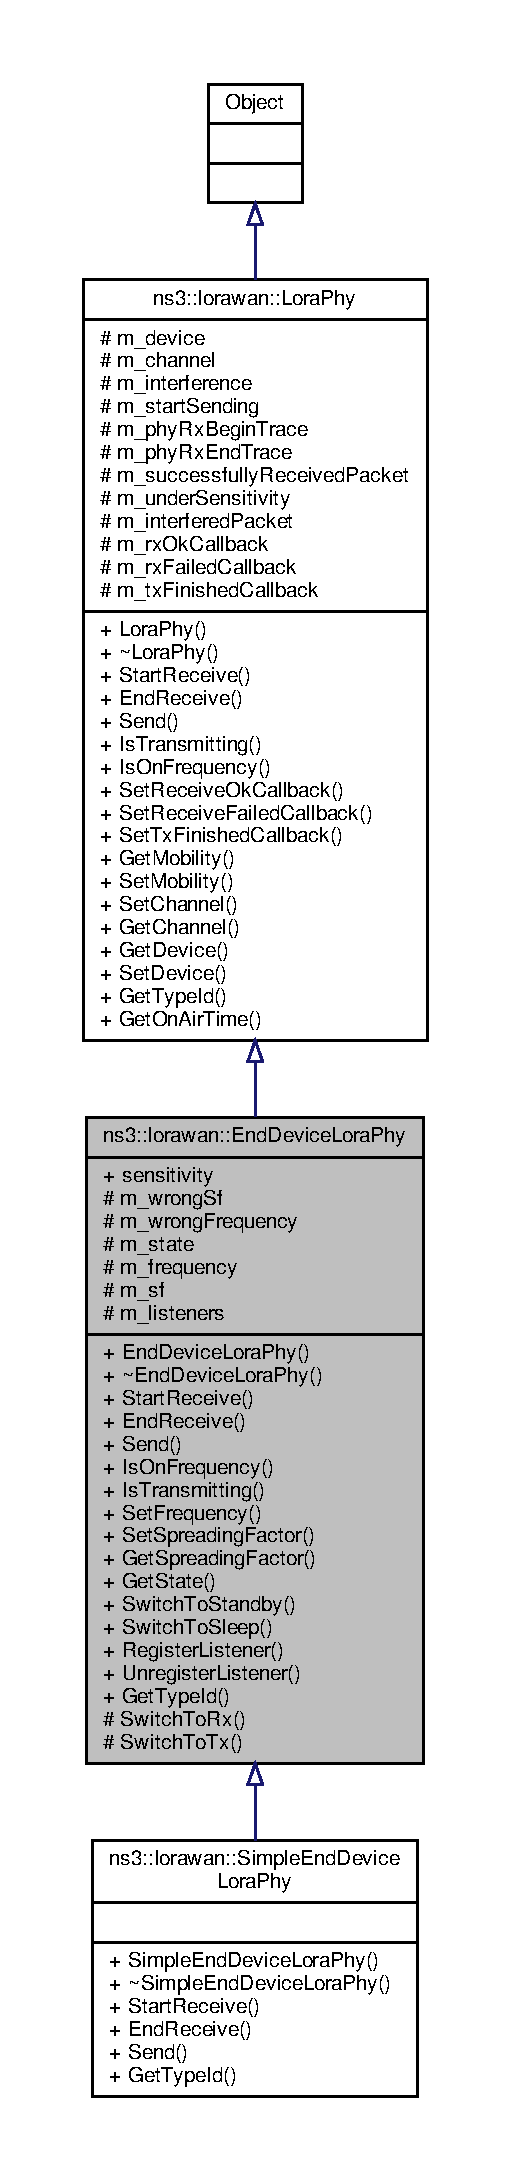
\includegraphics[height=550pt]{classns3_1_1lorawan_1_1EndDeviceLoraPhy__inherit__graph}
\end{center}
\end{figure}


Collaboration diagram for ns3\+:\+:lorawan\+:\+:End\+Device\+Lora\+Phy\+:
\nopagebreak
\begin{figure}[H]
\begin{center}
\leavevmode
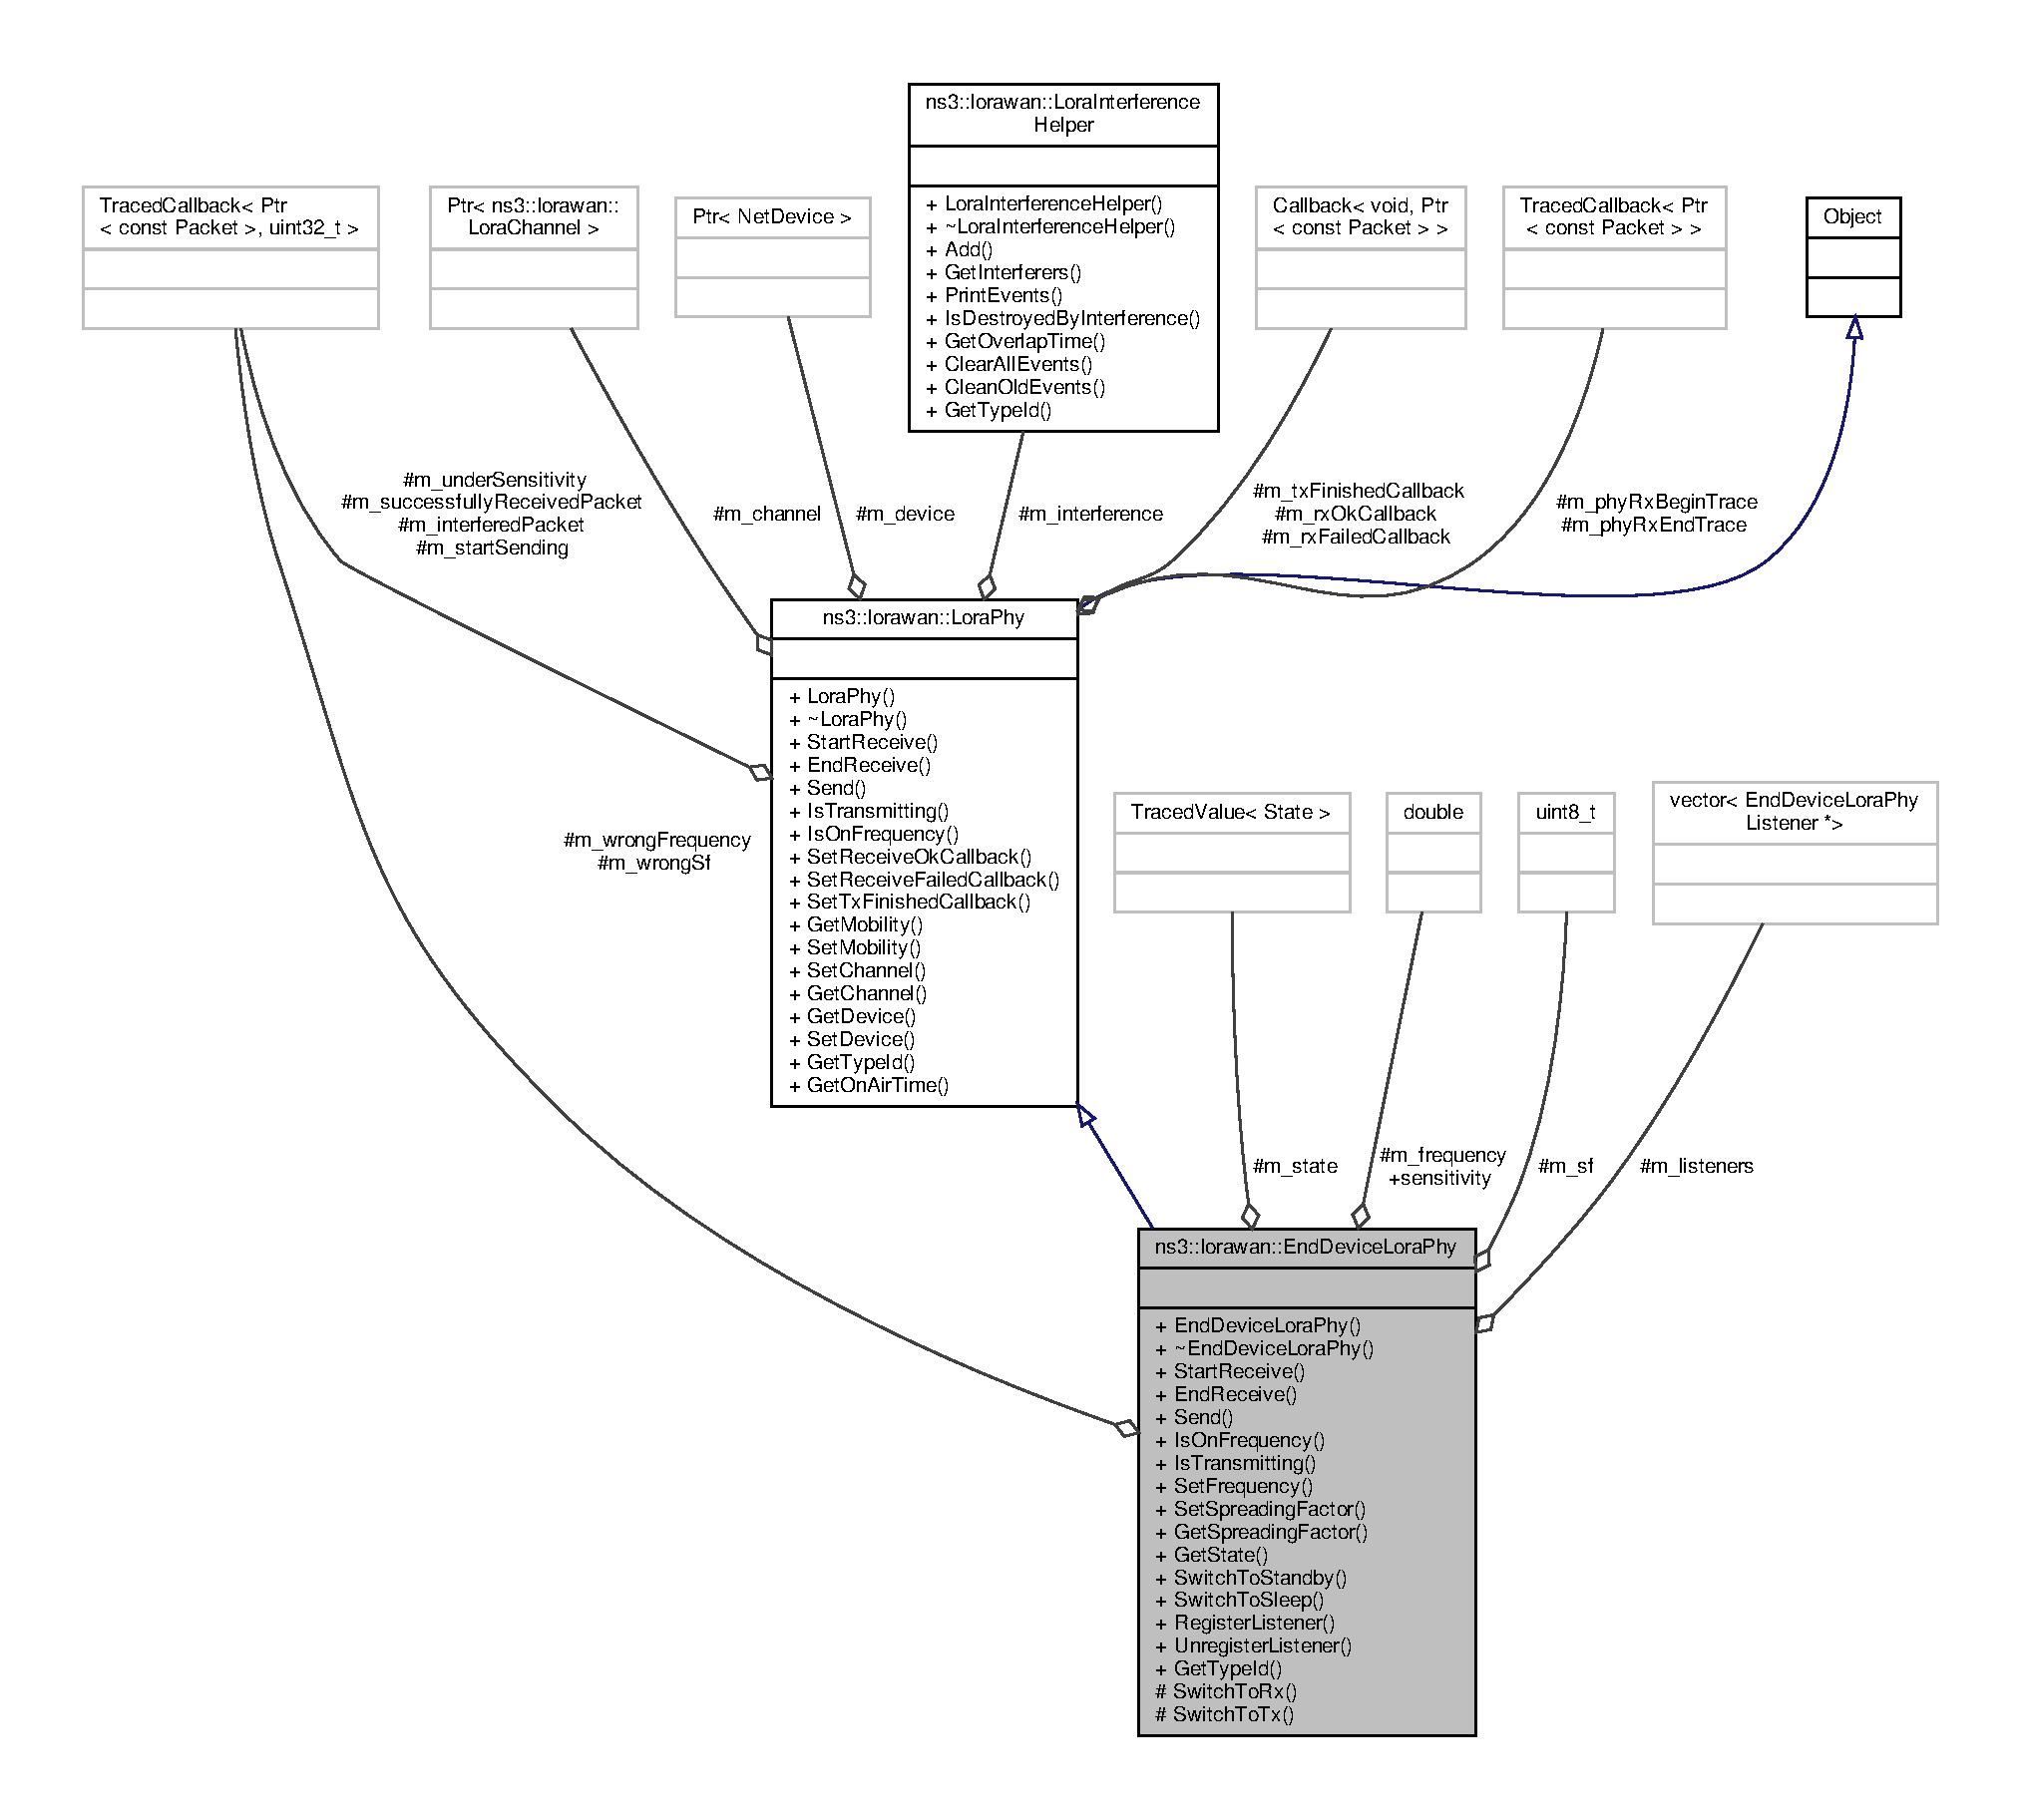
\includegraphics[width=350pt]{classns3_1_1lorawan_1_1EndDeviceLoraPhy__coll__graph}
\end{center}
\end{figure}
\subsection*{Public Types}
\begin{DoxyCompactItemize}
\item 
enum \hyperlink{classns3_1_1lorawan_1_1EndDeviceLoraPhy_adc84e4ce7796e19f19f077df9592af15}{State} \{ \hyperlink{classns3_1_1lorawan_1_1EndDeviceLoraPhy_adc84e4ce7796e19f19f077df9592af15a91cae5560efbfdfd6fa3e67de3a36aba}{S\+L\+E\+EP}, 
\hyperlink{classns3_1_1lorawan_1_1EndDeviceLoraPhy_adc84e4ce7796e19f19f077df9592af15ab546b76625ba0fd4ef3ea6cba6094786}{S\+T\+A\+N\+D\+BY}, 
\hyperlink{classns3_1_1lorawan_1_1EndDeviceLoraPhy_adc84e4ce7796e19f19f077df9592af15a35909838f2f9bf50690fefcd45628415}{TX}, 
\hyperlink{classns3_1_1lorawan_1_1EndDeviceLoraPhy_adc84e4ce7796e19f19f077df9592af15a25a7f183ed9b12f183b7fc6eb553cb5c}{RX}
 \}
\end{DoxyCompactItemize}
\subsection*{Public Member Functions}
\begin{DoxyCompactItemize}
\item 
virtual void \hyperlink{classns3_1_1lorawan_1_1EndDeviceLoraPhy_a93fbde8325d792a8fc287201482f89cb}{Start\+Receive} (Ptr$<$ Packet $>$ packet, double rx\+Power\+Dbm, uint8\+\_\+t sf, Time duration, double frequency\+M\+Hz)=0
\item 
virtual void \hyperlink{classns3_1_1lorawan_1_1EndDeviceLoraPhy_af5618e5c03f0010244fcde7922d9899f}{End\+Receive} (Ptr$<$ Packet $>$ packet, Ptr$<$ \hyperlink{classns3_1_1lorawan_1_1LoraInterferenceHelper_1_1Event}{Lora\+Interference\+Helper\+::\+Event} $>$ event)=0
\item 
virtual void \hyperlink{classns3_1_1lorawan_1_1EndDeviceLoraPhy_a47136bcb9a933e69dbf0872fbd667610}{Send} (Ptr$<$ Packet $>$ packet, \hyperlink{structns3_1_1lorawan_1_1LoraTxParameters}{Lora\+Tx\+Parameters} tx\+Params, double frequency\+M\+Hz, double tx\+Power\+Dbm)=0
\item 
virtual bool \hyperlink{classns3_1_1lorawan_1_1EndDeviceLoraPhy_a70a83e7dde5b2ae33f6f47dbbf4ad0cd}{Is\+On\+Frequency} (double frequency\+M\+Hz)
\item 
virtual bool \hyperlink{classns3_1_1lorawan_1_1EndDeviceLoraPhy_a3925d5a27b7e1352c04a78f008071d23}{Is\+Transmitting} (void)
\item 
void \hyperlink{classns3_1_1lorawan_1_1EndDeviceLoraPhy_a269afea65f27650636abe200ac4c97b8}{Set\+Frequency} (double frequency\+M\+Hz)
\item 
void \hyperlink{classns3_1_1lorawan_1_1EndDeviceLoraPhy_abc5dd987f66030a3fee58bf03de45d99}{Set\+Spreading\+Factor} (uint8\+\_\+t sf)
\item 
uint8\+\_\+t \hyperlink{classns3_1_1lorawan_1_1EndDeviceLoraPhy_ac950e8d56611b64152d206a273957f6c}{Get\+Spreading\+Factor} (void)
\item 
\hyperlink{classns3_1_1lorawan_1_1EndDeviceLoraPhy_adc84e4ce7796e19f19f077df9592af15}{End\+Device\+Lora\+Phy\+::\+State} \hyperlink{classns3_1_1lorawan_1_1EndDeviceLoraPhy_ad7cb24138a7e9769aacb97aa2472feea}{Get\+State} (void)
\item 
void \hyperlink{classns3_1_1lorawan_1_1EndDeviceLoraPhy_a698d99b5ff4a82be7ecafbd6514db156}{Switch\+To\+Standby} (void)
\item 
void \hyperlink{classns3_1_1lorawan_1_1EndDeviceLoraPhy_aa439a56b019133278eb99751fd2287f6}{Switch\+To\+Sleep} (void)
\item 
void \hyperlink{classns3_1_1lorawan_1_1EndDeviceLoraPhy_a7e7c08dc5d7926c5210e121c3dd2bfe9}{Register\+Listener} (\hyperlink{classns3_1_1lorawan_1_1EndDeviceLoraPhyListener}{End\+Device\+Lora\+Phy\+Listener} $\ast$listener)
\item 
void \hyperlink{classns3_1_1lorawan_1_1EndDeviceLoraPhy_ad1291d05e67b2a00e792f171e7621f75}{Unregister\+Listener} (\hyperlink{classns3_1_1lorawan_1_1EndDeviceLoraPhyListener}{End\+Device\+Lora\+Phy\+Listener} $\ast$listener)
\end{DoxyCompactItemize}
\subsection*{Static Public Member Functions}
\begin{DoxyCompactItemize}
\item 
\mbox{\Hypertarget{classns3_1_1lorawan_1_1EndDeviceLoraPhy_ac6c88d25b7e1e8bdd93afecd15224acb}\label{classns3_1_1lorawan_1_1EndDeviceLoraPhy_ac6c88d25b7e1e8bdd93afecd15224acb}} 
static Type\+Id {\bfseries Get\+Type\+Id} (void)
\end{DoxyCompactItemize}
\subsection*{Static Public Attributes}
\begin{DoxyCompactItemize}
\item 
static const double \hyperlink{classns3_1_1lorawan_1_1EndDeviceLoraPhy_a5fdf969286bc2cd6b357daf10122c759}{sensitivity} \mbox{[}6\mbox{]}
\begin{DoxyCompactList}\small\item\em The sensitivity vector of this device to different S\+Fs. \end{DoxyCompactList}\end{DoxyCompactItemize}
\subsection*{Protected Types}
\begin{DoxyCompactItemize}
\item 
typedef std\+::vector$<$ \hyperlink{classns3_1_1lorawan_1_1EndDeviceLoraPhyListener}{End\+Device\+Lora\+Phy\+Listener} $\ast$ $>$ \hyperlink{classns3_1_1lorawan_1_1EndDeviceLoraPhy_a2d6703f5ff4138f1a45afd26ec6223d9}{Listeners}
\item 
typedef std\+::vector$<$ \hyperlink{classns3_1_1lorawan_1_1EndDeviceLoraPhyListener}{End\+Device\+Lora\+Phy\+Listener} $\ast$ $>$\+::iterator \hyperlink{classns3_1_1lorawan_1_1EndDeviceLoraPhy_add44ac8b9f5035a0171aee9bfa271a9c}{ListenersI}
\end{DoxyCompactItemize}
\subsection*{Protected Member Functions}
\begin{DoxyCompactItemize}
\item 
void \hyperlink{classns3_1_1lorawan_1_1EndDeviceLoraPhy_a8de5dd4978c9ab0525e25991069471cf}{Switch\+To\+Rx} ()
\item 
void \hyperlink{classns3_1_1lorawan_1_1EndDeviceLoraPhy_ac73f67fb873aa6d8f1ee6c2610e6c4a8}{Switch\+To\+Tx} (double tx\+Power\+Dbm)
\end{DoxyCompactItemize}
\subsection*{Protected Attributes}
\begin{DoxyCompactItemize}
\item 
Traced\+Callback$<$ Ptr$<$ const Packet $>$, uint32\+\_\+t $>$ \hyperlink{classns3_1_1lorawan_1_1EndDeviceLoraPhy_ac3e0c1c101ab697a724622598ae208fa}{m\+\_\+wrong\+Sf}
\item 
Traced\+Callback$<$ Ptr$<$ const Packet $>$, uint32\+\_\+t $>$ \hyperlink{classns3_1_1lorawan_1_1EndDeviceLoraPhy_af8a4589c87ef5198d5a940d081959d62}{m\+\_\+wrong\+Frequency}
\item 
\mbox{\Hypertarget{classns3_1_1lorawan_1_1EndDeviceLoraPhy_ac16db644f498ae360fe7f50b5344a33c}\label{classns3_1_1lorawan_1_1EndDeviceLoraPhy_ac16db644f498ae360fe7f50b5344a33c}} 
Traced\+Value$<$ \hyperlink{classns3_1_1lorawan_1_1EndDeviceLoraPhy_adc84e4ce7796e19f19f077df9592af15}{State} $>$ \hyperlink{classns3_1_1lorawan_1_1EndDeviceLoraPhy_ac16db644f498ae360fe7f50b5344a33c}{m\+\_\+state}
\begin{DoxyCompactList}\small\item\em The state this P\+HY is currently in. \end{DoxyCompactList}\item 
\mbox{\Hypertarget{classns3_1_1lorawan_1_1EndDeviceLoraPhy_aeec9a9ac928a32278a8006d7e7dc2a0f}\label{classns3_1_1lorawan_1_1EndDeviceLoraPhy_aeec9a9ac928a32278a8006d7e7dc2a0f}} 
double \hyperlink{classns3_1_1lorawan_1_1EndDeviceLoraPhy_aeec9a9ac928a32278a8006d7e7dc2a0f}{m\+\_\+frequency}
\begin{DoxyCompactList}\small\item\em The frequency this device is listening on. \end{DoxyCompactList}\item 
\mbox{\Hypertarget{classns3_1_1lorawan_1_1EndDeviceLoraPhy_a83f682dc75f0c356d2cc7b57dd0fd991}\label{classns3_1_1lorawan_1_1EndDeviceLoraPhy_a83f682dc75f0c356d2cc7b57dd0fd991}} 
uint8\+\_\+t \hyperlink{classns3_1_1lorawan_1_1EndDeviceLoraPhy_a83f682dc75f0c356d2cc7b57dd0fd991}{m\+\_\+sf}
\begin{DoxyCompactList}\small\item\em The Spreading Factor this device is listening for. \end{DoxyCompactList}\item 
\mbox{\Hypertarget{classns3_1_1lorawan_1_1EndDeviceLoraPhy_a7953385bd2f8b872aeddf9d7dd8d47d4}\label{classns3_1_1lorawan_1_1EndDeviceLoraPhy_a7953385bd2f8b872aeddf9d7dd8d47d4}} 
\hyperlink{classns3_1_1lorawan_1_1EndDeviceLoraPhy_a2d6703f5ff4138f1a45afd26ec6223d9}{Listeners} \hyperlink{classns3_1_1lorawan_1_1EndDeviceLoraPhy_a7953385bd2f8b872aeddf9d7dd8d47d4}{m\+\_\+listeners}
\begin{DoxyCompactList}\small\item\em P\+HY listeners. \end{DoxyCompactList}\end{DoxyCompactItemize}


\subsection{Detailed Description}
Class representing a Lo\+Ra transceiver.

This class inherits some functionality by \hyperlink{classns3_1_1lorawan_1_1LoraPhy}{Lora\+Phy}, like the Get\+On\+Air\+Time function, and extends it to represent the behavior of a Lo\+Ra chip, like the S\+X1272.

Additional behaviors featured in this class include a State member variable that expresses the current state of the device (S\+L\+E\+EP, TX, RX or S\+T\+A\+N\+D\+BY), and a frequency and Spreading Factor this device is listening to when in S\+T\+A\+N\+D\+BY mode. After transmission and reception, the device returns automatically to S\+T\+A\+N\+D\+BY mode. The decision of when to go into S\+L\+E\+EP mode is delegateed to an upper layer, which can modify the state of the device through the public Switch\+To\+Sleep and Switch\+To\+Standby methods. In S\+L\+E\+EP mode, the device cannot lock on a packet and start reception.

Peculiarities about the error model and about how errors are handled are supposed to be handled by classes extending this one, like \hyperlink{classns3_1_1lorawan_1_1SimpleEndDeviceLoraPhy}{Simple\+End\+Device\+Lora\+Phy} or Spectrum\+End\+Device\+Lora\+Phy. These classes need to 

\subsection{Member Typedef Documentation}
\mbox{\Hypertarget{classns3_1_1lorawan_1_1EndDeviceLoraPhy_a2d6703f5ff4138f1a45afd26ec6223d9}\label{classns3_1_1lorawan_1_1EndDeviceLoraPhy_a2d6703f5ff4138f1a45afd26ec6223d9}} 
\index{ns3\+::lorawan\+::\+End\+Device\+Lora\+Phy@{ns3\+::lorawan\+::\+End\+Device\+Lora\+Phy}!Listeners@{Listeners}}
\index{Listeners@{Listeners}!ns3\+::lorawan\+::\+End\+Device\+Lora\+Phy@{ns3\+::lorawan\+::\+End\+Device\+Lora\+Phy}}
\subsubsection{\texorpdfstring{Listeners}{Listeners}}
{\footnotesize\ttfamily typedef std\+::vector$<$\hyperlink{classns3_1_1lorawan_1_1EndDeviceLoraPhyListener}{End\+Device\+Lora\+Phy\+Listener} $\ast$$>$ \hyperlink{classns3_1_1lorawan_1_1EndDeviceLoraPhy_a2d6703f5ff4138f1a45afd26ec6223d9}{ns3\+::lorawan\+::\+End\+Device\+Lora\+Phy\+::\+Listeners}\hspace{0.3cm}{\ttfamily [protected]}}

typedef for a list of \hyperlink{classns3_1_1lorawan_1_1EndDeviceLoraPhyListener}{End\+Device\+Lora\+Phy\+Listener} \mbox{\Hypertarget{classns3_1_1lorawan_1_1EndDeviceLoraPhy_add44ac8b9f5035a0171aee9bfa271a9c}\label{classns3_1_1lorawan_1_1EndDeviceLoraPhy_add44ac8b9f5035a0171aee9bfa271a9c}} 
\index{ns3\+::lorawan\+::\+End\+Device\+Lora\+Phy@{ns3\+::lorawan\+::\+End\+Device\+Lora\+Phy}!ListenersI@{ListenersI}}
\index{ListenersI@{ListenersI}!ns3\+::lorawan\+::\+End\+Device\+Lora\+Phy@{ns3\+::lorawan\+::\+End\+Device\+Lora\+Phy}}
\subsubsection{\texorpdfstring{ListenersI}{ListenersI}}
{\footnotesize\ttfamily typedef std\+::vector$<$\hyperlink{classns3_1_1lorawan_1_1EndDeviceLoraPhyListener}{End\+Device\+Lora\+Phy\+Listener} $\ast$$>$\+::iterator \hyperlink{classns3_1_1lorawan_1_1EndDeviceLoraPhy_add44ac8b9f5035a0171aee9bfa271a9c}{ns3\+::lorawan\+::\+End\+Device\+Lora\+Phy\+::\+ListenersI}\hspace{0.3cm}{\ttfamily [protected]}}

typedef for a list of \hyperlink{classns3_1_1lorawan_1_1EndDeviceLoraPhyListener}{End\+Device\+Lora\+Phy\+Listener} iterator 

\subsection{Member Enumeration Documentation}
\mbox{\Hypertarget{classns3_1_1lorawan_1_1EndDeviceLoraPhy_adc84e4ce7796e19f19f077df9592af15}\label{classns3_1_1lorawan_1_1EndDeviceLoraPhy_adc84e4ce7796e19f19f077df9592af15}} 
\index{ns3\+::lorawan\+::\+End\+Device\+Lora\+Phy@{ns3\+::lorawan\+::\+End\+Device\+Lora\+Phy}!State@{State}}
\index{State@{State}!ns3\+::lorawan\+::\+End\+Device\+Lora\+Phy@{ns3\+::lorawan\+::\+End\+Device\+Lora\+Phy}}
\subsubsection{\texorpdfstring{State}{State}}
{\footnotesize\ttfamily enum \hyperlink{classns3_1_1lorawan_1_1EndDeviceLoraPhy_adc84e4ce7796e19f19f077df9592af15}{ns3\+::lorawan\+::\+End\+Device\+Lora\+Phy\+::\+State}}

An enumeration of the possible states of an \hyperlink{classns3_1_1lorawan_1_1EndDeviceLoraPhy}{End\+Device\+Lora\+Phy}. It makes sense to define a state for End Devices since there\textquotesingle{}s only one demodulator which can either send, receive, stay idle or go in a deep sleep state. \begin{DoxyEnumFields}{Enumerator}
\raisebox{\heightof{T}}[0pt][0pt]{\index{S\+L\+E\+EP@{S\+L\+E\+EP}!ns3\+::lorawan\+::\+End\+Device\+Lora\+Phy@{ns3\+::lorawan\+::\+End\+Device\+Lora\+Phy}}\index{ns3\+::lorawan\+::\+End\+Device\+Lora\+Phy@{ns3\+::lorawan\+::\+End\+Device\+Lora\+Phy}!S\+L\+E\+EP@{S\+L\+E\+EP}}}\mbox{\Hypertarget{classns3_1_1lorawan_1_1EndDeviceLoraPhy_adc84e4ce7796e19f19f077df9592af15a91cae5560efbfdfd6fa3e67de3a36aba}\label{classns3_1_1lorawan_1_1EndDeviceLoraPhy_adc84e4ce7796e19f19f077df9592af15a91cae5560efbfdfd6fa3e67de3a36aba}} 
S\+L\+E\+EP&The P\+HY layer is sleeping. During sleep, the device is not listening for incoming messages. \\
\hline

\raisebox{\heightof{T}}[0pt][0pt]{\index{S\+T\+A\+N\+D\+BY@{S\+T\+A\+N\+D\+BY}!ns3\+::lorawan\+::\+End\+Device\+Lora\+Phy@{ns3\+::lorawan\+::\+End\+Device\+Lora\+Phy}}\index{ns3\+::lorawan\+::\+End\+Device\+Lora\+Phy@{ns3\+::lorawan\+::\+End\+Device\+Lora\+Phy}!S\+T\+A\+N\+D\+BY@{S\+T\+A\+N\+D\+BY}}}\mbox{\Hypertarget{classns3_1_1lorawan_1_1EndDeviceLoraPhy_adc84e4ce7796e19f19f077df9592af15ab546b76625ba0fd4ef3ea6cba6094786}\label{classns3_1_1lorawan_1_1EndDeviceLoraPhy_adc84e4ce7796e19f19f077df9592af15ab546b76625ba0fd4ef3ea6cba6094786}} 
S\+T\+A\+N\+D\+BY&The P\+HY layer is in S\+T\+A\+N\+D\+BY. When the P\+HY is in this state, it\textquotesingle{}s listening to the channel, and it\textquotesingle{}s also ready to transmit data passed to it by the M\+AC layer. \\
\hline

\raisebox{\heightof{T}}[0pt][0pt]{\index{TX@{TX}!ns3\+::lorawan\+::\+End\+Device\+Lora\+Phy@{ns3\+::lorawan\+::\+End\+Device\+Lora\+Phy}}\index{ns3\+::lorawan\+::\+End\+Device\+Lora\+Phy@{ns3\+::lorawan\+::\+End\+Device\+Lora\+Phy}!TX@{TX}}}\mbox{\Hypertarget{classns3_1_1lorawan_1_1EndDeviceLoraPhy_adc84e4ce7796e19f19f077df9592af15a35909838f2f9bf50690fefcd45628415}\label{classns3_1_1lorawan_1_1EndDeviceLoraPhy_adc84e4ce7796e19f19f077df9592af15a35909838f2f9bf50690fefcd45628415}} 
TX&The P\+HY layer is sending a packet. During transmission, the device cannot receive any packet or send any additional packet. \\
\hline

\raisebox{\heightof{T}}[0pt][0pt]{\index{RX@{RX}!ns3\+::lorawan\+::\+End\+Device\+Lora\+Phy@{ns3\+::lorawan\+::\+End\+Device\+Lora\+Phy}}\index{ns3\+::lorawan\+::\+End\+Device\+Lora\+Phy@{ns3\+::lorawan\+::\+End\+Device\+Lora\+Phy}!RX@{RX}}}\mbox{\Hypertarget{classns3_1_1lorawan_1_1EndDeviceLoraPhy_adc84e4ce7796e19f19f077df9592af15a25a7f183ed9b12f183b7fc6eb553cb5c}\label{classns3_1_1lorawan_1_1EndDeviceLoraPhy_adc84e4ce7796e19f19f077df9592af15a25a7f183ed9b12f183b7fc6eb553cb5c}} 
RX&The P\+HY layer is receiving a packet. While the device is locked on an incoming packet, transmission is not possible. \\
\hline

\end{DoxyEnumFields}


\subsection{Member Function Documentation}
\mbox{\Hypertarget{classns3_1_1lorawan_1_1EndDeviceLoraPhy_af5618e5c03f0010244fcde7922d9899f}\label{classns3_1_1lorawan_1_1EndDeviceLoraPhy_af5618e5c03f0010244fcde7922d9899f}} 
\index{ns3\+::lorawan\+::\+End\+Device\+Lora\+Phy@{ns3\+::lorawan\+::\+End\+Device\+Lora\+Phy}!End\+Receive@{End\+Receive}}
\index{End\+Receive@{End\+Receive}!ns3\+::lorawan\+::\+End\+Device\+Lora\+Phy@{ns3\+::lorawan\+::\+End\+Device\+Lora\+Phy}}
\subsubsection{\texorpdfstring{End\+Receive()}{EndReceive()}}
{\footnotesize\ttfamily virtual void ns3\+::lorawan\+::\+End\+Device\+Lora\+Phy\+::\+End\+Receive (\begin{DoxyParamCaption}\item[{Ptr$<$ Packet $>$}]{packet,  }\item[{Ptr$<$ \hyperlink{classns3_1_1lorawan_1_1LoraInterferenceHelper_1_1Event}{Lora\+Interference\+Helper\+::\+Event} $>$}]{event }\end{DoxyParamCaption})\hspace{0.3cm}{\ttfamily [pure virtual]}}

Finish reception of a packet.

This method is scheduled by Start\+Receive, based on the packet duration. By passing a \hyperlink{classns3_1_1lorawan_1_1LoraInterferenceHelper}{Lora\+Interference\+Helper} Event to this method, the class will be able to identify the packet that is being received among all those that were registered as interference by Start\+Receive.


\begin{DoxyParams}{Parameters}
{\em packet} & The received packet. \\
\hline
{\em event} & The event that is tied to this packet in the \hyperlink{classns3_1_1lorawan_1_1LoraInterferenceHelper}{Lora\+Interference\+Helper}. \\
\hline
\end{DoxyParams}


Implements \hyperlink{classns3_1_1lorawan_1_1LoraPhy_a719f749890c247abc3fda290d384c37f}{ns3\+::lorawan\+::\+Lora\+Phy}.



Implemented in \hyperlink{classns3_1_1lorawan_1_1SimpleEndDeviceLoraPhy_a03a9d0ffdd5f89991a61aa54e5a1e7ba}{ns3\+::lorawan\+::\+Simple\+End\+Device\+Lora\+Phy}.

\mbox{\Hypertarget{classns3_1_1lorawan_1_1EndDeviceLoraPhy_ac950e8d56611b64152d206a273957f6c}\label{classns3_1_1lorawan_1_1EndDeviceLoraPhy_ac950e8d56611b64152d206a273957f6c}} 
\index{ns3\+::lorawan\+::\+End\+Device\+Lora\+Phy@{ns3\+::lorawan\+::\+End\+Device\+Lora\+Phy}!Get\+Spreading\+Factor@{Get\+Spreading\+Factor}}
\index{Get\+Spreading\+Factor@{Get\+Spreading\+Factor}!ns3\+::lorawan\+::\+End\+Device\+Lora\+Phy@{ns3\+::lorawan\+::\+End\+Device\+Lora\+Phy}}
\subsubsection{\texorpdfstring{Get\+Spreading\+Factor()}{GetSpreadingFactor()}}
{\footnotesize\ttfamily uint8\+\_\+t ns3\+::lorawan\+::\+End\+Device\+Lora\+Phy\+::\+Get\+Spreading\+Factor (\begin{DoxyParamCaption}\item[{void}]{ }\end{DoxyParamCaption})}

Get the Spreading Factor this End\+Device is listening for.

\begin{DoxyReturn}{Returns}
The Spreading Factor we are listening for. 
\end{DoxyReturn}
\mbox{\Hypertarget{classns3_1_1lorawan_1_1EndDeviceLoraPhy_ad7cb24138a7e9769aacb97aa2472feea}\label{classns3_1_1lorawan_1_1EndDeviceLoraPhy_ad7cb24138a7e9769aacb97aa2472feea}} 
\index{ns3\+::lorawan\+::\+End\+Device\+Lora\+Phy@{ns3\+::lorawan\+::\+End\+Device\+Lora\+Phy}!Get\+State@{Get\+State}}
\index{Get\+State@{Get\+State}!ns3\+::lorawan\+::\+End\+Device\+Lora\+Phy@{ns3\+::lorawan\+::\+End\+Device\+Lora\+Phy}}
\subsubsection{\texorpdfstring{Get\+State()}{GetState()}}
{\footnotesize\ttfamily \hyperlink{classns3_1_1lorawan_1_1EndDeviceLoraPhy_adc84e4ce7796e19f19f077df9592af15}{End\+Device\+Lora\+Phy\+::\+State} ns3\+::lorawan\+::\+End\+Device\+Lora\+Phy\+::\+Get\+State (\begin{DoxyParamCaption}\item[{void}]{ }\end{DoxyParamCaption})}

Return the state this End Device is currently in.

\begin{DoxyReturn}{Returns}
The state this \hyperlink{classns3_1_1lorawan_1_1EndDeviceLoraPhy}{End\+Device\+Lora\+Phy} is currently in. 
\end{DoxyReturn}
\mbox{\Hypertarget{classns3_1_1lorawan_1_1EndDeviceLoraPhy_a70a83e7dde5b2ae33f6f47dbbf4ad0cd}\label{classns3_1_1lorawan_1_1EndDeviceLoraPhy_a70a83e7dde5b2ae33f6f47dbbf4ad0cd}} 
\index{ns3\+::lorawan\+::\+End\+Device\+Lora\+Phy@{ns3\+::lorawan\+::\+End\+Device\+Lora\+Phy}!Is\+On\+Frequency@{Is\+On\+Frequency}}
\index{Is\+On\+Frequency@{Is\+On\+Frequency}!ns3\+::lorawan\+::\+End\+Device\+Lora\+Phy@{ns3\+::lorawan\+::\+End\+Device\+Lora\+Phy}}
\subsubsection{\texorpdfstring{Is\+On\+Frequency()}{IsOnFrequency()}}
{\footnotesize\ttfamily bool ns3\+::lorawan\+::\+End\+Device\+Lora\+Phy\+::\+Is\+On\+Frequency (\begin{DoxyParamCaption}\item[{double}]{frequency }\end{DoxyParamCaption})\hspace{0.3cm}{\ttfamily [virtual]}}

Whether this device is listening on the specified frequency or not.


\begin{DoxyParams}{Parameters}
{\em frequency} & The frequency to query. \\
\hline
\end{DoxyParams}
\begin{DoxyReturn}{Returns}
true if the device is listening on that frequency, false otherwise. 
\end{DoxyReturn}


Implements \hyperlink{classns3_1_1lorawan_1_1LoraPhy_a554597e30a17b099e8a7f68242cb16a7}{ns3\+::lorawan\+::\+Lora\+Phy}.

\mbox{\Hypertarget{classns3_1_1lorawan_1_1EndDeviceLoraPhy_a3925d5a27b7e1352c04a78f008071d23}\label{classns3_1_1lorawan_1_1EndDeviceLoraPhy_a3925d5a27b7e1352c04a78f008071d23}} 
\index{ns3\+::lorawan\+::\+End\+Device\+Lora\+Phy@{ns3\+::lorawan\+::\+End\+Device\+Lora\+Phy}!Is\+Transmitting@{Is\+Transmitting}}
\index{Is\+Transmitting@{Is\+Transmitting}!ns3\+::lorawan\+::\+End\+Device\+Lora\+Phy@{ns3\+::lorawan\+::\+End\+Device\+Lora\+Phy}}
\subsubsection{\texorpdfstring{Is\+Transmitting()}{IsTransmitting()}}
{\footnotesize\ttfamily bool ns3\+::lorawan\+::\+End\+Device\+Lora\+Phy\+::\+Is\+Transmitting (\begin{DoxyParamCaption}\item[{void}]{ }\end{DoxyParamCaption})\hspace{0.3cm}{\ttfamily [virtual]}}

Whether this device is transmitting or not.

\begin{DoxyReturn}{Returns}
true if the device is currently transmitting a packet, false otherwise. 
\end{DoxyReturn}


Implements \hyperlink{classns3_1_1lorawan_1_1LoraPhy_a5280764d934ba5ff8d305b0bc6b600ce}{ns3\+::lorawan\+::\+Lora\+Phy}.

\mbox{\Hypertarget{classns3_1_1lorawan_1_1EndDeviceLoraPhy_a7e7c08dc5d7926c5210e121c3dd2bfe9}\label{classns3_1_1lorawan_1_1EndDeviceLoraPhy_a7e7c08dc5d7926c5210e121c3dd2bfe9}} 
\index{ns3\+::lorawan\+::\+End\+Device\+Lora\+Phy@{ns3\+::lorawan\+::\+End\+Device\+Lora\+Phy}!Register\+Listener@{Register\+Listener}}
\index{Register\+Listener@{Register\+Listener}!ns3\+::lorawan\+::\+End\+Device\+Lora\+Phy@{ns3\+::lorawan\+::\+End\+Device\+Lora\+Phy}}
\subsubsection{\texorpdfstring{Register\+Listener()}{RegisterListener()}}
{\footnotesize\ttfamily void ns3\+::lorawan\+::\+End\+Device\+Lora\+Phy\+::\+Register\+Listener (\begin{DoxyParamCaption}\item[{\hyperlink{classns3_1_1lorawan_1_1EndDeviceLoraPhyListener}{End\+Device\+Lora\+Phy\+Listener} $\ast$}]{listener }\end{DoxyParamCaption})}

Add the input listener to the list of objects to be notified of P\+H\+Y-\/level events.


\begin{DoxyParams}{Parameters}
{\em listener} & the new listener \\
\hline
\end{DoxyParams}
\mbox{\Hypertarget{classns3_1_1lorawan_1_1EndDeviceLoraPhy_a47136bcb9a933e69dbf0872fbd667610}\label{classns3_1_1lorawan_1_1EndDeviceLoraPhy_a47136bcb9a933e69dbf0872fbd667610}} 
\index{ns3\+::lorawan\+::\+End\+Device\+Lora\+Phy@{ns3\+::lorawan\+::\+End\+Device\+Lora\+Phy}!Send@{Send}}
\index{Send@{Send}!ns3\+::lorawan\+::\+End\+Device\+Lora\+Phy@{ns3\+::lorawan\+::\+End\+Device\+Lora\+Phy}}
\subsubsection{\texorpdfstring{Send()}{Send()}}
{\footnotesize\ttfamily virtual void ns3\+::lorawan\+::\+End\+Device\+Lora\+Phy\+::\+Send (\begin{DoxyParamCaption}\item[{Ptr$<$ Packet $>$}]{packet,  }\item[{\hyperlink{structns3_1_1lorawan_1_1LoraTxParameters}{Lora\+Tx\+Parameters}}]{tx\+Params,  }\item[{double}]{frequency\+M\+Hz,  }\item[{double}]{tx\+Power\+Dbm }\end{DoxyParamCaption})\hspace{0.3cm}{\ttfamily [pure virtual]}}

Instruct the P\+HY to send a packet according to some parameters.


\begin{DoxyParams}{Parameters}
{\em packet} & The packet to send. \\
\hline
{\em tx\+Params} & The desired transmission parameters. \\
\hline
{\em frequency\+M\+Hz} & The frequency on which to transmit. \\
\hline
{\em tx\+Power\+Dbm} & The power in d\+Bm with which to transmit the packet. \\
\hline
\end{DoxyParams}


Implements \hyperlink{classns3_1_1lorawan_1_1LoraPhy_a2b940beff4a2fbfb2e603d5d9e65d863}{ns3\+::lorawan\+::\+Lora\+Phy}.



Implemented in \hyperlink{classns3_1_1lorawan_1_1SimpleEndDeviceLoraPhy_a5698d15e92de30b7f9178af3997b89e9}{ns3\+::lorawan\+::\+Simple\+End\+Device\+Lora\+Phy}.

\mbox{\Hypertarget{classns3_1_1lorawan_1_1EndDeviceLoraPhy_a269afea65f27650636abe200ac4c97b8}\label{classns3_1_1lorawan_1_1EndDeviceLoraPhy_a269afea65f27650636abe200ac4c97b8}} 
\index{ns3\+::lorawan\+::\+End\+Device\+Lora\+Phy@{ns3\+::lorawan\+::\+End\+Device\+Lora\+Phy}!Set\+Frequency@{Set\+Frequency}}
\index{Set\+Frequency@{Set\+Frequency}!ns3\+::lorawan\+::\+End\+Device\+Lora\+Phy@{ns3\+::lorawan\+::\+End\+Device\+Lora\+Phy}}
\subsubsection{\texorpdfstring{Set\+Frequency()}{SetFrequency()}}
{\footnotesize\ttfamily void ns3\+::lorawan\+::\+End\+Device\+Lora\+Phy\+::\+Set\+Frequency (\begin{DoxyParamCaption}\item[{double}]{frequency\+M\+Hz }\end{DoxyParamCaption})}

Set the frequency this End\+Device will listen on.

Should a packet be transmitted on a frequency different than that the \hyperlink{classns3_1_1lorawan_1_1EndDeviceLoraPhy}{End\+Device\+Lora\+Phy} is listening on, the packet will be discarded.


\begin{DoxyParams}{Parameters}
{\em The} & frequency \mbox{[}M\+Hz\mbox{]} to listen to. \\
\hline
\end{DoxyParams}
\mbox{\Hypertarget{classns3_1_1lorawan_1_1EndDeviceLoraPhy_abc5dd987f66030a3fee58bf03de45d99}\label{classns3_1_1lorawan_1_1EndDeviceLoraPhy_abc5dd987f66030a3fee58bf03de45d99}} 
\index{ns3\+::lorawan\+::\+End\+Device\+Lora\+Phy@{ns3\+::lorawan\+::\+End\+Device\+Lora\+Phy}!Set\+Spreading\+Factor@{Set\+Spreading\+Factor}}
\index{Set\+Spreading\+Factor@{Set\+Spreading\+Factor}!ns3\+::lorawan\+::\+End\+Device\+Lora\+Phy@{ns3\+::lorawan\+::\+End\+Device\+Lora\+Phy}}
\subsubsection{\texorpdfstring{Set\+Spreading\+Factor()}{SetSpreadingFactor()}}
{\footnotesize\ttfamily void ns3\+::lorawan\+::\+End\+Device\+Lora\+Phy\+::\+Set\+Spreading\+Factor (\begin{DoxyParamCaption}\item[{uint8\+\_\+t}]{sf }\end{DoxyParamCaption})}

Set the Spreading Factor this End\+Device will listen for.

The \hyperlink{classns3_1_1lorawan_1_1EndDeviceLoraPhy}{End\+Device\+Lora\+Phy} object will not be able to lock on transmissions that use a different SF than the one it\textquotesingle{}s listening for.


\begin{DoxyParams}{Parameters}
{\em sf} & The spreading factor to listen for. \\
\hline
\end{DoxyParams}
\mbox{\Hypertarget{classns3_1_1lorawan_1_1EndDeviceLoraPhy_a93fbde8325d792a8fc287201482f89cb}\label{classns3_1_1lorawan_1_1EndDeviceLoraPhy_a93fbde8325d792a8fc287201482f89cb}} 
\index{ns3\+::lorawan\+::\+End\+Device\+Lora\+Phy@{ns3\+::lorawan\+::\+End\+Device\+Lora\+Phy}!Start\+Receive@{Start\+Receive}}
\index{Start\+Receive@{Start\+Receive}!ns3\+::lorawan\+::\+End\+Device\+Lora\+Phy@{ns3\+::lorawan\+::\+End\+Device\+Lora\+Phy}}
\subsubsection{\texorpdfstring{Start\+Receive()}{StartReceive()}}
{\footnotesize\ttfamily virtual void ns3\+::lorawan\+::\+End\+Device\+Lora\+Phy\+::\+Start\+Receive (\begin{DoxyParamCaption}\item[{Ptr$<$ Packet $>$}]{packet,  }\item[{double}]{rx\+Power\+Dbm,  }\item[{uint8\+\_\+t}]{sf,  }\item[{Time}]{duration,  }\item[{double}]{frequency\+M\+Hz }\end{DoxyParamCaption})\hspace{0.3cm}{\ttfamily [pure virtual]}}

Start receiving a packet.

This method is typically called by \hyperlink{classns3_1_1lorawan_1_1LoraChannel}{Lora\+Channel}.


\begin{DoxyParams}{Parameters}
{\em packet} & The packet that is arriving at this P\+HY layer. \\
\hline
{\em rx\+Power\+Dbm} & The power of the arriving packet (assumed to be constant for the whole reception). \\
\hline
{\em sf} & The Spreading Factor of the arriving packet. \\
\hline
{\em duration} & The on air time of this packet. \\
\hline
{\em frequency\+M\+Hz} & The frequency this packet is being transmitted on. \\
\hline
\end{DoxyParams}


Implements \hyperlink{classns3_1_1lorawan_1_1LoraPhy_aeeccb517d12084e12e36b533db22386b}{ns3\+::lorawan\+::\+Lora\+Phy}.



Implemented in \hyperlink{classns3_1_1lorawan_1_1SimpleEndDeviceLoraPhy_ad7a421670937fa0c4ece217ae02598ad}{ns3\+::lorawan\+::\+Simple\+End\+Device\+Lora\+Phy}.

\mbox{\Hypertarget{classns3_1_1lorawan_1_1EndDeviceLoraPhy_a8de5dd4978c9ab0525e25991069471cf}\label{classns3_1_1lorawan_1_1EndDeviceLoraPhy_a8de5dd4978c9ab0525e25991069471cf}} 
\index{ns3\+::lorawan\+::\+End\+Device\+Lora\+Phy@{ns3\+::lorawan\+::\+End\+Device\+Lora\+Phy}!Switch\+To\+Rx@{Switch\+To\+Rx}}
\index{Switch\+To\+Rx@{Switch\+To\+Rx}!ns3\+::lorawan\+::\+End\+Device\+Lora\+Phy@{ns3\+::lorawan\+::\+End\+Device\+Lora\+Phy}}
\subsubsection{\texorpdfstring{Switch\+To\+Rx()}{SwitchToRx()}}
{\footnotesize\ttfamily void ns3\+::lorawan\+::\+End\+Device\+Lora\+Phy\+::\+Switch\+To\+Rx (\begin{DoxyParamCaption}\item[{void}]{ }\end{DoxyParamCaption})\hspace{0.3cm}{\ttfamily [protected]}}

Switch to the RX state \mbox{\Hypertarget{classns3_1_1lorawan_1_1EndDeviceLoraPhy_aa439a56b019133278eb99751fd2287f6}\label{classns3_1_1lorawan_1_1EndDeviceLoraPhy_aa439a56b019133278eb99751fd2287f6}} 
\index{ns3\+::lorawan\+::\+End\+Device\+Lora\+Phy@{ns3\+::lorawan\+::\+End\+Device\+Lora\+Phy}!Switch\+To\+Sleep@{Switch\+To\+Sleep}}
\index{Switch\+To\+Sleep@{Switch\+To\+Sleep}!ns3\+::lorawan\+::\+End\+Device\+Lora\+Phy@{ns3\+::lorawan\+::\+End\+Device\+Lora\+Phy}}
\subsubsection{\texorpdfstring{Switch\+To\+Sleep()}{SwitchToSleep()}}
{\footnotesize\ttfamily void ns3\+::lorawan\+::\+End\+Device\+Lora\+Phy\+::\+Switch\+To\+Sleep (\begin{DoxyParamCaption}\item[{void}]{ }\end{DoxyParamCaption})}

Switch to the S\+L\+E\+EP state. \mbox{\Hypertarget{classns3_1_1lorawan_1_1EndDeviceLoraPhy_a698d99b5ff4a82be7ecafbd6514db156}\label{classns3_1_1lorawan_1_1EndDeviceLoraPhy_a698d99b5ff4a82be7ecafbd6514db156}} 
\index{ns3\+::lorawan\+::\+End\+Device\+Lora\+Phy@{ns3\+::lorawan\+::\+End\+Device\+Lora\+Phy}!Switch\+To\+Standby@{Switch\+To\+Standby}}
\index{Switch\+To\+Standby@{Switch\+To\+Standby}!ns3\+::lorawan\+::\+End\+Device\+Lora\+Phy@{ns3\+::lorawan\+::\+End\+Device\+Lora\+Phy}}
\subsubsection{\texorpdfstring{Switch\+To\+Standby()}{SwitchToStandby()}}
{\footnotesize\ttfamily void ns3\+::lorawan\+::\+End\+Device\+Lora\+Phy\+::\+Switch\+To\+Standby (\begin{DoxyParamCaption}\item[{void}]{ }\end{DoxyParamCaption})}

Switch to the S\+T\+A\+N\+D\+BY state. \mbox{\Hypertarget{classns3_1_1lorawan_1_1EndDeviceLoraPhy_ac73f67fb873aa6d8f1ee6c2610e6c4a8}\label{classns3_1_1lorawan_1_1EndDeviceLoraPhy_ac73f67fb873aa6d8f1ee6c2610e6c4a8}} 
\index{ns3\+::lorawan\+::\+End\+Device\+Lora\+Phy@{ns3\+::lorawan\+::\+End\+Device\+Lora\+Phy}!Switch\+To\+Tx@{Switch\+To\+Tx}}
\index{Switch\+To\+Tx@{Switch\+To\+Tx}!ns3\+::lorawan\+::\+End\+Device\+Lora\+Phy@{ns3\+::lorawan\+::\+End\+Device\+Lora\+Phy}}
\subsubsection{\texorpdfstring{Switch\+To\+Tx()}{SwitchToTx()}}
{\footnotesize\ttfamily void ns3\+::lorawan\+::\+End\+Device\+Lora\+Phy\+::\+Switch\+To\+Tx (\begin{DoxyParamCaption}\item[{double}]{tx\+Power\+Dbm }\end{DoxyParamCaption})\hspace{0.3cm}{\ttfamily [protected]}}

Switch to the TX state \mbox{\Hypertarget{classns3_1_1lorawan_1_1EndDeviceLoraPhy_ad1291d05e67b2a00e792f171e7621f75}\label{classns3_1_1lorawan_1_1EndDeviceLoraPhy_ad1291d05e67b2a00e792f171e7621f75}} 
\index{ns3\+::lorawan\+::\+End\+Device\+Lora\+Phy@{ns3\+::lorawan\+::\+End\+Device\+Lora\+Phy}!Unregister\+Listener@{Unregister\+Listener}}
\index{Unregister\+Listener@{Unregister\+Listener}!ns3\+::lorawan\+::\+End\+Device\+Lora\+Phy@{ns3\+::lorawan\+::\+End\+Device\+Lora\+Phy}}
\subsubsection{\texorpdfstring{Unregister\+Listener()}{UnregisterListener()}}
{\footnotesize\ttfamily void ns3\+::lorawan\+::\+End\+Device\+Lora\+Phy\+::\+Unregister\+Listener (\begin{DoxyParamCaption}\item[{\hyperlink{classns3_1_1lorawan_1_1EndDeviceLoraPhyListener}{End\+Device\+Lora\+Phy\+Listener} $\ast$}]{listener }\end{DoxyParamCaption})}

Remove the input listener from the list of objects to be notified of P\+H\+Y-\/level events.


\begin{DoxyParams}{Parameters}
{\em listener} & the listener to be unregistered \\
\hline
\end{DoxyParams}


\subsection{Member Data Documentation}
\mbox{\Hypertarget{classns3_1_1lorawan_1_1EndDeviceLoraPhy_af8a4589c87ef5198d5a940d081959d62}\label{classns3_1_1lorawan_1_1EndDeviceLoraPhy_af8a4589c87ef5198d5a940d081959d62}} 
\index{ns3\+::lorawan\+::\+End\+Device\+Lora\+Phy@{ns3\+::lorawan\+::\+End\+Device\+Lora\+Phy}!m\+\_\+wrong\+Frequency@{m\+\_\+wrong\+Frequency}}
\index{m\+\_\+wrong\+Frequency@{m\+\_\+wrong\+Frequency}!ns3\+::lorawan\+::\+End\+Device\+Lora\+Phy@{ns3\+::lorawan\+::\+End\+Device\+Lora\+Phy}}
\subsubsection{\texorpdfstring{m\+\_\+wrong\+Frequency}{m\_wrongFrequency}}
{\footnotesize\ttfamily Traced\+Callback$<$Ptr$<$const Packet$>$, uint32\+\_\+t$>$ ns3\+::lorawan\+::\+End\+Device\+Lora\+Phy\+::m\+\_\+wrong\+Frequency\hspace{0.3cm}{\ttfamily [protected]}}

Trace source for when a packet is lost because it was transmitted on a frequency different from the one this \hyperlink{classns3_1_1lorawan_1_1EndDeviceLoraPhy}{End\+Device\+Lora\+Phy} was configured to listen on. \mbox{\Hypertarget{classns3_1_1lorawan_1_1EndDeviceLoraPhy_ac3e0c1c101ab697a724622598ae208fa}\label{classns3_1_1lorawan_1_1EndDeviceLoraPhy_ac3e0c1c101ab697a724622598ae208fa}} 
\index{ns3\+::lorawan\+::\+End\+Device\+Lora\+Phy@{ns3\+::lorawan\+::\+End\+Device\+Lora\+Phy}!m\+\_\+wrong\+Sf@{m\+\_\+wrong\+Sf}}
\index{m\+\_\+wrong\+Sf@{m\+\_\+wrong\+Sf}!ns3\+::lorawan\+::\+End\+Device\+Lora\+Phy@{ns3\+::lorawan\+::\+End\+Device\+Lora\+Phy}}
\subsubsection{\texorpdfstring{m\+\_\+wrong\+Sf}{m\_wrongSf}}
{\footnotesize\ttfamily Traced\+Callback$<$Ptr$<$const Packet$>$, uint32\+\_\+t$>$ ns3\+::lorawan\+::\+End\+Device\+Lora\+Phy\+::m\+\_\+wrong\+Sf\hspace{0.3cm}{\ttfamily [protected]}}

Trace source for when a packet is lost because it was using a SF different from the one this \hyperlink{classns3_1_1lorawan_1_1EndDeviceLoraPhy}{End\+Device\+Lora\+Phy} was configured to listen for. \mbox{\Hypertarget{classns3_1_1lorawan_1_1EndDeviceLoraPhy_a5fdf969286bc2cd6b357daf10122c759}\label{classns3_1_1lorawan_1_1EndDeviceLoraPhy_a5fdf969286bc2cd6b357daf10122c759}} 
\index{ns3\+::lorawan\+::\+End\+Device\+Lora\+Phy@{ns3\+::lorawan\+::\+End\+Device\+Lora\+Phy}!sensitivity@{sensitivity}}
\index{sensitivity@{sensitivity}!ns3\+::lorawan\+::\+End\+Device\+Lora\+Phy@{ns3\+::lorawan\+::\+End\+Device\+Lora\+Phy}}
\subsubsection{\texorpdfstring{sensitivity}{sensitivity}}
{\footnotesize\ttfamily const double ns3\+::lorawan\+::\+End\+Device\+Lora\+Phy\+::sensitivity\hspace{0.3cm}{\ttfamily [static]}}

{\bfseries Initial value\+:}
\begin{DoxyCode}
= \{-124, -127, -130,
                                                                                                 -133, -135
      , -137\}
\end{DoxyCode}


The sensitivity vector of this device to different S\+Fs. 



The documentation for this class was generated from the following files\+:\begin{DoxyCompactItemize}
\item 
end-\/device-\/lora-\/phy.\+h\item 
end-\/device-\/lora-\/phy.\+cc\end{DoxyCompactItemize}

\hypertarget{classns3_1_1lorawan_1_1EndDeviceLoraPhyListener}{}\section{ns3\+:\+:lorawan\+:\+:End\+Device\+Lora\+Phy\+Listener Class Reference}
\label{classns3_1_1lorawan_1_1EndDeviceLoraPhyListener}\index{ns3\+::lorawan\+::\+End\+Device\+Lora\+Phy\+Listener@{ns3\+::lorawan\+::\+End\+Device\+Lora\+Phy\+Listener}}


{\ttfamily \#include $<$end-\/device-\/lora-\/phy.\+h$>$}



Inheritance diagram for ns3\+:\+:lorawan\+:\+:End\+Device\+Lora\+Phy\+Listener\+:
\nopagebreak
\begin{figure}[H]
\begin{center}
\leavevmode
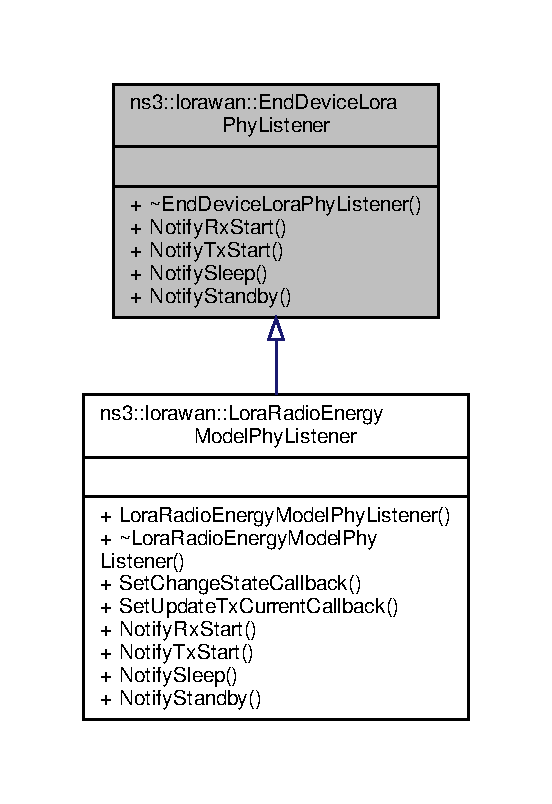
\includegraphics[width=265pt]{classns3_1_1lorawan_1_1EndDeviceLoraPhyListener__inherit__graph}
\end{center}
\end{figure}


Collaboration diagram for ns3\+:\+:lorawan\+:\+:End\+Device\+Lora\+Phy\+Listener\+:
\nopagebreak
\begin{figure}[H]
\begin{center}
\leavevmode
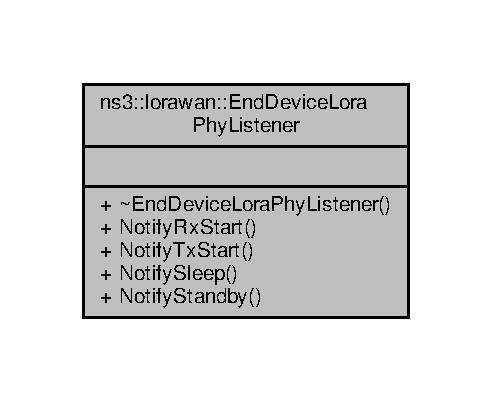
\includegraphics[width=236pt]{classns3_1_1lorawan_1_1EndDeviceLoraPhyListener__coll__graph}
\end{center}
\end{figure}
\subsection*{Public Member Functions}
\begin{DoxyCompactItemize}
\item 
virtual void \hyperlink{classns3_1_1lorawan_1_1EndDeviceLoraPhyListener_acb82563f9dc6082e442c0ec6b1d32d94}{Notify\+Rx\+Start} ()=0
\item 
virtual void \hyperlink{classns3_1_1lorawan_1_1EndDeviceLoraPhyListener_abf3943484dc182ade9f180cd806d43f4}{Notify\+Tx\+Start} (double tx\+Power\+Dbm)=0
\item 
virtual void \hyperlink{classns3_1_1lorawan_1_1EndDeviceLoraPhyListener_a0e9d774b67cbddee98c5f7d76c844c65}{Notify\+Sleep} (void)=0
\item 
virtual void \hyperlink{classns3_1_1lorawan_1_1EndDeviceLoraPhyListener_ab7e6540205cc6a0cefbe226bda967187}{Notify\+Standby} (void)=0
\end{DoxyCompactItemize}


\subsection{Detailed Description}
Receive notifications about P\+HY events. 

\subsection{Member Function Documentation}
\mbox{\Hypertarget{classns3_1_1lorawan_1_1EndDeviceLoraPhyListener_acb82563f9dc6082e442c0ec6b1d32d94}\label{classns3_1_1lorawan_1_1EndDeviceLoraPhyListener_acb82563f9dc6082e442c0ec6b1d32d94}} 
\index{ns3\+::lorawan\+::\+End\+Device\+Lora\+Phy\+Listener@{ns3\+::lorawan\+::\+End\+Device\+Lora\+Phy\+Listener}!Notify\+Rx\+Start@{Notify\+Rx\+Start}}
\index{Notify\+Rx\+Start@{Notify\+Rx\+Start}!ns3\+::lorawan\+::\+End\+Device\+Lora\+Phy\+Listener@{ns3\+::lorawan\+::\+End\+Device\+Lora\+Phy\+Listener}}
\subsubsection{\texorpdfstring{Notify\+Rx\+Start()}{NotifyRxStart()}}
{\footnotesize\ttfamily virtual void ns3\+::lorawan\+::\+End\+Device\+Lora\+Phy\+Listener\+::\+Notify\+Rx\+Start (\begin{DoxyParamCaption}{ }\end{DoxyParamCaption})\hspace{0.3cm}{\ttfamily [pure virtual]}}

We have received the first bit of a packet. We decided that we could synchronize on this packet. It does not mean we will be able to successfully receive completely the whole packet. It means that we will report a B\+U\+SY status until one of the following happens\+:
\begin{DoxyItemize}
\item Notify\+Rx\+End\+Ok
\item Notify\+Rx\+End\+Error
\item Notify\+Tx\+Start
\end{DoxyItemize}


\begin{DoxyParams}{Parameters}
{\em duration} & the expected duration of the packet reception. \\
\hline
\end{DoxyParams}


Implemented in \hyperlink{classns3_1_1lorawan_1_1LoraRadioEnergyModelPhyListener_a34bb7b2aae72cd8634672bd460247edb}{ns3\+::lorawan\+::\+Lora\+Radio\+Energy\+Model\+Phy\+Listener}.

\mbox{\Hypertarget{classns3_1_1lorawan_1_1EndDeviceLoraPhyListener_a0e9d774b67cbddee98c5f7d76c844c65}\label{classns3_1_1lorawan_1_1EndDeviceLoraPhyListener_a0e9d774b67cbddee98c5f7d76c844c65}} 
\index{ns3\+::lorawan\+::\+End\+Device\+Lora\+Phy\+Listener@{ns3\+::lorawan\+::\+End\+Device\+Lora\+Phy\+Listener}!Notify\+Sleep@{Notify\+Sleep}}
\index{Notify\+Sleep@{Notify\+Sleep}!ns3\+::lorawan\+::\+End\+Device\+Lora\+Phy\+Listener@{ns3\+::lorawan\+::\+End\+Device\+Lora\+Phy\+Listener}}
\subsubsection{\texorpdfstring{Notify\+Sleep()}{NotifySleep()}}
{\footnotesize\ttfamily virtual void ns3\+::lorawan\+::\+End\+Device\+Lora\+Phy\+Listener\+::\+Notify\+Sleep (\begin{DoxyParamCaption}\item[{void}]{ }\end{DoxyParamCaption})\hspace{0.3cm}{\ttfamily [pure virtual]}}

Notify listeners that we went to sleep 

Implemented in \hyperlink{classns3_1_1lorawan_1_1LoraRadioEnergyModelPhyListener_ac4e0739b8ae8f0ed5a94eb8c5e830641}{ns3\+::lorawan\+::\+Lora\+Radio\+Energy\+Model\+Phy\+Listener}.

\mbox{\Hypertarget{classns3_1_1lorawan_1_1EndDeviceLoraPhyListener_ab7e6540205cc6a0cefbe226bda967187}\label{classns3_1_1lorawan_1_1EndDeviceLoraPhyListener_ab7e6540205cc6a0cefbe226bda967187}} 
\index{ns3\+::lorawan\+::\+End\+Device\+Lora\+Phy\+Listener@{ns3\+::lorawan\+::\+End\+Device\+Lora\+Phy\+Listener}!Notify\+Standby@{Notify\+Standby}}
\index{Notify\+Standby@{Notify\+Standby}!ns3\+::lorawan\+::\+End\+Device\+Lora\+Phy\+Listener@{ns3\+::lorawan\+::\+End\+Device\+Lora\+Phy\+Listener}}
\subsubsection{\texorpdfstring{Notify\+Standby()}{NotifyStandby()}}
{\footnotesize\ttfamily virtual void ns3\+::lorawan\+::\+End\+Device\+Lora\+Phy\+Listener\+::\+Notify\+Standby (\begin{DoxyParamCaption}\item[{void}]{ }\end{DoxyParamCaption})\hspace{0.3cm}{\ttfamily [pure virtual]}}

Notify listeners that we woke up 

Implemented in \hyperlink{classns3_1_1lorawan_1_1LoraRadioEnergyModelPhyListener_ad5ce1283ba5c34384307338c24446876}{ns3\+::lorawan\+::\+Lora\+Radio\+Energy\+Model\+Phy\+Listener}.

\mbox{\Hypertarget{classns3_1_1lorawan_1_1EndDeviceLoraPhyListener_abf3943484dc182ade9f180cd806d43f4}\label{classns3_1_1lorawan_1_1EndDeviceLoraPhyListener_abf3943484dc182ade9f180cd806d43f4}} 
\index{ns3\+::lorawan\+::\+End\+Device\+Lora\+Phy\+Listener@{ns3\+::lorawan\+::\+End\+Device\+Lora\+Phy\+Listener}!Notify\+Tx\+Start@{Notify\+Tx\+Start}}
\index{Notify\+Tx\+Start@{Notify\+Tx\+Start}!ns3\+::lorawan\+::\+End\+Device\+Lora\+Phy\+Listener@{ns3\+::lorawan\+::\+End\+Device\+Lora\+Phy\+Listener}}
\subsubsection{\texorpdfstring{Notify\+Tx\+Start()}{NotifyTxStart()}}
{\footnotesize\ttfamily virtual void ns3\+::lorawan\+::\+End\+Device\+Lora\+Phy\+Listener\+::\+Notify\+Tx\+Start (\begin{DoxyParamCaption}\item[{double}]{tx\+Power\+Dbm }\end{DoxyParamCaption})\hspace{0.3cm}{\ttfamily [pure virtual]}}

We are about to send the first bit of the packet. We do not send any event to notify the end of transmission. Listeners should assume that the channel implicitely reverts to the idle state unless they have received a cca busy report.


\begin{DoxyParams}{Parameters}
{\em duration} & the expected transmission duration. \\
\hline
{\em tx\+Power\+Dbm} & the nominal tx power in d\+Bm \\
\hline
\end{DoxyParams}


Implemented in \hyperlink{classns3_1_1lorawan_1_1LoraRadioEnergyModelPhyListener_a42d031fca675ad2a5b76977a7d79e900}{ns3\+::lorawan\+::\+Lora\+Radio\+Energy\+Model\+Phy\+Listener}.



The documentation for this class was generated from the following files\+:\begin{DoxyCompactItemize}
\item 
end-\/device-\/lora-\/phy.\+h\item 
end-\/device-\/lora-\/phy.\+cc\end{DoxyCompactItemize}

\hypertarget{classns3_1_1lorawan_1_1EndDeviceStatus}{}\section{ns3\+:\+:lorawan\+:\+:End\+Device\+Status Class Reference}
\label{classns3_1_1lorawan_1_1EndDeviceStatus}\index{ns3\+::lorawan\+::\+End\+Device\+Status@{ns3\+::lorawan\+::\+End\+Device\+Status}}


{\ttfamily \#include $<$end-\/device-\/status.\+h$>$}



Inheritance diagram for ns3\+:\+:lorawan\+:\+:End\+Device\+Status\+:
\nopagebreak
\begin{figure}[H]
\begin{center}
\leavevmode
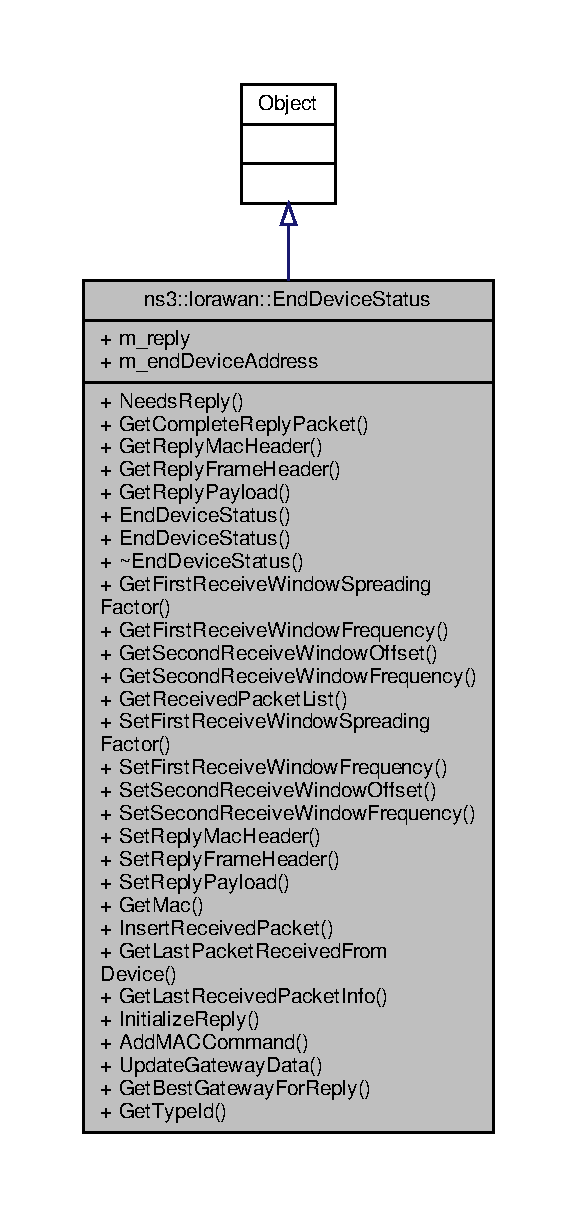
\includegraphics[height=550pt]{classns3_1_1lorawan_1_1EndDeviceStatus__inherit__graph}
\end{center}
\end{figure}


Collaboration diagram for ns3\+:\+:lorawan\+:\+:End\+Device\+Status\+:
\nopagebreak
\begin{figure}[H]
\begin{center}
\leavevmode
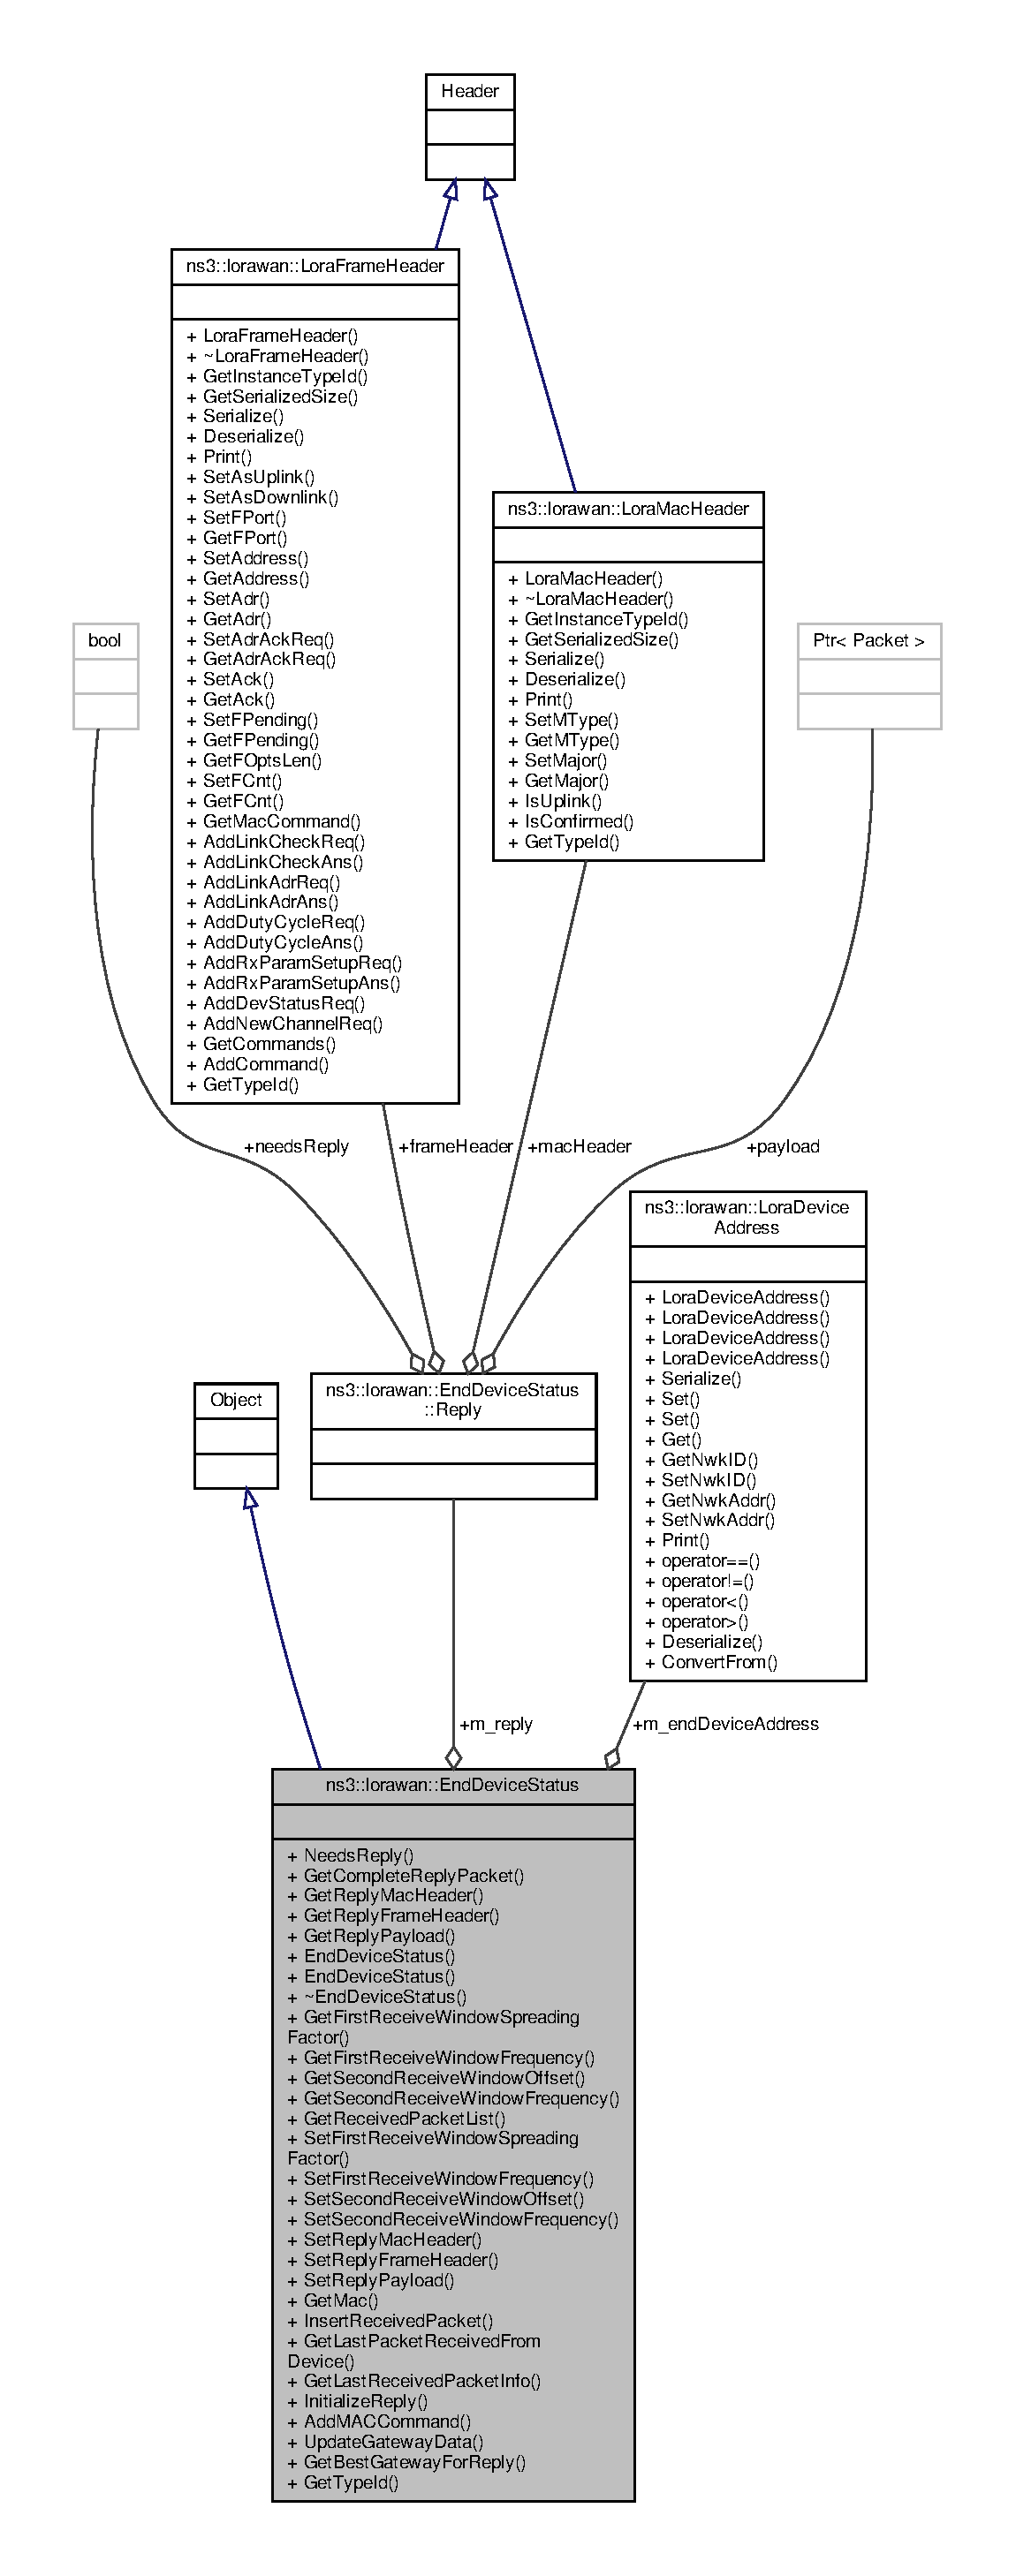
\includegraphics[height=550pt]{classns3_1_1lorawan_1_1EndDeviceStatus__coll__graph}
\end{center}
\end{figure}
\subsection*{Classes}
\begin{DoxyCompactItemize}
\item 
struct \hyperlink{structns3_1_1lorawan_1_1EndDeviceStatus_1_1PacketInfoPerGw}{Packet\+Info\+Per\+Gw}
\item 
struct \hyperlink{structns3_1_1lorawan_1_1EndDeviceStatus_1_1ReceivedPacketInfo}{Received\+Packet\+Info}
\item 
struct \hyperlink{structns3_1_1lorawan_1_1EndDeviceStatus_1_1Reply}{Reply}
\end{DoxyCompactItemize}
\subsection*{Public Types}
\begin{DoxyCompactItemize}
\item 
\mbox{\Hypertarget{classns3_1_1lorawan_1_1EndDeviceStatus_a85bd7a844d001f0a3e04d14165e3be70}\label{classns3_1_1lorawan_1_1EndDeviceStatus_a85bd7a844d001f0a3e04d14165e3be70}} 
typedef std\+::map$<$ Address, \hyperlink{structns3_1_1lorawan_1_1EndDeviceStatus_1_1PacketInfoPerGw}{Packet\+Info\+Per\+Gw} $>$ {\bfseries Gateway\+List}
\item 
\mbox{\Hypertarget{classns3_1_1lorawan_1_1EndDeviceStatus_a081d59ec2c06b37e925710efca555da0}\label{classns3_1_1lorawan_1_1EndDeviceStatus_a081d59ec2c06b37e925710efca555da0}} 
typedef std\+::list$<$ std\+::pair$<$ Ptr$<$ Packet const  $>$, \hyperlink{structns3_1_1lorawan_1_1EndDeviceStatus_1_1ReceivedPacketInfo}{Received\+Packet\+Info} $>$ $>$ {\bfseries Received\+Packet\+List}
\end{DoxyCompactItemize}
\subsection*{Public Member Functions}
\begin{DoxyCompactItemize}
\item 
bool \hyperlink{classns3_1_1lorawan_1_1EndDeviceStatus_a25e0c2769696c42a5e62088b2ba0bb2a}{Needs\+Reply} (void)
\item 
Ptr$<$ Packet $>$ \hyperlink{classns3_1_1lorawan_1_1EndDeviceStatus_a816b1769aefdd36fdc06f8f2a5af34f3}{Get\+Complete\+Reply\+Packet} (void)
\item 
\hyperlink{classns3_1_1lorawan_1_1LoraMacHeader}{Lora\+Mac\+Header} \hyperlink{classns3_1_1lorawan_1_1EndDeviceStatus_aec276e89a9a780dce296822f3f7b25b9}{Get\+Reply\+Mac\+Header} (void)
\item 
\hyperlink{classns3_1_1lorawan_1_1LoraFrameHeader}{Lora\+Frame\+Header} \hyperlink{classns3_1_1lorawan_1_1EndDeviceStatus_af2095509552ac48da422cbd14f7e975b}{Get\+Reply\+Frame\+Header} (void)
\item 
Ptr$<$ Packet $>$ \hyperlink{classns3_1_1lorawan_1_1EndDeviceStatus_a718b9f8457df5793a03d9442a4ffed60}{Get\+Reply\+Payload} (void)
\item 
\mbox{\Hypertarget{classns3_1_1lorawan_1_1EndDeviceStatus_adb0f7234e45ea0051e26c6d8bc323c75}\label{classns3_1_1lorawan_1_1EndDeviceStatus_adb0f7234e45ea0051e26c6d8bc323c75}} 
{\bfseries End\+Device\+Status} (\hyperlink{classns3_1_1lorawan_1_1LoraDeviceAddress}{Lora\+Device\+Address} end\+Device\+Address, Ptr$<$ \hyperlink{classns3_1_1lorawan_1_1EndDeviceLoraMac}{End\+Device\+Lora\+Mac} $>$ end\+Device\+Mac)
\item 
uint8\+\_\+t \hyperlink{classns3_1_1lorawan_1_1EndDeviceStatus_aff3f9a544427d61022b526f2a131d614}{Get\+First\+Receive\+Window\+Spreading\+Factor} (void)
\item 
double \hyperlink{classns3_1_1lorawan_1_1EndDeviceStatus_afdb51088fb0af238160ba8bfec7bf0de}{Get\+First\+Receive\+Window\+Frequency} (void)
\item 
uint8\+\_\+t \hyperlink{classns3_1_1lorawan_1_1EndDeviceStatus_a9dc3c9107e16f19ccf96e462c01d1fe3}{Get\+Second\+Receive\+Window\+Offset} (void)
\item 
double \hyperlink{classns3_1_1lorawan_1_1EndDeviceStatus_a29a72fd91a4cd5ea1d4010ba990ec5b6}{Get\+Second\+Receive\+Window\+Frequency} (void)
\item 
Received\+Packet\+List \hyperlink{classns3_1_1lorawan_1_1EndDeviceStatus_af0ea395ca783b6bd3d55fc8f5cba704d}{Get\+Received\+Packet\+List} (void)
\item 
void \hyperlink{classns3_1_1lorawan_1_1EndDeviceStatus_ac39c49bf91b1bcdbf08add2694bca011}{Set\+First\+Receive\+Window\+Spreading\+Factor} (uint8\+\_\+t sf)
\item 
void \hyperlink{classns3_1_1lorawan_1_1EndDeviceStatus_a0a5445bfba22ce6dd318128eb4e8bc59}{Set\+First\+Receive\+Window\+Frequency} (double frequency)
\item 
void \hyperlink{classns3_1_1lorawan_1_1EndDeviceStatus_ac901c8879c93c79c7cc6fae82cb14909}{Set\+Second\+Receive\+Window\+Offset} (uint8\+\_\+t offset)
\item 
void \hyperlink{classns3_1_1lorawan_1_1EndDeviceStatus_a19b88dd518ed0885f7e4a59a5cd3feb7}{Set\+Second\+Receive\+Window\+Frequency} (double frequency)
\item 
void \hyperlink{classns3_1_1lorawan_1_1EndDeviceStatus_a68017acffb75ff0ccf70347dcd325b84}{Set\+Reply\+Mac\+Header} (\hyperlink{classns3_1_1lorawan_1_1LoraMacHeader}{Lora\+Mac\+Header} mac\+Header)
\item 
void \hyperlink{classns3_1_1lorawan_1_1EndDeviceStatus_a2f8b9b43a6d4b3af2be53777877e6787}{Set\+Reply\+Frame\+Header} (\hyperlink{classns3_1_1lorawan_1_1LoraFrameHeader}{Lora\+Frame\+Header} frame\+Header)
\item 
void \hyperlink{classns3_1_1lorawan_1_1EndDeviceStatus_aa21d19b3898ae972c644ec94993813ec}{Set\+Reply\+Payload} (Ptr$<$ Packet $>$ reply\+Payload)
\item 
\mbox{\Hypertarget{classns3_1_1lorawan_1_1EndDeviceStatus_a4fee5c291db27d3656ef5268b5e31137}\label{classns3_1_1lorawan_1_1EndDeviceStatus_a4fee5c291db27d3656ef5268b5e31137}} 
Ptr$<$ \hyperlink{classns3_1_1lorawan_1_1EndDeviceLoraMac}{End\+Device\+Lora\+Mac} $>$ {\bfseries Get\+Mac} (void)
\item 
void \hyperlink{classns3_1_1lorawan_1_1EndDeviceStatus_a57c324b1fc3708fab5b3a6c638226d91}{Insert\+Received\+Packet} (Ptr$<$ Packet const $>$ received\+Packet, const Address \&gw\+Address)
\item 
Ptr$<$ Packet const  $>$ \hyperlink{classns3_1_1lorawan_1_1EndDeviceStatus_ab4ead237afea3a967bced521bc474e47}{Get\+Last\+Packet\+Received\+From\+Device} (void)
\item 
\hyperlink{structns3_1_1lorawan_1_1EndDeviceStatus_1_1ReceivedPacketInfo}{End\+Device\+Status\+::\+Received\+Packet\+Info} \hyperlink{classns3_1_1lorawan_1_1EndDeviceStatus_a282dab8b89f752ae913e22d348b24c3f}{Get\+Last\+Received\+Packet\+Info} (void)
\item 
void \hyperlink{classns3_1_1lorawan_1_1EndDeviceStatus_a9d25dab867d40f0ef85881527d3467e8}{Initialize\+Reply} (void)
\item 
void \hyperlink{classns3_1_1lorawan_1_1EndDeviceStatus_ab9a84efe386e3677ecf9c817ba936dda}{Add\+M\+A\+C\+Command} (Ptr$<$ \hyperlink{classns3_1_1lorawan_1_1MacCommand}{Mac\+Command} $>$ mac\+Command)
\item 
void \hyperlink{classns3_1_1lorawan_1_1EndDeviceStatus_a1cd60fc88eb88c1990f28e8aee71e05f}{Update\+Gateway\+Data} (Gateway\+List gw\+List, Address gw\+Address, double rcv\+Power)
\item 
Address \hyperlink{classns3_1_1lorawan_1_1EndDeviceStatus_a08f78817278989d57c515af97b9b9204}{Get\+Best\+Gateway\+For\+Reply} (void)
\end{DoxyCompactItemize}
\subsection*{Static Public Member Functions}
\begin{DoxyCompactItemize}
\item 
\mbox{\Hypertarget{classns3_1_1lorawan_1_1EndDeviceStatus_af8792a24e34cc46530849ebcaa9896e1}\label{classns3_1_1lorawan_1_1EndDeviceStatus_af8792a24e34cc46530849ebcaa9896e1}} 
static Type\+Id {\bfseries Get\+Type\+Id} (void)
\end{DoxyCompactItemize}
\subsection*{Public Attributes}
\begin{DoxyCompactItemize}
\item 
\mbox{\Hypertarget{classns3_1_1lorawan_1_1EndDeviceStatus_a5ff004b81ff7c6d555bbe670c42bec0b}\label{classns3_1_1lorawan_1_1EndDeviceStatus_a5ff004b81ff7c6d555bbe670c42bec0b}} 
struct \hyperlink{structns3_1_1lorawan_1_1EndDeviceStatus_1_1Reply}{Reply} {\bfseries m\+\_\+reply}
\item 
\mbox{\Hypertarget{classns3_1_1lorawan_1_1EndDeviceStatus_a60b7ba4fdaf30e9824f355beca66c617}\label{classns3_1_1lorawan_1_1EndDeviceStatus_a60b7ba4fdaf30e9824f355beca66c617}} 
\hyperlink{classns3_1_1lorawan_1_1LoraDeviceAddress}{Lora\+Device\+Address} {\bfseries m\+\_\+end\+Device\+Address}
\end{DoxyCompactItemize}
\subsection*{Friends}
\begin{DoxyCompactItemize}
\item 
\mbox{\Hypertarget{classns3_1_1lorawan_1_1EndDeviceStatus_a8b9f34fb2bce772f0a8887243ded0977}\label{classns3_1_1lorawan_1_1EndDeviceStatus_a8b9f34fb2bce772f0a8887243ded0977}} 
std\+::ostream \& {\bfseries operator$<$$<$} (std\+::ostream \&os, const \hyperlink{classns3_1_1lorawan_1_1EndDeviceStatus}{End\+Device\+Status} \&status)
\end{DoxyCompactItemize}


\subsection{Detailed Description}
This class represents the Network Server\textquotesingle{}s knowledge about an End Device in the Lo\+Ra\+W\+AN network it is administering.

The Network Server\textquotesingle{}s \hyperlink{classns3_1_1lorawan_1_1NetworkStatus}{Network\+Status} component contains a list of instances of this class, one for each device in the network. Each instance contains all the parameters and information of the end device and the packets received from it. Furthermore, this class holds the reply packet that the network server will send to this device at the first available receive window. Upon new packet arrivals at the Network Server, the On\+Received\+Packet method is called to update the information regarding the last received packet and its parameters. 

\subsection{Member Function Documentation}
\mbox{\Hypertarget{classns3_1_1lorawan_1_1EndDeviceStatus_ab9a84efe386e3677ecf9c817ba936dda}\label{classns3_1_1lorawan_1_1EndDeviceStatus_ab9a84efe386e3677ecf9c817ba936dda}} 
\index{ns3\+::lorawan\+::\+End\+Device\+Status@{ns3\+::lorawan\+::\+End\+Device\+Status}!Add\+M\+A\+C\+Command@{Add\+M\+A\+C\+Command}}
\index{Add\+M\+A\+C\+Command@{Add\+M\+A\+C\+Command}!ns3\+::lorawan\+::\+End\+Device\+Status@{ns3\+::lorawan\+::\+End\+Device\+Status}}
\subsubsection{\texorpdfstring{Add\+M\+A\+C\+Command()}{AddMACCommand()}}
{\footnotesize\ttfamily void ns3\+::lorawan\+::\+End\+Device\+Status\+::\+Add\+M\+A\+C\+Command (\begin{DoxyParamCaption}\item[{Ptr$<$ \hyperlink{classns3_1_1lorawan_1_1MacCommand}{Mac\+Command} $>$}]{mac\+Command }\end{DoxyParamCaption})}

Add M\+AC command to the list. \mbox{\Hypertarget{classns3_1_1lorawan_1_1EndDeviceStatus_a08f78817278989d57c515af97b9b9204}\label{classns3_1_1lorawan_1_1EndDeviceStatus_a08f78817278989d57c515af97b9b9204}} 
\index{ns3\+::lorawan\+::\+End\+Device\+Status@{ns3\+::lorawan\+::\+End\+Device\+Status}!Get\+Best\+Gateway\+For\+Reply@{Get\+Best\+Gateway\+For\+Reply}}
\index{Get\+Best\+Gateway\+For\+Reply@{Get\+Best\+Gateway\+For\+Reply}!ns3\+::lorawan\+::\+End\+Device\+Status@{ns3\+::lorawan\+::\+End\+Device\+Status}}
\subsubsection{\texorpdfstring{Get\+Best\+Gateway\+For\+Reply()}{GetBestGatewayForReply()}}
{\footnotesize\ttfamily Address ns3\+::lorawan\+::\+End\+Device\+Status\+::\+Get\+Best\+Gateway\+For\+Reply (\begin{DoxyParamCaption}\item[{void}]{ }\end{DoxyParamCaption})}

Return the best gateway that\+:
\begin{DoxyItemize}
\item Can reach this device
\item Is available to send a packet 
\end{DoxyItemize}\mbox{\Hypertarget{classns3_1_1lorawan_1_1EndDeviceStatus_a816b1769aefdd36fdc06f8f2a5af34f3}\label{classns3_1_1lorawan_1_1EndDeviceStatus_a816b1769aefdd36fdc06f8f2a5af34f3}} 
\index{ns3\+::lorawan\+::\+End\+Device\+Status@{ns3\+::lorawan\+::\+End\+Device\+Status}!Get\+Complete\+Reply\+Packet@{Get\+Complete\+Reply\+Packet}}
\index{Get\+Complete\+Reply\+Packet@{Get\+Complete\+Reply\+Packet}!ns3\+::lorawan\+::\+End\+Device\+Status@{ns3\+::lorawan\+::\+End\+Device\+Status}}
\subsubsection{\texorpdfstring{Get\+Complete\+Reply\+Packet()}{GetCompleteReplyPacket()}}
{\footnotesize\ttfamily Ptr$<$ Packet $>$ ns3\+::lorawan\+::\+End\+Device\+Status\+::\+Get\+Complete\+Reply\+Packet (\begin{DoxyParamCaption}\item[{void}]{ }\end{DoxyParamCaption})}

Get the reply packet.

\begin{DoxyReturn}{Returns}
A pointer to the packet reply (data + headers). 
\end{DoxyReturn}
\mbox{\Hypertarget{classns3_1_1lorawan_1_1EndDeviceStatus_afdb51088fb0af238160ba8bfec7bf0de}\label{classns3_1_1lorawan_1_1EndDeviceStatus_afdb51088fb0af238160ba8bfec7bf0de}} 
\index{ns3\+::lorawan\+::\+End\+Device\+Status@{ns3\+::lorawan\+::\+End\+Device\+Status}!Get\+First\+Receive\+Window\+Frequency@{Get\+First\+Receive\+Window\+Frequency}}
\index{Get\+First\+Receive\+Window\+Frequency@{Get\+First\+Receive\+Window\+Frequency}!ns3\+::lorawan\+::\+End\+Device\+Status@{ns3\+::lorawan\+::\+End\+Device\+Status}}
\subsubsection{\texorpdfstring{Get\+First\+Receive\+Window\+Frequency()}{GetFirstReceiveWindowFrequency()}}
{\footnotesize\ttfamily double ns3\+::lorawan\+::\+End\+Device\+Status\+::\+Get\+First\+Receive\+Window\+Frequency (\begin{DoxyParamCaption}\item[{void}]{ }\end{DoxyParamCaption})}

Get the first window frequency of this device. \mbox{\Hypertarget{classns3_1_1lorawan_1_1EndDeviceStatus_aff3f9a544427d61022b526f2a131d614}\label{classns3_1_1lorawan_1_1EndDeviceStatus_aff3f9a544427d61022b526f2a131d614}} 
\index{ns3\+::lorawan\+::\+End\+Device\+Status@{ns3\+::lorawan\+::\+End\+Device\+Status}!Get\+First\+Receive\+Window\+Spreading\+Factor@{Get\+First\+Receive\+Window\+Spreading\+Factor}}
\index{Get\+First\+Receive\+Window\+Spreading\+Factor@{Get\+First\+Receive\+Window\+Spreading\+Factor}!ns3\+::lorawan\+::\+End\+Device\+Status@{ns3\+::lorawan\+::\+End\+Device\+Status}}
\subsubsection{\texorpdfstring{Get\+First\+Receive\+Window\+Spreading\+Factor()}{GetFirstReceiveWindowSpreadingFactor()}}
{\footnotesize\ttfamily uint8\+\_\+t ns3\+::lorawan\+::\+End\+Device\+Status\+::\+Get\+First\+Receive\+Window\+Spreading\+Factor (\begin{DoxyParamCaption}\item[{void}]{ }\end{DoxyParamCaption})}

Get the spreading factor this device is using in the first receive window.

\begin{DoxyReturn}{Returns}
An unsigned 8-\/bit integer containing the spreading factor. 
\end{DoxyReturn}
\mbox{\Hypertarget{classns3_1_1lorawan_1_1EndDeviceStatus_ab4ead237afea3a967bced521bc474e47}\label{classns3_1_1lorawan_1_1EndDeviceStatus_ab4ead237afea3a967bced521bc474e47}} 
\index{ns3\+::lorawan\+::\+End\+Device\+Status@{ns3\+::lorawan\+::\+End\+Device\+Status}!Get\+Last\+Packet\+Received\+From\+Device@{Get\+Last\+Packet\+Received\+From\+Device}}
\index{Get\+Last\+Packet\+Received\+From\+Device@{Get\+Last\+Packet\+Received\+From\+Device}!ns3\+::lorawan\+::\+End\+Device\+Status@{ns3\+::lorawan\+::\+End\+Device\+Status}}
\subsubsection{\texorpdfstring{Get\+Last\+Packet\+Received\+From\+Device()}{GetLastPacketReceivedFromDevice()}}
{\footnotesize\ttfamily Ptr$<$ Packet const  $>$ ns3\+::lorawan\+::\+End\+Device\+Status\+::\+Get\+Last\+Packet\+Received\+From\+Device (\begin{DoxyParamCaption}\item[{void}]{ }\end{DoxyParamCaption})}

Return the last packet that was received from this device. \mbox{\Hypertarget{classns3_1_1lorawan_1_1EndDeviceStatus_a282dab8b89f752ae913e22d348b24c3f}\label{classns3_1_1lorawan_1_1EndDeviceStatus_a282dab8b89f752ae913e22d348b24c3f}} 
\index{ns3\+::lorawan\+::\+End\+Device\+Status@{ns3\+::lorawan\+::\+End\+Device\+Status}!Get\+Last\+Received\+Packet\+Info@{Get\+Last\+Received\+Packet\+Info}}
\index{Get\+Last\+Received\+Packet\+Info@{Get\+Last\+Received\+Packet\+Info}!ns3\+::lorawan\+::\+End\+Device\+Status@{ns3\+::lorawan\+::\+End\+Device\+Status}}
\subsubsection{\texorpdfstring{Get\+Last\+Received\+Packet\+Info()}{GetLastReceivedPacketInfo()}}
{\footnotesize\ttfamily \hyperlink{structns3_1_1lorawan_1_1EndDeviceStatus_1_1ReceivedPacketInfo}{End\+Device\+Status\+::\+Received\+Packet\+Info} ns3\+::lorawan\+::\+End\+Device\+Status\+::\+Get\+Last\+Received\+Packet\+Info (\begin{DoxyParamCaption}\item[{void}]{ }\end{DoxyParamCaption})}

Return the information about the last packet that was received from the device. \mbox{\Hypertarget{classns3_1_1lorawan_1_1EndDeviceStatus_af0ea395ca783b6bd3d55fc8f5cba704d}\label{classns3_1_1lorawan_1_1EndDeviceStatus_af0ea395ca783b6bd3d55fc8f5cba704d}} 
\index{ns3\+::lorawan\+::\+End\+Device\+Status@{ns3\+::lorawan\+::\+End\+Device\+Status}!Get\+Received\+Packet\+List@{Get\+Received\+Packet\+List}}
\index{Get\+Received\+Packet\+List@{Get\+Received\+Packet\+List}!ns3\+::lorawan\+::\+End\+Device\+Status@{ns3\+::lorawan\+::\+End\+Device\+Status}}
\subsubsection{\texorpdfstring{Get\+Received\+Packet\+List()}{GetReceivedPacketList()}}
{\footnotesize\ttfamily End\+Device\+Status\+::\+Received\+Packet\+List ns3\+::lorawan\+::\+End\+Device\+Status\+::\+Get\+Received\+Packet\+List (\begin{DoxyParamCaption}\item[{void}]{ }\end{DoxyParamCaption})}

Get the received packet list.

\begin{DoxyReturn}{Returns}
The received packet list. 
\end{DoxyReturn}
\mbox{\Hypertarget{classns3_1_1lorawan_1_1EndDeviceStatus_af2095509552ac48da422cbd14f7e975b}\label{classns3_1_1lorawan_1_1EndDeviceStatus_af2095509552ac48da422cbd14f7e975b}} 
\index{ns3\+::lorawan\+::\+End\+Device\+Status@{ns3\+::lorawan\+::\+End\+Device\+Status}!Get\+Reply\+Frame\+Header@{Get\+Reply\+Frame\+Header}}
\index{Get\+Reply\+Frame\+Header@{Get\+Reply\+Frame\+Header}!ns3\+::lorawan\+::\+End\+Device\+Status@{ns3\+::lorawan\+::\+End\+Device\+Status}}
\subsubsection{\texorpdfstring{Get\+Reply\+Frame\+Header()}{GetReplyFrameHeader()}}
{\footnotesize\ttfamily \hyperlink{classns3_1_1lorawan_1_1LoraFrameHeader}{Lora\+Frame\+Header} ns3\+::lorawan\+::\+End\+Device\+Status\+::\+Get\+Reply\+Frame\+Header (\begin{DoxyParamCaption}\item[{void}]{ }\end{DoxyParamCaption})}

Get the reply packet frame header.

\begin{DoxyReturn}{Returns}
The packet reply frame header. 
\end{DoxyReturn}
\mbox{\Hypertarget{classns3_1_1lorawan_1_1EndDeviceStatus_aec276e89a9a780dce296822f3f7b25b9}\label{classns3_1_1lorawan_1_1EndDeviceStatus_aec276e89a9a780dce296822f3f7b25b9}} 
\index{ns3\+::lorawan\+::\+End\+Device\+Status@{ns3\+::lorawan\+::\+End\+Device\+Status}!Get\+Reply\+Mac\+Header@{Get\+Reply\+Mac\+Header}}
\index{Get\+Reply\+Mac\+Header@{Get\+Reply\+Mac\+Header}!ns3\+::lorawan\+::\+End\+Device\+Status@{ns3\+::lorawan\+::\+End\+Device\+Status}}
\subsubsection{\texorpdfstring{Get\+Reply\+Mac\+Header()}{GetReplyMacHeader()}}
{\footnotesize\ttfamily \hyperlink{classns3_1_1lorawan_1_1LoraMacHeader}{Lora\+Mac\+Header} ns3\+::lorawan\+::\+End\+Device\+Status\+::\+Get\+Reply\+Mac\+Header (\begin{DoxyParamCaption}\item[{void}]{ }\end{DoxyParamCaption})}

Get the reply packet mac header.

\begin{DoxyReturn}{Returns}
The packet reply mac header. 
\end{DoxyReturn}
\mbox{\Hypertarget{classns3_1_1lorawan_1_1EndDeviceStatus_a718b9f8457df5793a03d9442a4ffed60}\label{classns3_1_1lorawan_1_1EndDeviceStatus_a718b9f8457df5793a03d9442a4ffed60}} 
\index{ns3\+::lorawan\+::\+End\+Device\+Status@{ns3\+::lorawan\+::\+End\+Device\+Status}!Get\+Reply\+Payload@{Get\+Reply\+Payload}}
\index{Get\+Reply\+Payload@{Get\+Reply\+Payload}!ns3\+::lorawan\+::\+End\+Device\+Status@{ns3\+::lorawan\+::\+End\+Device\+Status}}
\subsubsection{\texorpdfstring{Get\+Reply\+Payload()}{GetReplyPayload()}}
{\footnotesize\ttfamily Ptr$<$ Packet $>$ ns3\+::lorawan\+::\+End\+Device\+Status\+::\+Get\+Reply\+Payload (\begin{DoxyParamCaption}\item[{void}]{ }\end{DoxyParamCaption})}

Get the data of the reply packet.

\begin{DoxyReturn}{Returns}
A pointer to the packet reply. 
\end{DoxyReturn}
\mbox{\Hypertarget{classns3_1_1lorawan_1_1EndDeviceStatus_a29a72fd91a4cd5ea1d4010ba990ec5b6}\label{classns3_1_1lorawan_1_1EndDeviceStatus_a29a72fd91a4cd5ea1d4010ba990ec5b6}} 
\index{ns3\+::lorawan\+::\+End\+Device\+Status@{ns3\+::lorawan\+::\+End\+Device\+Status}!Get\+Second\+Receive\+Window\+Frequency@{Get\+Second\+Receive\+Window\+Frequency}}
\index{Get\+Second\+Receive\+Window\+Frequency@{Get\+Second\+Receive\+Window\+Frequency}!ns3\+::lorawan\+::\+End\+Device\+Status@{ns3\+::lorawan\+::\+End\+Device\+Status}}
\subsubsection{\texorpdfstring{Get\+Second\+Receive\+Window\+Frequency()}{GetSecondReceiveWindowFrequency()}}
{\footnotesize\ttfamily double ns3\+::lorawan\+::\+End\+Device\+Status\+::\+Get\+Second\+Receive\+Window\+Frequency (\begin{DoxyParamCaption}\item[{void}]{ }\end{DoxyParamCaption})}

Return the second window frequency of this device. \mbox{\Hypertarget{classns3_1_1lorawan_1_1EndDeviceStatus_a9dc3c9107e16f19ccf96e462c01d1fe3}\label{classns3_1_1lorawan_1_1EndDeviceStatus_a9dc3c9107e16f19ccf96e462c01d1fe3}} 
\index{ns3\+::lorawan\+::\+End\+Device\+Status@{ns3\+::lorawan\+::\+End\+Device\+Status}!Get\+Second\+Receive\+Window\+Offset@{Get\+Second\+Receive\+Window\+Offset}}
\index{Get\+Second\+Receive\+Window\+Offset@{Get\+Second\+Receive\+Window\+Offset}!ns3\+::lorawan\+::\+End\+Device\+Status@{ns3\+::lorawan\+::\+End\+Device\+Status}}
\subsubsection{\texorpdfstring{Get\+Second\+Receive\+Window\+Offset()}{GetSecondReceiveWindowOffset()}}
{\footnotesize\ttfamily uint8\+\_\+t ns3\+::lorawan\+::\+End\+Device\+Status\+::\+Get\+Second\+Receive\+Window\+Offset (\begin{DoxyParamCaption}\item[{void}]{ }\end{DoxyParamCaption})}

Get the offset of spreading factor this device is using in the second receive window with respect to the first receive window.

\begin{DoxyReturn}{Returns}
An unsigned 8-\/bit integer containing the spreading factor. 
\end{DoxyReturn}
\mbox{\Hypertarget{classns3_1_1lorawan_1_1EndDeviceStatus_a9d25dab867d40f0ef85881527d3467e8}\label{classns3_1_1lorawan_1_1EndDeviceStatus_a9d25dab867d40f0ef85881527d3467e8}} 
\index{ns3\+::lorawan\+::\+End\+Device\+Status@{ns3\+::lorawan\+::\+End\+Device\+Status}!Initialize\+Reply@{Initialize\+Reply}}
\index{Initialize\+Reply@{Initialize\+Reply}!ns3\+::lorawan\+::\+End\+Device\+Status@{ns3\+::lorawan\+::\+End\+Device\+Status}}
\subsubsection{\texorpdfstring{Initialize\+Reply()}{InitializeReply()}}
{\footnotesize\ttfamily void ns3\+::lorawan\+::\+End\+Device\+Status\+::\+Initialize\+Reply (\begin{DoxyParamCaption}\item[{void}]{ }\end{DoxyParamCaption})}

Initialize reply. \mbox{\Hypertarget{classns3_1_1lorawan_1_1EndDeviceStatus_a57c324b1fc3708fab5b3a6c638226d91}\label{classns3_1_1lorawan_1_1EndDeviceStatus_a57c324b1fc3708fab5b3a6c638226d91}} 
\index{ns3\+::lorawan\+::\+End\+Device\+Status@{ns3\+::lorawan\+::\+End\+Device\+Status}!Insert\+Received\+Packet@{Insert\+Received\+Packet}}
\index{Insert\+Received\+Packet@{Insert\+Received\+Packet}!ns3\+::lorawan\+::\+End\+Device\+Status@{ns3\+::lorawan\+::\+End\+Device\+Status}}
\subsubsection{\texorpdfstring{Insert\+Received\+Packet()}{InsertReceivedPacket()}}
{\footnotesize\ttfamily void ns3\+::lorawan\+::\+End\+Device\+Status\+::\+Insert\+Received\+Packet (\begin{DoxyParamCaption}\item[{Ptr$<$ Packet const $>$}]{received\+Packet,  }\item[{const Address \&}]{gw\+Address }\end{DoxyParamCaption})}

Insert a received packet in the packet list. \mbox{\Hypertarget{classns3_1_1lorawan_1_1EndDeviceStatus_a25e0c2769696c42a5e62088b2ba0bb2a}\label{classns3_1_1lorawan_1_1EndDeviceStatus_a25e0c2769696c42a5e62088b2ba0bb2a}} 
\index{ns3\+::lorawan\+::\+End\+Device\+Status@{ns3\+::lorawan\+::\+End\+Device\+Status}!Needs\+Reply@{Needs\+Reply}}
\index{Needs\+Reply@{Needs\+Reply}!ns3\+::lorawan\+::\+End\+Device\+Status@{ns3\+::lorawan\+::\+End\+Device\+Status}}
\subsubsection{\texorpdfstring{Needs\+Reply()}{NeedsReply()}}
{\footnotesize\ttfamily bool ns3\+::lorawan\+::\+End\+Device\+Status\+::\+Needs\+Reply (\begin{DoxyParamCaption}\item[{void}]{ }\end{DoxyParamCaption})}

Whether the end device needs a reply.

This is determined by looking at headers and payload of the \hyperlink{structns3_1_1lorawan_1_1EndDeviceStatus_1_1Reply}{Reply} structure\+: if they are empty, no reply should be needed.

\begin{DoxyReturn}{Returns}
A boolean value signaling if the end device needs a reply. 
\end{DoxyReturn}
\mbox{\Hypertarget{classns3_1_1lorawan_1_1EndDeviceStatus_a0a5445bfba22ce6dd318128eb4e8bc59}\label{classns3_1_1lorawan_1_1EndDeviceStatus_a0a5445bfba22ce6dd318128eb4e8bc59}} 
\index{ns3\+::lorawan\+::\+End\+Device\+Status@{ns3\+::lorawan\+::\+End\+Device\+Status}!Set\+First\+Receive\+Window\+Frequency@{Set\+First\+Receive\+Window\+Frequency}}
\index{Set\+First\+Receive\+Window\+Frequency@{Set\+First\+Receive\+Window\+Frequency}!ns3\+::lorawan\+::\+End\+Device\+Status@{ns3\+::lorawan\+::\+End\+Device\+Status}}
\subsubsection{\texorpdfstring{Set\+First\+Receive\+Window\+Frequency()}{SetFirstReceiveWindowFrequency()}}
{\footnotesize\ttfamily void ns3\+::lorawan\+::\+End\+Device\+Status\+::\+Set\+First\+Receive\+Window\+Frequency (\begin{DoxyParamCaption}\item[{double}]{frequency }\end{DoxyParamCaption})}

Set the first window frequency of this device. \mbox{\Hypertarget{classns3_1_1lorawan_1_1EndDeviceStatus_ac39c49bf91b1bcdbf08add2694bca011}\label{classns3_1_1lorawan_1_1EndDeviceStatus_ac39c49bf91b1bcdbf08add2694bca011}} 
\index{ns3\+::lorawan\+::\+End\+Device\+Status@{ns3\+::lorawan\+::\+End\+Device\+Status}!Set\+First\+Receive\+Window\+Spreading\+Factor@{Set\+First\+Receive\+Window\+Spreading\+Factor}}
\index{Set\+First\+Receive\+Window\+Spreading\+Factor@{Set\+First\+Receive\+Window\+Spreading\+Factor}!ns3\+::lorawan\+::\+End\+Device\+Status@{ns3\+::lorawan\+::\+End\+Device\+Status}}
\subsubsection{\texorpdfstring{Set\+First\+Receive\+Window\+Spreading\+Factor()}{SetFirstReceiveWindowSpreadingFactor()}}
{\footnotesize\ttfamily void ns3\+::lorawan\+::\+End\+Device\+Status\+::\+Set\+First\+Receive\+Window\+Spreading\+Factor (\begin{DoxyParamCaption}\item[{uint8\+\_\+t}]{sf }\end{DoxyParamCaption})}

Set the spreading factor this device is using in the first receive window. \mbox{\Hypertarget{classns3_1_1lorawan_1_1EndDeviceStatus_a2f8b9b43a6d4b3af2be53777877e6787}\label{classns3_1_1lorawan_1_1EndDeviceStatus_a2f8b9b43a6d4b3af2be53777877e6787}} 
\index{ns3\+::lorawan\+::\+End\+Device\+Status@{ns3\+::lorawan\+::\+End\+Device\+Status}!Set\+Reply\+Frame\+Header@{Set\+Reply\+Frame\+Header}}
\index{Set\+Reply\+Frame\+Header@{Set\+Reply\+Frame\+Header}!ns3\+::lorawan\+::\+End\+Device\+Status@{ns3\+::lorawan\+::\+End\+Device\+Status}}
\subsubsection{\texorpdfstring{Set\+Reply\+Frame\+Header()}{SetReplyFrameHeader()}}
{\footnotesize\ttfamily void ns3\+::lorawan\+::\+End\+Device\+Status\+::\+Set\+Reply\+Frame\+Header (\begin{DoxyParamCaption}\item[{\hyperlink{classns3_1_1lorawan_1_1LoraFrameHeader}{Lora\+Frame\+Header}}]{frame\+Header }\end{DoxyParamCaption})}

Set the reply packet frame header. \mbox{\Hypertarget{classns3_1_1lorawan_1_1EndDeviceStatus_a68017acffb75ff0ccf70347dcd325b84}\label{classns3_1_1lorawan_1_1EndDeviceStatus_a68017acffb75ff0ccf70347dcd325b84}} 
\index{ns3\+::lorawan\+::\+End\+Device\+Status@{ns3\+::lorawan\+::\+End\+Device\+Status}!Set\+Reply\+Mac\+Header@{Set\+Reply\+Mac\+Header}}
\index{Set\+Reply\+Mac\+Header@{Set\+Reply\+Mac\+Header}!ns3\+::lorawan\+::\+End\+Device\+Status@{ns3\+::lorawan\+::\+End\+Device\+Status}}
\subsubsection{\texorpdfstring{Set\+Reply\+Mac\+Header()}{SetReplyMacHeader()}}
{\footnotesize\ttfamily void ns3\+::lorawan\+::\+End\+Device\+Status\+::\+Set\+Reply\+Mac\+Header (\begin{DoxyParamCaption}\item[{\hyperlink{classns3_1_1lorawan_1_1LoraMacHeader}{Lora\+Mac\+Header}}]{mac\+Header }\end{DoxyParamCaption})}

Set the reply packet mac header. \mbox{\Hypertarget{classns3_1_1lorawan_1_1EndDeviceStatus_aa21d19b3898ae972c644ec94993813ec}\label{classns3_1_1lorawan_1_1EndDeviceStatus_aa21d19b3898ae972c644ec94993813ec}} 
\index{ns3\+::lorawan\+::\+End\+Device\+Status@{ns3\+::lorawan\+::\+End\+Device\+Status}!Set\+Reply\+Payload@{Set\+Reply\+Payload}}
\index{Set\+Reply\+Payload@{Set\+Reply\+Payload}!ns3\+::lorawan\+::\+End\+Device\+Status@{ns3\+::lorawan\+::\+End\+Device\+Status}}
\subsubsection{\texorpdfstring{Set\+Reply\+Payload()}{SetReplyPayload()}}
{\footnotesize\ttfamily void ns3\+::lorawan\+::\+End\+Device\+Status\+::\+Set\+Reply\+Payload (\begin{DoxyParamCaption}\item[{Ptr$<$ Packet $>$}]{reply\+Payload }\end{DoxyParamCaption})}

Set the packet reply payload. \mbox{\Hypertarget{classns3_1_1lorawan_1_1EndDeviceStatus_a19b88dd518ed0885f7e4a59a5cd3feb7}\label{classns3_1_1lorawan_1_1EndDeviceStatus_a19b88dd518ed0885f7e4a59a5cd3feb7}} 
\index{ns3\+::lorawan\+::\+End\+Device\+Status@{ns3\+::lorawan\+::\+End\+Device\+Status}!Set\+Second\+Receive\+Window\+Frequency@{Set\+Second\+Receive\+Window\+Frequency}}
\index{Set\+Second\+Receive\+Window\+Frequency@{Set\+Second\+Receive\+Window\+Frequency}!ns3\+::lorawan\+::\+End\+Device\+Status@{ns3\+::lorawan\+::\+End\+Device\+Status}}
\subsubsection{\texorpdfstring{Set\+Second\+Receive\+Window\+Frequency()}{SetSecondReceiveWindowFrequency()}}
{\footnotesize\ttfamily void ns3\+::lorawan\+::\+End\+Device\+Status\+::\+Set\+Second\+Receive\+Window\+Frequency (\begin{DoxyParamCaption}\item[{double}]{frequency }\end{DoxyParamCaption})}

Set the second window frequency of this device. \mbox{\Hypertarget{classns3_1_1lorawan_1_1EndDeviceStatus_ac901c8879c93c79c7cc6fae82cb14909}\label{classns3_1_1lorawan_1_1EndDeviceStatus_ac901c8879c93c79c7cc6fae82cb14909}} 
\index{ns3\+::lorawan\+::\+End\+Device\+Status@{ns3\+::lorawan\+::\+End\+Device\+Status}!Set\+Second\+Receive\+Window\+Offset@{Set\+Second\+Receive\+Window\+Offset}}
\index{Set\+Second\+Receive\+Window\+Offset@{Set\+Second\+Receive\+Window\+Offset}!ns3\+::lorawan\+::\+End\+Device\+Status@{ns3\+::lorawan\+::\+End\+Device\+Status}}
\subsubsection{\texorpdfstring{Set\+Second\+Receive\+Window\+Offset()}{SetSecondReceiveWindowOffset()}}
{\footnotesize\ttfamily void ns3\+::lorawan\+::\+End\+Device\+Status\+::\+Set\+Second\+Receive\+Window\+Offset (\begin{DoxyParamCaption}\item[{uint8\+\_\+t}]{offset }\end{DoxyParamCaption})}

Set the spreading factor this device is using in the first receive window. \mbox{\Hypertarget{classns3_1_1lorawan_1_1EndDeviceStatus_a1cd60fc88eb88c1990f28e8aee71e05f}\label{classns3_1_1lorawan_1_1EndDeviceStatus_a1cd60fc88eb88c1990f28e8aee71e05f}} 
\index{ns3\+::lorawan\+::\+End\+Device\+Status@{ns3\+::lorawan\+::\+End\+Device\+Status}!Update\+Gateway\+Data@{Update\+Gateway\+Data}}
\index{Update\+Gateway\+Data@{Update\+Gateway\+Data}!ns3\+::lorawan\+::\+End\+Device\+Status@{ns3\+::lorawan\+::\+End\+Device\+Status}}
\subsubsection{\texorpdfstring{Update\+Gateway\+Data()}{UpdateGatewayData()}}
{\footnotesize\ttfamily void ns3\+::lorawan\+::\+End\+Device\+Status\+::\+Update\+Gateway\+Data (\begin{DoxyParamCaption}\item[{Gateway\+List}]{gw\+List,  }\item[{Address}]{gw\+Address,  }\item[{double}]{rcv\+Power }\end{DoxyParamCaption})}

Update Gateway data when more then one gateway receive the same packet. 

The documentation for this class was generated from the following files\+:\begin{DoxyCompactItemize}
\item 
end-\/device-\/status.\+h\item 
end-\/device-\/status.\+cc\end{DoxyCompactItemize}

\hypertarget{classns3_1_1lorawan_1_1LoraInterferenceHelper_1_1Event}{}\section{ns3\+:\+:lorawan\+:\+:Lora\+Interference\+Helper\+:\+:Event Class Reference}
\label{classns3_1_1lorawan_1_1LoraInterferenceHelper_1_1Event}\index{ns3\+::lorawan\+::\+Lora\+Interference\+Helper\+::\+Event@{ns3\+::lorawan\+::\+Lora\+Interference\+Helper\+::\+Event}}


{\ttfamily \#include $<$lora-\/interference-\/helper.\+h$>$}



Inheritance diagram for ns3\+:\+:lorawan\+:\+:Lora\+Interference\+Helper\+:\+:Event\+:
\nopagebreak
\begin{figure}[H]
\begin{center}
\leavevmode
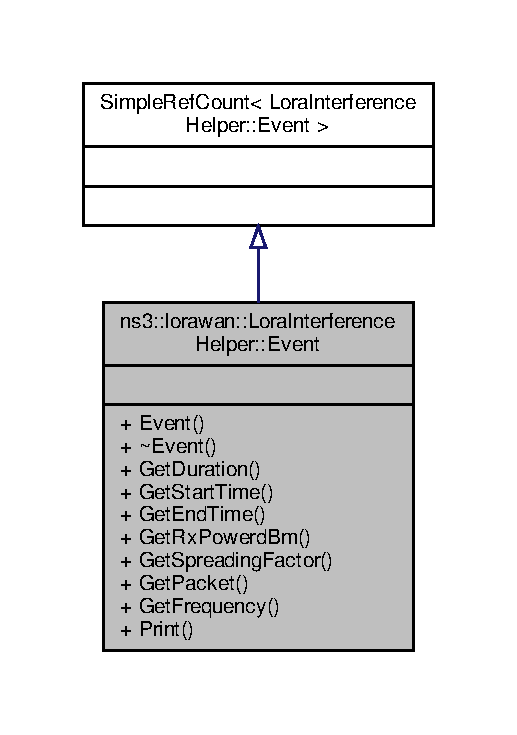
\includegraphics[width=248pt]{classns3_1_1lorawan_1_1LoraInterferenceHelper_1_1Event__inherit__graph}
\end{center}
\end{figure}


Collaboration diagram for ns3\+:\+:lorawan\+:\+:Lora\+Interference\+Helper\+:\+:Event\+:
\nopagebreak
\begin{figure}[H]
\begin{center}
\leavevmode
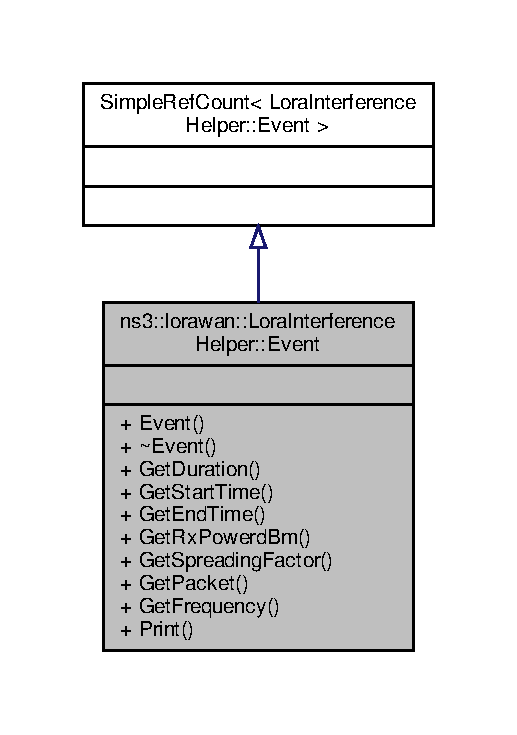
\includegraphics[width=248pt]{classns3_1_1lorawan_1_1LoraInterferenceHelper_1_1Event__coll__graph}
\end{center}
\end{figure}
\subsection*{Public Member Functions}
\begin{DoxyCompactItemize}
\item 
\mbox{\Hypertarget{classns3_1_1lorawan_1_1LoraInterferenceHelper_1_1Event_a7ed9e05bda1c59057d65d046d4982f39}\label{classns3_1_1lorawan_1_1LoraInterferenceHelper_1_1Event_a7ed9e05bda1c59057d65d046d4982f39}} 
{\bfseries Event} (Time duration, double rx\+Powerd\+Bm, uint8\+\_\+t spreading\+Factor, Ptr$<$ Packet $>$ packet, double frequency\+M\+Hz)
\item 
Time \hyperlink{classns3_1_1lorawan_1_1LoraInterferenceHelper_1_1Event_a1413175c6d325ae6e4131b3edc4df5aa}{Get\+Duration} (void) const
\item 
Time \hyperlink{classns3_1_1lorawan_1_1LoraInterferenceHelper_1_1Event_a0962fde4d6eca96401aea68a001d96fc}{Get\+Start\+Time} (void) const
\item 
Time \hyperlink{classns3_1_1lorawan_1_1LoraInterferenceHelper_1_1Event_a592178402fb4232513122ad3f9edcd0d}{Get\+End\+Time} (void) const
\item 
double \hyperlink{classns3_1_1lorawan_1_1LoraInterferenceHelper_1_1Event_a89d0371d6b9346699cad99be8d23e7aa}{Get\+Rx\+Powerd\+Bm} (void) const
\item 
uint8\+\_\+t \hyperlink{classns3_1_1lorawan_1_1LoraInterferenceHelper_1_1Event_af14d899b1e6f25dbe42b26824582085f}{Get\+Spreading\+Factor} (void) const
\item 
Ptr$<$ Packet $>$ \hyperlink{classns3_1_1lorawan_1_1LoraInterferenceHelper_1_1Event_ae1f0213b62e877c33ce3f37ca4f1f549}{Get\+Packet} (void) const
\item 
double \hyperlink{classns3_1_1lorawan_1_1LoraInterferenceHelper_1_1Event_a4dac36c337c87310c5820cc6571d9b5a}{Get\+Frequency} (void) const
\item 
void \hyperlink{classns3_1_1lorawan_1_1LoraInterferenceHelper_1_1Event_aa3a3f59131390caee329736d91748c93}{Print} (std\+::ostream \&stream) const
\end{DoxyCompactItemize}


\subsection{Detailed Description}
A class representing a signal in time.

Used in \hyperlink{classns3_1_1lorawan_1_1LoraInterferenceHelper}{Lora\+Interference\+Helper} to keep track of which signals overlap and cause destructive interference. 

\subsection{Member Function Documentation}
\mbox{\Hypertarget{classns3_1_1lorawan_1_1LoraInterferenceHelper_1_1Event_a1413175c6d325ae6e4131b3edc4df5aa}\label{classns3_1_1lorawan_1_1LoraInterferenceHelper_1_1Event_a1413175c6d325ae6e4131b3edc4df5aa}} 
\index{ns3\+::lorawan\+::\+Lora\+Interference\+Helper\+::\+Event@{ns3\+::lorawan\+::\+Lora\+Interference\+Helper\+::\+Event}!Get\+Duration@{Get\+Duration}}
\index{Get\+Duration@{Get\+Duration}!ns3\+::lorawan\+::\+Lora\+Interference\+Helper\+::\+Event@{ns3\+::lorawan\+::\+Lora\+Interference\+Helper\+::\+Event}}
\subsubsection{\texorpdfstring{Get\+Duration()}{GetDuration()}}
{\footnotesize\ttfamily Time ns3\+::lorawan\+::\+Lora\+Interference\+Helper\+::\+Event\+::\+Get\+Duration (\begin{DoxyParamCaption}\item[{void}]{ }\end{DoxyParamCaption}) const}

Get the duration of the event. \mbox{\Hypertarget{classns3_1_1lorawan_1_1LoraInterferenceHelper_1_1Event_a592178402fb4232513122ad3f9edcd0d}\label{classns3_1_1lorawan_1_1LoraInterferenceHelper_1_1Event_a592178402fb4232513122ad3f9edcd0d}} 
\index{ns3\+::lorawan\+::\+Lora\+Interference\+Helper\+::\+Event@{ns3\+::lorawan\+::\+Lora\+Interference\+Helper\+::\+Event}!Get\+End\+Time@{Get\+End\+Time}}
\index{Get\+End\+Time@{Get\+End\+Time}!ns3\+::lorawan\+::\+Lora\+Interference\+Helper\+::\+Event@{ns3\+::lorawan\+::\+Lora\+Interference\+Helper\+::\+Event}}
\subsubsection{\texorpdfstring{Get\+End\+Time()}{GetEndTime()}}
{\footnotesize\ttfamily Time ns3\+::lorawan\+::\+Lora\+Interference\+Helper\+::\+Event\+::\+Get\+End\+Time (\begin{DoxyParamCaption}\item[{void}]{ }\end{DoxyParamCaption}) const}

Get the ending time of the event. \mbox{\Hypertarget{classns3_1_1lorawan_1_1LoraInterferenceHelper_1_1Event_a4dac36c337c87310c5820cc6571d9b5a}\label{classns3_1_1lorawan_1_1LoraInterferenceHelper_1_1Event_a4dac36c337c87310c5820cc6571d9b5a}} 
\index{ns3\+::lorawan\+::\+Lora\+Interference\+Helper\+::\+Event@{ns3\+::lorawan\+::\+Lora\+Interference\+Helper\+::\+Event}!Get\+Frequency@{Get\+Frequency}}
\index{Get\+Frequency@{Get\+Frequency}!ns3\+::lorawan\+::\+Lora\+Interference\+Helper\+::\+Event@{ns3\+::lorawan\+::\+Lora\+Interference\+Helper\+::\+Event}}
\subsubsection{\texorpdfstring{Get\+Frequency()}{GetFrequency()}}
{\footnotesize\ttfamily double ns3\+::lorawan\+::\+Lora\+Interference\+Helper\+::\+Event\+::\+Get\+Frequency (\begin{DoxyParamCaption}\item[{void}]{ }\end{DoxyParamCaption}) const}

Get the frequency this event was on. \mbox{\Hypertarget{classns3_1_1lorawan_1_1LoraInterferenceHelper_1_1Event_ae1f0213b62e877c33ce3f37ca4f1f549}\label{classns3_1_1lorawan_1_1LoraInterferenceHelper_1_1Event_ae1f0213b62e877c33ce3f37ca4f1f549}} 
\index{ns3\+::lorawan\+::\+Lora\+Interference\+Helper\+::\+Event@{ns3\+::lorawan\+::\+Lora\+Interference\+Helper\+::\+Event}!Get\+Packet@{Get\+Packet}}
\index{Get\+Packet@{Get\+Packet}!ns3\+::lorawan\+::\+Lora\+Interference\+Helper\+::\+Event@{ns3\+::lorawan\+::\+Lora\+Interference\+Helper\+::\+Event}}
\subsubsection{\texorpdfstring{Get\+Packet()}{GetPacket()}}
{\footnotesize\ttfamily Ptr$<$ Packet $>$ ns3\+::lorawan\+::\+Lora\+Interference\+Helper\+::\+Event\+::\+Get\+Packet (\begin{DoxyParamCaption}\item[{void}]{ }\end{DoxyParamCaption}) const}

Get the packet this event was generated for. \mbox{\Hypertarget{classns3_1_1lorawan_1_1LoraInterferenceHelper_1_1Event_a89d0371d6b9346699cad99be8d23e7aa}\label{classns3_1_1lorawan_1_1LoraInterferenceHelper_1_1Event_a89d0371d6b9346699cad99be8d23e7aa}} 
\index{ns3\+::lorawan\+::\+Lora\+Interference\+Helper\+::\+Event@{ns3\+::lorawan\+::\+Lora\+Interference\+Helper\+::\+Event}!Get\+Rx\+Powerd\+Bm@{Get\+Rx\+Powerd\+Bm}}
\index{Get\+Rx\+Powerd\+Bm@{Get\+Rx\+Powerd\+Bm}!ns3\+::lorawan\+::\+Lora\+Interference\+Helper\+::\+Event@{ns3\+::lorawan\+::\+Lora\+Interference\+Helper\+::\+Event}}
\subsubsection{\texorpdfstring{Get\+Rx\+Powerd\+Bm()}{GetRxPowerdBm()}}
{\footnotesize\ttfamily double ns3\+::lorawan\+::\+Lora\+Interference\+Helper\+::\+Event\+::\+Get\+Rx\+Powerd\+Bm (\begin{DoxyParamCaption}\item[{void}]{ }\end{DoxyParamCaption}) const}

Get the power of the event. \mbox{\Hypertarget{classns3_1_1lorawan_1_1LoraInterferenceHelper_1_1Event_af14d899b1e6f25dbe42b26824582085f}\label{classns3_1_1lorawan_1_1LoraInterferenceHelper_1_1Event_af14d899b1e6f25dbe42b26824582085f}} 
\index{ns3\+::lorawan\+::\+Lora\+Interference\+Helper\+::\+Event@{ns3\+::lorawan\+::\+Lora\+Interference\+Helper\+::\+Event}!Get\+Spreading\+Factor@{Get\+Spreading\+Factor}}
\index{Get\+Spreading\+Factor@{Get\+Spreading\+Factor}!ns3\+::lorawan\+::\+Lora\+Interference\+Helper\+::\+Event@{ns3\+::lorawan\+::\+Lora\+Interference\+Helper\+::\+Event}}
\subsubsection{\texorpdfstring{Get\+Spreading\+Factor()}{GetSpreadingFactor()}}
{\footnotesize\ttfamily uint8\+\_\+t ns3\+::lorawan\+::\+Lora\+Interference\+Helper\+::\+Event\+::\+Get\+Spreading\+Factor (\begin{DoxyParamCaption}\item[{void}]{ }\end{DoxyParamCaption}) const}

Get the spreading factor used by this signal. \mbox{\Hypertarget{classns3_1_1lorawan_1_1LoraInterferenceHelper_1_1Event_a0962fde4d6eca96401aea68a001d96fc}\label{classns3_1_1lorawan_1_1LoraInterferenceHelper_1_1Event_a0962fde4d6eca96401aea68a001d96fc}} 
\index{ns3\+::lorawan\+::\+Lora\+Interference\+Helper\+::\+Event@{ns3\+::lorawan\+::\+Lora\+Interference\+Helper\+::\+Event}!Get\+Start\+Time@{Get\+Start\+Time}}
\index{Get\+Start\+Time@{Get\+Start\+Time}!ns3\+::lorawan\+::\+Lora\+Interference\+Helper\+::\+Event@{ns3\+::lorawan\+::\+Lora\+Interference\+Helper\+::\+Event}}
\subsubsection{\texorpdfstring{Get\+Start\+Time()}{GetStartTime()}}
{\footnotesize\ttfamily Time ns3\+::lorawan\+::\+Lora\+Interference\+Helper\+::\+Event\+::\+Get\+Start\+Time (\begin{DoxyParamCaption}\item[{void}]{ }\end{DoxyParamCaption}) const}

Get the starting time of the event. \mbox{\Hypertarget{classns3_1_1lorawan_1_1LoraInterferenceHelper_1_1Event_aa3a3f59131390caee329736d91748c93}\label{classns3_1_1lorawan_1_1LoraInterferenceHelper_1_1Event_aa3a3f59131390caee329736d91748c93}} 
\index{ns3\+::lorawan\+::\+Lora\+Interference\+Helper\+::\+Event@{ns3\+::lorawan\+::\+Lora\+Interference\+Helper\+::\+Event}!Print@{Print}}
\index{Print@{Print}!ns3\+::lorawan\+::\+Lora\+Interference\+Helper\+::\+Event@{ns3\+::lorawan\+::\+Lora\+Interference\+Helper\+::\+Event}}
\subsubsection{\texorpdfstring{Print()}{Print()}}
{\footnotesize\ttfamily void ns3\+::lorawan\+::\+Lora\+Interference\+Helper\+::\+Event\+::\+Print (\begin{DoxyParamCaption}\item[{std\+::ostream \&}]{stream }\end{DoxyParamCaption}) const}

Print the current event in a human readable form. 

The documentation for this class was generated from the following files\+:\begin{DoxyCompactItemize}
\item 
lora-\/interference-\/helper.\+h\item 
lora-\/interference-\/helper.\+cc\end{DoxyCompactItemize}

\hypertarget{classns3_1_1lorawan_1_1Forwarder}{}\section{ns3\+:\+:lorawan\+:\+:Forwarder Class Reference}
\label{classns3_1_1lorawan_1_1Forwarder}\index{ns3\+::lorawan\+::\+Forwarder@{ns3\+::lorawan\+::\+Forwarder}}


{\ttfamily \#include $<$forwarder.\+h$>$}



Inheritance diagram for ns3\+:\+:lorawan\+:\+:Forwarder\+:
\nopagebreak
\begin{figure}[H]
\begin{center}
\leavevmode
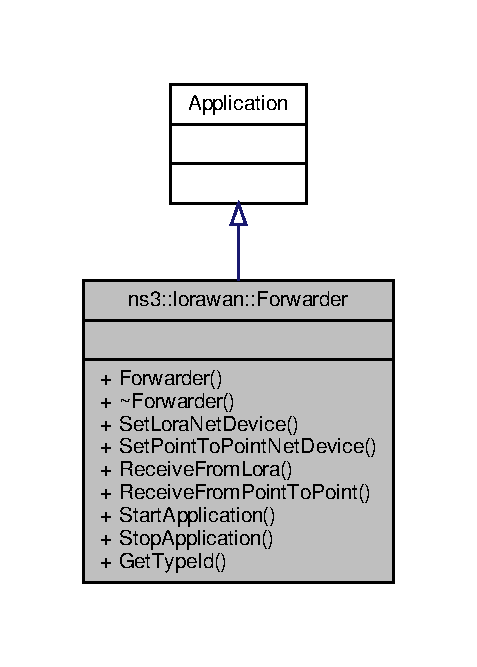
\includegraphics[width=229pt]{classns3_1_1lorawan_1_1Forwarder__inherit__graph}
\end{center}
\end{figure}


Collaboration diagram for ns3\+:\+:lorawan\+:\+:Forwarder\+:
\nopagebreak
\begin{figure}[H]
\begin{center}
\leavevmode
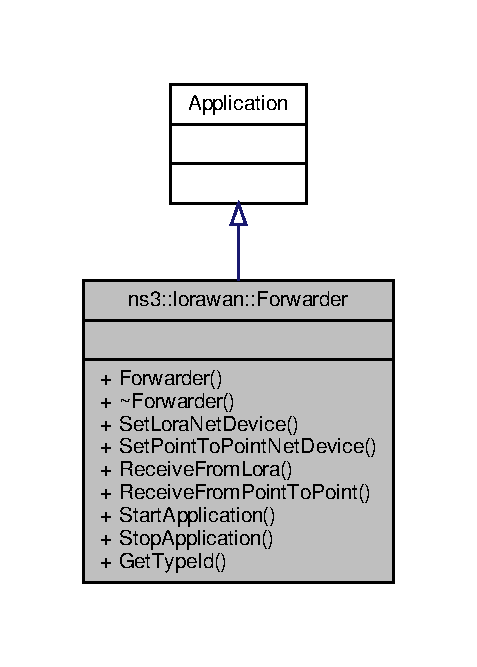
\includegraphics[width=229pt]{classns3_1_1lorawan_1_1Forwarder__coll__graph}
\end{center}
\end{figure}
\subsection*{Public Member Functions}
\begin{DoxyCompactItemize}
\item 
void \hyperlink{classns3_1_1lorawan_1_1Forwarder_ac945060ea56bc2bd25d2b4ff18d80a2d}{Set\+Lora\+Net\+Device} (Ptr$<$ \hyperlink{classns3_1_1lorawan_1_1LoraNetDevice}{Lora\+Net\+Device} $>$ lora\+Net\+Device)
\item 
void \hyperlink{classns3_1_1lorawan_1_1Forwarder_a05e97fcfcdeafe425477f6e0c06509f8}{Set\+Point\+To\+Point\+Net\+Device} (Ptr$<$ Point\+To\+Point\+Net\+Device $>$ point\+To\+Point\+Net\+Device)
\item 
bool \hyperlink{classns3_1_1lorawan_1_1Forwarder_a92407f3228e9cf5b1b84cc7d62dff2c2}{Receive\+From\+Lora} (Ptr$<$ \hyperlink{classNetDevice}{Net\+Device} $>$ lora\+Net\+Device, Ptr$<$ const Packet $>$ packet, uint16\+\_\+t protocol, const Address \&sender)
\item 
bool \hyperlink{classns3_1_1lorawan_1_1Forwarder_a004f5126baf8e3a264cab68f59921f77}{Receive\+From\+Point\+To\+Point} (Ptr$<$ \hyperlink{classNetDevice}{Net\+Device} $>$ point\+To\+Point\+Net\+Device, Ptr$<$ const Packet $>$ packet, uint16\+\_\+t protocol, const Address \&sender)
\item 
void \hyperlink{classns3_1_1lorawan_1_1Forwarder_ae94ef5057f8c5fb01db2c6c7ed17eb9d}{Start\+Application} (void)
\item 
void \hyperlink{classns3_1_1lorawan_1_1Forwarder_a8980a4b970c9b20e3ef27d2ab6d3d1d9}{Stop\+Application} (void)
\end{DoxyCompactItemize}
\subsection*{Static Public Member Functions}
\begin{DoxyCompactItemize}
\item 
\mbox{\Hypertarget{classns3_1_1lorawan_1_1Forwarder_abb352183dd8738c5aab43be37199295b}\label{classns3_1_1lorawan_1_1Forwarder_abb352183dd8738c5aab43be37199295b}} 
static Type\+Id {\bfseries Get\+Type\+Id} (void)
\end{DoxyCompactItemize}


\subsection{Detailed Description}
This application forwards packets between Net\+Devices\+: \hyperlink{classns3_1_1lorawan_1_1LoraNetDevice}{Lora\+Net\+Device} -\/$>$ Point\+To\+Point\+Net\+Device and vice versa. 

\subsection{Member Function Documentation}
\mbox{\Hypertarget{classns3_1_1lorawan_1_1Forwarder_a92407f3228e9cf5b1b84cc7d62dff2c2}\label{classns3_1_1lorawan_1_1Forwarder_a92407f3228e9cf5b1b84cc7d62dff2c2}} 
\index{ns3\+::lorawan\+::\+Forwarder@{ns3\+::lorawan\+::\+Forwarder}!Receive\+From\+Lora@{Receive\+From\+Lora}}
\index{Receive\+From\+Lora@{Receive\+From\+Lora}!ns3\+::lorawan\+::\+Forwarder@{ns3\+::lorawan\+::\+Forwarder}}
\subsubsection{\texorpdfstring{Receive\+From\+Lora()}{ReceiveFromLora()}}
{\footnotesize\ttfamily bool ns3\+::lorawan\+::\+Forwarder\+::\+Receive\+From\+Lora (\begin{DoxyParamCaption}\item[{Ptr$<$ \hyperlink{classNetDevice}{Net\+Device} $>$}]{lora\+Net\+Device,  }\item[{Ptr$<$ const Packet $>$}]{packet,  }\item[{uint16\+\_\+t}]{protocol,  }\item[{const Address \&}]{sender }\end{DoxyParamCaption})}

Receive a packet from the \hyperlink{classns3_1_1lorawan_1_1LoraNetDevice}{Lora\+Net\+Device}.


\begin{DoxyParams}{Parameters}
{\em lora\+Net\+Device} & The \hyperlink{classns3_1_1lorawan_1_1LoraNetDevice}{Lora\+Net\+Device} we received the packet from. \\
\hline
{\em packet} & The packet we received. \\
\hline
{\em protocol} & The protocol number associated to this packet. \\
\hline
{\em sender} & The address of the sender. \\
\hline
\end{DoxyParams}
\begin{DoxyReturn}{Returns}
True if we can handle the packet, false otherwise. 
\end{DoxyReturn}
\mbox{\Hypertarget{classns3_1_1lorawan_1_1Forwarder_a004f5126baf8e3a264cab68f59921f77}\label{classns3_1_1lorawan_1_1Forwarder_a004f5126baf8e3a264cab68f59921f77}} 
\index{ns3\+::lorawan\+::\+Forwarder@{ns3\+::lorawan\+::\+Forwarder}!Receive\+From\+Point\+To\+Point@{Receive\+From\+Point\+To\+Point}}
\index{Receive\+From\+Point\+To\+Point@{Receive\+From\+Point\+To\+Point}!ns3\+::lorawan\+::\+Forwarder@{ns3\+::lorawan\+::\+Forwarder}}
\subsubsection{\texorpdfstring{Receive\+From\+Point\+To\+Point()}{ReceiveFromPointToPoint()}}
{\footnotesize\ttfamily bool ns3\+::lorawan\+::\+Forwarder\+::\+Receive\+From\+Point\+To\+Point (\begin{DoxyParamCaption}\item[{Ptr$<$ \hyperlink{classNetDevice}{Net\+Device} $>$}]{point\+To\+Point\+Net\+Device,  }\item[{Ptr$<$ const Packet $>$}]{packet,  }\item[{uint16\+\_\+t}]{protocol,  }\item[{const Address \&}]{sender }\end{DoxyParamCaption})}

Receive a packet from the Point\+To\+Point\+Net\+Device \mbox{\Hypertarget{classns3_1_1lorawan_1_1Forwarder_ac945060ea56bc2bd25d2b4ff18d80a2d}\label{classns3_1_1lorawan_1_1Forwarder_ac945060ea56bc2bd25d2b4ff18d80a2d}} 
\index{ns3\+::lorawan\+::\+Forwarder@{ns3\+::lorawan\+::\+Forwarder}!Set\+Lora\+Net\+Device@{Set\+Lora\+Net\+Device}}
\index{Set\+Lora\+Net\+Device@{Set\+Lora\+Net\+Device}!ns3\+::lorawan\+::\+Forwarder@{ns3\+::lorawan\+::\+Forwarder}}
\subsubsection{\texorpdfstring{Set\+Lora\+Net\+Device()}{SetLoraNetDevice()}}
{\footnotesize\ttfamily void ns3\+::lorawan\+::\+Forwarder\+::\+Set\+Lora\+Net\+Device (\begin{DoxyParamCaption}\item[{Ptr$<$ \hyperlink{classns3_1_1lorawan_1_1LoraNetDevice}{Lora\+Net\+Device} $>$}]{lora\+Net\+Device }\end{DoxyParamCaption})}

Sets the device to use to communicate with the E\+Ds.


\begin{DoxyParams}{Parameters}
{\em lora\+Net\+Device} & The \hyperlink{classns3_1_1lorawan_1_1LoraNetDevice}{Lora\+Net\+Device} on this node. \\
\hline
\end{DoxyParams}
\mbox{\Hypertarget{classns3_1_1lorawan_1_1Forwarder_a05e97fcfcdeafe425477f6e0c06509f8}\label{classns3_1_1lorawan_1_1Forwarder_a05e97fcfcdeafe425477f6e0c06509f8}} 
\index{ns3\+::lorawan\+::\+Forwarder@{ns3\+::lorawan\+::\+Forwarder}!Set\+Point\+To\+Point\+Net\+Device@{Set\+Point\+To\+Point\+Net\+Device}}
\index{Set\+Point\+To\+Point\+Net\+Device@{Set\+Point\+To\+Point\+Net\+Device}!ns3\+::lorawan\+::\+Forwarder@{ns3\+::lorawan\+::\+Forwarder}}
\subsubsection{\texorpdfstring{Set\+Point\+To\+Point\+Net\+Device()}{SetPointToPointNetDevice()}}
{\footnotesize\ttfamily void ns3\+::lorawan\+::\+Forwarder\+::\+Set\+Point\+To\+Point\+Net\+Device (\begin{DoxyParamCaption}\item[{Ptr$<$ Point\+To\+Point\+Net\+Device $>$}]{point\+To\+Point\+Net\+Device }\end{DoxyParamCaption})}

Sets the P2P device to use to communicate with the NS.


\begin{DoxyParams}{Parameters}
{\em point\+To\+Point\+Net\+Device} & The P2\+P\+Net\+Device on this node. \\
\hline
\end{DoxyParams}
\mbox{\Hypertarget{classns3_1_1lorawan_1_1Forwarder_ae94ef5057f8c5fb01db2c6c7ed17eb9d}\label{classns3_1_1lorawan_1_1Forwarder_ae94ef5057f8c5fb01db2c6c7ed17eb9d}} 
\index{ns3\+::lorawan\+::\+Forwarder@{ns3\+::lorawan\+::\+Forwarder}!Start\+Application@{Start\+Application}}
\index{Start\+Application@{Start\+Application}!ns3\+::lorawan\+::\+Forwarder@{ns3\+::lorawan\+::\+Forwarder}}
\subsubsection{\texorpdfstring{Start\+Application()}{StartApplication()}}
{\footnotesize\ttfamily void ns3\+::lorawan\+::\+Forwarder\+::\+Start\+Application (\begin{DoxyParamCaption}\item[{void}]{ }\end{DoxyParamCaption})}

Start the application \mbox{\Hypertarget{classns3_1_1lorawan_1_1Forwarder_a8980a4b970c9b20e3ef27d2ab6d3d1d9}\label{classns3_1_1lorawan_1_1Forwarder_a8980a4b970c9b20e3ef27d2ab6d3d1d9}} 
\index{ns3\+::lorawan\+::\+Forwarder@{ns3\+::lorawan\+::\+Forwarder}!Stop\+Application@{Stop\+Application}}
\index{Stop\+Application@{Stop\+Application}!ns3\+::lorawan\+::\+Forwarder@{ns3\+::lorawan\+::\+Forwarder}}
\subsubsection{\texorpdfstring{Stop\+Application()}{StopApplication()}}
{\footnotesize\ttfamily void ns3\+::lorawan\+::\+Forwarder\+::\+Stop\+Application (\begin{DoxyParamCaption}\item[{void}]{ }\end{DoxyParamCaption})}

Stop the application 

The documentation for this class was generated from the following files\+:\begin{DoxyCompactItemize}
\item 
forwarder.\+h\item 
forwarder.\+cc\end{DoxyCompactItemize}

\hypertarget{classns3_1_1lorawan_1_1GatewayLoraMac}{}\section{ns3\+:\+:lorawan\+:\+:Gateway\+Lora\+Mac Class Reference}
\label{classns3_1_1lorawan_1_1GatewayLoraMac}\index{ns3\+::lorawan\+::\+Gateway\+Lora\+Mac@{ns3\+::lorawan\+::\+Gateway\+Lora\+Mac}}


Inheritance diagram for ns3\+:\+:lorawan\+:\+:Gateway\+Lora\+Mac\+:
\nopagebreak
\begin{figure}[H]
\begin{center}
\leavevmode
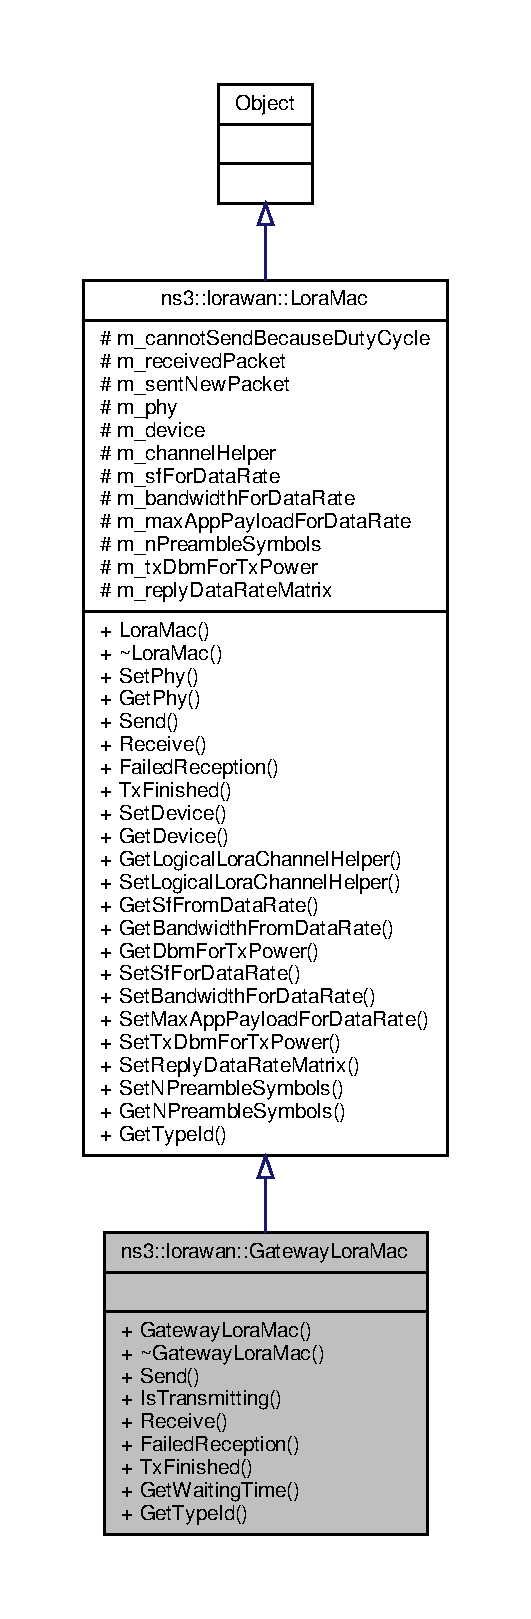
\includegraphics[height=550pt]{classns3_1_1lorawan_1_1GatewayLoraMac__inherit__graph}
\end{center}
\end{figure}


Collaboration diagram for ns3\+:\+:lorawan\+:\+:Gateway\+Lora\+Mac\+:
\nopagebreak
\begin{figure}[H]
\begin{center}
\leavevmode
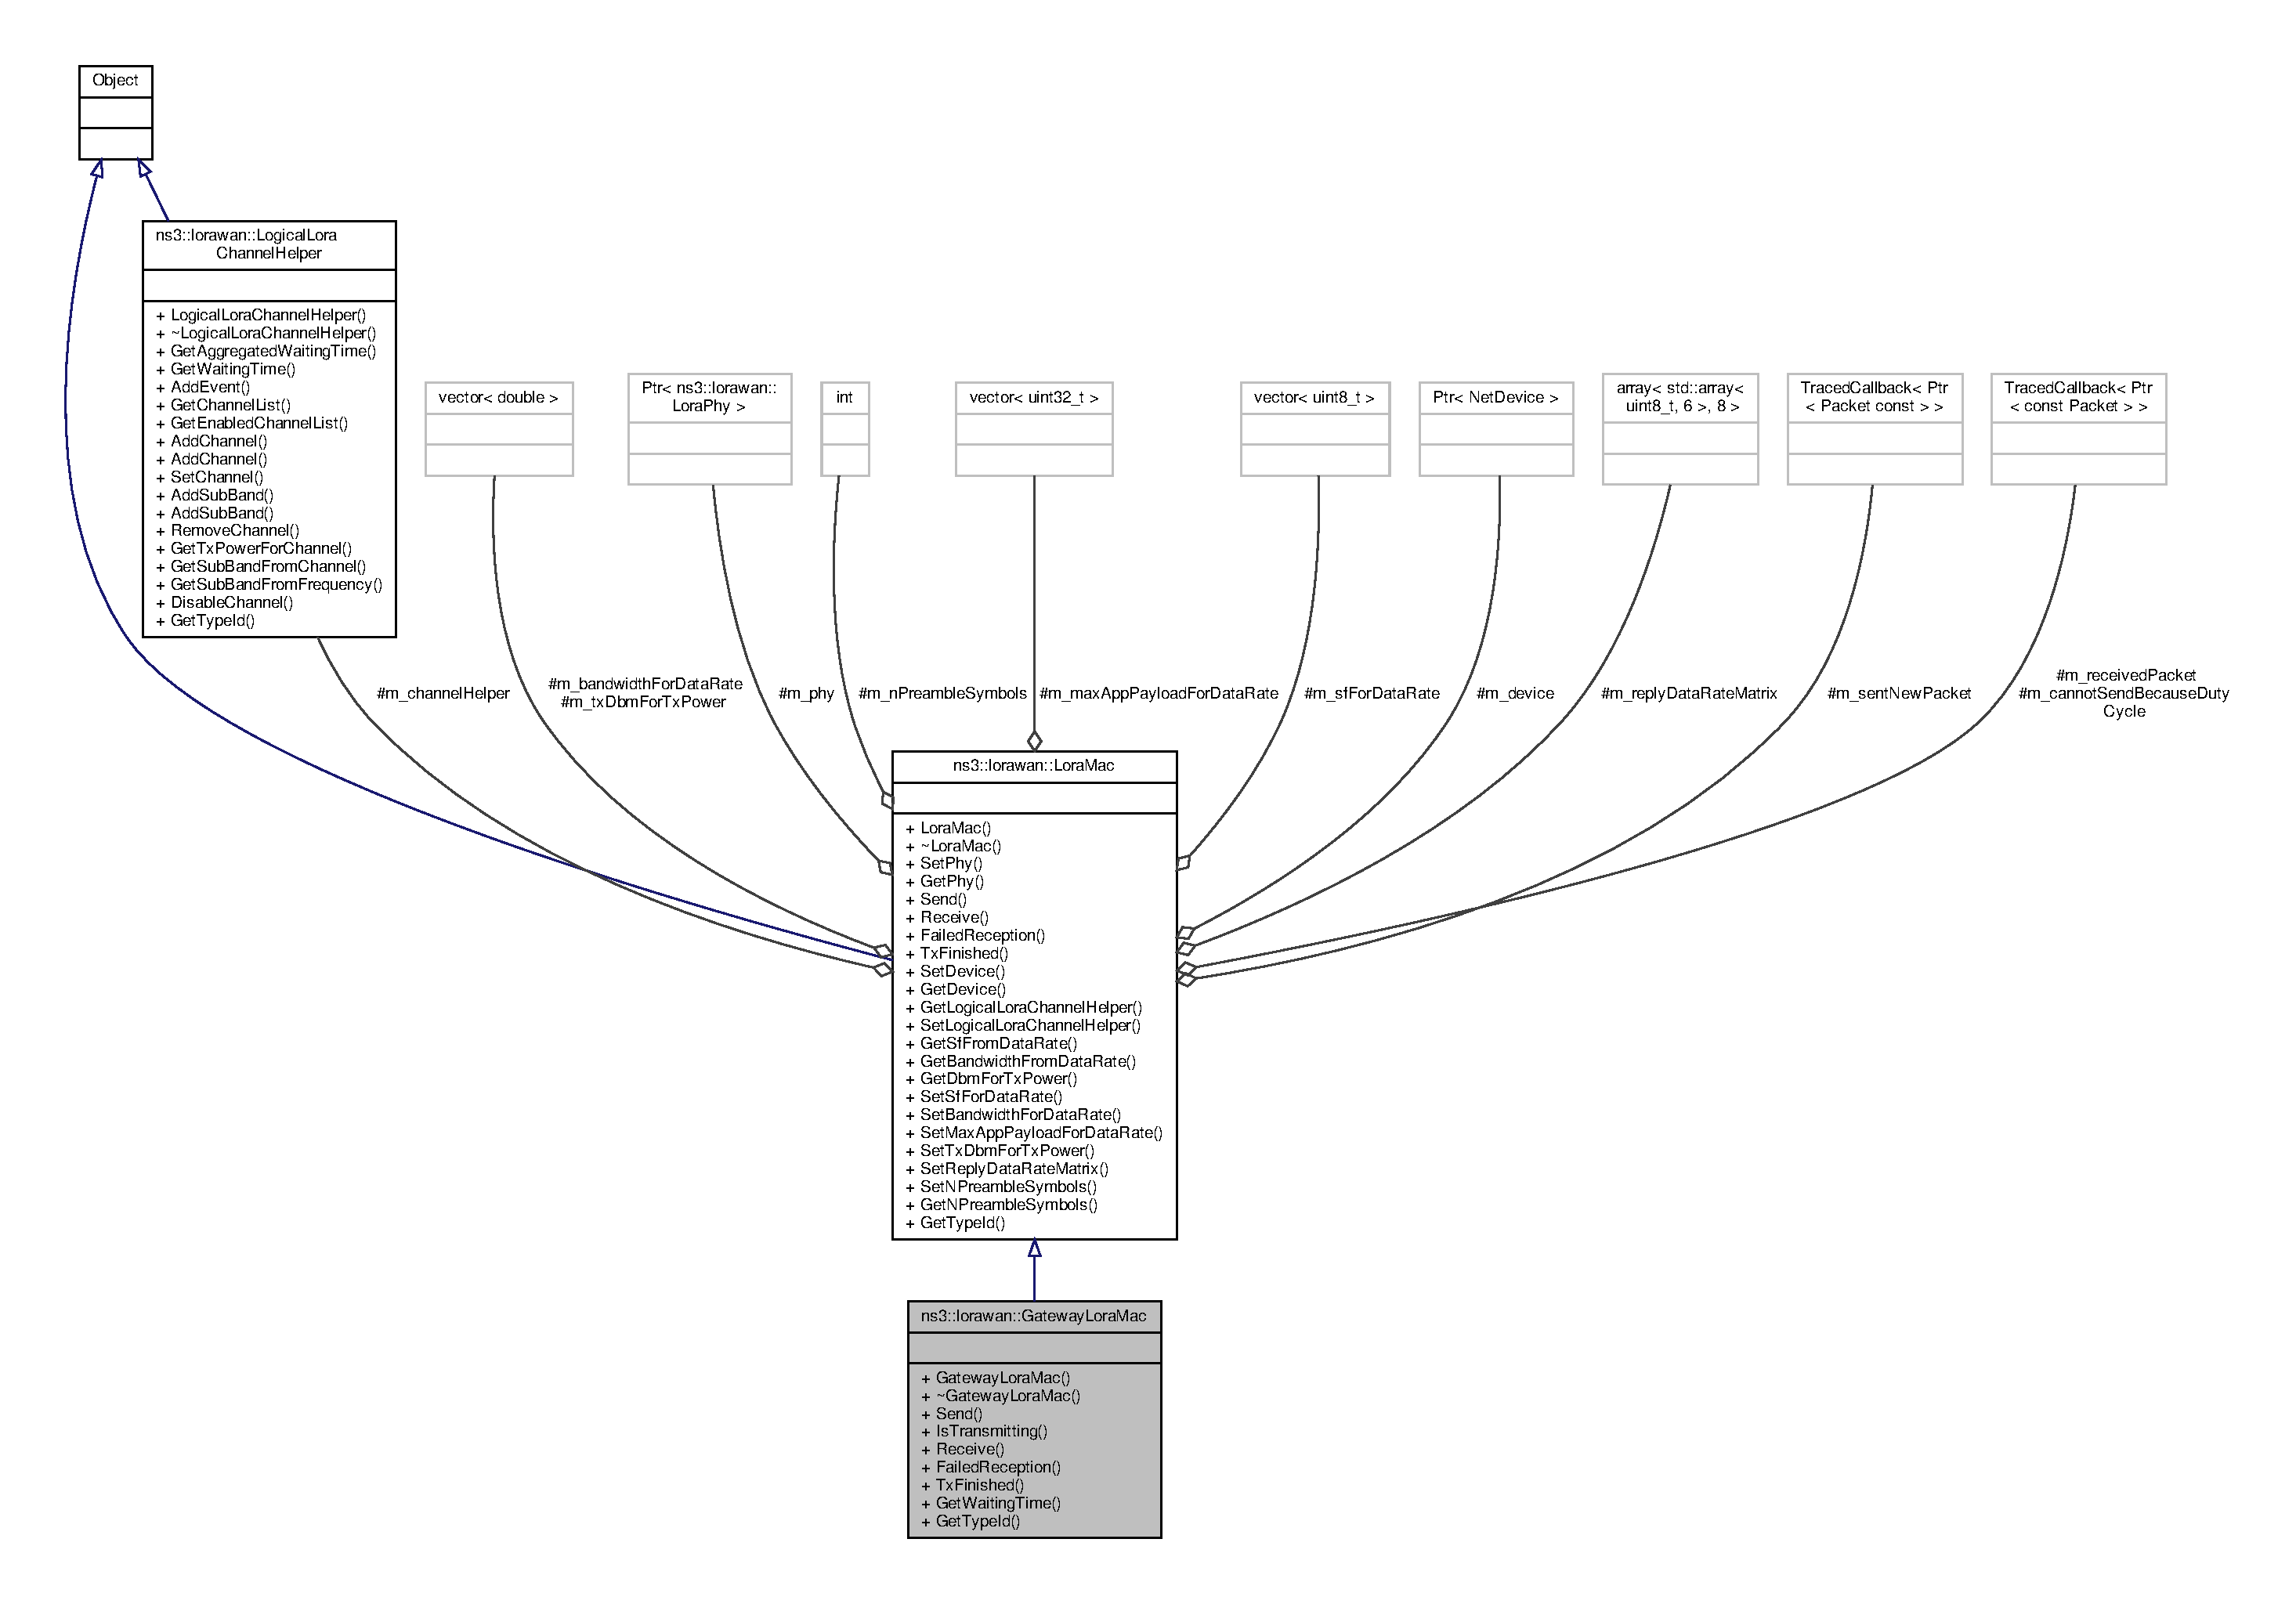
\includegraphics[width=350pt]{classns3_1_1lorawan_1_1GatewayLoraMac__coll__graph}
\end{center}
\end{figure}
\subsection*{Public Member Functions}
\begin{DoxyCompactItemize}
\item 
virtual void \hyperlink{classns3_1_1lorawan_1_1GatewayLoraMac_adc8823176576f9d19d4ae663d88d869e}{Send} (Ptr$<$ Packet $>$ packet)
\item 
\mbox{\Hypertarget{classns3_1_1lorawan_1_1GatewayLoraMac_a2acc1aa214a6bf016e81b7d2fe891173}\label{classns3_1_1lorawan_1_1GatewayLoraMac_a2acc1aa214a6bf016e81b7d2fe891173}} 
bool {\bfseries Is\+Transmitting} (void)
\item 
virtual void \hyperlink{classns3_1_1lorawan_1_1GatewayLoraMac_a8e53a57ec381d76bd47f51581b8c0df7}{Receive} (Ptr$<$ Packet const $>$ packet)
\item 
virtual void \hyperlink{classns3_1_1lorawan_1_1GatewayLoraMac_a2d752f0ff766d409e1eb91d7bcd06ad5}{Failed\+Reception} (Ptr$<$ Packet const $>$ packet)
\item 
virtual void \hyperlink{classns3_1_1lorawan_1_1GatewayLoraMac_a115cbb38716b278b7bac756386a5ae77}{Tx\+Finished} (Ptr$<$ Packet const $>$ packet)
\item 
Time \hyperlink{classns3_1_1lorawan_1_1GatewayLoraMac_ae6271138c9d7b29e588e5b59d67b2c66}{Get\+Waiting\+Time} (double frequency)
\end{DoxyCompactItemize}
\subsection*{Static Public Member Functions}
\begin{DoxyCompactItemize}
\item 
\mbox{\Hypertarget{classns3_1_1lorawan_1_1GatewayLoraMac_a99dcd0d95d3ea8196aa0402d46d98896}\label{classns3_1_1lorawan_1_1GatewayLoraMac_a99dcd0d95d3ea8196aa0402d46d98896}} 
static Type\+Id {\bfseries Get\+Type\+Id} (void)
\end{DoxyCompactItemize}
\subsection*{Additional Inherited Members}


\subsection{Member Function Documentation}
\mbox{\Hypertarget{classns3_1_1lorawan_1_1GatewayLoraMac_a2d752f0ff766d409e1eb91d7bcd06ad5}\label{classns3_1_1lorawan_1_1GatewayLoraMac_a2d752f0ff766d409e1eb91d7bcd06ad5}} 
\index{ns3\+::lorawan\+::\+Gateway\+Lora\+Mac@{ns3\+::lorawan\+::\+Gateway\+Lora\+Mac}!Failed\+Reception@{Failed\+Reception}}
\index{Failed\+Reception@{Failed\+Reception}!ns3\+::lorawan\+::\+Gateway\+Lora\+Mac@{ns3\+::lorawan\+::\+Gateway\+Lora\+Mac}}
\subsubsection{\texorpdfstring{Failed\+Reception()}{FailedReception()}}
{\footnotesize\ttfamily void ns3\+::lorawan\+::\+Gateway\+Lora\+Mac\+::\+Failed\+Reception (\begin{DoxyParamCaption}\item[{Ptr$<$ Packet const $>$}]{packet }\end{DoxyParamCaption})\hspace{0.3cm}{\ttfamily [virtual]}}

Function called by lower layers to inform this layer that reception of a packet we were locked on failed.


\begin{DoxyParams}{Parameters}
{\em packet} & the packet we failed to receive \\
\hline
\end{DoxyParams}


Implements \hyperlink{classns3_1_1lorawan_1_1LoraMac_afcd55472bbfa299c4d0239d5fa9957e3}{ns3\+::lorawan\+::\+Lora\+Mac}.

\mbox{\Hypertarget{classns3_1_1lorawan_1_1GatewayLoraMac_ae6271138c9d7b29e588e5b59d67b2c66}\label{classns3_1_1lorawan_1_1GatewayLoraMac_ae6271138c9d7b29e588e5b59d67b2c66}} 
\index{ns3\+::lorawan\+::\+Gateway\+Lora\+Mac@{ns3\+::lorawan\+::\+Gateway\+Lora\+Mac}!Get\+Waiting\+Time@{Get\+Waiting\+Time}}
\index{Get\+Waiting\+Time@{Get\+Waiting\+Time}!ns3\+::lorawan\+::\+Gateway\+Lora\+Mac@{ns3\+::lorawan\+::\+Gateway\+Lora\+Mac}}
\subsubsection{\texorpdfstring{Get\+Waiting\+Time()}{GetWaitingTime()}}
{\footnotesize\ttfamily Time ns3\+::lorawan\+::\+Gateway\+Lora\+Mac\+::\+Get\+Waiting\+Time (\begin{DoxyParamCaption}\item[{double}]{frequency }\end{DoxyParamCaption})}

Return the next time at which we will be able to transmit.

\begin{DoxyReturn}{Returns}
The next transmission time. 
\end{DoxyReturn}
\mbox{\Hypertarget{classns3_1_1lorawan_1_1GatewayLoraMac_a8e53a57ec381d76bd47f51581b8c0df7}\label{classns3_1_1lorawan_1_1GatewayLoraMac_a8e53a57ec381d76bd47f51581b8c0df7}} 
\index{ns3\+::lorawan\+::\+Gateway\+Lora\+Mac@{ns3\+::lorawan\+::\+Gateway\+Lora\+Mac}!Receive@{Receive}}
\index{Receive@{Receive}!ns3\+::lorawan\+::\+Gateway\+Lora\+Mac@{ns3\+::lorawan\+::\+Gateway\+Lora\+Mac}}
\subsubsection{\texorpdfstring{Receive()}{Receive()}}
{\footnotesize\ttfamily void ns3\+::lorawan\+::\+Gateway\+Lora\+Mac\+::\+Receive (\begin{DoxyParamCaption}\item[{Ptr$<$ Packet const $>$}]{packet }\end{DoxyParamCaption})\hspace{0.3cm}{\ttfamily [virtual]}}

Receive a packet from the lower layer.


\begin{DoxyParams}{Parameters}
{\em packet} & the received packet \\
\hline
\end{DoxyParams}


Implements \hyperlink{classns3_1_1lorawan_1_1LoraMac_a6eda46656789a277b8e103afcefdc21a}{ns3\+::lorawan\+::\+Lora\+Mac}.

\mbox{\Hypertarget{classns3_1_1lorawan_1_1GatewayLoraMac_adc8823176576f9d19d4ae663d88d869e}\label{classns3_1_1lorawan_1_1GatewayLoraMac_adc8823176576f9d19d4ae663d88d869e}} 
\index{ns3\+::lorawan\+::\+Gateway\+Lora\+Mac@{ns3\+::lorawan\+::\+Gateway\+Lora\+Mac}!Send@{Send}}
\index{Send@{Send}!ns3\+::lorawan\+::\+Gateway\+Lora\+Mac@{ns3\+::lorawan\+::\+Gateway\+Lora\+Mac}}
\subsubsection{\texorpdfstring{Send()}{Send()}}
{\footnotesize\ttfamily void ns3\+::lorawan\+::\+Gateway\+Lora\+Mac\+::\+Send (\begin{DoxyParamCaption}\item[{Ptr$<$ Packet $>$}]{packet }\end{DoxyParamCaption})\hspace{0.3cm}{\ttfamily [virtual]}}

Send a packet.


\begin{DoxyParams}{Parameters}
{\em packet} & The packet to send. \\
\hline
\end{DoxyParams}


Implements \hyperlink{classns3_1_1lorawan_1_1LoraMac_ac2f3fd92536658192bfa3d1523fff716}{ns3\+::lorawan\+::\+Lora\+Mac}.

\mbox{\Hypertarget{classns3_1_1lorawan_1_1GatewayLoraMac_a115cbb38716b278b7bac756386a5ae77}\label{classns3_1_1lorawan_1_1GatewayLoraMac_a115cbb38716b278b7bac756386a5ae77}} 
\index{ns3\+::lorawan\+::\+Gateway\+Lora\+Mac@{ns3\+::lorawan\+::\+Gateway\+Lora\+Mac}!Tx\+Finished@{Tx\+Finished}}
\index{Tx\+Finished@{Tx\+Finished}!ns3\+::lorawan\+::\+Gateway\+Lora\+Mac@{ns3\+::lorawan\+::\+Gateway\+Lora\+Mac}}
\subsubsection{\texorpdfstring{Tx\+Finished()}{TxFinished()}}
{\footnotesize\ttfamily void ns3\+::lorawan\+::\+Gateway\+Lora\+Mac\+::\+Tx\+Finished (\begin{DoxyParamCaption}\item[{Ptr$<$ Packet const $>$}]{packet }\end{DoxyParamCaption})\hspace{0.3cm}{\ttfamily [virtual]}}

Perform actions after sending a packet.


\begin{DoxyParams}{Parameters}
{\em packet} & The packet that just finished transmission. \\
\hline
\end{DoxyParams}


Implements \hyperlink{classns3_1_1lorawan_1_1LoraMac_aa64037192af83dc459487bccccd10bdf}{ns3\+::lorawan\+::\+Lora\+Mac}.



The documentation for this class was generated from the following files\+:\begin{DoxyCompactItemize}
\item 
gateway-\/lora-\/mac.\+h\item 
gateway-\/lora-\/mac.\+cc\end{DoxyCompactItemize}

\hypertarget{classns3_1_1lorawan_1_1GatewayLoraPhy}{}\section{ns3\+:\+:lorawan\+:\+:Gateway\+Lora\+Phy Class Reference}
\label{classns3_1_1lorawan_1_1GatewayLoraPhy}\index{ns3\+::lorawan\+::\+Gateway\+Lora\+Phy@{ns3\+::lorawan\+::\+Gateway\+Lora\+Phy}}


{\ttfamily \#include $<$gateway-\/lora-\/phy.\+h$>$}



Inheritance diagram for ns3\+:\+:lorawan\+:\+:Gateway\+Lora\+Phy\+:
\nopagebreak
\begin{figure}[H]
\begin{center}
\leavevmode
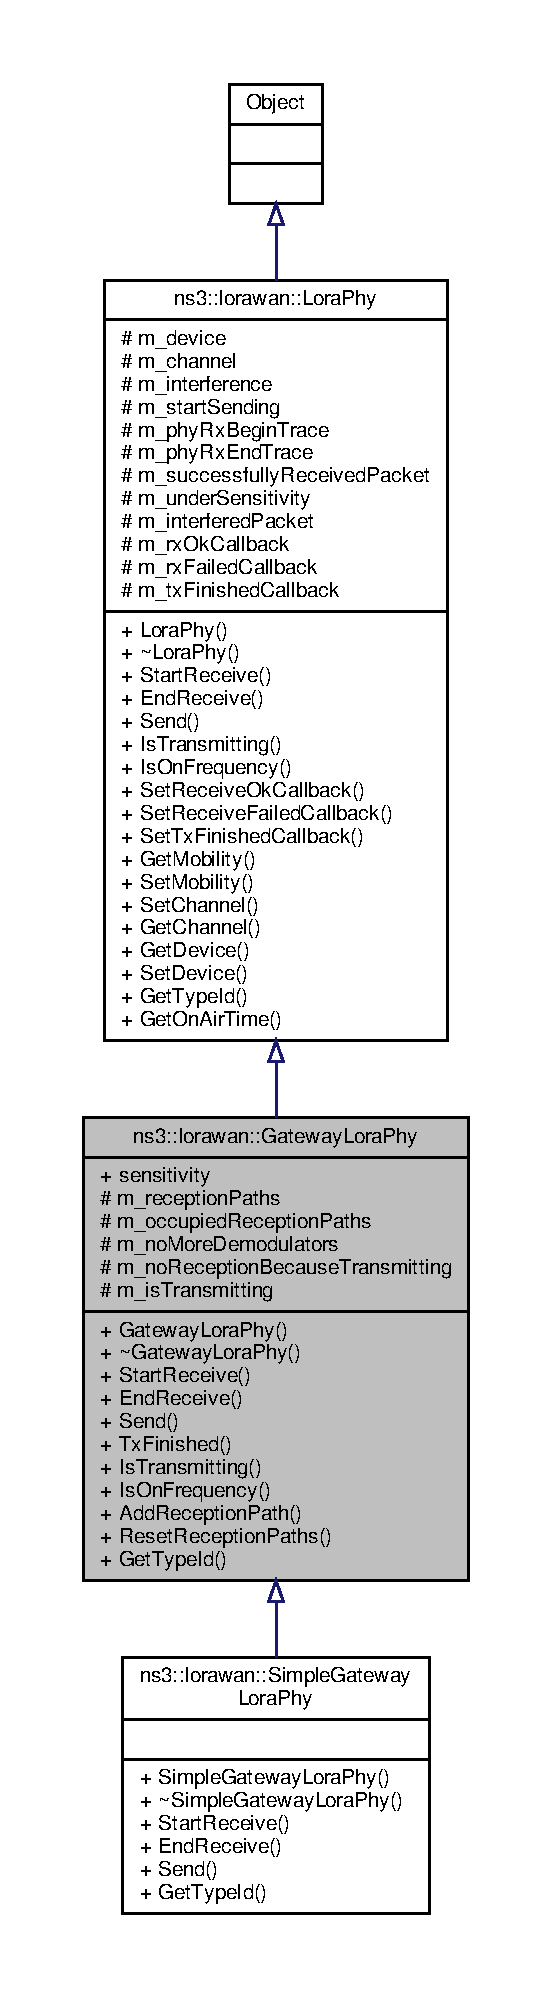
\includegraphics[height=550pt]{classns3_1_1lorawan_1_1GatewayLoraPhy__inherit__graph}
\end{center}
\end{figure}


Collaboration diagram for ns3\+:\+:lorawan\+:\+:Gateway\+Lora\+Phy\+:
\nopagebreak
\begin{figure}[H]
\begin{center}
\leavevmode
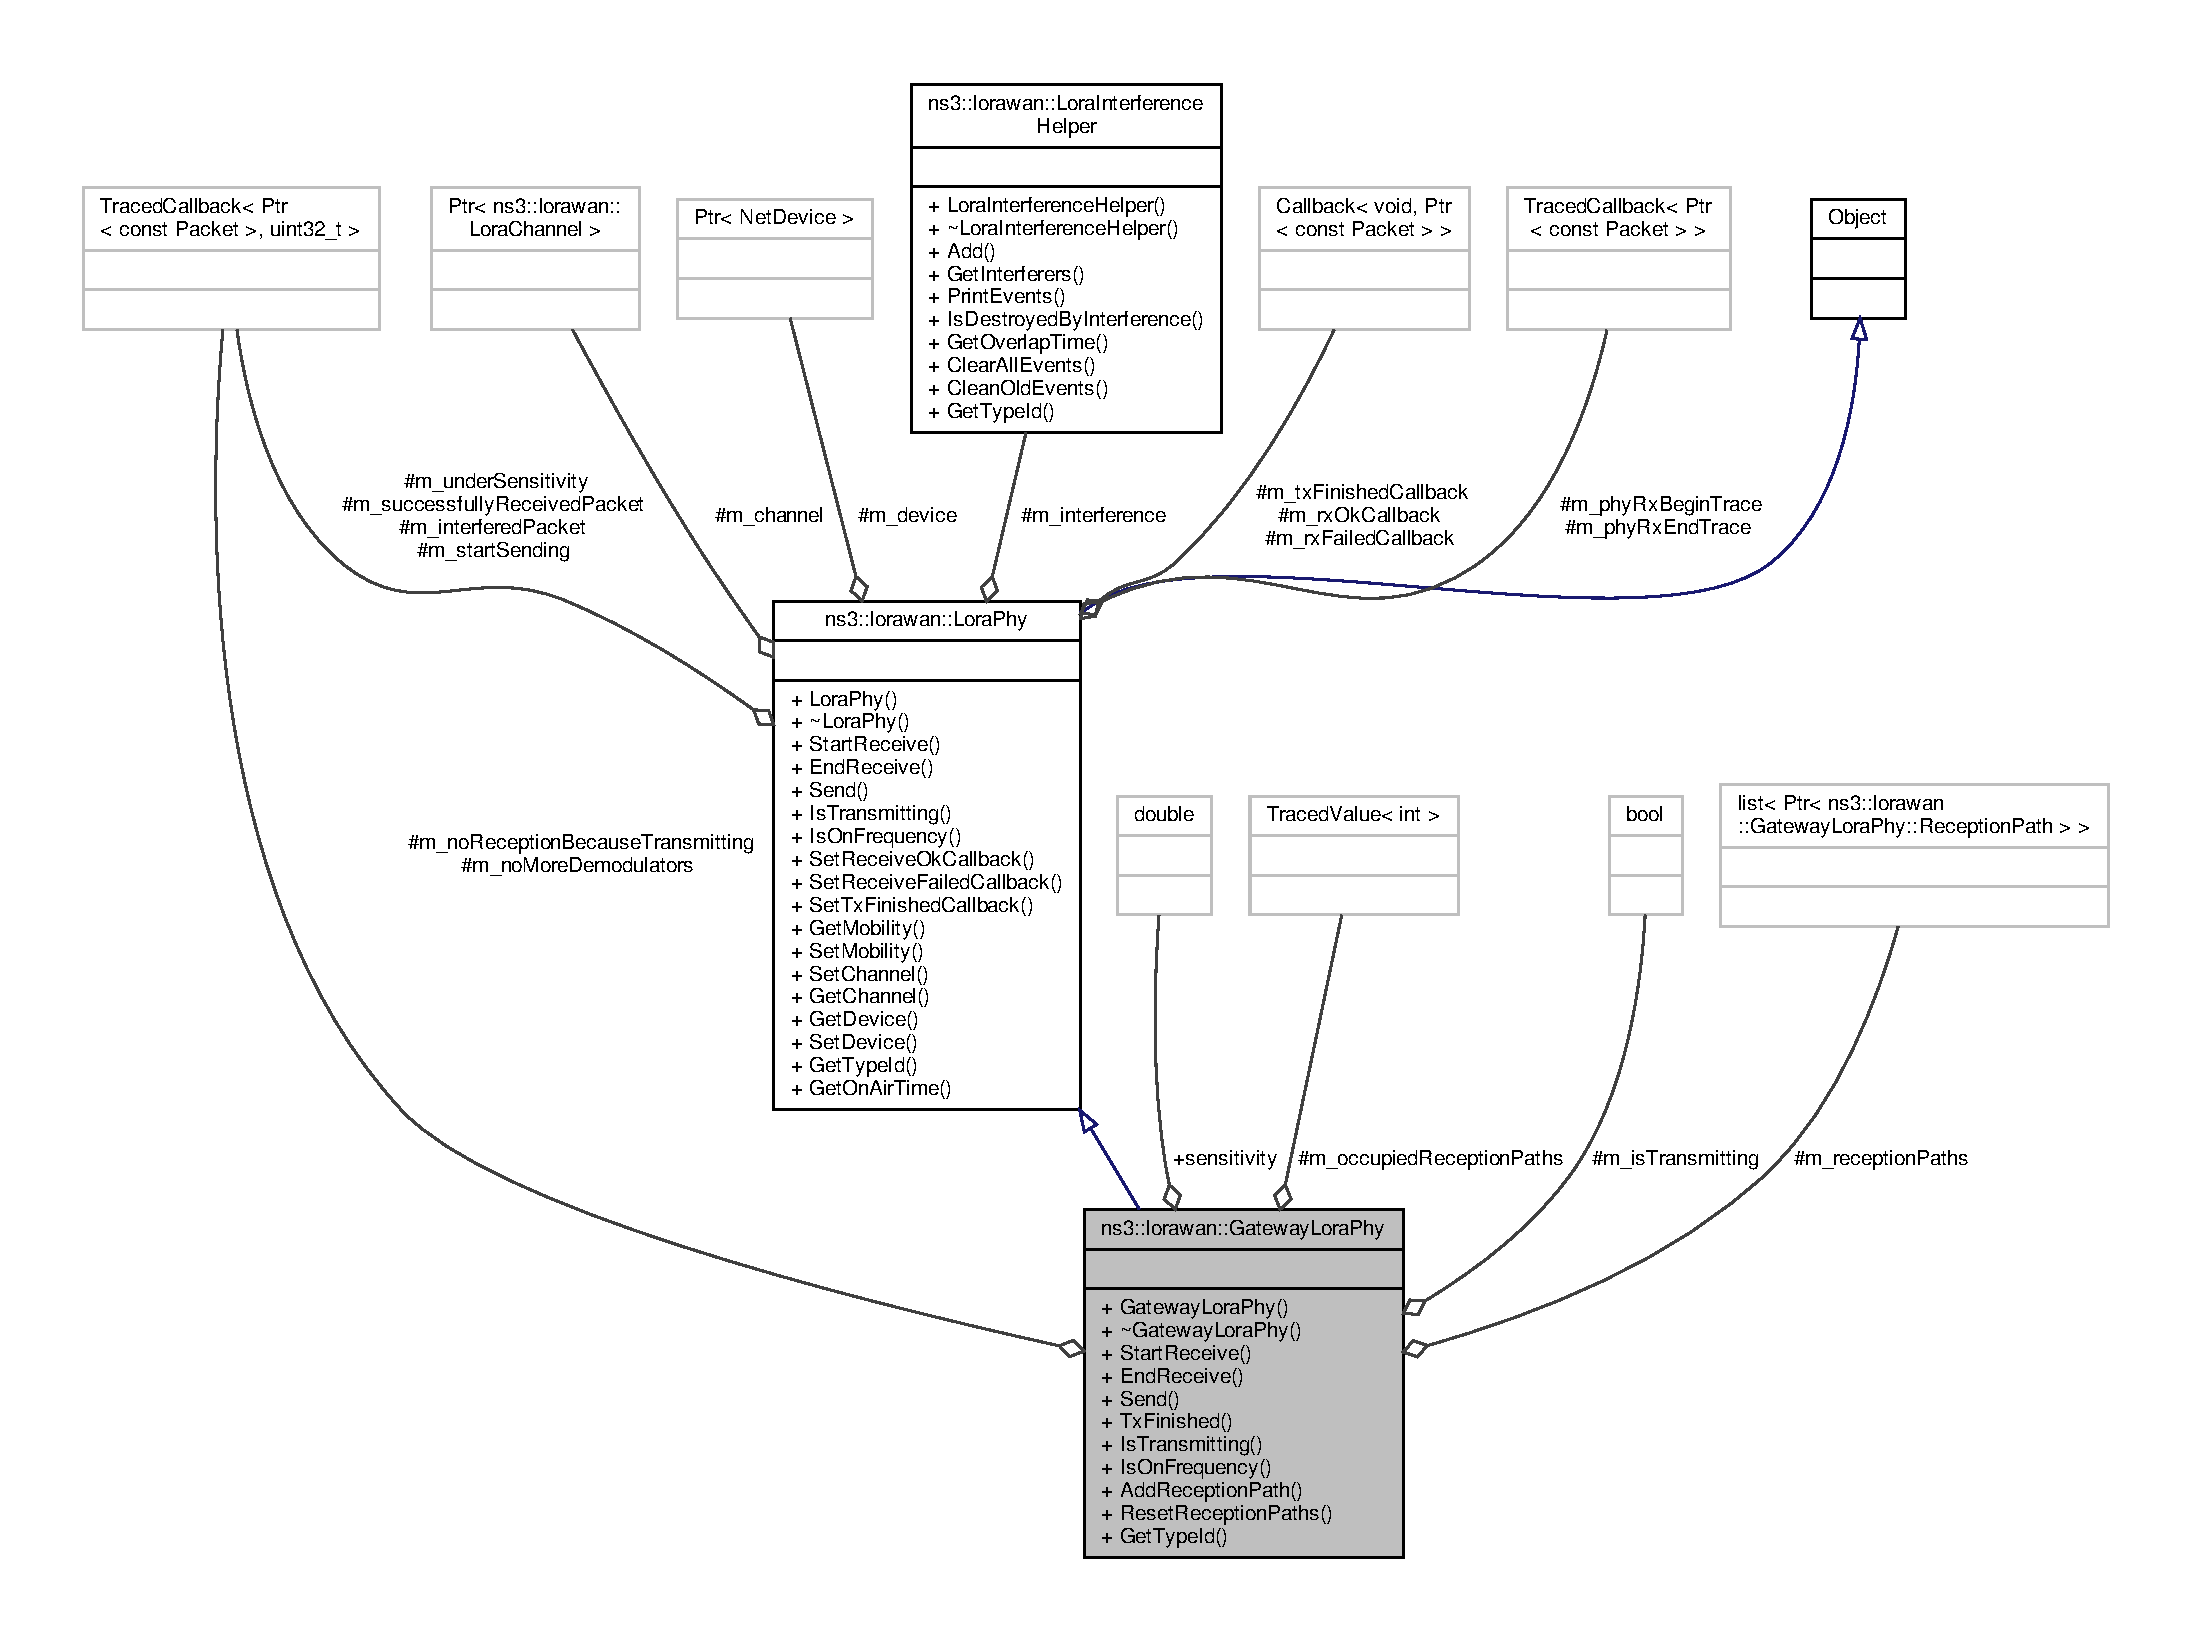
\includegraphics[width=350pt]{classns3_1_1lorawan_1_1GatewayLoraPhy__coll__graph}
\end{center}
\end{figure}
\subsection*{Classes}
\begin{DoxyCompactItemize}
\item 
class \hyperlink{classns3_1_1lorawan_1_1GatewayLoraPhy_1_1ReceptionPath}{Reception\+Path}
\end{DoxyCompactItemize}
\subsection*{Public Member Functions}
\begin{DoxyCompactItemize}
\item 
virtual void \hyperlink{classns3_1_1lorawan_1_1GatewayLoraPhy_a08744b321b5f1b1cf84cff8d7ca8bf49}{Start\+Receive} (Ptr$<$ Packet $>$ packet, double rx\+Power\+Dbm, uint8\+\_\+t sf, Time duration, double frequency\+M\+Hz)=0
\item 
virtual void \hyperlink{classns3_1_1lorawan_1_1GatewayLoraPhy_a030500acf630f508b12923627cdc4068}{End\+Receive} (Ptr$<$ Packet $>$ packet, Ptr$<$ \hyperlink{classns3_1_1lorawan_1_1LoraInterferenceHelper_1_1Event}{Lora\+Interference\+Helper\+::\+Event} $>$ event)=0
\item 
virtual void \hyperlink{classns3_1_1lorawan_1_1GatewayLoraPhy_a2f1375c96d37fd05f1e33e1423826299}{Send} (Ptr$<$ Packet $>$ packet, \hyperlink{structns3_1_1lorawan_1_1LoraTxParameters}{Lora\+Tx\+Parameters} tx\+Params, double frequency\+M\+Hz, double tx\+Power\+Dbm)=0
\item 
\mbox{\Hypertarget{classns3_1_1lorawan_1_1GatewayLoraPhy_a0676e7b725abab9fab81c69ad0c361f5}\label{classns3_1_1lorawan_1_1GatewayLoraPhy_a0676e7b725abab9fab81c69ad0c361f5}} 
virtual void {\bfseries Tx\+Finished} (Ptr$<$ Packet $>$ packet)
\item 
bool \hyperlink{classns3_1_1lorawan_1_1GatewayLoraPhy_a9184985bc4da2d1c0cc9fedb105b20f8}{Is\+Transmitting} (void)
\item 
virtual bool \hyperlink{classns3_1_1lorawan_1_1GatewayLoraPhy_a293b678aaaf872fb1d6c0385bbab9d71}{Is\+On\+Frequency} (double frequency\+M\+Hz)
\item 
void \hyperlink{classns3_1_1lorawan_1_1GatewayLoraPhy_a5587bc3145215aad3faa2b522db5595b}{Add\+Reception\+Path} (double frequency\+M\+Hz)
\item 
void \hyperlink{classns3_1_1lorawan_1_1GatewayLoraPhy_aa964c821ed36fce6815910898ddfbb71}{Reset\+Reception\+Paths} (void)
\end{DoxyCompactItemize}
\subsection*{Static Public Member Functions}
\begin{DoxyCompactItemize}
\item 
\mbox{\Hypertarget{classns3_1_1lorawan_1_1GatewayLoraPhy_ad43bcb346c3b0fba2787817014ee49d5}\label{classns3_1_1lorawan_1_1GatewayLoraPhy_ad43bcb346c3b0fba2787817014ee49d5}} 
static Type\+Id {\bfseries Get\+Type\+Id} (void)
\end{DoxyCompactItemize}
\subsection*{Static Public Attributes}
\begin{DoxyCompactItemize}
\item 
static const double \hyperlink{classns3_1_1lorawan_1_1GatewayLoraPhy_a5e087b8d88cf37e3c81d189876cb3b67}{sensitivity} \mbox{[}6\mbox{]}
\end{DoxyCompactItemize}
\subsection*{Protected Attributes}
\begin{DoxyCompactItemize}
\item 
std\+::list$<$ Ptr$<$ \hyperlink{classns3_1_1lorawan_1_1GatewayLoraPhy_1_1ReceptionPath}{Reception\+Path} $>$ $>$ \hyperlink{classns3_1_1lorawan_1_1GatewayLoraPhy_ad76f73bdb7fe35f39eaf75cf619445fc}{m\+\_\+reception\+Paths}
\item 
Traced\+Value$<$ int $>$ \hyperlink{classns3_1_1lorawan_1_1GatewayLoraPhy_a4cf88e2deb82b7739dd028c6122e1ad4}{m\+\_\+occupied\+Reception\+Paths}
\item 
Traced\+Callback$<$ Ptr$<$ const Packet $>$, uint32\+\_\+t $>$ \hyperlink{classns3_1_1lorawan_1_1GatewayLoraPhy_ae88528e820900ced7285b7993622cdc5}{m\+\_\+no\+More\+Demodulators}
\item 
Traced\+Callback$<$ Ptr$<$ const Packet $>$, uint32\+\_\+t $>$ \hyperlink{classns3_1_1lorawan_1_1GatewayLoraPhy_a69dbd2dafaea10f75115f2eb38ae06dd}{m\+\_\+no\+Reception\+Because\+Transmitting}
\item 
\mbox{\Hypertarget{classns3_1_1lorawan_1_1GatewayLoraPhy_a0eb1bd0116270a374e1ebdf461da7c22}\label{classns3_1_1lorawan_1_1GatewayLoraPhy_a0eb1bd0116270a374e1ebdf461da7c22}} 
bool \hyperlink{classns3_1_1lorawan_1_1GatewayLoraPhy_a0eb1bd0116270a374e1ebdf461da7c22}{m\+\_\+is\+Transmitting}
\begin{DoxyCompactList}\small\item\em Flag indicating whether a transmission is going on. \end{DoxyCompactList}\end{DoxyCompactItemize}
\subsection*{Additional Inherited Members}


\subsection{Detailed Description}
Class modeling a Lora S\+X1301 chip.

This class models the behaviour of the chip employed in Lora gateways. These chips are characterized by the presence of 8 receive paths, or parallel receivers, which can be employed to listen to different channels simultaneously. This characteristic of the chip is modeled using the Receive\+Path class, which describes a single parallel receiver. \hyperlink{classns3_1_1lorawan_1_1GatewayLoraPhy}{Gateway\+Lora\+Phy} essentially holds and manages a collection of these objects. 

\subsection{Member Function Documentation}
\mbox{\Hypertarget{classns3_1_1lorawan_1_1GatewayLoraPhy_a5587bc3145215aad3faa2b522db5595b}\label{classns3_1_1lorawan_1_1GatewayLoraPhy_a5587bc3145215aad3faa2b522db5595b}} 
\index{ns3\+::lorawan\+::\+Gateway\+Lora\+Phy@{ns3\+::lorawan\+::\+Gateway\+Lora\+Phy}!Add\+Reception\+Path@{Add\+Reception\+Path}}
\index{Add\+Reception\+Path@{Add\+Reception\+Path}!ns3\+::lorawan\+::\+Gateway\+Lora\+Phy@{ns3\+::lorawan\+::\+Gateway\+Lora\+Phy}}
\subsubsection{\texorpdfstring{Add\+Reception\+Path()}{AddReceptionPath()}}
{\footnotesize\ttfamily void ns3\+::lorawan\+::\+Gateway\+Lora\+Phy\+::\+Add\+Reception\+Path (\begin{DoxyParamCaption}\item[{double}]{frequency\+M\+Hz }\end{DoxyParamCaption})}

Add a reception path, locked on a specific frequency.


\begin{DoxyParams}{Parameters}
{\em frequency\+M\+Hz} & The frequency on which to set this \hyperlink{classns3_1_1lorawan_1_1GatewayLoraPhy_1_1ReceptionPath}{Reception\+Path}. \\
\hline
\end{DoxyParams}
\mbox{\Hypertarget{classns3_1_1lorawan_1_1GatewayLoraPhy_a030500acf630f508b12923627cdc4068}\label{classns3_1_1lorawan_1_1GatewayLoraPhy_a030500acf630f508b12923627cdc4068}} 
\index{ns3\+::lorawan\+::\+Gateway\+Lora\+Phy@{ns3\+::lorawan\+::\+Gateway\+Lora\+Phy}!End\+Receive@{End\+Receive}}
\index{End\+Receive@{End\+Receive}!ns3\+::lorawan\+::\+Gateway\+Lora\+Phy@{ns3\+::lorawan\+::\+Gateway\+Lora\+Phy}}
\subsubsection{\texorpdfstring{End\+Receive()}{EndReceive()}}
{\footnotesize\ttfamily virtual void ns3\+::lorawan\+::\+Gateway\+Lora\+Phy\+::\+End\+Receive (\begin{DoxyParamCaption}\item[{Ptr$<$ Packet $>$}]{packet,  }\item[{Ptr$<$ \hyperlink{classns3_1_1lorawan_1_1LoraInterferenceHelper_1_1Event}{Lora\+Interference\+Helper\+::\+Event} $>$}]{event }\end{DoxyParamCaption})\hspace{0.3cm}{\ttfamily [pure virtual]}}

Finish reception of a packet.

This method is scheduled by Start\+Receive, based on the packet duration. By passing a \hyperlink{classns3_1_1lorawan_1_1LoraInterferenceHelper}{Lora\+Interference\+Helper} Event to this method, the class will be able to identify the packet that is being received among all those that were registered as interference by Start\+Receive.


\begin{DoxyParams}{Parameters}
{\em packet} & The received packet. \\
\hline
{\em event} & The event that is tied to this packet in the \hyperlink{classns3_1_1lorawan_1_1LoraInterferenceHelper}{Lora\+Interference\+Helper}. \\
\hline
\end{DoxyParams}


Implements \hyperlink{classns3_1_1lorawan_1_1LoraPhy_a719f749890c247abc3fda290d384c37f}{ns3\+::lorawan\+::\+Lora\+Phy}.



Implemented in \hyperlink{classns3_1_1lorawan_1_1SimpleGatewayLoraPhy_aefb2464599926253bfb1003fa14f8fae}{ns3\+::lorawan\+::\+Simple\+Gateway\+Lora\+Phy}.

\mbox{\Hypertarget{classns3_1_1lorawan_1_1GatewayLoraPhy_a293b678aaaf872fb1d6c0385bbab9d71}\label{classns3_1_1lorawan_1_1GatewayLoraPhy_a293b678aaaf872fb1d6c0385bbab9d71}} 
\index{ns3\+::lorawan\+::\+Gateway\+Lora\+Phy@{ns3\+::lorawan\+::\+Gateway\+Lora\+Phy}!Is\+On\+Frequency@{Is\+On\+Frequency}}
\index{Is\+On\+Frequency@{Is\+On\+Frequency}!ns3\+::lorawan\+::\+Gateway\+Lora\+Phy@{ns3\+::lorawan\+::\+Gateway\+Lora\+Phy}}
\subsubsection{\texorpdfstring{Is\+On\+Frequency()}{IsOnFrequency()}}
{\footnotesize\ttfamily bool ns3\+::lorawan\+::\+Gateway\+Lora\+Phy\+::\+Is\+On\+Frequency (\begin{DoxyParamCaption}\item[{double}]{frequency }\end{DoxyParamCaption})\hspace{0.3cm}{\ttfamily [virtual]}}

Whether this device is listening on the specified frequency or not.


\begin{DoxyParams}{Parameters}
{\em frequency} & The frequency to query. \\
\hline
\end{DoxyParams}
\begin{DoxyReturn}{Returns}
true if the device is listening on that frequency, false otherwise. 
\end{DoxyReturn}


Implements \hyperlink{classns3_1_1lorawan_1_1LoraPhy_a554597e30a17b099e8a7f68242cb16a7}{ns3\+::lorawan\+::\+Lora\+Phy}.

\mbox{\Hypertarget{classns3_1_1lorawan_1_1GatewayLoraPhy_a9184985bc4da2d1c0cc9fedb105b20f8}\label{classns3_1_1lorawan_1_1GatewayLoraPhy_a9184985bc4da2d1c0cc9fedb105b20f8}} 
\index{ns3\+::lorawan\+::\+Gateway\+Lora\+Phy@{ns3\+::lorawan\+::\+Gateway\+Lora\+Phy}!Is\+Transmitting@{Is\+Transmitting}}
\index{Is\+Transmitting@{Is\+Transmitting}!ns3\+::lorawan\+::\+Gateway\+Lora\+Phy@{ns3\+::lorawan\+::\+Gateway\+Lora\+Phy}}
\subsubsection{\texorpdfstring{Is\+Transmitting()}{IsTransmitting()}}
{\footnotesize\ttfamily bool ns3\+::lorawan\+::\+Gateway\+Lora\+Phy\+::\+Is\+Transmitting (\begin{DoxyParamCaption}\item[{void}]{ }\end{DoxyParamCaption})\hspace{0.3cm}{\ttfamily [virtual]}}

Whether this device is transmitting or not.

\begin{DoxyReturn}{Returns}
true if the device is currently transmitting a packet, false otherwise. 
\end{DoxyReturn}


Implements \hyperlink{classns3_1_1lorawan_1_1LoraPhy_a5280764d934ba5ff8d305b0bc6b600ce}{ns3\+::lorawan\+::\+Lora\+Phy}.

\mbox{\Hypertarget{classns3_1_1lorawan_1_1GatewayLoraPhy_aa964c821ed36fce6815910898ddfbb71}\label{classns3_1_1lorawan_1_1GatewayLoraPhy_aa964c821ed36fce6815910898ddfbb71}} 
\index{ns3\+::lorawan\+::\+Gateway\+Lora\+Phy@{ns3\+::lorawan\+::\+Gateway\+Lora\+Phy}!Reset\+Reception\+Paths@{Reset\+Reception\+Paths}}
\index{Reset\+Reception\+Paths@{Reset\+Reception\+Paths}!ns3\+::lorawan\+::\+Gateway\+Lora\+Phy@{ns3\+::lorawan\+::\+Gateway\+Lora\+Phy}}
\subsubsection{\texorpdfstring{Reset\+Reception\+Paths()}{ResetReceptionPaths()}}
{\footnotesize\ttfamily void ns3\+::lorawan\+::\+Gateway\+Lora\+Phy\+::\+Reset\+Reception\+Paths (\begin{DoxyParamCaption}\item[{void}]{ }\end{DoxyParamCaption})}

Reset the list of reception paths.

This method deletes all currently available \hyperlink{classns3_1_1lorawan_1_1GatewayLoraPhy_1_1ReceptionPath}{Reception\+Path} objects. \mbox{\Hypertarget{classns3_1_1lorawan_1_1GatewayLoraPhy_a2f1375c96d37fd05f1e33e1423826299}\label{classns3_1_1lorawan_1_1GatewayLoraPhy_a2f1375c96d37fd05f1e33e1423826299}} 
\index{ns3\+::lorawan\+::\+Gateway\+Lora\+Phy@{ns3\+::lorawan\+::\+Gateway\+Lora\+Phy}!Send@{Send}}
\index{Send@{Send}!ns3\+::lorawan\+::\+Gateway\+Lora\+Phy@{ns3\+::lorawan\+::\+Gateway\+Lora\+Phy}}
\subsubsection{\texorpdfstring{Send()}{Send()}}
{\footnotesize\ttfamily virtual void ns3\+::lorawan\+::\+Gateway\+Lora\+Phy\+::\+Send (\begin{DoxyParamCaption}\item[{Ptr$<$ Packet $>$}]{packet,  }\item[{\hyperlink{structns3_1_1lorawan_1_1LoraTxParameters}{Lora\+Tx\+Parameters}}]{tx\+Params,  }\item[{double}]{frequency\+M\+Hz,  }\item[{double}]{tx\+Power\+Dbm }\end{DoxyParamCaption})\hspace{0.3cm}{\ttfamily [pure virtual]}}

Instruct the P\+HY to send a packet according to some parameters.


\begin{DoxyParams}{Parameters}
{\em packet} & The packet to send. \\
\hline
{\em tx\+Params} & The desired transmission parameters. \\
\hline
{\em frequency\+M\+Hz} & The frequency on which to transmit. \\
\hline
{\em tx\+Power\+Dbm} & The power in d\+Bm with which to transmit the packet. \\
\hline
\end{DoxyParams}


Implements \hyperlink{classns3_1_1lorawan_1_1LoraPhy_a2b940beff4a2fbfb2e603d5d9e65d863}{ns3\+::lorawan\+::\+Lora\+Phy}.



Implemented in \hyperlink{classns3_1_1lorawan_1_1SimpleGatewayLoraPhy_ab65ad475c7a03520d6e03bdd008b8d93}{ns3\+::lorawan\+::\+Simple\+Gateway\+Lora\+Phy}.

\mbox{\Hypertarget{classns3_1_1lorawan_1_1GatewayLoraPhy_a08744b321b5f1b1cf84cff8d7ca8bf49}\label{classns3_1_1lorawan_1_1GatewayLoraPhy_a08744b321b5f1b1cf84cff8d7ca8bf49}} 
\index{ns3\+::lorawan\+::\+Gateway\+Lora\+Phy@{ns3\+::lorawan\+::\+Gateway\+Lora\+Phy}!Start\+Receive@{Start\+Receive}}
\index{Start\+Receive@{Start\+Receive}!ns3\+::lorawan\+::\+Gateway\+Lora\+Phy@{ns3\+::lorawan\+::\+Gateway\+Lora\+Phy}}
\subsubsection{\texorpdfstring{Start\+Receive()}{StartReceive()}}
{\footnotesize\ttfamily virtual void ns3\+::lorawan\+::\+Gateway\+Lora\+Phy\+::\+Start\+Receive (\begin{DoxyParamCaption}\item[{Ptr$<$ Packet $>$}]{packet,  }\item[{double}]{rx\+Power\+Dbm,  }\item[{uint8\+\_\+t}]{sf,  }\item[{Time}]{duration,  }\item[{double}]{frequency\+M\+Hz }\end{DoxyParamCaption})\hspace{0.3cm}{\ttfamily [pure virtual]}}

Start receiving a packet.

This method is typically called by \hyperlink{classns3_1_1lorawan_1_1LoraChannel}{Lora\+Channel}.


\begin{DoxyParams}{Parameters}
{\em packet} & The packet that is arriving at this P\+HY layer. \\
\hline
{\em rx\+Power\+Dbm} & The power of the arriving packet (assumed to be constant for the whole reception). \\
\hline
{\em sf} & The Spreading Factor of the arriving packet. \\
\hline
{\em duration} & The on air time of this packet. \\
\hline
{\em frequency\+M\+Hz} & The frequency this packet is being transmitted on. \\
\hline
\end{DoxyParams}


Implements \hyperlink{classns3_1_1lorawan_1_1LoraPhy_aeeccb517d12084e12e36b533db22386b}{ns3\+::lorawan\+::\+Lora\+Phy}.



Implemented in \hyperlink{classns3_1_1lorawan_1_1SimpleGatewayLoraPhy_a8ed607e9a11e4c0b759d456a35b68c40}{ns3\+::lorawan\+::\+Simple\+Gateway\+Lora\+Phy}.



\subsection{Member Data Documentation}
\mbox{\Hypertarget{classns3_1_1lorawan_1_1GatewayLoraPhy_ae88528e820900ced7285b7993622cdc5}\label{classns3_1_1lorawan_1_1GatewayLoraPhy_ae88528e820900ced7285b7993622cdc5}} 
\index{ns3\+::lorawan\+::\+Gateway\+Lora\+Phy@{ns3\+::lorawan\+::\+Gateway\+Lora\+Phy}!m\+\_\+no\+More\+Demodulators@{m\+\_\+no\+More\+Demodulators}}
\index{m\+\_\+no\+More\+Demodulators@{m\+\_\+no\+More\+Demodulators}!ns3\+::lorawan\+::\+Gateway\+Lora\+Phy@{ns3\+::lorawan\+::\+Gateway\+Lora\+Phy}}
\subsubsection{\texorpdfstring{m\+\_\+no\+More\+Demodulators}{m\_noMoreDemodulators}}
{\footnotesize\ttfamily Traced\+Callback$<$Ptr$<$const Packet$>$, uint32\+\_\+t$>$ ns3\+::lorawan\+::\+Gateway\+Lora\+Phy\+::m\+\_\+no\+More\+Demodulators\hspace{0.3cm}{\ttfamily [protected]}}

Trace source that is fired when a packet cannot be received because all available Receive\+Path instances are busy.

\begin{DoxySeeAlso}{See also}
class Call\+Back\+Trace\+Source 
\end{DoxySeeAlso}
\mbox{\Hypertarget{classns3_1_1lorawan_1_1GatewayLoraPhy_a69dbd2dafaea10f75115f2eb38ae06dd}\label{classns3_1_1lorawan_1_1GatewayLoraPhy_a69dbd2dafaea10f75115f2eb38ae06dd}} 
\index{ns3\+::lorawan\+::\+Gateway\+Lora\+Phy@{ns3\+::lorawan\+::\+Gateway\+Lora\+Phy}!m\+\_\+no\+Reception\+Because\+Transmitting@{m\+\_\+no\+Reception\+Because\+Transmitting}}
\index{m\+\_\+no\+Reception\+Because\+Transmitting@{m\+\_\+no\+Reception\+Because\+Transmitting}!ns3\+::lorawan\+::\+Gateway\+Lora\+Phy@{ns3\+::lorawan\+::\+Gateway\+Lora\+Phy}}
\subsubsection{\texorpdfstring{m\+\_\+no\+Reception\+Because\+Transmitting}{m\_noReceptionBecauseTransmitting}}
{\footnotesize\ttfamily Traced\+Callback$<$Ptr$<$const Packet$>$, uint32\+\_\+t$>$ ns3\+::lorawan\+::\+Gateway\+Lora\+Phy\+::m\+\_\+no\+Reception\+Because\+Transmitting\hspace{0.3cm}{\ttfamily [protected]}}

Trace source that is fired when a packet cannot be received because the Gateway is in transmission state.

\begin{DoxySeeAlso}{See also}
class Call\+Back\+Trace\+Source 
\end{DoxySeeAlso}
\mbox{\Hypertarget{classns3_1_1lorawan_1_1GatewayLoraPhy_a4cf88e2deb82b7739dd028c6122e1ad4}\label{classns3_1_1lorawan_1_1GatewayLoraPhy_a4cf88e2deb82b7739dd028c6122e1ad4}} 
\index{ns3\+::lorawan\+::\+Gateway\+Lora\+Phy@{ns3\+::lorawan\+::\+Gateway\+Lora\+Phy}!m\+\_\+occupied\+Reception\+Paths@{m\+\_\+occupied\+Reception\+Paths}}
\index{m\+\_\+occupied\+Reception\+Paths@{m\+\_\+occupied\+Reception\+Paths}!ns3\+::lorawan\+::\+Gateway\+Lora\+Phy@{ns3\+::lorawan\+::\+Gateway\+Lora\+Phy}}
\subsubsection{\texorpdfstring{m\+\_\+occupied\+Reception\+Paths}{m\_occupiedReceptionPaths}}
{\footnotesize\ttfamily Traced\+Value$<$int$>$ ns3\+::lorawan\+::\+Gateway\+Lora\+Phy\+::m\+\_\+occupied\+Reception\+Paths\hspace{0.3cm}{\ttfamily [protected]}}

The number of occupied reception paths. \mbox{\Hypertarget{classns3_1_1lorawan_1_1GatewayLoraPhy_ad76f73bdb7fe35f39eaf75cf619445fc}\label{classns3_1_1lorawan_1_1GatewayLoraPhy_ad76f73bdb7fe35f39eaf75cf619445fc}} 
\index{ns3\+::lorawan\+::\+Gateway\+Lora\+Phy@{ns3\+::lorawan\+::\+Gateway\+Lora\+Phy}!m\+\_\+reception\+Paths@{m\+\_\+reception\+Paths}}
\index{m\+\_\+reception\+Paths@{m\+\_\+reception\+Paths}!ns3\+::lorawan\+::\+Gateway\+Lora\+Phy@{ns3\+::lorawan\+::\+Gateway\+Lora\+Phy}}
\subsubsection{\texorpdfstring{m\+\_\+reception\+Paths}{m\_receptionPaths}}
{\footnotesize\ttfamily std\+::list$<$Ptr$<$\hyperlink{classns3_1_1lorawan_1_1GatewayLoraPhy_1_1ReceptionPath}{Reception\+Path}$>$ $>$ ns3\+::lorawan\+::\+Gateway\+Lora\+Phy\+::m\+\_\+reception\+Paths\hspace{0.3cm}{\ttfamily [protected]}}

A list containing the various parallel receivers that are managed by this Gateway. \mbox{\Hypertarget{classns3_1_1lorawan_1_1GatewayLoraPhy_a5e087b8d88cf37e3c81d189876cb3b67}\label{classns3_1_1lorawan_1_1GatewayLoraPhy_a5e087b8d88cf37e3c81d189876cb3b67}} 
\index{ns3\+::lorawan\+::\+Gateway\+Lora\+Phy@{ns3\+::lorawan\+::\+Gateway\+Lora\+Phy}!sensitivity@{sensitivity}}
\index{sensitivity@{sensitivity}!ns3\+::lorawan\+::\+Gateway\+Lora\+Phy@{ns3\+::lorawan\+::\+Gateway\+Lora\+Phy}}
\subsubsection{\texorpdfstring{sensitivity}{sensitivity}}
{\footnotesize\ttfamily const double ns3\+::lorawan\+::\+Gateway\+Lora\+Phy\+::sensitivity\hspace{0.3cm}{\ttfamily [static]}}

{\bfseries Initial value\+:}
\begin{DoxyCode}
= \{-130.0, -132.5, -135.0,
                                                                                             -137.5, -140.0
      , -142.5\}
\end{DoxyCode}
A vector containing the sensitivities required to correctly decode different spreading factors. 

The documentation for this class was generated from the following files\+:\begin{DoxyCompactItemize}
\item 
gateway-\/lora-\/phy.\+h\item 
gateway-\/lora-\/phy.\+cc\end{DoxyCompactItemize}

\hypertarget{classns3_1_1lorawan_1_1GatewayStatus}{}\section{ns3\+:\+:lorawan\+:\+:Gateway\+Status Class Reference}
\label{classns3_1_1lorawan_1_1GatewayStatus}\index{ns3\+::lorawan\+::\+Gateway\+Status@{ns3\+::lorawan\+::\+Gateway\+Status}}


Inheritance diagram for ns3\+:\+:lorawan\+:\+:Gateway\+Status\+:
\nopagebreak
\begin{figure}[H]
\begin{center}
\leavevmode
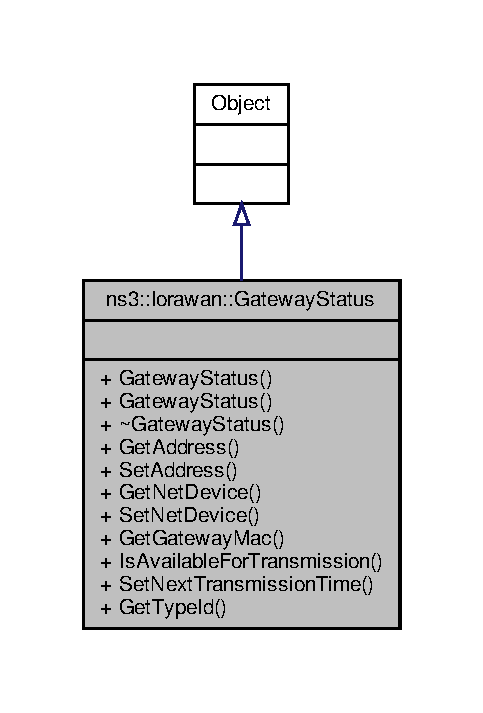
\includegraphics[width=232pt]{classns3_1_1lorawan_1_1GatewayStatus__inherit__graph}
\end{center}
\end{figure}


Collaboration diagram for ns3\+:\+:lorawan\+:\+:Gateway\+Status\+:
\nopagebreak
\begin{figure}[H]
\begin{center}
\leavevmode
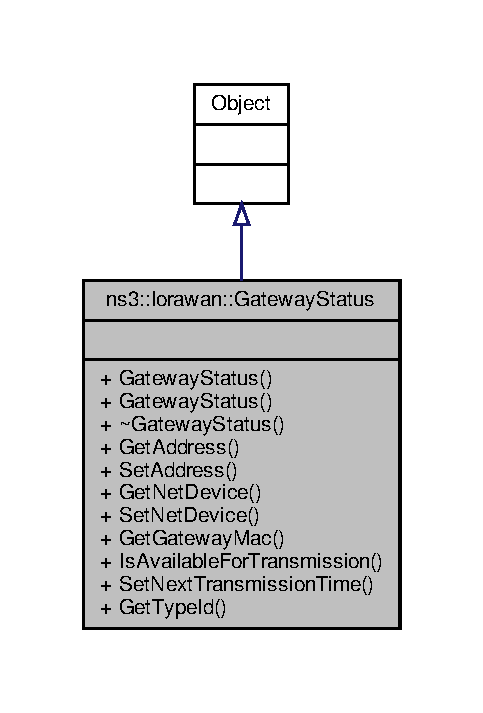
\includegraphics[width=232pt]{classns3_1_1lorawan_1_1GatewayStatus__coll__graph}
\end{center}
\end{figure}
\subsection*{Public Member Functions}
\begin{DoxyCompactItemize}
\item 
\mbox{\Hypertarget{classns3_1_1lorawan_1_1GatewayStatus_ade11dac71387dc888833792d271a38ff}\label{classns3_1_1lorawan_1_1GatewayStatus_ade11dac71387dc888833792d271a38ff}} 
{\bfseries Gateway\+Status} (Address address, Ptr$<$ \hyperlink{classNetDevice}{Net\+Device} $>$ net\+Device, Ptr$<$ \hyperlink{classns3_1_1lorawan_1_1GatewayLoraMac}{Gateway\+Lora\+Mac} $>$ gw\+Mac)
\item 
Address \hyperlink{classns3_1_1lorawan_1_1GatewayStatus_a0f90d708d60a10dcc768a1c84c995c0b}{Get\+Address} ()
\item 
void \hyperlink{classns3_1_1lorawan_1_1GatewayStatus_a073a26dbdcc6431a11ea774697925b1c}{Set\+Address} (Address address)
\item 
Ptr$<$ \hyperlink{classNetDevice}{Net\+Device} $>$ \hyperlink{classns3_1_1lorawan_1_1GatewayStatus_aaa7bdf07df771a98645d54d54144f4c2}{Get\+Net\+Device} ()
\item 
void \hyperlink{classns3_1_1lorawan_1_1GatewayStatus_af491570545959a7b8f1d0bb7228d520d}{Set\+Net\+Device} (Ptr$<$ \hyperlink{classNetDevice}{Net\+Device} $>$ net\+Device)
\item 
Ptr$<$ \hyperlink{classns3_1_1lorawan_1_1GatewayLoraMac}{Gateway\+Lora\+Mac} $>$ \hyperlink{classns3_1_1lorawan_1_1GatewayStatus_a4fb9662e38bf1007768dcebd033933a5}{Get\+Gateway\+Mac} (void)
\item 
bool \hyperlink{classns3_1_1lorawan_1_1GatewayStatus_a09aa68088ae7a91f6c215742eb2e5e6b}{Is\+Available\+For\+Transmission} (double frequency)
\item 
\mbox{\Hypertarget{classns3_1_1lorawan_1_1GatewayStatus_a5d3fd8f38c9ce48b3e3403fa72671723}\label{classns3_1_1lorawan_1_1GatewayStatus_a5d3fd8f38c9ce48b3e3403fa72671723}} 
void {\bfseries Set\+Next\+Transmission\+Time} (Time next\+Transmission\+Time)
\end{DoxyCompactItemize}
\subsection*{Static Public Member Functions}
\begin{DoxyCompactItemize}
\item 
\mbox{\Hypertarget{classns3_1_1lorawan_1_1GatewayStatus_a6e5beb75a9fde3f3cdc6f2fcec830b48}\label{classns3_1_1lorawan_1_1GatewayStatus_a6e5beb75a9fde3f3cdc6f2fcec830b48}} 
static Type\+Id {\bfseries Get\+Type\+Id} (void)
\end{DoxyCompactItemize}


\subsection{Member Function Documentation}
\mbox{\Hypertarget{classns3_1_1lorawan_1_1GatewayStatus_a0f90d708d60a10dcc768a1c84c995c0b}\label{classns3_1_1lorawan_1_1GatewayStatus_a0f90d708d60a10dcc768a1c84c995c0b}} 
\index{ns3\+::lorawan\+::\+Gateway\+Status@{ns3\+::lorawan\+::\+Gateway\+Status}!Get\+Address@{Get\+Address}}
\index{Get\+Address@{Get\+Address}!ns3\+::lorawan\+::\+Gateway\+Status@{ns3\+::lorawan\+::\+Gateway\+Status}}
\subsubsection{\texorpdfstring{Get\+Address()}{GetAddress()}}
{\footnotesize\ttfamily Address ns3\+::lorawan\+::\+Gateway\+Status\+::\+Get\+Address (\begin{DoxyParamCaption}{ }\end{DoxyParamCaption})}

Get this gateway\textquotesingle{}s P2P link address. \mbox{\Hypertarget{classns3_1_1lorawan_1_1GatewayStatus_a4fb9662e38bf1007768dcebd033933a5}\label{classns3_1_1lorawan_1_1GatewayStatus_a4fb9662e38bf1007768dcebd033933a5}} 
\index{ns3\+::lorawan\+::\+Gateway\+Status@{ns3\+::lorawan\+::\+Gateway\+Status}!Get\+Gateway\+Mac@{Get\+Gateway\+Mac}}
\index{Get\+Gateway\+Mac@{Get\+Gateway\+Mac}!ns3\+::lorawan\+::\+Gateway\+Status@{ns3\+::lorawan\+::\+Gateway\+Status}}
\subsubsection{\texorpdfstring{Get\+Gateway\+Mac()}{GetGatewayMac()}}
{\footnotesize\ttfamily Ptr$<$ \hyperlink{classns3_1_1lorawan_1_1GatewayLoraMac}{Gateway\+Lora\+Mac} $>$ ns3\+::lorawan\+::\+Gateway\+Status\+::\+Get\+Gateway\+Mac (\begin{DoxyParamCaption}\item[{void}]{ }\end{DoxyParamCaption})}

Get a pointer to this gateway\textquotesingle{}s M\+AC instance. \mbox{\Hypertarget{classns3_1_1lorawan_1_1GatewayStatus_aaa7bdf07df771a98645d54d54144f4c2}\label{classns3_1_1lorawan_1_1GatewayStatus_aaa7bdf07df771a98645d54d54144f4c2}} 
\index{ns3\+::lorawan\+::\+Gateway\+Status@{ns3\+::lorawan\+::\+Gateway\+Status}!Get\+Net\+Device@{Get\+Net\+Device}}
\index{Get\+Net\+Device@{Get\+Net\+Device}!ns3\+::lorawan\+::\+Gateway\+Status@{ns3\+::lorawan\+::\+Gateway\+Status}}
\subsubsection{\texorpdfstring{Get\+Net\+Device()}{GetNetDevice()}}
{\footnotesize\ttfamily Ptr$<$ \hyperlink{classNetDevice}{Net\+Device} $>$ ns3\+::lorawan\+::\+Gateway\+Status\+::\+Get\+Net\+Device (\begin{DoxyParamCaption}{ }\end{DoxyParamCaption})}

Get the \hyperlink{classNetDevice}{Net\+Device} through which it\textquotesingle{}s possible to contact this gateway from the server. \mbox{\Hypertarget{classns3_1_1lorawan_1_1GatewayStatus_a09aa68088ae7a91f6c215742eb2e5e6b}\label{classns3_1_1lorawan_1_1GatewayStatus_a09aa68088ae7a91f6c215742eb2e5e6b}} 
\index{ns3\+::lorawan\+::\+Gateway\+Status@{ns3\+::lorawan\+::\+Gateway\+Status}!Is\+Available\+For\+Transmission@{Is\+Available\+For\+Transmission}}
\index{Is\+Available\+For\+Transmission@{Is\+Available\+For\+Transmission}!ns3\+::lorawan\+::\+Gateway\+Status@{ns3\+::lorawan\+::\+Gateway\+Status}}
\subsubsection{\texorpdfstring{Is\+Available\+For\+Transmission()}{IsAvailableForTransmission()}}
{\footnotesize\ttfamily bool ns3\+::lorawan\+::\+Gateway\+Status\+::\+Is\+Available\+For\+Transmission (\begin{DoxyParamCaption}\item[{double}]{frequency }\end{DoxyParamCaption})}

Set a pointer to this gateway\textquotesingle{}s M\+AC instance. Query whether or not this gateway is available for immediate transmission on this frequency.


\begin{DoxyParams}{Parameters}
{\em frequency} & The frequency at which the gateway\textquotesingle{}s availability should be queried. \\
\hline
\end{DoxyParams}
\begin{DoxyReturn}{Returns}
True if the gateway\textquotesingle{}s available, false otherwise. 
\end{DoxyReturn}
\mbox{\Hypertarget{classns3_1_1lorawan_1_1GatewayStatus_a073a26dbdcc6431a11ea774697925b1c}\label{classns3_1_1lorawan_1_1GatewayStatus_a073a26dbdcc6431a11ea774697925b1c}} 
\index{ns3\+::lorawan\+::\+Gateway\+Status@{ns3\+::lorawan\+::\+Gateway\+Status}!Set\+Address@{Set\+Address}}
\index{Set\+Address@{Set\+Address}!ns3\+::lorawan\+::\+Gateway\+Status@{ns3\+::lorawan\+::\+Gateway\+Status}}
\subsubsection{\texorpdfstring{Set\+Address()}{SetAddress()}}
{\footnotesize\ttfamily void ns3\+::lorawan\+::\+Gateway\+Status\+::\+Set\+Address (\begin{DoxyParamCaption}\item[{Address}]{address }\end{DoxyParamCaption})}

Set this gateway\textquotesingle{}s P2P link address. \mbox{\Hypertarget{classns3_1_1lorawan_1_1GatewayStatus_af491570545959a7b8f1d0bb7228d520d}\label{classns3_1_1lorawan_1_1GatewayStatus_af491570545959a7b8f1d0bb7228d520d}} 
\index{ns3\+::lorawan\+::\+Gateway\+Status@{ns3\+::lorawan\+::\+Gateway\+Status}!Set\+Net\+Device@{Set\+Net\+Device}}
\index{Set\+Net\+Device@{Set\+Net\+Device}!ns3\+::lorawan\+::\+Gateway\+Status@{ns3\+::lorawan\+::\+Gateway\+Status}}
\subsubsection{\texorpdfstring{Set\+Net\+Device()}{SetNetDevice()}}
{\footnotesize\ttfamily void ns3\+::lorawan\+::\+Gateway\+Status\+::\+Set\+Net\+Device (\begin{DoxyParamCaption}\item[{Ptr$<$ \hyperlink{classNetDevice}{Net\+Device} $>$}]{net\+Device }\end{DoxyParamCaption})}

Set the \hyperlink{classNetDevice}{Net\+Device} through which it\textquotesingle{}s possible to contact this gateway from the server. 

The documentation for this class was generated from the following files\+:\begin{DoxyCompactItemize}
\item 
gateway-\/status.\+h\item 
gateway-\/status.\+cc\end{DoxyCompactItemize}

\hypertarget{classHeader}{}\section{Header Class Reference}
\label{classHeader}\index{Header@{Header}}


Inheritance diagram for Header\+:
\nopagebreak
\begin{figure}[H]
\begin{center}
\leavevmode
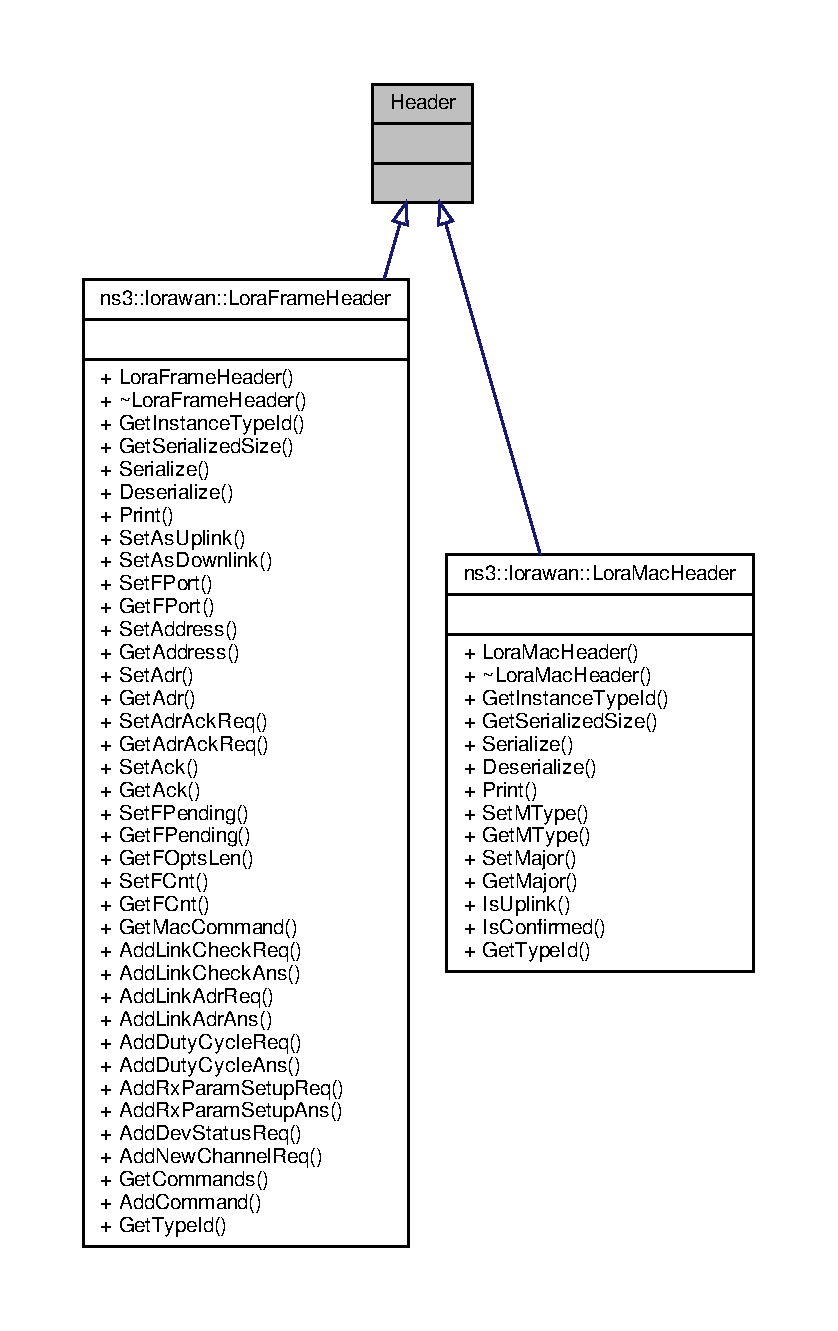
\includegraphics[height=550pt]{classHeader__inherit__graph}
\end{center}
\end{figure}


Collaboration diagram for Header\+:
\nopagebreak
\begin{figure}[H]
\begin{center}
\leavevmode
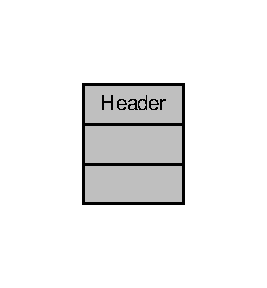
\includegraphics[width=128pt]{classHeader__coll__graph}
\end{center}
\end{figure}


The documentation for this class was generated from the following file\+:\begin{DoxyCompactItemize}
\item 
lora-\/mac-\/header.\+h\end{DoxyCompactItemize}

\hypertarget{classns3_1_1lorawan_1_1LinearLoraTxCurrentModel}{}\section{ns3\+:\+:lorawan\+:\+:Linear\+Lora\+Tx\+Current\+Model Class Reference}
\label{classns3_1_1lorawan_1_1LinearLoraTxCurrentModel}\index{ns3\+::lorawan\+::\+Linear\+Lora\+Tx\+Current\+Model@{ns3\+::lorawan\+::\+Linear\+Lora\+Tx\+Current\+Model}}


{\ttfamily \#include $<$lora-\/tx-\/current-\/model.\+h$>$}



Inheritance diagram for ns3\+:\+:lorawan\+:\+:Linear\+Lora\+Tx\+Current\+Model\+:
\nopagebreak
\begin{figure}[H]
\begin{center}
\leavevmode
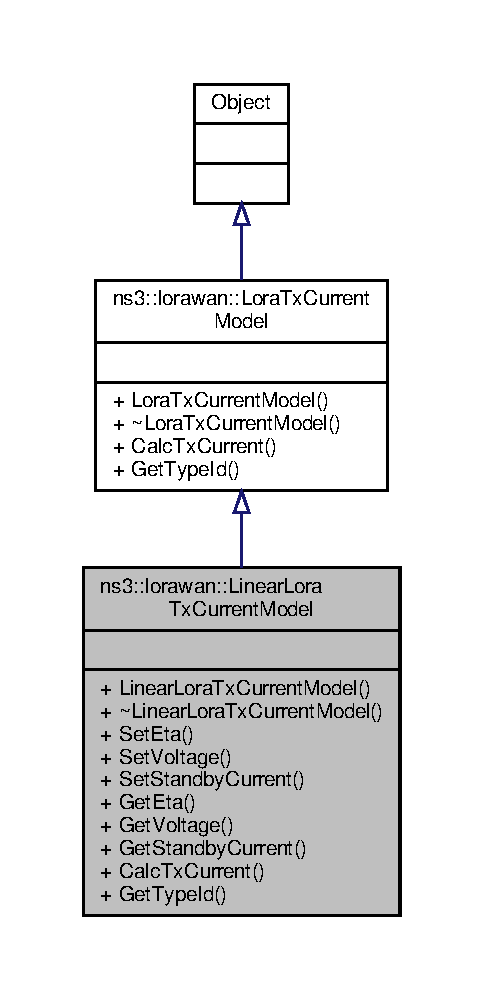
\includegraphics[width=232pt]{classns3_1_1lorawan_1_1LinearLoraTxCurrentModel__inherit__graph}
\end{center}
\end{figure}


Collaboration diagram for ns3\+:\+:lorawan\+:\+:Linear\+Lora\+Tx\+Current\+Model\+:
\nopagebreak
\begin{figure}[H]
\begin{center}
\leavevmode
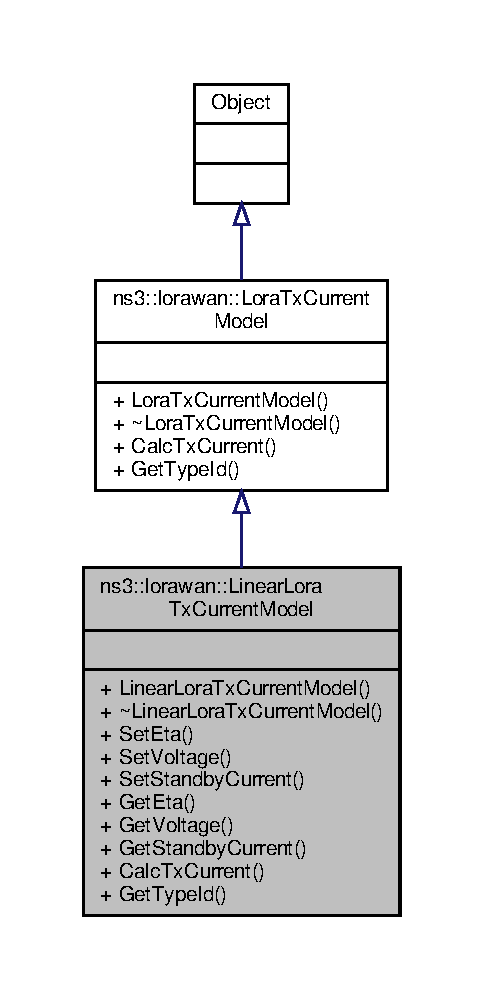
\includegraphics[width=232pt]{classns3_1_1lorawan_1_1LinearLoraTxCurrentModel__coll__graph}
\end{center}
\end{figure}
\subsection*{Public Member Functions}
\begin{DoxyCompactItemize}
\item 
void \hyperlink{classns3_1_1lorawan_1_1LinearLoraTxCurrentModel_adde65b755e155cba2f3cf7dd676d19df}{Set\+Eta} (double eta)
\item 
void \hyperlink{classns3_1_1lorawan_1_1LinearLoraTxCurrentModel_a675cff436187a271b78832f938b1d404}{Set\+Voltage} (double voltage)
\item 
void \hyperlink{classns3_1_1lorawan_1_1LinearLoraTxCurrentModel_a1685530e7d61367adfab611f724f95ce}{Set\+Standby\+Current} (double idle\+Current)
\item 
double \hyperlink{classns3_1_1lorawan_1_1LinearLoraTxCurrentModel_a4e15519375a8f9b0a43cc5e437461e5a}{Get\+Eta} (void) const
\item 
double \hyperlink{classns3_1_1lorawan_1_1LinearLoraTxCurrentModel_a74f4d04511937d792a90c69997773d95}{Get\+Voltage} (void) const
\item 
double \hyperlink{classns3_1_1lorawan_1_1LinearLoraTxCurrentModel_a74cf9badafdd63a68f40f8d3cb9898cb}{Get\+Standby\+Current} (void) const
\item 
double \hyperlink{classns3_1_1lorawan_1_1LinearLoraTxCurrentModel_a665f1751a87d6ff09b30c4ca30484b92}{Calc\+Tx\+Current} (double tx\+Power\+Dbm) const
\end{DoxyCompactItemize}
\subsection*{Static Public Member Functions}
\begin{DoxyCompactItemize}
\item 
\mbox{\Hypertarget{classns3_1_1lorawan_1_1LinearLoraTxCurrentModel_a910ea8ed64df92fcbd89e6a4b68ad03f}\label{classns3_1_1lorawan_1_1LinearLoraTxCurrentModel_a910ea8ed64df92fcbd89e6a4b68ad03f}} 
static Type\+Id {\bfseries Get\+Type\+Id} (void)
\end{DoxyCompactItemize}


\subsection{Detailed Description}
A linear model of the transmission current for a Lo\+Ra device, based on the Wi\+Fi model. 

\subsection{Member Function Documentation}
\mbox{\Hypertarget{classns3_1_1lorawan_1_1LinearLoraTxCurrentModel_a665f1751a87d6ff09b30c4ca30484b92}\label{classns3_1_1lorawan_1_1LinearLoraTxCurrentModel_a665f1751a87d6ff09b30c4ca30484b92}} 
\index{ns3\+::lorawan\+::\+Linear\+Lora\+Tx\+Current\+Model@{ns3\+::lorawan\+::\+Linear\+Lora\+Tx\+Current\+Model}!Calc\+Tx\+Current@{Calc\+Tx\+Current}}
\index{Calc\+Tx\+Current@{Calc\+Tx\+Current}!ns3\+::lorawan\+::\+Linear\+Lora\+Tx\+Current\+Model@{ns3\+::lorawan\+::\+Linear\+Lora\+Tx\+Current\+Model}}
\subsubsection{\texorpdfstring{Calc\+Tx\+Current()}{CalcTxCurrent()}}
{\footnotesize\ttfamily double ns3\+::lorawan\+::\+Linear\+Lora\+Tx\+Current\+Model\+::\+Calc\+Tx\+Current (\begin{DoxyParamCaption}\item[{double}]{tx\+Power\+Dbm }\end{DoxyParamCaption}) const\hspace{0.3cm}{\ttfamily [virtual]}}

Get the current for transmission at this power.


\begin{DoxyParams}{Parameters}
{\em tx\+Power\+Dbm} & The nominal tx power in d\+Bm \\
\hline
\end{DoxyParams}
\begin{DoxyReturn}{Returns}
The transmit current (in Ampere) 
\end{DoxyReturn}


Implements \hyperlink{classns3_1_1lorawan_1_1LoraTxCurrentModel_ad4143a40cb10d4cbd4bf838e006780c7}{ns3\+::lorawan\+::\+Lora\+Tx\+Current\+Model}.

\mbox{\Hypertarget{classns3_1_1lorawan_1_1LinearLoraTxCurrentModel_a4e15519375a8f9b0a43cc5e437461e5a}\label{classns3_1_1lorawan_1_1LinearLoraTxCurrentModel_a4e15519375a8f9b0a43cc5e437461e5a}} 
\index{ns3\+::lorawan\+::\+Linear\+Lora\+Tx\+Current\+Model@{ns3\+::lorawan\+::\+Linear\+Lora\+Tx\+Current\+Model}!Get\+Eta@{Get\+Eta}}
\index{Get\+Eta@{Get\+Eta}!ns3\+::lorawan\+::\+Linear\+Lora\+Tx\+Current\+Model@{ns3\+::lorawan\+::\+Linear\+Lora\+Tx\+Current\+Model}}
\subsubsection{\texorpdfstring{Get\+Eta()}{GetEta()}}
{\footnotesize\ttfamily double ns3\+::lorawan\+::\+Linear\+Lora\+Tx\+Current\+Model\+::\+Get\+Eta (\begin{DoxyParamCaption}\item[{void}]{ }\end{DoxyParamCaption}) const}

\begin{DoxyReturn}{Returns}
the power amplifier efficiency. 
\end{DoxyReturn}
\mbox{\Hypertarget{classns3_1_1lorawan_1_1LinearLoraTxCurrentModel_a74cf9badafdd63a68f40f8d3cb9898cb}\label{classns3_1_1lorawan_1_1LinearLoraTxCurrentModel_a74cf9badafdd63a68f40f8d3cb9898cb}} 
\index{ns3\+::lorawan\+::\+Linear\+Lora\+Tx\+Current\+Model@{ns3\+::lorawan\+::\+Linear\+Lora\+Tx\+Current\+Model}!Get\+Standby\+Current@{Get\+Standby\+Current}}
\index{Get\+Standby\+Current@{Get\+Standby\+Current}!ns3\+::lorawan\+::\+Linear\+Lora\+Tx\+Current\+Model@{ns3\+::lorawan\+::\+Linear\+Lora\+Tx\+Current\+Model}}
\subsubsection{\texorpdfstring{Get\+Standby\+Current()}{GetStandbyCurrent()}}
{\footnotesize\ttfamily double ns3\+::lorawan\+::\+Linear\+Lora\+Tx\+Current\+Model\+::\+Get\+Standby\+Current (\begin{DoxyParamCaption}\item[{void}]{ }\end{DoxyParamCaption}) const}

\begin{DoxyReturn}{Returns}
the current in the S\+T\+A\+N\+D\+BY state. 
\end{DoxyReturn}
\mbox{\Hypertarget{classns3_1_1lorawan_1_1LinearLoraTxCurrentModel_a74f4d04511937d792a90c69997773d95}\label{classns3_1_1lorawan_1_1LinearLoraTxCurrentModel_a74f4d04511937d792a90c69997773d95}} 
\index{ns3\+::lorawan\+::\+Linear\+Lora\+Tx\+Current\+Model@{ns3\+::lorawan\+::\+Linear\+Lora\+Tx\+Current\+Model}!Get\+Voltage@{Get\+Voltage}}
\index{Get\+Voltage@{Get\+Voltage}!ns3\+::lorawan\+::\+Linear\+Lora\+Tx\+Current\+Model@{ns3\+::lorawan\+::\+Linear\+Lora\+Tx\+Current\+Model}}
\subsubsection{\texorpdfstring{Get\+Voltage()}{GetVoltage()}}
{\footnotesize\ttfamily double ns3\+::lorawan\+::\+Linear\+Lora\+Tx\+Current\+Model\+::\+Get\+Voltage (\begin{DoxyParamCaption}\item[{void}]{ }\end{DoxyParamCaption}) const}

\begin{DoxyReturn}{Returns}
the supply voltage. 
\end{DoxyReturn}
\mbox{\Hypertarget{classns3_1_1lorawan_1_1LinearLoraTxCurrentModel_adde65b755e155cba2f3cf7dd676d19df}\label{classns3_1_1lorawan_1_1LinearLoraTxCurrentModel_adde65b755e155cba2f3cf7dd676d19df}} 
\index{ns3\+::lorawan\+::\+Linear\+Lora\+Tx\+Current\+Model@{ns3\+::lorawan\+::\+Linear\+Lora\+Tx\+Current\+Model}!Set\+Eta@{Set\+Eta}}
\index{Set\+Eta@{Set\+Eta}!ns3\+::lorawan\+::\+Linear\+Lora\+Tx\+Current\+Model@{ns3\+::lorawan\+::\+Linear\+Lora\+Tx\+Current\+Model}}
\subsubsection{\texorpdfstring{Set\+Eta()}{SetEta()}}
{\footnotesize\ttfamily void ns3\+::lorawan\+::\+Linear\+Lora\+Tx\+Current\+Model\+::\+Set\+Eta (\begin{DoxyParamCaption}\item[{double}]{eta }\end{DoxyParamCaption})}


\begin{DoxyParams}{Parameters}
{\em eta} & (dimension-\/less)\\
\hline
\end{DoxyParams}
Set the power amplifier efficiency. \mbox{\Hypertarget{classns3_1_1lorawan_1_1LinearLoraTxCurrentModel_a1685530e7d61367adfab611f724f95ce}\label{classns3_1_1lorawan_1_1LinearLoraTxCurrentModel_a1685530e7d61367adfab611f724f95ce}} 
\index{ns3\+::lorawan\+::\+Linear\+Lora\+Tx\+Current\+Model@{ns3\+::lorawan\+::\+Linear\+Lora\+Tx\+Current\+Model}!Set\+Standby\+Current@{Set\+Standby\+Current}}
\index{Set\+Standby\+Current@{Set\+Standby\+Current}!ns3\+::lorawan\+::\+Linear\+Lora\+Tx\+Current\+Model@{ns3\+::lorawan\+::\+Linear\+Lora\+Tx\+Current\+Model}}
\subsubsection{\texorpdfstring{Set\+Standby\+Current()}{SetStandbyCurrent()}}
{\footnotesize\ttfamily void ns3\+::lorawan\+::\+Linear\+Lora\+Tx\+Current\+Model\+::\+Set\+Standby\+Current (\begin{DoxyParamCaption}\item[{double}]{idle\+Current }\end{DoxyParamCaption})}


\begin{DoxyParams}{Parameters}
{\em idle\+Current} & (Ampere)\\
\hline
\end{DoxyParams}
Set the current in the S\+T\+A\+N\+D\+BY state. \mbox{\Hypertarget{classns3_1_1lorawan_1_1LinearLoraTxCurrentModel_a675cff436187a271b78832f938b1d404}\label{classns3_1_1lorawan_1_1LinearLoraTxCurrentModel_a675cff436187a271b78832f938b1d404}} 
\index{ns3\+::lorawan\+::\+Linear\+Lora\+Tx\+Current\+Model@{ns3\+::lorawan\+::\+Linear\+Lora\+Tx\+Current\+Model}!Set\+Voltage@{Set\+Voltage}}
\index{Set\+Voltage@{Set\+Voltage}!ns3\+::lorawan\+::\+Linear\+Lora\+Tx\+Current\+Model@{ns3\+::lorawan\+::\+Linear\+Lora\+Tx\+Current\+Model}}
\subsubsection{\texorpdfstring{Set\+Voltage()}{SetVoltage()}}
{\footnotesize\ttfamily void ns3\+::lorawan\+::\+Linear\+Lora\+Tx\+Current\+Model\+::\+Set\+Voltage (\begin{DoxyParamCaption}\item[{double}]{voltage }\end{DoxyParamCaption})}


\begin{DoxyParams}{Parameters}
{\em voltage} & (Volts)\\
\hline
\end{DoxyParams}
Set the supply voltage. 

The documentation for this class was generated from the following files\+:\begin{DoxyCompactItemize}
\item 
lora-\/tx-\/current-\/model.\+h\item 
lora-\/tx-\/current-\/model.\+cc\end{DoxyCompactItemize}

\hypertarget{classns3_1_1lorawan_1_1LinkAdrAns}{}\section{ns3\+:\+:lorawan\+:\+:Link\+Adr\+Ans Class Reference}
\label{classns3_1_1lorawan_1_1LinkAdrAns}\index{ns3\+::lorawan\+::\+Link\+Adr\+Ans@{ns3\+::lorawan\+::\+Link\+Adr\+Ans}}


{\ttfamily \#include $<$mac-\/command.\+h$>$}



Inheritance diagram for ns3\+:\+:lorawan\+:\+:Link\+Adr\+Ans\+:
\nopagebreak
\begin{figure}[H]
\begin{center}
\leavevmode
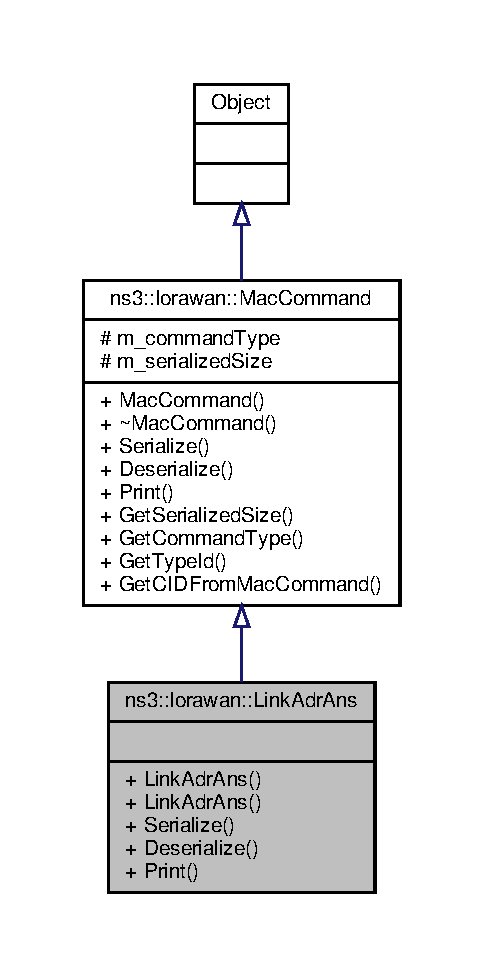
\includegraphics[width=232pt]{classns3_1_1lorawan_1_1LinkAdrAns__inherit__graph}
\end{center}
\end{figure}


Collaboration diagram for ns3\+:\+:lorawan\+:\+:Link\+Adr\+Ans\+:
\nopagebreak
\begin{figure}[H]
\begin{center}
\leavevmode
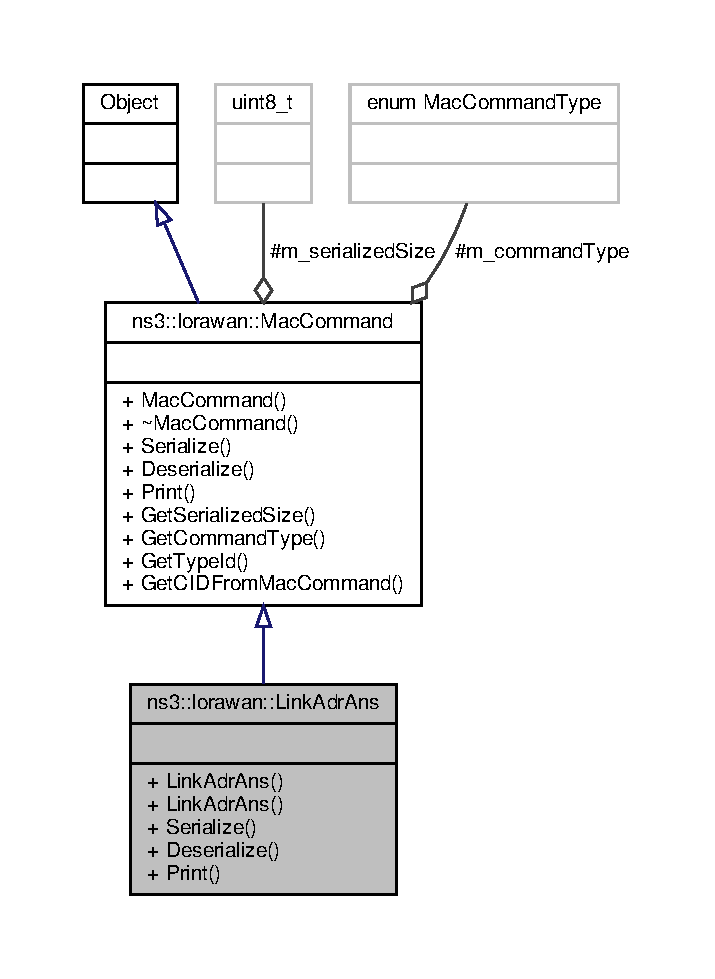
\includegraphics[width=343pt]{classns3_1_1lorawan_1_1LinkAdrAns__coll__graph}
\end{center}
\end{figure}
\subsection*{Public Member Functions}
\begin{DoxyCompactItemize}
\item 
\mbox{\Hypertarget{classns3_1_1lorawan_1_1LinkAdrAns_a6837feca5c8a4bf06c2b86e6b3854749}\label{classns3_1_1lorawan_1_1LinkAdrAns_a6837feca5c8a4bf06c2b86e6b3854749}} 
{\bfseries Link\+Adr\+Ans} (bool power\+Ack, bool data\+Rate\+Ack, bool channel\+Mask\+Ack)
\item 
virtual void \hyperlink{classns3_1_1lorawan_1_1LinkAdrAns_a057b6fc123d090cdd835c90760a883ca}{Serialize} (Buffer\+::\+Iterator \&start) const
\item 
virtual uint8\+\_\+t \hyperlink{classns3_1_1lorawan_1_1LinkAdrAns_a2d90637751496615710c55233a3480a6}{Deserialize} (Buffer\+::\+Iterator \&start)
\item 
virtual void \hyperlink{classns3_1_1lorawan_1_1LinkAdrAns_a91434c73f73c48f60c1fa2226278ca99}{Print} (std\+::ostream \&os) const
\end{DoxyCompactItemize}
\subsection*{Additional Inherited Members}


\subsection{Detailed Description}
Implementation of the \hyperlink{classns3_1_1lorawan_1_1LinkAdrAns}{Link\+Adr\+Ans} Lo\+Ra\+W\+AN M\+AC command.

With this command, the end device acknowledges a \hyperlink{classns3_1_1lorawan_1_1LinkAdrReq}{Link\+Adr\+Req}. 

\subsection{Member Function Documentation}
\mbox{\Hypertarget{classns3_1_1lorawan_1_1LinkAdrAns_a2d90637751496615710c55233a3480a6}\label{classns3_1_1lorawan_1_1LinkAdrAns_a2d90637751496615710c55233a3480a6}} 
\index{ns3\+::lorawan\+::\+Link\+Adr\+Ans@{ns3\+::lorawan\+::\+Link\+Adr\+Ans}!Deserialize@{Deserialize}}
\index{Deserialize@{Deserialize}!ns3\+::lorawan\+::\+Link\+Adr\+Ans@{ns3\+::lorawan\+::\+Link\+Adr\+Ans}}
\subsubsection{\texorpdfstring{Deserialize()}{Deserialize()}}
{\footnotesize\ttfamily uint8\+\_\+t ns3\+::lorawan\+::\+Link\+Adr\+Ans\+::\+Deserialize (\begin{DoxyParamCaption}\item[{Buffer\+::\+Iterator \&}]{start }\end{DoxyParamCaption})\hspace{0.3cm}{\ttfamily [virtual]}}

Deserialize the buffer into a M\+AC command.


\begin{DoxyParams}{Parameters}
{\em start} & A pointer to the buffer that contains the serialized command. \\
\hline
\end{DoxyParams}
\begin{DoxyReturn}{Returns}
the number of bytes that were consumed. 
\end{DoxyReturn}


Implements \hyperlink{classns3_1_1lorawan_1_1MacCommand_af12d223a71a67196bce498f1240eda75}{ns3\+::lorawan\+::\+Mac\+Command}.

\mbox{\Hypertarget{classns3_1_1lorawan_1_1LinkAdrAns_a91434c73f73c48f60c1fa2226278ca99}\label{classns3_1_1lorawan_1_1LinkAdrAns_a91434c73f73c48f60c1fa2226278ca99}} 
\index{ns3\+::lorawan\+::\+Link\+Adr\+Ans@{ns3\+::lorawan\+::\+Link\+Adr\+Ans}!Print@{Print}}
\index{Print@{Print}!ns3\+::lorawan\+::\+Link\+Adr\+Ans@{ns3\+::lorawan\+::\+Link\+Adr\+Ans}}
\subsubsection{\texorpdfstring{Print()}{Print()}}
{\footnotesize\ttfamily void ns3\+::lorawan\+::\+Link\+Adr\+Ans\+::\+Print (\begin{DoxyParamCaption}\item[{std\+::ostream \&}]{os }\end{DoxyParamCaption}) const\hspace{0.3cm}{\ttfamily [virtual]}}

Print the contents of this M\+AC command in human-\/readable format.


\begin{DoxyParams}{Parameters}
{\em os} & The std\+::ostream instance on which to print the M\+AC command. \\
\hline
\end{DoxyParams}


Implements \hyperlink{classns3_1_1lorawan_1_1MacCommand_a6bf88db38dab7dcd817811a9fb59f920}{ns3\+::lorawan\+::\+Mac\+Command}.

\mbox{\Hypertarget{classns3_1_1lorawan_1_1LinkAdrAns_a057b6fc123d090cdd835c90760a883ca}\label{classns3_1_1lorawan_1_1LinkAdrAns_a057b6fc123d090cdd835c90760a883ca}} 
\index{ns3\+::lorawan\+::\+Link\+Adr\+Ans@{ns3\+::lorawan\+::\+Link\+Adr\+Ans}!Serialize@{Serialize}}
\index{Serialize@{Serialize}!ns3\+::lorawan\+::\+Link\+Adr\+Ans@{ns3\+::lorawan\+::\+Link\+Adr\+Ans}}
\subsubsection{\texorpdfstring{Serialize()}{Serialize()}}
{\footnotesize\ttfamily void ns3\+::lorawan\+::\+Link\+Adr\+Ans\+::\+Serialize (\begin{DoxyParamCaption}\item[{Buffer\+::\+Iterator \&}]{start }\end{DoxyParamCaption}) const\hspace{0.3cm}{\ttfamily [virtual]}}

Serialize the contents of this M\+AC command into a buffer, according to the Lo\+Ra\+W\+AN standard.


\begin{DoxyParams}{Parameters}
{\em start} & A pointer to the buffer into which to serialize the command. \\
\hline
\end{DoxyParams}


Implements \hyperlink{classns3_1_1lorawan_1_1MacCommand_a0ed44b33942ddc3dc9694dc06ab0b87f}{ns3\+::lorawan\+::\+Mac\+Command}.



The documentation for this class was generated from the following files\+:\begin{DoxyCompactItemize}
\item 
mac-\/command.\+h\item 
mac-\/command.\+cc\end{DoxyCompactItemize}

\hypertarget{classns3_1_1lorawan_1_1LinkAdrReq}{}\section{ns3\+:\+:lorawan\+:\+:Link\+Adr\+Req Class Reference}
\label{classns3_1_1lorawan_1_1LinkAdrReq}\index{ns3\+::lorawan\+::\+Link\+Adr\+Req@{ns3\+::lorawan\+::\+Link\+Adr\+Req}}


{\ttfamily \#include $<$mac-\/command.\+h$>$}



Inheritance diagram for ns3\+:\+:lorawan\+:\+:Link\+Adr\+Req\+:
\nopagebreak
\begin{figure}[H]
\begin{center}
\leavevmode
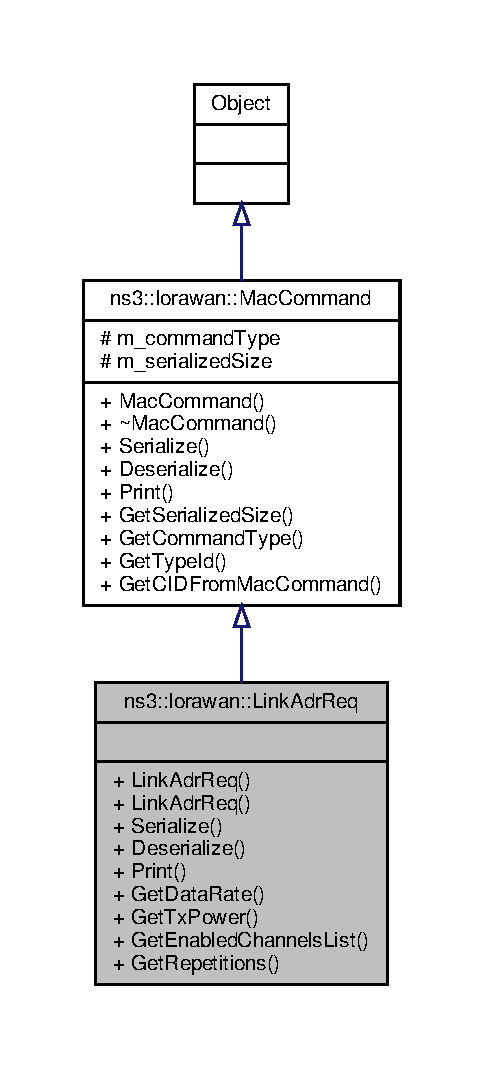
\includegraphics[width=232pt]{classns3_1_1lorawan_1_1LinkAdrReq__inherit__graph}
\end{center}
\end{figure}


Collaboration diagram for ns3\+:\+:lorawan\+:\+:Link\+Adr\+Req\+:
\nopagebreak
\begin{figure}[H]
\begin{center}
\leavevmode
\includegraphics[width=343pt]{classns3_1_1lorawan_1_1LinkAdrReq__coll__graph}
\end{center}
\end{figure}
\subsection*{Public Member Functions}
\begin{DoxyCompactItemize}
\item 
\mbox{\Hypertarget{classns3_1_1lorawan_1_1LinkAdrReq_a7eac381198a10a3e1ee4467d519a129a}\label{classns3_1_1lorawan_1_1LinkAdrReq_a7eac381198a10a3e1ee4467d519a129a}} 
{\bfseries Link\+Adr\+Req} (uint8\+\_\+t data\+Rate, uint8\+\_\+t tx\+Power, uint16\+\_\+t channel\+Mask, uint8\+\_\+t ch\+Mask\+Cntl, uint8\+\_\+t nb\+Rep)
\item 
virtual void \hyperlink{classns3_1_1lorawan_1_1LinkAdrReq_a92d99d7a9893de77be8bd14ef0109c53}{Serialize} (Buffer\+::\+Iterator \&start) const
\item 
virtual uint8\+\_\+t \hyperlink{classns3_1_1lorawan_1_1LinkAdrReq_abd1ff0ffcc32ec6a768e12eb18df2cee}{Deserialize} (Buffer\+::\+Iterator \&start)
\item 
virtual void \hyperlink{classns3_1_1lorawan_1_1LinkAdrReq_aa6f8732a740ae000006f56fd605cfaf4}{Print} (std\+::ostream \&os) const
\item 
uint8\+\_\+t \hyperlink{classns3_1_1lorawan_1_1LinkAdrReq_a21c567d9b65c39406555d42450d78018}{Get\+Data\+Rate} (void)
\item 
uint8\+\_\+t \hyperlink{classns3_1_1lorawan_1_1LinkAdrReq_a723eef40c7a4bba6f48d7ad61c2b9c12}{Get\+Tx\+Power} (void)
\item 
std\+::list$<$ int $>$ \hyperlink{classns3_1_1lorawan_1_1LinkAdrReq_a83aa5c208fb78807413451a87d67b6ec}{Get\+Enabled\+Channels\+List} (void)
\item 
int \hyperlink{classns3_1_1lorawan_1_1LinkAdrReq_acc3255bb562164ddd433f929e23a14d8}{Get\+Repetitions} (void)
\end{DoxyCompactItemize}
\subsection*{Additional Inherited Members}


\subsection{Detailed Description}
Implementation of the \hyperlink{classns3_1_1lorawan_1_1LinkAdrReq}{Link\+Adr\+Req} Lo\+Ra\+W\+AN M\+AC command.

With this command, the network server can request a device to change its data rate, transmission power and the channel it uses for uplink transmissions. 

\subsection{Member Function Documentation}
\mbox{\Hypertarget{classns3_1_1lorawan_1_1LinkAdrReq_abd1ff0ffcc32ec6a768e12eb18df2cee}\label{classns3_1_1lorawan_1_1LinkAdrReq_abd1ff0ffcc32ec6a768e12eb18df2cee}} 
\index{ns3\+::lorawan\+::\+Link\+Adr\+Req@{ns3\+::lorawan\+::\+Link\+Adr\+Req}!Deserialize@{Deserialize}}
\index{Deserialize@{Deserialize}!ns3\+::lorawan\+::\+Link\+Adr\+Req@{ns3\+::lorawan\+::\+Link\+Adr\+Req}}
\subsubsection{\texorpdfstring{Deserialize()}{Deserialize()}}
{\footnotesize\ttfamily uint8\+\_\+t ns3\+::lorawan\+::\+Link\+Adr\+Req\+::\+Deserialize (\begin{DoxyParamCaption}\item[{Buffer\+::\+Iterator \&}]{start }\end{DoxyParamCaption})\hspace{0.3cm}{\ttfamily [virtual]}}

Deserialize the buffer into a M\+AC command.


\begin{DoxyParams}{Parameters}
{\em start} & A pointer to the buffer that contains the serialized command. \\
\hline
\end{DoxyParams}
\begin{DoxyReturn}{Returns}
the number of bytes that were consumed. 
\end{DoxyReturn}


Implements \hyperlink{classns3_1_1lorawan_1_1MacCommand_af12d223a71a67196bce498f1240eda75}{ns3\+::lorawan\+::\+Mac\+Command}.

\mbox{\Hypertarget{classns3_1_1lorawan_1_1LinkAdrReq_a21c567d9b65c39406555d42450d78018}\label{classns3_1_1lorawan_1_1LinkAdrReq_a21c567d9b65c39406555d42450d78018}} 
\index{ns3\+::lorawan\+::\+Link\+Adr\+Req@{ns3\+::lorawan\+::\+Link\+Adr\+Req}!Get\+Data\+Rate@{Get\+Data\+Rate}}
\index{Get\+Data\+Rate@{Get\+Data\+Rate}!ns3\+::lorawan\+::\+Link\+Adr\+Req@{ns3\+::lorawan\+::\+Link\+Adr\+Req}}
\subsubsection{\texorpdfstring{Get\+Data\+Rate()}{GetDataRate()}}
{\footnotesize\ttfamily uint8\+\_\+t ns3\+::lorawan\+::\+Link\+Adr\+Req\+::\+Get\+Data\+Rate (\begin{DoxyParamCaption}\item[{void}]{ }\end{DoxyParamCaption})}

Return the data rate prescribed by this M\+AC command.

\begin{DoxyReturn}{Returns}
An unsigned 8-\/bit integer containing the data rate. 
\end{DoxyReturn}
\mbox{\Hypertarget{classns3_1_1lorawan_1_1LinkAdrReq_a83aa5c208fb78807413451a87d67b6ec}\label{classns3_1_1lorawan_1_1LinkAdrReq_a83aa5c208fb78807413451a87d67b6ec}} 
\index{ns3\+::lorawan\+::\+Link\+Adr\+Req@{ns3\+::lorawan\+::\+Link\+Adr\+Req}!Get\+Enabled\+Channels\+List@{Get\+Enabled\+Channels\+List}}
\index{Get\+Enabled\+Channels\+List@{Get\+Enabled\+Channels\+List}!ns3\+::lorawan\+::\+Link\+Adr\+Req@{ns3\+::lorawan\+::\+Link\+Adr\+Req}}
\subsubsection{\texorpdfstring{Get\+Enabled\+Channels\+List()}{GetEnabledChannelsList()}}
{\footnotesize\ttfamily std\+::list$<$ int $>$ ns3\+::lorawan\+::\+Link\+Adr\+Req\+::\+Get\+Enabled\+Channels\+List (\begin{DoxyParamCaption}\item[{void}]{ }\end{DoxyParamCaption})}

Get the list of enabled channels. This method takes the 16-\/bit channel mask and translates it to a list of integers that can be more easily parsed.

\begin{DoxyReturn}{Returns}
The list of enabled channels. 
\end{DoxyReturn}
\mbox{\Hypertarget{classns3_1_1lorawan_1_1LinkAdrReq_acc3255bb562164ddd433f929e23a14d8}\label{classns3_1_1lorawan_1_1LinkAdrReq_acc3255bb562164ddd433f929e23a14d8}} 
\index{ns3\+::lorawan\+::\+Link\+Adr\+Req@{ns3\+::lorawan\+::\+Link\+Adr\+Req}!Get\+Repetitions@{Get\+Repetitions}}
\index{Get\+Repetitions@{Get\+Repetitions}!ns3\+::lorawan\+::\+Link\+Adr\+Req@{ns3\+::lorawan\+::\+Link\+Adr\+Req}}
\subsubsection{\texorpdfstring{Get\+Repetitions()}{GetRepetitions()}}
{\footnotesize\ttfamily int ns3\+::lorawan\+::\+Link\+Adr\+Req\+::\+Get\+Repetitions (\begin{DoxyParamCaption}\item[{void}]{ }\end{DoxyParamCaption})}

Get the number of repetitions prescribed by this M\+AC command.

\begin{DoxyReturn}{Returns}
The number of repetitions. 
\end{DoxyReturn}
\mbox{\Hypertarget{classns3_1_1lorawan_1_1LinkAdrReq_a723eef40c7a4bba6f48d7ad61c2b9c12}\label{classns3_1_1lorawan_1_1LinkAdrReq_a723eef40c7a4bba6f48d7ad61c2b9c12}} 
\index{ns3\+::lorawan\+::\+Link\+Adr\+Req@{ns3\+::lorawan\+::\+Link\+Adr\+Req}!Get\+Tx\+Power@{Get\+Tx\+Power}}
\index{Get\+Tx\+Power@{Get\+Tx\+Power}!ns3\+::lorawan\+::\+Link\+Adr\+Req@{ns3\+::lorawan\+::\+Link\+Adr\+Req}}
\subsubsection{\texorpdfstring{Get\+Tx\+Power()}{GetTxPower()}}
{\footnotesize\ttfamily uint8\+\_\+t ns3\+::lorawan\+::\+Link\+Adr\+Req\+::\+Get\+Tx\+Power (\begin{DoxyParamCaption}\item[{void}]{ }\end{DoxyParamCaption})}

Get the transmission power prescribed by this M\+AC command.

The M\+AC layer is expected to translate this value to a certain power in d\+Bm when communicating it to the P\+HY, and the translation will vary based on the region of the device.

\begin{DoxyReturn}{Returns}
The TX power, encoded as an unsigned 8-\/bit integer. 
\end{DoxyReturn}
\mbox{\Hypertarget{classns3_1_1lorawan_1_1LinkAdrReq_aa6f8732a740ae000006f56fd605cfaf4}\label{classns3_1_1lorawan_1_1LinkAdrReq_aa6f8732a740ae000006f56fd605cfaf4}} 
\index{ns3\+::lorawan\+::\+Link\+Adr\+Req@{ns3\+::lorawan\+::\+Link\+Adr\+Req}!Print@{Print}}
\index{Print@{Print}!ns3\+::lorawan\+::\+Link\+Adr\+Req@{ns3\+::lorawan\+::\+Link\+Adr\+Req}}
\subsubsection{\texorpdfstring{Print()}{Print()}}
{\footnotesize\ttfamily void ns3\+::lorawan\+::\+Link\+Adr\+Req\+::\+Print (\begin{DoxyParamCaption}\item[{std\+::ostream \&}]{os }\end{DoxyParamCaption}) const\hspace{0.3cm}{\ttfamily [virtual]}}

Print the contents of this M\+AC command in human-\/readable format.


\begin{DoxyParams}{Parameters}
{\em os} & The std\+::ostream instance on which to print the M\+AC command. \\
\hline
\end{DoxyParams}


Implements \hyperlink{classns3_1_1lorawan_1_1MacCommand_a6bf88db38dab7dcd817811a9fb59f920}{ns3\+::lorawan\+::\+Mac\+Command}.

\mbox{\Hypertarget{classns3_1_1lorawan_1_1LinkAdrReq_a92d99d7a9893de77be8bd14ef0109c53}\label{classns3_1_1lorawan_1_1LinkAdrReq_a92d99d7a9893de77be8bd14ef0109c53}} 
\index{ns3\+::lorawan\+::\+Link\+Adr\+Req@{ns3\+::lorawan\+::\+Link\+Adr\+Req}!Serialize@{Serialize}}
\index{Serialize@{Serialize}!ns3\+::lorawan\+::\+Link\+Adr\+Req@{ns3\+::lorawan\+::\+Link\+Adr\+Req}}
\subsubsection{\texorpdfstring{Serialize()}{Serialize()}}
{\footnotesize\ttfamily void ns3\+::lorawan\+::\+Link\+Adr\+Req\+::\+Serialize (\begin{DoxyParamCaption}\item[{Buffer\+::\+Iterator \&}]{start }\end{DoxyParamCaption}) const\hspace{0.3cm}{\ttfamily [virtual]}}

Serialize the contents of this M\+AC command into a buffer, according to the Lo\+Ra\+W\+AN standard.


\begin{DoxyParams}{Parameters}
{\em start} & A pointer to the buffer into which to serialize the command. \\
\hline
\end{DoxyParams}


Implements \hyperlink{classns3_1_1lorawan_1_1MacCommand_a0ed44b33942ddc3dc9694dc06ab0b87f}{ns3\+::lorawan\+::\+Mac\+Command}.



The documentation for this class was generated from the following files\+:\begin{DoxyCompactItemize}
\item 
mac-\/command.\+h\item 
mac-\/command.\+cc\end{DoxyCompactItemize}

\hypertarget{classns3_1_1lorawan_1_1LinkCheckAns}{}\section{ns3\+:\+:lorawan\+:\+:Link\+Check\+Ans Class Reference}
\label{classns3_1_1lorawan_1_1LinkCheckAns}\index{ns3\+::lorawan\+::\+Link\+Check\+Ans@{ns3\+::lorawan\+::\+Link\+Check\+Ans}}


{\ttfamily \#include $<$mac-\/command.\+h$>$}



Inheritance diagram for ns3\+:\+:lorawan\+:\+:Link\+Check\+Ans\+:
\nopagebreak
\begin{figure}[H]
\begin{center}
\leavevmode
\includegraphics[width=232pt]{classns3_1_1lorawan_1_1LinkCheckAns__inherit__graph}
\end{center}
\end{figure}


Collaboration diagram for ns3\+:\+:lorawan\+:\+:Link\+Check\+Ans\+:
\nopagebreak
\begin{figure}[H]
\begin{center}
\leavevmode
\includegraphics[width=343pt]{classns3_1_1lorawan_1_1LinkCheckAns__coll__graph}
\end{center}
\end{figure}
\subsection*{Public Member Functions}
\begin{DoxyCompactItemize}
\item 
\mbox{\Hypertarget{classns3_1_1lorawan_1_1LinkCheckAns_a90b6b5ce1302e96dc9bfdce1e166a97f}\label{classns3_1_1lorawan_1_1LinkCheckAns_a90b6b5ce1302e96dc9bfdce1e166a97f}} 
{\bfseries Link\+Check\+Ans} (uint8\+\_\+t margin, uint8\+\_\+t gw\+Cnt)
\item 
virtual void \hyperlink{classns3_1_1lorawan_1_1LinkCheckAns_a54d7dcbbf322ece82652a5ac3603f83c}{Serialize} (Buffer\+::\+Iterator \&start) const
\item 
virtual uint8\+\_\+t \hyperlink{classns3_1_1lorawan_1_1LinkCheckAns_a6e3087a8b109129cb3e53f29625f9fbf}{Deserialize} (Buffer\+::\+Iterator \&start)
\item 
virtual void \hyperlink{classns3_1_1lorawan_1_1LinkCheckAns_a35637426df92297b70b3a7a1beae3326}{Print} (std\+::ostream \&os) const
\item 
void \hyperlink{classns3_1_1lorawan_1_1LinkCheckAns_af217ee3fe5287862f914c04a752672c2}{Set\+Margin} (uint8\+\_\+t margin)
\item 
uint8\+\_\+t \hyperlink{classns3_1_1lorawan_1_1LinkCheckAns_a95dcc4481a030e82f6f3ac12d391d6d5}{Get\+Margin} (void) const
\item 
void \hyperlink{classns3_1_1lorawan_1_1LinkCheckAns_afb84d89f6fa26b9f26250c54120d8f44}{Set\+Gw\+Cnt} (uint8\+\_\+t gw\+Cnt)
\item 
uint8\+\_\+t \hyperlink{classns3_1_1lorawan_1_1LinkCheckAns_a031c9ac33bfac632ff32b1cf2f67232a}{Get\+Gw\+Cnt} (void) const
\item 
void \hyperlink{classns3_1_1lorawan_1_1LinkCheckAns_a0439b17acc2140e08fa274c8199128d7}{Increment\+Gw\+Cnt} (void)
\end{DoxyCompactItemize}
\subsection*{Additional Inherited Members}


\subsection{Detailed Description}
Implementation of the \hyperlink{classns3_1_1lorawan_1_1LinkCheckAns}{Link\+Check\+Ans} Lo\+Ra\+W\+AN M\+AC command.

This command contains the demodulation margin and the number of receiving gateways of the packet containing the \hyperlink{classns3_1_1lorawan_1_1LinkCheckReq}{Link\+Check\+Req} command. 

\subsection{Member Function Documentation}
\mbox{\Hypertarget{classns3_1_1lorawan_1_1LinkCheckAns_a6e3087a8b109129cb3e53f29625f9fbf}\label{classns3_1_1lorawan_1_1LinkCheckAns_a6e3087a8b109129cb3e53f29625f9fbf}} 
\index{ns3\+::lorawan\+::\+Link\+Check\+Ans@{ns3\+::lorawan\+::\+Link\+Check\+Ans}!Deserialize@{Deserialize}}
\index{Deserialize@{Deserialize}!ns3\+::lorawan\+::\+Link\+Check\+Ans@{ns3\+::lorawan\+::\+Link\+Check\+Ans}}
\subsubsection{\texorpdfstring{Deserialize()}{Deserialize()}}
{\footnotesize\ttfamily uint8\+\_\+t ns3\+::lorawan\+::\+Link\+Check\+Ans\+::\+Deserialize (\begin{DoxyParamCaption}\item[{Buffer\+::\+Iterator \&}]{start }\end{DoxyParamCaption})\hspace{0.3cm}{\ttfamily [virtual]}}

Deserialize the buffer into a M\+AC command.


\begin{DoxyParams}{Parameters}
{\em start} & A pointer to the buffer that contains the serialized command. \\
\hline
\end{DoxyParams}
\begin{DoxyReturn}{Returns}
the number of bytes that were consumed. 
\end{DoxyReturn}


Implements \hyperlink{classns3_1_1lorawan_1_1MacCommand_af12d223a71a67196bce498f1240eda75}{ns3\+::lorawan\+::\+Mac\+Command}.

\mbox{\Hypertarget{classns3_1_1lorawan_1_1LinkCheckAns_a031c9ac33bfac632ff32b1cf2f67232a}\label{classns3_1_1lorawan_1_1LinkCheckAns_a031c9ac33bfac632ff32b1cf2f67232a}} 
\index{ns3\+::lorawan\+::\+Link\+Check\+Ans@{ns3\+::lorawan\+::\+Link\+Check\+Ans}!Get\+Gw\+Cnt@{Get\+Gw\+Cnt}}
\index{Get\+Gw\+Cnt@{Get\+Gw\+Cnt}!ns3\+::lorawan\+::\+Link\+Check\+Ans@{ns3\+::lorawan\+::\+Link\+Check\+Ans}}
\subsubsection{\texorpdfstring{Get\+Gw\+Cnt()}{GetGwCnt()}}
{\footnotesize\ttfamily uint8\+\_\+t ns3\+::lorawan\+::\+Link\+Check\+Ans\+::\+Get\+Gw\+Cnt (\begin{DoxyParamCaption}\item[{void}]{ }\end{DoxyParamCaption}) const}

Get the gateway count value.

\begin{DoxyReturn}{Returns}
The gateway count value. 
\end{DoxyReturn}
\mbox{\Hypertarget{classns3_1_1lorawan_1_1LinkCheckAns_a95dcc4481a030e82f6f3ac12d391d6d5}\label{classns3_1_1lorawan_1_1LinkCheckAns_a95dcc4481a030e82f6f3ac12d391d6d5}} 
\index{ns3\+::lorawan\+::\+Link\+Check\+Ans@{ns3\+::lorawan\+::\+Link\+Check\+Ans}!Get\+Margin@{Get\+Margin}}
\index{Get\+Margin@{Get\+Margin}!ns3\+::lorawan\+::\+Link\+Check\+Ans@{ns3\+::lorawan\+::\+Link\+Check\+Ans}}
\subsubsection{\texorpdfstring{Get\+Margin()}{GetMargin()}}
{\footnotesize\ttfamily uint8\+\_\+t ns3\+::lorawan\+::\+Link\+Check\+Ans\+::\+Get\+Margin (\begin{DoxyParamCaption}\item[{void}]{ }\end{DoxyParamCaption}) const}

Get the demodulation margin value.

\begin{DoxyReturn}{Returns}
The demodulation margin value. 
\end{DoxyReturn}
\mbox{\Hypertarget{classns3_1_1lorawan_1_1LinkCheckAns_a0439b17acc2140e08fa274c8199128d7}\label{classns3_1_1lorawan_1_1LinkCheckAns_a0439b17acc2140e08fa274c8199128d7}} 
\index{ns3\+::lorawan\+::\+Link\+Check\+Ans@{ns3\+::lorawan\+::\+Link\+Check\+Ans}!Increment\+Gw\+Cnt@{Increment\+Gw\+Cnt}}
\index{Increment\+Gw\+Cnt@{Increment\+Gw\+Cnt}!ns3\+::lorawan\+::\+Link\+Check\+Ans@{ns3\+::lorawan\+::\+Link\+Check\+Ans}}
\subsubsection{\texorpdfstring{Increment\+Gw\+Cnt()}{IncrementGwCnt()}}
{\footnotesize\ttfamily void ns3\+::lorawan\+::\+Link\+Check\+Ans\+::\+Increment\+Gw\+Cnt (\begin{DoxyParamCaption}\item[{void}]{ }\end{DoxyParamCaption})}

Increment this \hyperlink{classns3_1_1lorawan_1_1MacCommand}{Mac\+Command}\textquotesingle{}s gw\+Cnt value. \mbox{\Hypertarget{classns3_1_1lorawan_1_1LinkCheckAns_a35637426df92297b70b3a7a1beae3326}\label{classns3_1_1lorawan_1_1LinkCheckAns_a35637426df92297b70b3a7a1beae3326}} 
\index{ns3\+::lorawan\+::\+Link\+Check\+Ans@{ns3\+::lorawan\+::\+Link\+Check\+Ans}!Print@{Print}}
\index{Print@{Print}!ns3\+::lorawan\+::\+Link\+Check\+Ans@{ns3\+::lorawan\+::\+Link\+Check\+Ans}}
\subsubsection{\texorpdfstring{Print()}{Print()}}
{\footnotesize\ttfamily void ns3\+::lorawan\+::\+Link\+Check\+Ans\+::\+Print (\begin{DoxyParamCaption}\item[{std\+::ostream \&}]{os }\end{DoxyParamCaption}) const\hspace{0.3cm}{\ttfamily [virtual]}}

Print the contents of this M\+AC command in human-\/readable format.


\begin{DoxyParams}{Parameters}
{\em os} & The std\+::ostream instance on which to print the M\+AC command. \\
\hline
\end{DoxyParams}


Implements \hyperlink{classns3_1_1lorawan_1_1MacCommand_a6bf88db38dab7dcd817811a9fb59f920}{ns3\+::lorawan\+::\+Mac\+Command}.

\mbox{\Hypertarget{classns3_1_1lorawan_1_1LinkCheckAns_a54d7dcbbf322ece82652a5ac3603f83c}\label{classns3_1_1lorawan_1_1LinkCheckAns_a54d7dcbbf322ece82652a5ac3603f83c}} 
\index{ns3\+::lorawan\+::\+Link\+Check\+Ans@{ns3\+::lorawan\+::\+Link\+Check\+Ans}!Serialize@{Serialize}}
\index{Serialize@{Serialize}!ns3\+::lorawan\+::\+Link\+Check\+Ans@{ns3\+::lorawan\+::\+Link\+Check\+Ans}}
\subsubsection{\texorpdfstring{Serialize()}{Serialize()}}
{\footnotesize\ttfamily void ns3\+::lorawan\+::\+Link\+Check\+Ans\+::\+Serialize (\begin{DoxyParamCaption}\item[{Buffer\+::\+Iterator \&}]{start }\end{DoxyParamCaption}) const\hspace{0.3cm}{\ttfamily [virtual]}}

Serialize the contents of this M\+AC command into a buffer, according to the Lo\+Ra\+W\+AN standard.


\begin{DoxyParams}{Parameters}
{\em start} & A pointer to the buffer into which to serialize the command. \\
\hline
\end{DoxyParams}


Implements \hyperlink{classns3_1_1lorawan_1_1MacCommand_a0ed44b33942ddc3dc9694dc06ab0b87f}{ns3\+::lorawan\+::\+Mac\+Command}.

\mbox{\Hypertarget{classns3_1_1lorawan_1_1LinkCheckAns_afb84d89f6fa26b9f26250c54120d8f44}\label{classns3_1_1lorawan_1_1LinkCheckAns_afb84d89f6fa26b9f26250c54120d8f44}} 
\index{ns3\+::lorawan\+::\+Link\+Check\+Ans@{ns3\+::lorawan\+::\+Link\+Check\+Ans}!Set\+Gw\+Cnt@{Set\+Gw\+Cnt}}
\index{Set\+Gw\+Cnt@{Set\+Gw\+Cnt}!ns3\+::lorawan\+::\+Link\+Check\+Ans@{ns3\+::lorawan\+::\+Link\+Check\+Ans}}
\subsubsection{\texorpdfstring{Set\+Gw\+Cnt()}{SetGwCnt()}}
{\footnotesize\ttfamily void ns3\+::lorawan\+::\+Link\+Check\+Ans\+::\+Set\+Gw\+Cnt (\begin{DoxyParamCaption}\item[{uint8\+\_\+t}]{gw\+Cnt }\end{DoxyParamCaption})}

Set the gateway count value.


\begin{DoxyParams}{Parameters}
{\em gw\+Cnt} & The count value to set. \\
\hline
\end{DoxyParams}
\mbox{\Hypertarget{classns3_1_1lorawan_1_1LinkCheckAns_af217ee3fe5287862f914c04a752672c2}\label{classns3_1_1lorawan_1_1LinkCheckAns_af217ee3fe5287862f914c04a752672c2}} 
\index{ns3\+::lorawan\+::\+Link\+Check\+Ans@{ns3\+::lorawan\+::\+Link\+Check\+Ans}!Set\+Margin@{Set\+Margin}}
\index{Set\+Margin@{Set\+Margin}!ns3\+::lorawan\+::\+Link\+Check\+Ans@{ns3\+::lorawan\+::\+Link\+Check\+Ans}}
\subsubsection{\texorpdfstring{Set\+Margin()}{SetMargin()}}
{\footnotesize\ttfamily void ns3\+::lorawan\+::\+Link\+Check\+Ans\+::\+Set\+Margin (\begin{DoxyParamCaption}\item[{uint8\+\_\+t}]{margin }\end{DoxyParamCaption})}

Set the demodulation margin value.


\begin{DoxyParams}{Parameters}
{\em margin} & The demodulation margin to set. \\
\hline
\end{DoxyParams}


The documentation for this class was generated from the following files\+:\begin{DoxyCompactItemize}
\item 
mac-\/command.\+h\item 
mac-\/command.\+cc\end{DoxyCompactItemize}

\hypertarget{classns3_1_1lorawan_1_1LinkCheckComponent}{}\section{ns3\+:\+:lorawan\+:\+:Link\+Check\+Component Class Reference}
\label{classns3_1_1lorawan_1_1LinkCheckComponent}\index{ns3\+::lorawan\+::\+Link\+Check\+Component@{ns3\+::lorawan\+::\+Link\+Check\+Component}}


Inheritance diagram for ns3\+:\+:lorawan\+:\+:Link\+Check\+Component\+:
\nopagebreak
\begin{figure}[H]
\begin{center}
\leavevmode
\includegraphics[width=255pt]{classns3_1_1lorawan_1_1LinkCheckComponent__inherit__graph}
\end{center}
\end{figure}


Collaboration diagram for ns3\+:\+:lorawan\+:\+:Link\+Check\+Component\+:
\nopagebreak
\begin{figure}[H]
\begin{center}
\leavevmode
\includegraphics[width=255pt]{classns3_1_1lorawan_1_1LinkCheckComponent__coll__graph}
\end{center}
\end{figure}
\subsection*{Public Member Functions}
\begin{DoxyCompactItemize}
\item 
void \hyperlink{classns3_1_1lorawan_1_1LinkCheckComponent_a3a17d37153329a0b52b58e8f79675611}{On\+Received\+Packet} (Ptr$<$ const Packet $>$ packet, Ptr$<$ \hyperlink{classns3_1_1lorawan_1_1EndDeviceStatus}{End\+Device\+Status} $>$ status, Ptr$<$ \hyperlink{classns3_1_1lorawan_1_1NetworkStatus}{Network\+Status} $>$ network\+Status)
\item 
\mbox{\Hypertarget{classns3_1_1lorawan_1_1LinkCheckComponent_aeae9ff3b922f090d4f0cb9397715e79b}\label{classns3_1_1lorawan_1_1LinkCheckComponent_aeae9ff3b922f090d4f0cb9397715e79b}} 
void {\bfseries Before\+Sending\+Reply} (Ptr$<$ \hyperlink{classns3_1_1lorawan_1_1EndDeviceStatus}{End\+Device\+Status} $>$ status, Ptr$<$ \hyperlink{classns3_1_1lorawan_1_1NetworkStatus}{Network\+Status} $>$ network\+Status)
\item 
void \hyperlink{classns3_1_1lorawan_1_1LinkCheckComponent_a256519f7da4d9d512ac1c1ce6bde4c1a}{On\+Failed\+Reply} (Ptr$<$ \hyperlink{classns3_1_1lorawan_1_1EndDeviceStatus}{End\+Device\+Status} $>$ status, Ptr$<$ \hyperlink{classns3_1_1lorawan_1_1NetworkStatus}{Network\+Status} $>$ network\+Status)
\end{DoxyCompactItemize}
\subsection*{Static Public Member Functions}
\begin{DoxyCompactItemize}
\item 
\mbox{\Hypertarget{classns3_1_1lorawan_1_1LinkCheckComponent_a6727e8475d22e64e2d24ef9da30e41a3}\label{classns3_1_1lorawan_1_1LinkCheckComponent_a6727e8475d22e64e2d24ef9da30e41a3}} 
static Type\+Id {\bfseries Get\+Type\+Id} (void)
\end{DoxyCompactItemize}


\subsection{Member Function Documentation}
\mbox{\Hypertarget{classns3_1_1lorawan_1_1LinkCheckComponent_a256519f7da4d9d512ac1c1ce6bde4c1a}\label{classns3_1_1lorawan_1_1LinkCheckComponent_a256519f7da4d9d512ac1c1ce6bde4c1a}} 
\index{ns3\+::lorawan\+::\+Link\+Check\+Component@{ns3\+::lorawan\+::\+Link\+Check\+Component}!On\+Failed\+Reply@{On\+Failed\+Reply}}
\index{On\+Failed\+Reply@{On\+Failed\+Reply}!ns3\+::lorawan\+::\+Link\+Check\+Component@{ns3\+::lorawan\+::\+Link\+Check\+Component}}
\subsubsection{\texorpdfstring{On\+Failed\+Reply()}{OnFailedReply()}}
{\footnotesize\ttfamily void ns3\+::lorawan\+::\+Link\+Check\+Component\+::\+On\+Failed\+Reply (\begin{DoxyParamCaption}\item[{Ptr$<$ \hyperlink{classns3_1_1lorawan_1_1EndDeviceStatus}{End\+Device\+Status} $>$}]{status,  }\item[{Ptr$<$ \hyperlink{classns3_1_1lorawan_1_1NetworkStatus}{Network\+Status} $>$}]{network\+Status }\end{DoxyParamCaption})\hspace{0.3cm}{\ttfamily [virtual]}}

Method that is called when a packet cannot be sent in the downlink.


\begin{DoxyParams}{Parameters}
{\em status} & The \hyperlink{classns3_1_1lorawan_1_1EndDeviceStatus}{End\+Device\+Status} of the device to which it was impossible to send a reply. \\
\hline
{\em network\+Status} & A pointer to the \hyperlink{classns3_1_1lorawan_1_1NetworkStatus}{Network\+Status} object \\
\hline
\end{DoxyParams}


Implements \hyperlink{classns3_1_1lorawan_1_1NetworkControllerComponent_aaff757f6ece10a8ef24564006c137d72}{ns3\+::lorawan\+::\+Network\+Controller\+Component}.

\mbox{\Hypertarget{classns3_1_1lorawan_1_1LinkCheckComponent_a3a17d37153329a0b52b58e8f79675611}\label{classns3_1_1lorawan_1_1LinkCheckComponent_a3a17d37153329a0b52b58e8f79675611}} 
\index{ns3\+::lorawan\+::\+Link\+Check\+Component@{ns3\+::lorawan\+::\+Link\+Check\+Component}!On\+Received\+Packet@{On\+Received\+Packet}}
\index{On\+Received\+Packet@{On\+Received\+Packet}!ns3\+::lorawan\+::\+Link\+Check\+Component@{ns3\+::lorawan\+::\+Link\+Check\+Component}}
\subsubsection{\texorpdfstring{On\+Received\+Packet()}{OnReceivedPacket()}}
{\footnotesize\ttfamily void ns3\+::lorawan\+::\+Link\+Check\+Component\+::\+On\+Received\+Packet (\begin{DoxyParamCaption}\item[{Ptr$<$ const Packet $>$}]{packet,  }\item[{Ptr$<$ \hyperlink{classns3_1_1lorawan_1_1EndDeviceStatus}{End\+Device\+Status} $>$}]{status,  }\item[{Ptr$<$ \hyperlink{classns3_1_1lorawan_1_1NetworkStatus}{Network\+Status} $>$}]{network\+Status }\end{DoxyParamCaption})\hspace{0.3cm}{\ttfamily [virtual]}}

This method checks whether the received packet requires an acknowledgment and sets up the appropriate reply in case it does.


\begin{DoxyParams}{Parameters}
{\em packet} & The newly received packet \\
\hline
{\em network\+Status} & A pointer to the \hyperlink{classns3_1_1lorawan_1_1NetworkStatus}{Network\+Status} object \\
\hline
\end{DoxyParams}


Implements \hyperlink{classns3_1_1lorawan_1_1NetworkControllerComponent_a965fb667c3e88703e8cdbcbcd057db6f}{ns3\+::lorawan\+::\+Network\+Controller\+Component}.



The documentation for this class was generated from the following files\+:\begin{DoxyCompactItemize}
\item 
network-\/controller-\/components.\+h\item 
network-\/controller-\/components.\+cc\end{DoxyCompactItemize}

\hypertarget{classns3_1_1lorawan_1_1LinkCheckReq}{}\section{ns3\+:\+:lorawan\+:\+:Link\+Check\+Req Class Reference}
\label{classns3_1_1lorawan_1_1LinkCheckReq}\index{ns3\+::lorawan\+::\+Link\+Check\+Req@{ns3\+::lorawan\+::\+Link\+Check\+Req}}


{\ttfamily \#include $<$mac-\/command.\+h$>$}



Inheritance diagram for ns3\+:\+:lorawan\+:\+:Link\+Check\+Req\+:
\nopagebreak
\begin{figure}[H]
\begin{center}
\leavevmode
\includegraphics[width=232pt]{classns3_1_1lorawan_1_1LinkCheckReq__inherit__graph}
\end{center}
\end{figure}


Collaboration diagram for ns3\+:\+:lorawan\+:\+:Link\+Check\+Req\+:
\nopagebreak
\begin{figure}[H]
\begin{center}
\leavevmode
\includegraphics[width=343pt]{classns3_1_1lorawan_1_1LinkCheckReq__coll__graph}
\end{center}
\end{figure}
\subsection*{Public Member Functions}
\begin{DoxyCompactItemize}
\item 
virtual void \hyperlink{classns3_1_1lorawan_1_1LinkCheckReq_a1be81dab18f22e357719385bb1f9fc46}{Serialize} (Buffer\+::\+Iterator \&start) const
\item 
virtual uint8\+\_\+t \hyperlink{classns3_1_1lorawan_1_1LinkCheckReq_aa628b654164b72a55daaaa831e27166e}{Deserialize} (Buffer\+::\+Iterator \&start)
\item 
virtual void \hyperlink{classns3_1_1lorawan_1_1LinkCheckReq_aa3a4fd54a54699ca3ec15ce608008fc3}{Print} (std\+::ostream \&os) const
\end{DoxyCompactItemize}
\subsection*{Additional Inherited Members}


\subsection{Detailed Description}
Implementation of the \hyperlink{classns3_1_1lorawan_1_1LinkCheckReq}{Link\+Check\+Req} Lo\+Ra\+W\+AN M\+AC command.

This command holds no variables, and just consists in the C\+ID. 

\subsection{Member Function Documentation}
\mbox{\Hypertarget{classns3_1_1lorawan_1_1LinkCheckReq_aa628b654164b72a55daaaa831e27166e}\label{classns3_1_1lorawan_1_1LinkCheckReq_aa628b654164b72a55daaaa831e27166e}} 
\index{ns3\+::lorawan\+::\+Link\+Check\+Req@{ns3\+::lorawan\+::\+Link\+Check\+Req}!Deserialize@{Deserialize}}
\index{Deserialize@{Deserialize}!ns3\+::lorawan\+::\+Link\+Check\+Req@{ns3\+::lorawan\+::\+Link\+Check\+Req}}
\subsubsection{\texorpdfstring{Deserialize()}{Deserialize()}}
{\footnotesize\ttfamily uint8\+\_\+t ns3\+::lorawan\+::\+Link\+Check\+Req\+::\+Deserialize (\begin{DoxyParamCaption}\item[{Buffer\+::\+Iterator \&}]{start }\end{DoxyParamCaption})\hspace{0.3cm}{\ttfamily [virtual]}}

Deserialize the buffer into a M\+AC command.


\begin{DoxyParams}{Parameters}
{\em start} & A pointer to the buffer that contains the serialized command. \\
\hline
\end{DoxyParams}
\begin{DoxyReturn}{Returns}
the number of bytes that were consumed. 
\end{DoxyReturn}


Implements \hyperlink{classns3_1_1lorawan_1_1MacCommand_af12d223a71a67196bce498f1240eda75}{ns3\+::lorawan\+::\+Mac\+Command}.

\mbox{\Hypertarget{classns3_1_1lorawan_1_1LinkCheckReq_aa3a4fd54a54699ca3ec15ce608008fc3}\label{classns3_1_1lorawan_1_1LinkCheckReq_aa3a4fd54a54699ca3ec15ce608008fc3}} 
\index{ns3\+::lorawan\+::\+Link\+Check\+Req@{ns3\+::lorawan\+::\+Link\+Check\+Req}!Print@{Print}}
\index{Print@{Print}!ns3\+::lorawan\+::\+Link\+Check\+Req@{ns3\+::lorawan\+::\+Link\+Check\+Req}}
\subsubsection{\texorpdfstring{Print()}{Print()}}
{\footnotesize\ttfamily void ns3\+::lorawan\+::\+Link\+Check\+Req\+::\+Print (\begin{DoxyParamCaption}\item[{std\+::ostream \&}]{os }\end{DoxyParamCaption}) const\hspace{0.3cm}{\ttfamily [virtual]}}

Print the contents of this M\+AC command in human-\/readable format.


\begin{DoxyParams}{Parameters}
{\em os} & The std\+::ostream instance on which to print the M\+AC command. \\
\hline
\end{DoxyParams}


Implements \hyperlink{classns3_1_1lorawan_1_1MacCommand_a6bf88db38dab7dcd817811a9fb59f920}{ns3\+::lorawan\+::\+Mac\+Command}.

\mbox{\Hypertarget{classns3_1_1lorawan_1_1LinkCheckReq_a1be81dab18f22e357719385bb1f9fc46}\label{classns3_1_1lorawan_1_1LinkCheckReq_a1be81dab18f22e357719385bb1f9fc46}} 
\index{ns3\+::lorawan\+::\+Link\+Check\+Req@{ns3\+::lorawan\+::\+Link\+Check\+Req}!Serialize@{Serialize}}
\index{Serialize@{Serialize}!ns3\+::lorawan\+::\+Link\+Check\+Req@{ns3\+::lorawan\+::\+Link\+Check\+Req}}
\subsubsection{\texorpdfstring{Serialize()}{Serialize()}}
{\footnotesize\ttfamily void ns3\+::lorawan\+::\+Link\+Check\+Req\+::\+Serialize (\begin{DoxyParamCaption}\item[{Buffer\+::\+Iterator \&}]{start }\end{DoxyParamCaption}) const\hspace{0.3cm}{\ttfamily [virtual]}}

Serialize the contents of this M\+AC command into a buffer, according to the Lo\+Ra\+W\+AN standard.


\begin{DoxyParams}{Parameters}
{\em start} & A pointer to the buffer into which to serialize the command. \\
\hline
\end{DoxyParams}


Implements \hyperlink{classns3_1_1lorawan_1_1MacCommand_a0ed44b33942ddc3dc9694dc06ab0b87f}{ns3\+::lorawan\+::\+Mac\+Command}.



The documentation for this class was generated from the following files\+:\begin{DoxyCompactItemize}
\item 
mac-\/command.\+h\item 
mac-\/command.\+cc\end{DoxyCompactItemize}

\hypertarget{classns3_1_1lorawan_1_1LogicalLoraChannel}{}\section{ns3\+:\+:lorawan\+:\+:Logical\+Lora\+Channel Class Reference}
\label{classns3_1_1lorawan_1_1LogicalLoraChannel}\index{ns3\+::lorawan\+::\+Logical\+Lora\+Channel@{ns3\+::lorawan\+::\+Logical\+Lora\+Channel}}


{\ttfamily \#include $<$logical-\/lora-\/channel.\+h$>$}



Inheritance diagram for ns3\+:\+:lorawan\+:\+:Logical\+Lora\+Channel\+:
\nopagebreak
\begin{figure}[H]
\begin{center}
\leavevmode
\includegraphics[width=212pt]{classns3_1_1lorawan_1_1LogicalLoraChannel__inherit__graph}
\end{center}
\end{figure}


Collaboration diagram for ns3\+:\+:lorawan\+:\+:Logical\+Lora\+Channel\+:
\nopagebreak
\begin{figure}[H]
\begin{center}
\leavevmode
\includegraphics[width=212pt]{classns3_1_1lorawan_1_1LogicalLoraChannel__coll__graph}
\end{center}
\end{figure}
\subsection*{Public Member Functions}
\begin{DoxyCompactItemize}
\item 
\mbox{\Hypertarget{classns3_1_1lorawan_1_1LogicalLoraChannel_af4804eb74b0d9e6b12a9321172d9296f}\label{classns3_1_1lorawan_1_1LogicalLoraChannel_af4804eb74b0d9e6b12a9321172d9296f}} 
{\bfseries Logical\+Lora\+Channel} (double frequency)
\item 
\hyperlink{classns3_1_1lorawan_1_1LogicalLoraChannel_a686e1cf42931f1df4b1de55eadd3abbe}{Logical\+Lora\+Channel} (double frequency, uint8\+\_\+t min\+Data\+Rate, uint8\+\_\+t max\+Data\+Rate)
\item 
double \hyperlink{classns3_1_1lorawan_1_1LogicalLoraChannel_af77fc25d0cf3f6e951e2e9b34464fb28}{Get\+Frequency} (void) const
\item 
void \hyperlink{classns3_1_1lorawan_1_1LogicalLoraChannel_a6e1a26e63f6eea84231a22bf7e99702c}{Set\+Minimum\+Data\+Rate} (uint8\+\_\+t min\+Data\+Rate)
\item 
void \hyperlink{classns3_1_1lorawan_1_1LogicalLoraChannel_ab8c110f44d5937fa0d3facd544551e60}{Set\+Maximum\+Data\+Rate} (uint8\+\_\+t max\+Data\+Rate)
\item 
uint8\+\_\+t \hyperlink{classns3_1_1lorawan_1_1LogicalLoraChannel_a1d8a54566ba09ca217a37cd29c568d13}{Get\+Minimum\+Data\+Rate} (void)
\item 
uint8\+\_\+t \hyperlink{classns3_1_1lorawan_1_1LogicalLoraChannel_a1dd2658114ee12032c5f8a28407349d1}{Get\+Maximum\+Data\+Rate} (void)
\item 
void \hyperlink{classns3_1_1lorawan_1_1LogicalLoraChannel_a94bbcfed3cd6f5b0df26229c284861be}{Set\+Enabled\+For\+Uplink} (void)
\item 
void \hyperlink{classns3_1_1lorawan_1_1LogicalLoraChannel_ac1dd87336f77086462816ceebd787b6c}{Disable\+For\+Uplink} (void)
\item 
bool \hyperlink{classns3_1_1lorawan_1_1LogicalLoraChannel_a05fd7f9703aad2b8657612fca09db0b9}{Is\+Enabled\+For\+Uplink} (void)
\end{DoxyCompactItemize}
\subsection*{Static Public Member Functions}
\begin{DoxyCompactItemize}
\item 
\mbox{\Hypertarget{classns3_1_1lorawan_1_1LogicalLoraChannel_affeafa2775461348be32c1670c65c005}\label{classns3_1_1lorawan_1_1LogicalLoraChannel_affeafa2775461348be32c1670c65c005}} 
static Type\+Id {\bfseries Get\+Type\+Id} (void)
\end{DoxyCompactItemize}


\subsection{Detailed Description}
This class represents a logical Lo\+Ra\+W\+AN channel.

A logical channel is characterized by a central frequency and a range of data rates that can be sent on it.

Furthermore, a \hyperlink{classns3_1_1lorawan_1_1LogicalLoraChannel}{Logical\+Lora\+Channel} can be marked as enabled or disabled for uplink transmission. 

\subsection{Constructor \& Destructor Documentation}
\mbox{\Hypertarget{classns3_1_1lorawan_1_1LogicalLoraChannel_a686e1cf42931f1df4b1de55eadd3abbe}\label{classns3_1_1lorawan_1_1LogicalLoraChannel_a686e1cf42931f1df4b1de55eadd3abbe}} 
\index{ns3\+::lorawan\+::\+Logical\+Lora\+Channel@{ns3\+::lorawan\+::\+Logical\+Lora\+Channel}!Logical\+Lora\+Channel@{Logical\+Lora\+Channel}}
\index{Logical\+Lora\+Channel@{Logical\+Lora\+Channel}!ns3\+::lorawan\+::\+Logical\+Lora\+Channel@{ns3\+::lorawan\+::\+Logical\+Lora\+Channel}}
\subsubsection{\texorpdfstring{Logical\+Lora\+Channel()}{LogicalLoraChannel()}}
{\footnotesize\ttfamily ns3\+::lorawan\+::\+Logical\+Lora\+Channel\+::\+Logical\+Lora\+Channel (\begin{DoxyParamCaption}\item[{double}]{frequency,  }\item[{uint8\+\_\+t}]{min\+Data\+Rate,  }\item[{uint8\+\_\+t}]{max\+Data\+Rate }\end{DoxyParamCaption})}

Constructor providing initialization of frequency and data rate limits.


\begin{DoxyParams}{Parameters}
{\em frequency} & This channel\textquotesingle{}s frequency. \\
\hline
{\em min\+Data\+Rate} & This channel\textquotesingle{}s minimum data rate. \\
\hline
{\em max\+Data\+Rate} & This channel\textquotesingle{}s maximum data rate. \\
\hline
\end{DoxyParams}


\subsection{Member Function Documentation}
\mbox{\Hypertarget{classns3_1_1lorawan_1_1LogicalLoraChannel_ac1dd87336f77086462816ceebd787b6c}\label{classns3_1_1lorawan_1_1LogicalLoraChannel_ac1dd87336f77086462816ceebd787b6c}} 
\index{ns3\+::lorawan\+::\+Logical\+Lora\+Channel@{ns3\+::lorawan\+::\+Logical\+Lora\+Channel}!Disable\+For\+Uplink@{Disable\+For\+Uplink}}
\index{Disable\+For\+Uplink@{Disable\+For\+Uplink}!ns3\+::lorawan\+::\+Logical\+Lora\+Channel@{ns3\+::lorawan\+::\+Logical\+Lora\+Channel}}
\subsubsection{\texorpdfstring{Disable\+For\+Uplink()}{DisableForUplink()}}
{\footnotesize\ttfamily void ns3\+::lorawan\+::\+Logical\+Lora\+Channel\+::\+Disable\+For\+Uplink (\begin{DoxyParamCaption}\item[{void}]{ }\end{DoxyParamCaption})}

Set this channel as disabled for uplink. \mbox{\Hypertarget{classns3_1_1lorawan_1_1LogicalLoraChannel_af77fc25d0cf3f6e951e2e9b34464fb28}\label{classns3_1_1lorawan_1_1LogicalLoraChannel_af77fc25d0cf3f6e951e2e9b34464fb28}} 
\index{ns3\+::lorawan\+::\+Logical\+Lora\+Channel@{ns3\+::lorawan\+::\+Logical\+Lora\+Channel}!Get\+Frequency@{Get\+Frequency}}
\index{Get\+Frequency@{Get\+Frequency}!ns3\+::lorawan\+::\+Logical\+Lora\+Channel@{ns3\+::lorawan\+::\+Logical\+Lora\+Channel}}
\subsubsection{\texorpdfstring{Get\+Frequency()}{GetFrequency()}}
{\footnotesize\ttfamily double ns3\+::lorawan\+::\+Logical\+Lora\+Channel\+::\+Get\+Frequency (\begin{DoxyParamCaption}\item[{void}]{ }\end{DoxyParamCaption}) const}

Get the frequency (M\+Hz).

\begin{DoxyReturn}{Returns}
The center frequency of this channel. 
\end{DoxyReturn}
\mbox{\Hypertarget{classns3_1_1lorawan_1_1LogicalLoraChannel_a1dd2658114ee12032c5f8a28407349d1}\label{classns3_1_1lorawan_1_1LogicalLoraChannel_a1dd2658114ee12032c5f8a28407349d1}} 
\index{ns3\+::lorawan\+::\+Logical\+Lora\+Channel@{ns3\+::lorawan\+::\+Logical\+Lora\+Channel}!Get\+Maximum\+Data\+Rate@{Get\+Maximum\+Data\+Rate}}
\index{Get\+Maximum\+Data\+Rate@{Get\+Maximum\+Data\+Rate}!ns3\+::lorawan\+::\+Logical\+Lora\+Channel@{ns3\+::lorawan\+::\+Logical\+Lora\+Channel}}
\subsubsection{\texorpdfstring{Get\+Maximum\+Data\+Rate()}{GetMaximumDataRate()}}
{\footnotesize\ttfamily uint8\+\_\+t ns3\+::lorawan\+::\+Logical\+Lora\+Channel\+::\+Get\+Maximum\+Data\+Rate (\begin{DoxyParamCaption}\item[{void}]{ }\end{DoxyParamCaption})}

Get the maximum Data Rate that is allowed on this channel. \mbox{\Hypertarget{classns3_1_1lorawan_1_1LogicalLoraChannel_a1d8a54566ba09ca217a37cd29c568d13}\label{classns3_1_1lorawan_1_1LogicalLoraChannel_a1d8a54566ba09ca217a37cd29c568d13}} 
\index{ns3\+::lorawan\+::\+Logical\+Lora\+Channel@{ns3\+::lorawan\+::\+Logical\+Lora\+Channel}!Get\+Minimum\+Data\+Rate@{Get\+Minimum\+Data\+Rate}}
\index{Get\+Minimum\+Data\+Rate@{Get\+Minimum\+Data\+Rate}!ns3\+::lorawan\+::\+Logical\+Lora\+Channel@{ns3\+::lorawan\+::\+Logical\+Lora\+Channel}}
\subsubsection{\texorpdfstring{Get\+Minimum\+Data\+Rate()}{GetMinimumDataRate()}}
{\footnotesize\ttfamily uint8\+\_\+t ns3\+::lorawan\+::\+Logical\+Lora\+Channel\+::\+Get\+Minimum\+Data\+Rate (\begin{DoxyParamCaption}\item[{void}]{ }\end{DoxyParamCaption})}

Get the minimum Data Rate that is allowed on this channel. \mbox{\Hypertarget{classns3_1_1lorawan_1_1LogicalLoraChannel_a05fd7f9703aad2b8657612fca09db0b9}\label{classns3_1_1lorawan_1_1LogicalLoraChannel_a05fd7f9703aad2b8657612fca09db0b9}} 
\index{ns3\+::lorawan\+::\+Logical\+Lora\+Channel@{ns3\+::lorawan\+::\+Logical\+Lora\+Channel}!Is\+Enabled\+For\+Uplink@{Is\+Enabled\+For\+Uplink}}
\index{Is\+Enabled\+For\+Uplink@{Is\+Enabled\+For\+Uplink}!ns3\+::lorawan\+::\+Logical\+Lora\+Channel@{ns3\+::lorawan\+::\+Logical\+Lora\+Channel}}
\subsubsection{\texorpdfstring{Is\+Enabled\+For\+Uplink()}{IsEnabledForUplink()}}
{\footnotesize\ttfamily bool ns3\+::lorawan\+::\+Logical\+Lora\+Channel\+::\+Is\+Enabled\+For\+Uplink (\begin{DoxyParamCaption}\item[{void}]{ }\end{DoxyParamCaption})}

Test whether this channel is marked as enabled for uplink. \mbox{\Hypertarget{classns3_1_1lorawan_1_1LogicalLoraChannel_a94bbcfed3cd6f5b0df26229c284861be}\label{classns3_1_1lorawan_1_1LogicalLoraChannel_a94bbcfed3cd6f5b0df26229c284861be}} 
\index{ns3\+::lorawan\+::\+Logical\+Lora\+Channel@{ns3\+::lorawan\+::\+Logical\+Lora\+Channel}!Set\+Enabled\+For\+Uplink@{Set\+Enabled\+For\+Uplink}}
\index{Set\+Enabled\+For\+Uplink@{Set\+Enabled\+For\+Uplink}!ns3\+::lorawan\+::\+Logical\+Lora\+Channel@{ns3\+::lorawan\+::\+Logical\+Lora\+Channel}}
\subsubsection{\texorpdfstring{Set\+Enabled\+For\+Uplink()}{SetEnabledForUplink()}}
{\footnotesize\ttfamily void ns3\+::lorawan\+::\+Logical\+Lora\+Channel\+::\+Set\+Enabled\+For\+Uplink (\begin{DoxyParamCaption}\item[{void}]{ }\end{DoxyParamCaption})}

Set this channel as enabled for uplink. \mbox{\Hypertarget{classns3_1_1lorawan_1_1LogicalLoraChannel_ab8c110f44d5937fa0d3facd544551e60}\label{classns3_1_1lorawan_1_1LogicalLoraChannel_ab8c110f44d5937fa0d3facd544551e60}} 
\index{ns3\+::lorawan\+::\+Logical\+Lora\+Channel@{ns3\+::lorawan\+::\+Logical\+Lora\+Channel}!Set\+Maximum\+Data\+Rate@{Set\+Maximum\+Data\+Rate}}
\index{Set\+Maximum\+Data\+Rate@{Set\+Maximum\+Data\+Rate}!ns3\+::lorawan\+::\+Logical\+Lora\+Channel@{ns3\+::lorawan\+::\+Logical\+Lora\+Channel}}
\subsubsection{\texorpdfstring{Set\+Maximum\+Data\+Rate()}{SetMaximumDataRate()}}
{\footnotesize\ttfamily void ns3\+::lorawan\+::\+Logical\+Lora\+Channel\+::\+Set\+Maximum\+Data\+Rate (\begin{DoxyParamCaption}\item[{uint8\+\_\+t}]{max\+Data\+Rate }\end{DoxyParamCaption})}

Set the maximum Data Rate that is allowed on this channel. \mbox{\Hypertarget{classns3_1_1lorawan_1_1LogicalLoraChannel_a6e1a26e63f6eea84231a22bf7e99702c}\label{classns3_1_1lorawan_1_1LogicalLoraChannel_a6e1a26e63f6eea84231a22bf7e99702c}} 
\index{ns3\+::lorawan\+::\+Logical\+Lora\+Channel@{ns3\+::lorawan\+::\+Logical\+Lora\+Channel}!Set\+Minimum\+Data\+Rate@{Set\+Minimum\+Data\+Rate}}
\index{Set\+Minimum\+Data\+Rate@{Set\+Minimum\+Data\+Rate}!ns3\+::lorawan\+::\+Logical\+Lora\+Channel@{ns3\+::lorawan\+::\+Logical\+Lora\+Channel}}
\subsubsection{\texorpdfstring{Set\+Minimum\+Data\+Rate()}{SetMinimumDataRate()}}
{\footnotesize\ttfamily void ns3\+::lorawan\+::\+Logical\+Lora\+Channel\+::\+Set\+Minimum\+Data\+Rate (\begin{DoxyParamCaption}\item[{uint8\+\_\+t}]{min\+Data\+Rate }\end{DoxyParamCaption})}

Set the frequency (M\+Hz).


\begin{DoxyParams}{Parameters}
{\em frequency\+M\+Hz} & The center frequency this channel should be at. Set the minimum Data Rate that is allowed on this channel. \\
\hline
\end{DoxyParams}


The documentation for this class was generated from the following files\+:\begin{DoxyCompactItemize}
\item 
logical-\/lora-\/channel.\+h\item 
logical-\/lora-\/channel.\+cc\end{DoxyCompactItemize}

\hypertarget{classns3_1_1lorawan_1_1LogicalLoraChannelHelper}{}\section{ns3\+:\+:lorawan\+:\+:Logical\+Lora\+Channel\+Helper Class Reference}
\label{classns3_1_1lorawan_1_1LogicalLoraChannelHelper}\index{ns3\+::lorawan\+::\+Logical\+Lora\+Channel\+Helper@{ns3\+::lorawan\+::\+Logical\+Lora\+Channel\+Helper}}


{\ttfamily \#include $<$logical-\/lora-\/channel-\/helper.\+h$>$}



Inheritance diagram for ns3\+:\+:lorawan\+:\+:Logical\+Lora\+Channel\+Helper\+:
\nopagebreak
\begin{figure}[H]
\begin{center}
\leavevmode
\includegraphics[width=235pt]{classns3_1_1lorawan_1_1LogicalLoraChannelHelper__inherit__graph}
\end{center}
\end{figure}


Collaboration diagram for ns3\+:\+:lorawan\+:\+:Logical\+Lora\+Channel\+Helper\+:
\nopagebreak
\begin{figure}[H]
\begin{center}
\leavevmode
\includegraphics[width=235pt]{classns3_1_1lorawan_1_1LogicalLoraChannelHelper__coll__graph}
\end{center}
\end{figure}
\subsection*{Public Member Functions}
\begin{DoxyCompactItemize}
\item 
Time \hyperlink{classns3_1_1lorawan_1_1LogicalLoraChannelHelper_a532db364466139b87e62c07cb2a85414}{Get\+Aggregated\+Waiting\+Time} (void)
\item 
Time \hyperlink{classns3_1_1lorawan_1_1LogicalLoraChannelHelper_ae4467bd31813cf74dcac7f4990f5aa15}{Get\+Waiting\+Time} (Ptr$<$ \hyperlink{classns3_1_1lorawan_1_1LogicalLoraChannel}{Logical\+Lora\+Channel} $>$ channel)
\item 
void \hyperlink{classns3_1_1lorawan_1_1LogicalLoraChannelHelper_ae48a646b236962de394678f054d5fc7b}{Add\+Event} (Time duration, Ptr$<$ \hyperlink{classns3_1_1lorawan_1_1LogicalLoraChannel}{Logical\+Lora\+Channel} $>$ channel)
\item 
std\+::vector$<$ Ptr$<$ \hyperlink{classns3_1_1lorawan_1_1LogicalLoraChannel}{Logical\+Lora\+Channel} $>$ $>$ \hyperlink{classns3_1_1lorawan_1_1LogicalLoraChannelHelper_ac6acb9dfa7eb69194cf8cb132da82cb8}{Get\+Channel\+List} (void)
\item 
std\+::vector$<$ Ptr$<$ \hyperlink{classns3_1_1lorawan_1_1LogicalLoraChannel}{Logical\+Lora\+Channel} $>$ $>$ \hyperlink{classns3_1_1lorawan_1_1LogicalLoraChannelHelper_a34579c38bec6daf87b36ee2fd03ee7b0}{Get\+Enabled\+Channel\+List} (void)
\item 
void \hyperlink{classns3_1_1lorawan_1_1LogicalLoraChannelHelper_afa7c819db1b7058d70ea9b119c5b66fb}{Add\+Channel} (double frequency)
\item 
void \hyperlink{classns3_1_1lorawan_1_1LogicalLoraChannelHelper_a187f2f1d16bf4df99f59bcbb06cacf2c}{Add\+Channel} (Ptr$<$ \hyperlink{classns3_1_1lorawan_1_1LogicalLoraChannel}{Logical\+Lora\+Channel} $>$ logical\+Channel)
\item 
void \hyperlink{classns3_1_1lorawan_1_1LogicalLoraChannelHelper_a2d697320e188aba516348388b9d9e652}{Set\+Channel} (uint8\+\_\+t ch\+Index, Ptr$<$ \hyperlink{classns3_1_1lorawan_1_1LogicalLoraChannel}{Logical\+Lora\+Channel} $>$ logical\+Channel)
\item 
void \hyperlink{classns3_1_1lorawan_1_1LogicalLoraChannelHelper_ad9e5112354a7fd98202a33b1fc936c83}{Add\+Sub\+Band} (double first\+Frequency, double last\+Frequency, double duty\+Cycle, double max\+Tx\+Power\+Dbm)
\item 
void \hyperlink{classns3_1_1lorawan_1_1LogicalLoraChannelHelper_aed46cc970a58e82b7a2943f4fc9ad65e}{Add\+Sub\+Band} (Ptr$<$ \hyperlink{classns3_1_1lorawan_1_1SubBand}{Sub\+Band} $>$ sub\+Band)
\item 
void \hyperlink{classns3_1_1lorawan_1_1LogicalLoraChannelHelper_a0d83beba832f0ead33ff0defb82d2f70}{Remove\+Channel} (Ptr$<$ \hyperlink{classns3_1_1lorawan_1_1LogicalLoraChannel}{Logical\+Lora\+Channel} $>$ channel)
\item 
double \hyperlink{classns3_1_1lorawan_1_1LogicalLoraChannelHelper_a17e3eb7c0412eb5a859082c549e8f1f9}{Get\+Tx\+Power\+For\+Channel} (Ptr$<$ \hyperlink{classns3_1_1lorawan_1_1LogicalLoraChannel}{Logical\+Lora\+Channel} $>$ logical\+Channel)
\item 
Ptr$<$ \hyperlink{classns3_1_1lorawan_1_1SubBand}{Sub\+Band} $>$ \hyperlink{classns3_1_1lorawan_1_1LogicalLoraChannelHelper_af55c016ff95a8002eeb1c8143c79d1b2}{Get\+Sub\+Band\+From\+Channel} (Ptr$<$ \hyperlink{classns3_1_1lorawan_1_1LogicalLoraChannel}{Logical\+Lora\+Channel} $>$ channel)
\item 
Ptr$<$ \hyperlink{classns3_1_1lorawan_1_1SubBand}{Sub\+Band} $>$ \hyperlink{classns3_1_1lorawan_1_1LogicalLoraChannelHelper_a204fd2ee7705861c0d1109ab868eb126}{Get\+Sub\+Band\+From\+Frequency} (double frequency)
\item 
void \hyperlink{classns3_1_1lorawan_1_1LogicalLoraChannelHelper_a37666f3b287d6abd53e8c3b485e77f96}{Disable\+Channel} (int index)
\end{DoxyCompactItemize}
\subsection*{Static Public Member Functions}
\begin{DoxyCompactItemize}
\item 
\mbox{\Hypertarget{classns3_1_1lorawan_1_1LogicalLoraChannelHelper_aaf1148911481b44e4b7e6e140a788ece}\label{classns3_1_1lorawan_1_1LogicalLoraChannelHelper_aaf1148911481b44e4b7e6e140a788ece}} 
static Type\+Id {\bfseries Get\+Type\+Id} (void)
\end{DoxyCompactItemize}


\subsection{Detailed Description}
This class supports \hyperlink{classns3_1_1lorawan_1_1LoraMac}{Lora\+Mac} instances by managing a list of the logical channels that the device is supposed to be using, and establishes their relationship with Sub\+Bands.

This class also takes into account duty cycle limitations, by updating a list of \hyperlink{classns3_1_1lorawan_1_1SubBand}{Sub\+Band} objects and providing methods to query whether transmission on a set channel is admissible or not. 

\subsection{Member Function Documentation}
\mbox{\Hypertarget{classns3_1_1lorawan_1_1LogicalLoraChannelHelper_afa7c819db1b7058d70ea9b119c5b66fb}\label{classns3_1_1lorawan_1_1LogicalLoraChannelHelper_afa7c819db1b7058d70ea9b119c5b66fb}} 
\index{ns3\+::lorawan\+::\+Logical\+Lora\+Channel\+Helper@{ns3\+::lorawan\+::\+Logical\+Lora\+Channel\+Helper}!Add\+Channel@{Add\+Channel}}
\index{Add\+Channel@{Add\+Channel}!ns3\+::lorawan\+::\+Logical\+Lora\+Channel\+Helper@{ns3\+::lorawan\+::\+Logical\+Lora\+Channel\+Helper}}
\subsubsection{\texorpdfstring{Add\+Channel()}{AddChannel()}\hspace{0.1cm}{\footnotesize\ttfamily [1/2]}}
{\footnotesize\ttfamily void ns3\+::lorawan\+::\+Logical\+Lora\+Channel\+Helper\+::\+Add\+Channel (\begin{DoxyParamCaption}\item[{double}]{frequency }\end{DoxyParamCaption})}

Add a new channel to the list.


\begin{DoxyParams}{Parameters}
{\em frequency} & The frequency of the channel to create. \\
\hline
\end{DoxyParams}
\mbox{\Hypertarget{classns3_1_1lorawan_1_1LogicalLoraChannelHelper_a187f2f1d16bf4df99f59bcbb06cacf2c}\label{classns3_1_1lorawan_1_1LogicalLoraChannelHelper_a187f2f1d16bf4df99f59bcbb06cacf2c}} 
\index{ns3\+::lorawan\+::\+Logical\+Lora\+Channel\+Helper@{ns3\+::lorawan\+::\+Logical\+Lora\+Channel\+Helper}!Add\+Channel@{Add\+Channel}}
\index{Add\+Channel@{Add\+Channel}!ns3\+::lorawan\+::\+Logical\+Lora\+Channel\+Helper@{ns3\+::lorawan\+::\+Logical\+Lora\+Channel\+Helper}}
\subsubsection{\texorpdfstring{Add\+Channel()}{AddChannel()}\hspace{0.1cm}{\footnotesize\ttfamily [2/2]}}
{\footnotesize\ttfamily void ns3\+::lorawan\+::\+Logical\+Lora\+Channel\+Helper\+::\+Add\+Channel (\begin{DoxyParamCaption}\item[{Ptr$<$ \hyperlink{classns3_1_1lorawan_1_1LogicalLoraChannel}{Logical\+Lora\+Channel} $>$}]{logical\+Channel }\end{DoxyParamCaption})}

Add a new channel to the list.


\begin{DoxyParams}{Parameters}
{\em logical\+Channel} & A pointer to the channel to add to the list. \\
\hline
\end{DoxyParams}
\mbox{\Hypertarget{classns3_1_1lorawan_1_1LogicalLoraChannelHelper_ae48a646b236962de394678f054d5fc7b}\label{classns3_1_1lorawan_1_1LogicalLoraChannelHelper_ae48a646b236962de394678f054d5fc7b}} 
\index{ns3\+::lorawan\+::\+Logical\+Lora\+Channel\+Helper@{ns3\+::lorawan\+::\+Logical\+Lora\+Channel\+Helper}!Add\+Event@{Add\+Event}}
\index{Add\+Event@{Add\+Event}!ns3\+::lorawan\+::\+Logical\+Lora\+Channel\+Helper@{ns3\+::lorawan\+::\+Logical\+Lora\+Channel\+Helper}}
\subsubsection{\texorpdfstring{Add\+Event()}{AddEvent()}}
{\footnotesize\ttfamily void ns3\+::lorawan\+::\+Logical\+Lora\+Channel\+Helper\+::\+Add\+Event (\begin{DoxyParamCaption}\item[{Time}]{duration,  }\item[{Ptr$<$ \hyperlink{classns3_1_1lorawan_1_1LogicalLoraChannel}{Logical\+Lora\+Channel} $>$}]{channel }\end{DoxyParamCaption})}

Register the transmission of a packet.


\begin{DoxyParams}{Parameters}
{\em duration} & The duration of the transmission event. \\
\hline
{\em channel} & The channel the transmission was made on. \\
\hline
\end{DoxyParams}
\mbox{\Hypertarget{classns3_1_1lorawan_1_1LogicalLoraChannelHelper_ad9e5112354a7fd98202a33b1fc936c83}\label{classns3_1_1lorawan_1_1LogicalLoraChannelHelper_ad9e5112354a7fd98202a33b1fc936c83}} 
\index{ns3\+::lorawan\+::\+Logical\+Lora\+Channel\+Helper@{ns3\+::lorawan\+::\+Logical\+Lora\+Channel\+Helper}!Add\+Sub\+Band@{Add\+Sub\+Band}}
\index{Add\+Sub\+Band@{Add\+Sub\+Band}!ns3\+::lorawan\+::\+Logical\+Lora\+Channel\+Helper@{ns3\+::lorawan\+::\+Logical\+Lora\+Channel\+Helper}}
\subsubsection{\texorpdfstring{Add\+Sub\+Band()}{AddSubBand()}\hspace{0.1cm}{\footnotesize\ttfamily [1/2]}}
{\footnotesize\ttfamily void ns3\+::lorawan\+::\+Logical\+Lora\+Channel\+Helper\+::\+Add\+Sub\+Band (\begin{DoxyParamCaption}\item[{double}]{first\+Frequency,  }\item[{double}]{last\+Frequency,  }\item[{double}]{duty\+Cycle,  }\item[{double}]{max\+Tx\+Power\+Dbm }\end{DoxyParamCaption})}

Add a new \hyperlink{classns3_1_1lorawan_1_1SubBand}{Sub\+Band} to this helper.


\begin{DoxyParams}{Parameters}
{\em first\+Frequency} & The first frequency of the subband, in M\+Hz. \\
\hline
{\em last\+Frequency} & The last frequency of the subband, in M\+Hz. \\
\hline
{\em duty\+Cycle} & The duty cycle that needs to be enforced on this subband. \\
\hline
{\em max\+Tx\+Power\+Dbm} & The maximum transmission power \mbox{[}d\+Bm\mbox{]} that can be used on this \hyperlink{classns3_1_1lorawan_1_1SubBand}{Sub\+Band}. \\
\hline
\end{DoxyParams}
\mbox{\Hypertarget{classns3_1_1lorawan_1_1LogicalLoraChannelHelper_aed46cc970a58e82b7a2943f4fc9ad65e}\label{classns3_1_1lorawan_1_1LogicalLoraChannelHelper_aed46cc970a58e82b7a2943f4fc9ad65e}} 
\index{ns3\+::lorawan\+::\+Logical\+Lora\+Channel\+Helper@{ns3\+::lorawan\+::\+Logical\+Lora\+Channel\+Helper}!Add\+Sub\+Band@{Add\+Sub\+Band}}
\index{Add\+Sub\+Band@{Add\+Sub\+Band}!ns3\+::lorawan\+::\+Logical\+Lora\+Channel\+Helper@{ns3\+::lorawan\+::\+Logical\+Lora\+Channel\+Helper}}
\subsubsection{\texorpdfstring{Add\+Sub\+Band()}{AddSubBand()}\hspace{0.1cm}{\footnotesize\ttfamily [2/2]}}
{\footnotesize\ttfamily void ns3\+::lorawan\+::\+Logical\+Lora\+Channel\+Helper\+::\+Add\+Sub\+Band (\begin{DoxyParamCaption}\item[{Ptr$<$ \hyperlink{classns3_1_1lorawan_1_1SubBand}{Sub\+Band} $>$}]{sub\+Band }\end{DoxyParamCaption})}

Add a new \hyperlink{classns3_1_1lorawan_1_1SubBand}{Sub\+Band}.


\begin{DoxyParams}{Parameters}
{\em sub\+Band} & A pointer to the \hyperlink{classns3_1_1lorawan_1_1SubBand}{Sub\+Band} that needs to be added. \\
\hline
\end{DoxyParams}
\mbox{\Hypertarget{classns3_1_1lorawan_1_1LogicalLoraChannelHelper_a37666f3b287d6abd53e8c3b485e77f96}\label{classns3_1_1lorawan_1_1LogicalLoraChannelHelper_a37666f3b287d6abd53e8c3b485e77f96}} 
\index{ns3\+::lorawan\+::\+Logical\+Lora\+Channel\+Helper@{ns3\+::lorawan\+::\+Logical\+Lora\+Channel\+Helper}!Disable\+Channel@{Disable\+Channel}}
\index{Disable\+Channel@{Disable\+Channel}!ns3\+::lorawan\+::\+Logical\+Lora\+Channel\+Helper@{ns3\+::lorawan\+::\+Logical\+Lora\+Channel\+Helper}}
\subsubsection{\texorpdfstring{Disable\+Channel()}{DisableChannel()}}
{\footnotesize\ttfamily void ns3\+::lorawan\+::\+Logical\+Lora\+Channel\+Helper\+::\+Disable\+Channel (\begin{DoxyParamCaption}\item[{int}]{index }\end{DoxyParamCaption})}

Disable the channel at a specified index.


\begin{DoxyParams}{Parameters}
{\em index} & The index of the channel to disable. \\
\hline
\end{DoxyParams}
\mbox{\Hypertarget{classns3_1_1lorawan_1_1LogicalLoraChannelHelper_a532db364466139b87e62c07cb2a85414}\label{classns3_1_1lorawan_1_1LogicalLoraChannelHelper_a532db364466139b87e62c07cb2a85414}} 
\index{ns3\+::lorawan\+::\+Logical\+Lora\+Channel\+Helper@{ns3\+::lorawan\+::\+Logical\+Lora\+Channel\+Helper}!Get\+Aggregated\+Waiting\+Time@{Get\+Aggregated\+Waiting\+Time}}
\index{Get\+Aggregated\+Waiting\+Time@{Get\+Aggregated\+Waiting\+Time}!ns3\+::lorawan\+::\+Logical\+Lora\+Channel\+Helper@{ns3\+::lorawan\+::\+Logical\+Lora\+Channel\+Helper}}
\subsubsection{\texorpdfstring{Get\+Aggregated\+Waiting\+Time()}{GetAggregatedWaitingTime()}}
{\footnotesize\ttfamily Time ns3\+::lorawan\+::\+Logical\+Lora\+Channel\+Helper\+::\+Get\+Aggregated\+Waiting\+Time (\begin{DoxyParamCaption}\item[{void}]{ }\end{DoxyParamCaption})}

Get the time it is necessary to wait before transmitting again, according to the aggregate duty cycle timer.

\begin{DoxyReturn}{Returns}
The aggregate waiting time. 
\end{DoxyReturn}
\mbox{\Hypertarget{classns3_1_1lorawan_1_1LogicalLoraChannelHelper_ac6acb9dfa7eb69194cf8cb132da82cb8}\label{classns3_1_1lorawan_1_1LogicalLoraChannelHelper_ac6acb9dfa7eb69194cf8cb132da82cb8}} 
\index{ns3\+::lorawan\+::\+Logical\+Lora\+Channel\+Helper@{ns3\+::lorawan\+::\+Logical\+Lora\+Channel\+Helper}!Get\+Channel\+List@{Get\+Channel\+List}}
\index{Get\+Channel\+List@{Get\+Channel\+List}!ns3\+::lorawan\+::\+Logical\+Lora\+Channel\+Helper@{ns3\+::lorawan\+::\+Logical\+Lora\+Channel\+Helper}}
\subsubsection{\texorpdfstring{Get\+Channel\+List()}{GetChannelList()}}
{\footnotesize\ttfamily std\+::vector$<$ Ptr$<$ \hyperlink{classns3_1_1lorawan_1_1LogicalLoraChannel}{Logical\+Lora\+Channel} $>$ $>$ ns3\+::lorawan\+::\+Logical\+Lora\+Channel\+Helper\+::\+Get\+Channel\+List (\begin{DoxyParamCaption}\item[{void}]{ }\end{DoxyParamCaption})}

Get the list of Logical\+Lora\+Channels currently registered on this helper.

\begin{DoxyReturn}{Returns}
A list of the managed channels. 
\end{DoxyReturn}
\mbox{\Hypertarget{classns3_1_1lorawan_1_1LogicalLoraChannelHelper_a34579c38bec6daf87b36ee2fd03ee7b0}\label{classns3_1_1lorawan_1_1LogicalLoraChannelHelper_a34579c38bec6daf87b36ee2fd03ee7b0}} 
\index{ns3\+::lorawan\+::\+Logical\+Lora\+Channel\+Helper@{ns3\+::lorawan\+::\+Logical\+Lora\+Channel\+Helper}!Get\+Enabled\+Channel\+List@{Get\+Enabled\+Channel\+List}}
\index{Get\+Enabled\+Channel\+List@{Get\+Enabled\+Channel\+List}!ns3\+::lorawan\+::\+Logical\+Lora\+Channel\+Helper@{ns3\+::lorawan\+::\+Logical\+Lora\+Channel\+Helper}}
\subsubsection{\texorpdfstring{Get\+Enabled\+Channel\+List()}{GetEnabledChannelList()}}
{\footnotesize\ttfamily std\+::vector$<$ Ptr$<$ \hyperlink{classns3_1_1lorawan_1_1LogicalLoraChannel}{Logical\+Lora\+Channel} $>$ $>$ ns3\+::lorawan\+::\+Logical\+Lora\+Channel\+Helper\+::\+Get\+Enabled\+Channel\+List (\begin{DoxyParamCaption}\item[{void}]{ }\end{DoxyParamCaption})}

Get the list of Logical\+Lora\+Channels currently registered on this helper that have been enabled for Uplink transmission with the channel mask.

\begin{DoxyReturn}{Returns}
A list of the managed channels enabled for Uplink transmission. 
\end{DoxyReturn}
\mbox{\Hypertarget{classns3_1_1lorawan_1_1LogicalLoraChannelHelper_af55c016ff95a8002eeb1c8143c79d1b2}\label{classns3_1_1lorawan_1_1LogicalLoraChannelHelper_af55c016ff95a8002eeb1c8143c79d1b2}} 
\index{ns3\+::lorawan\+::\+Logical\+Lora\+Channel\+Helper@{ns3\+::lorawan\+::\+Logical\+Lora\+Channel\+Helper}!Get\+Sub\+Band\+From\+Channel@{Get\+Sub\+Band\+From\+Channel}}
\index{Get\+Sub\+Band\+From\+Channel@{Get\+Sub\+Band\+From\+Channel}!ns3\+::lorawan\+::\+Logical\+Lora\+Channel\+Helper@{ns3\+::lorawan\+::\+Logical\+Lora\+Channel\+Helper}}
\subsubsection{\texorpdfstring{Get\+Sub\+Band\+From\+Channel()}{GetSubBandFromChannel()}}
{\footnotesize\ttfamily Ptr$<$ \hyperlink{classns3_1_1lorawan_1_1SubBand}{Sub\+Band} $>$ ns3\+::lorawan\+::\+Logical\+Lora\+Channel\+Helper\+::\+Get\+Sub\+Band\+From\+Channel (\begin{DoxyParamCaption}\item[{Ptr$<$ \hyperlink{classns3_1_1lorawan_1_1LogicalLoraChannel}{Logical\+Lora\+Channel} $>$}]{channel }\end{DoxyParamCaption})}

Get the \hyperlink{classns3_1_1lorawan_1_1SubBand}{Sub\+Band} a channel belongs to.


\begin{DoxyParams}{Parameters}
{\em channel} & The channel whose \hyperlink{classns3_1_1lorawan_1_1SubBand}{Sub\+Band} we want to get. \\
\hline
\end{DoxyParams}
\begin{DoxyReturn}{Returns}
The \hyperlink{classns3_1_1lorawan_1_1SubBand}{Sub\+Band} the channel belongs to. 
\end{DoxyReturn}
\mbox{\Hypertarget{classns3_1_1lorawan_1_1LogicalLoraChannelHelper_a204fd2ee7705861c0d1109ab868eb126}\label{classns3_1_1lorawan_1_1LogicalLoraChannelHelper_a204fd2ee7705861c0d1109ab868eb126}} 
\index{ns3\+::lorawan\+::\+Logical\+Lora\+Channel\+Helper@{ns3\+::lorawan\+::\+Logical\+Lora\+Channel\+Helper}!Get\+Sub\+Band\+From\+Frequency@{Get\+Sub\+Band\+From\+Frequency}}
\index{Get\+Sub\+Band\+From\+Frequency@{Get\+Sub\+Band\+From\+Frequency}!ns3\+::lorawan\+::\+Logical\+Lora\+Channel\+Helper@{ns3\+::lorawan\+::\+Logical\+Lora\+Channel\+Helper}}
\subsubsection{\texorpdfstring{Get\+Sub\+Band\+From\+Frequency()}{GetSubBandFromFrequency()}}
{\footnotesize\ttfamily Ptr$<$ \hyperlink{classns3_1_1lorawan_1_1SubBand}{Sub\+Band} $>$ ns3\+::lorawan\+::\+Logical\+Lora\+Channel\+Helper\+::\+Get\+Sub\+Band\+From\+Frequency (\begin{DoxyParamCaption}\item[{double}]{frequency }\end{DoxyParamCaption})}

Get the \hyperlink{classns3_1_1lorawan_1_1SubBand}{Sub\+Band} a frequency belongs to.


\begin{DoxyParams}{Parameters}
{\em frequency} & The frequency we want to check. \\
\hline
\end{DoxyParams}
\begin{DoxyReturn}{Returns}
The \hyperlink{classns3_1_1lorawan_1_1SubBand}{Sub\+Band} the frequency belongs to. 
\end{DoxyReturn}
\mbox{\Hypertarget{classns3_1_1lorawan_1_1LogicalLoraChannelHelper_a17e3eb7c0412eb5a859082c549e8f1f9}\label{classns3_1_1lorawan_1_1LogicalLoraChannelHelper_a17e3eb7c0412eb5a859082c549e8f1f9}} 
\index{ns3\+::lorawan\+::\+Logical\+Lora\+Channel\+Helper@{ns3\+::lorawan\+::\+Logical\+Lora\+Channel\+Helper}!Get\+Tx\+Power\+For\+Channel@{Get\+Tx\+Power\+For\+Channel}}
\index{Get\+Tx\+Power\+For\+Channel@{Get\+Tx\+Power\+For\+Channel}!ns3\+::lorawan\+::\+Logical\+Lora\+Channel\+Helper@{ns3\+::lorawan\+::\+Logical\+Lora\+Channel\+Helper}}
\subsubsection{\texorpdfstring{Get\+Tx\+Power\+For\+Channel()}{GetTxPowerForChannel()}}
{\footnotesize\ttfamily double ns3\+::lorawan\+::\+Logical\+Lora\+Channel\+Helper\+::\+Get\+Tx\+Power\+For\+Channel (\begin{DoxyParamCaption}\item[{Ptr$<$ \hyperlink{classns3_1_1lorawan_1_1LogicalLoraChannel}{Logical\+Lora\+Channel} $>$}]{logical\+Channel }\end{DoxyParamCaption})}

Returns the maximum transmission power \mbox{[}d\+Bm\mbox{]} that is allowed on a channel.


\begin{DoxyParams}{Parameters}
{\em logical\+Channel} & The power for which to check the maximum allowed transmission power. \\
\hline
\end{DoxyParams}
\begin{DoxyReturn}{Returns}
The power in d\+Bm. 
\end{DoxyReturn}
\mbox{\Hypertarget{classns3_1_1lorawan_1_1LogicalLoraChannelHelper_ae4467bd31813cf74dcac7f4990f5aa15}\label{classns3_1_1lorawan_1_1LogicalLoraChannelHelper_ae4467bd31813cf74dcac7f4990f5aa15}} 
\index{ns3\+::lorawan\+::\+Logical\+Lora\+Channel\+Helper@{ns3\+::lorawan\+::\+Logical\+Lora\+Channel\+Helper}!Get\+Waiting\+Time@{Get\+Waiting\+Time}}
\index{Get\+Waiting\+Time@{Get\+Waiting\+Time}!ns3\+::lorawan\+::\+Logical\+Lora\+Channel\+Helper@{ns3\+::lorawan\+::\+Logical\+Lora\+Channel\+Helper}}
\subsubsection{\texorpdfstring{Get\+Waiting\+Time()}{GetWaitingTime()}}
{\footnotesize\ttfamily Time ns3\+::lorawan\+::\+Logical\+Lora\+Channel\+Helper\+::\+Get\+Waiting\+Time (\begin{DoxyParamCaption}\item[{Ptr$<$ \hyperlink{classns3_1_1lorawan_1_1LogicalLoraChannel}{Logical\+Lora\+Channel} $>$}]{channel }\end{DoxyParamCaption})}

Get the time it is necessary to wait for before transmitting on a given channel.

\begin{DoxyRemark}{Remarks}
This function does not take into account aggregate waiting time. Check on this should be performed before calling this function.
\end{DoxyRemark}

\begin{DoxyParams}{Parameters}
{\em channel} & A pointer to the channel we want to know the waiting time for. \\
\hline
\end{DoxyParams}
\begin{DoxyReturn}{Returns}
A Time instance containing the waiting time before transmission is allowed on the channel. 
\end{DoxyReturn}
\mbox{\Hypertarget{classns3_1_1lorawan_1_1LogicalLoraChannelHelper_a0d83beba832f0ead33ff0defb82d2f70}\label{classns3_1_1lorawan_1_1LogicalLoraChannelHelper_a0d83beba832f0ead33ff0defb82d2f70}} 
\index{ns3\+::lorawan\+::\+Logical\+Lora\+Channel\+Helper@{ns3\+::lorawan\+::\+Logical\+Lora\+Channel\+Helper}!Remove\+Channel@{Remove\+Channel}}
\index{Remove\+Channel@{Remove\+Channel}!ns3\+::lorawan\+::\+Logical\+Lora\+Channel\+Helper@{ns3\+::lorawan\+::\+Logical\+Lora\+Channel\+Helper}}
\subsubsection{\texorpdfstring{Remove\+Channel()}{RemoveChannel()}}
{\footnotesize\ttfamily void ns3\+::lorawan\+::\+Logical\+Lora\+Channel\+Helper\+::\+Remove\+Channel (\begin{DoxyParamCaption}\item[{Ptr$<$ \hyperlink{classns3_1_1lorawan_1_1LogicalLoraChannel}{Logical\+Lora\+Channel} $>$}]{channel }\end{DoxyParamCaption})}

Remove a channel.


\begin{DoxyParams}{Parameters}
{\em channel} & A pointer to the channel we want to remove. \\
\hline
\end{DoxyParams}
\mbox{\Hypertarget{classns3_1_1lorawan_1_1LogicalLoraChannelHelper_a2d697320e188aba516348388b9d9e652}\label{classns3_1_1lorawan_1_1LogicalLoraChannelHelper_a2d697320e188aba516348388b9d9e652}} 
\index{ns3\+::lorawan\+::\+Logical\+Lora\+Channel\+Helper@{ns3\+::lorawan\+::\+Logical\+Lora\+Channel\+Helper}!Set\+Channel@{Set\+Channel}}
\index{Set\+Channel@{Set\+Channel}!ns3\+::lorawan\+::\+Logical\+Lora\+Channel\+Helper@{ns3\+::lorawan\+::\+Logical\+Lora\+Channel\+Helper}}
\subsubsection{\texorpdfstring{Set\+Channel()}{SetChannel()}}
{\footnotesize\ttfamily void ns3\+::lorawan\+::\+Logical\+Lora\+Channel\+Helper\+::\+Set\+Channel (\begin{DoxyParamCaption}\item[{uint8\+\_\+t}]{ch\+Index,  }\item[{Ptr$<$ \hyperlink{classns3_1_1lorawan_1_1LogicalLoraChannel}{Logical\+Lora\+Channel} $>$}]{logical\+Channel }\end{DoxyParamCaption})}

Set a new channel at a fixed index.


\begin{DoxyParams}{Parameters}
{\em ch\+Index} & The index of the channel to substitute. \\
\hline
{\em logical\+Channel} & A pointer to the channel to add to the list. \\
\hline
\end{DoxyParams}


The documentation for this class was generated from the following files\+:\begin{DoxyCompactItemize}
\item 
logical-\/lora-\/channel-\/helper.\+h\item 
logical-\/lora-\/channel-\/helper.\+cc\end{DoxyCompactItemize}

\hypertarget{classns3_1_1lorawan_1_1LoraChannel}{}\section{ns3\+:\+:lorawan\+:\+:Lora\+Channel Class Reference}
\label{classns3_1_1lorawan_1_1LoraChannel}\index{ns3\+::lorawan\+::\+Lora\+Channel@{ns3\+::lorawan\+::\+Lora\+Channel}}


{\ttfamily \#include $<$lora-\/channel.\+h$>$}



Inheritance diagram for ns3\+:\+:lorawan\+:\+:Lora\+Channel\+:
\nopagebreak
\begin{figure}[H]
\begin{center}
\leavevmode
\includegraphics[width=213pt]{classns3_1_1lorawan_1_1LoraChannel__inherit__graph}
\end{center}
\end{figure}


Collaboration diagram for ns3\+:\+:lorawan\+:\+:Lora\+Channel\+:
\nopagebreak
\begin{figure}[H]
\begin{center}
\leavevmode
\includegraphics[width=213pt]{classns3_1_1lorawan_1_1LoraChannel__coll__graph}
\end{center}
\end{figure}
\subsection*{Public Member Functions}
\begin{DoxyCompactItemize}
\item 
\mbox{\Hypertarget{classns3_1_1lorawan_1_1LoraChannel_a3d20a873e0ba5c5949c51234e8182e1e}\label{classns3_1_1lorawan_1_1LoraChannel_a3d20a873e0ba5c5949c51234e8182e1e}} 
virtual std\+::size\+\_\+t {\bfseries Get\+N\+Devices} (void) const
\item 
\mbox{\Hypertarget{classns3_1_1lorawan_1_1LoraChannel_a13b1a66f3031a7c9f9cbccfa3ad9aa2a}\label{classns3_1_1lorawan_1_1LoraChannel_a13b1a66f3031a7c9f9cbccfa3ad9aa2a}} 
virtual Ptr$<$ \hyperlink{classNetDevice}{Net\+Device} $>$ {\bfseries Get\+Device} (std\+::size\+\_\+t i) const
\item 
\hyperlink{classns3_1_1lorawan_1_1LoraChannel_aba4c1b5203d4d8010e9e7485cc9e7721}{Lora\+Channel} (Ptr$<$ \hyperlink{classPropagationLossModel}{Propagation\+Loss\+Model} $>$ loss, Ptr$<$ Propagation\+Delay\+Model $>$ delay)
\item 
void \hyperlink{classns3_1_1lorawan_1_1LoraChannel_ac44d882080c3be8fb0f785c6ba29cae3}{Add} (Ptr$<$ \hyperlink{classns3_1_1lorawan_1_1LoraPhy}{Lora\+Phy} $>$ phy)
\item 
void \hyperlink{classns3_1_1lorawan_1_1LoraChannel_a6af92e0f9bdd6db2032983c052fd352a}{Remove} (Ptr$<$ \hyperlink{classns3_1_1lorawan_1_1LoraPhy}{Lora\+Phy} $>$ phy)
\item 
void \hyperlink{classns3_1_1lorawan_1_1LoraChannel_a87043ac31a597467def66e421a887954}{Send} (Ptr$<$ \hyperlink{classns3_1_1lorawan_1_1LoraPhy}{Lora\+Phy} $>$ sender, Ptr$<$ Packet $>$ packet, double tx\+Power\+Dbm, \hyperlink{structns3_1_1lorawan_1_1LoraTxParameters}{Lora\+Tx\+Parameters} tx\+Params, Time duration, double frequency\+M\+Hz) const
\item 
double \hyperlink{classns3_1_1lorawan_1_1LoraChannel_a8c975d8f8eecae5f75b35a1a409a58eb}{Get\+Rx\+Power} (double tx\+Power\+Dbm, Ptr$<$ Mobility\+Model $>$ sender\+Mobility, Ptr$<$ Mobility\+Model $>$ receiver\+Mobility) const
\end{DoxyCompactItemize}
\subsection*{Static Public Member Functions}
\begin{DoxyCompactItemize}
\item 
\mbox{\Hypertarget{classns3_1_1lorawan_1_1LoraChannel_a270b7417e8c98610a68639bb4ad7980c}\label{classns3_1_1lorawan_1_1LoraChannel_a270b7417e8c98610a68639bb4ad7980c}} 
static Type\+Id {\bfseries Get\+Type\+Id} (void)
\end{DoxyCompactItemize}


\subsection{Detailed Description}
The class that delivers packets among P\+HY layers.

This class is tasked with taking packets that P\+HY layers want to send and, based on some factors like the transmission power and the node positions, computing the power at every receiver using a \hyperlink{classPropagationLossModel}{Propagation\+Loss\+Model} and notifying them of the reception event after a delay based on some Propagation\+Delay\+Model. 

\subsection{Constructor \& Destructor Documentation}
\mbox{\Hypertarget{classns3_1_1lorawan_1_1LoraChannel_aba4c1b5203d4d8010e9e7485cc9e7721}\label{classns3_1_1lorawan_1_1LoraChannel_aba4c1b5203d4d8010e9e7485cc9e7721}} 
\index{ns3\+::lorawan\+::\+Lora\+Channel@{ns3\+::lorawan\+::\+Lora\+Channel}!Lora\+Channel@{Lora\+Channel}}
\index{Lora\+Channel@{Lora\+Channel}!ns3\+::lorawan\+::\+Lora\+Channel@{ns3\+::lorawan\+::\+Lora\+Channel}}
\subsubsection{\texorpdfstring{Lora\+Channel()}{LoraChannel()}}
{\footnotesize\ttfamily ns3\+::lorawan\+::\+Lora\+Channel\+::\+Lora\+Channel (\begin{DoxyParamCaption}\item[{Ptr$<$ \hyperlink{classPropagationLossModel}{Propagation\+Loss\+Model} $>$}]{loss,  }\item[{Ptr$<$ Propagation\+Delay\+Model $>$}]{delay }\end{DoxyParamCaption})}

Construct a \hyperlink{classns3_1_1lorawan_1_1LoraChannel}{Lora\+Channel} with a loss and delay model.


\begin{DoxyParams}{Parameters}
{\em loss} & The loss model to associate to this channel. \\
\hline
{\em delay} & The delay model to associate to this channel. \\
\hline
\end{DoxyParams}


\subsection{Member Function Documentation}
\mbox{\Hypertarget{classns3_1_1lorawan_1_1LoraChannel_ac44d882080c3be8fb0f785c6ba29cae3}\label{classns3_1_1lorawan_1_1LoraChannel_ac44d882080c3be8fb0f785c6ba29cae3}} 
\index{ns3\+::lorawan\+::\+Lora\+Channel@{ns3\+::lorawan\+::\+Lora\+Channel}!Add@{Add}}
\index{Add@{Add}!ns3\+::lorawan\+::\+Lora\+Channel@{ns3\+::lorawan\+::\+Lora\+Channel}}
\subsubsection{\texorpdfstring{Add()}{Add()}}
{\footnotesize\ttfamily void ns3\+::lorawan\+::\+Lora\+Channel\+::\+Add (\begin{DoxyParamCaption}\item[{Ptr$<$ \hyperlink{classns3_1_1lorawan_1_1LoraPhy}{Lora\+Phy} $>$}]{phy }\end{DoxyParamCaption})}

Connect a \hyperlink{classns3_1_1lorawan_1_1LoraPhy}{Lora\+Phy} object to the \hyperlink{classns3_1_1lorawan_1_1LoraChannel}{Lora\+Channel}.

This method is needed so that the channel knows it has to notify this P\+HY of incoming transmissions.


\begin{DoxyParams}{Parameters}
{\em phy} & The physical layer to add. \\
\hline
\end{DoxyParams}
\mbox{\Hypertarget{classns3_1_1lorawan_1_1LoraChannel_a8c975d8f8eecae5f75b35a1a409a58eb}\label{classns3_1_1lorawan_1_1LoraChannel_a8c975d8f8eecae5f75b35a1a409a58eb}} 
\index{ns3\+::lorawan\+::\+Lora\+Channel@{ns3\+::lorawan\+::\+Lora\+Channel}!Get\+Rx\+Power@{Get\+Rx\+Power}}
\index{Get\+Rx\+Power@{Get\+Rx\+Power}!ns3\+::lorawan\+::\+Lora\+Channel@{ns3\+::lorawan\+::\+Lora\+Channel}}
\subsubsection{\texorpdfstring{Get\+Rx\+Power()}{GetRxPower()}}
{\footnotesize\ttfamily double ns3\+::lorawan\+::\+Lora\+Channel\+::\+Get\+Rx\+Power (\begin{DoxyParamCaption}\item[{double}]{tx\+Power\+Dbm,  }\item[{Ptr$<$ Mobility\+Model $>$}]{sender\+Mobility,  }\item[{Ptr$<$ Mobility\+Model $>$}]{receiver\+Mobility }\end{DoxyParamCaption}) const}

Compute the received power when transmitting from a point to another one.

This method can be used by external object to see the receive power of a transmission from one point to another using this \hyperlink{classChannel}{Channel}\textquotesingle{}s \hyperlink{classPropagationLossModel}{Propagation\+Loss\+Model}.


\begin{DoxyParams}{Parameters}
{\em tx\+Power\+Dbm} & The power the transmitter is using, in d\+Bm. \\
\hline
{\em sender\+Mobility} & The mobility model of the sender. \\
\hline
{\em receiver\+Mobility} & The mobility model of the receiver. \\
\hline
\end{DoxyParams}
\begin{DoxyReturn}{Returns}
The received power in d\+Bm. 
\end{DoxyReturn}
\mbox{\Hypertarget{classns3_1_1lorawan_1_1LoraChannel_a6af92e0f9bdd6db2032983c052fd352a}\label{classns3_1_1lorawan_1_1LoraChannel_a6af92e0f9bdd6db2032983c052fd352a}} 
\index{ns3\+::lorawan\+::\+Lora\+Channel@{ns3\+::lorawan\+::\+Lora\+Channel}!Remove@{Remove}}
\index{Remove@{Remove}!ns3\+::lorawan\+::\+Lora\+Channel@{ns3\+::lorawan\+::\+Lora\+Channel}}
\subsubsection{\texorpdfstring{Remove()}{Remove()}}
{\footnotesize\ttfamily void ns3\+::lorawan\+::\+Lora\+Channel\+::\+Remove (\begin{DoxyParamCaption}\item[{Ptr$<$ \hyperlink{classns3_1_1lorawan_1_1LoraPhy}{Lora\+Phy} $>$}]{phy }\end{DoxyParamCaption})}

Remove a physical layer from the \hyperlink{classns3_1_1lorawan_1_1LoraChannel}{Lora\+Channel}.

This method removes a phy from the list of devices we have to notify. Removing unused P\+HY layers from the channel can improve performance, since it is not necessary to notify them about each transmission.


\begin{DoxyParams}{Parameters}
{\em phy} & The physical layer to remove. \\
\hline
\end{DoxyParams}
\mbox{\Hypertarget{classns3_1_1lorawan_1_1LoraChannel_a87043ac31a597467def66e421a887954}\label{classns3_1_1lorawan_1_1LoraChannel_a87043ac31a597467def66e421a887954}} 
\index{ns3\+::lorawan\+::\+Lora\+Channel@{ns3\+::lorawan\+::\+Lora\+Channel}!Send@{Send}}
\index{Send@{Send}!ns3\+::lorawan\+::\+Lora\+Channel@{ns3\+::lorawan\+::\+Lora\+Channel}}
\subsubsection{\texorpdfstring{Send()}{Send()}}
{\footnotesize\ttfamily void ns3\+::lorawan\+::\+Lora\+Channel\+::\+Send (\begin{DoxyParamCaption}\item[{Ptr$<$ \hyperlink{classns3_1_1lorawan_1_1LoraPhy}{Lora\+Phy} $>$}]{sender,  }\item[{Ptr$<$ Packet $>$}]{packet,  }\item[{double}]{tx\+Power\+Dbm,  }\item[{\hyperlink{structns3_1_1lorawan_1_1LoraTxParameters}{Lora\+Tx\+Parameters}}]{tx\+Params,  }\item[{Time}]{duration,  }\item[{double}]{frequency\+M\+Hz }\end{DoxyParamCaption}) const}

Send a packet in the channel.

This method is typically invoked by a P\+HY that needs to send a packet. Every connected Phy will be notified of this packet send through a call to their Start\+Receive methods after a delay based on the channel\textquotesingle{}s Propagation\+Delay\+Model.


\begin{DoxyParams}{Parameters}
{\em sender} & The phy that is sending this packet. \\
\hline
{\em packet} & The P\+HY layer packet that is being sent over the channel. \\
\hline
{\em tx\+Power\+Dbm} & The power of the transmission. \\
\hline
{\em tx\+Params} & The set of parameters that are used by the transmitter. \\
\hline
{\em duration} & The on-\/air duration of this packet. \\
\hline
{\em frequency\+M\+Hz} & The frequency this transmission will happen at. \\
\hline
\end{DoxyParams}


The documentation for this class was generated from the following files\+:\begin{DoxyCompactItemize}
\item 
lora-\/channel.\+h\item 
lora-\/channel.\+cc\end{DoxyCompactItemize}

\hypertarget{structns3_1_1lorawan_1_1LoraChannelParameters}{}\section{ns3\+:\+:lorawan\+:\+:Lora\+Channel\+Parameters Struct Reference}
\label{structns3_1_1lorawan_1_1LoraChannelParameters}\index{ns3\+::lorawan\+::\+Lora\+Channel\+Parameters@{ns3\+::lorawan\+::\+Lora\+Channel\+Parameters}}


{\ttfamily \#include $<$lora-\/channel.\+h$>$}



Collaboration diagram for ns3\+:\+:lorawan\+:\+:Lora\+Channel\+Parameters\+:
\nopagebreak
\begin{figure}[H]
\begin{center}
\leavevmode
\includegraphics[width=275pt]{structns3_1_1lorawan_1_1LoraChannelParameters__coll__graph}
\end{center}
\end{figure}
\subsection*{Public Attributes}
\begin{DoxyCompactItemize}
\item 
\mbox{\Hypertarget{structns3_1_1lorawan_1_1LoraChannelParameters_a3407e61d9e37d95f1a48dfac0e149322}\label{structns3_1_1lorawan_1_1LoraChannelParameters_a3407e61d9e37d95f1a48dfac0e149322}} 
double \hyperlink{structns3_1_1lorawan_1_1LoraChannelParameters_a3407e61d9e37d95f1a48dfac0e149322}{rx\+Power\+Dbm}
\begin{DoxyCompactList}\small\item\em The reception power. \end{DoxyCompactList}\item 
\mbox{\Hypertarget{structns3_1_1lorawan_1_1LoraChannelParameters_a29cf034507b8d3699f15f9378854fa9f}\label{structns3_1_1lorawan_1_1LoraChannelParameters_a29cf034507b8d3699f15f9378854fa9f}} 
uint8\+\_\+t \hyperlink{structns3_1_1lorawan_1_1LoraChannelParameters_a29cf034507b8d3699f15f9378854fa9f}{sf}
\begin{DoxyCompactList}\small\item\em The Spreading Factor of this transmission. \end{DoxyCompactList}\item 
\mbox{\Hypertarget{structns3_1_1lorawan_1_1LoraChannelParameters_a9c9607a4a3266ad3226cf5371958a5d6}\label{structns3_1_1lorawan_1_1LoraChannelParameters_a9c9607a4a3266ad3226cf5371958a5d6}} 
Time \hyperlink{structns3_1_1lorawan_1_1LoraChannelParameters_a9c9607a4a3266ad3226cf5371958a5d6}{duration}
\begin{DoxyCompactList}\small\item\em The duration of the transmission. \end{DoxyCompactList}\item 
\mbox{\Hypertarget{structns3_1_1lorawan_1_1LoraChannelParameters_a4dca282e8a145b9b67f123f6228d7374}\label{structns3_1_1lorawan_1_1LoraChannelParameters_a4dca282e8a145b9b67f123f6228d7374}} 
double \hyperlink{structns3_1_1lorawan_1_1LoraChannelParameters_a4dca282e8a145b9b67f123f6228d7374}{frequency\+M\+Hz}
\begin{DoxyCompactList}\small\item\em The frequency \mbox{[}M\+Hz\mbox{]} of this transmission. \end{DoxyCompactList}\end{DoxyCompactItemize}


\subsection{Detailed Description}
A struct that holds meaningful parameters for transmission on a \hyperlink{classns3_1_1lorawan_1_1LoraChannel}{Lora\+Channel}. 

The documentation for this struct was generated from the following file\+:\begin{DoxyCompactItemize}
\item 
lora-\/channel.\+h\end{DoxyCompactItemize}

\hypertarget{classns3_1_1lorawan_1_1LoraDeviceAddress}{}\section{ns3\+:\+:lorawan\+:\+:Lora\+Device\+Address Class Reference}
\label{classns3_1_1lorawan_1_1LoraDeviceAddress}\index{ns3\+::lorawan\+::\+Lora\+Device\+Address@{ns3\+::lorawan\+::\+Lora\+Device\+Address}}


{\ttfamily \#include $<$lora-\/device-\/address.\+h$>$}



Collaboration diagram for ns3\+:\+:lorawan\+:\+:Lora\+Device\+Address\+:
\nopagebreak
\begin{figure}[H]
\begin{center}
\leavevmode
\includegraphics[width=208pt]{classns3_1_1lorawan_1_1LoraDeviceAddress__coll__graph}
\end{center}
\end{figure}
\subsection*{Public Member Functions}
\begin{DoxyCompactItemize}
\item 
\hyperlink{classns3_1_1lorawan_1_1LoraDeviceAddress_a6aaf11c0f5ffc5da8dad5bdee0af961a}{Lora\+Device\+Address} (uint32\+\_\+t address)
\item 
\hyperlink{classns3_1_1lorawan_1_1LoraDeviceAddress_a8b0f78dd742fae5198def4127a77db36}{Lora\+Device\+Address} (uint8\+\_\+t nwk\+Id, uint32\+\_\+t nwk\+Addr)
\item 
\hyperlink{classns3_1_1lorawan_1_1LoraDeviceAddress_a67abdaddf3a98dd9c63d09216bd85314}{Lora\+Device\+Address} (\hyperlink{classns3_1_1lorawan_1_1NwkID}{Nwk\+ID} nwk\+Id, \hyperlink{classns3_1_1lorawan_1_1NwkAddr}{Nwk\+Addr} nwk\+Addr)
\item 
void \hyperlink{classns3_1_1lorawan_1_1LoraDeviceAddress_a8a9441f5c1d4ecce4b762e5fee408f53}{Serialize} (uint8\+\_\+t buf\mbox{[}4\mbox{]}) const
\item 
void \hyperlink{classns3_1_1lorawan_1_1LoraDeviceAddress_a657bbdd10455e832e8202e5bb09ab579}{Set} (uint32\+\_\+t address)
\item 
void \hyperlink{classns3_1_1lorawan_1_1LoraDeviceAddress_afaea2e488470d29fa3395412b11e7828}{Set} (uint8\+\_\+t nwk\+Id, uint32\+\_\+t nwk\+Addr)
\item 
uint32\+\_\+t \hyperlink{classns3_1_1lorawan_1_1LoraDeviceAddress_a35c8d5bd7f8ba32a206041ac0dd57cbc}{Get} (void) const
\item 
uint8\+\_\+t \hyperlink{classns3_1_1lorawan_1_1LoraDeviceAddress_a103e7e0827c9431014ae0181dea3f99f}{Get\+Nwk\+ID} (void)
\item 
void \hyperlink{classns3_1_1lorawan_1_1LoraDeviceAddress_a0629f296a4c397d67a17eddc6d4695d7}{Set\+Nwk\+ID} (uint8\+\_\+t nwk\+Id)
\item 
uint32\+\_\+t \hyperlink{classns3_1_1lorawan_1_1LoraDeviceAddress_a4879a48c10cf97a7fb07db00b8fcdb48}{Get\+Nwk\+Addr} (void)
\item 
void \hyperlink{classns3_1_1lorawan_1_1LoraDeviceAddress_a754b437f47c3ddcff15ccf060033ad62}{Set\+Nwk\+Addr} (uint32\+\_\+t nwk\+Addr)
\item 
std\+::string \hyperlink{classns3_1_1lorawan_1_1LoraDeviceAddress_a32bddd9c89d98e48c99b4dfef8cdf4d5}{Print} (void) const
\item 
\mbox{\Hypertarget{classns3_1_1lorawan_1_1LoraDeviceAddress_ad0a69f4170aed26f06f43c5f3ca4c255}\label{classns3_1_1lorawan_1_1LoraDeviceAddress_ad0a69f4170aed26f06f43c5f3ca4c255}} 
bool {\bfseries operator==} (const \hyperlink{classns3_1_1lorawan_1_1LoraDeviceAddress}{Lora\+Device\+Address} \&other) const
\item 
\mbox{\Hypertarget{classns3_1_1lorawan_1_1LoraDeviceAddress_ab73d3318a1ff5613023d97d35fe8cd1e}\label{classns3_1_1lorawan_1_1LoraDeviceAddress_ab73d3318a1ff5613023d97d35fe8cd1e}} 
bool {\bfseries operator!=} (const \hyperlink{classns3_1_1lorawan_1_1LoraDeviceAddress}{Lora\+Device\+Address} \&other) const
\item 
\mbox{\Hypertarget{classns3_1_1lorawan_1_1LoraDeviceAddress_aa2a2d80d77da9c8b082e8992c1bf7214}\label{classns3_1_1lorawan_1_1LoraDeviceAddress_aa2a2d80d77da9c8b082e8992c1bf7214}} 
bool {\bfseries operator$<$} (const \hyperlink{classns3_1_1lorawan_1_1LoraDeviceAddress}{Lora\+Device\+Address} \&other) const
\item 
\mbox{\Hypertarget{classns3_1_1lorawan_1_1LoraDeviceAddress_a8e096e9c04f302907c403449d2fa728f}\label{classns3_1_1lorawan_1_1LoraDeviceAddress_a8e096e9c04f302907c403449d2fa728f}} 
bool {\bfseries operator$>$} (const \hyperlink{classns3_1_1lorawan_1_1LoraDeviceAddress}{Lora\+Device\+Address} \&other) const
\end{DoxyCompactItemize}
\subsection*{Static Public Member Functions}
\begin{DoxyCompactItemize}
\item 
static \hyperlink{classns3_1_1lorawan_1_1LoraDeviceAddress}{Lora\+Device\+Address} \hyperlink{classns3_1_1lorawan_1_1LoraDeviceAddress_a440a7f5011c5051efed2aa7d5ae6c5f4}{Deserialize} (const uint8\+\_\+t buf\mbox{[}4\mbox{]})
\item 
static \hyperlink{classns3_1_1lorawan_1_1LoraDeviceAddress}{Lora\+Device\+Address} \hyperlink{classns3_1_1lorawan_1_1LoraDeviceAddress_a4af705a1745ff8e6ced236cde559acf7}{Convert\+From} (const Address \&address)
\end{DoxyCompactItemize}


\subsection{Detailed Description}
This class represents the device address of a Lora\+W\+AN End Device. 

\subsection{Constructor \& Destructor Documentation}
\mbox{\Hypertarget{classns3_1_1lorawan_1_1LoraDeviceAddress_a6aaf11c0f5ffc5da8dad5bdee0af961a}\label{classns3_1_1lorawan_1_1LoraDeviceAddress_a6aaf11c0f5ffc5da8dad5bdee0af961a}} 
\index{ns3\+::lorawan\+::\+Lora\+Device\+Address@{ns3\+::lorawan\+::\+Lora\+Device\+Address}!Lora\+Device\+Address@{Lora\+Device\+Address}}
\index{Lora\+Device\+Address@{Lora\+Device\+Address}!ns3\+::lorawan\+::\+Lora\+Device\+Address@{ns3\+::lorawan\+::\+Lora\+Device\+Address}}
\subsubsection{\texorpdfstring{Lora\+Device\+Address()}{LoraDeviceAddress()}\hspace{0.1cm}{\footnotesize\ttfamily [1/3]}}
{\footnotesize\ttfamily ns3\+::lorawan\+::\+Lora\+Device\+Address\+::\+Lora\+Device\+Address (\begin{DoxyParamCaption}\item[{uint32\+\_\+t}]{address }\end{DoxyParamCaption})}

Build a new address from a 32-\/bit integer. \mbox{\Hypertarget{classns3_1_1lorawan_1_1LoraDeviceAddress_a8b0f78dd742fae5198def4127a77db36}\label{classns3_1_1lorawan_1_1LoraDeviceAddress_a8b0f78dd742fae5198def4127a77db36}} 
\index{ns3\+::lorawan\+::\+Lora\+Device\+Address@{ns3\+::lorawan\+::\+Lora\+Device\+Address}!Lora\+Device\+Address@{Lora\+Device\+Address}}
\index{Lora\+Device\+Address@{Lora\+Device\+Address}!ns3\+::lorawan\+::\+Lora\+Device\+Address@{ns3\+::lorawan\+::\+Lora\+Device\+Address}}
\subsubsection{\texorpdfstring{Lora\+Device\+Address()}{LoraDeviceAddress()}\hspace{0.1cm}{\footnotesize\ttfamily [2/3]}}
{\footnotesize\ttfamily ns3\+::lorawan\+::\+Lora\+Device\+Address\+::\+Lora\+Device\+Address (\begin{DoxyParamCaption}\item[{uint8\+\_\+t}]{nwk\+Id,  }\item[{uint32\+\_\+t}]{nwk\+Addr }\end{DoxyParamCaption})}

Build a new address from a network id and network address. \mbox{\Hypertarget{classns3_1_1lorawan_1_1LoraDeviceAddress_a67abdaddf3a98dd9c63d09216bd85314}\label{classns3_1_1lorawan_1_1LoraDeviceAddress_a67abdaddf3a98dd9c63d09216bd85314}} 
\index{ns3\+::lorawan\+::\+Lora\+Device\+Address@{ns3\+::lorawan\+::\+Lora\+Device\+Address}!Lora\+Device\+Address@{Lora\+Device\+Address}}
\index{Lora\+Device\+Address@{Lora\+Device\+Address}!ns3\+::lorawan\+::\+Lora\+Device\+Address@{ns3\+::lorawan\+::\+Lora\+Device\+Address}}
\subsubsection{\texorpdfstring{Lora\+Device\+Address()}{LoraDeviceAddress()}\hspace{0.1cm}{\footnotesize\ttfamily [3/3]}}
{\footnotesize\ttfamily ns3\+::lorawan\+::\+Lora\+Device\+Address\+::\+Lora\+Device\+Address (\begin{DoxyParamCaption}\item[{\hyperlink{classns3_1_1lorawan_1_1NwkID}{Nwk\+ID}}]{nwk\+Id,  }\item[{\hyperlink{classns3_1_1lorawan_1_1NwkAddr}{Nwk\+Addr}}]{nwk\+Addr }\end{DoxyParamCaption})}

Build a new address from a network id and network address. 

\subsection{Member Function Documentation}
\mbox{\Hypertarget{classns3_1_1lorawan_1_1LoraDeviceAddress_a4af705a1745ff8e6ced236cde559acf7}\label{classns3_1_1lorawan_1_1LoraDeviceAddress_a4af705a1745ff8e6ced236cde559acf7}} 
\index{ns3\+::lorawan\+::\+Lora\+Device\+Address@{ns3\+::lorawan\+::\+Lora\+Device\+Address}!Convert\+From@{Convert\+From}}
\index{Convert\+From@{Convert\+From}!ns3\+::lorawan\+::\+Lora\+Device\+Address@{ns3\+::lorawan\+::\+Lora\+Device\+Address}}
\subsubsection{\texorpdfstring{Convert\+From()}{ConvertFrom()}}
{\footnotesize\ttfamily \hyperlink{classns3_1_1lorawan_1_1LoraDeviceAddress}{Lora\+Device\+Address} ns3\+::lorawan\+::\+Lora\+Device\+Address\+::\+Convert\+From (\begin{DoxyParamCaption}\item[{const Address \&}]{address }\end{DoxyParamCaption})\hspace{0.3cm}{\ttfamily [static]}}

Convert from an ordinary address to a \hyperlink{classns3_1_1lorawan_1_1LoraDeviceAddress}{Lora\+Device\+Address} instance. \mbox{\Hypertarget{classns3_1_1lorawan_1_1LoraDeviceAddress_a440a7f5011c5051efed2aa7d5ae6c5f4}\label{classns3_1_1lorawan_1_1LoraDeviceAddress_a440a7f5011c5051efed2aa7d5ae6c5f4}} 
\index{ns3\+::lorawan\+::\+Lora\+Device\+Address@{ns3\+::lorawan\+::\+Lora\+Device\+Address}!Deserialize@{Deserialize}}
\index{Deserialize@{Deserialize}!ns3\+::lorawan\+::\+Lora\+Device\+Address@{ns3\+::lorawan\+::\+Lora\+Device\+Address}}
\subsubsection{\texorpdfstring{Deserialize()}{Deserialize()}}
{\footnotesize\ttfamily \hyperlink{classns3_1_1lorawan_1_1LoraDeviceAddress}{Lora\+Device\+Address} ns3\+::lorawan\+::\+Lora\+Device\+Address\+::\+Deserialize (\begin{DoxyParamCaption}\item[{const uint8\+\_\+t}]{buf\mbox{[}4\mbox{]} }\end{DoxyParamCaption})\hspace{0.3cm}{\ttfamily [static]}}

Convert the input buffer into a new address. \mbox{\Hypertarget{classns3_1_1lorawan_1_1LoraDeviceAddress_a35c8d5bd7f8ba32a206041ac0dd57cbc}\label{classns3_1_1lorawan_1_1LoraDeviceAddress_a35c8d5bd7f8ba32a206041ac0dd57cbc}} 
\index{ns3\+::lorawan\+::\+Lora\+Device\+Address@{ns3\+::lorawan\+::\+Lora\+Device\+Address}!Get@{Get}}
\index{Get@{Get}!ns3\+::lorawan\+::\+Lora\+Device\+Address@{ns3\+::lorawan\+::\+Lora\+Device\+Address}}
\subsubsection{\texorpdfstring{Get()}{Get()}}
{\footnotesize\ttfamily uint32\+\_\+t ns3\+::lorawan\+::\+Lora\+Device\+Address\+::\+Get (\begin{DoxyParamCaption}\item[{void}]{ }\end{DoxyParamCaption}) const}

Get the address in 32-\/bit integer form. \mbox{\Hypertarget{classns3_1_1lorawan_1_1LoraDeviceAddress_a4879a48c10cf97a7fb07db00b8fcdb48}\label{classns3_1_1lorawan_1_1LoraDeviceAddress_a4879a48c10cf97a7fb07db00b8fcdb48}} 
\index{ns3\+::lorawan\+::\+Lora\+Device\+Address@{ns3\+::lorawan\+::\+Lora\+Device\+Address}!Get\+Nwk\+Addr@{Get\+Nwk\+Addr}}
\index{Get\+Nwk\+Addr@{Get\+Nwk\+Addr}!ns3\+::lorawan\+::\+Lora\+Device\+Address@{ns3\+::lorawan\+::\+Lora\+Device\+Address}}
\subsubsection{\texorpdfstring{Get\+Nwk\+Addr()}{GetNwkAddr()}}
{\footnotesize\ttfamily uint32\+\_\+t ns3\+::lorawan\+::\+Lora\+Device\+Address\+::\+Get\+Nwk\+Addr (\begin{DoxyParamCaption}\item[{void}]{ }\end{DoxyParamCaption})}

Get the \hyperlink{classns3_1_1lorawan_1_1NwkAddr}{Nwk\+Addr} of this device.

\begin{DoxyRemark}{Remarks}
The \hyperlink{classns3_1_1lorawan_1_1NwkAddr}{Nwk\+Addr} will be contained on the 25 least significant bits of the uint32\+\_\+t.
\end{DoxyRemark}
\begin{DoxyReturn}{Returns}
A 32-\/bit representation of the Network Address of this Device Address. 
\end{DoxyReturn}
\mbox{\Hypertarget{classns3_1_1lorawan_1_1LoraDeviceAddress_a103e7e0827c9431014ae0181dea3f99f}\label{classns3_1_1lorawan_1_1LoraDeviceAddress_a103e7e0827c9431014ae0181dea3f99f}} 
\index{ns3\+::lorawan\+::\+Lora\+Device\+Address@{ns3\+::lorawan\+::\+Lora\+Device\+Address}!Get\+Nwk\+ID@{Get\+Nwk\+ID}}
\index{Get\+Nwk\+ID@{Get\+Nwk\+ID}!ns3\+::lorawan\+::\+Lora\+Device\+Address@{ns3\+::lorawan\+::\+Lora\+Device\+Address}}
\subsubsection{\texorpdfstring{Get\+Nwk\+I\+D()}{GetNwkID()}}
{\footnotesize\ttfamily uint8\+\_\+t ns3\+::lorawan\+::\+Lora\+Device\+Address\+::\+Get\+Nwk\+ID (\begin{DoxyParamCaption}\item[{void}]{ }\end{DoxyParamCaption})}

Get the \hyperlink{classns3_1_1lorawan_1_1NwkID}{Nwk\+ID} of this device.

\begin{DoxyRemark}{Remarks}
The \hyperlink{classns3_1_1lorawan_1_1NwkID}{Nwk\+ID} bit-\/by-\/bit representation will be contained in the 7 least significant bits of the returned uint8\+\_\+t.
\end{DoxyRemark}
\begin{DoxyReturn}{Returns}
An 8-\/bit representation of the Network Id of this Device Address. 
\end{DoxyReturn}
\mbox{\Hypertarget{classns3_1_1lorawan_1_1LoraDeviceAddress_a32bddd9c89d98e48c99b4dfef8cdf4d5}\label{classns3_1_1lorawan_1_1LoraDeviceAddress_a32bddd9c89d98e48c99b4dfef8cdf4d5}} 
\index{ns3\+::lorawan\+::\+Lora\+Device\+Address@{ns3\+::lorawan\+::\+Lora\+Device\+Address}!Print@{Print}}
\index{Print@{Print}!ns3\+::lorawan\+::\+Lora\+Device\+Address@{ns3\+::lorawan\+::\+Lora\+Device\+Address}}
\subsubsection{\texorpdfstring{Print()}{Print()}}
{\footnotesize\ttfamily std\+::string ns3\+::lorawan\+::\+Lora\+Device\+Address\+::\+Print (\begin{DoxyParamCaption}\item[{void}]{ }\end{DoxyParamCaption}) const}

Print the address bit-\/by-\/bit to a human-\/readable string.

\begin{DoxyReturn}{Returns}
The string containing the network address. 
\end{DoxyReturn}
\mbox{\Hypertarget{classns3_1_1lorawan_1_1LoraDeviceAddress_a8a9441f5c1d4ecce4b762e5fee408f53}\label{classns3_1_1lorawan_1_1LoraDeviceAddress_a8a9441f5c1d4ecce4b762e5fee408f53}} 
\index{ns3\+::lorawan\+::\+Lora\+Device\+Address@{ns3\+::lorawan\+::\+Lora\+Device\+Address}!Serialize@{Serialize}}
\index{Serialize@{Serialize}!ns3\+::lorawan\+::\+Lora\+Device\+Address@{ns3\+::lorawan\+::\+Lora\+Device\+Address}}
\subsubsection{\texorpdfstring{Serialize()}{Serialize()}}
{\footnotesize\ttfamily void ns3\+::lorawan\+::\+Lora\+Device\+Address\+::\+Serialize (\begin{DoxyParamCaption}\item[{uint8\+\_\+t}]{buf\mbox{[}4\mbox{]} }\end{DoxyParamCaption}) const}

Convert this address to a buffer. \mbox{\Hypertarget{classns3_1_1lorawan_1_1LoraDeviceAddress_a657bbdd10455e832e8202e5bb09ab579}\label{classns3_1_1lorawan_1_1LoraDeviceAddress_a657bbdd10455e832e8202e5bb09ab579}} 
\index{ns3\+::lorawan\+::\+Lora\+Device\+Address@{ns3\+::lorawan\+::\+Lora\+Device\+Address}!Set@{Set}}
\index{Set@{Set}!ns3\+::lorawan\+::\+Lora\+Device\+Address@{ns3\+::lorawan\+::\+Lora\+Device\+Address}}
\subsubsection{\texorpdfstring{Set()}{Set()}\hspace{0.1cm}{\footnotesize\ttfamily [1/2]}}
{\footnotesize\ttfamily void ns3\+::lorawan\+::\+Lora\+Device\+Address\+::\+Set (\begin{DoxyParamCaption}\item[{uint32\+\_\+t}]{address }\end{DoxyParamCaption})}

Set the address as a 32 bit integer. \mbox{\Hypertarget{classns3_1_1lorawan_1_1LoraDeviceAddress_afaea2e488470d29fa3395412b11e7828}\label{classns3_1_1lorawan_1_1LoraDeviceAddress_afaea2e488470d29fa3395412b11e7828}} 
\index{ns3\+::lorawan\+::\+Lora\+Device\+Address@{ns3\+::lorawan\+::\+Lora\+Device\+Address}!Set@{Set}}
\index{Set@{Set}!ns3\+::lorawan\+::\+Lora\+Device\+Address@{ns3\+::lorawan\+::\+Lora\+Device\+Address}}
\subsubsection{\texorpdfstring{Set()}{Set()}\hspace{0.1cm}{\footnotesize\ttfamily [2/2]}}
{\footnotesize\ttfamily void ns3\+::lorawan\+::\+Lora\+Device\+Address\+::\+Set (\begin{DoxyParamCaption}\item[{uint8\+\_\+t}]{nwk\+Id,  }\item[{uint32\+\_\+t}]{nwk\+Addr }\end{DoxyParamCaption})}

Set the address, combining a network id and a network address.

Note that nwk\+Id is 7 bits long, and this function expects the 7 least significant bits to contain the nwk\+Id. Similarly for the nwk\+Addr, the 25 least signficant bits of the uint32 are those that are expected to contain the nwk\+Addr. \mbox{\Hypertarget{classns3_1_1lorawan_1_1LoraDeviceAddress_a754b437f47c3ddcff15ccf060033ad62}\label{classns3_1_1lorawan_1_1LoraDeviceAddress_a754b437f47c3ddcff15ccf060033ad62}} 
\index{ns3\+::lorawan\+::\+Lora\+Device\+Address@{ns3\+::lorawan\+::\+Lora\+Device\+Address}!Set\+Nwk\+Addr@{Set\+Nwk\+Addr}}
\index{Set\+Nwk\+Addr@{Set\+Nwk\+Addr}!ns3\+::lorawan\+::\+Lora\+Device\+Address@{ns3\+::lorawan\+::\+Lora\+Device\+Address}}
\subsubsection{\texorpdfstring{Set\+Nwk\+Addr()}{SetNwkAddr()}}
{\footnotesize\ttfamily void ns3\+::lorawan\+::\+Lora\+Device\+Address\+::\+Set\+Nwk\+Addr (\begin{DoxyParamCaption}\item[{uint32\+\_\+t}]{nwk\+Addr }\end{DoxyParamCaption})}

Set the \hyperlink{classns3_1_1lorawan_1_1NwkAddr}{Nwk\+Addr} of this device.

\begin{DoxyRemark}{Remarks}
The \hyperlink{classns3_1_1lorawan_1_1NwkAddr}{Nwk\+Addr} is expected to be contained on the least significant bits of the uint32\+\_\+t.
\end{DoxyRemark}

\begin{DoxyParams}{Parameters}
{\em nwk\+Addr} & The network address to set. \\
\hline
\end{DoxyParams}
\mbox{\Hypertarget{classns3_1_1lorawan_1_1LoraDeviceAddress_a0629f296a4c397d67a17eddc6d4695d7}\label{classns3_1_1lorawan_1_1LoraDeviceAddress_a0629f296a4c397d67a17eddc6d4695d7}} 
\index{ns3\+::lorawan\+::\+Lora\+Device\+Address@{ns3\+::lorawan\+::\+Lora\+Device\+Address}!Set\+Nwk\+ID@{Set\+Nwk\+ID}}
\index{Set\+Nwk\+ID@{Set\+Nwk\+ID}!ns3\+::lorawan\+::\+Lora\+Device\+Address@{ns3\+::lorawan\+::\+Lora\+Device\+Address}}
\subsubsection{\texorpdfstring{Set\+Nwk\+I\+D()}{SetNwkID()}}
{\footnotesize\ttfamily void ns3\+::lorawan\+::\+Lora\+Device\+Address\+::\+Set\+Nwk\+ID (\begin{DoxyParamCaption}\item[{uint8\+\_\+t}]{nwk\+Id }\end{DoxyParamCaption})}

Set the \hyperlink{classns3_1_1lorawan_1_1NwkID}{Nwk\+ID} of this device.

\begin{DoxyRemark}{Remarks}
The \hyperlink{classns3_1_1lorawan_1_1NwkID}{Nwk\+ID} is expected to be contained on the 7 least significant bits of the uint8\+\_\+t.
\end{DoxyRemark}

\begin{DoxyParams}{Parameters}
{\em nwk\+Id} & The network id to set. \\
\hline
\end{DoxyParams}


The documentation for this class was generated from the following files\+:\begin{DoxyCompactItemize}
\item 
lora-\/device-\/address.\+h\item 
lora-\/device-\/address.\+cc\end{DoxyCompactItemize}

\hypertarget{classns3_1_1lorawan_1_1LoraDeviceAddressGenerator}{}\section{ns3\+:\+:lorawan\+:\+:Lora\+Device\+Address\+Generator Class Reference}
\label{classns3_1_1lorawan_1_1LoraDeviceAddressGenerator}\index{ns3\+::lorawan\+::\+Lora\+Device\+Address\+Generator@{ns3\+::lorawan\+::\+Lora\+Device\+Address\+Generator}}


{\ttfamily \#include $<$lora-\/device-\/address-\/generator.\+h$>$}



Inheritance diagram for ns3\+:\+:lorawan\+:\+:Lora\+Device\+Address\+Generator\+:
\nopagebreak
\begin{figure}[H]
\begin{center}
\leavevmode
\includegraphics[width=240pt]{classns3_1_1lorawan_1_1LoraDeviceAddressGenerator__inherit__graph}
\end{center}
\end{figure}


Collaboration diagram for ns3\+:\+:lorawan\+:\+:Lora\+Device\+Address\+Generator\+:
\nopagebreak
\begin{figure}[H]
\begin{center}
\leavevmode
\includegraphics[width=240pt]{classns3_1_1lorawan_1_1LoraDeviceAddressGenerator__coll__graph}
\end{center}
\end{figure}
\subsection*{Public Member Functions}
\begin{DoxyCompactItemize}
\item 
\hyperlink{classns3_1_1lorawan_1_1LoraDeviceAddressGenerator_afb0a91944592c3f390c528bc4a87574d}{Lora\+Device\+Address\+Generator} (const uint8\+\_\+t nwk\+Id=0, const uint32\+\_\+t nwk\+Addr=0)
\item 
\hyperlink{classns3_1_1lorawan_1_1LoraDeviceAddress}{Lora\+Device\+Address} \hyperlink{classns3_1_1lorawan_1_1LoraDeviceAddressGenerator_a2d166ee5b76365d6a7a31cac36817f60}{Next\+Network} (void)
\item 
\hyperlink{classns3_1_1lorawan_1_1LoraDeviceAddress}{Lora\+Device\+Address} \hyperlink{classns3_1_1lorawan_1_1LoraDeviceAddressGenerator_a1d6c7015540abd13289e69dfcd0f6701}{Next\+Address} (void)
\item 
\hyperlink{classns3_1_1lorawan_1_1LoraDeviceAddress}{Lora\+Device\+Address} \hyperlink{classns3_1_1lorawan_1_1LoraDeviceAddressGenerator_aded9a1ced7deb2449cfcd07291bc4281}{Get\+Next\+Address} (void)
\end{DoxyCompactItemize}
\subsection*{Static Public Member Functions}
\begin{DoxyCompactItemize}
\item 
\mbox{\Hypertarget{classns3_1_1lorawan_1_1LoraDeviceAddressGenerator_ab359d7b536a57574b15f71c4b304c292}\label{classns3_1_1lorawan_1_1LoraDeviceAddressGenerator_ab359d7b536a57574b15f71c4b304c292}} 
static Type\+Id {\bfseries Get\+Type\+Id} (void)
\end{DoxyCompactItemize}


\subsection{Detailed Description}
This class generates sequential \hyperlink{classns3_1_1lorawan_1_1LoraDeviceAddress}{Lora\+Device\+Address} instances. 

\subsection{Constructor \& Destructor Documentation}
\mbox{\Hypertarget{classns3_1_1lorawan_1_1LoraDeviceAddressGenerator_afb0a91944592c3f390c528bc4a87574d}\label{classns3_1_1lorawan_1_1LoraDeviceAddressGenerator_afb0a91944592c3f390c528bc4a87574d}} 
\index{ns3\+::lorawan\+::\+Lora\+Device\+Address\+Generator@{ns3\+::lorawan\+::\+Lora\+Device\+Address\+Generator}!Lora\+Device\+Address\+Generator@{Lora\+Device\+Address\+Generator}}
\index{Lora\+Device\+Address\+Generator@{Lora\+Device\+Address\+Generator}!ns3\+::lorawan\+::\+Lora\+Device\+Address\+Generator@{ns3\+::lorawan\+::\+Lora\+Device\+Address\+Generator}}
\subsubsection{\texorpdfstring{Lora\+Device\+Address\+Generator()}{LoraDeviceAddressGenerator()}}
{\footnotesize\ttfamily ns3\+::lorawan\+::\+Lora\+Device\+Address\+Generator\+::\+Lora\+Device\+Address\+Generator (\begin{DoxyParamCaption}\item[{const uint8\+\_\+t}]{nwk\+Id = {\ttfamily 0},  }\item[{const uint32\+\_\+t}]{nwk\+Addr = {\ttfamily 0} }\end{DoxyParamCaption})}

Initialise the base \hyperlink{classns3_1_1lorawan_1_1NwkID}{Nwk\+ID} and the first \hyperlink{classns3_1_1lorawan_1_1NwkAddr}{Nwk\+Addr} to be used by the generator.

The first call to \hyperlink{classns3_1_1lorawan_1_1LoraDeviceAddressGenerator_a1d6c7015540abd13289e69dfcd0f6701}{Next\+Address()} or Get\+Address() will return these values.


\begin{DoxyParams}{Parameters}
{\em nwk\+Id} & The first network id. \\
\hline
{\em nwk\+Addr} & The first address. \\
\hline
\end{DoxyParams}


\subsection{Member Function Documentation}
\mbox{\Hypertarget{classns3_1_1lorawan_1_1LoraDeviceAddressGenerator_aded9a1ced7deb2449cfcd07291bc4281}\label{classns3_1_1lorawan_1_1LoraDeviceAddressGenerator_aded9a1ced7deb2449cfcd07291bc4281}} 
\index{ns3\+::lorawan\+::\+Lora\+Device\+Address\+Generator@{ns3\+::lorawan\+::\+Lora\+Device\+Address\+Generator}!Get\+Next\+Address@{Get\+Next\+Address}}
\index{Get\+Next\+Address@{Get\+Next\+Address}!ns3\+::lorawan\+::\+Lora\+Device\+Address\+Generator@{ns3\+::lorawan\+::\+Lora\+Device\+Address\+Generator}}
\subsubsection{\texorpdfstring{Get\+Next\+Address()}{GetNextAddress()}}
{\footnotesize\ttfamily \hyperlink{classns3_1_1lorawan_1_1LoraDeviceAddress}{Lora\+Device\+Address} ns3\+::lorawan\+::\+Lora\+Device\+Address\+Generator\+::\+Get\+Next\+Address (\begin{DoxyParamCaption}\item[{void}]{ }\end{DoxyParamCaption})}

Get the \hyperlink{classns3_1_1lorawan_1_1LoraDeviceAddress}{Lora\+Device\+Address} that will be allocated upon a call to Next\+Address.

Does not change the internal state; is just used to peek at the next address that will be allocated upon a call to Next\+Address

\begin{DoxyReturn}{Returns}
the \hyperlink{classns3_1_1lorawan_1_1LoraDeviceAddress}{Lora\+Device\+Address} 
\end{DoxyReturn}
\mbox{\Hypertarget{classns3_1_1lorawan_1_1LoraDeviceAddressGenerator_a1d6c7015540abd13289e69dfcd0f6701}\label{classns3_1_1lorawan_1_1LoraDeviceAddressGenerator_a1d6c7015540abd13289e69dfcd0f6701}} 
\index{ns3\+::lorawan\+::\+Lora\+Device\+Address\+Generator@{ns3\+::lorawan\+::\+Lora\+Device\+Address\+Generator}!Next\+Address@{Next\+Address}}
\index{Next\+Address@{Next\+Address}!ns3\+::lorawan\+::\+Lora\+Device\+Address\+Generator@{ns3\+::lorawan\+::\+Lora\+Device\+Address\+Generator}}
\subsubsection{\texorpdfstring{Next\+Address()}{NextAddress()}}
{\footnotesize\ttfamily \hyperlink{classns3_1_1lorawan_1_1LoraDeviceAddress}{Lora\+Device\+Address} ns3\+::lorawan\+::\+Lora\+Device\+Address\+Generator\+::\+Next\+Address (\begin{DoxyParamCaption}\item[{void}]{ }\end{DoxyParamCaption})}

Allocate the next \hyperlink{classns3_1_1lorawan_1_1LoraDeviceAddress}{Lora\+Device\+Address}.

This operation is a post-\/increment, meaning that the first address allocated will be the one that was initially configured.

This keeps the nwk\+Id constant, only incrementing nwk\+Addr.

\begin{DoxyReturn}{Returns}
the \hyperlink{classns3_1_1lorawan_1_1LoraDeviceAddress}{Lora\+Device\+Address} address 
\end{DoxyReturn}
\mbox{\Hypertarget{classns3_1_1lorawan_1_1LoraDeviceAddressGenerator_a2d166ee5b76365d6a7a31cac36817f60}\label{classns3_1_1lorawan_1_1LoraDeviceAddressGenerator_a2d166ee5b76365d6a7a31cac36817f60}} 
\index{ns3\+::lorawan\+::\+Lora\+Device\+Address\+Generator@{ns3\+::lorawan\+::\+Lora\+Device\+Address\+Generator}!Next\+Network@{Next\+Network}}
\index{Next\+Network@{Next\+Network}!ns3\+::lorawan\+::\+Lora\+Device\+Address\+Generator@{ns3\+::lorawan\+::\+Lora\+Device\+Address\+Generator}}
\subsubsection{\texorpdfstring{Next\+Network()}{NextNetwork()}}
{\footnotesize\ttfamily \hyperlink{classns3_1_1lorawan_1_1LoraDeviceAddress}{Lora\+Device\+Address} ns3\+::lorawan\+::\+Lora\+Device\+Address\+Generator\+::\+Next\+Network (\begin{DoxyParamCaption}\item[{void}]{ }\end{DoxyParamCaption})}

Get the first address from the next network.

This resets the address to the base address that was used for initialization.

\begin{DoxyReturn}{Returns}
the \hyperlink{classns3_1_1lorawan_1_1LoraDeviceAddress}{Lora\+Device\+Address} address of the next network 
\end{DoxyReturn}


The documentation for this class was generated from the following files\+:\begin{DoxyCompactItemize}
\item 
lora-\/device-\/address-\/generator.\+h\item 
lora-\/device-\/address-\/generator.\+cc\end{DoxyCompactItemize}

\hypertarget{classns3_1_1lorawan_1_1LoraFrameHeader}{}\section{ns3\+:\+:lorawan\+:\+:Lora\+Frame\+Header Class Reference}
\label{classns3_1_1lorawan_1_1LoraFrameHeader}\index{ns3\+::lorawan\+::\+Lora\+Frame\+Header@{ns3\+::lorawan\+::\+Lora\+Frame\+Header}}


{\ttfamily \#include $<$lora-\/frame-\/header.\+h$>$}



Inheritance diagram for ns3\+:\+:lorawan\+:\+:Lora\+Frame\+Header\+:
\nopagebreak
\begin{figure}[H]
\begin{center}
\leavevmode
\includegraphics[height=550pt]{classns3_1_1lorawan_1_1LoraFrameHeader__inherit__graph}
\end{center}
\end{figure}


Collaboration diagram for ns3\+:\+:lorawan\+:\+:Lora\+Frame\+Header\+:
\nopagebreak
\begin{figure}[H]
\begin{center}
\leavevmode
\includegraphics[height=550pt]{classns3_1_1lorawan_1_1LoraFrameHeader__coll__graph}
\end{center}
\end{figure}
\subsection*{Public Member Functions}
\begin{DoxyCompactItemize}
\item 
\mbox{\Hypertarget{classns3_1_1lorawan_1_1LoraFrameHeader_aaedd3f371a6e3090b0dd88baaff19532}\label{classns3_1_1lorawan_1_1LoraFrameHeader_aaedd3f371a6e3090b0dd88baaff19532}} 
virtual Type\+Id {\bfseries Get\+Instance\+Type\+Id} (void) const
\item 
virtual uint32\+\_\+t \hyperlink{classns3_1_1lorawan_1_1LoraFrameHeader_afa018a888ac159129f4ec309ff1c27fa}{Get\+Serialized\+Size} (void) const
\item 
virtual void \hyperlink{classns3_1_1lorawan_1_1LoraFrameHeader_a736fa7bd7de7cea2179784433f6c5adb}{Serialize} (Buffer\+::\+Iterator start) const
\item 
virtual uint32\+\_\+t \hyperlink{classns3_1_1lorawan_1_1LoraFrameHeader_acafb500a3b2c2a4b41d22ee984031b26}{Deserialize} (Buffer\+::\+Iterator start)
\item 
virtual void \hyperlink{classns3_1_1lorawan_1_1LoraFrameHeader_a2578ff0866c0af15bb5239ccbb0c7964}{Print} (std\+::ostream \&os) const
\item 
void \hyperlink{classns3_1_1lorawan_1_1LoraFrameHeader_a89181ba734f2b52ffc171d5d5f4ba123}{Set\+As\+Uplink} (void)
\item 
void \hyperlink{classns3_1_1lorawan_1_1LoraFrameHeader_aeeade331e76a7260c583a64706b3b4ec}{Set\+As\+Downlink} (void)
\item 
void \hyperlink{classns3_1_1lorawan_1_1LoraFrameHeader_af04f957858d8af6d72288cd44b557090}{Set\+F\+Port} (uint8\+\_\+t f\+Port)
\item 
uint8\+\_\+t \hyperlink{classns3_1_1lorawan_1_1LoraFrameHeader_ab859b1d3f527b8cb1b9f8b3e02b2c12d}{Get\+F\+Port} (void) const
\item 
void \hyperlink{classns3_1_1lorawan_1_1LoraFrameHeader_a65a8f5de3c705d18df13171c680e133f}{Set\+Address} (\hyperlink{classns3_1_1lorawan_1_1LoraDeviceAddress}{Lora\+Device\+Address} address)
\item 
\hyperlink{classns3_1_1lorawan_1_1LoraDeviceAddress}{Lora\+Device\+Address} \hyperlink{classns3_1_1lorawan_1_1LoraFrameHeader_af4f6f7e63f75b330293996a13adef033}{Get\+Address} (void) const
\item 
void \hyperlink{classns3_1_1lorawan_1_1LoraFrameHeader_a55264b1b0ff05231d142164a7b5a43b2}{Set\+Adr} (bool adr)
\item 
bool \hyperlink{classns3_1_1lorawan_1_1LoraFrameHeader_ab0d26c72b277ac3acec6bb3805f7a2db}{Get\+Adr} (void) const
\item 
void \hyperlink{classns3_1_1lorawan_1_1LoraFrameHeader_a97022ac4ffee6dd63f1541b948460fe9}{Set\+Adr\+Ack\+Req} (bool adr\+Ack\+Req)
\item 
bool \hyperlink{classns3_1_1lorawan_1_1LoraFrameHeader_af14c6220e994d4804c84d8b0109af882}{Get\+Adr\+Ack\+Req} (void) const
\item 
void \hyperlink{classns3_1_1lorawan_1_1LoraFrameHeader_a4a7c35d0c20670d6e4471e56b51c3c8f}{Set\+Ack} (bool ack)
\item 
bool \hyperlink{classns3_1_1lorawan_1_1LoraFrameHeader_a7f0e234436440b35b450d818c5502c6a}{Get\+Ack} (void) const
\item 
void \hyperlink{classns3_1_1lorawan_1_1LoraFrameHeader_aaa9aab8d0d40206c82711b62bf0f2165}{Set\+F\+Pending} (bool f\+Pending)
\item 
bool \hyperlink{classns3_1_1lorawan_1_1LoraFrameHeader_a425e56d3f473048ba6986bd1ac716e6c}{Get\+F\+Pending} (void) const
\item 
uint8\+\_\+t \hyperlink{classns3_1_1lorawan_1_1LoraFrameHeader_af9e5cbf58842f7527fbbceba2e6818fe}{Get\+F\+Opts\+Len} (void) const
\item 
void \hyperlink{classns3_1_1lorawan_1_1LoraFrameHeader_a29821504b7f5958226cab2d92e486928}{Set\+F\+Cnt} (uint16\+\_\+t f\+Cnt)
\item 
uint16\+\_\+t \hyperlink{classns3_1_1lorawan_1_1LoraFrameHeader_aca554586ea869137a7ab1f5db6c81a1f}{Get\+F\+Cnt} (void) const
\item 
{\footnotesize template$<$typename T $>$ }\\Ptr$<$ T $>$ \hyperlink{classns3_1_1lorawan_1_1LoraFrameHeader_acdb8505e2b4f1dc3d94fd33b3213ff46}{Get\+Mac\+Command} (void)
\item 
void \hyperlink{classns3_1_1lorawan_1_1LoraFrameHeader_a685ca6cad5d37101f0e652ec183d74f6}{Add\+Link\+Check\+Req} (void)
\item 
void \hyperlink{classns3_1_1lorawan_1_1LoraFrameHeader_aaee911e70a141b512d68b6825c508f5f}{Add\+Link\+Check\+Ans} (uint8\+\_\+t margin, uint8\+\_\+t gw\+Cnt)
\item 
void \hyperlink{classns3_1_1lorawan_1_1LoraFrameHeader_accbe167e292fdcae11c28f294004fd6a}{Add\+Link\+Adr\+Req} (uint8\+\_\+t data\+Rate, uint8\+\_\+t tx\+Power, std\+::list$<$ int $>$ enabled\+Channels, int repetitions)
\item 
void \hyperlink{classns3_1_1lorawan_1_1LoraFrameHeader_abf2caf5f060666e1e896e698ac783232}{Add\+Link\+Adr\+Ans} (bool power\+Ack, bool data\+Rate\+Ack, bool channel\+Mask\+Ack)
\item 
void \hyperlink{classns3_1_1lorawan_1_1LoraFrameHeader_a09b2408b1481fe4d4ca84e6f977c19d7}{Add\+Duty\+Cycle\+Req} (uint8\+\_\+t duty\+Cycle)
\item 
void \hyperlink{classns3_1_1lorawan_1_1LoraFrameHeader_ade22e8653e98a0ceeada027f16a41fa7}{Add\+Duty\+Cycle\+Ans} (void)
\item 
void \hyperlink{classns3_1_1lorawan_1_1LoraFrameHeader_af7aef278503cd2e152b36c9abaf2ed63}{Add\+Rx\+Param\+Setup\+Req} (uint8\+\_\+t rx1\+Dr\+Offset, uint8\+\_\+t rx2\+Data\+Rate, double frequency)
\item 
void \hyperlink{classns3_1_1lorawan_1_1LoraFrameHeader_a455c58eda429169dffe119433cb8d70b}{Add\+Rx\+Param\+Setup\+Ans} ()
\item 
void \hyperlink{classns3_1_1lorawan_1_1LoraFrameHeader_a567bccb9daf4936cb13c70f245e563bd}{Add\+Dev\+Status\+Req} ()
\item 
void \hyperlink{classns3_1_1lorawan_1_1LoraFrameHeader_a30b475f8cbb1151fbe0369ffc5ee6441}{Add\+New\+Channel\+Req} (uint8\+\_\+t ch\+Index, double frequency, uint8\+\_\+t min\+Data\+Rate, uint8\+\_\+t max\+Data\+Rate)
\item 
std\+::list$<$ Ptr$<$ \hyperlink{classns3_1_1lorawan_1_1MacCommand}{Mac\+Command} $>$ $>$ \hyperlink{classns3_1_1lorawan_1_1LoraFrameHeader_a8cabc618a1b97c66e06d6058f038887d}{Get\+Commands} (void)
\item 
void \hyperlink{classns3_1_1lorawan_1_1LoraFrameHeader_a238abef9aa4e39c628e395485abb89b8}{Add\+Command} (Ptr$<$ \hyperlink{classns3_1_1lorawan_1_1MacCommand}{Mac\+Command} $>$ mac\+Command)
\end{DoxyCompactItemize}
\subsection*{Static Public Member Functions}
\begin{DoxyCompactItemize}
\item 
\mbox{\Hypertarget{classns3_1_1lorawan_1_1LoraFrameHeader_a5a61dedc573c98255e53d8f0e091be5d}\label{classns3_1_1lorawan_1_1LoraFrameHeader_a5a61dedc573c98255e53d8f0e091be5d}} 
static Type\+Id {\bfseries Get\+Type\+Id} (void)
\end{DoxyCompactItemize}


\subsection{Detailed Description}
This class represents the Frame header (F\+H\+DR) used in a Lora\+W\+AN network.

Although the specification divides the F\+H\+DR from the F\+Port field, this implementation considers them as a unique entity (i.\+e., F\+Port is treated as if it were a part of F\+H\+DR).

\begin{DoxyRemark}{Remarks}
Prior to using it, this class needs to be informed of whether the header is for an uplink or downlink message. This is necessary due to the fact that UL and DL messages have subtly different structure and, hence, serialization and deserialization schemes. 
\end{DoxyRemark}


\subsection{Member Function Documentation}
\mbox{\Hypertarget{classns3_1_1lorawan_1_1LoraFrameHeader_a238abef9aa4e39c628e395485abb89b8}\label{classns3_1_1lorawan_1_1LoraFrameHeader_a238abef9aa4e39c628e395485abb89b8}} 
\index{ns3\+::lorawan\+::\+Lora\+Frame\+Header@{ns3\+::lorawan\+::\+Lora\+Frame\+Header}!Add\+Command@{Add\+Command}}
\index{Add\+Command@{Add\+Command}!ns3\+::lorawan\+::\+Lora\+Frame\+Header@{ns3\+::lorawan\+::\+Lora\+Frame\+Header}}
\subsubsection{\texorpdfstring{Add\+Command()}{AddCommand()}}
{\footnotesize\ttfamily void ns3\+::lorawan\+::\+Lora\+Frame\+Header\+::\+Add\+Command (\begin{DoxyParamCaption}\item[{Ptr$<$ \hyperlink{classns3_1_1lorawan_1_1MacCommand}{Mac\+Command} $>$}]{mac\+Command }\end{DoxyParamCaption})}

Add a predefined command to the list. \mbox{\Hypertarget{classns3_1_1lorawan_1_1LoraFrameHeader_a567bccb9daf4936cb13c70f245e563bd}\label{classns3_1_1lorawan_1_1LoraFrameHeader_a567bccb9daf4936cb13c70f245e563bd}} 
\index{ns3\+::lorawan\+::\+Lora\+Frame\+Header@{ns3\+::lorawan\+::\+Lora\+Frame\+Header}!Add\+Dev\+Status\+Req@{Add\+Dev\+Status\+Req}}
\index{Add\+Dev\+Status\+Req@{Add\+Dev\+Status\+Req}!ns3\+::lorawan\+::\+Lora\+Frame\+Header@{ns3\+::lorawan\+::\+Lora\+Frame\+Header}}
\subsubsection{\texorpdfstring{Add\+Dev\+Status\+Req()}{AddDevStatusReq()}}
{\footnotesize\ttfamily void ns3\+::lorawan\+::\+Lora\+Frame\+Header\+::\+Add\+Dev\+Status\+Req (\begin{DoxyParamCaption}\item[{void}]{ }\end{DoxyParamCaption})}

Add a \hyperlink{classns3_1_1lorawan_1_1DevStatusReq}{Dev\+Status\+Req} command. \mbox{\Hypertarget{classns3_1_1lorawan_1_1LoraFrameHeader_ade22e8653e98a0ceeada027f16a41fa7}\label{classns3_1_1lorawan_1_1LoraFrameHeader_ade22e8653e98a0ceeada027f16a41fa7}} 
\index{ns3\+::lorawan\+::\+Lora\+Frame\+Header@{ns3\+::lorawan\+::\+Lora\+Frame\+Header}!Add\+Duty\+Cycle\+Ans@{Add\+Duty\+Cycle\+Ans}}
\index{Add\+Duty\+Cycle\+Ans@{Add\+Duty\+Cycle\+Ans}!ns3\+::lorawan\+::\+Lora\+Frame\+Header@{ns3\+::lorawan\+::\+Lora\+Frame\+Header}}
\subsubsection{\texorpdfstring{Add\+Duty\+Cycle\+Ans()}{AddDutyCycleAns()}}
{\footnotesize\ttfamily void ns3\+::lorawan\+::\+Lora\+Frame\+Header\+::\+Add\+Duty\+Cycle\+Ans (\begin{DoxyParamCaption}\item[{void}]{ }\end{DoxyParamCaption})}

Add a \hyperlink{classns3_1_1lorawan_1_1DutyCycleAns}{Duty\+Cycle\+Ans} command. \mbox{\Hypertarget{classns3_1_1lorawan_1_1LoraFrameHeader_a09b2408b1481fe4d4ca84e6f977c19d7}\label{classns3_1_1lorawan_1_1LoraFrameHeader_a09b2408b1481fe4d4ca84e6f977c19d7}} 
\index{ns3\+::lorawan\+::\+Lora\+Frame\+Header@{ns3\+::lorawan\+::\+Lora\+Frame\+Header}!Add\+Duty\+Cycle\+Req@{Add\+Duty\+Cycle\+Req}}
\index{Add\+Duty\+Cycle\+Req@{Add\+Duty\+Cycle\+Req}!ns3\+::lorawan\+::\+Lora\+Frame\+Header@{ns3\+::lorawan\+::\+Lora\+Frame\+Header}}
\subsubsection{\texorpdfstring{Add\+Duty\+Cycle\+Req()}{AddDutyCycleReq()}}
{\footnotesize\ttfamily void ns3\+::lorawan\+::\+Lora\+Frame\+Header\+::\+Add\+Duty\+Cycle\+Req (\begin{DoxyParamCaption}\item[{uint8\+\_\+t}]{duty\+Cycle }\end{DoxyParamCaption})}

Add a \hyperlink{classns3_1_1lorawan_1_1DutyCycleReq}{Duty\+Cycle\+Req} command.

This command accepts an 8-\/bit integer as duty\+Cycle. The actual duty\+Cycle that will be implemented in the end-\/device will then be, in fraction form, 1/2$^\wedge$(duty\+Cycle).


\begin{DoxyParams}{Parameters}
{\em duty\+Cycle} & The duty\+Cycle in 8-\/bit form. \\
\hline
\end{DoxyParams}
\mbox{\Hypertarget{classns3_1_1lorawan_1_1LoraFrameHeader_abf2caf5f060666e1e896e698ac783232}\label{classns3_1_1lorawan_1_1LoraFrameHeader_abf2caf5f060666e1e896e698ac783232}} 
\index{ns3\+::lorawan\+::\+Lora\+Frame\+Header@{ns3\+::lorawan\+::\+Lora\+Frame\+Header}!Add\+Link\+Adr\+Ans@{Add\+Link\+Adr\+Ans}}
\index{Add\+Link\+Adr\+Ans@{Add\+Link\+Adr\+Ans}!ns3\+::lorawan\+::\+Lora\+Frame\+Header@{ns3\+::lorawan\+::\+Lora\+Frame\+Header}}
\subsubsection{\texorpdfstring{Add\+Link\+Adr\+Ans()}{AddLinkAdrAns()}}
{\footnotesize\ttfamily void ns3\+::lorawan\+::\+Lora\+Frame\+Header\+::\+Add\+Link\+Adr\+Ans (\begin{DoxyParamCaption}\item[{bool}]{power\+Ack,  }\item[{bool}]{data\+Rate\+Ack,  }\item[{bool}]{channel\+Mask\+Ack }\end{DoxyParamCaption})}

Add a \hyperlink{classns3_1_1lorawan_1_1LinkAdrAns}{Link\+Adr\+Ans} command.


\begin{DoxyParams}{Parameters}
{\em power\+Ack} & Whether the power can be set or not. \\
\hline
{\em data\+Rate\+Ack} & Whether the data rate can be set or not. \\
\hline
{\em channel\+Mask\+Ack} & Whether the channel mask is coherent with the device\textquotesingle{}s current state or not. \\
\hline
\end{DoxyParams}
\mbox{\Hypertarget{classns3_1_1lorawan_1_1LoraFrameHeader_accbe167e292fdcae11c28f294004fd6a}\label{classns3_1_1lorawan_1_1LoraFrameHeader_accbe167e292fdcae11c28f294004fd6a}} 
\index{ns3\+::lorawan\+::\+Lora\+Frame\+Header@{ns3\+::lorawan\+::\+Lora\+Frame\+Header}!Add\+Link\+Adr\+Req@{Add\+Link\+Adr\+Req}}
\index{Add\+Link\+Adr\+Req@{Add\+Link\+Adr\+Req}!ns3\+::lorawan\+::\+Lora\+Frame\+Header@{ns3\+::lorawan\+::\+Lora\+Frame\+Header}}
\subsubsection{\texorpdfstring{Add\+Link\+Adr\+Req()}{AddLinkAdrReq()}}
{\footnotesize\ttfamily void ns3\+::lorawan\+::\+Lora\+Frame\+Header\+::\+Add\+Link\+Adr\+Req (\begin{DoxyParamCaption}\item[{uint8\+\_\+t}]{data\+Rate,  }\item[{uint8\+\_\+t}]{tx\+Power,  }\item[{std\+::list$<$ int $>$}]{enabled\+Channels,  }\item[{int}]{repetitions }\end{DoxyParamCaption})}

Add a \hyperlink{classns3_1_1lorawan_1_1LinkAdrReq}{Link\+Adr\+Req} command.


\begin{DoxyParams}{Parameters}
{\em data\+Rate} & The data rate at which the receiver should transmit. \\
\hline
{\em tx\+Power} & The power at which the receiver should transmit, encoded according to the Lo\+Ra\+W\+AN specification of the region. \\
\hline
{\em enabled\+Channels} & A list containing the indices of channels enabled by this command. \\
\hline
{\em repetitions} & The number of repetitions the receiver should send when transmitting. \\
\hline
\end{DoxyParams}
\mbox{\Hypertarget{classns3_1_1lorawan_1_1LoraFrameHeader_aaee911e70a141b512d68b6825c508f5f}\label{classns3_1_1lorawan_1_1LoraFrameHeader_aaee911e70a141b512d68b6825c508f5f}} 
\index{ns3\+::lorawan\+::\+Lora\+Frame\+Header@{ns3\+::lorawan\+::\+Lora\+Frame\+Header}!Add\+Link\+Check\+Ans@{Add\+Link\+Check\+Ans}}
\index{Add\+Link\+Check\+Ans@{Add\+Link\+Check\+Ans}!ns3\+::lorawan\+::\+Lora\+Frame\+Header@{ns3\+::lorawan\+::\+Lora\+Frame\+Header}}
\subsubsection{\texorpdfstring{Add\+Link\+Check\+Ans()}{AddLinkCheckAns()}}
{\footnotesize\ttfamily void ns3\+::lorawan\+::\+Lora\+Frame\+Header\+::\+Add\+Link\+Check\+Ans (\begin{DoxyParamCaption}\item[{uint8\+\_\+t}]{margin,  }\item[{uint8\+\_\+t}]{gw\+Cnt }\end{DoxyParamCaption})}

Add a \hyperlink{classns3_1_1lorawan_1_1LinkCheckAns}{Link\+Check\+Ans} command.


\begin{DoxyParams}{Parameters}
{\em margin} & The demodulation margin the \hyperlink{classns3_1_1lorawan_1_1LinkCheckReq}{Link\+Check\+Req} packet was received with. \\
\hline
{\em gw\+Cnt} & The number of gateways the \hyperlink{classns3_1_1lorawan_1_1LinkCheckReq}{Link\+Check\+Req} packet was received by. \\
\hline
\end{DoxyParams}
\mbox{\Hypertarget{classns3_1_1lorawan_1_1LoraFrameHeader_a685ca6cad5d37101f0e652ec183d74f6}\label{classns3_1_1lorawan_1_1LoraFrameHeader_a685ca6cad5d37101f0e652ec183d74f6}} 
\index{ns3\+::lorawan\+::\+Lora\+Frame\+Header@{ns3\+::lorawan\+::\+Lora\+Frame\+Header}!Add\+Link\+Check\+Req@{Add\+Link\+Check\+Req}}
\index{Add\+Link\+Check\+Req@{Add\+Link\+Check\+Req}!ns3\+::lorawan\+::\+Lora\+Frame\+Header@{ns3\+::lorawan\+::\+Lora\+Frame\+Header}}
\subsubsection{\texorpdfstring{Add\+Link\+Check\+Req()}{AddLinkCheckReq()}}
{\footnotesize\ttfamily void ns3\+::lorawan\+::\+Lora\+Frame\+Header\+::\+Add\+Link\+Check\+Req (\begin{DoxyParamCaption}\item[{void}]{ }\end{DoxyParamCaption})}

Add a \hyperlink{classns3_1_1lorawan_1_1LinkCheckReq}{Link\+Check\+Req} command. \mbox{\Hypertarget{classns3_1_1lorawan_1_1LoraFrameHeader_a30b475f8cbb1151fbe0369ffc5ee6441}\label{classns3_1_1lorawan_1_1LoraFrameHeader_a30b475f8cbb1151fbe0369ffc5ee6441}} 
\index{ns3\+::lorawan\+::\+Lora\+Frame\+Header@{ns3\+::lorawan\+::\+Lora\+Frame\+Header}!Add\+New\+Channel\+Req@{Add\+New\+Channel\+Req}}
\index{Add\+New\+Channel\+Req@{Add\+New\+Channel\+Req}!ns3\+::lorawan\+::\+Lora\+Frame\+Header@{ns3\+::lorawan\+::\+Lora\+Frame\+Header}}
\subsubsection{\texorpdfstring{Add\+New\+Channel\+Req()}{AddNewChannelReq()}}
{\footnotesize\ttfamily void ns3\+::lorawan\+::\+Lora\+Frame\+Header\+::\+Add\+New\+Channel\+Req (\begin{DoxyParamCaption}\item[{uint8\+\_\+t}]{ch\+Index,  }\item[{double}]{frequency,  }\item[{uint8\+\_\+t}]{min\+Data\+Rate,  }\item[{uint8\+\_\+t}]{max\+Data\+Rate }\end{DoxyParamCaption})}

Add a \hyperlink{classns3_1_1lorawan_1_1NewChannelReq}{New\+Channel\+Req} command. \mbox{\Hypertarget{classns3_1_1lorawan_1_1LoraFrameHeader_a455c58eda429169dffe119433cb8d70b}\label{classns3_1_1lorawan_1_1LoraFrameHeader_a455c58eda429169dffe119433cb8d70b}} 
\index{ns3\+::lorawan\+::\+Lora\+Frame\+Header@{ns3\+::lorawan\+::\+Lora\+Frame\+Header}!Add\+Rx\+Param\+Setup\+Ans@{Add\+Rx\+Param\+Setup\+Ans}}
\index{Add\+Rx\+Param\+Setup\+Ans@{Add\+Rx\+Param\+Setup\+Ans}!ns3\+::lorawan\+::\+Lora\+Frame\+Header@{ns3\+::lorawan\+::\+Lora\+Frame\+Header}}
\subsubsection{\texorpdfstring{Add\+Rx\+Param\+Setup\+Ans()}{AddRxParamSetupAns()}}
{\footnotesize\ttfamily void ns3\+::lorawan\+::\+Lora\+Frame\+Header\+::\+Add\+Rx\+Param\+Setup\+Ans (\begin{DoxyParamCaption}\item[{void}]{ }\end{DoxyParamCaption})}

Add a \hyperlink{classns3_1_1lorawan_1_1RxParamSetupAns}{Rx\+Param\+Setup\+Ans} command. \mbox{\Hypertarget{classns3_1_1lorawan_1_1LoraFrameHeader_af7aef278503cd2e152b36c9abaf2ed63}\label{classns3_1_1lorawan_1_1LoraFrameHeader_af7aef278503cd2e152b36c9abaf2ed63}} 
\index{ns3\+::lorawan\+::\+Lora\+Frame\+Header@{ns3\+::lorawan\+::\+Lora\+Frame\+Header}!Add\+Rx\+Param\+Setup\+Req@{Add\+Rx\+Param\+Setup\+Req}}
\index{Add\+Rx\+Param\+Setup\+Req@{Add\+Rx\+Param\+Setup\+Req}!ns3\+::lorawan\+::\+Lora\+Frame\+Header@{ns3\+::lorawan\+::\+Lora\+Frame\+Header}}
\subsubsection{\texorpdfstring{Add\+Rx\+Param\+Setup\+Req()}{AddRxParamSetupReq()}}
{\footnotesize\ttfamily void ns3\+::lorawan\+::\+Lora\+Frame\+Header\+::\+Add\+Rx\+Param\+Setup\+Req (\begin{DoxyParamCaption}\item[{uint8\+\_\+t}]{rx1\+Dr\+Offset,  }\item[{uint8\+\_\+t}]{rx2\+Data\+Rate,  }\item[{double}]{frequency }\end{DoxyParamCaption})}

Add a \hyperlink{classns3_1_1lorawan_1_1RxParamSetupReq}{Rx\+Param\+Setup\+Req} command.


\begin{DoxyParams}{Parameters}
{\em rx1\+Dr\+Offset} & The requested data rate offset for the first receive window. \\
\hline
{\em rx2\+Data\+Rate} & The requested data rate for the second receive window. \\
\hline
{\em frequency} & The frequency at which to listen for the second receive window. \\
\hline
\end{DoxyParams}
\mbox{\Hypertarget{classns3_1_1lorawan_1_1LoraFrameHeader_acafb500a3b2c2a4b41d22ee984031b26}\label{classns3_1_1lorawan_1_1LoraFrameHeader_acafb500a3b2c2a4b41d22ee984031b26}} 
\index{ns3\+::lorawan\+::\+Lora\+Frame\+Header@{ns3\+::lorawan\+::\+Lora\+Frame\+Header}!Deserialize@{Deserialize}}
\index{Deserialize@{Deserialize}!ns3\+::lorawan\+::\+Lora\+Frame\+Header@{ns3\+::lorawan\+::\+Lora\+Frame\+Header}}
\subsubsection{\texorpdfstring{Deserialize()}{Deserialize()}}
{\footnotesize\ttfamily uint32\+\_\+t ns3\+::lorawan\+::\+Lora\+Frame\+Header\+::\+Deserialize (\begin{DoxyParamCaption}\item[{Buffer\+::\+Iterator}]{start }\end{DoxyParamCaption})\hspace{0.3cm}{\ttfamily [virtual]}}

Deserialize the contents of the buffer into a \hyperlink{classns3_1_1lorawan_1_1LoraFrameHeader}{Lora\+Frame\+Header} object.


\begin{DoxyParams}{Parameters}
{\em start} & A pointer to the buffer we need to deserialize. \\
\hline
\end{DoxyParams}
\begin{DoxyReturn}{Returns}
The number of consumed bytes. 
\end{DoxyReturn}
\mbox{\Hypertarget{classns3_1_1lorawan_1_1LoraFrameHeader_a7f0e234436440b35b450d818c5502c6a}\label{classns3_1_1lorawan_1_1LoraFrameHeader_a7f0e234436440b35b450d818c5502c6a}} 
\index{ns3\+::lorawan\+::\+Lora\+Frame\+Header@{ns3\+::lorawan\+::\+Lora\+Frame\+Header}!Get\+Ack@{Get\+Ack}}
\index{Get\+Ack@{Get\+Ack}!ns3\+::lorawan\+::\+Lora\+Frame\+Header@{ns3\+::lorawan\+::\+Lora\+Frame\+Header}}
\subsubsection{\texorpdfstring{Get\+Ack()}{GetAck()}}
{\footnotesize\ttfamily bool ns3\+::lorawan\+::\+Lora\+Frame\+Header\+::\+Get\+Ack (\begin{DoxyParamCaption}\item[{void}]{ }\end{DoxyParamCaption}) const}

Get the Ack bit value.

\begin{DoxyReturn}{Returns}
True if the A\+CK bit is set, false otherwise. 
\end{DoxyReturn}
\mbox{\Hypertarget{classns3_1_1lorawan_1_1LoraFrameHeader_af4f6f7e63f75b330293996a13adef033}\label{classns3_1_1lorawan_1_1LoraFrameHeader_af4f6f7e63f75b330293996a13adef033}} 
\index{ns3\+::lorawan\+::\+Lora\+Frame\+Header@{ns3\+::lorawan\+::\+Lora\+Frame\+Header}!Get\+Address@{Get\+Address}}
\index{Get\+Address@{Get\+Address}!ns3\+::lorawan\+::\+Lora\+Frame\+Header@{ns3\+::lorawan\+::\+Lora\+Frame\+Header}}
\subsubsection{\texorpdfstring{Get\+Address()}{GetAddress()}}
{\footnotesize\ttfamily \hyperlink{classns3_1_1lorawan_1_1LoraDeviceAddress}{Lora\+Device\+Address} ns3\+::lorawan\+::\+Lora\+Frame\+Header\+::\+Get\+Address (\begin{DoxyParamCaption}\item[{void}]{ }\end{DoxyParamCaption}) const}

Get this header\textquotesingle{}s device address value.

\begin{DoxyReturn}{Returns}
The address value stored in this header. 
\end{DoxyReturn}
\mbox{\Hypertarget{classns3_1_1lorawan_1_1LoraFrameHeader_ab0d26c72b277ac3acec6bb3805f7a2db}\label{classns3_1_1lorawan_1_1LoraFrameHeader_ab0d26c72b277ac3acec6bb3805f7a2db}} 
\index{ns3\+::lorawan\+::\+Lora\+Frame\+Header@{ns3\+::lorawan\+::\+Lora\+Frame\+Header}!Get\+Adr@{Get\+Adr}}
\index{Get\+Adr@{Get\+Adr}!ns3\+::lorawan\+::\+Lora\+Frame\+Header@{ns3\+::lorawan\+::\+Lora\+Frame\+Header}}
\subsubsection{\texorpdfstring{Get\+Adr()}{GetAdr()}}
{\footnotesize\ttfamily bool ns3\+::lorawan\+::\+Lora\+Frame\+Header\+::\+Get\+Adr (\begin{DoxyParamCaption}\item[{void}]{ }\end{DoxyParamCaption}) const}

Get the Adr value.

\begin{DoxyReturn}{Returns}
The Adr value. 
\end{DoxyReturn}
\mbox{\Hypertarget{classns3_1_1lorawan_1_1LoraFrameHeader_af14c6220e994d4804c84d8b0109af882}\label{classns3_1_1lorawan_1_1LoraFrameHeader_af14c6220e994d4804c84d8b0109af882}} 
\index{ns3\+::lorawan\+::\+Lora\+Frame\+Header@{ns3\+::lorawan\+::\+Lora\+Frame\+Header}!Get\+Adr\+Ack\+Req@{Get\+Adr\+Ack\+Req}}
\index{Get\+Adr\+Ack\+Req@{Get\+Adr\+Ack\+Req}!ns3\+::lorawan\+::\+Lora\+Frame\+Header@{ns3\+::lorawan\+::\+Lora\+Frame\+Header}}
\subsubsection{\texorpdfstring{Get\+Adr\+Ack\+Req()}{GetAdrAckReq()}}
{\footnotesize\ttfamily bool ns3\+::lorawan\+::\+Lora\+Frame\+Header\+::\+Get\+Adr\+Ack\+Req (\begin{DoxyParamCaption}\item[{void}]{ }\end{DoxyParamCaption}) const}

Get the Adr\+Ack\+Req value.

\begin{DoxyReturn}{Returns}
The Adr\+Ack\+Req value. 
\end{DoxyReturn}
\mbox{\Hypertarget{classns3_1_1lorawan_1_1LoraFrameHeader_a8cabc618a1b97c66e06d6058f038887d}\label{classns3_1_1lorawan_1_1LoraFrameHeader_a8cabc618a1b97c66e06d6058f038887d}} 
\index{ns3\+::lorawan\+::\+Lora\+Frame\+Header@{ns3\+::lorawan\+::\+Lora\+Frame\+Header}!Get\+Commands@{Get\+Commands}}
\index{Get\+Commands@{Get\+Commands}!ns3\+::lorawan\+::\+Lora\+Frame\+Header@{ns3\+::lorawan\+::\+Lora\+Frame\+Header}}
\subsubsection{\texorpdfstring{Get\+Commands()}{GetCommands()}}
{\footnotesize\ttfamily std\+::list$<$ Ptr$<$ \hyperlink{classns3_1_1lorawan_1_1MacCommand}{Mac\+Command} $>$ $>$ ns3\+::lorawan\+::\+Lora\+Frame\+Header\+::\+Get\+Commands (\begin{DoxyParamCaption}\item[{void}]{ }\end{DoxyParamCaption})}

Return a list of pointers to all the M\+AC commands saved in this header. \mbox{\Hypertarget{classns3_1_1lorawan_1_1LoraFrameHeader_aca554586ea869137a7ab1f5db6c81a1f}\label{classns3_1_1lorawan_1_1LoraFrameHeader_aca554586ea869137a7ab1f5db6c81a1f}} 
\index{ns3\+::lorawan\+::\+Lora\+Frame\+Header@{ns3\+::lorawan\+::\+Lora\+Frame\+Header}!Get\+F\+Cnt@{Get\+F\+Cnt}}
\index{Get\+F\+Cnt@{Get\+F\+Cnt}!ns3\+::lorawan\+::\+Lora\+Frame\+Header@{ns3\+::lorawan\+::\+Lora\+Frame\+Header}}
\subsubsection{\texorpdfstring{Get\+F\+Cnt()}{GetFCnt()}}
{\footnotesize\ttfamily uint16\+\_\+t ns3\+::lorawan\+::\+Lora\+Frame\+Header\+::\+Get\+F\+Cnt (\begin{DoxyParamCaption}\item[{void}]{ }\end{DoxyParamCaption}) const}

Get the F\+Cnt value.

\begin{DoxyReturn}{Returns}
The F\+Cnt value. 
\end{DoxyReturn}
\mbox{\Hypertarget{classns3_1_1lorawan_1_1LoraFrameHeader_af9e5cbf58842f7527fbbceba2e6818fe}\label{classns3_1_1lorawan_1_1LoraFrameHeader_af9e5cbf58842f7527fbbceba2e6818fe}} 
\index{ns3\+::lorawan\+::\+Lora\+Frame\+Header@{ns3\+::lorawan\+::\+Lora\+Frame\+Header}!Get\+F\+Opts\+Len@{Get\+F\+Opts\+Len}}
\index{Get\+F\+Opts\+Len@{Get\+F\+Opts\+Len}!ns3\+::lorawan\+::\+Lora\+Frame\+Header@{ns3\+::lorawan\+::\+Lora\+Frame\+Header}}
\subsubsection{\texorpdfstring{Get\+F\+Opts\+Len()}{GetFOptsLen()}}
{\footnotesize\ttfamily uint8\+\_\+t ns3\+::lorawan\+::\+Lora\+Frame\+Header\+::\+Get\+F\+Opts\+Len (\begin{DoxyParamCaption}\item[{void}]{ }\end{DoxyParamCaption}) const}

Get the F\+Opts\+Len value.

\begin{DoxyRemark}{Remarks}
This value cannot be set since it\textquotesingle{}s directly extracted from the number and kind of M\+AC commands.
\end{DoxyRemark}
\begin{DoxyReturn}{Returns}
The F\+Opts\+Len value. 
\end{DoxyReturn}
\mbox{\Hypertarget{classns3_1_1lorawan_1_1LoraFrameHeader_a425e56d3f473048ba6986bd1ac716e6c}\label{classns3_1_1lorawan_1_1LoraFrameHeader_a425e56d3f473048ba6986bd1ac716e6c}} 
\index{ns3\+::lorawan\+::\+Lora\+Frame\+Header@{ns3\+::lorawan\+::\+Lora\+Frame\+Header}!Get\+F\+Pending@{Get\+F\+Pending}}
\index{Get\+F\+Pending@{Get\+F\+Pending}!ns3\+::lorawan\+::\+Lora\+Frame\+Header@{ns3\+::lorawan\+::\+Lora\+Frame\+Header}}
\subsubsection{\texorpdfstring{Get\+F\+Pending()}{GetFPending()}}
{\footnotesize\ttfamily bool ns3\+::lorawan\+::\+Lora\+Frame\+Header\+::\+Get\+F\+Pending (\begin{DoxyParamCaption}\item[{void}]{ }\end{DoxyParamCaption}) const}

Get the F\+Pending value.

\begin{DoxyReturn}{Returns}
The F\+Pending value. 
\end{DoxyReturn}
\mbox{\Hypertarget{classns3_1_1lorawan_1_1LoraFrameHeader_ab859b1d3f527b8cb1b9f8b3e02b2c12d}\label{classns3_1_1lorawan_1_1LoraFrameHeader_ab859b1d3f527b8cb1b9f8b3e02b2c12d}} 
\index{ns3\+::lorawan\+::\+Lora\+Frame\+Header@{ns3\+::lorawan\+::\+Lora\+Frame\+Header}!Get\+F\+Port@{Get\+F\+Port}}
\index{Get\+F\+Port@{Get\+F\+Port}!ns3\+::lorawan\+::\+Lora\+Frame\+Header@{ns3\+::lorawan\+::\+Lora\+Frame\+Header}}
\subsubsection{\texorpdfstring{Get\+F\+Port()}{GetFPort()}}
{\footnotesize\ttfamily uint8\+\_\+t ns3\+::lorawan\+::\+Lora\+Frame\+Header\+::\+Get\+F\+Port (\begin{DoxyParamCaption}\item[{void}]{ }\end{DoxyParamCaption}) const}

Get the F\+Port value.

\begin{DoxyReturn}{Returns}
The F\+Port value. 
\end{DoxyReturn}
\mbox{\Hypertarget{classns3_1_1lorawan_1_1LoraFrameHeader_acdb8505e2b4f1dc3d94fd33b3213ff46}\label{classns3_1_1lorawan_1_1LoraFrameHeader_acdb8505e2b4f1dc3d94fd33b3213ff46}} 
\index{ns3\+::lorawan\+::\+Lora\+Frame\+Header@{ns3\+::lorawan\+::\+Lora\+Frame\+Header}!Get\+Mac\+Command@{Get\+Mac\+Command}}
\index{Get\+Mac\+Command@{Get\+Mac\+Command}!ns3\+::lorawan\+::\+Lora\+Frame\+Header@{ns3\+::lorawan\+::\+Lora\+Frame\+Header}}
\subsubsection{\texorpdfstring{Get\+Mac\+Command()}{GetMacCommand()}}
{\footnotesize\ttfamily template$<$typename T $>$ \\
Ptr$<$ T $>$ ns3\+::lorawan\+::\+Lora\+Frame\+Header\+::\+Get\+Mac\+Command (\begin{DoxyParamCaption}\item[{void}]{ }\end{DoxyParamCaption})}

Return a pointer to a \hyperlink{classns3_1_1lorawan_1_1MacCommand}{Mac\+Command}, or 0 if the \hyperlink{classns3_1_1lorawan_1_1MacCommand}{Mac\+Command} does not exist in this header. \mbox{\Hypertarget{classns3_1_1lorawan_1_1LoraFrameHeader_afa018a888ac159129f4ec309ff1c27fa}\label{classns3_1_1lorawan_1_1LoraFrameHeader_afa018a888ac159129f4ec309ff1c27fa}} 
\index{ns3\+::lorawan\+::\+Lora\+Frame\+Header@{ns3\+::lorawan\+::\+Lora\+Frame\+Header}!Get\+Serialized\+Size@{Get\+Serialized\+Size}}
\index{Get\+Serialized\+Size@{Get\+Serialized\+Size}!ns3\+::lorawan\+::\+Lora\+Frame\+Header@{ns3\+::lorawan\+::\+Lora\+Frame\+Header}}
\subsubsection{\texorpdfstring{Get\+Serialized\+Size()}{GetSerializedSize()}}
{\footnotesize\ttfamily uint32\+\_\+t ns3\+::lorawan\+::\+Lora\+Frame\+Header\+::\+Get\+Serialized\+Size (\begin{DoxyParamCaption}\item[{void}]{ }\end{DoxyParamCaption}) const\hspace{0.3cm}{\ttfamily [virtual]}}

Return the size required for serialization of this header

\begin{DoxyReturn}{Returns}
The serialized size in bytes 
\end{DoxyReturn}
\mbox{\Hypertarget{classns3_1_1lorawan_1_1LoraFrameHeader_a2578ff0866c0af15bb5239ccbb0c7964}\label{classns3_1_1lorawan_1_1LoraFrameHeader_a2578ff0866c0af15bb5239ccbb0c7964}} 
\index{ns3\+::lorawan\+::\+Lora\+Frame\+Header@{ns3\+::lorawan\+::\+Lora\+Frame\+Header}!Print@{Print}}
\index{Print@{Print}!ns3\+::lorawan\+::\+Lora\+Frame\+Header@{ns3\+::lorawan\+::\+Lora\+Frame\+Header}}
\subsubsection{\texorpdfstring{Print()}{Print()}}
{\footnotesize\ttfamily void ns3\+::lorawan\+::\+Lora\+Frame\+Header\+::\+Print (\begin{DoxyParamCaption}\item[{std\+::ostream \&}]{os }\end{DoxyParamCaption}) const\hspace{0.3cm}{\ttfamily [virtual]}}

Print the header in a human-\/readable format.


\begin{DoxyParams}{Parameters}
{\em os} & The std\+::ostream on which to print the header. \\
\hline
\end{DoxyParams}
\mbox{\Hypertarget{classns3_1_1lorawan_1_1LoraFrameHeader_a736fa7bd7de7cea2179784433f6c5adb}\label{classns3_1_1lorawan_1_1LoraFrameHeader_a736fa7bd7de7cea2179784433f6c5adb}} 
\index{ns3\+::lorawan\+::\+Lora\+Frame\+Header@{ns3\+::lorawan\+::\+Lora\+Frame\+Header}!Serialize@{Serialize}}
\index{Serialize@{Serialize}!ns3\+::lorawan\+::\+Lora\+Frame\+Header@{ns3\+::lorawan\+::\+Lora\+Frame\+Header}}
\subsubsection{\texorpdfstring{Serialize()}{Serialize()}}
{\footnotesize\ttfamily void ns3\+::lorawan\+::\+Lora\+Frame\+Header\+::\+Serialize (\begin{DoxyParamCaption}\item[{Buffer\+::\+Iterator}]{start }\end{DoxyParamCaption}) const\hspace{0.3cm}{\ttfamily [virtual]}}

Serialize the header.

See Page 15 of Lora\+W\+AN specification for a representation of fields.


\begin{DoxyParams}{Parameters}
{\em start} & A pointer to the buffer that will be filled with the serialization. \\
\hline
\end{DoxyParams}
\mbox{\Hypertarget{classns3_1_1lorawan_1_1LoraFrameHeader_a4a7c35d0c20670d6e4471e56b51c3c8f}\label{classns3_1_1lorawan_1_1LoraFrameHeader_a4a7c35d0c20670d6e4471e56b51c3c8f}} 
\index{ns3\+::lorawan\+::\+Lora\+Frame\+Header@{ns3\+::lorawan\+::\+Lora\+Frame\+Header}!Set\+Ack@{Set\+Ack}}
\index{Set\+Ack@{Set\+Ack}!ns3\+::lorawan\+::\+Lora\+Frame\+Header@{ns3\+::lorawan\+::\+Lora\+Frame\+Header}}
\subsubsection{\texorpdfstring{Set\+Ack()}{SetAck()}}
{\footnotesize\ttfamily void ns3\+::lorawan\+::\+Lora\+Frame\+Header\+::\+Set\+Ack (\begin{DoxyParamCaption}\item[{bool}]{ack }\end{DoxyParamCaption})}

Set the Ack bit.


\begin{DoxyParams}{Parameters}
{\em ack} & Whether or not to set the A\+CK bit. \\
\hline
\end{DoxyParams}
\mbox{\Hypertarget{classns3_1_1lorawan_1_1LoraFrameHeader_a65a8f5de3c705d18df13171c680e133f}\label{classns3_1_1lorawan_1_1LoraFrameHeader_a65a8f5de3c705d18df13171c680e133f}} 
\index{ns3\+::lorawan\+::\+Lora\+Frame\+Header@{ns3\+::lorawan\+::\+Lora\+Frame\+Header}!Set\+Address@{Set\+Address}}
\index{Set\+Address@{Set\+Address}!ns3\+::lorawan\+::\+Lora\+Frame\+Header@{ns3\+::lorawan\+::\+Lora\+Frame\+Header}}
\subsubsection{\texorpdfstring{Set\+Address()}{SetAddress()}}
{\footnotesize\ttfamily void ns3\+::lorawan\+::\+Lora\+Frame\+Header\+::\+Set\+Address (\begin{DoxyParamCaption}\item[{\hyperlink{classns3_1_1lorawan_1_1LoraDeviceAddress}{Lora\+Device\+Address}}]{address }\end{DoxyParamCaption})}

Set the address.


\begin{DoxyParams}{Parameters}
{\em address} & The \hyperlink{classns3_1_1lorawan_1_1LoraDeviceAddress}{Lora\+Device\+Address} to set. \\
\hline
\end{DoxyParams}
\mbox{\Hypertarget{classns3_1_1lorawan_1_1LoraFrameHeader_a55264b1b0ff05231d142164a7b5a43b2}\label{classns3_1_1lorawan_1_1LoraFrameHeader_a55264b1b0ff05231d142164a7b5a43b2}} 
\index{ns3\+::lorawan\+::\+Lora\+Frame\+Header@{ns3\+::lorawan\+::\+Lora\+Frame\+Header}!Set\+Adr@{Set\+Adr}}
\index{Set\+Adr@{Set\+Adr}!ns3\+::lorawan\+::\+Lora\+Frame\+Header@{ns3\+::lorawan\+::\+Lora\+Frame\+Header}}
\subsubsection{\texorpdfstring{Set\+Adr()}{SetAdr()}}
{\footnotesize\ttfamily void ns3\+::lorawan\+::\+Lora\+Frame\+Header\+::\+Set\+Adr (\begin{DoxyParamCaption}\item[{bool}]{adr }\end{DoxyParamCaption})}

Set the Adr value.


\begin{DoxyParams}{Parameters}
{\em Adr} & The Adr to set. \\
\hline
\end{DoxyParams}
\mbox{\Hypertarget{classns3_1_1lorawan_1_1LoraFrameHeader_a97022ac4ffee6dd63f1541b948460fe9}\label{classns3_1_1lorawan_1_1LoraFrameHeader_a97022ac4ffee6dd63f1541b948460fe9}} 
\index{ns3\+::lorawan\+::\+Lora\+Frame\+Header@{ns3\+::lorawan\+::\+Lora\+Frame\+Header}!Set\+Adr\+Ack\+Req@{Set\+Adr\+Ack\+Req}}
\index{Set\+Adr\+Ack\+Req@{Set\+Adr\+Ack\+Req}!ns3\+::lorawan\+::\+Lora\+Frame\+Header@{ns3\+::lorawan\+::\+Lora\+Frame\+Header}}
\subsubsection{\texorpdfstring{Set\+Adr\+Ack\+Req()}{SetAdrAckReq()}}
{\footnotesize\ttfamily void ns3\+::lorawan\+::\+Lora\+Frame\+Header\+::\+Set\+Adr\+Ack\+Req (\begin{DoxyParamCaption}\item[{bool}]{adr\+Ack\+Req }\end{DoxyParamCaption})}

Set the Adr\+Ack\+Req value.


\begin{DoxyParams}{Parameters}
{\em adr\+Ack\+Req} & The Adr\+Ack\+Req to set. \\
\hline
\end{DoxyParams}
\mbox{\Hypertarget{classns3_1_1lorawan_1_1LoraFrameHeader_aeeade331e76a7260c583a64706b3b4ec}\label{classns3_1_1lorawan_1_1LoraFrameHeader_aeeade331e76a7260c583a64706b3b4ec}} 
\index{ns3\+::lorawan\+::\+Lora\+Frame\+Header@{ns3\+::lorawan\+::\+Lora\+Frame\+Header}!Set\+As\+Downlink@{Set\+As\+Downlink}}
\index{Set\+As\+Downlink@{Set\+As\+Downlink}!ns3\+::lorawan\+::\+Lora\+Frame\+Header@{ns3\+::lorawan\+::\+Lora\+Frame\+Header}}
\subsubsection{\texorpdfstring{Set\+As\+Downlink()}{SetAsDownlink()}}
{\footnotesize\ttfamily void ns3\+::lorawan\+::\+Lora\+Frame\+Header\+::\+Set\+As\+Downlink (\begin{DoxyParamCaption}\item[{void}]{ }\end{DoxyParamCaption})}

State that this is a downlink message.

This method needs to be called at least once before any serialization or deserialization. \mbox{\Hypertarget{classns3_1_1lorawan_1_1LoraFrameHeader_a89181ba734f2b52ffc171d5d5f4ba123}\label{classns3_1_1lorawan_1_1LoraFrameHeader_a89181ba734f2b52ffc171d5d5f4ba123}} 
\index{ns3\+::lorawan\+::\+Lora\+Frame\+Header@{ns3\+::lorawan\+::\+Lora\+Frame\+Header}!Set\+As\+Uplink@{Set\+As\+Uplink}}
\index{Set\+As\+Uplink@{Set\+As\+Uplink}!ns3\+::lorawan\+::\+Lora\+Frame\+Header@{ns3\+::lorawan\+::\+Lora\+Frame\+Header}}
\subsubsection{\texorpdfstring{Set\+As\+Uplink()}{SetAsUplink()}}
{\footnotesize\ttfamily void ns3\+::lorawan\+::\+Lora\+Frame\+Header\+::\+Set\+As\+Uplink (\begin{DoxyParamCaption}\item[{void}]{ }\end{DoxyParamCaption})}

State that this is an uplink message.

This method needs to be called at least once before any serialization or deserialization. \mbox{\Hypertarget{classns3_1_1lorawan_1_1LoraFrameHeader_a29821504b7f5958226cab2d92e486928}\label{classns3_1_1lorawan_1_1LoraFrameHeader_a29821504b7f5958226cab2d92e486928}} 
\index{ns3\+::lorawan\+::\+Lora\+Frame\+Header@{ns3\+::lorawan\+::\+Lora\+Frame\+Header}!Set\+F\+Cnt@{Set\+F\+Cnt}}
\index{Set\+F\+Cnt@{Set\+F\+Cnt}!ns3\+::lorawan\+::\+Lora\+Frame\+Header@{ns3\+::lorawan\+::\+Lora\+Frame\+Header}}
\subsubsection{\texorpdfstring{Set\+F\+Cnt()}{SetFCnt()}}
{\footnotesize\ttfamily void ns3\+::lorawan\+::\+Lora\+Frame\+Header\+::\+Set\+F\+Cnt (\begin{DoxyParamCaption}\item[{uint16\+\_\+t}]{f\+Cnt }\end{DoxyParamCaption})}

Set the F\+Cnt value


\begin{DoxyParams}{Parameters}
{\em F\+Cnt} & The F\+Cnt to set. \\
\hline
\end{DoxyParams}
\mbox{\Hypertarget{classns3_1_1lorawan_1_1LoraFrameHeader_aaa9aab8d0d40206c82711b62bf0f2165}\label{classns3_1_1lorawan_1_1LoraFrameHeader_aaa9aab8d0d40206c82711b62bf0f2165}} 
\index{ns3\+::lorawan\+::\+Lora\+Frame\+Header@{ns3\+::lorawan\+::\+Lora\+Frame\+Header}!Set\+F\+Pending@{Set\+F\+Pending}}
\index{Set\+F\+Pending@{Set\+F\+Pending}!ns3\+::lorawan\+::\+Lora\+Frame\+Header@{ns3\+::lorawan\+::\+Lora\+Frame\+Header}}
\subsubsection{\texorpdfstring{Set\+F\+Pending()}{SetFPending()}}
{\footnotesize\ttfamily void ns3\+::lorawan\+::\+Lora\+Frame\+Header\+::\+Set\+F\+Pending (\begin{DoxyParamCaption}\item[{bool}]{f\+Pending }\end{DoxyParamCaption})}

Set the F\+Pending value.


\begin{DoxyParams}{Parameters}
{\em f\+Pending} & The F\+Pending to set. \\
\hline
\end{DoxyParams}
\mbox{\Hypertarget{classns3_1_1lorawan_1_1LoraFrameHeader_af04f957858d8af6d72288cd44b557090}\label{classns3_1_1lorawan_1_1LoraFrameHeader_af04f957858d8af6d72288cd44b557090}} 
\index{ns3\+::lorawan\+::\+Lora\+Frame\+Header@{ns3\+::lorawan\+::\+Lora\+Frame\+Header}!Set\+F\+Port@{Set\+F\+Port}}
\index{Set\+F\+Port@{Set\+F\+Port}!ns3\+::lorawan\+::\+Lora\+Frame\+Header@{ns3\+::lorawan\+::\+Lora\+Frame\+Header}}
\subsubsection{\texorpdfstring{Set\+F\+Port()}{SetFPort()}}
{\footnotesize\ttfamily void ns3\+::lorawan\+::\+Lora\+Frame\+Header\+::\+Set\+F\+Port (\begin{DoxyParamCaption}\item[{uint8\+\_\+t}]{f\+Port }\end{DoxyParamCaption})}

Set the F\+Port value.


\begin{DoxyParams}{Parameters}
{\em f\+Port} & The F\+Port to set. \\
\hline
\end{DoxyParams}


The documentation for this class was generated from the following files\+:\begin{DoxyCompactItemize}
\item 
lora-\/frame-\/header.\+h\item 
lora-\/frame-\/header.\+cc\end{DoxyCompactItemize}

\hypertarget{classns3_1_1lorawan_1_1LoraInterferenceHelper}{}\section{ns3\+:\+:lorawan\+:\+:Lora\+Interference\+Helper Class Reference}
\label{classns3_1_1lorawan_1_1LoraInterferenceHelper}\index{ns3\+::lorawan\+::\+Lora\+Interference\+Helper@{ns3\+::lorawan\+::\+Lora\+Interference\+Helper}}


{\ttfamily \#include $<$lora-\/interference-\/helper.\+h$>$}



Collaboration diagram for ns3\+:\+:lorawan\+:\+:Lora\+Interference\+Helper\+:
\nopagebreak
\begin{figure}[H]
\begin{center}
\leavevmode
\includegraphics[width=229pt]{classns3_1_1lorawan_1_1LoraInterferenceHelper__coll__graph}
\end{center}
\end{figure}
\subsection*{Classes}
\begin{DoxyCompactItemize}
\item 
class \hyperlink{classns3_1_1lorawan_1_1LoraInterferenceHelper_1_1Event}{Event}
\end{DoxyCompactItemize}
\subsection*{Public Member Functions}
\begin{DoxyCompactItemize}
\item 
Ptr$<$ \hyperlink{classns3_1_1lorawan_1_1LoraInterferenceHelper_1_1Event}{Lora\+Interference\+Helper\+::\+Event} $>$ \hyperlink{classns3_1_1lorawan_1_1LoraInterferenceHelper_a17aef550d964edfff569c8ac5940a831}{Add} (Time duration, double rx\+Power, uint8\+\_\+t spreading\+Factor, Ptr$<$ Packet $>$ packet, double frequency\+M\+Hz)
\item 
std\+::list$<$ Ptr$<$ \hyperlink{classns3_1_1lorawan_1_1LoraInterferenceHelper_1_1Event}{Lora\+Interference\+Helper\+::\+Event} $>$ $>$ \hyperlink{classns3_1_1lorawan_1_1LoraInterferenceHelper_ae95585be5124685f9628d1b9e486a468}{Get\+Interferers} ()
\item 
void \hyperlink{classns3_1_1lorawan_1_1LoraInterferenceHelper_ade1d830e7be5745bbb9c93f890aef501}{Print\+Events} (std\+::ostream \&stream)
\item 
uint8\+\_\+t \hyperlink{classns3_1_1lorawan_1_1LoraInterferenceHelper_ad37985e0b3cbcd00bdce3b36e5729b37}{Is\+Destroyed\+By\+Interference} (Ptr$<$ \hyperlink{classns3_1_1lorawan_1_1LoraInterferenceHelper_1_1Event}{Lora\+Interference\+Helper\+::\+Event} $>$ event)
\item 
Time \hyperlink{classns3_1_1lorawan_1_1LoraInterferenceHelper_a29a3da1aa245b2ec068434ecca44ca75}{Get\+Overlap\+Time} (Ptr$<$ \hyperlink{classns3_1_1lorawan_1_1LoraInterferenceHelper_1_1Event}{Lora\+Interference\+Helper\+::\+Event} $>$ event1, Ptr$<$ \hyperlink{classns3_1_1lorawan_1_1LoraInterferenceHelper_1_1Event}{Lora\+Interference\+Helper\+::\+Event} $>$ event2)
\item 
void \hyperlink{classns3_1_1lorawan_1_1LoraInterferenceHelper_af3668bfeaf050393fae817f3bb9f3bdf}{Clear\+All\+Events} (void)
\item 
void \hyperlink{classns3_1_1lorawan_1_1LoraInterferenceHelper_a9b5c1a880cf496edb4d0e9163cb6c88f}{Clean\+Old\+Events} (void)
\end{DoxyCompactItemize}
\subsection*{Static Public Member Functions}
\begin{DoxyCompactItemize}
\item 
\mbox{\Hypertarget{classns3_1_1lorawan_1_1LoraInterferenceHelper_a38f1a0c91dd0ee07d7b7926ba6e8afce}\label{classns3_1_1lorawan_1_1LoraInterferenceHelper_a38f1a0c91dd0ee07d7b7926ba6e8afce}} 
static Type\+Id {\bfseries Get\+Type\+Id} (void)
\end{DoxyCompactItemize}


\subsection{Detailed Description}
Helper for \hyperlink{classns3_1_1lorawan_1_1LoraPhy}{Lora\+Phy} that manages interference calculations.

This class keeps a list of signals that are impinging on the antenna of the device, in order to compute which ones can be correctly received and which ones are lost due to interference. 

\subsection{Member Function Documentation}
\mbox{\Hypertarget{classns3_1_1lorawan_1_1LoraInterferenceHelper_a17aef550d964edfff569c8ac5940a831}\label{classns3_1_1lorawan_1_1LoraInterferenceHelper_a17aef550d964edfff569c8ac5940a831}} 
\index{ns3\+::lorawan\+::\+Lora\+Interference\+Helper@{ns3\+::lorawan\+::\+Lora\+Interference\+Helper}!Add@{Add}}
\index{Add@{Add}!ns3\+::lorawan\+::\+Lora\+Interference\+Helper@{ns3\+::lorawan\+::\+Lora\+Interference\+Helper}}
\subsubsection{\texorpdfstring{Add()}{Add()}}
{\footnotesize\ttfamily Ptr$<$ \hyperlink{classns3_1_1lorawan_1_1LoraInterferenceHelper_1_1Event}{Lora\+Interference\+Helper\+::\+Event} $>$ ns3\+::lorawan\+::\+Lora\+Interference\+Helper\+::\+Add (\begin{DoxyParamCaption}\item[{Time}]{duration,  }\item[{double}]{rx\+Power,  }\item[{uint8\+\_\+t}]{spreading\+Factor,  }\item[{Ptr$<$ Packet $>$}]{packet,  }\item[{double}]{frequency\+M\+Hz }\end{DoxyParamCaption})}

Add an event to the Interference\+Helper


\begin{DoxyParams}{Parameters}
{\em duration} & the duration of the packet. \\
\hline
{\em rx\+Power} & the received power in d\+Bm. \\
\hline
{\em spreading\+Factor} & the spreading factor used by the transmission. \\
\hline
{\em packet} & The packet carried by this transmission. \\
\hline
{\em frequency\+M\+Hz} & The frequency this event was sent at.\\
\hline
\end{DoxyParams}
\begin{DoxyReturn}{Returns}
the newly created event 
\end{DoxyReturn}
\mbox{\Hypertarget{classns3_1_1lorawan_1_1LoraInterferenceHelper_a9b5c1a880cf496edb4d0e9163cb6c88f}\label{classns3_1_1lorawan_1_1LoraInterferenceHelper_a9b5c1a880cf496edb4d0e9163cb6c88f}} 
\index{ns3\+::lorawan\+::\+Lora\+Interference\+Helper@{ns3\+::lorawan\+::\+Lora\+Interference\+Helper}!Clean\+Old\+Events@{Clean\+Old\+Events}}
\index{Clean\+Old\+Events@{Clean\+Old\+Events}!ns3\+::lorawan\+::\+Lora\+Interference\+Helper@{ns3\+::lorawan\+::\+Lora\+Interference\+Helper}}
\subsubsection{\texorpdfstring{Clean\+Old\+Events()}{CleanOldEvents()}}
{\footnotesize\ttfamily void ns3\+::lorawan\+::\+Lora\+Interference\+Helper\+::\+Clean\+Old\+Events (\begin{DoxyParamCaption}\item[{void}]{ }\end{DoxyParamCaption})}

Delete old events in this \hyperlink{classns3_1_1lorawan_1_1LoraInterferenceHelper}{Lora\+Interference\+Helper}. \mbox{\Hypertarget{classns3_1_1lorawan_1_1LoraInterferenceHelper_af3668bfeaf050393fae817f3bb9f3bdf}\label{classns3_1_1lorawan_1_1LoraInterferenceHelper_af3668bfeaf050393fae817f3bb9f3bdf}} 
\index{ns3\+::lorawan\+::\+Lora\+Interference\+Helper@{ns3\+::lorawan\+::\+Lora\+Interference\+Helper}!Clear\+All\+Events@{Clear\+All\+Events}}
\index{Clear\+All\+Events@{Clear\+All\+Events}!ns3\+::lorawan\+::\+Lora\+Interference\+Helper@{ns3\+::lorawan\+::\+Lora\+Interference\+Helper}}
\subsubsection{\texorpdfstring{Clear\+All\+Events()}{ClearAllEvents()}}
{\footnotesize\ttfamily void ns3\+::lorawan\+::\+Lora\+Interference\+Helper\+::\+Clear\+All\+Events (\begin{DoxyParamCaption}\item[{void}]{ }\end{DoxyParamCaption})}

Delete all events in the \hyperlink{classns3_1_1lorawan_1_1LoraInterferenceHelper}{Lora\+Interference\+Helper}. \mbox{\Hypertarget{classns3_1_1lorawan_1_1LoraInterferenceHelper_ae95585be5124685f9628d1b9e486a468}\label{classns3_1_1lorawan_1_1LoraInterferenceHelper_ae95585be5124685f9628d1b9e486a468}} 
\index{ns3\+::lorawan\+::\+Lora\+Interference\+Helper@{ns3\+::lorawan\+::\+Lora\+Interference\+Helper}!Get\+Interferers@{Get\+Interferers}}
\index{Get\+Interferers@{Get\+Interferers}!ns3\+::lorawan\+::\+Lora\+Interference\+Helper@{ns3\+::lorawan\+::\+Lora\+Interference\+Helper}}
\subsubsection{\texorpdfstring{Get\+Interferers()}{GetInterferers()}}
{\footnotesize\ttfamily std\+::list$<$ Ptr$<$ \hyperlink{classns3_1_1lorawan_1_1LoraInterferenceHelper_1_1Event}{Lora\+Interference\+Helper\+::\+Event} $>$ $>$ ns3\+::lorawan\+::\+Lora\+Interference\+Helper\+::\+Get\+Interferers (\begin{DoxyParamCaption}{ }\end{DoxyParamCaption})}

Get a list of the interferers currently registered at this Interference\+Helper. \mbox{\Hypertarget{classns3_1_1lorawan_1_1LoraInterferenceHelper_a29a3da1aa245b2ec068434ecca44ca75}\label{classns3_1_1lorawan_1_1LoraInterferenceHelper_a29a3da1aa245b2ec068434ecca44ca75}} 
\index{ns3\+::lorawan\+::\+Lora\+Interference\+Helper@{ns3\+::lorawan\+::\+Lora\+Interference\+Helper}!Get\+Overlap\+Time@{Get\+Overlap\+Time}}
\index{Get\+Overlap\+Time@{Get\+Overlap\+Time}!ns3\+::lorawan\+::\+Lora\+Interference\+Helper@{ns3\+::lorawan\+::\+Lora\+Interference\+Helper}}
\subsubsection{\texorpdfstring{Get\+Overlap\+Time()}{GetOverlapTime()}}
{\footnotesize\ttfamily Time ns3\+::lorawan\+::\+Lora\+Interference\+Helper\+::\+Get\+Overlap\+Time (\begin{DoxyParamCaption}\item[{Ptr$<$ \hyperlink{classns3_1_1lorawan_1_1LoraInterferenceHelper_1_1Event}{Lora\+Interference\+Helper\+::\+Event} $>$}]{event1,  }\item[{Ptr$<$ \hyperlink{classns3_1_1lorawan_1_1LoraInterferenceHelper_1_1Event}{Lora\+Interference\+Helper\+::\+Event} $>$}]{event2 }\end{DoxyParamCaption})}

Compute the time duration in which two given events are overlapping.


\begin{DoxyParams}{Parameters}
{\em event1} & The first event \\
\hline
{\em event2} & The second event\\
\hline
\end{DoxyParams}
\begin{DoxyReturn}{Returns}
The overlap time 
\end{DoxyReturn}
\mbox{\Hypertarget{classns3_1_1lorawan_1_1LoraInterferenceHelper_ad37985e0b3cbcd00bdce3b36e5729b37}\label{classns3_1_1lorawan_1_1LoraInterferenceHelper_ad37985e0b3cbcd00bdce3b36e5729b37}} 
\index{ns3\+::lorawan\+::\+Lora\+Interference\+Helper@{ns3\+::lorawan\+::\+Lora\+Interference\+Helper}!Is\+Destroyed\+By\+Interference@{Is\+Destroyed\+By\+Interference}}
\index{Is\+Destroyed\+By\+Interference@{Is\+Destroyed\+By\+Interference}!ns3\+::lorawan\+::\+Lora\+Interference\+Helper@{ns3\+::lorawan\+::\+Lora\+Interference\+Helper}}
\subsubsection{\texorpdfstring{Is\+Destroyed\+By\+Interference()}{IsDestroyedByInterference()}}
{\footnotesize\ttfamily uint8\+\_\+t ns3\+::lorawan\+::\+Lora\+Interference\+Helper\+::\+Is\+Destroyed\+By\+Interference (\begin{DoxyParamCaption}\item[{Ptr$<$ \hyperlink{classns3_1_1lorawan_1_1LoraInterferenceHelper_1_1Event}{Lora\+Interference\+Helper\+::\+Event} $>$}]{event }\end{DoxyParamCaption})}

Determine whether the event was destroyed by interference or not. This is the method where the S\+N\+IR tables come into play and the computations regarding power are performed.


\begin{DoxyParams}{Parameters}
{\em event} & The event for which to check the outcome. \\
\hline
\end{DoxyParams}
\begin{DoxyReturn}{Returns}
The sf of the packets that caused the loss, or 0 if there was no loss. 
\end{DoxyReturn}
\mbox{\Hypertarget{classns3_1_1lorawan_1_1LoraInterferenceHelper_ade1d830e7be5745bbb9c93f890aef501}\label{classns3_1_1lorawan_1_1LoraInterferenceHelper_ade1d830e7be5745bbb9c93f890aef501}} 
\index{ns3\+::lorawan\+::\+Lora\+Interference\+Helper@{ns3\+::lorawan\+::\+Lora\+Interference\+Helper}!Print\+Events@{Print\+Events}}
\index{Print\+Events@{Print\+Events}!ns3\+::lorawan\+::\+Lora\+Interference\+Helper@{ns3\+::lorawan\+::\+Lora\+Interference\+Helper}}
\subsubsection{\texorpdfstring{Print\+Events()}{PrintEvents()}}
{\footnotesize\ttfamily void ns3\+::lorawan\+::\+Lora\+Interference\+Helper\+::\+Print\+Events (\begin{DoxyParamCaption}\item[{std\+::ostream \&}]{stream }\end{DoxyParamCaption})}

Print the events that are saved in this helper in a human readable format. 

The documentation for this class was generated from the following files\+:\begin{DoxyCompactItemize}
\item 
lora-\/interference-\/helper.\+h\item 
lora-\/interference-\/helper.\+cc\end{DoxyCompactItemize}

\hypertarget{classns3_1_1lorawan_1_1LoraMac}{}\section{ns3\+:\+:lorawan\+:\+:Lora\+Mac Class Reference}
\label{classns3_1_1lorawan_1_1LoraMac}\index{ns3\+::lorawan\+::\+Lora\+Mac@{ns3\+::lorawan\+::\+Lora\+Mac}}


{\ttfamily \#include $<$lora-\/mac.\+h$>$}



Inheritance diagram for ns3\+:\+:lorawan\+:\+:Lora\+Mac\+:
\nopagebreak
\begin{figure}[H]
\begin{center}
\leavevmode
\includegraphics[height=550pt]{classns3_1_1lorawan_1_1LoraMac__inherit__graph}
\end{center}
\end{figure}


Collaboration diagram for ns3\+:\+:lorawan\+:\+:Lora\+Mac\+:
\nopagebreak
\begin{figure}[H]
\begin{center}
\leavevmode
\includegraphics[width=350pt]{classns3_1_1lorawan_1_1LoraMac__coll__graph}
\end{center}
\end{figure}
\subsection*{Public Types}
\begin{DoxyCompactItemize}
\item 
\mbox{\Hypertarget{classns3_1_1lorawan_1_1LoraMac_af23a473da8e20faebc278e599c6e4a46}\label{classns3_1_1lorawan_1_1LoraMac_af23a473da8e20faebc278e599c6e4a46}} 
typedef std\+::array$<$ std\+::array$<$ uint8\+\_\+t, 6 $>$, 8 $>$ {\bfseries Reply\+Data\+Rate\+Matrix}
\end{DoxyCompactItemize}
\subsection*{Public Member Functions}
\begin{DoxyCompactItemize}
\item 
void \hyperlink{classns3_1_1lorawan_1_1LoraMac_a924a856293cc8a21f7c476acb18f8b5f}{Set\+Phy} (Ptr$<$ \hyperlink{classns3_1_1lorawan_1_1LoraPhy}{Lora\+Phy} $>$ phy)
\item 
Ptr$<$ \hyperlink{classns3_1_1lorawan_1_1LoraPhy}{Lora\+Phy} $>$ \hyperlink{classns3_1_1lorawan_1_1LoraMac_a991b6aa211889b6321e64f772c64cbfc}{Get\+Phy} (void)
\item 
virtual void \hyperlink{classns3_1_1lorawan_1_1LoraMac_ac2f3fd92536658192bfa3d1523fff716}{Send} (Ptr$<$ Packet $>$ packet)=0
\item 
virtual void \hyperlink{classns3_1_1lorawan_1_1LoraMac_a6eda46656789a277b8e103afcefdc21a}{Receive} (Ptr$<$ Packet const $>$ packet)=0
\item 
virtual void \hyperlink{classns3_1_1lorawan_1_1LoraMac_afcd55472bbfa299c4d0239d5fa9957e3}{Failed\+Reception} (Ptr$<$ Packet const $>$ packet)=0
\item 
virtual void \hyperlink{classns3_1_1lorawan_1_1LoraMac_aa64037192af83dc459487bccccd10bdf}{Tx\+Finished} (Ptr$<$ const Packet $>$ packet)=0
\item 
void \hyperlink{classns3_1_1lorawan_1_1LoraMac_a3b5d08b43f747474078bb78c45af01aa}{Set\+Device} (Ptr$<$ \hyperlink{classNetDevice}{Net\+Device} $>$ device)
\item 
Ptr$<$ \hyperlink{classNetDevice}{Net\+Device} $>$ \hyperlink{classns3_1_1lorawan_1_1LoraMac_a1037ae338de4f96866666697ddfc5809}{Get\+Device} (void)
\item 
\hyperlink{classns3_1_1lorawan_1_1LogicalLoraChannelHelper}{Logical\+Lora\+Channel\+Helper} \hyperlink{classns3_1_1lorawan_1_1LoraMac_a1f2ade596a55c0baa9a0252f5b7d04a7}{Get\+Logical\+Lora\+Channel\+Helper} (void)
\item 
void \hyperlink{classns3_1_1lorawan_1_1LoraMac_a831dc8e920c489e90bc643ee807ac434}{Set\+Logical\+Lora\+Channel\+Helper} (\hyperlink{classns3_1_1lorawan_1_1LogicalLoraChannelHelper}{Logical\+Lora\+Channel\+Helper} helper)
\item 
uint8\+\_\+t \hyperlink{classns3_1_1lorawan_1_1LoraMac_ae35eb49a530a0e339340959bcd2413e8}{Get\+Sf\+From\+Data\+Rate} (uint8\+\_\+t data\+Rate)
\item 
double \hyperlink{classns3_1_1lorawan_1_1LoraMac_a0b17634f15b5808b0fa992464f0197d0}{Get\+Bandwidth\+From\+Data\+Rate} (uint8\+\_\+t data\+Rate)
\item 
double \hyperlink{classns3_1_1lorawan_1_1LoraMac_a9c94b957556a38e2d1eba4a6d95121fe}{Get\+Dbm\+For\+Tx\+Power} (uint8\+\_\+t tx\+Power)
\item 
void \hyperlink{classns3_1_1lorawan_1_1LoraMac_a54d20add4e60e76ad45bd34a95fce0c2}{Set\+Sf\+For\+Data\+Rate} (std\+::vector$<$ uint8\+\_\+t $>$ sf\+For\+Data\+Rate)
\item 
void \hyperlink{classns3_1_1lorawan_1_1LoraMac_a7b915e6aa7ec36d1ac2581526afd652c}{Set\+Bandwidth\+For\+Data\+Rate} (std\+::vector$<$ double $>$ bandwidth\+For\+Data\+Rate)
\item 
void \hyperlink{classns3_1_1lorawan_1_1LoraMac_aba1762b2acb3cc7113e499106bd54cb9}{Set\+Max\+App\+Payload\+For\+Data\+Rate} (std\+::vector$<$ uint32\+\_\+t $>$ max\+App\+Payload\+For\+Data\+Rate)
\item 
void \hyperlink{classns3_1_1lorawan_1_1LoraMac_a398100d19be0294f87f7c102f8ff141b}{Set\+Tx\+Dbm\+For\+Tx\+Power} (std\+::vector$<$ double $>$ tx\+Dbm\+For\+Tx\+Power)
\item 
void \hyperlink{classns3_1_1lorawan_1_1LoraMac_a669d1029ecf8039e040df55a5806cd5b}{Set\+Reply\+Data\+Rate\+Matrix} (Reply\+Data\+Rate\+Matrix reply\+Data\+Rate\+Matrix)
\item 
void \hyperlink{classns3_1_1lorawan_1_1LoraMac_a26b6522eed72c69ebbac6a178521aeb0}{Set\+N\+Preamble\+Symbols} (int n\+Preamble\+Symbols)
\item 
int \hyperlink{classns3_1_1lorawan_1_1LoraMac_a8c731405d8a33467119060a3669b4105}{Get\+N\+Preamble\+Symbols} (void)
\end{DoxyCompactItemize}
\subsection*{Static Public Member Functions}
\begin{DoxyCompactItemize}
\item 
\mbox{\Hypertarget{classns3_1_1lorawan_1_1LoraMac_a9b0bc1ebadb5c5c41b14ad33e6d30f84}\label{classns3_1_1lorawan_1_1LoraMac_a9b0bc1ebadb5c5c41b14ad33e6d30f84}} 
static Type\+Id {\bfseries Get\+Type\+Id} (void)
\end{DoxyCompactItemize}
\subsection*{Protected Attributes}
\begin{DoxyCompactItemize}
\item 
Traced\+Callback$<$ Ptr$<$ const Packet $>$ $>$ \hyperlink{classns3_1_1lorawan_1_1LoraMac_a18ac5a42fe1cf9284f13b024811ea251}{m\+\_\+cannot\+Send\+Because\+Duty\+Cycle}
\item 
Traced\+Callback$<$ Ptr$<$ const Packet $>$ $>$ \hyperlink{classns3_1_1lorawan_1_1LoraMac_ab23af7950870011cad7498021b61bdb2}{m\+\_\+received\+Packet}
\item 
Traced\+Callback$<$ Ptr$<$ Packet const  $>$ $>$ \hyperlink{classns3_1_1lorawan_1_1LoraMac_a1a4ecee82558b1797b83dd0f459fae29}{m\+\_\+sent\+New\+Packet}
\item 
Ptr$<$ \hyperlink{classns3_1_1lorawan_1_1LoraPhy}{Lora\+Phy} $>$ \hyperlink{classns3_1_1lorawan_1_1LoraMac_ab4e9cb7badca494b708d3f46629ab3bd}{m\+\_\+phy}
\item 
Ptr$<$ \hyperlink{classNetDevice}{Net\+Device} $>$ \hyperlink{classns3_1_1lorawan_1_1LoraMac_a81e93dafb6adf6ff9c871aaae403e9a6}{m\+\_\+device}
\item 
\hyperlink{classns3_1_1lorawan_1_1LogicalLoraChannelHelper}{Logical\+Lora\+Channel\+Helper} \hyperlink{classns3_1_1lorawan_1_1LoraMac_a7248ac03ba4be5a4391fd9a63b92debe}{m\+\_\+channel\+Helper}
\item 
std\+::vector$<$ uint8\+\_\+t $>$ \hyperlink{classns3_1_1lorawan_1_1LoraMac_ac8d1d1df404002ef578133d4ed5562ee}{m\+\_\+sf\+For\+Data\+Rate}
\item 
std\+::vector$<$ double $>$ \hyperlink{classns3_1_1lorawan_1_1LoraMac_a552da80de353193c4021988b402904ec}{m\+\_\+bandwidth\+For\+Data\+Rate}
\item 
std\+::vector$<$ uint32\+\_\+t $>$ \hyperlink{classns3_1_1lorawan_1_1LoraMac_a8e62781e3821750f10b1f242a2dcaef7}{m\+\_\+max\+App\+Payload\+For\+Data\+Rate}
\item 
int \hyperlink{classns3_1_1lorawan_1_1LoraMac_ab6688afd97e13515d365fd43e6886b5d}{m\+\_\+n\+Preamble\+Symbols}
\item 
std\+::vector$<$ double $>$ \hyperlink{classns3_1_1lorawan_1_1LoraMac_a3b34787f91543563ad0b989fe067120b}{m\+\_\+tx\+Dbm\+For\+Tx\+Power}
\item 
Reply\+Data\+Rate\+Matrix \hyperlink{classns3_1_1lorawan_1_1LoraMac_a3ba98173062c0f853dfdd70cba444203}{m\+\_\+reply\+Data\+Rate\+Matrix}
\end{DoxyCompactItemize}


\subsection{Detailed Description}
Class representing the Lo\+Ra\+W\+AN M\+AC layer.

This class is meant to be extended differently based on whether the layer belongs to an End Device or a Gateway, while holding some functionality that is common to both. 

\subsection{Member Function Documentation}
\mbox{\Hypertarget{classns3_1_1lorawan_1_1LoraMac_afcd55472bbfa299c4d0239d5fa9957e3}\label{classns3_1_1lorawan_1_1LoraMac_afcd55472bbfa299c4d0239d5fa9957e3}} 
\index{ns3\+::lorawan\+::\+Lora\+Mac@{ns3\+::lorawan\+::\+Lora\+Mac}!Failed\+Reception@{Failed\+Reception}}
\index{Failed\+Reception@{Failed\+Reception}!ns3\+::lorawan\+::\+Lora\+Mac@{ns3\+::lorawan\+::\+Lora\+Mac}}
\subsubsection{\texorpdfstring{Failed\+Reception()}{FailedReception()}}
{\footnotesize\ttfamily virtual void ns3\+::lorawan\+::\+Lora\+Mac\+::\+Failed\+Reception (\begin{DoxyParamCaption}\item[{Ptr$<$ Packet const $>$}]{packet }\end{DoxyParamCaption})\hspace{0.3cm}{\ttfamily [pure virtual]}}

Function called by lower layers to inform this layer that reception of a packet we were locked on failed.


\begin{DoxyParams}{Parameters}
{\em packet} & the packet we failed to receive \\
\hline
\end{DoxyParams}


Implemented in \hyperlink{classns3_1_1lorawan_1_1EndDeviceLoraMac_ab1fe806e8a0f5aa3a17fd1c39e831d44}{ns3\+::lorawan\+::\+End\+Device\+Lora\+Mac}, and \hyperlink{classns3_1_1lorawan_1_1GatewayLoraMac_a2d752f0ff766d409e1eb91d7bcd06ad5}{ns3\+::lorawan\+::\+Gateway\+Lora\+Mac}.

\mbox{\Hypertarget{classns3_1_1lorawan_1_1LoraMac_a0b17634f15b5808b0fa992464f0197d0}\label{classns3_1_1lorawan_1_1LoraMac_a0b17634f15b5808b0fa992464f0197d0}} 
\index{ns3\+::lorawan\+::\+Lora\+Mac@{ns3\+::lorawan\+::\+Lora\+Mac}!Get\+Bandwidth\+From\+Data\+Rate@{Get\+Bandwidth\+From\+Data\+Rate}}
\index{Get\+Bandwidth\+From\+Data\+Rate@{Get\+Bandwidth\+From\+Data\+Rate}!ns3\+::lorawan\+::\+Lora\+Mac@{ns3\+::lorawan\+::\+Lora\+Mac}}
\subsubsection{\texorpdfstring{Get\+Bandwidth\+From\+Data\+Rate()}{GetBandwidthFromDataRate()}}
{\footnotesize\ttfamily double ns3\+::lorawan\+::\+Lora\+Mac\+::\+Get\+Bandwidth\+From\+Data\+Rate (\begin{DoxyParamCaption}\item[{uint8\+\_\+t}]{data\+Rate }\end{DoxyParamCaption})}

Get the BW corresponding to a data rate, based on this M\+AC\textquotesingle{}s region


\begin{DoxyParams}{Parameters}
{\em data\+Rate} & The Data Rate we need to convert to a bandwidth value. \\
\hline
\end{DoxyParams}
\begin{DoxyReturn}{Returns}
The bandwidth that corresponds to the parameter Data Rate in this M\+AC\textquotesingle{}s region, or 0 if the data\+Rate is not valid. 
\end{DoxyReturn}
\mbox{\Hypertarget{classns3_1_1lorawan_1_1LoraMac_a9c94b957556a38e2d1eba4a6d95121fe}\label{classns3_1_1lorawan_1_1LoraMac_a9c94b957556a38e2d1eba4a6d95121fe}} 
\index{ns3\+::lorawan\+::\+Lora\+Mac@{ns3\+::lorawan\+::\+Lora\+Mac}!Get\+Dbm\+For\+Tx\+Power@{Get\+Dbm\+For\+Tx\+Power}}
\index{Get\+Dbm\+For\+Tx\+Power@{Get\+Dbm\+For\+Tx\+Power}!ns3\+::lorawan\+::\+Lora\+Mac@{ns3\+::lorawan\+::\+Lora\+Mac}}
\subsubsection{\texorpdfstring{Get\+Dbm\+For\+Tx\+Power()}{GetDbmForTxPower()}}
{\footnotesize\ttfamily double ns3\+::lorawan\+::\+Lora\+Mac\+::\+Get\+Dbm\+For\+Tx\+Power (\begin{DoxyParamCaption}\item[{uint8\+\_\+t}]{tx\+Power }\end{DoxyParamCaption})}

Get the transmission power in d\+Bm that corresponds, in this region, to the encoded 8-\/bit tx\+Power.


\begin{DoxyParams}{Parameters}
{\em tx\+Power} & The 8-\/bit encoded tx\+Power to convert.\\
\hline
\end{DoxyParams}
\begin{DoxyReturn}{Returns}
The corresponding transmission power in d\+Bm, or 0 if the encoded power was not recognized as valid. 
\end{DoxyReturn}
\mbox{\Hypertarget{classns3_1_1lorawan_1_1LoraMac_a1037ae338de4f96866666697ddfc5809}\label{classns3_1_1lorawan_1_1LoraMac_a1037ae338de4f96866666697ddfc5809}} 
\index{ns3\+::lorawan\+::\+Lora\+Mac@{ns3\+::lorawan\+::\+Lora\+Mac}!Get\+Device@{Get\+Device}}
\index{Get\+Device@{Get\+Device}!ns3\+::lorawan\+::\+Lora\+Mac@{ns3\+::lorawan\+::\+Lora\+Mac}}
\subsubsection{\texorpdfstring{Get\+Device()}{GetDevice()}}
{\footnotesize\ttfamily Ptr$<$ \hyperlink{classNetDevice}{Net\+Device} $>$ ns3\+::lorawan\+::\+Lora\+Mac\+::\+Get\+Device (\begin{DoxyParamCaption}\item[{void}]{ }\end{DoxyParamCaption})}

Get the device this M\+AC layer is installed on.

\begin{DoxyReturn}{Returns}
The \hyperlink{classNetDevice}{Net\+Device} this M\+AC layer will refer to. 
\end{DoxyReturn}
\mbox{\Hypertarget{classns3_1_1lorawan_1_1LoraMac_a1f2ade596a55c0baa9a0252f5b7d04a7}\label{classns3_1_1lorawan_1_1LoraMac_a1f2ade596a55c0baa9a0252f5b7d04a7}} 
\index{ns3\+::lorawan\+::\+Lora\+Mac@{ns3\+::lorawan\+::\+Lora\+Mac}!Get\+Logical\+Lora\+Channel\+Helper@{Get\+Logical\+Lora\+Channel\+Helper}}
\index{Get\+Logical\+Lora\+Channel\+Helper@{Get\+Logical\+Lora\+Channel\+Helper}!ns3\+::lorawan\+::\+Lora\+Mac@{ns3\+::lorawan\+::\+Lora\+Mac}}
\subsubsection{\texorpdfstring{Get\+Logical\+Lora\+Channel\+Helper()}{GetLogicalLoraChannelHelper()}}
{\footnotesize\ttfamily \hyperlink{classns3_1_1lorawan_1_1LogicalLoraChannelHelper}{Logical\+Lora\+Channel\+Helper} ns3\+::lorawan\+::\+Lora\+Mac\+::\+Get\+Logical\+Lora\+Channel\+Helper (\begin{DoxyParamCaption}\item[{void}]{ }\end{DoxyParamCaption})}

Get the logical lora channel helper associated with this M\+AC.

\begin{DoxyReturn}{Returns}
The instance of \hyperlink{classns3_1_1lorawan_1_1LogicalLoraChannelHelper}{Logical\+Lora\+Channel\+Helper} that this M\+AC is using. 
\end{DoxyReturn}
\mbox{\Hypertarget{classns3_1_1lorawan_1_1LoraMac_a8c731405d8a33467119060a3669b4105}\label{classns3_1_1lorawan_1_1LoraMac_a8c731405d8a33467119060a3669b4105}} 
\index{ns3\+::lorawan\+::\+Lora\+Mac@{ns3\+::lorawan\+::\+Lora\+Mac}!Get\+N\+Preamble\+Symbols@{Get\+N\+Preamble\+Symbols}}
\index{Get\+N\+Preamble\+Symbols@{Get\+N\+Preamble\+Symbols}!ns3\+::lorawan\+::\+Lora\+Mac@{ns3\+::lorawan\+::\+Lora\+Mac}}
\subsubsection{\texorpdfstring{Get\+N\+Preamble\+Symbols()}{GetNPreambleSymbols()}}
{\footnotesize\ttfamily int ns3\+::lorawan\+::\+Lora\+Mac\+::\+Get\+N\+Preamble\+Symbols (\begin{DoxyParamCaption}\item[{void}]{ }\end{DoxyParamCaption})}

Get the number of P\+HY preamble symbols this M\+AC is set to use.

\begin{DoxyReturn}{Returns}
The number of preamble symbols to use (typically 8). 
\end{DoxyReturn}
\mbox{\Hypertarget{classns3_1_1lorawan_1_1LoraMac_a991b6aa211889b6321e64f772c64cbfc}\label{classns3_1_1lorawan_1_1LoraMac_a991b6aa211889b6321e64f772c64cbfc}} 
\index{ns3\+::lorawan\+::\+Lora\+Mac@{ns3\+::lorawan\+::\+Lora\+Mac}!Get\+Phy@{Get\+Phy}}
\index{Get\+Phy@{Get\+Phy}!ns3\+::lorawan\+::\+Lora\+Mac@{ns3\+::lorawan\+::\+Lora\+Mac}}
\subsubsection{\texorpdfstring{Get\+Phy()}{GetPhy()}}
{\footnotesize\ttfamily Ptr$<$ \hyperlink{classns3_1_1lorawan_1_1LoraPhy}{Lora\+Phy} $>$ ns3\+::lorawan\+::\+Lora\+Mac\+::\+Get\+Phy (\begin{DoxyParamCaption}\item[{void}]{ }\end{DoxyParamCaption})}

Get the underlying P\+HY layer

\begin{DoxyReturn}{Returns}
The P\+HY layer that this M\+AC is connected to. 
\end{DoxyReturn}
\mbox{\Hypertarget{classns3_1_1lorawan_1_1LoraMac_ae35eb49a530a0e339340959bcd2413e8}\label{classns3_1_1lorawan_1_1LoraMac_ae35eb49a530a0e339340959bcd2413e8}} 
\index{ns3\+::lorawan\+::\+Lora\+Mac@{ns3\+::lorawan\+::\+Lora\+Mac}!Get\+Sf\+From\+Data\+Rate@{Get\+Sf\+From\+Data\+Rate}}
\index{Get\+Sf\+From\+Data\+Rate@{Get\+Sf\+From\+Data\+Rate}!ns3\+::lorawan\+::\+Lora\+Mac@{ns3\+::lorawan\+::\+Lora\+Mac}}
\subsubsection{\texorpdfstring{Get\+Sf\+From\+Data\+Rate()}{GetSfFromDataRate()}}
{\footnotesize\ttfamily uint8\+\_\+t ns3\+::lorawan\+::\+Lora\+Mac\+::\+Get\+Sf\+From\+Data\+Rate (\begin{DoxyParamCaption}\item[{uint8\+\_\+t}]{data\+Rate }\end{DoxyParamCaption})}

Get the SF corresponding to a data rate, based on this M\+AC\textquotesingle{}s region.


\begin{DoxyParams}{Parameters}
{\em data\+Rate} & The Data Rate we need to convert to a Spreading Factor value. \\
\hline
\end{DoxyParams}
\begin{DoxyReturn}{Returns}
The SF that corresponds to a Data Rate in this M\+AC\textquotesingle{}s region, or 0 if the data\+Rate is not valid. 
\end{DoxyReturn}
\mbox{\Hypertarget{classns3_1_1lorawan_1_1LoraMac_a6eda46656789a277b8e103afcefdc21a}\label{classns3_1_1lorawan_1_1LoraMac_a6eda46656789a277b8e103afcefdc21a}} 
\index{ns3\+::lorawan\+::\+Lora\+Mac@{ns3\+::lorawan\+::\+Lora\+Mac}!Receive@{Receive}}
\index{Receive@{Receive}!ns3\+::lorawan\+::\+Lora\+Mac@{ns3\+::lorawan\+::\+Lora\+Mac}}
\subsubsection{\texorpdfstring{Receive()}{Receive()}}
{\footnotesize\ttfamily virtual void ns3\+::lorawan\+::\+Lora\+Mac\+::\+Receive (\begin{DoxyParamCaption}\item[{Ptr$<$ Packet const $>$}]{packet }\end{DoxyParamCaption})\hspace{0.3cm}{\ttfamily [pure virtual]}}

Receive a packet from the lower layer.


\begin{DoxyParams}{Parameters}
{\em packet} & the received packet \\
\hline
\end{DoxyParams}


Implemented in \hyperlink{classns3_1_1lorawan_1_1EndDeviceLoraMac_a7bb29a550534c631e2ee7cc3407a2bcd}{ns3\+::lorawan\+::\+End\+Device\+Lora\+Mac}, and \hyperlink{classns3_1_1lorawan_1_1GatewayLoraMac_a8e53a57ec381d76bd47f51581b8c0df7}{ns3\+::lorawan\+::\+Gateway\+Lora\+Mac}.

\mbox{\Hypertarget{classns3_1_1lorawan_1_1LoraMac_ac2f3fd92536658192bfa3d1523fff716}\label{classns3_1_1lorawan_1_1LoraMac_ac2f3fd92536658192bfa3d1523fff716}} 
\index{ns3\+::lorawan\+::\+Lora\+Mac@{ns3\+::lorawan\+::\+Lora\+Mac}!Send@{Send}}
\index{Send@{Send}!ns3\+::lorawan\+::\+Lora\+Mac@{ns3\+::lorawan\+::\+Lora\+Mac}}
\subsubsection{\texorpdfstring{Send()}{Send()}}
{\footnotesize\ttfamily virtual void ns3\+::lorawan\+::\+Lora\+Mac\+::\+Send (\begin{DoxyParamCaption}\item[{Ptr$<$ Packet $>$}]{packet }\end{DoxyParamCaption})\hspace{0.3cm}{\ttfamily [pure virtual]}}

Send a packet.


\begin{DoxyParams}{Parameters}
{\em packet} & The packet to send. \\
\hline
\end{DoxyParams}


Implemented in \hyperlink{classns3_1_1lorawan_1_1EndDeviceLoraMac_a6566cdcccf21b69267215758f36e7ee9}{ns3\+::lorawan\+::\+End\+Device\+Lora\+Mac}, and \hyperlink{classns3_1_1lorawan_1_1GatewayLoraMac_adc8823176576f9d19d4ae663d88d869e}{ns3\+::lorawan\+::\+Gateway\+Lora\+Mac}.

\mbox{\Hypertarget{classns3_1_1lorawan_1_1LoraMac_a7b915e6aa7ec36d1ac2581526afd652c}\label{classns3_1_1lorawan_1_1LoraMac_a7b915e6aa7ec36d1ac2581526afd652c}} 
\index{ns3\+::lorawan\+::\+Lora\+Mac@{ns3\+::lorawan\+::\+Lora\+Mac}!Set\+Bandwidth\+For\+Data\+Rate@{Set\+Bandwidth\+For\+Data\+Rate}}
\index{Set\+Bandwidth\+For\+Data\+Rate@{Set\+Bandwidth\+For\+Data\+Rate}!ns3\+::lorawan\+::\+Lora\+Mac@{ns3\+::lorawan\+::\+Lora\+Mac}}
\subsubsection{\texorpdfstring{Set\+Bandwidth\+For\+Data\+Rate()}{SetBandwidthForDataRate()}}
{\footnotesize\ttfamily void ns3\+::lorawan\+::\+Lora\+Mac\+::\+Set\+Bandwidth\+For\+Data\+Rate (\begin{DoxyParamCaption}\item[{std\+::vector$<$ double $>$}]{bandwidth\+For\+Data\+Rate }\end{DoxyParamCaption})}

Set the vector to use to check up correspondence between bandwidth and Data\+Rate.


\begin{DoxyParams}{Parameters}
{\em bandwidth\+For\+Data\+Rate} & A vector that contains at position i the bandwidth that should correspond to DR i in this M\+AC\textquotesingle{}s region. \\
\hline
\end{DoxyParams}
\mbox{\Hypertarget{classns3_1_1lorawan_1_1LoraMac_a3b5d08b43f747474078bb78c45af01aa}\label{classns3_1_1lorawan_1_1LoraMac_a3b5d08b43f747474078bb78c45af01aa}} 
\index{ns3\+::lorawan\+::\+Lora\+Mac@{ns3\+::lorawan\+::\+Lora\+Mac}!Set\+Device@{Set\+Device}}
\index{Set\+Device@{Set\+Device}!ns3\+::lorawan\+::\+Lora\+Mac@{ns3\+::lorawan\+::\+Lora\+Mac}}
\subsubsection{\texorpdfstring{Set\+Device()}{SetDevice()}}
{\footnotesize\ttfamily void ns3\+::lorawan\+::\+Lora\+Mac\+::\+Set\+Device (\begin{DoxyParamCaption}\item[{Ptr$<$ \hyperlink{classNetDevice}{Net\+Device} $>$}]{device }\end{DoxyParamCaption})}

Set the device this M\+AC layer is installed on.


\begin{DoxyParams}{Parameters}
{\em device} & The \hyperlink{classNetDevice}{Net\+Device} this M\+AC layer will refer to. \\
\hline
\end{DoxyParams}
\mbox{\Hypertarget{classns3_1_1lorawan_1_1LoraMac_a831dc8e920c489e90bc643ee807ac434}\label{classns3_1_1lorawan_1_1LoraMac_a831dc8e920c489e90bc643ee807ac434}} 
\index{ns3\+::lorawan\+::\+Lora\+Mac@{ns3\+::lorawan\+::\+Lora\+Mac}!Set\+Logical\+Lora\+Channel\+Helper@{Set\+Logical\+Lora\+Channel\+Helper}}
\index{Set\+Logical\+Lora\+Channel\+Helper@{Set\+Logical\+Lora\+Channel\+Helper}!ns3\+::lorawan\+::\+Lora\+Mac@{ns3\+::lorawan\+::\+Lora\+Mac}}
\subsubsection{\texorpdfstring{Set\+Logical\+Lora\+Channel\+Helper()}{SetLogicalLoraChannelHelper()}}
{\footnotesize\ttfamily void ns3\+::lorawan\+::\+Lora\+Mac\+::\+Set\+Logical\+Lora\+Channel\+Helper (\begin{DoxyParamCaption}\item[{\hyperlink{classns3_1_1lorawan_1_1LogicalLoraChannelHelper}{Logical\+Lora\+Channel\+Helper}}]{helper }\end{DoxyParamCaption})}

Set the \hyperlink{classns3_1_1lorawan_1_1LogicalLoraChannelHelper}{Logical\+Lora\+Channel\+Helper} this M\+AC instance will use.


\begin{DoxyParams}{Parameters}
{\em helper} & The instance of the helper to use. \\
\hline
\end{DoxyParams}
\mbox{\Hypertarget{classns3_1_1lorawan_1_1LoraMac_aba1762b2acb3cc7113e499106bd54cb9}\label{classns3_1_1lorawan_1_1LoraMac_aba1762b2acb3cc7113e499106bd54cb9}} 
\index{ns3\+::lorawan\+::\+Lora\+Mac@{ns3\+::lorawan\+::\+Lora\+Mac}!Set\+Max\+App\+Payload\+For\+Data\+Rate@{Set\+Max\+App\+Payload\+For\+Data\+Rate}}
\index{Set\+Max\+App\+Payload\+For\+Data\+Rate@{Set\+Max\+App\+Payload\+For\+Data\+Rate}!ns3\+::lorawan\+::\+Lora\+Mac@{ns3\+::lorawan\+::\+Lora\+Mac}}
\subsubsection{\texorpdfstring{Set\+Max\+App\+Payload\+For\+Data\+Rate()}{SetMaxAppPayloadForDataRate()}}
{\footnotesize\ttfamily void ns3\+::lorawan\+::\+Lora\+Mac\+::\+Set\+Max\+App\+Payload\+For\+Data\+Rate (\begin{DoxyParamCaption}\item[{std\+::vector$<$ uint32\+\_\+t $>$}]{max\+App\+Payload\+For\+Data\+Rate }\end{DoxyParamCaption})}

Set the maximum App layer payload for a set Data\+Rate.


\begin{DoxyParams}{Parameters}
{\em max\+App\+Payload\+For\+Data\+Rate} & A vector that contains at position i the maximum \hyperlink{classApplication}{Application} layer payload that should correspond to DR i in this M\+AC\textquotesingle{}s region. \\
\hline
\end{DoxyParams}
\mbox{\Hypertarget{classns3_1_1lorawan_1_1LoraMac_a26b6522eed72c69ebbac6a178521aeb0}\label{classns3_1_1lorawan_1_1LoraMac_a26b6522eed72c69ebbac6a178521aeb0}} 
\index{ns3\+::lorawan\+::\+Lora\+Mac@{ns3\+::lorawan\+::\+Lora\+Mac}!Set\+N\+Preamble\+Symbols@{Set\+N\+Preamble\+Symbols}}
\index{Set\+N\+Preamble\+Symbols@{Set\+N\+Preamble\+Symbols}!ns3\+::lorawan\+::\+Lora\+Mac@{ns3\+::lorawan\+::\+Lora\+Mac}}
\subsubsection{\texorpdfstring{Set\+N\+Preamble\+Symbols()}{SetNPreambleSymbols()}}
{\footnotesize\ttfamily void ns3\+::lorawan\+::\+Lora\+Mac\+::\+Set\+N\+Preamble\+Symbols (\begin{DoxyParamCaption}\item[{int}]{n\+Preamble\+Symbols }\end{DoxyParamCaption})}

Set the number of P\+HY preamble symbols this M\+AC is set to use.


\begin{DoxyParams}{Parameters}
{\em n\+Preamble\+Symbols} & The number of preamble symbols to use (typically 8). \\
\hline
\end{DoxyParams}
\mbox{\Hypertarget{classns3_1_1lorawan_1_1LoraMac_a924a856293cc8a21f7c476acb18f8b5f}\label{classns3_1_1lorawan_1_1LoraMac_a924a856293cc8a21f7c476acb18f8b5f}} 
\index{ns3\+::lorawan\+::\+Lora\+Mac@{ns3\+::lorawan\+::\+Lora\+Mac}!Set\+Phy@{Set\+Phy}}
\index{Set\+Phy@{Set\+Phy}!ns3\+::lorawan\+::\+Lora\+Mac@{ns3\+::lorawan\+::\+Lora\+Mac}}
\subsubsection{\texorpdfstring{Set\+Phy()}{SetPhy()}}
{\footnotesize\ttfamily void ns3\+::lorawan\+::\+Lora\+Mac\+::\+Set\+Phy (\begin{DoxyParamCaption}\item[{Ptr$<$ \hyperlink{classns3_1_1lorawan_1_1LoraPhy}{Lora\+Phy} $>$}]{phy }\end{DoxyParamCaption})}

Set the underlying P\+HY layer


\begin{DoxyParams}{Parameters}
{\em phy} & the phy layer \\
\hline
\end{DoxyParams}
\mbox{\Hypertarget{classns3_1_1lorawan_1_1LoraMac_a669d1029ecf8039e040df55a5806cd5b}\label{classns3_1_1lorawan_1_1LoraMac_a669d1029ecf8039e040df55a5806cd5b}} 
\index{ns3\+::lorawan\+::\+Lora\+Mac@{ns3\+::lorawan\+::\+Lora\+Mac}!Set\+Reply\+Data\+Rate\+Matrix@{Set\+Reply\+Data\+Rate\+Matrix}}
\index{Set\+Reply\+Data\+Rate\+Matrix@{Set\+Reply\+Data\+Rate\+Matrix}!ns3\+::lorawan\+::\+Lora\+Mac@{ns3\+::lorawan\+::\+Lora\+Mac}}
\subsubsection{\texorpdfstring{Set\+Reply\+Data\+Rate\+Matrix()}{SetReplyDataRateMatrix()}}
{\footnotesize\ttfamily void ns3\+::lorawan\+::\+Lora\+Mac\+::\+Set\+Reply\+Data\+Rate\+Matrix (\begin{DoxyParamCaption}\item[{Reply\+Data\+Rate\+Matrix}]{reply\+Data\+Rate\+Matrix }\end{DoxyParamCaption})}

Set the matrix to use when deciding with which Data\+Rate to respond. Region based.


\begin{DoxyParams}{Parameters}
{\em reply\+Data\+Rate\+Matrix} & A matrix containing the reply Data\+Rates, based on the sending Data\+Rate and on the value of the R\+X1\+D\+R\+Offset parameter. \\
\hline
\end{DoxyParams}
\mbox{\Hypertarget{classns3_1_1lorawan_1_1LoraMac_a54d20add4e60e76ad45bd34a95fce0c2}\label{classns3_1_1lorawan_1_1LoraMac_a54d20add4e60e76ad45bd34a95fce0c2}} 
\index{ns3\+::lorawan\+::\+Lora\+Mac@{ns3\+::lorawan\+::\+Lora\+Mac}!Set\+Sf\+For\+Data\+Rate@{Set\+Sf\+For\+Data\+Rate}}
\index{Set\+Sf\+For\+Data\+Rate@{Set\+Sf\+For\+Data\+Rate}!ns3\+::lorawan\+::\+Lora\+Mac@{ns3\+::lorawan\+::\+Lora\+Mac}}
\subsubsection{\texorpdfstring{Set\+Sf\+For\+Data\+Rate()}{SetSfForDataRate()}}
{\footnotesize\ttfamily void ns3\+::lorawan\+::\+Lora\+Mac\+::\+Set\+Sf\+For\+Data\+Rate (\begin{DoxyParamCaption}\item[{std\+::vector$<$ uint8\+\_\+t $>$}]{sf\+For\+Data\+Rate }\end{DoxyParamCaption})}

Set the vector to use to check up correspondence between SF and Data\+Rate.


\begin{DoxyParams}{Parameters}
{\em sf\+For\+Data\+Rate} & A vector that contains at position i the SF that should correspond to DR i. \\
\hline
\end{DoxyParams}
\mbox{\Hypertarget{classns3_1_1lorawan_1_1LoraMac_a398100d19be0294f87f7c102f8ff141b}\label{classns3_1_1lorawan_1_1LoraMac_a398100d19be0294f87f7c102f8ff141b}} 
\index{ns3\+::lorawan\+::\+Lora\+Mac@{ns3\+::lorawan\+::\+Lora\+Mac}!Set\+Tx\+Dbm\+For\+Tx\+Power@{Set\+Tx\+Dbm\+For\+Tx\+Power}}
\index{Set\+Tx\+Dbm\+For\+Tx\+Power@{Set\+Tx\+Dbm\+For\+Tx\+Power}!ns3\+::lorawan\+::\+Lora\+Mac@{ns3\+::lorawan\+::\+Lora\+Mac}}
\subsubsection{\texorpdfstring{Set\+Tx\+Dbm\+For\+Tx\+Power()}{SetTxDbmForTxPower()}}
{\footnotesize\ttfamily void ns3\+::lorawan\+::\+Lora\+Mac\+::\+Set\+Tx\+Dbm\+For\+Tx\+Power (\begin{DoxyParamCaption}\item[{std\+::vector$<$ double $>$}]{tx\+Dbm\+For\+Tx\+Power }\end{DoxyParamCaption})}

Set the vector to use to check up which transmission power in Dbm corresponds to a certain Tx\+Power value in this M\+AC\textquotesingle{}s region.


\begin{DoxyParams}{Parameters}
{\em tx\+Dbm\+For\+Tx\+Power} & A vector that contains at position i the transmission power in d\+Bm that should correspond to a T\+X\+P\+O\+W\+ER value of i in this M\+AC\textquotesingle{}s region. \\
\hline
\end{DoxyParams}
\mbox{\Hypertarget{classns3_1_1lorawan_1_1LoraMac_aa64037192af83dc459487bccccd10bdf}\label{classns3_1_1lorawan_1_1LoraMac_aa64037192af83dc459487bccccd10bdf}} 
\index{ns3\+::lorawan\+::\+Lora\+Mac@{ns3\+::lorawan\+::\+Lora\+Mac}!Tx\+Finished@{Tx\+Finished}}
\index{Tx\+Finished@{Tx\+Finished}!ns3\+::lorawan\+::\+Lora\+Mac@{ns3\+::lorawan\+::\+Lora\+Mac}}
\subsubsection{\texorpdfstring{Tx\+Finished()}{TxFinished()}}
{\footnotesize\ttfamily virtual void ns3\+::lorawan\+::\+Lora\+Mac\+::\+Tx\+Finished (\begin{DoxyParamCaption}\item[{Ptr$<$ const Packet $>$}]{packet }\end{DoxyParamCaption})\hspace{0.3cm}{\ttfamily [pure virtual]}}

Perform actions after sending a packet.


\begin{DoxyParams}{Parameters}
{\em packet} & The packet that just finished transmission. \\
\hline
\end{DoxyParams}


Implemented in \hyperlink{classns3_1_1lorawan_1_1EndDeviceLoraMac_a939732c613ae14a71c902ade45ee2e40}{ns3\+::lorawan\+::\+End\+Device\+Lora\+Mac}, and \hyperlink{classns3_1_1lorawan_1_1GatewayLoraMac_a115cbb38716b278b7bac756386a5ae77}{ns3\+::lorawan\+::\+Gateway\+Lora\+Mac}.



\subsection{Member Data Documentation}
\mbox{\Hypertarget{classns3_1_1lorawan_1_1LoraMac_a552da80de353193c4021988b402904ec}\label{classns3_1_1lorawan_1_1LoraMac_a552da80de353193c4021988b402904ec}} 
\index{ns3\+::lorawan\+::\+Lora\+Mac@{ns3\+::lorawan\+::\+Lora\+Mac}!m\+\_\+bandwidth\+For\+Data\+Rate@{m\+\_\+bandwidth\+For\+Data\+Rate}}
\index{m\+\_\+bandwidth\+For\+Data\+Rate@{m\+\_\+bandwidth\+For\+Data\+Rate}!ns3\+::lorawan\+::\+Lora\+Mac@{ns3\+::lorawan\+::\+Lora\+Mac}}
\subsubsection{\texorpdfstring{m\+\_\+bandwidth\+For\+Data\+Rate}{m\_bandwidthForDataRate}}
{\footnotesize\ttfamily std\+::vector$<$double$>$ ns3\+::lorawan\+::\+Lora\+Mac\+::m\+\_\+bandwidth\+For\+Data\+Rate\hspace{0.3cm}{\ttfamily [protected]}}

A vector holding the bandwidth each Data Rate corresponds to. \mbox{\Hypertarget{classns3_1_1lorawan_1_1LoraMac_a18ac5a42fe1cf9284f13b024811ea251}\label{classns3_1_1lorawan_1_1LoraMac_a18ac5a42fe1cf9284f13b024811ea251}} 
\index{ns3\+::lorawan\+::\+Lora\+Mac@{ns3\+::lorawan\+::\+Lora\+Mac}!m\+\_\+cannot\+Send\+Because\+Duty\+Cycle@{m\+\_\+cannot\+Send\+Because\+Duty\+Cycle}}
\index{m\+\_\+cannot\+Send\+Because\+Duty\+Cycle@{m\+\_\+cannot\+Send\+Because\+Duty\+Cycle}!ns3\+::lorawan\+::\+Lora\+Mac@{ns3\+::lorawan\+::\+Lora\+Mac}}
\subsubsection{\texorpdfstring{m\+\_\+cannot\+Send\+Because\+Duty\+Cycle}{m\_cannotSendBecauseDutyCycle}}
{\footnotesize\ttfamily Traced\+Callback$<$Ptr$<$const Packet$>$ $>$ ns3\+::lorawan\+::\+Lora\+Mac\+::m\+\_\+cannot\+Send\+Because\+Duty\+Cycle\hspace{0.3cm}{\ttfamily [protected]}}

The trace source that is fired when a packet cannot be sent because of duty cycle limitations.

\begin{DoxySeeAlso}{See also}
class Call\+Back\+Trace\+Source 
\end{DoxySeeAlso}
\mbox{\Hypertarget{classns3_1_1lorawan_1_1LoraMac_a7248ac03ba4be5a4391fd9a63b92debe}\label{classns3_1_1lorawan_1_1LoraMac_a7248ac03ba4be5a4391fd9a63b92debe}} 
\index{ns3\+::lorawan\+::\+Lora\+Mac@{ns3\+::lorawan\+::\+Lora\+Mac}!m\+\_\+channel\+Helper@{m\+\_\+channel\+Helper}}
\index{m\+\_\+channel\+Helper@{m\+\_\+channel\+Helper}!ns3\+::lorawan\+::\+Lora\+Mac@{ns3\+::lorawan\+::\+Lora\+Mac}}
\subsubsection{\texorpdfstring{m\+\_\+channel\+Helper}{m\_channelHelper}}
{\footnotesize\ttfamily \hyperlink{classns3_1_1lorawan_1_1LogicalLoraChannelHelper}{Logical\+Lora\+Channel\+Helper} ns3\+::lorawan\+::\+Lora\+Mac\+::m\+\_\+channel\+Helper\hspace{0.3cm}{\ttfamily [protected]}}

The \hyperlink{classns3_1_1lorawan_1_1LogicalLoraChannelHelper}{Logical\+Lora\+Channel\+Helper} instance that is assigned to this M\+AC. \mbox{\Hypertarget{classns3_1_1lorawan_1_1LoraMac_a81e93dafb6adf6ff9c871aaae403e9a6}\label{classns3_1_1lorawan_1_1LoraMac_a81e93dafb6adf6ff9c871aaae403e9a6}} 
\index{ns3\+::lorawan\+::\+Lora\+Mac@{ns3\+::lorawan\+::\+Lora\+Mac}!m\+\_\+device@{m\+\_\+device}}
\index{m\+\_\+device@{m\+\_\+device}!ns3\+::lorawan\+::\+Lora\+Mac@{ns3\+::lorawan\+::\+Lora\+Mac}}
\subsubsection{\texorpdfstring{m\+\_\+device}{m\_device}}
{\footnotesize\ttfamily Ptr$<$\hyperlink{classNetDevice}{Net\+Device}$>$ ns3\+::lorawan\+::\+Lora\+Mac\+::m\+\_\+device\hspace{0.3cm}{\ttfamily [protected]}}

The device this M\+AC layer is installed on. \mbox{\Hypertarget{classns3_1_1lorawan_1_1LoraMac_a8e62781e3821750f10b1f242a2dcaef7}\label{classns3_1_1lorawan_1_1LoraMac_a8e62781e3821750f10b1f242a2dcaef7}} 
\index{ns3\+::lorawan\+::\+Lora\+Mac@{ns3\+::lorawan\+::\+Lora\+Mac}!m\+\_\+max\+App\+Payload\+For\+Data\+Rate@{m\+\_\+max\+App\+Payload\+For\+Data\+Rate}}
\index{m\+\_\+max\+App\+Payload\+For\+Data\+Rate@{m\+\_\+max\+App\+Payload\+For\+Data\+Rate}!ns3\+::lorawan\+::\+Lora\+Mac@{ns3\+::lorawan\+::\+Lora\+Mac}}
\subsubsection{\texorpdfstring{m\+\_\+max\+App\+Payload\+For\+Data\+Rate}{m\_maxAppPayloadForDataRate}}
{\footnotesize\ttfamily std\+::vector$<$uint32\+\_\+t$>$ ns3\+::lorawan\+::\+Lora\+Mac\+::m\+\_\+max\+App\+Payload\+For\+Data\+Rate\hspace{0.3cm}{\ttfamily [protected]}}

A vector holding the maximum app payload size that corresponds to a certain Data\+Rate. \mbox{\Hypertarget{classns3_1_1lorawan_1_1LoraMac_ab6688afd97e13515d365fd43e6886b5d}\label{classns3_1_1lorawan_1_1LoraMac_ab6688afd97e13515d365fd43e6886b5d}} 
\index{ns3\+::lorawan\+::\+Lora\+Mac@{ns3\+::lorawan\+::\+Lora\+Mac}!m\+\_\+n\+Preamble\+Symbols@{m\+\_\+n\+Preamble\+Symbols}}
\index{m\+\_\+n\+Preamble\+Symbols@{m\+\_\+n\+Preamble\+Symbols}!ns3\+::lorawan\+::\+Lora\+Mac@{ns3\+::lorawan\+::\+Lora\+Mac}}
\subsubsection{\texorpdfstring{m\+\_\+n\+Preamble\+Symbols}{m\_nPreambleSymbols}}
{\footnotesize\ttfamily int ns3\+::lorawan\+::\+Lora\+Mac\+::m\+\_\+n\+Preamble\+Symbols\hspace{0.3cm}{\ttfamily [protected]}}

The number of symbols to use in the P\+HY preamble. \mbox{\Hypertarget{classns3_1_1lorawan_1_1LoraMac_ab4e9cb7badca494b708d3f46629ab3bd}\label{classns3_1_1lorawan_1_1LoraMac_ab4e9cb7badca494b708d3f46629ab3bd}} 
\index{ns3\+::lorawan\+::\+Lora\+Mac@{ns3\+::lorawan\+::\+Lora\+Mac}!m\+\_\+phy@{m\+\_\+phy}}
\index{m\+\_\+phy@{m\+\_\+phy}!ns3\+::lorawan\+::\+Lora\+Mac@{ns3\+::lorawan\+::\+Lora\+Mac}}
\subsubsection{\texorpdfstring{m\+\_\+phy}{m\_phy}}
{\footnotesize\ttfamily Ptr$<$\hyperlink{classns3_1_1lorawan_1_1LoraPhy}{Lora\+Phy}$>$ ns3\+::lorawan\+::\+Lora\+Mac\+::m\+\_\+phy\hspace{0.3cm}{\ttfamily [protected]}}

The P\+HY instance that sits under this M\+AC layer. \mbox{\Hypertarget{classns3_1_1lorawan_1_1LoraMac_ab23af7950870011cad7498021b61bdb2}\label{classns3_1_1lorawan_1_1LoraMac_ab23af7950870011cad7498021b61bdb2}} 
\index{ns3\+::lorawan\+::\+Lora\+Mac@{ns3\+::lorawan\+::\+Lora\+Mac}!m\+\_\+received\+Packet@{m\+\_\+received\+Packet}}
\index{m\+\_\+received\+Packet@{m\+\_\+received\+Packet}!ns3\+::lorawan\+::\+Lora\+Mac@{ns3\+::lorawan\+::\+Lora\+Mac}}
\subsubsection{\texorpdfstring{m\+\_\+received\+Packet}{m\_receivedPacket}}
{\footnotesize\ttfamily Traced\+Callback$<$Ptr$<$const Packet$>$ $>$ ns3\+::lorawan\+::\+Lora\+Mac\+::m\+\_\+received\+Packet\hspace{0.3cm}{\ttfamily [protected]}}

Trace source that is fired when a packet reaches the M\+AC layer. \mbox{\Hypertarget{classns3_1_1lorawan_1_1LoraMac_a3ba98173062c0f853dfdd70cba444203}\label{classns3_1_1lorawan_1_1LoraMac_a3ba98173062c0f853dfdd70cba444203}} 
\index{ns3\+::lorawan\+::\+Lora\+Mac@{ns3\+::lorawan\+::\+Lora\+Mac}!m\+\_\+reply\+Data\+Rate\+Matrix@{m\+\_\+reply\+Data\+Rate\+Matrix}}
\index{m\+\_\+reply\+Data\+Rate\+Matrix@{m\+\_\+reply\+Data\+Rate\+Matrix}!ns3\+::lorawan\+::\+Lora\+Mac@{ns3\+::lorawan\+::\+Lora\+Mac}}
\subsubsection{\texorpdfstring{m\+\_\+reply\+Data\+Rate\+Matrix}{m\_replyDataRateMatrix}}
{\footnotesize\ttfamily Reply\+Data\+Rate\+Matrix ns3\+::lorawan\+::\+Lora\+Mac\+::m\+\_\+reply\+Data\+Rate\+Matrix\hspace{0.3cm}{\ttfamily [protected]}}

The matrix that decides the DR the GW will use in a reply based on the ED\textquotesingle{}s sending DR and on the value of the R\+X1\+D\+R\+Offset parameter. \mbox{\Hypertarget{classns3_1_1lorawan_1_1LoraMac_a1a4ecee82558b1797b83dd0f459fae29}\label{classns3_1_1lorawan_1_1LoraMac_a1a4ecee82558b1797b83dd0f459fae29}} 
\index{ns3\+::lorawan\+::\+Lora\+Mac@{ns3\+::lorawan\+::\+Lora\+Mac}!m\+\_\+sent\+New\+Packet@{m\+\_\+sent\+New\+Packet}}
\index{m\+\_\+sent\+New\+Packet@{m\+\_\+sent\+New\+Packet}!ns3\+::lorawan\+::\+Lora\+Mac@{ns3\+::lorawan\+::\+Lora\+Mac}}
\subsubsection{\texorpdfstring{m\+\_\+sent\+New\+Packet}{m\_sentNewPacket}}
{\footnotesize\ttfamily Traced\+Callback$<$Ptr$<$Packet const$>$ $>$ ns3\+::lorawan\+::\+Lora\+Mac\+::m\+\_\+sent\+New\+Packet\hspace{0.3cm}{\ttfamily [protected]}}

Trace source that is fired when a new A\+PP layer packet arrives at the M\+AC layer. \mbox{\Hypertarget{classns3_1_1lorawan_1_1LoraMac_ac8d1d1df404002ef578133d4ed5562ee}\label{classns3_1_1lorawan_1_1LoraMac_ac8d1d1df404002ef578133d4ed5562ee}} 
\index{ns3\+::lorawan\+::\+Lora\+Mac@{ns3\+::lorawan\+::\+Lora\+Mac}!m\+\_\+sf\+For\+Data\+Rate@{m\+\_\+sf\+For\+Data\+Rate}}
\index{m\+\_\+sf\+For\+Data\+Rate@{m\+\_\+sf\+For\+Data\+Rate}!ns3\+::lorawan\+::\+Lora\+Mac@{ns3\+::lorawan\+::\+Lora\+Mac}}
\subsubsection{\texorpdfstring{m\+\_\+sf\+For\+Data\+Rate}{m\_sfForDataRate}}
{\footnotesize\ttfamily std\+::vector$<$uint8\+\_\+t$>$ ns3\+::lorawan\+::\+Lora\+Mac\+::m\+\_\+sf\+For\+Data\+Rate\hspace{0.3cm}{\ttfamily [protected]}}

A vector holding the SF each Data Rate corresponds to. \mbox{\Hypertarget{classns3_1_1lorawan_1_1LoraMac_a3b34787f91543563ad0b989fe067120b}\label{classns3_1_1lorawan_1_1LoraMac_a3b34787f91543563ad0b989fe067120b}} 
\index{ns3\+::lorawan\+::\+Lora\+Mac@{ns3\+::lorawan\+::\+Lora\+Mac}!m\+\_\+tx\+Dbm\+For\+Tx\+Power@{m\+\_\+tx\+Dbm\+For\+Tx\+Power}}
\index{m\+\_\+tx\+Dbm\+For\+Tx\+Power@{m\+\_\+tx\+Dbm\+For\+Tx\+Power}!ns3\+::lorawan\+::\+Lora\+Mac@{ns3\+::lorawan\+::\+Lora\+Mac}}
\subsubsection{\texorpdfstring{m\+\_\+tx\+Dbm\+For\+Tx\+Power}{m\_txDbmForTxPower}}
{\footnotesize\ttfamily std\+::vector$<$double$>$ ns3\+::lorawan\+::\+Lora\+Mac\+::m\+\_\+tx\+Dbm\+For\+Tx\+Power\hspace{0.3cm}{\ttfamily [protected]}}

A vector holding the power that corresponds to a certain Tx\+Power value. 

The documentation for this class was generated from the following files\+:\begin{DoxyCompactItemize}
\item 
lora-\/mac.\+h\item 
lora-\/mac.\+cc\end{DoxyCompactItemize}

\hypertarget{classns3_1_1lorawan_1_1LoraMacHeader}{}\section{ns3\+:\+:lorawan\+:\+:Lora\+Mac\+Header Class Reference}
\label{classns3_1_1lorawan_1_1LoraMacHeader}\index{ns3\+::lorawan\+::\+Lora\+Mac\+Header@{ns3\+::lorawan\+::\+Lora\+Mac\+Header}}


{\ttfamily \#include $<$lora-\/mac-\/header.\+h$>$}



Inheritance diagram for ns3\+:\+:lorawan\+:\+:Lora\+Mac\+Header\+:
\nopagebreak
\begin{figure}[H]
\begin{center}
\leavevmode
\includegraphics[width=227pt]{classns3_1_1lorawan_1_1LoraMacHeader__inherit__graph}
\end{center}
\end{figure}


Collaboration diagram for ns3\+:\+:lorawan\+:\+:Lora\+Mac\+Header\+:
\nopagebreak
\begin{figure}[H]
\begin{center}
\leavevmode
\includegraphics[width=227pt]{classns3_1_1lorawan_1_1LoraMacHeader__coll__graph}
\end{center}
\end{figure}
\subsection*{Public Types}
\begin{DoxyCompactItemize}
\item 
enum \hyperlink{classns3_1_1lorawan_1_1LoraMacHeader_afd050ac67eab24871452323799e07e94}{M\+Type} \{ \newline
{\bfseries J\+O\+I\+N\+\_\+\+R\+E\+Q\+U\+E\+ST} = 0, 
{\bfseries J\+O\+I\+N\+\_\+\+A\+C\+C\+E\+PT} = 1, 
{\bfseries U\+N\+C\+O\+N\+F\+I\+R\+M\+E\+D\+\_\+\+D\+A\+T\+A\+\_\+\+UP} = 2, 
{\bfseries U\+N\+C\+O\+N\+F\+I\+R\+M\+E\+D\+\_\+\+D\+A\+T\+A\+\_\+\+D\+O\+WN} = 3, 
\newline
{\bfseries C\+O\+N\+F\+I\+R\+M\+E\+D\+\_\+\+D\+A\+T\+A\+\_\+\+UP} = 4, 
{\bfseries C\+O\+N\+F\+I\+R\+M\+E\+D\+\_\+\+D\+A\+T\+A\+\_\+\+D\+O\+WN} = 5, 
{\bfseries P\+R\+O\+P\+R\+I\+E\+T\+A\+RY} = 7
 \}
\end{DoxyCompactItemize}
\subsection*{Public Member Functions}
\begin{DoxyCompactItemize}
\item 
\mbox{\Hypertarget{classns3_1_1lorawan_1_1LoraMacHeader_af640e50767cb91d3f4b721fadab55c7d}\label{classns3_1_1lorawan_1_1LoraMacHeader_af640e50767cb91d3f4b721fadab55c7d}} 
virtual Type\+Id {\bfseries Get\+Instance\+Type\+Id} (void) const
\item 
\mbox{\Hypertarget{classns3_1_1lorawan_1_1LoraMacHeader_ab76638affe606b6ef6dc1096eefcafd6}\label{classns3_1_1lorawan_1_1LoraMacHeader_ab76638affe606b6ef6dc1096eefcafd6}} 
virtual uint32\+\_\+t {\bfseries Get\+Serialized\+Size} (void) const
\item 
virtual void \hyperlink{classns3_1_1lorawan_1_1LoraMacHeader_ab0e2728e723f7ef538b9c8166a58aeae}{Serialize} (Buffer\+::\+Iterator start) const
\item 
virtual uint32\+\_\+t \hyperlink{classns3_1_1lorawan_1_1LoraMacHeader_a76306a0ee9aec0f81f1655a16af3c273}{Deserialize} (Buffer\+::\+Iterator start)
\item 
virtual void \hyperlink{classns3_1_1lorawan_1_1LoraMacHeader_a848844d4bdf4c6978b3ee71f4189d917}{Print} (std\+::ostream \&os) const
\item 
void \hyperlink{classns3_1_1lorawan_1_1LoraMacHeader_a5940848a7eee76b4a55fa19b380a5862}{Set\+M\+Type} (enum \hyperlink{classns3_1_1lorawan_1_1LoraMacHeader_afd050ac67eab24871452323799e07e94}{M\+Type} mtype)
\item 
uint8\+\_\+t \hyperlink{classns3_1_1lorawan_1_1LoraMacHeader_abe8c53eac32c0361756df3d798f70617}{Get\+M\+Type} (void) const
\item 
void \hyperlink{classns3_1_1lorawan_1_1LoraMacHeader_a4ea1b076a246aa8cc789aed92886b653}{Set\+Major} (uint8\+\_\+t major)
\item 
uint8\+\_\+t \hyperlink{classns3_1_1lorawan_1_1LoraMacHeader_a1084c40b7386db84e8c184732cd3f780}{Get\+Major} (void) const
\item 
bool \hyperlink{classns3_1_1lorawan_1_1LoraMacHeader_ac17b48b875ac5ed15ee7a863660cfa85}{Is\+Uplink} (void) const
\item 
\mbox{\Hypertarget{classns3_1_1lorawan_1_1LoraMacHeader_a4d53065a1cd1a9b622f0f7e58d39d1c7}\label{classns3_1_1lorawan_1_1LoraMacHeader_a4d53065a1cd1a9b622f0f7e58d39d1c7}} 
bool {\bfseries Is\+Confirmed} (void) const
\end{DoxyCompactItemize}
\subsection*{Static Public Member Functions}
\begin{DoxyCompactItemize}
\item 
\mbox{\Hypertarget{classns3_1_1lorawan_1_1LoraMacHeader_afc0059a5892ab5aa8165be8ba657f88b}\label{classns3_1_1lorawan_1_1LoraMacHeader_afc0059a5892ab5aa8165be8ba657f88b}} 
static Type\+Id {\bfseries Get\+Type\+Id} (void)
\end{DoxyCompactItemize}


\subsection{Detailed Description}
This class represents the Mac header of a Lo\+Ra\+W\+AN packet. 

\subsection{Member Enumeration Documentation}
\mbox{\Hypertarget{classns3_1_1lorawan_1_1LoraMacHeader_afd050ac67eab24871452323799e07e94}\label{classns3_1_1lorawan_1_1LoraMacHeader_afd050ac67eab24871452323799e07e94}} 
\index{ns3\+::lorawan\+::\+Lora\+Mac\+Header@{ns3\+::lorawan\+::\+Lora\+Mac\+Header}!M\+Type@{M\+Type}}
\index{M\+Type@{M\+Type}!ns3\+::lorawan\+::\+Lora\+Mac\+Header@{ns3\+::lorawan\+::\+Lora\+Mac\+Header}}
\subsubsection{\texorpdfstring{M\+Type}{MType}}
{\footnotesize\ttfamily enum \hyperlink{classns3_1_1lorawan_1_1LoraMacHeader_afd050ac67eab24871452323799e07e94}{ns3\+::lorawan\+::\+Lora\+Mac\+Header\+::\+M\+Type}}

The message type.

The enum value corresponds to the value that will be written in the header by the Serialize method. 

\subsection{Member Function Documentation}
\mbox{\Hypertarget{classns3_1_1lorawan_1_1LoraMacHeader_a76306a0ee9aec0f81f1655a16af3c273}\label{classns3_1_1lorawan_1_1LoraMacHeader_a76306a0ee9aec0f81f1655a16af3c273}} 
\index{ns3\+::lorawan\+::\+Lora\+Mac\+Header@{ns3\+::lorawan\+::\+Lora\+Mac\+Header}!Deserialize@{Deserialize}}
\index{Deserialize@{Deserialize}!ns3\+::lorawan\+::\+Lora\+Mac\+Header@{ns3\+::lorawan\+::\+Lora\+Mac\+Header}}
\subsubsection{\texorpdfstring{Deserialize()}{Deserialize()}}
{\footnotesize\ttfamily uint32\+\_\+t ns3\+::lorawan\+::\+Lora\+Mac\+Header\+::\+Deserialize (\begin{DoxyParamCaption}\item[{Buffer\+::\+Iterator}]{start }\end{DoxyParamCaption})\hspace{0.3cm}{\ttfamily [virtual]}}

Deserialize the header.


\begin{DoxyParams}{Parameters}
{\em start} & A pointer to the buffer we need to deserialize. \\
\hline
\end{DoxyParams}
\begin{DoxyReturn}{Returns}
The number of consumed bytes. 
\end{DoxyReturn}
\mbox{\Hypertarget{classns3_1_1lorawan_1_1LoraMacHeader_a1084c40b7386db84e8c184732cd3f780}\label{classns3_1_1lorawan_1_1LoraMacHeader_a1084c40b7386db84e8c184732cd3f780}} 
\index{ns3\+::lorawan\+::\+Lora\+Mac\+Header@{ns3\+::lorawan\+::\+Lora\+Mac\+Header}!Get\+Major@{Get\+Major}}
\index{Get\+Major@{Get\+Major}!ns3\+::lorawan\+::\+Lora\+Mac\+Header@{ns3\+::lorawan\+::\+Lora\+Mac\+Header}}
\subsubsection{\texorpdfstring{Get\+Major()}{GetMajor()}}
{\footnotesize\ttfamily uint8\+\_\+t ns3\+::lorawan\+::\+Lora\+Mac\+Header\+::\+Get\+Major (\begin{DoxyParamCaption}\item[{void}]{ }\end{DoxyParamCaption}) const}

Get the major version from the header.

\begin{DoxyReturn}{Returns}
The uint8\+\_\+t corresponding to this header\textquotesingle{}s major version. 
\end{DoxyReturn}
\mbox{\Hypertarget{classns3_1_1lorawan_1_1LoraMacHeader_abe8c53eac32c0361756df3d798f70617}\label{classns3_1_1lorawan_1_1LoraMacHeader_abe8c53eac32c0361756df3d798f70617}} 
\index{ns3\+::lorawan\+::\+Lora\+Mac\+Header@{ns3\+::lorawan\+::\+Lora\+Mac\+Header}!Get\+M\+Type@{Get\+M\+Type}}
\index{Get\+M\+Type@{Get\+M\+Type}!ns3\+::lorawan\+::\+Lora\+Mac\+Header@{ns3\+::lorawan\+::\+Lora\+Mac\+Header}}
\subsubsection{\texorpdfstring{Get\+M\+Type()}{GetMType()}}
{\footnotesize\ttfamily uint8\+\_\+t ns3\+::lorawan\+::\+Lora\+Mac\+Header\+::\+Get\+M\+Type (\begin{DoxyParamCaption}\item[{void}]{ }\end{DoxyParamCaption}) const}

Get the message type from the header.

\begin{DoxyReturn}{Returns}
The uint8\+\_\+t corresponding to this header\textquotesingle{}s message type. 
\end{DoxyReturn}
\mbox{\Hypertarget{classns3_1_1lorawan_1_1LoraMacHeader_ac17b48b875ac5ed15ee7a863660cfa85}\label{classns3_1_1lorawan_1_1LoraMacHeader_ac17b48b875ac5ed15ee7a863660cfa85}} 
\index{ns3\+::lorawan\+::\+Lora\+Mac\+Header@{ns3\+::lorawan\+::\+Lora\+Mac\+Header}!Is\+Uplink@{Is\+Uplink}}
\index{Is\+Uplink@{Is\+Uplink}!ns3\+::lorawan\+::\+Lora\+Mac\+Header@{ns3\+::lorawan\+::\+Lora\+Mac\+Header}}
\subsubsection{\texorpdfstring{Is\+Uplink()}{IsUplink()}}
{\footnotesize\ttfamily bool ns3\+::lorawan\+::\+Lora\+Mac\+Header\+::\+Is\+Uplink (\begin{DoxyParamCaption}\item[{void}]{ }\end{DoxyParamCaption}) const}

Check whether this header is for an uplink message

\begin{DoxyReturn}{Returns}
True if the message is meant to be sent from an ED to a GW, false otherwise. 
\end{DoxyReturn}
\mbox{\Hypertarget{classns3_1_1lorawan_1_1LoraMacHeader_a848844d4bdf4c6978b3ee71f4189d917}\label{classns3_1_1lorawan_1_1LoraMacHeader_a848844d4bdf4c6978b3ee71f4189d917}} 
\index{ns3\+::lorawan\+::\+Lora\+Mac\+Header@{ns3\+::lorawan\+::\+Lora\+Mac\+Header}!Print@{Print}}
\index{Print@{Print}!ns3\+::lorawan\+::\+Lora\+Mac\+Header@{ns3\+::lorawan\+::\+Lora\+Mac\+Header}}
\subsubsection{\texorpdfstring{Print()}{Print()}}
{\footnotesize\ttfamily void ns3\+::lorawan\+::\+Lora\+Mac\+Header\+::\+Print (\begin{DoxyParamCaption}\item[{std\+::ostream \&}]{os }\end{DoxyParamCaption}) const\hspace{0.3cm}{\ttfamily [virtual]}}

Print the header in a human readable format.


\begin{DoxyParams}{Parameters}
{\em os} & The std\+::ostream on which to print the header. \\
\hline
\end{DoxyParams}
\mbox{\Hypertarget{classns3_1_1lorawan_1_1LoraMacHeader_ab0e2728e723f7ef538b9c8166a58aeae}\label{classns3_1_1lorawan_1_1LoraMacHeader_ab0e2728e723f7ef538b9c8166a58aeae}} 
\index{ns3\+::lorawan\+::\+Lora\+Mac\+Header@{ns3\+::lorawan\+::\+Lora\+Mac\+Header}!Serialize@{Serialize}}
\index{Serialize@{Serialize}!ns3\+::lorawan\+::\+Lora\+Mac\+Header@{ns3\+::lorawan\+::\+Lora\+Mac\+Header}}
\subsubsection{\texorpdfstring{Serialize()}{Serialize()}}
{\footnotesize\ttfamily void ns3\+::lorawan\+::\+Lora\+Mac\+Header\+::\+Serialize (\begin{DoxyParamCaption}\item[{Buffer\+::\+Iterator}]{start }\end{DoxyParamCaption}) const\hspace{0.3cm}{\ttfamily [virtual]}}

Serialize the header.

See Page 15 of Lo\+Ra\+W\+AN specification for a representation of fields.


\begin{DoxyParams}{Parameters}
{\em start} & A pointer to the buffer that will be filled with the serialization. \\
\hline
\end{DoxyParams}
\mbox{\Hypertarget{classns3_1_1lorawan_1_1LoraMacHeader_a4ea1b076a246aa8cc789aed92886b653}\label{classns3_1_1lorawan_1_1LoraMacHeader_a4ea1b076a246aa8cc789aed92886b653}} 
\index{ns3\+::lorawan\+::\+Lora\+Mac\+Header@{ns3\+::lorawan\+::\+Lora\+Mac\+Header}!Set\+Major@{Set\+Major}}
\index{Set\+Major@{Set\+Major}!ns3\+::lorawan\+::\+Lora\+Mac\+Header@{ns3\+::lorawan\+::\+Lora\+Mac\+Header}}
\subsubsection{\texorpdfstring{Set\+Major()}{SetMajor()}}
{\footnotesize\ttfamily void ns3\+::lorawan\+::\+Lora\+Mac\+Header\+::\+Set\+Major (\begin{DoxyParamCaption}\item[{uint8\+\_\+t}]{major }\end{DoxyParamCaption})}

Set the major version of this header.


\begin{DoxyParams}{Parameters}
{\em major} & The uint8\+\_\+t corresponding to this header\textquotesingle{}s major version. \\
\hline
\end{DoxyParams}
\mbox{\Hypertarget{classns3_1_1lorawan_1_1LoraMacHeader_a5940848a7eee76b4a55fa19b380a5862}\label{classns3_1_1lorawan_1_1LoraMacHeader_a5940848a7eee76b4a55fa19b380a5862}} 
\index{ns3\+::lorawan\+::\+Lora\+Mac\+Header@{ns3\+::lorawan\+::\+Lora\+Mac\+Header}!Set\+M\+Type@{Set\+M\+Type}}
\index{Set\+M\+Type@{Set\+M\+Type}!ns3\+::lorawan\+::\+Lora\+Mac\+Header@{ns3\+::lorawan\+::\+Lora\+Mac\+Header}}
\subsubsection{\texorpdfstring{Set\+M\+Type()}{SetMType()}}
{\footnotesize\ttfamily void ns3\+::lorawan\+::\+Lora\+Mac\+Header\+::\+Set\+M\+Type (\begin{DoxyParamCaption}\item[{enum \hyperlink{classns3_1_1lorawan_1_1LoraMacHeader_afd050ac67eab24871452323799e07e94}{M\+Type}}]{mtype }\end{DoxyParamCaption})}

Set the message type.


\begin{DoxyParams}{Parameters}
{\em mtype} & The message type of this header. \\
\hline
\end{DoxyParams}


The documentation for this class was generated from the following files\+:\begin{DoxyCompactItemize}
\item 
lora-\/mac-\/header.\+h\item 
lora-\/mac-\/header.\+cc\end{DoxyCompactItemize}

\hypertarget{classns3_1_1lorawan_1_1LoraNetDevice}{}\section{ns3\+:\+:lorawan\+:\+:Lora\+Net\+Device Class Reference}
\label{classns3_1_1lorawan_1_1LoraNetDevice}\index{ns3\+::lorawan\+::\+Lora\+Net\+Device@{ns3\+::lorawan\+::\+Lora\+Net\+Device}}


{\ttfamily \#include $<$lora-\/net-\/device.\+h$>$}



Inheritance diagram for ns3\+:\+:lorawan\+:\+:Lora\+Net\+Device\+:
\nopagebreak
\begin{figure}[H]
\begin{center}
\leavevmode
\includegraphics[height=550pt]{classns3_1_1lorawan_1_1LoraNetDevice__inherit__graph}
\end{center}
\end{figure}


Collaboration diagram for ns3\+:\+:lorawan\+:\+:Lora\+Net\+Device\+:
\nopagebreak
\begin{figure}[H]
\begin{center}
\leavevmode
\includegraphics[height=550pt]{classns3_1_1lorawan_1_1LoraNetDevice__coll__graph}
\end{center}
\end{figure}
\subsection*{Public Member Functions}
\begin{DoxyCompactItemize}
\item 
void \hyperlink{classns3_1_1lorawan_1_1LoraNetDevice_a6d0981324a56eaf1fe6f23b0f5b1b8b9}{Set\+Mac} (Ptr$<$ \hyperlink{classns3_1_1lorawan_1_1LoraMac}{Lora\+Mac} $>$ mac)
\item 
void \hyperlink{classns3_1_1lorawan_1_1LoraNetDevice_afa8040f91496fb57a2b09cdc56f45dab}{Set\+Phy} (Ptr$<$ \hyperlink{classns3_1_1lorawan_1_1LoraPhy}{Lora\+Phy} $>$ phy)
\item 
Ptr$<$ \hyperlink{classns3_1_1lorawan_1_1LoraMac}{Lora\+Mac} $>$ \hyperlink{classns3_1_1lorawan_1_1LoraNetDevice_a9aace1627f1c3b424c6c1ce5c2b27828}{Get\+Mac} (void) const
\item 
Ptr$<$ \hyperlink{classns3_1_1lorawan_1_1LoraPhy}{Lora\+Phy} $>$ \hyperlink{classns3_1_1lorawan_1_1LoraNetDevice_a1aa5ac843a3145c269f900612524a6f9}{Get\+Phy} (void) const
\item 
void \hyperlink{classns3_1_1lorawan_1_1LoraNetDevice_aff1ea5fcd7a14b070db6308aa0860880}{Send} (Ptr$<$ Packet $>$ packet)
\item 
bool \hyperlink{classns3_1_1lorawan_1_1LoraNetDevice_a4536a51a4f690c41f015675c827e70d3}{Send} (Ptr$<$ Packet $>$ packet, const Address \&dest, uint16\+\_\+t protocol\+Number)
\item 
void \hyperlink{classns3_1_1lorawan_1_1LoraNetDevice_add443b53ca745bff1001c1f3d08aeeef}{Receive} (Ptr$<$ Packet $>$ packet)
\item 
\mbox{\Hypertarget{classns3_1_1lorawan_1_1LoraNetDevice_a67a93127527b075bddd803da3e3fc5a8}\label{classns3_1_1lorawan_1_1LoraNetDevice_a67a93127527b075bddd803da3e3fc5a8}} 
virtual void {\bfseries Set\+Receive\+Callback} (Net\+Device\+::\+Receive\+Callback cb)
\item 
\mbox{\Hypertarget{classns3_1_1lorawan_1_1LoraNetDevice_a00ad384f61ac72086e738068eec58226}\label{classns3_1_1lorawan_1_1LoraNetDevice_a00ad384f61ac72086e738068eec58226}} 
virtual Ptr$<$ \hyperlink{classChannel}{Channel} $>$ {\bfseries Get\+Channel} (void) const
\item 
\mbox{\Hypertarget{classns3_1_1lorawan_1_1LoraNetDevice_a35d3af5fce2ec7a43bc59b3c20daae80}\label{classns3_1_1lorawan_1_1LoraNetDevice_a35d3af5fce2ec7a43bc59b3c20daae80}} 
virtual void {\bfseries Set\+Node} (Ptr$<$ Node $>$ node)
\item 
\mbox{\Hypertarget{classns3_1_1lorawan_1_1LoraNetDevice_a0810326c5ad182df272d4e4596f12ee2}\label{classns3_1_1lorawan_1_1LoraNetDevice_a0810326c5ad182df272d4e4596f12ee2}} 
virtual Ptr$<$ Node $>$ {\bfseries Get\+Node} (void) const
\item 
\mbox{\Hypertarget{classns3_1_1lorawan_1_1LoraNetDevice_ac7cf071cf291cb72644edd696736ed9e}\label{classns3_1_1lorawan_1_1LoraNetDevice_ac7cf071cf291cb72644edd696736ed9e}} 
virtual void {\bfseries Set\+If\+Index} (const uint32\+\_\+t index)
\item 
\mbox{\Hypertarget{classns3_1_1lorawan_1_1LoraNetDevice_ac1cfb5c5c9707c0b58500646c50ff7c9}\label{classns3_1_1lorawan_1_1LoraNetDevice_ac1cfb5c5c9707c0b58500646c50ff7c9}} 
virtual uint32\+\_\+t {\bfseries Get\+If\+Index} (void) const
\item 
\mbox{\Hypertarget{classns3_1_1lorawan_1_1LoraNetDevice_afc689764dfeed1fb61d2e713fcd2e6ef}\label{classns3_1_1lorawan_1_1LoraNetDevice_afc689764dfeed1fb61d2e713fcd2e6ef}} 
virtual void {\bfseries Set\+Address} (Address address)
\item 
\mbox{\Hypertarget{classns3_1_1lorawan_1_1LoraNetDevice_a25647664694525186d130e6b18764d6a}\label{classns3_1_1lorawan_1_1LoraNetDevice_a25647664694525186d130e6b18764d6a}} 
virtual Address {\bfseries Get\+Address} (void) const
\item 
\mbox{\Hypertarget{classns3_1_1lorawan_1_1LoraNetDevice_a33547f2948f62a765350cb3afd5652ad}\label{classns3_1_1lorawan_1_1LoraNetDevice_a33547f2948f62a765350cb3afd5652ad}} 
virtual bool {\bfseries Set\+Mtu} (const uint16\+\_\+t mtu)
\item 
\mbox{\Hypertarget{classns3_1_1lorawan_1_1LoraNetDevice_a6f940fc840e345dc47adb8c240b1eef1}\label{classns3_1_1lorawan_1_1LoraNetDevice_a6f940fc840e345dc47adb8c240b1eef1}} 
virtual uint16\+\_\+t {\bfseries Get\+Mtu} (void) const
\item 
\mbox{\Hypertarget{classns3_1_1lorawan_1_1LoraNetDevice_abd4f25cf91580a899f3446293dbe96d0}\label{classns3_1_1lorawan_1_1LoraNetDevice_abd4f25cf91580a899f3446293dbe96d0}} 
virtual bool {\bfseries Is\+Link\+Up} (void) const
\item 
\mbox{\Hypertarget{classns3_1_1lorawan_1_1LoraNetDevice_a7004260f1d2817cda0cea20f0abec3ae}\label{classns3_1_1lorawan_1_1LoraNetDevice_a7004260f1d2817cda0cea20f0abec3ae}} 
virtual void {\bfseries Add\+Link\+Change\+Callback} (Callback$<$ void $>$ callback)
\item 
\mbox{\Hypertarget{classns3_1_1lorawan_1_1LoraNetDevice_a04011b7a1bcfae80bcfc55c65ad3a835}\label{classns3_1_1lorawan_1_1LoraNetDevice_a04011b7a1bcfae80bcfc55c65ad3a835}} 
virtual bool {\bfseries Is\+Broadcast} (void) const
\item 
\mbox{\Hypertarget{classns3_1_1lorawan_1_1LoraNetDevice_ae1a300c93225ad2c6883a9a94fdaec7d}\label{classns3_1_1lorawan_1_1LoraNetDevice_ae1a300c93225ad2c6883a9a94fdaec7d}} 
virtual Address {\bfseries Get\+Broadcast} (void) const
\item 
\mbox{\Hypertarget{classns3_1_1lorawan_1_1LoraNetDevice_a6a18359bc6d5810de4429724d9739f4b}\label{classns3_1_1lorawan_1_1LoraNetDevice_a6a18359bc6d5810de4429724d9739f4b}} 
virtual bool {\bfseries Is\+Multicast} (void) const
\item 
\mbox{\Hypertarget{classns3_1_1lorawan_1_1LoraNetDevice_ae7c31bab486f11391f45adadb68bea28}\label{classns3_1_1lorawan_1_1LoraNetDevice_ae7c31bab486f11391f45adadb68bea28}} 
virtual Address {\bfseries Get\+Multicast} (Ipv4\+Address multicast\+Group) const
\item 
\mbox{\Hypertarget{classns3_1_1lorawan_1_1LoraNetDevice_a78323bf432c46c08f85778b2302c2d9d}\label{classns3_1_1lorawan_1_1LoraNetDevice_a78323bf432c46c08f85778b2302c2d9d}} 
virtual Address {\bfseries Get\+Multicast} (Ipv6\+Address addr) const
\item 
\mbox{\Hypertarget{classns3_1_1lorawan_1_1LoraNetDevice_a627f1c69aae3e26cf636ce552e2935df}\label{classns3_1_1lorawan_1_1LoraNetDevice_a627f1c69aae3e26cf636ce552e2935df}} 
virtual bool {\bfseries Is\+Bridge} (void) const
\item 
\mbox{\Hypertarget{classns3_1_1lorawan_1_1LoraNetDevice_aaba6ad5f7ae5116faaa3cf187b3ff2b4}\label{classns3_1_1lorawan_1_1LoraNetDevice_aaba6ad5f7ae5116faaa3cf187b3ff2b4}} 
virtual bool {\bfseries Is\+Point\+To\+Point} (void) const
\item 
\mbox{\Hypertarget{classns3_1_1lorawan_1_1LoraNetDevice_a1599faad5fed49743df75e92fd85a5f6}\label{classns3_1_1lorawan_1_1LoraNetDevice_a1599faad5fed49743df75e92fd85a5f6}} 
virtual bool {\bfseries Send\+From} (Ptr$<$ Packet $>$ packet, const Address \&source, const Address \&dest, uint16\+\_\+t protocol\+Number)
\item 
\mbox{\Hypertarget{classns3_1_1lorawan_1_1LoraNetDevice_a51420025e2f9a1c625ea25a9c8928d35}\label{classns3_1_1lorawan_1_1LoraNetDevice_a51420025e2f9a1c625ea25a9c8928d35}} 
virtual bool {\bfseries Needs\+Arp} (void) const
\item 
\mbox{\Hypertarget{classns3_1_1lorawan_1_1LoraNetDevice_ae984d46514ee678426669b7dd40bf97e}\label{classns3_1_1lorawan_1_1LoraNetDevice_ae984d46514ee678426669b7dd40bf97e}} 
virtual void {\bfseries Set\+Promisc\+Receive\+Callback} (Promisc\+Receive\+Callback cb)
\item 
\mbox{\Hypertarget{classns3_1_1lorawan_1_1LoraNetDevice_a10ed1ae7d2d3f0e48a150052b952190a}\label{classns3_1_1lorawan_1_1LoraNetDevice_a10ed1ae7d2d3f0e48a150052b952190a}} 
virtual bool {\bfseries Supports\+Send\+From} (void) const
\end{DoxyCompactItemize}
\subsection*{Static Public Member Functions}
\begin{DoxyCompactItemize}
\item 
\mbox{\Hypertarget{classns3_1_1lorawan_1_1LoraNetDevice_aaa3016921735eb008b738748dad2d378}\label{classns3_1_1lorawan_1_1LoraNetDevice_aaa3016921735eb008b738748dad2d378}} 
static Type\+Id {\bfseries Get\+Type\+Id} (void)
\end{DoxyCompactItemize}
\subsection*{Protected Member Functions}
\begin{DoxyCompactItemize}
\item 
void \hyperlink{classns3_1_1lorawan_1_1LoraNetDevice_ab5a2f6dff4fa069c6ccee439f228909d}{Forward\+Up} (Ptr$<$ Packet $>$ packet, Mac48\+Address from, Mac48\+Address to)
\end{DoxyCompactItemize}


\subsection{Detailed Description}
Hold together all Lo\+Ra related objects.

This class holds together pointers to \hyperlink{classns3_1_1lorawan_1_1LoraChannel}{Lora\+Channel}, \hyperlink{classns3_1_1lorawan_1_1LoraPhy}{Lora\+Phy} and \hyperlink{classns3_1_1lorawan_1_1LoraMac}{Lora\+Mac}, exposing methods through which \hyperlink{classApplication}{Application} instances can send packets. The \hyperlink{classApplication}{Application} only needs to craft its packets, the \hyperlink{classNetDevice}{Net\+Device} will take care of calling the \hyperlink{classns3_1_1lorawan_1_1LoraMac}{Lora\+Mac}\textquotesingle{}s Send method with the appropriate parameters. 

\subsection{Member Function Documentation}
\mbox{\Hypertarget{classns3_1_1lorawan_1_1LoraNetDevice_ab5a2f6dff4fa069c6ccee439f228909d}\label{classns3_1_1lorawan_1_1LoraNetDevice_ab5a2f6dff4fa069c6ccee439f228909d}} 
\index{ns3\+::lorawan\+::\+Lora\+Net\+Device@{ns3\+::lorawan\+::\+Lora\+Net\+Device}!Forward\+Up@{Forward\+Up}}
\index{Forward\+Up@{Forward\+Up}!ns3\+::lorawan\+::\+Lora\+Net\+Device@{ns3\+::lorawan\+::\+Lora\+Net\+Device}}
\subsubsection{\texorpdfstring{Forward\+Up()}{ForwardUp()}}
{\footnotesize\ttfamily void ns3\+::lorawan\+::\+Lora\+Net\+Device\+::\+Forward\+Up (\begin{DoxyParamCaption}\item[{Ptr$<$ Packet $>$}]{packet,  }\item[{Mac48\+Address}]{from,  }\item[{Mac48\+Address}]{to }\end{DoxyParamCaption})\hspace{0.3cm}{\ttfamily [protected]}}

Receive a packet from the lower layer and pass the packet up the stack.


\begin{DoxyParams}{Parameters}
{\em packet} & The packet we need to forward. \\
\hline
{\em from} & The from address. \\
\hline
{\em to} & The to address. \\
\hline
\end{DoxyParams}
\mbox{\Hypertarget{classns3_1_1lorawan_1_1LoraNetDevice_a9aace1627f1c3b424c6c1ce5c2b27828}\label{classns3_1_1lorawan_1_1LoraNetDevice_a9aace1627f1c3b424c6c1ce5c2b27828}} 
\index{ns3\+::lorawan\+::\+Lora\+Net\+Device@{ns3\+::lorawan\+::\+Lora\+Net\+Device}!Get\+Mac@{Get\+Mac}}
\index{Get\+Mac@{Get\+Mac}!ns3\+::lorawan\+::\+Lora\+Net\+Device@{ns3\+::lorawan\+::\+Lora\+Net\+Device}}
\subsubsection{\texorpdfstring{Get\+Mac()}{GetMac()}}
{\footnotesize\ttfamily Ptr$<$ \hyperlink{classns3_1_1lorawan_1_1LoraMac}{Lora\+Mac} $>$ ns3\+::lorawan\+::\+Lora\+Net\+Device\+::\+Get\+Mac (\begin{DoxyParamCaption}\item[{void}]{ }\end{DoxyParamCaption}) const}

Get the \hyperlink{classns3_1_1lorawan_1_1LoraMac}{Lora\+Mac} instance that is linked to this \hyperlink{classNetDevice}{Net\+Device}.

\begin{DoxyReturn}{Returns}
the mac we are currently using. 
\end{DoxyReturn}
\mbox{\Hypertarget{classns3_1_1lorawan_1_1LoraNetDevice_a1aa5ac843a3145c269f900612524a6f9}\label{classns3_1_1lorawan_1_1LoraNetDevice_a1aa5ac843a3145c269f900612524a6f9}} 
\index{ns3\+::lorawan\+::\+Lora\+Net\+Device@{ns3\+::lorawan\+::\+Lora\+Net\+Device}!Get\+Phy@{Get\+Phy}}
\index{Get\+Phy@{Get\+Phy}!ns3\+::lorawan\+::\+Lora\+Net\+Device@{ns3\+::lorawan\+::\+Lora\+Net\+Device}}
\subsubsection{\texorpdfstring{Get\+Phy()}{GetPhy()}}
{\footnotesize\ttfamily Ptr$<$ \hyperlink{classns3_1_1lorawan_1_1LoraPhy}{Lora\+Phy} $>$ ns3\+::lorawan\+::\+Lora\+Net\+Device\+::\+Get\+Phy (\begin{DoxyParamCaption}\item[{void}]{ }\end{DoxyParamCaption}) const}

Get the \hyperlink{classns3_1_1lorawan_1_1LoraPhy}{Lora\+Phy} instance that is linked to this \hyperlink{classNetDevice}{Net\+Device}.

\begin{DoxyReturn}{Returns}
the phy we are currently using. 
\end{DoxyReturn}
\mbox{\Hypertarget{classns3_1_1lorawan_1_1LoraNetDevice_add443b53ca745bff1001c1f3d08aeeef}\label{classns3_1_1lorawan_1_1LoraNetDevice_add443b53ca745bff1001c1f3d08aeeef}} 
\index{ns3\+::lorawan\+::\+Lora\+Net\+Device@{ns3\+::lorawan\+::\+Lora\+Net\+Device}!Receive@{Receive}}
\index{Receive@{Receive}!ns3\+::lorawan\+::\+Lora\+Net\+Device@{ns3\+::lorawan\+::\+Lora\+Net\+Device}}
\subsubsection{\texorpdfstring{Receive()}{Receive()}}
{\footnotesize\ttfamily void ns3\+::lorawan\+::\+Lora\+Net\+Device\+::\+Receive (\begin{DoxyParamCaption}\item[{Ptr$<$ Packet $>$}]{packet }\end{DoxyParamCaption})}

Callback the Mac layer calls whenever a packet arrives and needs to be forwarded up the stack.


\begin{DoxyParams}{Parameters}
{\em packet} & The packet that was received. \\
\hline
\end{DoxyParams}
\mbox{\Hypertarget{classns3_1_1lorawan_1_1LoraNetDevice_aff1ea5fcd7a14b070db6308aa0860880}\label{classns3_1_1lorawan_1_1LoraNetDevice_aff1ea5fcd7a14b070db6308aa0860880}} 
\index{ns3\+::lorawan\+::\+Lora\+Net\+Device@{ns3\+::lorawan\+::\+Lora\+Net\+Device}!Send@{Send}}
\index{Send@{Send}!ns3\+::lorawan\+::\+Lora\+Net\+Device@{ns3\+::lorawan\+::\+Lora\+Net\+Device}}
\subsubsection{\texorpdfstring{Send()}{Send()}\hspace{0.1cm}{\footnotesize\ttfamily [1/2]}}
{\footnotesize\ttfamily void ns3\+::lorawan\+::\+Lora\+Net\+Device\+::\+Send (\begin{DoxyParamCaption}\item[{Ptr$<$ Packet $>$}]{packet }\end{DoxyParamCaption})}

Send a packet through the Lo\+Ra\+W\+AN stack.


\begin{DoxyParams}{Parameters}
{\em packet} & The packet to send. \\
\hline
\end{DoxyParams}
\mbox{\Hypertarget{classns3_1_1lorawan_1_1LoraNetDevice_a4536a51a4f690c41f015675c827e70d3}\label{classns3_1_1lorawan_1_1LoraNetDevice_a4536a51a4f690c41f015675c827e70d3}} 
\index{ns3\+::lorawan\+::\+Lora\+Net\+Device@{ns3\+::lorawan\+::\+Lora\+Net\+Device}!Send@{Send}}
\index{Send@{Send}!ns3\+::lorawan\+::\+Lora\+Net\+Device@{ns3\+::lorawan\+::\+Lora\+Net\+Device}}
\subsubsection{\texorpdfstring{Send()}{Send()}\hspace{0.1cm}{\footnotesize\ttfamily [2/2]}}
{\footnotesize\ttfamily bool ns3\+::lorawan\+::\+Lora\+Net\+Device\+::\+Send (\begin{DoxyParamCaption}\item[{Ptr$<$ Packet $>$}]{packet,  }\item[{const Address \&}]{dest,  }\item[{uint16\+\_\+t}]{protocol\+Number }\end{DoxyParamCaption})}

This function is implemented to achieve compliance with the \hyperlink{classNetDevice}{Net\+Device} interface. Note that the dest and protocol\+Number args are ignored. \mbox{\Hypertarget{classns3_1_1lorawan_1_1LoraNetDevice_a6d0981324a56eaf1fe6f23b0f5b1b8b9}\label{classns3_1_1lorawan_1_1LoraNetDevice_a6d0981324a56eaf1fe6f23b0f5b1b8b9}} 
\index{ns3\+::lorawan\+::\+Lora\+Net\+Device@{ns3\+::lorawan\+::\+Lora\+Net\+Device}!Set\+Mac@{Set\+Mac}}
\index{Set\+Mac@{Set\+Mac}!ns3\+::lorawan\+::\+Lora\+Net\+Device@{ns3\+::lorawan\+::\+Lora\+Net\+Device}}
\subsubsection{\texorpdfstring{Set\+Mac()}{SetMac()}}
{\footnotesize\ttfamily void ns3\+::lorawan\+::\+Lora\+Net\+Device\+::\+Set\+Mac (\begin{DoxyParamCaption}\item[{Ptr$<$ \hyperlink{classns3_1_1lorawan_1_1LoraMac}{Lora\+Mac} $>$}]{mac }\end{DoxyParamCaption})}

Set which \hyperlink{classns3_1_1lorawan_1_1LoraMac}{Lora\+Mac} instance is linked to this device.


\begin{DoxyParams}{Parameters}
{\em mac} & the mac layer to use. \\
\hline
\end{DoxyParams}
\mbox{\Hypertarget{classns3_1_1lorawan_1_1LoraNetDevice_afa8040f91496fb57a2b09cdc56f45dab}\label{classns3_1_1lorawan_1_1LoraNetDevice_afa8040f91496fb57a2b09cdc56f45dab}} 
\index{ns3\+::lorawan\+::\+Lora\+Net\+Device@{ns3\+::lorawan\+::\+Lora\+Net\+Device}!Set\+Phy@{Set\+Phy}}
\index{Set\+Phy@{Set\+Phy}!ns3\+::lorawan\+::\+Lora\+Net\+Device@{ns3\+::lorawan\+::\+Lora\+Net\+Device}}
\subsubsection{\texorpdfstring{Set\+Phy()}{SetPhy()}}
{\footnotesize\ttfamily void ns3\+::lorawan\+::\+Lora\+Net\+Device\+::\+Set\+Phy (\begin{DoxyParamCaption}\item[{Ptr$<$ \hyperlink{classns3_1_1lorawan_1_1LoraPhy}{Lora\+Phy} $>$}]{phy }\end{DoxyParamCaption})}

Set which \hyperlink{classns3_1_1lorawan_1_1LoraPhy}{Lora\+Phy} instance is linked to this device.


\begin{DoxyParams}{Parameters}
{\em phy} & the phy layer to use. \\
\hline
\end{DoxyParams}


The documentation for this class was generated from the following files\+:\begin{DoxyCompactItemize}
\item 
lora-\/net-\/device.\+h\item 
lora-\/net-\/device.\+cc\end{DoxyCompactItemize}

\hypertarget{classns3_1_1lorawan_1_1LoraPhy}{}\section{ns3\+:\+:lorawan\+:\+:Lora\+Phy Class Reference}
\label{classns3_1_1lorawan_1_1LoraPhy}\index{ns3\+::lorawan\+::\+Lora\+Phy@{ns3\+::lorawan\+::\+Lora\+Phy}}


{\ttfamily \#include $<$lora-\/phy.\+h$>$}



Inheritance diagram for ns3\+:\+:lorawan\+:\+:Lora\+Phy\+:
\nopagebreak
\begin{figure}[H]
\begin{center}
\leavevmode
\includegraphics[height=550pt]{classns3_1_1lorawan_1_1LoraPhy__inherit__graph}
\end{center}
\end{figure}


Collaboration diagram for ns3\+:\+:lorawan\+:\+:Lora\+Phy\+:
\nopagebreak
\begin{figure}[H]
\begin{center}
\leavevmode
\includegraphics[width=350pt]{classns3_1_1lorawan_1_1LoraPhy__coll__graph}
\end{center}
\end{figure}
\subsection*{Public Types}
\begin{DoxyCompactItemize}
\item 
typedef Callback$<$ void, Ptr$<$ const Packet $>$ $>$ \hyperlink{classns3_1_1lorawan_1_1LoraPhy_ae9342f40d4eb2b1f004309f6fb444a50}{Rx\+Ok\+Callback}
\item 
typedef Callback$<$ void, Ptr$<$ const Packet $>$ $>$ \hyperlink{classns3_1_1lorawan_1_1LoraPhy_a2229a4841f407ee9931e563622edf663}{Rx\+Failed\+Callback}
\item 
typedef Callback$<$ void, Ptr$<$ const Packet $>$ $>$ \hyperlink{classns3_1_1lorawan_1_1LoraPhy_a3dd8f8ea5717fc775dde00ad54f5402c}{Tx\+Finished\+Callback}
\end{DoxyCompactItemize}
\subsection*{Public Member Functions}
\begin{DoxyCompactItemize}
\item 
\hyperlink{classns3_1_1lorawan_1_1LoraPhy_ae7fcfd340ea8fcf49e32d02df39555be}{Lora\+Phy} ()
\item 
virtual void \hyperlink{classns3_1_1lorawan_1_1LoraPhy_aeeccb517d12084e12e36b533db22386b}{Start\+Receive} (Ptr$<$ Packet $>$ packet, double rx\+Power\+Dbm, uint8\+\_\+t sf, Time duration, double frequency\+M\+Hz)=0
\item 
virtual void \hyperlink{classns3_1_1lorawan_1_1LoraPhy_a719f749890c247abc3fda290d384c37f}{End\+Receive} (Ptr$<$ Packet $>$ packet, Ptr$<$ \hyperlink{classns3_1_1lorawan_1_1LoraInterferenceHelper_1_1Event}{Lora\+Interference\+Helper\+::\+Event} $>$ event)=0
\item 
virtual void \hyperlink{classns3_1_1lorawan_1_1LoraPhy_a2b940beff4a2fbfb2e603d5d9e65d863}{Send} (Ptr$<$ Packet $>$ packet, \hyperlink{structns3_1_1lorawan_1_1LoraTxParameters}{Lora\+Tx\+Parameters} tx\+Params, double frequency\+M\+Hz, double tx\+Power\+Dbm)=0
\item 
virtual bool \hyperlink{classns3_1_1lorawan_1_1LoraPhy_a5280764d934ba5ff8d305b0bc6b600ce}{Is\+Transmitting} (void)=0
\item 
virtual bool \hyperlink{classns3_1_1lorawan_1_1LoraPhy_a554597e30a17b099e8a7f68242cb16a7}{Is\+On\+Frequency} (double frequency)=0
\item 
void \hyperlink{classns3_1_1lorawan_1_1LoraPhy_a2887a339fd5c66dc509a934d42f188c5}{Set\+Receive\+Ok\+Callback} (\hyperlink{classns3_1_1lorawan_1_1LoraPhy_ae9342f40d4eb2b1f004309f6fb444a50}{Rx\+Ok\+Callback} callback)
\item 
void \hyperlink{classns3_1_1lorawan_1_1LoraPhy_a728d263724c20bb591247a4cb5b2641a}{Set\+Receive\+Failed\+Callback} (\hyperlink{classns3_1_1lorawan_1_1LoraPhy_a2229a4841f407ee9931e563622edf663}{Rx\+Failed\+Callback} callback)
\item 
void \hyperlink{classns3_1_1lorawan_1_1LoraPhy_aed62597e93fd17ccb4cb36d637a41728}{Set\+Tx\+Finished\+Callback} (\hyperlink{classns3_1_1lorawan_1_1LoraPhy_a3dd8f8ea5717fc775dde00ad54f5402c}{Tx\+Finished\+Callback} callback)
\item 
Ptr$<$ Mobility\+Model $>$ \hyperlink{classns3_1_1lorawan_1_1LoraPhy_adc4767610ff2a4b7b55dc49d2adf6a2f}{Get\+Mobility} ()
\item 
void \hyperlink{classns3_1_1lorawan_1_1LoraPhy_a72179baf58ace833ad19f2f32e8d8635}{Set\+Mobility} (Ptr$<$ Mobility\+Model $>$ mobility)
\item 
void \hyperlink{classns3_1_1lorawan_1_1LoraPhy_ac74c8551858eda9ae96dc64ae94f66bb}{Set\+Channel} (Ptr$<$ \hyperlink{classns3_1_1lorawan_1_1LoraChannel}{Lora\+Channel} $>$ channel)
\item 
Ptr$<$ \hyperlink{classns3_1_1lorawan_1_1LoraChannel}{Lora\+Channel} $>$ \hyperlink{classns3_1_1lorawan_1_1LoraPhy_a8f6df296dcad3d8b74eb3682625663d2}{Get\+Channel} (void) const
\item 
Ptr$<$ \hyperlink{classNetDevice}{Net\+Device} $>$ \hyperlink{classns3_1_1lorawan_1_1LoraPhy_a2de97ba546889dfe9fdac9deb3de77c3}{Get\+Device} (void) const
\item 
void \hyperlink{classns3_1_1lorawan_1_1LoraPhy_a75b29c13bf06d571319585871d84f873}{Set\+Device} (Ptr$<$ \hyperlink{classNetDevice}{Net\+Device} $>$ device)
\end{DoxyCompactItemize}
\subsection*{Static Public Member Functions}
\begin{DoxyCompactItemize}
\item 
\mbox{\Hypertarget{classns3_1_1lorawan_1_1LoraPhy_a159b124546ee7512230e63de24409dff}\label{classns3_1_1lorawan_1_1LoraPhy_a159b124546ee7512230e63de24409dff}} 
static Type\+Id {\bfseries Get\+Type\+Id} (void)
\item 
static Time \hyperlink{classns3_1_1lorawan_1_1LoraPhy_a305f1313d0694ab94193ac8c99f2cda6}{Get\+On\+Air\+Time} (Ptr$<$ Packet $>$ packet, \hyperlink{structns3_1_1lorawan_1_1LoraTxParameters}{Lora\+Tx\+Parameters} tx\+Params)
\end{DoxyCompactItemize}
\subsection*{Protected Attributes}
\begin{DoxyCompactItemize}
\item 
\mbox{\Hypertarget{classns3_1_1lorawan_1_1LoraPhy_acc016e0822a6eb4e302808a67d9d08ca}\label{classns3_1_1lorawan_1_1LoraPhy_acc016e0822a6eb4e302808a67d9d08ca}} 
Ptr$<$ \hyperlink{classNetDevice}{Net\+Device} $>$ \hyperlink{classns3_1_1lorawan_1_1LoraPhy_acc016e0822a6eb4e302808a67d9d08ca}{m\+\_\+device}
\begin{DoxyCompactList}\small\item\em The net device this P\+HY is attached to. \end{DoxyCompactList}\item 
\mbox{\Hypertarget{classns3_1_1lorawan_1_1LoraPhy_af9ad1e12693171fcb252440b7f4caa78}\label{classns3_1_1lorawan_1_1LoraPhy_af9ad1e12693171fcb252440b7f4caa78}} 
Ptr$<$ \hyperlink{classns3_1_1lorawan_1_1LoraChannel}{Lora\+Channel} $>$ \hyperlink{classns3_1_1lorawan_1_1LoraPhy_af9ad1e12693171fcb252440b7f4caa78}{m\+\_\+channel}
\begin{DoxyCompactList}\small\item\em The channel this P\+HY transmits on. \end{DoxyCompactList}\item 
\hyperlink{classns3_1_1lorawan_1_1LoraInterferenceHelper}{Lora\+Interference\+Helper} \hyperlink{classns3_1_1lorawan_1_1LoraPhy_a1d262de59f3cc274e5506386ad5ab2fc}{m\+\_\+interference}
\item 
Traced\+Callback$<$ Ptr$<$ const Packet $>$, uint32\+\_\+t $>$ \hyperlink{classns3_1_1lorawan_1_1LoraPhy_a7b9de28c406d2f27a73c4b98c810213c}{m\+\_\+start\+Sending}
\begin{DoxyCompactList}\small\item\em associated to this P\+HY. \end{DoxyCompactList}\item 
Traced\+Callback$<$ Ptr$<$ const Packet $>$ $>$ \hyperlink{classns3_1_1lorawan_1_1LoraPhy_acf6240e545a2646a4af53760f8b8895b}{m\+\_\+phy\+Rx\+Begin\+Trace}
\item 
Traced\+Callback$<$ Ptr$<$ const Packet $>$ $>$ \hyperlink{classns3_1_1lorawan_1_1LoraPhy_a1ce0b29764e69e51ee7c723cdb28d8a5}{m\+\_\+phy\+Rx\+End\+Trace}
\item 
Traced\+Callback$<$ Ptr$<$ const Packet $>$, uint32\+\_\+t $>$ \hyperlink{classns3_1_1lorawan_1_1LoraPhy_a78b4d352f67b17df0e720ef276a86fea}{m\+\_\+successfully\+Received\+Packet}
\item 
Traced\+Callback$<$ Ptr$<$ const Packet $>$, uint32\+\_\+t $>$ \hyperlink{classns3_1_1lorawan_1_1LoraPhy_aac99cb9ce98149327c0cc3ead3979440}{m\+\_\+under\+Sensitivity}
\item 
Traced\+Callback$<$ Ptr$<$ const Packet $>$, uint32\+\_\+t $>$ \hyperlink{classns3_1_1lorawan_1_1LoraPhy_a39364c3c5adc16798f72bd0b31906d68}{m\+\_\+interfered\+Packet}
\item 
\hyperlink{classns3_1_1lorawan_1_1LoraPhy_ae9342f40d4eb2b1f004309f6fb444a50}{Rx\+Ok\+Callback} \hyperlink{classns3_1_1lorawan_1_1LoraPhy_afaa86274f61442506a553c7d877546f4}{m\+\_\+rx\+Ok\+Callback}
\item 
\hyperlink{classns3_1_1lorawan_1_1LoraPhy_a2229a4841f407ee9931e563622edf663}{Rx\+Failed\+Callback} \hyperlink{classns3_1_1lorawan_1_1LoraPhy_a3bac183478118ef0e29fcb3131733846}{m\+\_\+rx\+Failed\+Callback}
\item 
\hyperlink{classns3_1_1lorawan_1_1LoraPhy_a3dd8f8ea5717fc775dde00ad54f5402c}{Tx\+Finished\+Callback} \hyperlink{classns3_1_1lorawan_1_1LoraPhy_a5badac60ffec5754017967f96b2ffeb3}{m\+\_\+tx\+Finished\+Callback}
\end{DoxyCompactItemize}


\subsection{Detailed Description}
Base class for P\+HY layers implementing the Lo\+Ra modulation scheme.

This class features common callbacks and defines the interfaces that are used to send and receive packets at the P\+HY layer. Furthermore, it features an implementation of the Get\+On\+Air\+Time function, used to compute the actual duration of a packet based on a series of parameters that are collected in \hyperlink{structns3_1_1lorawan_1_1LoraTxParameters}{Lora\+Tx\+Parameters} objects. 

\subsection{Member Typedef Documentation}
\mbox{\Hypertarget{classns3_1_1lorawan_1_1LoraPhy_a2229a4841f407ee9931e563622edf663}\label{classns3_1_1lorawan_1_1LoraPhy_a2229a4841f407ee9931e563622edf663}} 
\index{ns3\+::lorawan\+::\+Lora\+Phy@{ns3\+::lorawan\+::\+Lora\+Phy}!Rx\+Failed\+Callback@{Rx\+Failed\+Callback}}
\index{Rx\+Failed\+Callback@{Rx\+Failed\+Callback}!ns3\+::lorawan\+::\+Lora\+Phy@{ns3\+::lorawan\+::\+Lora\+Phy}}
\subsubsection{\texorpdfstring{Rx\+Failed\+Callback}{RxFailedCallback}}
{\footnotesize\ttfamily typedef Callback$<$void, Ptr$<$const Packet$>$ $>$ \hyperlink{classns3_1_1lorawan_1_1LoraPhy_a2229a4841f407ee9931e563622edf663}{ns3\+::lorawan\+::\+Lora\+Phy\+::\+Rx\+Failed\+Callback}}

Type definition for a callback for when a packet reception fails.

This callback can be set by an upper layer that wishes to be informed of failed reception events. \mbox{\Hypertarget{classns3_1_1lorawan_1_1LoraPhy_ae9342f40d4eb2b1f004309f6fb444a50}\label{classns3_1_1lorawan_1_1LoraPhy_ae9342f40d4eb2b1f004309f6fb444a50}} 
\index{ns3\+::lorawan\+::\+Lora\+Phy@{ns3\+::lorawan\+::\+Lora\+Phy}!Rx\+Ok\+Callback@{Rx\+Ok\+Callback}}
\index{Rx\+Ok\+Callback@{Rx\+Ok\+Callback}!ns3\+::lorawan\+::\+Lora\+Phy@{ns3\+::lorawan\+::\+Lora\+Phy}}
\subsubsection{\texorpdfstring{Rx\+Ok\+Callback}{RxOkCallback}}
{\footnotesize\ttfamily typedef Callback$<$void, Ptr$<$const Packet$>$ $>$ \hyperlink{classns3_1_1lorawan_1_1LoraPhy_ae9342f40d4eb2b1f004309f6fb444a50}{ns3\+::lorawan\+::\+Lora\+Phy\+::\+Rx\+Ok\+Callback}}

Type definition for a callback for when a packet is correctly received.

This callback can be set by an upper layer that wishes to be informed of correct reception events. \mbox{\Hypertarget{classns3_1_1lorawan_1_1LoraPhy_a3dd8f8ea5717fc775dde00ad54f5402c}\label{classns3_1_1lorawan_1_1LoraPhy_a3dd8f8ea5717fc775dde00ad54f5402c}} 
\index{ns3\+::lorawan\+::\+Lora\+Phy@{ns3\+::lorawan\+::\+Lora\+Phy}!Tx\+Finished\+Callback@{Tx\+Finished\+Callback}}
\index{Tx\+Finished\+Callback@{Tx\+Finished\+Callback}!ns3\+::lorawan\+::\+Lora\+Phy@{ns3\+::lorawan\+::\+Lora\+Phy}}
\subsubsection{\texorpdfstring{Tx\+Finished\+Callback}{TxFinishedCallback}}
{\footnotesize\ttfamily typedef Callback$<$void, Ptr$<$const Packet$>$ $>$ \hyperlink{classns3_1_1lorawan_1_1LoraPhy_a3dd8f8ea5717fc775dde00ad54f5402c}{ns3\+::lorawan\+::\+Lora\+Phy\+::\+Tx\+Finished\+Callback}}

Type definition for a callback to call when a packet has finished sending.

This callback is used by the M\+AC layer, to determine when to open a receive window. 

\subsection{Constructor \& Destructor Documentation}
\mbox{\Hypertarget{classns3_1_1lorawan_1_1LoraPhy_ae7fcfd340ea8fcf49e32d02df39555be}\label{classns3_1_1lorawan_1_1LoraPhy_ae7fcfd340ea8fcf49e32d02df39555be}} 
\index{ns3\+::lorawan\+::\+Lora\+Phy@{ns3\+::lorawan\+::\+Lora\+Phy}!Lora\+Phy@{Lora\+Phy}}
\index{Lora\+Phy@{Lora\+Phy}!ns3\+::lorawan\+::\+Lora\+Phy@{ns3\+::lorawan\+::\+Lora\+Phy}}
\subsubsection{\texorpdfstring{Lora\+Phy()}{LoraPhy()}}
{\footnotesize\ttfamily ns3\+::lorawan\+::\+Lora\+Phy\+::\+Lora\+Phy (\begin{DoxyParamCaption}{ }\end{DoxyParamCaption})}

Constructor and destructor 

\subsection{Member Function Documentation}
\mbox{\Hypertarget{classns3_1_1lorawan_1_1LoraPhy_a719f749890c247abc3fda290d384c37f}\label{classns3_1_1lorawan_1_1LoraPhy_a719f749890c247abc3fda290d384c37f}} 
\index{ns3\+::lorawan\+::\+Lora\+Phy@{ns3\+::lorawan\+::\+Lora\+Phy}!End\+Receive@{End\+Receive}}
\index{End\+Receive@{End\+Receive}!ns3\+::lorawan\+::\+Lora\+Phy@{ns3\+::lorawan\+::\+Lora\+Phy}}
\subsubsection{\texorpdfstring{End\+Receive()}{EndReceive()}}
{\footnotesize\ttfamily virtual void ns3\+::lorawan\+::\+Lora\+Phy\+::\+End\+Receive (\begin{DoxyParamCaption}\item[{Ptr$<$ Packet $>$}]{packet,  }\item[{Ptr$<$ \hyperlink{classns3_1_1lorawan_1_1LoraInterferenceHelper_1_1Event}{Lora\+Interference\+Helper\+::\+Event} $>$}]{event }\end{DoxyParamCaption})\hspace{0.3cm}{\ttfamily [pure virtual]}}

Finish reception of a packet.

This method is scheduled by Start\+Receive, based on the packet duration. By passing a \hyperlink{classns3_1_1lorawan_1_1LoraInterferenceHelper}{Lora\+Interference\+Helper} Event to this method, the class will be able to identify the packet that is being received among all those that were registered as interference by Start\+Receive.


\begin{DoxyParams}{Parameters}
{\em packet} & The received packet. \\
\hline
{\em event} & The event that is tied to this packet in the \hyperlink{classns3_1_1lorawan_1_1LoraInterferenceHelper}{Lora\+Interference\+Helper}. \\
\hline
\end{DoxyParams}


Implemented in \hyperlink{classns3_1_1lorawan_1_1EndDeviceLoraPhy_af5618e5c03f0010244fcde7922d9899f}{ns3\+::lorawan\+::\+End\+Device\+Lora\+Phy}, \hyperlink{classns3_1_1lorawan_1_1GatewayLoraPhy_a030500acf630f508b12923627cdc4068}{ns3\+::lorawan\+::\+Gateway\+Lora\+Phy}, \hyperlink{classns3_1_1lorawan_1_1SimpleEndDeviceLoraPhy_a03a9d0ffdd5f89991a61aa54e5a1e7ba}{ns3\+::lorawan\+::\+Simple\+End\+Device\+Lora\+Phy}, and \hyperlink{classns3_1_1lorawan_1_1SimpleGatewayLoraPhy_aefb2464599926253bfb1003fa14f8fae}{ns3\+::lorawan\+::\+Simple\+Gateway\+Lora\+Phy}.

\mbox{\Hypertarget{classns3_1_1lorawan_1_1LoraPhy_a8f6df296dcad3d8b74eb3682625663d2}\label{classns3_1_1lorawan_1_1LoraPhy_a8f6df296dcad3d8b74eb3682625663d2}} 
\index{ns3\+::lorawan\+::\+Lora\+Phy@{ns3\+::lorawan\+::\+Lora\+Phy}!Get\+Channel@{Get\+Channel}}
\index{Get\+Channel@{Get\+Channel}!ns3\+::lorawan\+::\+Lora\+Phy@{ns3\+::lorawan\+::\+Lora\+Phy}}
\subsubsection{\texorpdfstring{Get\+Channel()}{GetChannel()}}
{\footnotesize\ttfamily Ptr$<$ \hyperlink{classns3_1_1lorawan_1_1LoraChannel}{Lora\+Channel} $>$ ns3\+::lorawan\+::\+Lora\+Phy\+::\+Get\+Channel (\begin{DoxyParamCaption}\item[{void}]{ }\end{DoxyParamCaption}) const}

Get the channel instance associated to this P\+HY.

\begin{DoxyReturn}{Returns}
The \hyperlink{classns3_1_1lorawan_1_1LoraChannel}{Lora\+Channel} instance this P\+HY transmits on. 
\end{DoxyReturn}
\mbox{\Hypertarget{classns3_1_1lorawan_1_1LoraPhy_a2de97ba546889dfe9fdac9deb3de77c3}\label{classns3_1_1lorawan_1_1LoraPhy_a2de97ba546889dfe9fdac9deb3de77c3}} 
\index{ns3\+::lorawan\+::\+Lora\+Phy@{ns3\+::lorawan\+::\+Lora\+Phy}!Get\+Device@{Get\+Device}}
\index{Get\+Device@{Get\+Device}!ns3\+::lorawan\+::\+Lora\+Phy@{ns3\+::lorawan\+::\+Lora\+Phy}}
\subsubsection{\texorpdfstring{Get\+Device()}{GetDevice()}}
{\footnotesize\ttfamily Ptr$<$ \hyperlink{classNetDevice}{Net\+Device} $>$ ns3\+::lorawan\+::\+Lora\+Phy\+::\+Get\+Device (\begin{DoxyParamCaption}\item[{void}]{ }\end{DoxyParamCaption}) const}

Get the \hyperlink{classNetDevice}{Net\+Device} associated to this P\+HY.

\begin{DoxyReturn}{Returns}
The \hyperlink{classNetDevice}{Net\+Device} associated to this P\+HY. 
\end{DoxyReturn}
\mbox{\Hypertarget{classns3_1_1lorawan_1_1LoraPhy_adc4767610ff2a4b7b55dc49d2adf6a2f}\label{classns3_1_1lorawan_1_1LoraPhy_adc4767610ff2a4b7b55dc49d2adf6a2f}} 
\index{ns3\+::lorawan\+::\+Lora\+Phy@{ns3\+::lorawan\+::\+Lora\+Phy}!Get\+Mobility@{Get\+Mobility}}
\index{Get\+Mobility@{Get\+Mobility}!ns3\+::lorawan\+::\+Lora\+Phy@{ns3\+::lorawan\+::\+Lora\+Phy}}
\subsubsection{\texorpdfstring{Get\+Mobility()}{GetMobility()}}
{\footnotesize\ttfamily Ptr$<$ Mobility\+Model $>$ ns3\+::lorawan\+::\+Lora\+Phy\+::\+Get\+Mobility (\begin{DoxyParamCaption}\item[{void}]{ }\end{DoxyParamCaption})}

Get the mobility model associated to this P\+HY.

\begin{DoxyReturn}{Returns}
The Mobility\+Model associated to this P\+HY. 
\end{DoxyReturn}
\mbox{\Hypertarget{classns3_1_1lorawan_1_1LoraPhy_a305f1313d0694ab94193ac8c99f2cda6}\label{classns3_1_1lorawan_1_1LoraPhy_a305f1313d0694ab94193ac8c99f2cda6}} 
\index{ns3\+::lorawan\+::\+Lora\+Phy@{ns3\+::lorawan\+::\+Lora\+Phy}!Get\+On\+Air\+Time@{Get\+On\+Air\+Time}}
\index{Get\+On\+Air\+Time@{Get\+On\+Air\+Time}!ns3\+::lorawan\+::\+Lora\+Phy@{ns3\+::lorawan\+::\+Lora\+Phy}}
\subsubsection{\texorpdfstring{Get\+On\+Air\+Time()}{GetOnAirTime()}}
{\footnotesize\ttfamily Time ns3\+::lorawan\+::\+Lora\+Phy\+::\+Get\+On\+Air\+Time (\begin{DoxyParamCaption}\item[{Ptr$<$ Packet $>$}]{packet,  }\item[{\hyperlink{structns3_1_1lorawan_1_1LoraTxParameters}{Lora\+Tx\+Parameters}}]{tx\+Params }\end{DoxyParamCaption})\hspace{0.3cm}{\ttfamily [static]}}

Compute the time that a packet with certain characteristics will take to be transmitted.

Besides from the ones saved in \hyperlink{structns3_1_1lorawan_1_1LoraTxParameters}{Lora\+Tx\+Parameters}, the packet\textquotesingle{}s payload (obtained through a Get\+Size () call to accout for the presence of Headers and Trailers, too) also influences the packet transmit time.


\begin{DoxyParams}{Parameters}
{\em packet} & The packet that needs to be transmitted. \\
\hline
{\em tx\+Params} & The set of parameters that will be used for transmission. \\
\hline
\end{DoxyParams}
\begin{DoxyReturn}{Returns}
The time necessary to transmit the packet. 
\end{DoxyReturn}
\mbox{\Hypertarget{classns3_1_1lorawan_1_1LoraPhy_a554597e30a17b099e8a7f68242cb16a7}\label{classns3_1_1lorawan_1_1LoraPhy_a554597e30a17b099e8a7f68242cb16a7}} 
\index{ns3\+::lorawan\+::\+Lora\+Phy@{ns3\+::lorawan\+::\+Lora\+Phy}!Is\+On\+Frequency@{Is\+On\+Frequency}}
\index{Is\+On\+Frequency@{Is\+On\+Frequency}!ns3\+::lorawan\+::\+Lora\+Phy@{ns3\+::lorawan\+::\+Lora\+Phy}}
\subsubsection{\texorpdfstring{Is\+On\+Frequency()}{IsOnFrequency()}}
{\footnotesize\ttfamily virtual bool ns3\+::lorawan\+::\+Lora\+Phy\+::\+Is\+On\+Frequency (\begin{DoxyParamCaption}\item[{double}]{frequency }\end{DoxyParamCaption})\hspace{0.3cm}{\ttfamily [pure virtual]}}

Whether this device is listening on the specified frequency or not.


\begin{DoxyParams}{Parameters}
{\em frequency} & The frequency to query. \\
\hline
\end{DoxyParams}
\begin{DoxyReturn}{Returns}
true if the device is listening on that frequency, false otherwise. 
\end{DoxyReturn}


Implemented in \hyperlink{classns3_1_1lorawan_1_1EndDeviceLoraPhy_a70a83e7dde5b2ae33f6f47dbbf4ad0cd}{ns3\+::lorawan\+::\+End\+Device\+Lora\+Phy}, and \hyperlink{classns3_1_1lorawan_1_1GatewayLoraPhy_a293b678aaaf872fb1d6c0385bbab9d71}{ns3\+::lorawan\+::\+Gateway\+Lora\+Phy}.

\mbox{\Hypertarget{classns3_1_1lorawan_1_1LoraPhy_a5280764d934ba5ff8d305b0bc6b600ce}\label{classns3_1_1lorawan_1_1LoraPhy_a5280764d934ba5ff8d305b0bc6b600ce}} 
\index{ns3\+::lorawan\+::\+Lora\+Phy@{ns3\+::lorawan\+::\+Lora\+Phy}!Is\+Transmitting@{Is\+Transmitting}}
\index{Is\+Transmitting@{Is\+Transmitting}!ns3\+::lorawan\+::\+Lora\+Phy@{ns3\+::lorawan\+::\+Lora\+Phy}}
\subsubsection{\texorpdfstring{Is\+Transmitting()}{IsTransmitting()}}
{\footnotesize\ttfamily virtual bool ns3\+::lorawan\+::\+Lora\+Phy\+::\+Is\+Transmitting (\begin{DoxyParamCaption}\item[{void}]{ }\end{DoxyParamCaption})\hspace{0.3cm}{\ttfamily [pure virtual]}}

Whether this device is transmitting or not.

\begin{DoxyReturn}{Returns}
true if the device is currently transmitting a packet, false otherwise. 
\end{DoxyReturn}


Implemented in \hyperlink{classns3_1_1lorawan_1_1EndDeviceLoraPhy_a3925d5a27b7e1352c04a78f008071d23}{ns3\+::lorawan\+::\+End\+Device\+Lora\+Phy}, and \hyperlink{classns3_1_1lorawan_1_1GatewayLoraPhy_a9184985bc4da2d1c0cc9fedb105b20f8}{ns3\+::lorawan\+::\+Gateway\+Lora\+Phy}.

\mbox{\Hypertarget{classns3_1_1lorawan_1_1LoraPhy_a2b940beff4a2fbfb2e603d5d9e65d863}\label{classns3_1_1lorawan_1_1LoraPhy_a2b940beff4a2fbfb2e603d5d9e65d863}} 
\index{ns3\+::lorawan\+::\+Lora\+Phy@{ns3\+::lorawan\+::\+Lora\+Phy}!Send@{Send}}
\index{Send@{Send}!ns3\+::lorawan\+::\+Lora\+Phy@{ns3\+::lorawan\+::\+Lora\+Phy}}
\subsubsection{\texorpdfstring{Send()}{Send()}}
{\footnotesize\ttfamily virtual void ns3\+::lorawan\+::\+Lora\+Phy\+::\+Send (\begin{DoxyParamCaption}\item[{Ptr$<$ Packet $>$}]{packet,  }\item[{\hyperlink{structns3_1_1lorawan_1_1LoraTxParameters}{Lora\+Tx\+Parameters}}]{tx\+Params,  }\item[{double}]{frequency\+M\+Hz,  }\item[{double}]{tx\+Power\+Dbm }\end{DoxyParamCaption})\hspace{0.3cm}{\ttfamily [pure virtual]}}

Instruct the P\+HY to send a packet according to some parameters.


\begin{DoxyParams}{Parameters}
{\em packet} & The packet to send. \\
\hline
{\em tx\+Params} & The desired transmission parameters. \\
\hline
{\em frequency\+M\+Hz} & The frequency on which to transmit. \\
\hline
{\em tx\+Power\+Dbm} & The power in d\+Bm with which to transmit the packet. \\
\hline
\end{DoxyParams}


Implemented in \hyperlink{classns3_1_1lorawan_1_1EndDeviceLoraPhy_a47136bcb9a933e69dbf0872fbd667610}{ns3\+::lorawan\+::\+End\+Device\+Lora\+Phy}, \hyperlink{classns3_1_1lorawan_1_1GatewayLoraPhy_a2f1375c96d37fd05f1e33e1423826299}{ns3\+::lorawan\+::\+Gateway\+Lora\+Phy}, \hyperlink{classns3_1_1lorawan_1_1SimpleEndDeviceLoraPhy_a5698d15e92de30b7f9178af3997b89e9}{ns3\+::lorawan\+::\+Simple\+End\+Device\+Lora\+Phy}, and \hyperlink{classns3_1_1lorawan_1_1SimpleGatewayLoraPhy_ab65ad475c7a03520d6e03bdd008b8d93}{ns3\+::lorawan\+::\+Simple\+Gateway\+Lora\+Phy}.

\mbox{\Hypertarget{classns3_1_1lorawan_1_1LoraPhy_ac74c8551858eda9ae96dc64ae94f66bb}\label{classns3_1_1lorawan_1_1LoraPhy_ac74c8551858eda9ae96dc64ae94f66bb}} 
\index{ns3\+::lorawan\+::\+Lora\+Phy@{ns3\+::lorawan\+::\+Lora\+Phy}!Set\+Channel@{Set\+Channel}}
\index{Set\+Channel@{Set\+Channel}!ns3\+::lorawan\+::\+Lora\+Phy@{ns3\+::lorawan\+::\+Lora\+Phy}}
\subsubsection{\texorpdfstring{Set\+Channel()}{SetChannel()}}
{\footnotesize\ttfamily void ns3\+::lorawan\+::\+Lora\+Phy\+::\+Set\+Channel (\begin{DoxyParamCaption}\item[{Ptr$<$ \hyperlink{classns3_1_1lorawan_1_1LoraChannel}{Lora\+Channel} $>$}]{channel }\end{DoxyParamCaption})}

Set the \hyperlink{classns3_1_1lorawan_1_1LoraChannel}{Lora\+Channel} instance P\+HY transmits on.

Typically, there is only one instance per simulation.


\begin{DoxyParams}{Parameters}
{\em channel} & The \hyperlink{classns3_1_1lorawan_1_1LoraChannel}{Lora\+Channel} instance this P\+HY will transmit on. \\
\hline
\end{DoxyParams}
\mbox{\Hypertarget{classns3_1_1lorawan_1_1LoraPhy_a75b29c13bf06d571319585871d84f873}\label{classns3_1_1lorawan_1_1LoraPhy_a75b29c13bf06d571319585871d84f873}} 
\index{ns3\+::lorawan\+::\+Lora\+Phy@{ns3\+::lorawan\+::\+Lora\+Phy}!Set\+Device@{Set\+Device}}
\index{Set\+Device@{Set\+Device}!ns3\+::lorawan\+::\+Lora\+Phy@{ns3\+::lorawan\+::\+Lora\+Phy}}
\subsubsection{\texorpdfstring{Set\+Device()}{SetDevice()}}
{\footnotesize\ttfamily void ns3\+::lorawan\+::\+Lora\+Phy\+::\+Set\+Device (\begin{DoxyParamCaption}\item[{Ptr$<$ \hyperlink{classNetDevice}{Net\+Device} $>$}]{device }\end{DoxyParamCaption})}

Set the \hyperlink{classNetDevice}{Net\+Device} that owns this P\+HY.


\begin{DoxyParams}{Parameters}
{\em device} & The \hyperlink{classNetDevice}{Net\+Device} this P\+HY will reference as its owner. \\
\hline
\end{DoxyParams}
\mbox{\Hypertarget{classns3_1_1lorawan_1_1LoraPhy_a72179baf58ace833ad19f2f32e8d8635}\label{classns3_1_1lorawan_1_1LoraPhy_a72179baf58ace833ad19f2f32e8d8635}} 
\index{ns3\+::lorawan\+::\+Lora\+Phy@{ns3\+::lorawan\+::\+Lora\+Phy}!Set\+Mobility@{Set\+Mobility}}
\index{Set\+Mobility@{Set\+Mobility}!ns3\+::lorawan\+::\+Lora\+Phy@{ns3\+::lorawan\+::\+Lora\+Phy}}
\subsubsection{\texorpdfstring{Set\+Mobility()}{SetMobility()}}
{\footnotesize\ttfamily void ns3\+::lorawan\+::\+Lora\+Phy\+::\+Set\+Mobility (\begin{DoxyParamCaption}\item[{Ptr$<$ Mobility\+Model $>$}]{mobility }\end{DoxyParamCaption})}

Set the mobility model associated to this P\+HY.


\begin{DoxyParams}{Parameters}
{\em mobility} & The mobility model to associate to this P\+HY. \\
\hline
\end{DoxyParams}
\mbox{\Hypertarget{classns3_1_1lorawan_1_1LoraPhy_a728d263724c20bb591247a4cb5b2641a}\label{classns3_1_1lorawan_1_1LoraPhy_a728d263724c20bb591247a4cb5b2641a}} 
\index{ns3\+::lorawan\+::\+Lora\+Phy@{ns3\+::lorawan\+::\+Lora\+Phy}!Set\+Receive\+Failed\+Callback@{Set\+Receive\+Failed\+Callback}}
\index{Set\+Receive\+Failed\+Callback@{Set\+Receive\+Failed\+Callback}!ns3\+::lorawan\+::\+Lora\+Phy@{ns3\+::lorawan\+::\+Lora\+Phy}}
\subsubsection{\texorpdfstring{Set\+Receive\+Failed\+Callback()}{SetReceiveFailedCallback()}}
{\footnotesize\ttfamily void ns3\+::lorawan\+::\+Lora\+Phy\+::\+Set\+Receive\+Failed\+Callback (\begin{DoxyParamCaption}\item[{\hyperlink{classns3_1_1lorawan_1_1LoraPhy_a2229a4841f407ee9931e563622edf663}{Rx\+Failed\+Callback}}]{callback }\end{DoxyParamCaption})}

Set the callback to call upon failed reception of a packet we were previously locked on.

This method is typically called by an upper M\+AC layer that wants to be notified after the failed reception of a packet. \mbox{\Hypertarget{classns3_1_1lorawan_1_1LoraPhy_a2887a339fd5c66dc509a934d42f188c5}\label{classns3_1_1lorawan_1_1LoraPhy_a2887a339fd5c66dc509a934d42f188c5}} 
\index{ns3\+::lorawan\+::\+Lora\+Phy@{ns3\+::lorawan\+::\+Lora\+Phy}!Set\+Receive\+Ok\+Callback@{Set\+Receive\+Ok\+Callback}}
\index{Set\+Receive\+Ok\+Callback@{Set\+Receive\+Ok\+Callback}!ns3\+::lorawan\+::\+Lora\+Phy@{ns3\+::lorawan\+::\+Lora\+Phy}}
\subsubsection{\texorpdfstring{Set\+Receive\+Ok\+Callback()}{SetReceiveOkCallback()}}
{\footnotesize\ttfamily void ns3\+::lorawan\+::\+Lora\+Phy\+::\+Set\+Receive\+Ok\+Callback (\begin{DoxyParamCaption}\item[{\hyperlink{classns3_1_1lorawan_1_1LoraPhy_ae9342f40d4eb2b1f004309f6fb444a50}{Rx\+Ok\+Callback}}]{callback }\end{DoxyParamCaption})}

Set the callback to call upon successful reception of a packet.

This method is typically called by an upper M\+AC layer that wants to be notified after the successful reception of a packet. \mbox{\Hypertarget{classns3_1_1lorawan_1_1LoraPhy_aed62597e93fd17ccb4cb36d637a41728}\label{classns3_1_1lorawan_1_1LoraPhy_aed62597e93fd17ccb4cb36d637a41728}} 
\index{ns3\+::lorawan\+::\+Lora\+Phy@{ns3\+::lorawan\+::\+Lora\+Phy}!Set\+Tx\+Finished\+Callback@{Set\+Tx\+Finished\+Callback}}
\index{Set\+Tx\+Finished\+Callback@{Set\+Tx\+Finished\+Callback}!ns3\+::lorawan\+::\+Lora\+Phy@{ns3\+::lorawan\+::\+Lora\+Phy}}
\subsubsection{\texorpdfstring{Set\+Tx\+Finished\+Callback()}{SetTxFinishedCallback()}}
{\footnotesize\ttfamily void ns3\+::lorawan\+::\+Lora\+Phy\+::\+Set\+Tx\+Finished\+Callback (\begin{DoxyParamCaption}\item[{\hyperlink{classns3_1_1lorawan_1_1LoraPhy_a3dd8f8ea5717fc775dde00ad54f5402c}{Tx\+Finished\+Callback}}]{callback }\end{DoxyParamCaption})}

Set the callback to call after transmission of a packet.

This method is typically called by an upper M\+AC layer that wants to be notified after the transmission of a packet. \mbox{\Hypertarget{classns3_1_1lorawan_1_1LoraPhy_aeeccb517d12084e12e36b533db22386b}\label{classns3_1_1lorawan_1_1LoraPhy_aeeccb517d12084e12e36b533db22386b}} 
\index{ns3\+::lorawan\+::\+Lora\+Phy@{ns3\+::lorawan\+::\+Lora\+Phy}!Start\+Receive@{Start\+Receive}}
\index{Start\+Receive@{Start\+Receive}!ns3\+::lorawan\+::\+Lora\+Phy@{ns3\+::lorawan\+::\+Lora\+Phy}}
\subsubsection{\texorpdfstring{Start\+Receive()}{StartReceive()}}
{\footnotesize\ttfamily virtual void ns3\+::lorawan\+::\+Lora\+Phy\+::\+Start\+Receive (\begin{DoxyParamCaption}\item[{Ptr$<$ Packet $>$}]{packet,  }\item[{double}]{rx\+Power\+Dbm,  }\item[{uint8\+\_\+t}]{sf,  }\item[{Time}]{duration,  }\item[{double}]{frequency\+M\+Hz }\end{DoxyParamCaption})\hspace{0.3cm}{\ttfamily [pure virtual]}}

Start receiving a packet.

This method is typically called by \hyperlink{classns3_1_1lorawan_1_1LoraChannel}{Lora\+Channel}.


\begin{DoxyParams}{Parameters}
{\em packet} & The packet that is arriving at this P\+HY layer. \\
\hline
{\em rx\+Power\+Dbm} & The power of the arriving packet (assumed to be constant for the whole reception). \\
\hline
{\em sf} & The Spreading Factor of the arriving packet. \\
\hline
{\em duration} & The on air time of this packet. \\
\hline
{\em frequency\+M\+Hz} & The frequency this packet is being transmitted on. \\
\hline
\end{DoxyParams}


Implemented in \hyperlink{classns3_1_1lorawan_1_1EndDeviceLoraPhy_a93fbde8325d792a8fc287201482f89cb}{ns3\+::lorawan\+::\+End\+Device\+Lora\+Phy}, \hyperlink{classns3_1_1lorawan_1_1GatewayLoraPhy_a08744b321b5f1b1cf84cff8d7ca8bf49}{ns3\+::lorawan\+::\+Gateway\+Lora\+Phy}, \hyperlink{classns3_1_1lorawan_1_1SimpleEndDeviceLoraPhy_ad7a421670937fa0c4ece217ae02598ad}{ns3\+::lorawan\+::\+Simple\+End\+Device\+Lora\+Phy}, and \hyperlink{classns3_1_1lorawan_1_1SimpleGatewayLoraPhy_a8ed607e9a11e4c0b759d456a35b68c40}{ns3\+::lorawan\+::\+Simple\+Gateway\+Lora\+Phy}.



\subsection{Member Data Documentation}
\mbox{\Hypertarget{classns3_1_1lorawan_1_1LoraPhy_a39364c3c5adc16798f72bd0b31906d68}\label{classns3_1_1lorawan_1_1LoraPhy_a39364c3c5adc16798f72bd0b31906d68}} 
\index{ns3\+::lorawan\+::\+Lora\+Phy@{ns3\+::lorawan\+::\+Lora\+Phy}!m\+\_\+interfered\+Packet@{m\+\_\+interfered\+Packet}}
\index{m\+\_\+interfered\+Packet@{m\+\_\+interfered\+Packet}!ns3\+::lorawan\+::\+Lora\+Phy@{ns3\+::lorawan\+::\+Lora\+Phy}}
\subsubsection{\texorpdfstring{m\+\_\+interfered\+Packet}{m\_interferedPacket}}
{\footnotesize\ttfamily Traced\+Callback$<$Ptr$<$const Packet$>$, uint32\+\_\+t$>$ ns3\+::lorawan\+::\+Lora\+Phy\+::m\+\_\+interfered\+Packet\hspace{0.3cm}{\ttfamily [protected]}}

The trace source fired when a packet cannot be correctly received because of interference.

\begin{DoxySeeAlso}{See also}
class Call\+Back\+Trace\+Source 
\end{DoxySeeAlso}
\mbox{\Hypertarget{classns3_1_1lorawan_1_1LoraPhy_a1d262de59f3cc274e5506386ad5ab2fc}\label{classns3_1_1lorawan_1_1LoraPhy_a1d262de59f3cc274e5506386ad5ab2fc}} 
\index{ns3\+::lorawan\+::\+Lora\+Phy@{ns3\+::lorawan\+::\+Lora\+Phy}!m\+\_\+interference@{m\+\_\+interference}}
\index{m\+\_\+interference@{m\+\_\+interference}!ns3\+::lorawan\+::\+Lora\+Phy@{ns3\+::lorawan\+::\+Lora\+Phy}}
\subsubsection{\texorpdfstring{m\+\_\+interference}{m\_interference}}
{\footnotesize\ttfamily \hyperlink{classns3_1_1lorawan_1_1LoraInterferenceHelper}{Lora\+Interference\+Helper} ns3\+::lorawan\+::\+Lora\+Phy\+::m\+\_\+interference\hspace{0.3cm}{\ttfamily [protected]}}

The \hyperlink{classns3_1_1lorawan_1_1LoraInterferenceHelper}{Lora\+Interference\+Helper} \mbox{\Hypertarget{classns3_1_1lorawan_1_1LoraPhy_acf6240e545a2646a4af53760f8b8895b}\label{classns3_1_1lorawan_1_1LoraPhy_acf6240e545a2646a4af53760f8b8895b}} 
\index{ns3\+::lorawan\+::\+Lora\+Phy@{ns3\+::lorawan\+::\+Lora\+Phy}!m\+\_\+phy\+Rx\+Begin\+Trace@{m\+\_\+phy\+Rx\+Begin\+Trace}}
\index{m\+\_\+phy\+Rx\+Begin\+Trace@{m\+\_\+phy\+Rx\+Begin\+Trace}!ns3\+::lorawan\+::\+Lora\+Phy@{ns3\+::lorawan\+::\+Lora\+Phy}}
\subsubsection{\texorpdfstring{m\+\_\+phy\+Rx\+Begin\+Trace}{m\_phyRxBeginTrace}}
{\footnotesize\ttfamily Traced\+Callback$<$Ptr$<$const Packet$>$ $>$ ns3\+::lorawan\+::\+Lora\+Phy\+::m\+\_\+phy\+Rx\+Begin\+Trace\hspace{0.3cm}{\ttfamily [protected]}}

The trace source fired when a packet begins the reception process from the medium.

\begin{DoxySeeAlso}{See also}
class Call\+Back\+Trace\+Source 
\end{DoxySeeAlso}
\mbox{\Hypertarget{classns3_1_1lorawan_1_1LoraPhy_a1ce0b29764e69e51ee7c723cdb28d8a5}\label{classns3_1_1lorawan_1_1LoraPhy_a1ce0b29764e69e51ee7c723cdb28d8a5}} 
\index{ns3\+::lorawan\+::\+Lora\+Phy@{ns3\+::lorawan\+::\+Lora\+Phy}!m\+\_\+phy\+Rx\+End\+Trace@{m\+\_\+phy\+Rx\+End\+Trace}}
\index{m\+\_\+phy\+Rx\+End\+Trace@{m\+\_\+phy\+Rx\+End\+Trace}!ns3\+::lorawan\+::\+Lora\+Phy@{ns3\+::lorawan\+::\+Lora\+Phy}}
\subsubsection{\texorpdfstring{m\+\_\+phy\+Rx\+End\+Trace}{m\_phyRxEndTrace}}
{\footnotesize\ttfamily Traced\+Callback$<$Ptr$<$const Packet$>$ $>$ ns3\+::lorawan\+::\+Lora\+Phy\+::m\+\_\+phy\+Rx\+End\+Trace\hspace{0.3cm}{\ttfamily [protected]}}

The trace source fired when a packet reception ends.

\begin{DoxySeeAlso}{See also}
class Call\+Back\+Trace\+Source 
\end{DoxySeeAlso}
\mbox{\Hypertarget{classns3_1_1lorawan_1_1LoraPhy_a3bac183478118ef0e29fcb3131733846}\label{classns3_1_1lorawan_1_1LoraPhy_a3bac183478118ef0e29fcb3131733846}} 
\index{ns3\+::lorawan\+::\+Lora\+Phy@{ns3\+::lorawan\+::\+Lora\+Phy}!m\+\_\+rx\+Failed\+Callback@{m\+\_\+rx\+Failed\+Callback}}
\index{m\+\_\+rx\+Failed\+Callback@{m\+\_\+rx\+Failed\+Callback}!ns3\+::lorawan\+::\+Lora\+Phy@{ns3\+::lorawan\+::\+Lora\+Phy}}
\subsubsection{\texorpdfstring{m\+\_\+rx\+Failed\+Callback}{m\_rxFailedCallback}}
{\footnotesize\ttfamily \hyperlink{classns3_1_1lorawan_1_1LoraPhy_a2229a4841f407ee9931e563622edf663}{Rx\+Failed\+Callback} ns3\+::lorawan\+::\+Lora\+Phy\+::m\+\_\+rx\+Failed\+Callback\hspace{0.3cm}{\ttfamily [protected]}}

The callback to perform upon failed reception of a packet we were locked on. \mbox{\Hypertarget{classns3_1_1lorawan_1_1LoraPhy_afaa86274f61442506a553c7d877546f4}\label{classns3_1_1lorawan_1_1LoraPhy_afaa86274f61442506a553c7d877546f4}} 
\index{ns3\+::lorawan\+::\+Lora\+Phy@{ns3\+::lorawan\+::\+Lora\+Phy}!m\+\_\+rx\+Ok\+Callback@{m\+\_\+rx\+Ok\+Callback}}
\index{m\+\_\+rx\+Ok\+Callback@{m\+\_\+rx\+Ok\+Callback}!ns3\+::lorawan\+::\+Lora\+Phy@{ns3\+::lorawan\+::\+Lora\+Phy}}
\subsubsection{\texorpdfstring{m\+\_\+rx\+Ok\+Callback}{m\_rxOkCallback}}
{\footnotesize\ttfamily \hyperlink{classns3_1_1lorawan_1_1LoraPhy_ae9342f40d4eb2b1f004309f6fb444a50}{Rx\+Ok\+Callback} ns3\+::lorawan\+::\+Lora\+Phy\+::m\+\_\+rx\+Ok\+Callback\hspace{0.3cm}{\ttfamily [protected]}}

The callback to perform upon correct reception of a packet. \mbox{\Hypertarget{classns3_1_1lorawan_1_1LoraPhy_a7b9de28c406d2f27a73c4b98c810213c}\label{classns3_1_1lorawan_1_1LoraPhy_a7b9de28c406d2f27a73c4b98c810213c}} 
\index{ns3\+::lorawan\+::\+Lora\+Phy@{ns3\+::lorawan\+::\+Lora\+Phy}!m\+\_\+start\+Sending@{m\+\_\+start\+Sending}}
\index{m\+\_\+start\+Sending@{m\+\_\+start\+Sending}!ns3\+::lorawan\+::\+Lora\+Phy@{ns3\+::lorawan\+::\+Lora\+Phy}}
\subsubsection{\texorpdfstring{m\+\_\+start\+Sending}{m\_startSending}}
{\footnotesize\ttfamily Traced\+Callback$<$Ptr$<$const Packet$>$, uint32\+\_\+t$>$ ns3\+::lorawan\+::\+Lora\+Phy\+::m\+\_\+start\+Sending\hspace{0.3cm}{\ttfamily [protected]}}



associated to this P\+HY. 

The trace source fired when a packet is sent.

\begin{DoxySeeAlso}{See also}
class Call\+Back\+Trace\+Source 
\end{DoxySeeAlso}
\mbox{\Hypertarget{classns3_1_1lorawan_1_1LoraPhy_a78b4d352f67b17df0e720ef276a86fea}\label{classns3_1_1lorawan_1_1LoraPhy_a78b4d352f67b17df0e720ef276a86fea}} 
\index{ns3\+::lorawan\+::\+Lora\+Phy@{ns3\+::lorawan\+::\+Lora\+Phy}!m\+\_\+successfully\+Received\+Packet@{m\+\_\+successfully\+Received\+Packet}}
\index{m\+\_\+successfully\+Received\+Packet@{m\+\_\+successfully\+Received\+Packet}!ns3\+::lorawan\+::\+Lora\+Phy@{ns3\+::lorawan\+::\+Lora\+Phy}}
\subsubsection{\texorpdfstring{m\+\_\+successfully\+Received\+Packet}{m\_successfullyReceivedPacket}}
{\footnotesize\ttfamily Traced\+Callback$<$Ptr$<$const Packet$>$, uint32\+\_\+t$>$ ns3\+::lorawan\+::\+Lora\+Phy\+::m\+\_\+successfully\+Received\+Packet\hspace{0.3cm}{\ttfamily [protected]}}

The trace source fired when a packet was correctly received.

\begin{DoxySeeAlso}{See also}
class Call\+Back\+Trace\+Source 
\end{DoxySeeAlso}
\mbox{\Hypertarget{classns3_1_1lorawan_1_1LoraPhy_a5badac60ffec5754017967f96b2ffeb3}\label{classns3_1_1lorawan_1_1LoraPhy_a5badac60ffec5754017967f96b2ffeb3}} 
\index{ns3\+::lorawan\+::\+Lora\+Phy@{ns3\+::lorawan\+::\+Lora\+Phy}!m\+\_\+tx\+Finished\+Callback@{m\+\_\+tx\+Finished\+Callback}}
\index{m\+\_\+tx\+Finished\+Callback@{m\+\_\+tx\+Finished\+Callback}!ns3\+::lorawan\+::\+Lora\+Phy@{ns3\+::lorawan\+::\+Lora\+Phy}}
\subsubsection{\texorpdfstring{m\+\_\+tx\+Finished\+Callback}{m\_txFinishedCallback}}
{\footnotesize\ttfamily \hyperlink{classns3_1_1lorawan_1_1LoraPhy_a3dd8f8ea5717fc775dde00ad54f5402c}{Tx\+Finished\+Callback} ns3\+::lorawan\+::\+Lora\+Phy\+::m\+\_\+tx\+Finished\+Callback\hspace{0.3cm}{\ttfamily [protected]}}

The callback to perform upon the end of a transmission. \mbox{\Hypertarget{classns3_1_1lorawan_1_1LoraPhy_aac99cb9ce98149327c0cc3ead3979440}\label{classns3_1_1lorawan_1_1LoraPhy_aac99cb9ce98149327c0cc3ead3979440}} 
\index{ns3\+::lorawan\+::\+Lora\+Phy@{ns3\+::lorawan\+::\+Lora\+Phy}!m\+\_\+under\+Sensitivity@{m\+\_\+under\+Sensitivity}}
\index{m\+\_\+under\+Sensitivity@{m\+\_\+under\+Sensitivity}!ns3\+::lorawan\+::\+Lora\+Phy@{ns3\+::lorawan\+::\+Lora\+Phy}}
\subsubsection{\texorpdfstring{m\+\_\+under\+Sensitivity}{m\_underSensitivity}}
{\footnotesize\ttfamily Traced\+Callback$<$Ptr$<$const Packet$>$, uint32\+\_\+t$>$ ns3\+::lorawan\+::\+Lora\+Phy\+::m\+\_\+under\+Sensitivity\hspace{0.3cm}{\ttfamily [protected]}}

The trace source fired when a packet cannot be received because its power is below the sensitivity threshold.

\begin{DoxySeeAlso}{See also}
class Call\+Back\+Trace\+Source 
\end{DoxySeeAlso}


The documentation for this class was generated from the following files\+:\begin{DoxyCompactItemize}
\item 
lora-\/phy.\+h\item 
lora-\/phy.\+cc\end{DoxyCompactItemize}

\hypertarget{classns3_1_1lorawan_1_1LoraRadioEnergyModel}{}\section{ns3\+:\+:lorawan\+:\+:Lora\+Radio\+Energy\+Model Class Reference}
\label{classns3_1_1lorawan_1_1LoraRadioEnergyModel}\index{ns3\+::lorawan\+::\+Lora\+Radio\+Energy\+Model@{ns3\+::lorawan\+::\+Lora\+Radio\+Energy\+Model}}


A Wi\+Fi radio energy model.  




{\ttfamily \#include $<$lora-\/radio-\/energy-\/model.\+h$>$}



Inheritance diagram for ns3\+:\+:lorawan\+:\+:Lora\+Radio\+Energy\+Model\+:
\nopagebreak
\begin{figure}[H]
\begin{center}
\leavevmode
\includegraphics[width=243pt]{classns3_1_1lorawan_1_1LoraRadioEnergyModel__inherit__graph}
\end{center}
\end{figure}


Collaboration diagram for ns3\+:\+:lorawan\+:\+:Lora\+Radio\+Energy\+Model\+:
\nopagebreak
\begin{figure}[H]
\begin{center}
\leavevmode
\includegraphics[width=243pt]{classns3_1_1lorawan_1_1LoraRadioEnergyModel__coll__graph}
\end{center}
\end{figure}
\subsection*{Public Types}
\begin{DoxyCompactItemize}
\item 
typedef Callback$<$ void $>$ \hyperlink{classns3_1_1lorawan_1_1LoraRadioEnergyModel_a14be2fabbb8f8bab0e0c3c909f1f5662}{Lora\+Radio\+Energy\+Depletion\+Callback}
\item 
typedef Callback$<$ void $>$ \hyperlink{classns3_1_1lorawan_1_1LoraRadioEnergyModel_aa621913a2b37844d79e4033f85d650dc}{Lora\+Radio\+Energy\+Recharged\+Callback}
\end{DoxyCompactItemize}
\subsection*{Public Member Functions}
\begin{DoxyCompactItemize}
\item 
void \hyperlink{classns3_1_1lorawan_1_1LoraRadioEnergyModel_a871b6cd0b3c0505c2be884599e85929b}{Set\+Energy\+Source} (Ptr$<$ Energy\+Source $>$ source)
\begin{DoxyCompactList}\small\item\em Sets pointer to Energy\+Souce installed on node. \end{DoxyCompactList}\item 
double \hyperlink{classns3_1_1lorawan_1_1LoraRadioEnergyModel_ad9ec43f91272ff72606281bca23c15ae}{Get\+Total\+Energy\+Consumption} (void) const
\item 
double \hyperlink{classns3_1_1lorawan_1_1LoraRadioEnergyModel_aac27a85a815b2d7bc50a85a7d014c6ca}{Get\+Standby\+CurrentA} (void) const
\begin{DoxyCompactList}\small\item\em Gets idle current. \end{DoxyCompactList}\item 
void \hyperlink{classns3_1_1lorawan_1_1LoraRadioEnergyModel_a4a0211bc19870f3b4940f6b7b08a0616}{Set\+Standby\+CurrentA} (double idle\+CurrentA)
\begin{DoxyCompactList}\small\item\em Sets idle current. \end{DoxyCompactList}\item 
double \hyperlink{classns3_1_1lorawan_1_1LoraRadioEnergyModel_ab468b8f51d83a402deec1fee502d1ffb}{Get\+Tx\+CurrentA} (void) const
\begin{DoxyCompactList}\small\item\em Gets transmit current. \end{DoxyCompactList}\item 
void \hyperlink{classns3_1_1lorawan_1_1LoraRadioEnergyModel_ac25339a3bd35ba6bc40c866d147ebbef}{Set\+Tx\+CurrentA} (double tx\+CurrentA)
\begin{DoxyCompactList}\small\item\em Sets transmit current. \end{DoxyCompactList}\item 
double \hyperlink{classns3_1_1lorawan_1_1LoraRadioEnergyModel_af71e644f848fa5d758fdbe58f8b996d8}{Get\+Rx\+CurrentA} (void) const
\begin{DoxyCompactList}\small\item\em Gets receive current. \end{DoxyCompactList}\item 
void \hyperlink{classns3_1_1lorawan_1_1LoraRadioEnergyModel_ab88d08184a9ac29d243527b936d87d7d}{Set\+Rx\+CurrentA} (double rx\+CurrentA)
\begin{DoxyCompactList}\small\item\em Sets receive current. \end{DoxyCompactList}\item 
double \hyperlink{classns3_1_1lorawan_1_1LoraRadioEnergyModel_a123158238bad02a388251990d51d5b5b}{Get\+Sleep\+CurrentA} (void) const
\begin{DoxyCompactList}\small\item\em Gets sleep current. \end{DoxyCompactList}\item 
void \hyperlink{classns3_1_1lorawan_1_1LoraRadioEnergyModel_aad4d63790bb240462087aca4f316d439}{Set\+Sleep\+CurrentA} (double sleep\+CurrentA)
\begin{DoxyCompactList}\small\item\em Sets sleep current. \end{DoxyCompactList}\item 
\hyperlink{classns3_1_1lorawan_1_1EndDeviceLoraPhy_adc84e4ce7796e19f19f077df9592af15}{End\+Device\+Lora\+Phy\+::\+State} \hyperlink{classns3_1_1lorawan_1_1LoraRadioEnergyModel_a1cbca39200c00dca551d70af876f4f0d}{Get\+Current\+State} (void) const
\item 
void \hyperlink{classns3_1_1lorawan_1_1LoraRadioEnergyModel_aa97b7cea7d3d916579478aca37c534bf}{Set\+Energy\+Depletion\+Callback} (\hyperlink{classns3_1_1lorawan_1_1LoraRadioEnergyModel_a14be2fabbb8f8bab0e0c3c909f1f5662}{Lora\+Radio\+Energy\+Depletion\+Callback} callback)
\item 
void \hyperlink{classns3_1_1lorawan_1_1LoraRadioEnergyModel_a8cae43df0c796eaa137dc823651f7426}{Set\+Energy\+Recharged\+Callback} (\hyperlink{classns3_1_1lorawan_1_1LoraRadioEnergyModel_aa621913a2b37844d79e4033f85d650dc}{Lora\+Radio\+Energy\+Recharged\+Callback} callback)
\item 
void \hyperlink{classns3_1_1lorawan_1_1LoraRadioEnergyModel_ae9478485a13a8c582009c0aab0b66796}{Set\+Tx\+Current\+Model} (Ptr$<$ \hyperlink{classns3_1_1lorawan_1_1LoraTxCurrentModel}{Lora\+Tx\+Current\+Model} $>$ model)
\item 
void \hyperlink{classns3_1_1lorawan_1_1LoraRadioEnergyModel_a4a2460272aa7dc8048e7b3a9360f675c}{Set\+Tx\+Current\+From\+Model} (double tx\+Power\+Dbm)
\begin{DoxyCompactList}\small\item\em Calls the Calc\+Tx\+Current method of the tx current model to compute the tx current based on such model. \end{DoxyCompactList}\item 
void \hyperlink{classns3_1_1lorawan_1_1LoraRadioEnergyModel_a6be2e24f42f160bb2cf738baa852ead0}{Change\+State} (int new\+State)
\begin{DoxyCompactList}\small\item\em Changes state of the Lora\+Radio\+Energy\+Mode. \end{DoxyCompactList}\item 
void \hyperlink{classns3_1_1lorawan_1_1LoraRadioEnergyModel_a71bb7a383f4c6b97a34f0185fb059996}{Handle\+Energy\+Depletion} (void)
\begin{DoxyCompactList}\small\item\em Handles energy depletion. \end{DoxyCompactList}\item 
void \hyperlink{classns3_1_1lorawan_1_1LoraRadioEnergyModel_a273129f01f327c1201269703e5a45b08}{Handle\+Energy\+Changed} (void)
\begin{DoxyCompactList}\small\item\em Handles energy recharged. \end{DoxyCompactList}\item 
void \hyperlink{classns3_1_1lorawan_1_1LoraRadioEnergyModel_a6aaebbbe9d57a1ed344ab16e9f0c9bb5}{Handle\+Energy\+Recharged} (void)
\begin{DoxyCompactList}\small\item\em Handles energy recharged. \end{DoxyCompactList}\item 
\hyperlink{classns3_1_1lorawan_1_1LoraRadioEnergyModelPhyListener}{Lora\+Radio\+Energy\+Model\+Phy\+Listener} $\ast$ \hyperlink{classns3_1_1lorawan_1_1LoraRadioEnergyModel_afed097f1370397dfe2f2e887566806de}{Get\+Phy\+Listener} (void)
\end{DoxyCompactItemize}
\subsection*{Static Public Member Functions}
\begin{DoxyCompactItemize}
\item 
static Type\+Id \hyperlink{classns3_1_1lorawan_1_1LoraRadioEnergyModel_a87828851482c17605655408a87c01873}{Get\+Type\+Id} (void)
\begin{DoxyCompactList}\small\item\em Get the type ID. \end{DoxyCompactList}\end{DoxyCompactItemize}


\subsection{Detailed Description}
A Wi\+Fi radio energy model. 

4 states are defined for the radio\+: TX, RX, S\+T\+A\+N\+D\+BY, S\+L\+E\+EP. Default state is S\+T\+A\+N\+D\+BY. The different types of transactions that are defined are\+:
\begin{DoxyEnumerate}
\item Tx\+: State goes from S\+T\+A\+N\+D\+BY to TX, radio is in TX state for T\+X\+\_\+duration, then state goes from TX to S\+T\+A\+N\+D\+BY.
\item Rx\+: State goes from S\+T\+A\+N\+D\+BY to RX, radio is in RX state for R\+X\+\_\+duration, then state goes from RX to S\+T\+A\+N\+D\+BY.
\item Go\+\_\+to\+\_\+\+Sleep\+: State goes from S\+T\+A\+N\+D\+BY to S\+L\+E\+EP.
\item End\+\_\+of\+\_\+\+Sleep\+: State goes from S\+L\+E\+EP to S\+T\+A\+N\+D\+BY. The class keeps track of what state the radio is currently in.
\end{DoxyEnumerate}

Energy calculation\+: For each transaction, this model notifies Energy\+Source object. The Energy\+Source object will query this model for the total current. Then the Energy\+Source object uses the total current to calculate energy. 

\subsection{Member Typedef Documentation}
\mbox{\Hypertarget{classns3_1_1lorawan_1_1LoraRadioEnergyModel_a14be2fabbb8f8bab0e0c3c909f1f5662}\label{classns3_1_1lorawan_1_1LoraRadioEnergyModel_a14be2fabbb8f8bab0e0c3c909f1f5662}} 
\index{ns3\+::lorawan\+::\+Lora\+Radio\+Energy\+Model@{ns3\+::lorawan\+::\+Lora\+Radio\+Energy\+Model}!Lora\+Radio\+Energy\+Depletion\+Callback@{Lora\+Radio\+Energy\+Depletion\+Callback}}
\index{Lora\+Radio\+Energy\+Depletion\+Callback@{Lora\+Radio\+Energy\+Depletion\+Callback}!ns3\+::lorawan\+::\+Lora\+Radio\+Energy\+Model@{ns3\+::lorawan\+::\+Lora\+Radio\+Energy\+Model}}
\subsubsection{\texorpdfstring{Lora\+Radio\+Energy\+Depletion\+Callback}{LoraRadioEnergyDepletionCallback}}
{\footnotesize\ttfamily typedef Callback$<$void$>$ \hyperlink{classns3_1_1lorawan_1_1LoraRadioEnergyModel_a14be2fabbb8f8bab0e0c3c909f1f5662}{ns3\+::lorawan\+::\+Lora\+Radio\+Energy\+Model\+::\+Lora\+Radio\+Energy\+Depletion\+Callback}}

Callback type for energy depletion handling. \mbox{\Hypertarget{classns3_1_1lorawan_1_1LoraRadioEnergyModel_aa621913a2b37844d79e4033f85d650dc}\label{classns3_1_1lorawan_1_1LoraRadioEnergyModel_aa621913a2b37844d79e4033f85d650dc}} 
\index{ns3\+::lorawan\+::\+Lora\+Radio\+Energy\+Model@{ns3\+::lorawan\+::\+Lora\+Radio\+Energy\+Model}!Lora\+Radio\+Energy\+Recharged\+Callback@{Lora\+Radio\+Energy\+Recharged\+Callback}}
\index{Lora\+Radio\+Energy\+Recharged\+Callback@{Lora\+Radio\+Energy\+Recharged\+Callback}!ns3\+::lorawan\+::\+Lora\+Radio\+Energy\+Model@{ns3\+::lorawan\+::\+Lora\+Radio\+Energy\+Model}}
\subsubsection{\texorpdfstring{Lora\+Radio\+Energy\+Recharged\+Callback}{LoraRadioEnergyRechargedCallback}}
{\footnotesize\ttfamily typedef Callback$<$void$>$ \hyperlink{classns3_1_1lorawan_1_1LoraRadioEnergyModel_aa621913a2b37844d79e4033f85d650dc}{ns3\+::lorawan\+::\+Lora\+Radio\+Energy\+Model\+::\+Lora\+Radio\+Energy\+Recharged\+Callback}}

Callback type for energy recharged handling. 

\subsection{Member Function Documentation}
\mbox{\Hypertarget{classns3_1_1lorawan_1_1LoraRadioEnergyModel_a6be2e24f42f160bb2cf738baa852ead0}\label{classns3_1_1lorawan_1_1LoraRadioEnergyModel_a6be2e24f42f160bb2cf738baa852ead0}} 
\index{ns3\+::lorawan\+::\+Lora\+Radio\+Energy\+Model@{ns3\+::lorawan\+::\+Lora\+Radio\+Energy\+Model}!Change\+State@{Change\+State}}
\index{Change\+State@{Change\+State}!ns3\+::lorawan\+::\+Lora\+Radio\+Energy\+Model@{ns3\+::lorawan\+::\+Lora\+Radio\+Energy\+Model}}
\subsubsection{\texorpdfstring{Change\+State()}{ChangeState()}}
{\footnotesize\ttfamily void ns3\+::lorawan\+::\+Lora\+Radio\+Energy\+Model\+::\+Change\+State (\begin{DoxyParamCaption}\item[{int}]{new\+State }\end{DoxyParamCaption})}



Changes state of the Lora\+Radio\+Energy\+Mode. 


\begin{DoxyParams}{Parameters}
{\em new\+State} & New state the lora radio is in.\\
\hline
\end{DoxyParams}
Implements Device\+Energy\+Model\+::\+Change\+State. \mbox{\Hypertarget{classns3_1_1lorawan_1_1LoraRadioEnergyModel_a1cbca39200c00dca551d70af876f4f0d}\label{classns3_1_1lorawan_1_1LoraRadioEnergyModel_a1cbca39200c00dca551d70af876f4f0d}} 
\index{ns3\+::lorawan\+::\+Lora\+Radio\+Energy\+Model@{ns3\+::lorawan\+::\+Lora\+Radio\+Energy\+Model}!Get\+Current\+State@{Get\+Current\+State}}
\index{Get\+Current\+State@{Get\+Current\+State}!ns3\+::lorawan\+::\+Lora\+Radio\+Energy\+Model@{ns3\+::lorawan\+::\+Lora\+Radio\+Energy\+Model}}
\subsubsection{\texorpdfstring{Get\+Current\+State()}{GetCurrentState()}}
{\footnotesize\ttfamily \hyperlink{classns3_1_1lorawan_1_1EndDeviceLoraPhy_adc84e4ce7796e19f19f077df9592af15}{End\+Device\+Lora\+Phy\+::\+State} ns3\+::lorawan\+::\+Lora\+Radio\+Energy\+Model\+::\+Get\+Current\+State (\begin{DoxyParamCaption}\item[{void}]{ }\end{DoxyParamCaption}) const}

\begin{DoxyReturn}{Returns}
Current state. 
\end{DoxyReturn}
\mbox{\Hypertarget{classns3_1_1lorawan_1_1LoraRadioEnergyModel_afed097f1370397dfe2f2e887566806de}\label{classns3_1_1lorawan_1_1LoraRadioEnergyModel_afed097f1370397dfe2f2e887566806de}} 
\index{ns3\+::lorawan\+::\+Lora\+Radio\+Energy\+Model@{ns3\+::lorawan\+::\+Lora\+Radio\+Energy\+Model}!Get\+Phy\+Listener@{Get\+Phy\+Listener}}
\index{Get\+Phy\+Listener@{Get\+Phy\+Listener}!ns3\+::lorawan\+::\+Lora\+Radio\+Energy\+Model@{ns3\+::lorawan\+::\+Lora\+Radio\+Energy\+Model}}
\subsubsection{\texorpdfstring{Get\+Phy\+Listener()}{GetPhyListener()}}
{\footnotesize\ttfamily \hyperlink{classns3_1_1lorawan_1_1LoraRadioEnergyModelPhyListener}{Lora\+Radio\+Energy\+Model\+Phy\+Listener} $\ast$ ns3\+::lorawan\+::\+Lora\+Radio\+Energy\+Model\+::\+Get\+Phy\+Listener (\begin{DoxyParamCaption}\item[{void}]{ }\end{DoxyParamCaption})}

\begin{DoxyReturn}{Returns}
Pointer to the P\+HY listener. 
\end{DoxyReturn}
\mbox{\Hypertarget{classns3_1_1lorawan_1_1LoraRadioEnergyModel_af71e644f848fa5d758fdbe58f8b996d8}\label{classns3_1_1lorawan_1_1LoraRadioEnergyModel_af71e644f848fa5d758fdbe58f8b996d8}} 
\index{ns3\+::lorawan\+::\+Lora\+Radio\+Energy\+Model@{ns3\+::lorawan\+::\+Lora\+Radio\+Energy\+Model}!Get\+Rx\+CurrentA@{Get\+Rx\+CurrentA}}
\index{Get\+Rx\+CurrentA@{Get\+Rx\+CurrentA}!ns3\+::lorawan\+::\+Lora\+Radio\+Energy\+Model@{ns3\+::lorawan\+::\+Lora\+Radio\+Energy\+Model}}
\subsubsection{\texorpdfstring{Get\+Rx\+Current\+A()}{GetRxCurrentA()}}
{\footnotesize\ttfamily double ns3\+::lorawan\+::\+Lora\+Radio\+Energy\+Model\+::\+Get\+Rx\+CurrentA (\begin{DoxyParamCaption}\item[{void}]{ }\end{DoxyParamCaption}) const}



Gets receive current. 

\begin{DoxyReturn}{Returns}
receive current of the lora device. 
\end{DoxyReturn}
\mbox{\Hypertarget{classns3_1_1lorawan_1_1LoraRadioEnergyModel_a123158238bad02a388251990d51d5b5b}\label{classns3_1_1lorawan_1_1LoraRadioEnergyModel_a123158238bad02a388251990d51d5b5b}} 
\index{ns3\+::lorawan\+::\+Lora\+Radio\+Energy\+Model@{ns3\+::lorawan\+::\+Lora\+Radio\+Energy\+Model}!Get\+Sleep\+CurrentA@{Get\+Sleep\+CurrentA}}
\index{Get\+Sleep\+CurrentA@{Get\+Sleep\+CurrentA}!ns3\+::lorawan\+::\+Lora\+Radio\+Energy\+Model@{ns3\+::lorawan\+::\+Lora\+Radio\+Energy\+Model}}
\subsubsection{\texorpdfstring{Get\+Sleep\+Current\+A()}{GetSleepCurrentA()}}
{\footnotesize\ttfamily double ns3\+::lorawan\+::\+Lora\+Radio\+Energy\+Model\+::\+Get\+Sleep\+CurrentA (\begin{DoxyParamCaption}\item[{void}]{ }\end{DoxyParamCaption}) const}



Gets sleep current. 

\begin{DoxyReturn}{Returns}
sleep current of the lora device. 
\end{DoxyReturn}
\mbox{\Hypertarget{classns3_1_1lorawan_1_1LoraRadioEnergyModel_aac27a85a815b2d7bc50a85a7d014c6ca}\label{classns3_1_1lorawan_1_1LoraRadioEnergyModel_aac27a85a815b2d7bc50a85a7d014c6ca}} 
\index{ns3\+::lorawan\+::\+Lora\+Radio\+Energy\+Model@{ns3\+::lorawan\+::\+Lora\+Radio\+Energy\+Model}!Get\+Standby\+CurrentA@{Get\+Standby\+CurrentA}}
\index{Get\+Standby\+CurrentA@{Get\+Standby\+CurrentA}!ns3\+::lorawan\+::\+Lora\+Radio\+Energy\+Model@{ns3\+::lorawan\+::\+Lora\+Radio\+Energy\+Model}}
\subsubsection{\texorpdfstring{Get\+Standby\+Current\+A()}{GetStandbyCurrentA()}}
{\footnotesize\ttfamily double ns3\+::lorawan\+::\+Lora\+Radio\+Energy\+Model\+::\+Get\+Standby\+CurrentA (\begin{DoxyParamCaption}\item[{void}]{ }\end{DoxyParamCaption}) const}



Gets idle current. 

\begin{DoxyReturn}{Returns}
idle current of the lora device. 
\end{DoxyReturn}
\mbox{\Hypertarget{classns3_1_1lorawan_1_1LoraRadioEnergyModel_ad9ec43f91272ff72606281bca23c15ae}\label{classns3_1_1lorawan_1_1LoraRadioEnergyModel_ad9ec43f91272ff72606281bca23c15ae}} 
\index{ns3\+::lorawan\+::\+Lora\+Radio\+Energy\+Model@{ns3\+::lorawan\+::\+Lora\+Radio\+Energy\+Model}!Get\+Total\+Energy\+Consumption@{Get\+Total\+Energy\+Consumption}}
\index{Get\+Total\+Energy\+Consumption@{Get\+Total\+Energy\+Consumption}!ns3\+::lorawan\+::\+Lora\+Radio\+Energy\+Model@{ns3\+::lorawan\+::\+Lora\+Radio\+Energy\+Model}}
\subsubsection{\texorpdfstring{Get\+Total\+Energy\+Consumption()}{GetTotalEnergyConsumption()}}
{\footnotesize\ttfamily double ns3\+::lorawan\+::\+Lora\+Radio\+Energy\+Model\+::\+Get\+Total\+Energy\+Consumption (\begin{DoxyParamCaption}\item[{void}]{ }\end{DoxyParamCaption}) const}

\begin{DoxyReturn}{Returns}
Total energy consumption of the wifi device.
\end{DoxyReturn}
Implements Device\+Energy\+Model\+::\+Get\+Total\+Energy\+Consumption. \mbox{\Hypertarget{classns3_1_1lorawan_1_1LoraRadioEnergyModel_ab468b8f51d83a402deec1fee502d1ffb}\label{classns3_1_1lorawan_1_1LoraRadioEnergyModel_ab468b8f51d83a402deec1fee502d1ffb}} 
\index{ns3\+::lorawan\+::\+Lora\+Radio\+Energy\+Model@{ns3\+::lorawan\+::\+Lora\+Radio\+Energy\+Model}!Get\+Tx\+CurrentA@{Get\+Tx\+CurrentA}}
\index{Get\+Tx\+CurrentA@{Get\+Tx\+CurrentA}!ns3\+::lorawan\+::\+Lora\+Radio\+Energy\+Model@{ns3\+::lorawan\+::\+Lora\+Radio\+Energy\+Model}}
\subsubsection{\texorpdfstring{Get\+Tx\+Current\+A()}{GetTxCurrentA()}}
{\footnotesize\ttfamily double ns3\+::lorawan\+::\+Lora\+Radio\+Energy\+Model\+::\+Get\+Tx\+CurrentA (\begin{DoxyParamCaption}\item[{void}]{ }\end{DoxyParamCaption}) const}



Gets transmit current. 

\begin{DoxyReturn}{Returns}
transmit current of the lora device. 
\end{DoxyReturn}
\mbox{\Hypertarget{classns3_1_1lorawan_1_1LoraRadioEnergyModel_a87828851482c17605655408a87c01873}\label{classns3_1_1lorawan_1_1LoraRadioEnergyModel_a87828851482c17605655408a87c01873}} 
\index{ns3\+::lorawan\+::\+Lora\+Radio\+Energy\+Model@{ns3\+::lorawan\+::\+Lora\+Radio\+Energy\+Model}!Get\+Type\+Id@{Get\+Type\+Id}}
\index{Get\+Type\+Id@{Get\+Type\+Id}!ns3\+::lorawan\+::\+Lora\+Radio\+Energy\+Model@{ns3\+::lorawan\+::\+Lora\+Radio\+Energy\+Model}}
\subsubsection{\texorpdfstring{Get\+Type\+Id()}{GetTypeId()}}
{\footnotesize\ttfamily Type\+Id ns3\+::lorawan\+::\+Lora\+Radio\+Energy\+Model\+::\+Get\+Type\+Id (\begin{DoxyParamCaption}\item[{void}]{ }\end{DoxyParamCaption})\hspace{0.3cm}{\ttfamily [static]}}



Get the type ID. 

\begin{DoxyReturn}{Returns}
the object Type\+Id 
\end{DoxyReturn}
\mbox{\Hypertarget{classns3_1_1lorawan_1_1LoraRadioEnergyModel_a273129f01f327c1201269703e5a45b08}\label{classns3_1_1lorawan_1_1LoraRadioEnergyModel_a273129f01f327c1201269703e5a45b08}} 
\index{ns3\+::lorawan\+::\+Lora\+Radio\+Energy\+Model@{ns3\+::lorawan\+::\+Lora\+Radio\+Energy\+Model}!Handle\+Energy\+Changed@{Handle\+Energy\+Changed}}
\index{Handle\+Energy\+Changed@{Handle\+Energy\+Changed}!ns3\+::lorawan\+::\+Lora\+Radio\+Energy\+Model@{ns3\+::lorawan\+::\+Lora\+Radio\+Energy\+Model}}
\subsubsection{\texorpdfstring{Handle\+Energy\+Changed()}{HandleEnergyChanged()}}
{\footnotesize\ttfamily void ns3\+::lorawan\+::\+Lora\+Radio\+Energy\+Model\+::\+Handle\+Energy\+Changed (\begin{DoxyParamCaption}\item[{void}]{ }\end{DoxyParamCaption})}



Handles energy recharged. 

Implements Device\+Energy\+Model\+::\+Handle\+Energy\+Changed \mbox{\Hypertarget{classns3_1_1lorawan_1_1LoraRadioEnergyModel_a71bb7a383f4c6b97a34f0185fb059996}\label{classns3_1_1lorawan_1_1LoraRadioEnergyModel_a71bb7a383f4c6b97a34f0185fb059996}} 
\index{ns3\+::lorawan\+::\+Lora\+Radio\+Energy\+Model@{ns3\+::lorawan\+::\+Lora\+Radio\+Energy\+Model}!Handle\+Energy\+Depletion@{Handle\+Energy\+Depletion}}
\index{Handle\+Energy\+Depletion@{Handle\+Energy\+Depletion}!ns3\+::lorawan\+::\+Lora\+Radio\+Energy\+Model@{ns3\+::lorawan\+::\+Lora\+Radio\+Energy\+Model}}
\subsubsection{\texorpdfstring{Handle\+Energy\+Depletion()}{HandleEnergyDepletion()}}
{\footnotesize\ttfamily void ns3\+::lorawan\+::\+Lora\+Radio\+Energy\+Model\+::\+Handle\+Energy\+Depletion (\begin{DoxyParamCaption}\item[{void}]{ }\end{DoxyParamCaption})}



Handles energy depletion. 

Implements Device\+Energy\+Model\+::\+Handle\+Energy\+Depletion \mbox{\Hypertarget{classns3_1_1lorawan_1_1LoraRadioEnergyModel_a6aaebbbe9d57a1ed344ab16e9f0c9bb5}\label{classns3_1_1lorawan_1_1LoraRadioEnergyModel_a6aaebbbe9d57a1ed344ab16e9f0c9bb5}} 
\index{ns3\+::lorawan\+::\+Lora\+Radio\+Energy\+Model@{ns3\+::lorawan\+::\+Lora\+Radio\+Energy\+Model}!Handle\+Energy\+Recharged@{Handle\+Energy\+Recharged}}
\index{Handle\+Energy\+Recharged@{Handle\+Energy\+Recharged}!ns3\+::lorawan\+::\+Lora\+Radio\+Energy\+Model@{ns3\+::lorawan\+::\+Lora\+Radio\+Energy\+Model}}
\subsubsection{\texorpdfstring{Handle\+Energy\+Recharged()}{HandleEnergyRecharged()}}
{\footnotesize\ttfamily void ns3\+::lorawan\+::\+Lora\+Radio\+Energy\+Model\+::\+Handle\+Energy\+Recharged (\begin{DoxyParamCaption}\item[{void}]{ }\end{DoxyParamCaption})}



Handles energy recharged. 

Implements Device\+Energy\+Model\+::\+Handle\+Energy\+Recharged \mbox{\Hypertarget{classns3_1_1lorawan_1_1LoraRadioEnergyModel_aa97b7cea7d3d916579478aca37c534bf}\label{classns3_1_1lorawan_1_1LoraRadioEnergyModel_aa97b7cea7d3d916579478aca37c534bf}} 
\index{ns3\+::lorawan\+::\+Lora\+Radio\+Energy\+Model@{ns3\+::lorawan\+::\+Lora\+Radio\+Energy\+Model}!Set\+Energy\+Depletion\+Callback@{Set\+Energy\+Depletion\+Callback}}
\index{Set\+Energy\+Depletion\+Callback@{Set\+Energy\+Depletion\+Callback}!ns3\+::lorawan\+::\+Lora\+Radio\+Energy\+Model@{ns3\+::lorawan\+::\+Lora\+Radio\+Energy\+Model}}
\subsubsection{\texorpdfstring{Set\+Energy\+Depletion\+Callback()}{SetEnergyDepletionCallback()}}
{\footnotesize\ttfamily void ns3\+::lorawan\+::\+Lora\+Radio\+Energy\+Model\+::\+Set\+Energy\+Depletion\+Callback (\begin{DoxyParamCaption}\item[{\hyperlink{classns3_1_1lorawan_1_1LoraRadioEnergyModel_a14be2fabbb8f8bab0e0c3c909f1f5662}{Lora\+Radio\+Energy\+Depletion\+Callback}}]{callback }\end{DoxyParamCaption})}


\begin{DoxyParams}{Parameters}
{\em callback} & Callback function.\\
\hline
\end{DoxyParams}
Sets callback for energy depletion handling. \mbox{\Hypertarget{classns3_1_1lorawan_1_1LoraRadioEnergyModel_a8cae43df0c796eaa137dc823651f7426}\label{classns3_1_1lorawan_1_1LoraRadioEnergyModel_a8cae43df0c796eaa137dc823651f7426}} 
\index{ns3\+::lorawan\+::\+Lora\+Radio\+Energy\+Model@{ns3\+::lorawan\+::\+Lora\+Radio\+Energy\+Model}!Set\+Energy\+Recharged\+Callback@{Set\+Energy\+Recharged\+Callback}}
\index{Set\+Energy\+Recharged\+Callback@{Set\+Energy\+Recharged\+Callback}!ns3\+::lorawan\+::\+Lora\+Radio\+Energy\+Model@{ns3\+::lorawan\+::\+Lora\+Radio\+Energy\+Model}}
\subsubsection{\texorpdfstring{Set\+Energy\+Recharged\+Callback()}{SetEnergyRechargedCallback()}}
{\footnotesize\ttfamily void ns3\+::lorawan\+::\+Lora\+Radio\+Energy\+Model\+::\+Set\+Energy\+Recharged\+Callback (\begin{DoxyParamCaption}\item[{\hyperlink{classns3_1_1lorawan_1_1LoraRadioEnergyModel_aa621913a2b37844d79e4033f85d650dc}{Lora\+Radio\+Energy\+Recharged\+Callback}}]{callback }\end{DoxyParamCaption})}


\begin{DoxyParams}{Parameters}
{\em callback} & Callback function.\\
\hline
\end{DoxyParams}
Sets callback for energy recharged handling. \mbox{\Hypertarget{classns3_1_1lorawan_1_1LoraRadioEnergyModel_a871b6cd0b3c0505c2be884599e85929b}\label{classns3_1_1lorawan_1_1LoraRadioEnergyModel_a871b6cd0b3c0505c2be884599e85929b}} 
\index{ns3\+::lorawan\+::\+Lora\+Radio\+Energy\+Model@{ns3\+::lorawan\+::\+Lora\+Radio\+Energy\+Model}!Set\+Energy\+Source@{Set\+Energy\+Source}}
\index{Set\+Energy\+Source@{Set\+Energy\+Source}!ns3\+::lorawan\+::\+Lora\+Radio\+Energy\+Model@{ns3\+::lorawan\+::\+Lora\+Radio\+Energy\+Model}}
\subsubsection{\texorpdfstring{Set\+Energy\+Source()}{SetEnergySource()}}
{\footnotesize\ttfamily void ns3\+::lorawan\+::\+Lora\+Radio\+Energy\+Model\+::\+Set\+Energy\+Source (\begin{DoxyParamCaption}\item[{Ptr$<$ Energy\+Source $>$}]{source }\end{DoxyParamCaption})}



Sets pointer to Energy\+Souce installed on node. 


\begin{DoxyParams}{Parameters}
{\em source} & Pointer to Energy\+Source installed on node.\\
\hline
\end{DoxyParams}
Implements Device\+Energy\+Model\+::\+Set\+Energy\+Source. \mbox{\Hypertarget{classns3_1_1lorawan_1_1LoraRadioEnergyModel_ab88d08184a9ac29d243527b936d87d7d}\label{classns3_1_1lorawan_1_1LoraRadioEnergyModel_ab88d08184a9ac29d243527b936d87d7d}} 
\index{ns3\+::lorawan\+::\+Lora\+Radio\+Energy\+Model@{ns3\+::lorawan\+::\+Lora\+Radio\+Energy\+Model}!Set\+Rx\+CurrentA@{Set\+Rx\+CurrentA}}
\index{Set\+Rx\+CurrentA@{Set\+Rx\+CurrentA}!ns3\+::lorawan\+::\+Lora\+Radio\+Energy\+Model@{ns3\+::lorawan\+::\+Lora\+Radio\+Energy\+Model}}
\subsubsection{\texorpdfstring{Set\+Rx\+Current\+A()}{SetRxCurrentA()}}
{\footnotesize\ttfamily void ns3\+::lorawan\+::\+Lora\+Radio\+Energy\+Model\+::\+Set\+Rx\+CurrentA (\begin{DoxyParamCaption}\item[{double}]{rx\+CurrentA }\end{DoxyParamCaption})}



Sets receive current. 


\begin{DoxyParams}{Parameters}
{\em rx\+CurrentA} & the receive current \\
\hline
\end{DoxyParams}
\mbox{\Hypertarget{classns3_1_1lorawan_1_1LoraRadioEnergyModel_aad4d63790bb240462087aca4f316d439}\label{classns3_1_1lorawan_1_1LoraRadioEnergyModel_aad4d63790bb240462087aca4f316d439}} 
\index{ns3\+::lorawan\+::\+Lora\+Radio\+Energy\+Model@{ns3\+::lorawan\+::\+Lora\+Radio\+Energy\+Model}!Set\+Sleep\+CurrentA@{Set\+Sleep\+CurrentA}}
\index{Set\+Sleep\+CurrentA@{Set\+Sleep\+CurrentA}!ns3\+::lorawan\+::\+Lora\+Radio\+Energy\+Model@{ns3\+::lorawan\+::\+Lora\+Radio\+Energy\+Model}}
\subsubsection{\texorpdfstring{Set\+Sleep\+Current\+A()}{SetSleepCurrentA()}}
{\footnotesize\ttfamily void ns3\+::lorawan\+::\+Lora\+Radio\+Energy\+Model\+::\+Set\+Sleep\+CurrentA (\begin{DoxyParamCaption}\item[{double}]{sleep\+CurrentA }\end{DoxyParamCaption})}



Sets sleep current. 


\begin{DoxyParams}{Parameters}
{\em sleep\+CurrentA} & the sleep current \\
\hline
\end{DoxyParams}
\mbox{\Hypertarget{classns3_1_1lorawan_1_1LoraRadioEnergyModel_a4a0211bc19870f3b4940f6b7b08a0616}\label{classns3_1_1lorawan_1_1LoraRadioEnergyModel_a4a0211bc19870f3b4940f6b7b08a0616}} 
\index{ns3\+::lorawan\+::\+Lora\+Radio\+Energy\+Model@{ns3\+::lorawan\+::\+Lora\+Radio\+Energy\+Model}!Set\+Standby\+CurrentA@{Set\+Standby\+CurrentA}}
\index{Set\+Standby\+CurrentA@{Set\+Standby\+CurrentA}!ns3\+::lorawan\+::\+Lora\+Radio\+Energy\+Model@{ns3\+::lorawan\+::\+Lora\+Radio\+Energy\+Model}}
\subsubsection{\texorpdfstring{Set\+Standby\+Current\+A()}{SetStandbyCurrentA()}}
{\footnotesize\ttfamily void ns3\+::lorawan\+::\+Lora\+Radio\+Energy\+Model\+::\+Set\+Standby\+CurrentA (\begin{DoxyParamCaption}\item[{double}]{idle\+CurrentA }\end{DoxyParamCaption})}



Sets idle current. 


\begin{DoxyParams}{Parameters}
{\em idle\+CurrentA} & the idle current \\
\hline
\end{DoxyParams}
\mbox{\Hypertarget{classns3_1_1lorawan_1_1LoraRadioEnergyModel_ac25339a3bd35ba6bc40c866d147ebbef}\label{classns3_1_1lorawan_1_1LoraRadioEnergyModel_ac25339a3bd35ba6bc40c866d147ebbef}} 
\index{ns3\+::lorawan\+::\+Lora\+Radio\+Energy\+Model@{ns3\+::lorawan\+::\+Lora\+Radio\+Energy\+Model}!Set\+Tx\+CurrentA@{Set\+Tx\+CurrentA}}
\index{Set\+Tx\+CurrentA@{Set\+Tx\+CurrentA}!ns3\+::lorawan\+::\+Lora\+Radio\+Energy\+Model@{ns3\+::lorawan\+::\+Lora\+Radio\+Energy\+Model}}
\subsubsection{\texorpdfstring{Set\+Tx\+Current\+A()}{SetTxCurrentA()}}
{\footnotesize\ttfamily void ns3\+::lorawan\+::\+Lora\+Radio\+Energy\+Model\+::\+Set\+Tx\+CurrentA (\begin{DoxyParamCaption}\item[{double}]{tx\+CurrentA }\end{DoxyParamCaption})}



Sets transmit current. 


\begin{DoxyParams}{Parameters}
{\em tx\+CurrentA} & the transmit current \\
\hline
\end{DoxyParams}
\mbox{\Hypertarget{classns3_1_1lorawan_1_1LoraRadioEnergyModel_a4a2460272aa7dc8048e7b3a9360f675c}\label{classns3_1_1lorawan_1_1LoraRadioEnergyModel_a4a2460272aa7dc8048e7b3a9360f675c}} 
\index{ns3\+::lorawan\+::\+Lora\+Radio\+Energy\+Model@{ns3\+::lorawan\+::\+Lora\+Radio\+Energy\+Model}!Set\+Tx\+Current\+From\+Model@{Set\+Tx\+Current\+From\+Model}}
\index{Set\+Tx\+Current\+From\+Model@{Set\+Tx\+Current\+From\+Model}!ns3\+::lorawan\+::\+Lora\+Radio\+Energy\+Model@{ns3\+::lorawan\+::\+Lora\+Radio\+Energy\+Model}}
\subsubsection{\texorpdfstring{Set\+Tx\+Current\+From\+Model()}{SetTxCurrentFromModel()}}
{\footnotesize\ttfamily void ns3\+::lorawan\+::\+Lora\+Radio\+Energy\+Model\+::\+Set\+Tx\+Current\+From\+Model (\begin{DoxyParamCaption}\item[{double}]{tx\+Power\+Dbm }\end{DoxyParamCaption})}



Calls the Calc\+Tx\+Current method of the tx current model to compute the tx current based on such model. 


\begin{DoxyParams}{Parameters}
{\em tx\+Power\+Dbm} & the nominal tx power in d\+Bm \\
\hline
\end{DoxyParams}
\mbox{\Hypertarget{classns3_1_1lorawan_1_1LoraRadioEnergyModel_ae9478485a13a8c582009c0aab0b66796}\label{classns3_1_1lorawan_1_1LoraRadioEnergyModel_ae9478485a13a8c582009c0aab0b66796}} 
\index{ns3\+::lorawan\+::\+Lora\+Radio\+Energy\+Model@{ns3\+::lorawan\+::\+Lora\+Radio\+Energy\+Model}!Set\+Tx\+Current\+Model@{Set\+Tx\+Current\+Model}}
\index{Set\+Tx\+Current\+Model@{Set\+Tx\+Current\+Model}!ns3\+::lorawan\+::\+Lora\+Radio\+Energy\+Model@{ns3\+::lorawan\+::\+Lora\+Radio\+Energy\+Model}}
\subsubsection{\texorpdfstring{Set\+Tx\+Current\+Model()}{SetTxCurrentModel()}}
{\footnotesize\ttfamily void ns3\+::lorawan\+::\+Lora\+Radio\+Energy\+Model\+::\+Set\+Tx\+Current\+Model (\begin{DoxyParamCaption}\item[{Ptr$<$ \hyperlink{classns3_1_1lorawan_1_1LoraTxCurrentModel}{Lora\+Tx\+Current\+Model} $>$}]{model }\end{DoxyParamCaption})}


\begin{DoxyParams}{Parameters}
{\em model} & the model used to compute the lora tx current. \\
\hline
\end{DoxyParams}


The documentation for this class was generated from the following files\+:\begin{DoxyCompactItemize}
\item 
lora-\/radio-\/energy-\/model.\+h\item 
lora-\/radio-\/energy-\/model.\+cc\end{DoxyCompactItemize}

\hypertarget{classns3_1_1lorawan_1_1LoraRadioEnergyModelPhyListener}{}\section{ns3\+:\+:lorawan\+:\+:Lora\+Radio\+Energy\+Model\+Phy\+Listener Class Reference}
\label{classns3_1_1lorawan_1_1LoraRadioEnergyModelPhyListener}\index{ns3\+::lorawan\+::\+Lora\+Radio\+Energy\+Model\+Phy\+Listener@{ns3\+::lorawan\+::\+Lora\+Radio\+Energy\+Model\+Phy\+Listener}}


Inheritance diagram for ns3\+:\+:lorawan\+:\+:Lora\+Radio\+Energy\+Model\+Phy\+Listener\+:
\nopagebreak
\begin{figure}[H]
\begin{center}
\leavevmode
\includegraphics[width=265pt]{classns3_1_1lorawan_1_1LoraRadioEnergyModelPhyListener__inherit__graph}
\end{center}
\end{figure}


Collaboration diagram for ns3\+:\+:lorawan\+:\+:Lora\+Radio\+Energy\+Model\+Phy\+Listener\+:
\nopagebreak
\begin{figure}[H]
\begin{center}
\leavevmode
\includegraphics[width=265pt]{classns3_1_1lorawan_1_1LoraRadioEnergyModelPhyListener__coll__graph}
\end{center}
\end{figure}
\subsection*{Public Types}
\begin{DoxyCompactItemize}
\item 
typedef Callback$<$ void, double $>$ \hyperlink{classns3_1_1lorawan_1_1LoraRadioEnergyModelPhyListener_a6e0dbc535ae92d41bf4699ca6d97d229}{Update\+Tx\+Current\+Callback}
\end{DoxyCompactItemize}
\subsection*{Public Member Functions}
\begin{DoxyCompactItemize}
\item 
void \hyperlink{classns3_1_1lorawan_1_1LoraRadioEnergyModelPhyListener_a6a2e034f5e7b492b952a1ae213d572e3}{Set\+Change\+State\+Callback} (Device\+Energy\+Model\+::\+Change\+State\+Callback callback)
\begin{DoxyCompactList}\small\item\em Sets the change state callback. Used by helper class. \end{DoxyCompactList}\item 
void \hyperlink{classns3_1_1lorawan_1_1LoraRadioEnergyModelPhyListener_a6f15e4406f51936ba7c8b8cb03284334}{Set\+Update\+Tx\+Current\+Callback} (\hyperlink{classns3_1_1lorawan_1_1LoraRadioEnergyModelPhyListener_a6e0dbc535ae92d41bf4699ca6d97d229}{Update\+Tx\+Current\+Callback} callback)
\begin{DoxyCompactList}\small\item\em Sets the update tx current callback. \end{DoxyCompactList}\item 
void \hyperlink{classns3_1_1lorawan_1_1LoraRadioEnergyModelPhyListener_a34bb7b2aae72cd8634672bd460247edb}{Notify\+Rx\+Start} (void)
\begin{DoxyCompactList}\small\item\em Switches the \hyperlink{classns3_1_1lorawan_1_1LoraRadioEnergyModel}{Lora\+Radio\+Energy\+Model} to RX state. \end{DoxyCompactList}\item 
void \hyperlink{classns3_1_1lorawan_1_1LoraRadioEnergyModelPhyListener_a42d031fca675ad2a5b76977a7d79e900}{Notify\+Tx\+Start} (double tx\+Power\+Dbm)
\begin{DoxyCompactList}\small\item\em Switches the \hyperlink{classns3_1_1lorawan_1_1LoraRadioEnergyModel}{Lora\+Radio\+Energy\+Model} to TX state and switches back to S\+T\+A\+N\+D\+BY after TX duration. \end{DoxyCompactList}\item 
void \hyperlink{classns3_1_1lorawan_1_1LoraRadioEnergyModelPhyListener_ac4e0739b8ae8f0ed5a94eb8c5e830641}{Notify\+Sleep} (void)
\item 
void \hyperlink{classns3_1_1lorawan_1_1LoraRadioEnergyModelPhyListener_ad5ce1283ba5c34384307338c24446876}{Notify\+Standby} (void)
\end{DoxyCompactItemize}


\subsection{Member Typedef Documentation}
\mbox{\Hypertarget{classns3_1_1lorawan_1_1LoraRadioEnergyModelPhyListener_a6e0dbc535ae92d41bf4699ca6d97d229}\label{classns3_1_1lorawan_1_1LoraRadioEnergyModelPhyListener_a6e0dbc535ae92d41bf4699ca6d97d229}} 
\index{ns3\+::lorawan\+::\+Lora\+Radio\+Energy\+Model\+Phy\+Listener@{ns3\+::lorawan\+::\+Lora\+Radio\+Energy\+Model\+Phy\+Listener}!Update\+Tx\+Current\+Callback@{Update\+Tx\+Current\+Callback}}
\index{Update\+Tx\+Current\+Callback@{Update\+Tx\+Current\+Callback}!ns3\+::lorawan\+::\+Lora\+Radio\+Energy\+Model\+Phy\+Listener@{ns3\+::lorawan\+::\+Lora\+Radio\+Energy\+Model\+Phy\+Listener}}
\subsubsection{\texorpdfstring{Update\+Tx\+Current\+Callback}{UpdateTxCurrentCallback}}
{\footnotesize\ttfamily typedef Callback$<$void, double$>$ \hyperlink{classns3_1_1lorawan_1_1LoraRadioEnergyModelPhyListener_a6e0dbc535ae92d41bf4699ca6d97d229}{ns3\+::lorawan\+::\+Lora\+Radio\+Energy\+Model\+Phy\+Listener\+::\+Update\+Tx\+Current\+Callback}}

Callback type for updating the transmit current based on the nominal tx power. 

\subsection{Member Function Documentation}
\mbox{\Hypertarget{classns3_1_1lorawan_1_1LoraRadioEnergyModelPhyListener_a34bb7b2aae72cd8634672bd460247edb}\label{classns3_1_1lorawan_1_1LoraRadioEnergyModelPhyListener_a34bb7b2aae72cd8634672bd460247edb}} 
\index{ns3\+::lorawan\+::\+Lora\+Radio\+Energy\+Model\+Phy\+Listener@{ns3\+::lorawan\+::\+Lora\+Radio\+Energy\+Model\+Phy\+Listener}!Notify\+Rx\+Start@{Notify\+Rx\+Start}}
\index{Notify\+Rx\+Start@{Notify\+Rx\+Start}!ns3\+::lorawan\+::\+Lora\+Radio\+Energy\+Model\+Phy\+Listener@{ns3\+::lorawan\+::\+Lora\+Radio\+Energy\+Model\+Phy\+Listener}}
\subsubsection{\texorpdfstring{Notify\+Rx\+Start()}{NotifyRxStart()}}
{\footnotesize\ttfamily void ns3\+::lorawan\+::\+Lora\+Radio\+Energy\+Model\+Phy\+Listener\+::\+Notify\+Rx\+Start (\begin{DoxyParamCaption}\item[{void}]{ }\end{DoxyParamCaption})\hspace{0.3cm}{\ttfamily [virtual]}}



Switches the \hyperlink{classns3_1_1lorawan_1_1LoraRadioEnergyModel}{Lora\+Radio\+Energy\+Model} to RX state. 


\begin{DoxyParams}{Parameters}
{\em duration} & the expected duration of the packet reception.\\
\hline
\end{DoxyParams}
Defined in ns3\+::\+Lora\+End\+Device\+Phy\+Listener 

Implements \hyperlink{classns3_1_1lorawan_1_1EndDeviceLoraPhyListener_acb82563f9dc6082e442c0ec6b1d32d94}{ns3\+::lorawan\+::\+End\+Device\+Lora\+Phy\+Listener}.

\mbox{\Hypertarget{classns3_1_1lorawan_1_1LoraRadioEnergyModelPhyListener_ac4e0739b8ae8f0ed5a94eb8c5e830641}\label{classns3_1_1lorawan_1_1LoraRadioEnergyModelPhyListener_ac4e0739b8ae8f0ed5a94eb8c5e830641}} 
\index{ns3\+::lorawan\+::\+Lora\+Radio\+Energy\+Model\+Phy\+Listener@{ns3\+::lorawan\+::\+Lora\+Radio\+Energy\+Model\+Phy\+Listener}!Notify\+Sleep@{Notify\+Sleep}}
\index{Notify\+Sleep@{Notify\+Sleep}!ns3\+::lorawan\+::\+Lora\+Radio\+Energy\+Model\+Phy\+Listener@{ns3\+::lorawan\+::\+Lora\+Radio\+Energy\+Model\+Phy\+Listener}}
\subsubsection{\texorpdfstring{Notify\+Sleep()}{NotifySleep()}}
{\footnotesize\ttfamily void ns3\+::lorawan\+::\+Lora\+Radio\+Energy\+Model\+Phy\+Listener\+::\+Notify\+Sleep (\begin{DoxyParamCaption}\item[{void}]{ }\end{DoxyParamCaption})\hspace{0.3cm}{\ttfamily [virtual]}}

Defined in ns3\+::\+Lora\+End\+Device\+Phy\+Listener 

Implements \hyperlink{classns3_1_1lorawan_1_1EndDeviceLoraPhyListener_a0e9d774b67cbddee98c5f7d76c844c65}{ns3\+::lorawan\+::\+End\+Device\+Lora\+Phy\+Listener}.

\mbox{\Hypertarget{classns3_1_1lorawan_1_1LoraRadioEnergyModelPhyListener_ad5ce1283ba5c34384307338c24446876}\label{classns3_1_1lorawan_1_1LoraRadioEnergyModelPhyListener_ad5ce1283ba5c34384307338c24446876}} 
\index{ns3\+::lorawan\+::\+Lora\+Radio\+Energy\+Model\+Phy\+Listener@{ns3\+::lorawan\+::\+Lora\+Radio\+Energy\+Model\+Phy\+Listener}!Notify\+Standby@{Notify\+Standby}}
\index{Notify\+Standby@{Notify\+Standby}!ns3\+::lorawan\+::\+Lora\+Radio\+Energy\+Model\+Phy\+Listener@{ns3\+::lorawan\+::\+Lora\+Radio\+Energy\+Model\+Phy\+Listener}}
\subsubsection{\texorpdfstring{Notify\+Standby()}{NotifyStandby()}}
{\footnotesize\ttfamily void ns3\+::lorawan\+::\+Lora\+Radio\+Energy\+Model\+Phy\+Listener\+::\+Notify\+Standby (\begin{DoxyParamCaption}\item[{void}]{ }\end{DoxyParamCaption})\hspace{0.3cm}{\ttfamily [virtual]}}

Defined in ns3\+::\+Lora\+End\+Device\+Phy\+Listener 

Implements \hyperlink{classns3_1_1lorawan_1_1EndDeviceLoraPhyListener_ab7e6540205cc6a0cefbe226bda967187}{ns3\+::lorawan\+::\+End\+Device\+Lora\+Phy\+Listener}.

\mbox{\Hypertarget{classns3_1_1lorawan_1_1LoraRadioEnergyModelPhyListener_a42d031fca675ad2a5b76977a7d79e900}\label{classns3_1_1lorawan_1_1LoraRadioEnergyModelPhyListener_a42d031fca675ad2a5b76977a7d79e900}} 
\index{ns3\+::lorawan\+::\+Lora\+Radio\+Energy\+Model\+Phy\+Listener@{ns3\+::lorawan\+::\+Lora\+Radio\+Energy\+Model\+Phy\+Listener}!Notify\+Tx\+Start@{Notify\+Tx\+Start}}
\index{Notify\+Tx\+Start@{Notify\+Tx\+Start}!ns3\+::lorawan\+::\+Lora\+Radio\+Energy\+Model\+Phy\+Listener@{ns3\+::lorawan\+::\+Lora\+Radio\+Energy\+Model\+Phy\+Listener}}
\subsubsection{\texorpdfstring{Notify\+Tx\+Start()}{NotifyTxStart()}}
{\footnotesize\ttfamily void ns3\+::lorawan\+::\+Lora\+Radio\+Energy\+Model\+Phy\+Listener\+::\+Notify\+Tx\+Start (\begin{DoxyParamCaption}\item[{double}]{tx\+Power\+Dbm }\end{DoxyParamCaption})\hspace{0.3cm}{\ttfamily [virtual]}}



Switches the \hyperlink{classns3_1_1lorawan_1_1LoraRadioEnergyModel}{Lora\+Radio\+Energy\+Model} to TX state and switches back to S\+T\+A\+N\+D\+BY after TX duration. 


\begin{DoxyParams}{Parameters}
{\em duration} & the expected transmission duration. \\
\hline
{\em tx\+Power\+Dbm} & the nominal tx power in d\+Bm\\
\hline
\end{DoxyParams}
Defined in ns3\+::\+Lora\+End\+Device\+Phy\+Listener 

Implements \hyperlink{classns3_1_1lorawan_1_1EndDeviceLoraPhyListener_abf3943484dc182ade9f180cd806d43f4}{ns3\+::lorawan\+::\+End\+Device\+Lora\+Phy\+Listener}.

\mbox{\Hypertarget{classns3_1_1lorawan_1_1LoraRadioEnergyModelPhyListener_a6a2e034f5e7b492b952a1ae213d572e3}\label{classns3_1_1lorawan_1_1LoraRadioEnergyModelPhyListener_a6a2e034f5e7b492b952a1ae213d572e3}} 
\index{ns3\+::lorawan\+::\+Lora\+Radio\+Energy\+Model\+Phy\+Listener@{ns3\+::lorawan\+::\+Lora\+Radio\+Energy\+Model\+Phy\+Listener}!Set\+Change\+State\+Callback@{Set\+Change\+State\+Callback}}
\index{Set\+Change\+State\+Callback@{Set\+Change\+State\+Callback}!ns3\+::lorawan\+::\+Lora\+Radio\+Energy\+Model\+Phy\+Listener@{ns3\+::lorawan\+::\+Lora\+Radio\+Energy\+Model\+Phy\+Listener}}
\subsubsection{\texorpdfstring{Set\+Change\+State\+Callback()}{SetChangeStateCallback()}}
{\footnotesize\ttfamily void ns3\+::lorawan\+::\+Lora\+Radio\+Energy\+Model\+Phy\+Listener\+::\+Set\+Change\+State\+Callback (\begin{DoxyParamCaption}\item[{Device\+Energy\+Model\+::\+Change\+State\+Callback}]{callback }\end{DoxyParamCaption})}



Sets the change state callback. Used by helper class. 


\begin{DoxyParams}{Parameters}
{\em callback} & Change state callback. \\
\hline
\end{DoxyParams}
\mbox{\Hypertarget{classns3_1_1lorawan_1_1LoraRadioEnergyModelPhyListener_a6f15e4406f51936ba7c8b8cb03284334}\label{classns3_1_1lorawan_1_1LoraRadioEnergyModelPhyListener_a6f15e4406f51936ba7c8b8cb03284334}} 
\index{ns3\+::lorawan\+::\+Lora\+Radio\+Energy\+Model\+Phy\+Listener@{ns3\+::lorawan\+::\+Lora\+Radio\+Energy\+Model\+Phy\+Listener}!Set\+Update\+Tx\+Current\+Callback@{Set\+Update\+Tx\+Current\+Callback}}
\index{Set\+Update\+Tx\+Current\+Callback@{Set\+Update\+Tx\+Current\+Callback}!ns3\+::lorawan\+::\+Lora\+Radio\+Energy\+Model\+Phy\+Listener@{ns3\+::lorawan\+::\+Lora\+Radio\+Energy\+Model\+Phy\+Listener}}
\subsubsection{\texorpdfstring{Set\+Update\+Tx\+Current\+Callback()}{SetUpdateTxCurrentCallback()}}
{\footnotesize\ttfamily void ns3\+::lorawan\+::\+Lora\+Radio\+Energy\+Model\+Phy\+Listener\+::\+Set\+Update\+Tx\+Current\+Callback (\begin{DoxyParamCaption}\item[{\hyperlink{classns3_1_1lorawan_1_1LoraRadioEnergyModelPhyListener_a6e0dbc535ae92d41bf4699ca6d97d229}{Update\+Tx\+Current\+Callback}}]{callback }\end{DoxyParamCaption})}



Sets the update tx current callback. 


\begin{DoxyParams}{Parameters}
{\em callback} & Update tx current callback. \\
\hline
\end{DoxyParams}


The documentation for this class was generated from the following files\+:\begin{DoxyCompactItemize}
\item 
lora-\/radio-\/energy-\/model.\+h\item 
lora-\/radio-\/energy-\/model.\+cc\end{DoxyCompactItemize}

\hypertarget{classns3_1_1lorawan_1_1LoraTag}{}\section{ns3\+:\+:lorawan\+:\+:Lora\+Tag Class Reference}
\label{classns3_1_1lorawan_1_1LoraTag}\index{ns3\+::lorawan\+::\+Lora\+Tag@{ns3\+::lorawan\+::\+Lora\+Tag}}


{\ttfamily \#include $<$lora-\/tag.\+h$>$}



Inheritance diagram for ns3\+:\+:lorawan\+:\+:Lora\+Tag\+:
\nopagebreak
\begin{figure}[H]
\begin{center}
\leavevmode
\includegraphics[width=199pt]{classns3_1_1lorawan_1_1LoraTag__inherit__graph}
\end{center}
\end{figure}


Collaboration diagram for ns3\+:\+:lorawan\+:\+:Lora\+Tag\+:
\nopagebreak
\begin{figure}[H]
\begin{center}
\leavevmode
\includegraphics[width=199pt]{classns3_1_1lorawan_1_1LoraTag__coll__graph}
\end{center}
\end{figure}
\subsection*{Public Member Functions}
\begin{DoxyCompactItemize}
\item 
\mbox{\Hypertarget{classns3_1_1lorawan_1_1LoraTag_a2d82713e3dd081bea0595a5363eb36f4}\label{classns3_1_1lorawan_1_1LoraTag_a2d82713e3dd081bea0595a5363eb36f4}} 
virtual Type\+Id {\bfseries Get\+Instance\+Type\+Id} (void) const
\item 
\hyperlink{classns3_1_1lorawan_1_1LoraTag_ab431ca942a24ff3f58edca2ca790a525}{Lora\+Tag} (uint8\+\_\+t sf=0, uint8\+\_\+t destroyed\+By=0)
\item 
\mbox{\Hypertarget{classns3_1_1lorawan_1_1LoraTag_a601c30f1afe11ee9b444601b987069b8}\label{classns3_1_1lorawan_1_1LoraTag_a601c30f1afe11ee9b444601b987069b8}} 
virtual void {\bfseries Serialize} (Tag\+Buffer i) const
\item 
\mbox{\Hypertarget{classns3_1_1lorawan_1_1LoraTag_adcf3b70b607aa93db67fb14e352e7bca}\label{classns3_1_1lorawan_1_1LoraTag_adcf3b70b607aa93db67fb14e352e7bca}} 
virtual void {\bfseries Deserialize} (Tag\+Buffer i)
\item 
\mbox{\Hypertarget{classns3_1_1lorawan_1_1LoraTag_a25c0d8b5599db0a4afc25324cfb32d11}\label{classns3_1_1lorawan_1_1LoraTag_a25c0d8b5599db0a4afc25324cfb32d11}} 
virtual uint32\+\_\+t {\bfseries Get\+Serialized\+Size} () const
\item 
\mbox{\Hypertarget{classns3_1_1lorawan_1_1LoraTag_a6f04453d53c9a5c204484dd46db4844b}\label{classns3_1_1lorawan_1_1LoraTag_a6f04453d53c9a5c204484dd46db4844b}} 
virtual void {\bfseries Print} (std\+::ostream \&os) const
\item 
uint8\+\_\+t \hyperlink{classns3_1_1lorawan_1_1LoraTag_aacab2442951ecde87e08047bead0e317}{Get\+Spreading\+Factor} () const
\item 
uint8\+\_\+t \hyperlink{classns3_1_1lorawan_1_1LoraTag_a40689221c88be9ac02b847c131e7b755}{Get\+Destroyed\+By} () const
\item 
double \hyperlink{classns3_1_1lorawan_1_1LoraTag_a956ea65aa29bb932888d0f8e6cf2f7db}{Get\+Receive\+Power} () const
\item 
void \hyperlink{classns3_1_1lorawan_1_1LoraTag_a7afef6f80d53d33748c4fd34a9df6e3e}{Set\+Spreading\+Factor} (uint8\+\_\+t sf)
\item 
void \hyperlink{classns3_1_1lorawan_1_1LoraTag_ad420b4023f8ddeb1b7ea8d63255a718d}{Set\+Destroyed\+By} (uint8\+\_\+t sf)
\item 
void \hyperlink{classns3_1_1lorawan_1_1LoraTag_ac13d46d936c4da9814ab6fb113f9fc64}{Set\+Receive\+Power} (double receive\+Power)
\item 
void \hyperlink{classns3_1_1lorawan_1_1LoraTag_a9c6da5747bb782ee78f0edd91775ab1b}{Set\+Frequency} (double frequency)
\item 
double \hyperlink{classns3_1_1lorawan_1_1LoraTag_adb07fb2ac91bec8d81426ece513ed062}{Get\+Frequency} (void)
\item 
uint8\+\_\+t \hyperlink{classns3_1_1lorawan_1_1LoraTag_a23f8237d7bf360dc2a24496c904cbaab}{Get\+Data\+Rate} (void)
\item 
void \hyperlink{classns3_1_1lorawan_1_1LoraTag_a539be1f167fb209d8e3105dc99779c88}{Set\+Data\+Rate} (uint8\+\_\+t data\+Rate)
\end{DoxyCompactItemize}
\subsection*{Static Public Member Functions}
\begin{DoxyCompactItemize}
\item 
\mbox{\Hypertarget{classns3_1_1lorawan_1_1LoraTag_a03dd31c3014ed944df5f024544a13bd9}\label{classns3_1_1lorawan_1_1LoraTag_a03dd31c3014ed944df5f024544a13bd9}} 
static Type\+Id {\bfseries Get\+Type\+Id} (void)
\end{DoxyCompactItemize}


\subsection{Detailed Description}
\hyperlink{classTag}{Tag} used to save various data about a packet, like its Spreading Factor and data about interference. 

\subsection{Constructor \& Destructor Documentation}
\mbox{\Hypertarget{classns3_1_1lorawan_1_1LoraTag_ab431ca942a24ff3f58edca2ca790a525}\label{classns3_1_1lorawan_1_1LoraTag_ab431ca942a24ff3f58edca2ca790a525}} 
\index{ns3\+::lorawan\+::\+Lora\+Tag@{ns3\+::lorawan\+::\+Lora\+Tag}!Lora\+Tag@{Lora\+Tag}}
\index{Lora\+Tag@{Lora\+Tag}!ns3\+::lorawan\+::\+Lora\+Tag@{ns3\+::lorawan\+::\+Lora\+Tag}}
\subsubsection{\texorpdfstring{Lora\+Tag()}{LoraTag()}}
{\footnotesize\ttfamily ns3\+::lorawan\+::\+Lora\+Tag\+::\+Lora\+Tag (\begin{DoxyParamCaption}\item[{uint8\+\_\+t}]{sf = {\ttfamily 0},  }\item[{uint8\+\_\+t}]{destroyed\+By = {\ttfamily 0} }\end{DoxyParamCaption})}

Create a \hyperlink{classns3_1_1lorawan_1_1LoraTag}{Lora\+Tag} with a given spreading factor and collision.


\begin{DoxyParams}{Parameters}
{\em sf} & The Spreading Factor. \\
\hline
{\em destroyed\+By} & The SF this tag\textquotesingle{}s packet was destroyed by. \\
\hline
\end{DoxyParams}


\subsection{Member Function Documentation}
\mbox{\Hypertarget{classns3_1_1lorawan_1_1LoraTag_a23f8237d7bf360dc2a24496c904cbaab}\label{classns3_1_1lorawan_1_1LoraTag_a23f8237d7bf360dc2a24496c904cbaab}} 
\index{ns3\+::lorawan\+::\+Lora\+Tag@{ns3\+::lorawan\+::\+Lora\+Tag}!Get\+Data\+Rate@{Get\+Data\+Rate}}
\index{Get\+Data\+Rate@{Get\+Data\+Rate}!ns3\+::lorawan\+::\+Lora\+Tag@{ns3\+::lorawan\+::\+Lora\+Tag}}
\subsubsection{\texorpdfstring{Get\+Data\+Rate()}{GetDataRate()}}
{\footnotesize\ttfamily uint8\+\_\+t ns3\+::lorawan\+::\+Lora\+Tag\+::\+Get\+Data\+Rate (\begin{DoxyParamCaption}\item[{void}]{ }\end{DoxyParamCaption})}

Get the data rate for this packet.

\begin{DoxyReturn}{Returns}
The data rate that needs to be employed for this packet. 
\end{DoxyReturn}
\mbox{\Hypertarget{classns3_1_1lorawan_1_1LoraTag_a40689221c88be9ac02b847c131e7b755}\label{classns3_1_1lorawan_1_1LoraTag_a40689221c88be9ac02b847c131e7b755}} 
\index{ns3\+::lorawan\+::\+Lora\+Tag@{ns3\+::lorawan\+::\+Lora\+Tag}!Get\+Destroyed\+By@{Get\+Destroyed\+By}}
\index{Get\+Destroyed\+By@{Get\+Destroyed\+By}!ns3\+::lorawan\+::\+Lora\+Tag@{ns3\+::lorawan\+::\+Lora\+Tag}}
\subsubsection{\texorpdfstring{Get\+Destroyed\+By()}{GetDestroyedBy()}}
{\footnotesize\ttfamily uint8\+\_\+t ns3\+::lorawan\+::\+Lora\+Tag\+::\+Get\+Destroyed\+By (\begin{DoxyParamCaption}{ }\end{DoxyParamCaption}) const}

Read which Spreading Factor this packet was destroyed by.

\begin{DoxyReturn}{Returns}
The SF this packet was destroyed by. 
\end{DoxyReturn}
\mbox{\Hypertarget{classns3_1_1lorawan_1_1LoraTag_adb07fb2ac91bec8d81426ece513ed062}\label{classns3_1_1lorawan_1_1LoraTag_adb07fb2ac91bec8d81426ece513ed062}} 
\index{ns3\+::lorawan\+::\+Lora\+Tag@{ns3\+::lorawan\+::\+Lora\+Tag}!Get\+Frequency@{Get\+Frequency}}
\index{Get\+Frequency@{Get\+Frequency}!ns3\+::lorawan\+::\+Lora\+Tag@{ns3\+::lorawan\+::\+Lora\+Tag}}
\subsubsection{\texorpdfstring{Get\+Frequency()}{GetFrequency()}}
{\footnotesize\ttfamily double ns3\+::lorawan\+::\+Lora\+Tag\+::\+Get\+Frequency (\begin{DoxyParamCaption}\item[{void}]{ }\end{DoxyParamCaption})}

Get the frequency of the packet. \mbox{\Hypertarget{classns3_1_1lorawan_1_1LoraTag_a956ea65aa29bb932888d0f8e6cf2f7db}\label{classns3_1_1lorawan_1_1LoraTag_a956ea65aa29bb932888d0f8e6cf2f7db}} 
\index{ns3\+::lorawan\+::\+Lora\+Tag@{ns3\+::lorawan\+::\+Lora\+Tag}!Get\+Receive\+Power@{Get\+Receive\+Power}}
\index{Get\+Receive\+Power@{Get\+Receive\+Power}!ns3\+::lorawan\+::\+Lora\+Tag@{ns3\+::lorawan\+::\+Lora\+Tag}}
\subsubsection{\texorpdfstring{Get\+Receive\+Power()}{GetReceivePower()}}
{\footnotesize\ttfamily double ns3\+::lorawan\+::\+Lora\+Tag\+::\+Get\+Receive\+Power (\begin{DoxyParamCaption}{ }\end{DoxyParamCaption}) const}

Read the power this packet arrived with.

\begin{DoxyReturn}{Returns}
This tag\textquotesingle{}s packet received power. 
\end{DoxyReturn}
\mbox{\Hypertarget{classns3_1_1lorawan_1_1LoraTag_aacab2442951ecde87e08047bead0e317}\label{classns3_1_1lorawan_1_1LoraTag_aacab2442951ecde87e08047bead0e317}} 
\index{ns3\+::lorawan\+::\+Lora\+Tag@{ns3\+::lorawan\+::\+Lora\+Tag}!Get\+Spreading\+Factor@{Get\+Spreading\+Factor}}
\index{Get\+Spreading\+Factor@{Get\+Spreading\+Factor}!ns3\+::lorawan\+::\+Lora\+Tag@{ns3\+::lorawan\+::\+Lora\+Tag}}
\subsubsection{\texorpdfstring{Get\+Spreading\+Factor()}{GetSpreadingFactor()}}
{\footnotesize\ttfamily uint8\+\_\+t ns3\+::lorawan\+::\+Lora\+Tag\+::\+Get\+Spreading\+Factor (\begin{DoxyParamCaption}\item[{void}]{ }\end{DoxyParamCaption}) const}

Read which Spreading Factor this packet was transmitted with.

\begin{DoxyReturn}{Returns}
This tag\textquotesingle{}s packet\textquotesingle{}s SF. 
\end{DoxyReturn}
\mbox{\Hypertarget{classns3_1_1lorawan_1_1LoraTag_a539be1f167fb209d8e3105dc99779c88}\label{classns3_1_1lorawan_1_1LoraTag_a539be1f167fb209d8e3105dc99779c88}} 
\index{ns3\+::lorawan\+::\+Lora\+Tag@{ns3\+::lorawan\+::\+Lora\+Tag}!Set\+Data\+Rate@{Set\+Data\+Rate}}
\index{Set\+Data\+Rate@{Set\+Data\+Rate}!ns3\+::lorawan\+::\+Lora\+Tag@{ns3\+::lorawan\+::\+Lora\+Tag}}
\subsubsection{\texorpdfstring{Set\+Data\+Rate()}{SetDataRate()}}
{\footnotesize\ttfamily void ns3\+::lorawan\+::\+Lora\+Tag\+::\+Set\+Data\+Rate (\begin{DoxyParamCaption}\item[{uint8\+\_\+t}]{data\+Rate }\end{DoxyParamCaption})}

Set the data rate for this packet.


\begin{DoxyParams}{Parameters}
{\em data\+Rate} & The data rate. \\
\hline
\end{DoxyParams}
\mbox{\Hypertarget{classns3_1_1lorawan_1_1LoraTag_ad420b4023f8ddeb1b7ea8d63255a718d}\label{classns3_1_1lorawan_1_1LoraTag_ad420b4023f8ddeb1b7ea8d63255a718d}} 
\index{ns3\+::lorawan\+::\+Lora\+Tag@{ns3\+::lorawan\+::\+Lora\+Tag}!Set\+Destroyed\+By@{Set\+Destroyed\+By}}
\index{Set\+Destroyed\+By@{Set\+Destroyed\+By}!ns3\+::lorawan\+::\+Lora\+Tag@{ns3\+::lorawan\+::\+Lora\+Tag}}
\subsubsection{\texorpdfstring{Set\+Destroyed\+By()}{SetDestroyedBy()}}
{\footnotesize\ttfamily void ns3\+::lorawan\+::\+Lora\+Tag\+::\+Set\+Destroyed\+By (\begin{DoxyParamCaption}\item[{uint8\+\_\+t}]{sf }\end{DoxyParamCaption})}

Set which Spreading Factor this packet was destroyed by.


\begin{DoxyParams}{Parameters}
{\em sf} & The Spreading Factor. \\
\hline
\end{DoxyParams}
\mbox{\Hypertarget{classns3_1_1lorawan_1_1LoraTag_a9c6da5747bb782ee78f0edd91775ab1b}\label{classns3_1_1lorawan_1_1LoraTag_a9c6da5747bb782ee78f0edd91775ab1b}} 
\index{ns3\+::lorawan\+::\+Lora\+Tag@{ns3\+::lorawan\+::\+Lora\+Tag}!Set\+Frequency@{Set\+Frequency}}
\index{Set\+Frequency@{Set\+Frequency}!ns3\+::lorawan\+::\+Lora\+Tag@{ns3\+::lorawan\+::\+Lora\+Tag}}
\subsubsection{\texorpdfstring{Set\+Frequency()}{SetFrequency()}}
{\footnotesize\ttfamily void ns3\+::lorawan\+::\+Lora\+Tag\+::\+Set\+Frequency (\begin{DoxyParamCaption}\item[{double}]{frequency }\end{DoxyParamCaption})}

Set the frequency of the packet.

This value works in two ways\+:
\begin{DoxyItemize}
\item It is used by the GW to signal to the NS the frequency of the uplink packet
\item It is used by the NS to signal to the GW the freqeuncy of a downlink packet 
\end{DoxyItemize}\mbox{\Hypertarget{classns3_1_1lorawan_1_1LoraTag_ac13d46d936c4da9814ab6fb113f9fc64}\label{classns3_1_1lorawan_1_1LoraTag_ac13d46d936c4da9814ab6fb113f9fc64}} 
\index{ns3\+::lorawan\+::\+Lora\+Tag@{ns3\+::lorawan\+::\+Lora\+Tag}!Set\+Receive\+Power@{Set\+Receive\+Power}}
\index{Set\+Receive\+Power@{Set\+Receive\+Power}!ns3\+::lorawan\+::\+Lora\+Tag@{ns3\+::lorawan\+::\+Lora\+Tag}}
\subsubsection{\texorpdfstring{Set\+Receive\+Power()}{SetReceivePower()}}
{\footnotesize\ttfamily void ns3\+::lorawan\+::\+Lora\+Tag\+::\+Set\+Receive\+Power (\begin{DoxyParamCaption}\item[{double}]{receive\+Power }\end{DoxyParamCaption})}

Set the power this packet was received with.


\begin{DoxyParams}{Parameters}
{\em receive\+Power} & The power, in d\+Bm. \\
\hline
\end{DoxyParams}
\mbox{\Hypertarget{classns3_1_1lorawan_1_1LoraTag_a7afef6f80d53d33748c4fd34a9df6e3e}\label{classns3_1_1lorawan_1_1LoraTag_a7afef6f80d53d33748c4fd34a9df6e3e}} 
\index{ns3\+::lorawan\+::\+Lora\+Tag@{ns3\+::lorawan\+::\+Lora\+Tag}!Set\+Spreading\+Factor@{Set\+Spreading\+Factor}}
\index{Set\+Spreading\+Factor@{Set\+Spreading\+Factor}!ns3\+::lorawan\+::\+Lora\+Tag@{ns3\+::lorawan\+::\+Lora\+Tag}}
\subsubsection{\texorpdfstring{Set\+Spreading\+Factor()}{SetSpreadingFactor()}}
{\footnotesize\ttfamily void ns3\+::lorawan\+::\+Lora\+Tag\+::\+Set\+Spreading\+Factor (\begin{DoxyParamCaption}\item[{uint8\+\_\+t}]{sf }\end{DoxyParamCaption})}

Set which Spreading Factor this packet was transmitted with.


\begin{DoxyParams}{Parameters}
{\em sf} & The Spreading Factor. \\
\hline
\end{DoxyParams}


The documentation for this class was generated from the following files\+:\begin{DoxyCompactItemize}
\item 
lora-\/tag.\+h\item 
lora-\/tag.\+cc\end{DoxyCompactItemize}

\hypertarget{classns3_1_1lorawan_1_1LoraTxCurrentModel}{}\section{ns3\+:\+:lorawan\+:\+:Lora\+Tx\+Current\+Model Class Reference}
\label{classns3_1_1lorawan_1_1LoraTxCurrentModel}\index{ns3\+::lorawan\+::\+Lora\+Tx\+Current\+Model@{ns3\+::lorawan\+::\+Lora\+Tx\+Current\+Model}}


Model the transmit current as a function of the transmit power and mode.  




{\ttfamily \#include $<$lora-\/tx-\/current-\/model.\+h$>$}



Inheritance diagram for ns3\+:\+:lorawan\+:\+:Lora\+Tx\+Current\+Model\+:
\nopagebreak
\begin{figure}[H]
\begin{center}
\leavevmode
\includegraphics[width=350pt]{classns3_1_1lorawan_1_1LoraTxCurrentModel__inherit__graph}
\end{center}
\end{figure}


Collaboration diagram for ns3\+:\+:lorawan\+:\+:Lora\+Tx\+Current\+Model\+:
\nopagebreak
\begin{figure}[H]
\begin{center}
\leavevmode
\includegraphics[width=220pt]{classns3_1_1lorawan_1_1LoraTxCurrentModel__coll__graph}
\end{center}
\end{figure}
\subsection*{Public Member Functions}
\begin{DoxyCompactItemize}
\item 
virtual double \hyperlink{classns3_1_1lorawan_1_1LoraTxCurrentModel_ad4143a40cb10d4cbd4bf838e006780c7}{Calc\+Tx\+Current} (double tx\+Power\+Dbm) const =0
\end{DoxyCompactItemize}
\subsection*{Static Public Member Functions}
\begin{DoxyCompactItemize}
\item 
\mbox{\Hypertarget{classns3_1_1lorawan_1_1LoraTxCurrentModel_a3f01639f27e81d82c57c41ded59a5c87}\label{classns3_1_1lorawan_1_1LoraTxCurrentModel_a3f01639f27e81d82c57c41ded59a5c87}} 
static Type\+Id {\bfseries Get\+Type\+Id} (void)
\end{DoxyCompactItemize}


\subsection{Detailed Description}
Model the transmit current as a function of the transmit power and mode. 

\subsection{Member Function Documentation}
\mbox{\Hypertarget{classns3_1_1lorawan_1_1LoraTxCurrentModel_ad4143a40cb10d4cbd4bf838e006780c7}\label{classns3_1_1lorawan_1_1LoraTxCurrentModel_ad4143a40cb10d4cbd4bf838e006780c7}} 
\index{ns3\+::lorawan\+::\+Lora\+Tx\+Current\+Model@{ns3\+::lorawan\+::\+Lora\+Tx\+Current\+Model}!Calc\+Tx\+Current@{Calc\+Tx\+Current}}
\index{Calc\+Tx\+Current@{Calc\+Tx\+Current}!ns3\+::lorawan\+::\+Lora\+Tx\+Current\+Model@{ns3\+::lorawan\+::\+Lora\+Tx\+Current\+Model}}
\subsubsection{\texorpdfstring{Calc\+Tx\+Current()}{CalcTxCurrent()}}
{\footnotesize\ttfamily virtual double ns3\+::lorawan\+::\+Lora\+Tx\+Current\+Model\+::\+Calc\+Tx\+Current (\begin{DoxyParamCaption}\item[{double}]{tx\+Power\+Dbm }\end{DoxyParamCaption}) const\hspace{0.3cm}{\ttfamily [pure virtual]}}

Get the current for transmission at this power.


\begin{DoxyParams}{Parameters}
{\em tx\+Power\+Dbm} & The nominal tx power in d\+Bm \\
\hline
\end{DoxyParams}
\begin{DoxyReturn}{Returns}
The transmit current (in Ampere) 
\end{DoxyReturn}


Implemented in \hyperlink{classns3_1_1lorawan_1_1ConstantLoraTxCurrentModel_afd0b31a415eae9f95dd4464612925dad}{ns3\+::lorawan\+::\+Constant\+Lora\+Tx\+Current\+Model}, and \hyperlink{classns3_1_1lorawan_1_1LinearLoraTxCurrentModel_a665f1751a87d6ff09b30c4ca30484b92}{ns3\+::lorawan\+::\+Linear\+Lora\+Tx\+Current\+Model}.



The documentation for this class was generated from the following files\+:\begin{DoxyCompactItemize}
\item 
lora-\/tx-\/current-\/model.\+h\item 
lora-\/tx-\/current-\/model.\+cc\end{DoxyCompactItemize}

\hypertarget{structns3_1_1lorawan_1_1LoraTxParameters}{}\section{ns3\+:\+:lorawan\+:\+:Lora\+Tx\+Parameters Struct Reference}
\label{structns3_1_1lorawan_1_1LoraTxParameters}\index{ns3\+::lorawan\+::\+Lora\+Tx\+Parameters@{ns3\+::lorawan\+::\+Lora\+Tx\+Parameters}}


{\ttfamily \#include $<$lora-\/phy.\+h$>$}



Collaboration diagram for ns3\+:\+:lorawan\+:\+:Lora\+Tx\+Parameters\+:
\nopagebreak
\begin{figure}[H]
\begin{center}
\leavevmode
\includegraphics[width=350pt]{structns3_1_1lorawan_1_1LoraTxParameters__coll__graph}
\end{center}
\end{figure}
\subsection*{Public Attributes}
\begin{DoxyCompactItemize}
\item 
\mbox{\Hypertarget{structns3_1_1lorawan_1_1LoraTxParameters_a90d90b2f793ee67201c4f633adc6283e}\label{structns3_1_1lorawan_1_1LoraTxParameters_a90d90b2f793ee67201c4f633adc6283e}} 
uint8\+\_\+t \hyperlink{structns3_1_1lorawan_1_1LoraTxParameters_a90d90b2f793ee67201c4f633adc6283e}{sf} = 7
\begin{DoxyCompactList}\small\item\em Spreading Factor. \end{DoxyCompactList}\item 
\mbox{\Hypertarget{structns3_1_1lorawan_1_1LoraTxParameters_a69fe45b4fe69cd3962dcf73be7f3822e}\label{structns3_1_1lorawan_1_1LoraTxParameters_a69fe45b4fe69cd3962dcf73be7f3822e}} 
bool \hyperlink{structns3_1_1lorawan_1_1LoraTxParameters_a69fe45b4fe69cd3962dcf73be7f3822e}{header\+Disabled} = 0
\begin{DoxyCompactList}\small\item\em Whether to use implicit header mode. \end{DoxyCompactList}\item 
\mbox{\Hypertarget{structns3_1_1lorawan_1_1LoraTxParameters_a2e91f3d7c716ce54ed085ea0b4334c03}\label{structns3_1_1lorawan_1_1LoraTxParameters_a2e91f3d7c716ce54ed085ea0b4334c03}} 
uint8\+\_\+t \hyperlink{structns3_1_1lorawan_1_1LoraTxParameters_a2e91f3d7c716ce54ed085ea0b4334c03}{coding\+Rate} = 1
\begin{DoxyCompactList}\small\item\em Code rate (obtained as 4/(coding\+Rate+4)) \end{DoxyCompactList}\item 
\mbox{\Hypertarget{structns3_1_1lorawan_1_1LoraTxParameters_a7c9d76435c504fa1807f48d39c6eeb81}\label{structns3_1_1lorawan_1_1LoraTxParameters_a7c9d76435c504fa1807f48d39c6eeb81}} 
double \hyperlink{structns3_1_1lorawan_1_1LoraTxParameters_a7c9d76435c504fa1807f48d39c6eeb81}{bandwidth\+Hz} = 125000
\begin{DoxyCompactList}\small\item\em Bandwidth in Hz. \end{DoxyCompactList}\item 
\mbox{\Hypertarget{structns3_1_1lorawan_1_1LoraTxParameters_a30b4271f937cecbbff59afda7edf61fb}\label{structns3_1_1lorawan_1_1LoraTxParameters_a30b4271f937cecbbff59afda7edf61fb}} 
uint32\+\_\+t \hyperlink{structns3_1_1lorawan_1_1LoraTxParameters_a30b4271f937cecbbff59afda7edf61fb}{n\+Preamble} = 8
\begin{DoxyCompactList}\small\item\em Number of preamble symbols. \end{DoxyCompactList}\item 
\mbox{\Hypertarget{structns3_1_1lorawan_1_1LoraTxParameters_a89948e3aecca66500e212409176089bc}\label{structns3_1_1lorawan_1_1LoraTxParameters_a89948e3aecca66500e212409176089bc}} 
bool \hyperlink{structns3_1_1lorawan_1_1LoraTxParameters_a89948e3aecca66500e212409176089bc}{crc\+Enabled} = 1
\begin{DoxyCompactList}\small\item\em Whether Cyclic Redundancy Check is enabled. \end{DoxyCompactList}\item 
\mbox{\Hypertarget{structns3_1_1lorawan_1_1LoraTxParameters_a846813aab56780882ad9025a97968503}\label{structns3_1_1lorawan_1_1LoraTxParameters_a846813aab56780882ad9025a97968503}} 
bool \hyperlink{structns3_1_1lorawan_1_1LoraTxParameters_a846813aab56780882ad9025a97968503}{low\+Data\+Rate\+Optimization\+Enabled} = 0
\begin{DoxyCompactList}\small\item\em Whether Low Data Rate Optimization is enabled. \end{DoxyCompactList}\end{DoxyCompactItemize}


\subsection{Detailed Description}
Structure to collect all parameters that are used to compute the duration of a packet (excluding payload length). 

The documentation for this struct was generated from the following file\+:\begin{DoxyCompactItemize}
\item 
lora-\/phy.\+h\end{DoxyCompactItemize}

\hypertarget{classns3_1_1lorawan_1_1MacCommand}{}\section{ns3\+:\+:lorawan\+:\+:Mac\+Command Class Reference}
\label{classns3_1_1lorawan_1_1MacCommand}\index{ns3\+::lorawan\+::\+Mac\+Command@{ns3\+::lorawan\+::\+Mac\+Command}}


{\ttfamily \#include $<$mac-\/command.\+h$>$}



Inheritance diagram for ns3\+:\+:lorawan\+:\+:Mac\+Command\+:
\nopagebreak
\begin{figure}[H]
\begin{center}
\leavevmode
\includegraphics[width=350pt]{classns3_1_1lorawan_1_1MacCommand__inherit__graph}
\end{center}
\end{figure}


Collaboration diagram for ns3\+:\+:lorawan\+:\+:Mac\+Command\+:
\nopagebreak
\begin{figure}[H]
\begin{center}
\leavevmode
\includegraphics[width=343pt]{classns3_1_1lorawan_1_1MacCommand__coll__graph}
\end{center}
\end{figure}
\subsection*{Public Member Functions}
\begin{DoxyCompactItemize}
\item 
virtual void \hyperlink{classns3_1_1lorawan_1_1MacCommand_a0ed44b33942ddc3dc9694dc06ab0b87f}{Serialize} (Buffer\+::\+Iterator \&start) const =0
\item 
virtual uint8\+\_\+t \hyperlink{classns3_1_1lorawan_1_1MacCommand_af12d223a71a67196bce498f1240eda75}{Deserialize} (Buffer\+::\+Iterator \&start)=0
\item 
virtual void \hyperlink{classns3_1_1lorawan_1_1MacCommand_a6bf88db38dab7dcd817811a9fb59f920}{Print} (std\+::ostream \&os) const =0
\item 
virtual uint8\+\_\+t \hyperlink{classns3_1_1lorawan_1_1MacCommand_a022ce0fc4c97d8f484340a1a18958640}{Get\+Serialized\+Size} (void) const
\item 
virtual enum Mac\+Command\+Type \hyperlink{classns3_1_1lorawan_1_1MacCommand_a79e55807f698d7c4dd2c2d7a6f20e0e7}{Get\+Command\+Type} (void) const
\end{DoxyCompactItemize}
\subsection*{Static Public Member Functions}
\begin{DoxyCompactItemize}
\item 
\mbox{\Hypertarget{classns3_1_1lorawan_1_1MacCommand_a9fb2b2b6caeec4342da1ab248f36db03}\label{classns3_1_1lorawan_1_1MacCommand_a9fb2b2b6caeec4342da1ab248f36db03}} 
static Type\+Id {\bfseries Get\+Type\+Id} (void)
\item 
static uint8\+\_\+t \hyperlink{classns3_1_1lorawan_1_1MacCommand_ad1fbfeb5fe1f2325095c749093ff7435}{Get\+C\+I\+D\+From\+Mac\+Command} (enum Mac\+Command\+Type command\+Type)
\end{DoxyCompactItemize}
\subsection*{Protected Attributes}
\begin{DoxyCompactItemize}
\item 
enum Mac\+Command\+Type \hyperlink{classns3_1_1lorawan_1_1MacCommand_ab9de83798fe6c6cb9b732ef4118e3616}{m\+\_\+command\+Type}
\item 
uint8\+\_\+t \hyperlink{classns3_1_1lorawan_1_1MacCommand_a9601aad96a3e1fa0fdeed17bf588b048}{m\+\_\+serialized\+Size}
\end{DoxyCompactItemize}


\subsection{Detailed Description}
This base class is used to represent a general M\+AC command.

Pure virtual methods that handle serialization, deserialization and other common features are supposed to be defined in detail by child classes, based on that M\+AC command\textquotesingle{}s attributes and structure. 

\subsection{Member Function Documentation}
\mbox{\Hypertarget{classns3_1_1lorawan_1_1MacCommand_af12d223a71a67196bce498f1240eda75}\label{classns3_1_1lorawan_1_1MacCommand_af12d223a71a67196bce498f1240eda75}} 
\index{ns3\+::lorawan\+::\+Mac\+Command@{ns3\+::lorawan\+::\+Mac\+Command}!Deserialize@{Deserialize}}
\index{Deserialize@{Deserialize}!ns3\+::lorawan\+::\+Mac\+Command@{ns3\+::lorawan\+::\+Mac\+Command}}
\subsubsection{\texorpdfstring{Deserialize()}{Deserialize()}}
{\footnotesize\ttfamily virtual uint8\+\_\+t ns3\+::lorawan\+::\+Mac\+Command\+::\+Deserialize (\begin{DoxyParamCaption}\item[{Buffer\+::\+Iterator \&}]{start }\end{DoxyParamCaption})\hspace{0.3cm}{\ttfamily [pure virtual]}}

Deserialize the buffer into a M\+AC command.


\begin{DoxyParams}{Parameters}
{\em start} & A pointer to the buffer that contains the serialized command. \\
\hline
\end{DoxyParams}
\begin{DoxyReturn}{Returns}
the number of bytes that were consumed. 
\end{DoxyReturn}


Implemented in \hyperlink{classns3_1_1lorawan_1_1DlChannelAns_a15482fde8754d5fa211754ef2352e514}{ns3\+::lorawan\+::\+Dl\+Channel\+Ans}, \hyperlink{classns3_1_1lorawan_1_1TxParamSetupReq_a2179d7c1a0804bc8a6d42fc638625472}{ns3\+::lorawan\+::\+Tx\+Param\+Setup\+Req}, \hyperlink{classns3_1_1lorawan_1_1TxParamSetupAns_a74b739bce4a3443d9e9cba1cf397d43f}{ns3\+::lorawan\+::\+Tx\+Param\+Setup\+Ans}, \hyperlink{classns3_1_1lorawan_1_1RxTimingSetupAns_afe32bdb5e12970affb01835f692c96c4}{ns3\+::lorawan\+::\+Rx\+Timing\+Setup\+Ans}, \hyperlink{classns3_1_1lorawan_1_1RxTimingSetupReq_aeee7f2141079bc7cd2471a42e2199715}{ns3\+::lorawan\+::\+Rx\+Timing\+Setup\+Req}, \hyperlink{classns3_1_1lorawan_1_1NewChannelAns_ae77b621e4111235558df52fd6cbff0aa}{ns3\+::lorawan\+::\+New\+Channel\+Ans}, \hyperlink{classns3_1_1lorawan_1_1NewChannelReq_a133e0fa9c46335f9ccfd35a1bf3cfdf3}{ns3\+::lorawan\+::\+New\+Channel\+Req}, \hyperlink{classns3_1_1lorawan_1_1DevStatusAns_a359096eee9c97dd58abd5b37f2bcd059}{ns3\+::lorawan\+::\+Dev\+Status\+Ans}, \hyperlink{classns3_1_1lorawan_1_1DevStatusReq_a6802f5824758e56ebe7317ba4a6d50b6}{ns3\+::lorawan\+::\+Dev\+Status\+Req}, \hyperlink{classns3_1_1lorawan_1_1RxParamSetupAns_a947a969469c7f9df3819b6359193258e}{ns3\+::lorawan\+::\+Rx\+Param\+Setup\+Ans}, \hyperlink{classns3_1_1lorawan_1_1RxParamSetupReq_a9f320ecc2f1bf898465bcc6032fc2076}{ns3\+::lorawan\+::\+Rx\+Param\+Setup\+Req}, \hyperlink{classns3_1_1lorawan_1_1DutyCycleAns_aa3157f0326048cb774c8cfeb0f6d35a7}{ns3\+::lorawan\+::\+Duty\+Cycle\+Ans}, \hyperlink{classns3_1_1lorawan_1_1DutyCycleReq_ac158ec7e1539555825e2651ee176c7a5}{ns3\+::lorawan\+::\+Duty\+Cycle\+Req}, \hyperlink{classns3_1_1lorawan_1_1LinkAdrAns_a2d90637751496615710c55233a3480a6}{ns3\+::lorawan\+::\+Link\+Adr\+Ans}, \hyperlink{classns3_1_1lorawan_1_1LinkAdrReq_abd1ff0ffcc32ec6a768e12eb18df2cee}{ns3\+::lorawan\+::\+Link\+Adr\+Req}, \hyperlink{classns3_1_1lorawan_1_1LinkCheckAns_a6e3087a8b109129cb3e53f29625f9fbf}{ns3\+::lorawan\+::\+Link\+Check\+Ans}, and \hyperlink{classns3_1_1lorawan_1_1LinkCheckReq_aa628b654164b72a55daaaa831e27166e}{ns3\+::lorawan\+::\+Link\+Check\+Req}.

\mbox{\Hypertarget{classns3_1_1lorawan_1_1MacCommand_ad1fbfeb5fe1f2325095c749093ff7435}\label{classns3_1_1lorawan_1_1MacCommand_ad1fbfeb5fe1f2325095c749093ff7435}} 
\index{ns3\+::lorawan\+::\+Mac\+Command@{ns3\+::lorawan\+::\+Mac\+Command}!Get\+C\+I\+D\+From\+Mac\+Command@{Get\+C\+I\+D\+From\+Mac\+Command}}
\index{Get\+C\+I\+D\+From\+Mac\+Command@{Get\+C\+I\+D\+From\+Mac\+Command}!ns3\+::lorawan\+::\+Mac\+Command@{ns3\+::lorawan\+::\+Mac\+Command}}
\subsubsection{\texorpdfstring{Get\+C\+I\+D\+From\+Mac\+Command()}{GetCIDFromMacCommand()}}
{\footnotesize\ttfamily uint8\+\_\+t ns3\+::lorawan\+::\+Mac\+Command\+::\+Get\+C\+I\+D\+From\+Mac\+Command (\begin{DoxyParamCaption}\item[{enum Mac\+Command\+Type}]{command\+Type }\end{DoxyParamCaption})\hspace{0.3cm}{\ttfamily [static]}}

Get the C\+ID that corresponds to this M\+AC command.

\begin{DoxyReturn}{Returns}
The C\+ID as a uint8\+\_\+t type. 
\end{DoxyReturn}
\mbox{\Hypertarget{classns3_1_1lorawan_1_1MacCommand_a79e55807f698d7c4dd2c2d7a6f20e0e7}\label{classns3_1_1lorawan_1_1MacCommand_a79e55807f698d7c4dd2c2d7a6f20e0e7}} 
\index{ns3\+::lorawan\+::\+Mac\+Command@{ns3\+::lorawan\+::\+Mac\+Command}!Get\+Command\+Type@{Get\+Command\+Type}}
\index{Get\+Command\+Type@{Get\+Command\+Type}!ns3\+::lorawan\+::\+Mac\+Command@{ns3\+::lorawan\+::\+Mac\+Command}}
\subsubsection{\texorpdfstring{Get\+Command\+Type()}{GetCommandType()}}
{\footnotesize\ttfamily enum Mac\+Command\+Type ns3\+::lorawan\+::\+Mac\+Command\+::\+Get\+Command\+Type (\begin{DoxyParamCaption}\item[{void}]{ }\end{DoxyParamCaption}) const\hspace{0.3cm}{\ttfamily [virtual]}}

Get the command\+Type of this M\+AC command.

\begin{DoxyReturn}{Returns}
The type of M\+AC command this object represents. 
\end{DoxyReturn}
\mbox{\Hypertarget{classns3_1_1lorawan_1_1MacCommand_a022ce0fc4c97d8f484340a1a18958640}\label{classns3_1_1lorawan_1_1MacCommand_a022ce0fc4c97d8f484340a1a18958640}} 
\index{ns3\+::lorawan\+::\+Mac\+Command@{ns3\+::lorawan\+::\+Mac\+Command}!Get\+Serialized\+Size@{Get\+Serialized\+Size}}
\index{Get\+Serialized\+Size@{Get\+Serialized\+Size}!ns3\+::lorawan\+::\+Mac\+Command@{ns3\+::lorawan\+::\+Mac\+Command}}
\subsubsection{\texorpdfstring{Get\+Serialized\+Size()}{GetSerializedSize()}}
{\footnotesize\ttfamily uint8\+\_\+t ns3\+::lorawan\+::\+Mac\+Command\+::\+Get\+Serialized\+Size (\begin{DoxyParamCaption}\item[{void}]{ }\end{DoxyParamCaption}) const\hspace{0.3cm}{\ttfamily [virtual]}}

Get serialized length of this M\+AC command.

\begin{DoxyReturn}{Returns}
The number of bytes the M\+AC command takes up. 
\end{DoxyReturn}
\mbox{\Hypertarget{classns3_1_1lorawan_1_1MacCommand_a6bf88db38dab7dcd817811a9fb59f920}\label{classns3_1_1lorawan_1_1MacCommand_a6bf88db38dab7dcd817811a9fb59f920}} 
\index{ns3\+::lorawan\+::\+Mac\+Command@{ns3\+::lorawan\+::\+Mac\+Command}!Print@{Print}}
\index{Print@{Print}!ns3\+::lorawan\+::\+Mac\+Command@{ns3\+::lorawan\+::\+Mac\+Command}}
\subsubsection{\texorpdfstring{Print()}{Print()}}
{\footnotesize\ttfamily virtual void ns3\+::lorawan\+::\+Mac\+Command\+::\+Print (\begin{DoxyParamCaption}\item[{std\+::ostream \&}]{os }\end{DoxyParamCaption}) const\hspace{0.3cm}{\ttfamily [pure virtual]}}

Print the contents of this M\+AC command in human-\/readable format.


\begin{DoxyParams}{Parameters}
{\em os} & The std\+::ostream instance on which to print the M\+AC command. \\
\hline
\end{DoxyParams}


Implemented in \hyperlink{classns3_1_1lorawan_1_1DlChannelAns_a1dbe96549927ce3aa98c8d68a341f5bd}{ns3\+::lorawan\+::\+Dl\+Channel\+Ans}, \hyperlink{classns3_1_1lorawan_1_1TxParamSetupReq_ab4032edd01d5ba3139d3a5896918bf19}{ns3\+::lorawan\+::\+Tx\+Param\+Setup\+Req}, \hyperlink{classns3_1_1lorawan_1_1TxParamSetupAns_ac25e03a1ce6ce0d52ba94f56bac8c208}{ns3\+::lorawan\+::\+Tx\+Param\+Setup\+Ans}, \hyperlink{classns3_1_1lorawan_1_1RxTimingSetupAns_a477b8b609277cd43f5cd85696e8aae06}{ns3\+::lorawan\+::\+Rx\+Timing\+Setup\+Ans}, \hyperlink{classns3_1_1lorawan_1_1RxTimingSetupReq_a8fa4e7482550477e2a5a2193e8429b69}{ns3\+::lorawan\+::\+Rx\+Timing\+Setup\+Req}, \hyperlink{classns3_1_1lorawan_1_1NewChannelAns_ad0528161cddbea57fc0b509b3b76c9b7}{ns3\+::lorawan\+::\+New\+Channel\+Ans}, \hyperlink{classns3_1_1lorawan_1_1NewChannelReq_af60960cdfafc846b66a657a25678f90e}{ns3\+::lorawan\+::\+New\+Channel\+Req}, \hyperlink{classns3_1_1lorawan_1_1DevStatusAns_a167cca1cb129a2084dcc5412a00b3126}{ns3\+::lorawan\+::\+Dev\+Status\+Ans}, \hyperlink{classns3_1_1lorawan_1_1DevStatusReq_ad550f7d8f599f48d54dea36d87ab4ab9}{ns3\+::lorawan\+::\+Dev\+Status\+Req}, \hyperlink{classns3_1_1lorawan_1_1RxParamSetupAns_a1972e0a8577118a86e15545e93d4460e}{ns3\+::lorawan\+::\+Rx\+Param\+Setup\+Ans}, \hyperlink{classns3_1_1lorawan_1_1RxParamSetupReq_a92e0695decb4f9d8ba29bcb83168c386}{ns3\+::lorawan\+::\+Rx\+Param\+Setup\+Req}, \hyperlink{classns3_1_1lorawan_1_1DutyCycleAns_a201b7cdda81f6b775f13da09ba675e26}{ns3\+::lorawan\+::\+Duty\+Cycle\+Ans}, \hyperlink{classns3_1_1lorawan_1_1DutyCycleReq_a8d0d86de5e54eab057bcdd9b79c97aa9}{ns3\+::lorawan\+::\+Duty\+Cycle\+Req}, \hyperlink{classns3_1_1lorawan_1_1LinkAdrAns_a91434c73f73c48f60c1fa2226278ca99}{ns3\+::lorawan\+::\+Link\+Adr\+Ans}, \hyperlink{classns3_1_1lorawan_1_1LinkAdrReq_aa6f8732a740ae000006f56fd605cfaf4}{ns3\+::lorawan\+::\+Link\+Adr\+Req}, \hyperlink{classns3_1_1lorawan_1_1LinkCheckAns_a35637426df92297b70b3a7a1beae3326}{ns3\+::lorawan\+::\+Link\+Check\+Ans}, and \hyperlink{classns3_1_1lorawan_1_1LinkCheckReq_aa3a4fd54a54699ca3ec15ce608008fc3}{ns3\+::lorawan\+::\+Link\+Check\+Req}.

\mbox{\Hypertarget{classns3_1_1lorawan_1_1MacCommand_a0ed44b33942ddc3dc9694dc06ab0b87f}\label{classns3_1_1lorawan_1_1MacCommand_a0ed44b33942ddc3dc9694dc06ab0b87f}} 
\index{ns3\+::lorawan\+::\+Mac\+Command@{ns3\+::lorawan\+::\+Mac\+Command}!Serialize@{Serialize}}
\index{Serialize@{Serialize}!ns3\+::lorawan\+::\+Mac\+Command@{ns3\+::lorawan\+::\+Mac\+Command}}
\subsubsection{\texorpdfstring{Serialize()}{Serialize()}}
{\footnotesize\ttfamily virtual void ns3\+::lorawan\+::\+Mac\+Command\+::\+Serialize (\begin{DoxyParamCaption}\item[{Buffer\+::\+Iterator \&}]{start }\end{DoxyParamCaption}) const\hspace{0.3cm}{\ttfamily [pure virtual]}}

Serialize the contents of this M\+AC command into a buffer, according to the Lo\+Ra\+W\+AN standard.


\begin{DoxyParams}{Parameters}
{\em start} & A pointer to the buffer into which to serialize the command. \\
\hline
\end{DoxyParams}


Implemented in \hyperlink{classns3_1_1lorawan_1_1DlChannelAns_a9fef6b765888e26a0031757b435028a0}{ns3\+::lorawan\+::\+Dl\+Channel\+Ans}, \hyperlink{classns3_1_1lorawan_1_1TxParamSetupReq_a03dd6a1a48962c67b25e17d9799763f4}{ns3\+::lorawan\+::\+Tx\+Param\+Setup\+Req}, \hyperlink{classns3_1_1lorawan_1_1TxParamSetupAns_a274b762e74e9a5b39d0fc50819d81b3f}{ns3\+::lorawan\+::\+Tx\+Param\+Setup\+Ans}, \hyperlink{classns3_1_1lorawan_1_1RxTimingSetupAns_a582c4325ac60d1708a20717cbd713d1f}{ns3\+::lorawan\+::\+Rx\+Timing\+Setup\+Ans}, \hyperlink{classns3_1_1lorawan_1_1RxTimingSetupReq_a9c19bbf820d8e943a8426d127f4fa3f6}{ns3\+::lorawan\+::\+Rx\+Timing\+Setup\+Req}, \hyperlink{classns3_1_1lorawan_1_1NewChannelAns_a399acb39006cf6d23e19b359385c48b0}{ns3\+::lorawan\+::\+New\+Channel\+Ans}, \hyperlink{classns3_1_1lorawan_1_1NewChannelReq_aa61501c0d31796aea70b93b011b3a0ee}{ns3\+::lorawan\+::\+New\+Channel\+Req}, \hyperlink{classns3_1_1lorawan_1_1DevStatusAns_ab1e376c78c06b679eeb6d73d32aaa62f}{ns3\+::lorawan\+::\+Dev\+Status\+Ans}, \hyperlink{classns3_1_1lorawan_1_1DevStatusReq_a98693e79ac85f1bf19980cc189ba27f6}{ns3\+::lorawan\+::\+Dev\+Status\+Req}, \hyperlink{classns3_1_1lorawan_1_1RxParamSetupAns_af6250c20e44bc56a75d6b5cd9fdcbf0d}{ns3\+::lorawan\+::\+Rx\+Param\+Setup\+Ans}, \hyperlink{classns3_1_1lorawan_1_1RxParamSetupReq_a61e2907f1dc9f06dd1e9cbd45a5583a1}{ns3\+::lorawan\+::\+Rx\+Param\+Setup\+Req}, \hyperlink{classns3_1_1lorawan_1_1DutyCycleAns_aff6f7b100eba491c770be23c342e5f87}{ns3\+::lorawan\+::\+Duty\+Cycle\+Ans}, \hyperlink{classns3_1_1lorawan_1_1DutyCycleReq_ae8bd08eaf66d3a83f4c972d6317bc7dd}{ns3\+::lorawan\+::\+Duty\+Cycle\+Req}, \hyperlink{classns3_1_1lorawan_1_1LinkAdrAns_a057b6fc123d090cdd835c90760a883ca}{ns3\+::lorawan\+::\+Link\+Adr\+Ans}, \hyperlink{classns3_1_1lorawan_1_1LinkAdrReq_a92d99d7a9893de77be8bd14ef0109c53}{ns3\+::lorawan\+::\+Link\+Adr\+Req}, \hyperlink{classns3_1_1lorawan_1_1LinkCheckAns_a54d7dcbbf322ece82652a5ac3603f83c}{ns3\+::lorawan\+::\+Link\+Check\+Ans}, and \hyperlink{classns3_1_1lorawan_1_1LinkCheckReq_a1be81dab18f22e357719385bb1f9fc46}{ns3\+::lorawan\+::\+Link\+Check\+Req}.



\subsection{Member Data Documentation}
\mbox{\Hypertarget{classns3_1_1lorawan_1_1MacCommand_ab9de83798fe6c6cb9b732ef4118e3616}\label{classns3_1_1lorawan_1_1MacCommand_ab9de83798fe6c6cb9b732ef4118e3616}} 
\index{ns3\+::lorawan\+::\+Mac\+Command@{ns3\+::lorawan\+::\+Mac\+Command}!m\+\_\+command\+Type@{m\+\_\+command\+Type}}
\index{m\+\_\+command\+Type@{m\+\_\+command\+Type}!ns3\+::lorawan\+::\+Mac\+Command@{ns3\+::lorawan\+::\+Mac\+Command}}
\subsubsection{\texorpdfstring{m\+\_\+command\+Type}{m\_commandType}}
{\footnotesize\ttfamily enum Mac\+Command\+Type ns3\+::lorawan\+::\+Mac\+Command\+::m\+\_\+command\+Type\hspace{0.3cm}{\ttfamily [protected]}}

The type of this command. \mbox{\Hypertarget{classns3_1_1lorawan_1_1MacCommand_a9601aad96a3e1fa0fdeed17bf588b048}\label{classns3_1_1lorawan_1_1MacCommand_a9601aad96a3e1fa0fdeed17bf588b048}} 
\index{ns3\+::lorawan\+::\+Mac\+Command@{ns3\+::lorawan\+::\+Mac\+Command}!m\+\_\+serialized\+Size@{m\+\_\+serialized\+Size}}
\index{m\+\_\+serialized\+Size@{m\+\_\+serialized\+Size}!ns3\+::lorawan\+::\+Mac\+Command@{ns3\+::lorawan\+::\+Mac\+Command}}
\subsubsection{\texorpdfstring{m\+\_\+serialized\+Size}{m\_serializedSize}}
{\footnotesize\ttfamily uint8\+\_\+t ns3\+::lorawan\+::\+Mac\+Command\+::m\+\_\+serialized\+Size\hspace{0.3cm}{\ttfamily [protected]}}

This M\+AC command\textquotesingle{}s serialized size. 

The documentation for this class was generated from the following files\+:\begin{DoxyCompactItemize}
\item 
mac-\/command.\+h\item 
mac-\/command.\+cc\end{DoxyCompactItemize}

\hypertarget{classNetDevice}{}\section{Net\+Device Class Reference}
\label{classNetDevice}\index{Net\+Device@{Net\+Device}}


Inheritance diagram for Net\+Device\+:
\nopagebreak
\begin{figure}[H]
\begin{center}
\leavevmode
\includegraphics[height=550pt]{classNetDevice__inherit__graph}
\end{center}
\end{figure}


Collaboration diagram for Net\+Device\+:
\nopagebreak
\begin{figure}[H]
\begin{center}
\leavevmode
\includegraphics[width=143pt]{classNetDevice__coll__graph}
\end{center}
\end{figure}


The documentation for this class was generated from the following file\+:\begin{DoxyCompactItemize}
\item 
lora-\/net-\/device.\+h\end{DoxyCompactItemize}

\hypertarget{classns3_1_1lorawan_1_1NetworkController}{}\section{ns3\+:\+:lorawan\+:\+:Network\+Controller Class Reference}
\label{classns3_1_1lorawan_1_1NetworkController}\index{ns3\+::lorawan\+::\+Network\+Controller@{ns3\+::lorawan\+::\+Network\+Controller}}


{\ttfamily \#include $<$network-\/controller.\+h$>$}



Inheritance diagram for ns3\+:\+:lorawan\+:\+:Network\+Controller\+:
\nopagebreak
\begin{figure}[H]
\begin{center}
\leavevmode
\includegraphics[width=237pt]{classns3_1_1lorawan_1_1NetworkController__inherit__graph}
\end{center}
\end{figure}


Collaboration diagram for ns3\+:\+:lorawan\+:\+:Network\+Controller\+:
\nopagebreak
\begin{figure}[H]
\begin{center}
\leavevmode
\includegraphics[width=237pt]{classns3_1_1lorawan_1_1NetworkController__coll__graph}
\end{center}
\end{figure}
\subsection*{Public Member Functions}
\begin{DoxyCompactItemize}
\item 
\mbox{\Hypertarget{classns3_1_1lorawan_1_1NetworkController_abc2ab549706744f8b13197eb69c17eb8}\label{classns3_1_1lorawan_1_1NetworkController_abc2ab549706744f8b13197eb69c17eb8}} 
{\bfseries Network\+Controller} (Ptr$<$ \hyperlink{classns3_1_1lorawan_1_1NetworkStatus}{Network\+Status} $>$ network\+Status)
\item 
void \hyperlink{classns3_1_1lorawan_1_1NetworkController_a39dd06a8108bd9eb19961c2b050d47db}{Install} (Ptr$<$ \hyperlink{classns3_1_1lorawan_1_1NetworkControllerComponent}{Network\+Controller\+Component} $>$ component)
\item 
void \hyperlink{classns3_1_1lorawan_1_1NetworkController_af2192cd404ae5c1588c4375e4396e9ef}{On\+New\+Packet} (Ptr$<$ Packet const $>$ packet)
\item 
void \hyperlink{classns3_1_1lorawan_1_1NetworkController_a7d2aeeeb810d22ffb7206efd98986a79}{Before\+Sending\+Reply} (Ptr$<$ \hyperlink{classns3_1_1lorawan_1_1EndDeviceStatus}{End\+Device\+Status} $>$ end\+Device\+Status)
\end{DoxyCompactItemize}
\subsection*{Static Public Member Functions}
\begin{DoxyCompactItemize}
\item 
\mbox{\Hypertarget{classns3_1_1lorawan_1_1NetworkController_aab1bd4972edc79a21291955ad289fd94}\label{classns3_1_1lorawan_1_1NetworkController_aab1bd4972edc79a21291955ad289fd94}} 
static Type\+Id {\bfseries Get\+Type\+Id} (void)
\end{DoxyCompactItemize}


\subsection{Detailed Description}
This class collects a series of components that deal with various aspects of managing the network, and queries them for action when a new packet is received or other events occur in the network. 

\subsection{Member Function Documentation}
\mbox{\Hypertarget{classns3_1_1lorawan_1_1NetworkController_a7d2aeeeb810d22ffb7206efd98986a79}\label{classns3_1_1lorawan_1_1NetworkController_a7d2aeeeb810d22ffb7206efd98986a79}} 
\index{ns3\+::lorawan\+::\+Network\+Controller@{ns3\+::lorawan\+::\+Network\+Controller}!Before\+Sending\+Reply@{Before\+Sending\+Reply}}
\index{Before\+Sending\+Reply@{Before\+Sending\+Reply}!ns3\+::lorawan\+::\+Network\+Controller@{ns3\+::lorawan\+::\+Network\+Controller}}
\subsubsection{\texorpdfstring{Before\+Sending\+Reply()}{BeforeSendingReply()}}
{\footnotesize\ttfamily void ns3\+::lorawan\+::\+Network\+Controller\+::\+Before\+Sending\+Reply (\begin{DoxyParamCaption}\item[{Ptr$<$ \hyperlink{classns3_1_1lorawan_1_1EndDeviceStatus}{End\+Device\+Status} $>$}]{end\+Device\+Status }\end{DoxyParamCaption})}

Method that is called by the \hyperlink{classns3_1_1lorawan_1_1NetworkScheduler}{Network\+Scheduler} just before sending a reply to a certain End Device. \mbox{\Hypertarget{classns3_1_1lorawan_1_1NetworkController_a39dd06a8108bd9eb19961c2b050d47db}\label{classns3_1_1lorawan_1_1NetworkController_a39dd06a8108bd9eb19961c2b050d47db}} 
\index{ns3\+::lorawan\+::\+Network\+Controller@{ns3\+::lorawan\+::\+Network\+Controller}!Install@{Install}}
\index{Install@{Install}!ns3\+::lorawan\+::\+Network\+Controller@{ns3\+::lorawan\+::\+Network\+Controller}}
\subsubsection{\texorpdfstring{Install()}{Install()}}
{\footnotesize\ttfamily void ns3\+::lorawan\+::\+Network\+Controller\+::\+Install (\begin{DoxyParamCaption}\item[{Ptr$<$ \hyperlink{classns3_1_1lorawan_1_1NetworkControllerComponent}{Network\+Controller\+Component} $>$}]{component }\end{DoxyParamCaption})}

Add a new \hyperlink{classns3_1_1lorawan_1_1NetworkControllerComponent}{Network\+Controller\+Component} \mbox{\Hypertarget{classns3_1_1lorawan_1_1NetworkController_af2192cd404ae5c1588c4375e4396e9ef}\label{classns3_1_1lorawan_1_1NetworkController_af2192cd404ae5c1588c4375e4396e9ef}} 
\index{ns3\+::lorawan\+::\+Network\+Controller@{ns3\+::lorawan\+::\+Network\+Controller}!On\+New\+Packet@{On\+New\+Packet}}
\index{On\+New\+Packet@{On\+New\+Packet}!ns3\+::lorawan\+::\+Network\+Controller@{ns3\+::lorawan\+::\+Network\+Controller}}
\subsubsection{\texorpdfstring{On\+New\+Packet()}{OnNewPacket()}}
{\footnotesize\ttfamily void ns3\+::lorawan\+::\+Network\+Controller\+::\+On\+New\+Packet (\begin{DoxyParamCaption}\item[{Ptr$<$ Packet const $>$}]{packet }\end{DoxyParamCaption})}

Method that is called by the \hyperlink{classns3_1_1lorawan_1_1NetworkServer}{Network\+Server} when a new packet is received.


\begin{DoxyParams}{Parameters}
{\em packet} & The newly received packet. \\
\hline
\end{DoxyParams}


The documentation for this class was generated from the following files\+:\begin{DoxyCompactItemize}
\item 
network-\/controller.\+h\item 
network-\/controller.\+cc\end{DoxyCompactItemize}

\hypertarget{classns3_1_1lorawan_1_1NetworkControllerComponent}{}\section{ns3\+:\+:lorawan\+:\+:Network\+Controller\+Component Class Reference}
\label{classns3_1_1lorawan_1_1NetworkControllerComponent}\index{ns3\+::lorawan\+::\+Network\+Controller\+Component@{ns3\+::lorawan\+::\+Network\+Controller\+Component}}


{\ttfamily \#include $<$network-\/controller-\/components.\+h$>$}



Inheritance diagram for ns3\+:\+:lorawan\+:\+:Network\+Controller\+Component\+:
\nopagebreak
\begin{figure}[H]
\begin{center}
\leavevmode
\includegraphics[width=350pt]{classns3_1_1lorawan_1_1NetworkControllerComponent__inherit__graph}
\end{center}
\end{figure}


Collaboration diagram for ns3\+:\+:lorawan\+:\+:Network\+Controller\+Component\+:
\nopagebreak
\begin{figure}[H]
\begin{center}
\leavevmode
\includegraphics[width=247pt]{classns3_1_1lorawan_1_1NetworkControllerComponent__coll__graph}
\end{center}
\end{figure}
\subsection*{Public Member Functions}
\begin{DoxyCompactItemize}
\item 
virtual void \hyperlink{classns3_1_1lorawan_1_1NetworkControllerComponent_a965fb667c3e88703e8cdbcbcd057db6f}{On\+Received\+Packet} (Ptr$<$ const Packet $>$ packet, Ptr$<$ \hyperlink{classns3_1_1lorawan_1_1EndDeviceStatus}{End\+Device\+Status} $>$ status, Ptr$<$ \hyperlink{classns3_1_1lorawan_1_1NetworkStatus}{Network\+Status} $>$ network\+Status)=0
\item 
\mbox{\Hypertarget{classns3_1_1lorawan_1_1NetworkControllerComponent_a7cb7697dee72c7e1479ef24ca56ff7d2}\label{classns3_1_1lorawan_1_1NetworkControllerComponent_a7cb7697dee72c7e1479ef24ca56ff7d2}} 
virtual void {\bfseries Before\+Sending\+Reply} (Ptr$<$ \hyperlink{classns3_1_1lorawan_1_1EndDeviceStatus}{End\+Device\+Status} $>$ status, Ptr$<$ \hyperlink{classns3_1_1lorawan_1_1NetworkStatus}{Network\+Status} $>$ network\+Status)=0
\item 
virtual void \hyperlink{classns3_1_1lorawan_1_1NetworkControllerComponent_aaff757f6ece10a8ef24564006c137d72}{On\+Failed\+Reply} (Ptr$<$ \hyperlink{classns3_1_1lorawan_1_1EndDeviceStatus}{End\+Device\+Status} $>$ status, Ptr$<$ \hyperlink{classns3_1_1lorawan_1_1NetworkStatus}{Network\+Status} $>$ network\+Status)=0
\end{DoxyCompactItemize}
\subsection*{Static Public Member Functions}
\begin{DoxyCompactItemize}
\item 
\mbox{\Hypertarget{classns3_1_1lorawan_1_1NetworkControllerComponent_ae56092f06f837c68e92ccf6d068ee30e}\label{classns3_1_1lorawan_1_1NetworkControllerComponent_ae56092f06f837c68e92ccf6d068ee30e}} 
static Type\+Id {\bfseries Get\+Type\+Id} (void)
\end{DoxyCompactItemize}


\subsection{Detailed Description}
Generic class describing a component of the \hyperlink{classns3_1_1lorawan_1_1NetworkController}{Network\+Controller}.

This is the class that is meant to be extended by all \hyperlink{classns3_1_1lorawan_1_1NetworkController}{Network\+Controller} components, and provides a common interface for the \hyperlink{classns3_1_1lorawan_1_1NetworkController}{Network\+Controller} to query available components and prompt them to act on new packet arrivals. 

\subsection{Member Function Documentation}
\mbox{\Hypertarget{classns3_1_1lorawan_1_1NetworkControllerComponent_aaff757f6ece10a8ef24564006c137d72}\label{classns3_1_1lorawan_1_1NetworkControllerComponent_aaff757f6ece10a8ef24564006c137d72}} 
\index{ns3\+::lorawan\+::\+Network\+Controller\+Component@{ns3\+::lorawan\+::\+Network\+Controller\+Component}!On\+Failed\+Reply@{On\+Failed\+Reply}}
\index{On\+Failed\+Reply@{On\+Failed\+Reply}!ns3\+::lorawan\+::\+Network\+Controller\+Component@{ns3\+::lorawan\+::\+Network\+Controller\+Component}}
\subsubsection{\texorpdfstring{On\+Failed\+Reply()}{OnFailedReply()}}
{\footnotesize\ttfamily virtual void ns3\+::lorawan\+::\+Network\+Controller\+Component\+::\+On\+Failed\+Reply (\begin{DoxyParamCaption}\item[{Ptr$<$ \hyperlink{classns3_1_1lorawan_1_1EndDeviceStatus}{End\+Device\+Status} $>$}]{status,  }\item[{Ptr$<$ \hyperlink{classns3_1_1lorawan_1_1NetworkStatus}{Network\+Status} $>$}]{network\+Status }\end{DoxyParamCaption})\hspace{0.3cm}{\ttfamily [pure virtual]}}

Method that is called when a packet cannot be sent in the downlink.


\begin{DoxyParams}{Parameters}
{\em status} & The \hyperlink{classns3_1_1lorawan_1_1EndDeviceStatus}{End\+Device\+Status} of the device to which it was impossible to send a reply. \\
\hline
{\em network\+Status} & A pointer to the \hyperlink{classns3_1_1lorawan_1_1NetworkStatus}{Network\+Status} object \\
\hline
\end{DoxyParams}


Implemented in \hyperlink{classns3_1_1lorawan_1_1LinkCheckComponent_a256519f7da4d9d512ac1c1ce6bde4c1a}{ns3\+::lorawan\+::\+Link\+Check\+Component}, and \hyperlink{classns3_1_1lorawan_1_1ConfirmedMessagesComponent_ae048f3d5aff4da319d113c213701ef73}{ns3\+::lorawan\+::\+Confirmed\+Messages\+Component}.

\mbox{\Hypertarget{classns3_1_1lorawan_1_1NetworkControllerComponent_a965fb667c3e88703e8cdbcbcd057db6f}\label{classns3_1_1lorawan_1_1NetworkControllerComponent_a965fb667c3e88703e8cdbcbcd057db6f}} 
\index{ns3\+::lorawan\+::\+Network\+Controller\+Component@{ns3\+::lorawan\+::\+Network\+Controller\+Component}!On\+Received\+Packet@{On\+Received\+Packet}}
\index{On\+Received\+Packet@{On\+Received\+Packet}!ns3\+::lorawan\+::\+Network\+Controller\+Component@{ns3\+::lorawan\+::\+Network\+Controller\+Component}}
\subsubsection{\texorpdfstring{On\+Received\+Packet()}{OnReceivedPacket()}}
{\footnotesize\ttfamily virtual void ns3\+::lorawan\+::\+Network\+Controller\+Component\+::\+On\+Received\+Packet (\begin{DoxyParamCaption}\item[{Ptr$<$ const Packet $>$}]{packet,  }\item[{Ptr$<$ \hyperlink{classns3_1_1lorawan_1_1EndDeviceStatus}{End\+Device\+Status} $>$}]{status,  }\item[{Ptr$<$ \hyperlink{classns3_1_1lorawan_1_1NetworkStatus}{Network\+Status} $>$}]{network\+Status }\end{DoxyParamCaption})\hspace{0.3cm}{\ttfamily [pure virtual]}}

Method that is called when a new packet is received by the \hyperlink{classns3_1_1lorawan_1_1NetworkServer}{Network\+Server}.


\begin{DoxyParams}{Parameters}
{\em packet} & The newly received packet \\
\hline
{\em network\+Status} & A pointer to the \hyperlink{classns3_1_1lorawan_1_1NetworkStatus}{Network\+Status} object \\
\hline
\end{DoxyParams}


Implemented in \hyperlink{classns3_1_1lorawan_1_1LinkCheckComponent_a3a17d37153329a0b52b58e8f79675611}{ns3\+::lorawan\+::\+Link\+Check\+Component}, and \hyperlink{classns3_1_1lorawan_1_1ConfirmedMessagesComponent_a0e58f518722ae87373d6a33e7523e8b1}{ns3\+::lorawan\+::\+Confirmed\+Messages\+Component}.



The documentation for this class was generated from the following files\+:\begin{DoxyCompactItemize}
\item 
network-\/controller-\/components.\+h\item 
network-\/controller-\/components.\+cc\end{DoxyCompactItemize}

\hypertarget{classns3_1_1lorawan_1_1NetworkScheduler}{}\section{ns3\+:\+:lorawan\+:\+:Network\+Scheduler Class Reference}
\label{classns3_1_1lorawan_1_1NetworkScheduler}\index{ns3\+::lorawan\+::\+Network\+Scheduler@{ns3\+::lorawan\+::\+Network\+Scheduler}}


Inheritance diagram for ns3\+:\+:lorawan\+:\+:Network\+Scheduler\+:
\nopagebreak
\begin{figure}[H]
\begin{center}
\leavevmode
\includegraphics[width=246pt]{classns3_1_1lorawan_1_1NetworkScheduler__inherit__graph}
\end{center}
\end{figure}


Collaboration diagram for ns3\+:\+:lorawan\+:\+:Network\+Scheduler\+:
\nopagebreak
\begin{figure}[H]
\begin{center}
\leavevmode
\includegraphics[width=246pt]{classns3_1_1lorawan_1_1NetworkScheduler__coll__graph}
\end{center}
\end{figure}
\subsection*{Public Member Functions}
\begin{DoxyCompactItemize}
\item 
\mbox{\Hypertarget{classns3_1_1lorawan_1_1NetworkScheduler_a02db446a0b34906f22f1f1769a15ae09}\label{classns3_1_1lorawan_1_1NetworkScheduler_a02db446a0b34906f22f1f1769a15ae09}} 
{\bfseries Network\+Scheduler} (Ptr$<$ \hyperlink{classns3_1_1lorawan_1_1NetworkStatus}{Network\+Status} $>$ status, Ptr$<$ \hyperlink{classns3_1_1lorawan_1_1NetworkController}{Network\+Controller} $>$ controller)
\item 
void \hyperlink{classns3_1_1lorawan_1_1NetworkScheduler_a221f76541ed8a879c784beb2235abc42}{On\+Received\+Packet} (Ptr$<$ const Packet $>$ packet)
\item 
void \hyperlink{classns3_1_1lorawan_1_1NetworkScheduler_a9394830ed7fc351aa846a4c0635ddadc}{On\+Receive\+Window\+Opportunity} (\hyperlink{classns3_1_1lorawan_1_1LoraDeviceAddress}{Lora\+Device\+Address} device\+Address, int window)
\end{DoxyCompactItemize}
\subsection*{Static Public Member Functions}
\begin{DoxyCompactItemize}
\item 
\mbox{\Hypertarget{classns3_1_1lorawan_1_1NetworkScheduler_ad04cad4151b5efbce6b6f54fb0e16af6}\label{classns3_1_1lorawan_1_1NetworkScheduler_ad04cad4151b5efbce6b6f54fb0e16af6}} 
static Type\+Id {\bfseries Get\+Type\+Id} (void)
\end{DoxyCompactItemize}


\subsection{Member Function Documentation}
\mbox{\Hypertarget{classns3_1_1lorawan_1_1NetworkScheduler_a221f76541ed8a879c784beb2235abc42}\label{classns3_1_1lorawan_1_1NetworkScheduler_a221f76541ed8a879c784beb2235abc42}} 
\index{ns3\+::lorawan\+::\+Network\+Scheduler@{ns3\+::lorawan\+::\+Network\+Scheduler}!On\+Received\+Packet@{On\+Received\+Packet}}
\index{On\+Received\+Packet@{On\+Received\+Packet}!ns3\+::lorawan\+::\+Network\+Scheduler@{ns3\+::lorawan\+::\+Network\+Scheduler}}
\subsubsection{\texorpdfstring{On\+Received\+Packet()}{OnReceivedPacket()}}
{\footnotesize\ttfamily void ns3\+::lorawan\+::\+Network\+Scheduler\+::\+On\+Received\+Packet (\begin{DoxyParamCaption}\item[{Ptr$<$ const Packet $>$}]{packet }\end{DoxyParamCaption})}

Method called by \hyperlink{classns3_1_1lorawan_1_1NetworkServer}{Network\+Server} to inform the Scheduler of a newly arrived uplink packet. This function schedules the On\+Receive\+Window\+Opportunity events 1 and 2 seconds later. \mbox{\Hypertarget{classns3_1_1lorawan_1_1NetworkScheduler_a9394830ed7fc351aa846a4c0635ddadc}\label{classns3_1_1lorawan_1_1NetworkScheduler_a9394830ed7fc351aa846a4c0635ddadc}} 
\index{ns3\+::lorawan\+::\+Network\+Scheduler@{ns3\+::lorawan\+::\+Network\+Scheduler}!On\+Receive\+Window\+Opportunity@{On\+Receive\+Window\+Opportunity}}
\index{On\+Receive\+Window\+Opportunity@{On\+Receive\+Window\+Opportunity}!ns3\+::lorawan\+::\+Network\+Scheduler@{ns3\+::lorawan\+::\+Network\+Scheduler}}
\subsubsection{\texorpdfstring{On\+Receive\+Window\+Opportunity()}{OnReceiveWindowOpportunity()}}
{\footnotesize\ttfamily void ns3\+::lorawan\+::\+Network\+Scheduler\+::\+On\+Receive\+Window\+Opportunity (\begin{DoxyParamCaption}\item[{\hyperlink{classns3_1_1lorawan_1_1LoraDeviceAddress}{Lora\+Device\+Address}}]{device\+Address,  }\item[{int}]{window }\end{DoxyParamCaption})}

Method that is scheduled after packet arrivals in order to act on receive windows 1 and 2 seconds later receptions. 

The documentation for this class was generated from the following files\+:\begin{DoxyCompactItemize}
\item 
network-\/scheduler.\+h\item 
network-\/scheduler.\+cc\end{DoxyCompactItemize}

\hypertarget{classns3_1_1lorawan_1_1NetworkServer}{}\section{ns3\+:\+:lorawan\+:\+:Network\+Server Class Reference}
\label{classns3_1_1lorawan_1_1NetworkServer}\index{ns3\+::lorawan\+::\+Network\+Server@{ns3\+::lorawan\+::\+Network\+Server}}


{\ttfamily \#include $<$network-\/server.\+h$>$}



Inheritance diagram for ns3\+:\+:lorawan\+:\+:Network\+Server\+:
\nopagebreak
\begin{figure}[H]
\begin{center}
\leavevmode
\includegraphics[width=223pt]{classns3_1_1lorawan_1_1NetworkServer__inherit__graph}
\end{center}
\end{figure}


Collaboration diagram for ns3\+:\+:lorawan\+:\+:Network\+Server\+:
\nopagebreak
\begin{figure}[H]
\begin{center}
\leavevmode
\includegraphics[width=350pt]{classns3_1_1lorawan_1_1NetworkServer__coll__graph}
\end{center}
\end{figure}
\subsection*{Public Member Functions}
\begin{DoxyCompactItemize}
\item 
void \hyperlink{classns3_1_1lorawan_1_1NetworkServer_a49f56a2a0906c49cce6530cd4a734b1e}{Start\+Application} (void)
\item 
void \hyperlink{classns3_1_1lorawan_1_1NetworkServer_ad6a5b6bae3c4d290e1e7001841a1fe42}{Stop\+Application} (void)
\item 
void \hyperlink{classns3_1_1lorawan_1_1NetworkServer_ac2be7db7fbcd5acdbaeb3f8127164e2f}{Add\+Nodes} (Node\+Container nodes)
\item 
void \hyperlink{classns3_1_1lorawan_1_1NetworkServer_a3e39ba499b1ae2e66efac0d278fe0c0c}{Add\+Node} (Ptr$<$ Node $>$ node)
\item 
void \hyperlink{classns3_1_1lorawan_1_1NetworkServer_a7966b179bdd39dec7ed22a77442ce418}{Add\+Gateway} (Ptr$<$ Node $>$ gateway, Ptr$<$ \hyperlink{classNetDevice}{Net\+Device} $>$ net\+Device)
\item 
void \hyperlink{classns3_1_1lorawan_1_1NetworkServer_ae06877dca7b1a469dd178423bf9f17e5}{Add\+Component} (Ptr$<$ \hyperlink{classns3_1_1lorawan_1_1NetworkControllerComponent}{Network\+Controller\+Component} $>$ component)
\item 
bool \hyperlink{classns3_1_1lorawan_1_1NetworkServer_ab7b09f2cbc07147690dbea2da7b2b357}{Receive} (Ptr$<$ \hyperlink{classNetDevice}{Net\+Device} $>$ device, Ptr$<$ const Packet $>$ packet, uint16\+\_\+t protocol, const Address \&address)
\item 
\mbox{\Hypertarget{classns3_1_1lorawan_1_1NetworkServer_a0664916eb128bf90f865a1e1079f9aa9}\label{classns3_1_1lorawan_1_1NetworkServer_a0664916eb128bf90f865a1e1079f9aa9}} 
Ptr$<$ \hyperlink{classns3_1_1lorawan_1_1NetworkStatus}{Network\+Status} $>$ {\bfseries Get\+Network\+Status} (void)
\end{DoxyCompactItemize}
\subsection*{Static Public Member Functions}
\begin{DoxyCompactItemize}
\item 
\mbox{\Hypertarget{classns3_1_1lorawan_1_1NetworkServer_a684c1599dde67f1e1a48d06c109c1900}\label{classns3_1_1lorawan_1_1NetworkServer_a684c1599dde67f1e1a48d06c109c1900}} 
static Type\+Id {\bfseries Get\+Type\+Id} (void)
\end{DoxyCompactItemize}
\subsection*{Protected Attributes}
\begin{DoxyCompactItemize}
\item 
\mbox{\Hypertarget{classns3_1_1lorawan_1_1NetworkServer_ac09c9f4035d8dab9bd8ffd1669d5db96}\label{classns3_1_1lorawan_1_1NetworkServer_ac09c9f4035d8dab9bd8ffd1669d5db96}} 
Ptr$<$ \hyperlink{classns3_1_1lorawan_1_1NetworkStatus}{Network\+Status} $>$ {\bfseries m\+\_\+status}
\item 
\mbox{\Hypertarget{classns3_1_1lorawan_1_1NetworkServer_afd6718fe7227371a6bb66a66a00f3267}\label{classns3_1_1lorawan_1_1NetworkServer_afd6718fe7227371a6bb66a66a00f3267}} 
Ptr$<$ \hyperlink{classns3_1_1lorawan_1_1NetworkController}{Network\+Controller} $>$ {\bfseries m\+\_\+controller}
\item 
\mbox{\Hypertarget{classns3_1_1lorawan_1_1NetworkServer_abc0198d559dee9d8fb65f6e71d90cc79}\label{classns3_1_1lorawan_1_1NetworkServer_abc0198d559dee9d8fb65f6e71d90cc79}} 
Ptr$<$ \hyperlink{classns3_1_1lorawan_1_1NetworkScheduler}{Network\+Scheduler} $>$ {\bfseries m\+\_\+scheduler}
\item 
\mbox{\Hypertarget{classns3_1_1lorawan_1_1NetworkServer_a893ed17f262e3f3b10cb8be1a1fc9d5d}\label{classns3_1_1lorawan_1_1NetworkServer_a893ed17f262e3f3b10cb8be1a1fc9d5d}} 
Traced\+Callback$<$ Ptr$<$ const Packet $>$ $>$ {\bfseries m\+\_\+received\+Packet}
\end{DoxyCompactItemize}


\subsection{Detailed Description}
The \hyperlink{classns3_1_1lorawan_1_1NetworkServer}{Network\+Server} is an application standing on top of a node equipped with links that connect it with the gateways.

This version of the \hyperlink{classns3_1_1lorawan_1_1NetworkServer}{Network\+Server} attempts to closely mimic an actual Network Server, by providing as much functionality as possible. 

\subsection{Member Function Documentation}
\mbox{\Hypertarget{classns3_1_1lorawan_1_1NetworkServer_ae06877dca7b1a469dd178423bf9f17e5}\label{classns3_1_1lorawan_1_1NetworkServer_ae06877dca7b1a469dd178423bf9f17e5}} 
\index{ns3\+::lorawan\+::\+Network\+Server@{ns3\+::lorawan\+::\+Network\+Server}!Add\+Component@{Add\+Component}}
\index{Add\+Component@{Add\+Component}!ns3\+::lorawan\+::\+Network\+Server@{ns3\+::lorawan\+::\+Network\+Server}}
\subsubsection{\texorpdfstring{Add\+Component()}{AddComponent()}}
{\footnotesize\ttfamily void ns3\+::lorawan\+::\+Network\+Server\+::\+Add\+Component (\begin{DoxyParamCaption}\item[{Ptr$<$ \hyperlink{classns3_1_1lorawan_1_1NetworkControllerComponent}{Network\+Controller\+Component} $>$}]{component }\end{DoxyParamCaption})}

A \hyperlink{classns3_1_1lorawan_1_1NetworkControllerComponent}{Network\+Controller\+Component} to this \hyperlink{classns3_1_1lorawan_1_1NetworkServer}{Network\+Server} instance. \mbox{\Hypertarget{classns3_1_1lorawan_1_1NetworkServer_a7966b179bdd39dec7ed22a77442ce418}\label{classns3_1_1lorawan_1_1NetworkServer_a7966b179bdd39dec7ed22a77442ce418}} 
\index{ns3\+::lorawan\+::\+Network\+Server@{ns3\+::lorawan\+::\+Network\+Server}!Add\+Gateway@{Add\+Gateway}}
\index{Add\+Gateway@{Add\+Gateway}!ns3\+::lorawan\+::\+Network\+Server@{ns3\+::lorawan\+::\+Network\+Server}}
\subsubsection{\texorpdfstring{Add\+Gateway()}{AddGateway()}}
{\footnotesize\ttfamily void ns3\+::lorawan\+::\+Network\+Server\+::\+Add\+Gateway (\begin{DoxyParamCaption}\item[{Ptr$<$ Node $>$}]{gateway,  }\item[{Ptr$<$ \hyperlink{classNetDevice}{Net\+Device} $>$}]{net\+Device }\end{DoxyParamCaption})}

Add this gateway to the list of gateways connected to this NS. Each GW is identified by its Address in the N\+S-\/\+G\+Ws network. \mbox{\Hypertarget{classns3_1_1lorawan_1_1NetworkServer_a3e39ba499b1ae2e66efac0d278fe0c0c}\label{classns3_1_1lorawan_1_1NetworkServer_a3e39ba499b1ae2e66efac0d278fe0c0c}} 
\index{ns3\+::lorawan\+::\+Network\+Server@{ns3\+::lorawan\+::\+Network\+Server}!Add\+Node@{Add\+Node}}
\index{Add\+Node@{Add\+Node}!ns3\+::lorawan\+::\+Network\+Server@{ns3\+::lorawan\+::\+Network\+Server}}
\subsubsection{\texorpdfstring{Add\+Node()}{AddNode()}}
{\footnotesize\ttfamily void ns3\+::lorawan\+::\+Network\+Server\+::\+Add\+Node (\begin{DoxyParamCaption}\item[{Ptr$<$ Node $>$}]{node }\end{DoxyParamCaption})}

Inform the \hyperlink{classns3_1_1lorawan_1_1NetworkServer}{Network\+Server} that this node is connected to the network. This method will create a \hyperlink{classns3_1_1lorawan_1_1DeviceStatus}{Device\+Status} object for the new node (if it doesn\textquotesingle{}t already exist). \mbox{\Hypertarget{classns3_1_1lorawan_1_1NetworkServer_ac2be7db7fbcd5acdbaeb3f8127164e2f}\label{classns3_1_1lorawan_1_1NetworkServer_ac2be7db7fbcd5acdbaeb3f8127164e2f}} 
\index{ns3\+::lorawan\+::\+Network\+Server@{ns3\+::lorawan\+::\+Network\+Server}!Add\+Nodes@{Add\+Nodes}}
\index{Add\+Nodes@{Add\+Nodes}!ns3\+::lorawan\+::\+Network\+Server@{ns3\+::lorawan\+::\+Network\+Server}}
\subsubsection{\texorpdfstring{Add\+Nodes()}{AddNodes()}}
{\footnotesize\ttfamily void ns3\+::lorawan\+::\+Network\+Server\+::\+Add\+Nodes (\begin{DoxyParamCaption}\item[{Node\+Container}]{nodes }\end{DoxyParamCaption})}

Inform the \hyperlink{classns3_1_1lorawan_1_1NetworkServer}{Network\+Server} that these nodes are connected to the network.

This method will create a \hyperlink{classns3_1_1lorawan_1_1DeviceStatus}{Device\+Status} object for each new node, and add it to the list. \mbox{\Hypertarget{classns3_1_1lorawan_1_1NetworkServer_ab7b09f2cbc07147690dbea2da7b2b357}\label{classns3_1_1lorawan_1_1NetworkServer_ab7b09f2cbc07147690dbea2da7b2b357}} 
\index{ns3\+::lorawan\+::\+Network\+Server@{ns3\+::lorawan\+::\+Network\+Server}!Receive@{Receive}}
\index{Receive@{Receive}!ns3\+::lorawan\+::\+Network\+Server@{ns3\+::lorawan\+::\+Network\+Server}}
\subsubsection{\texorpdfstring{Receive()}{Receive()}}
{\footnotesize\ttfamily bool ns3\+::lorawan\+::\+Network\+Server\+::\+Receive (\begin{DoxyParamCaption}\item[{Ptr$<$ \hyperlink{classNetDevice}{Net\+Device} $>$}]{device,  }\item[{Ptr$<$ const Packet $>$}]{packet,  }\item[{uint16\+\_\+t}]{protocol,  }\item[{const Address \&}]{address }\end{DoxyParamCaption})}

Receive a packet from a gateway. 
\begin{DoxyParams}{Parameters}
{\em packet} & the received packet \\
\hline
\end{DoxyParams}
\mbox{\Hypertarget{classns3_1_1lorawan_1_1NetworkServer_a49f56a2a0906c49cce6530cd4a734b1e}\label{classns3_1_1lorawan_1_1NetworkServer_a49f56a2a0906c49cce6530cd4a734b1e}} 
\index{ns3\+::lorawan\+::\+Network\+Server@{ns3\+::lorawan\+::\+Network\+Server}!Start\+Application@{Start\+Application}}
\index{Start\+Application@{Start\+Application}!ns3\+::lorawan\+::\+Network\+Server@{ns3\+::lorawan\+::\+Network\+Server}}
\subsubsection{\texorpdfstring{Start\+Application()}{StartApplication()}}
{\footnotesize\ttfamily void ns3\+::lorawan\+::\+Network\+Server\+::\+Start\+Application (\begin{DoxyParamCaption}\item[{void}]{ }\end{DoxyParamCaption})}

Start the NS application. \mbox{\Hypertarget{classns3_1_1lorawan_1_1NetworkServer_ad6a5b6bae3c4d290e1e7001841a1fe42}\label{classns3_1_1lorawan_1_1NetworkServer_ad6a5b6bae3c4d290e1e7001841a1fe42}} 
\index{ns3\+::lorawan\+::\+Network\+Server@{ns3\+::lorawan\+::\+Network\+Server}!Stop\+Application@{Stop\+Application}}
\index{Stop\+Application@{Stop\+Application}!ns3\+::lorawan\+::\+Network\+Server@{ns3\+::lorawan\+::\+Network\+Server}}
\subsubsection{\texorpdfstring{Stop\+Application()}{StopApplication()}}
{\footnotesize\ttfamily void ns3\+::lorawan\+::\+Network\+Server\+::\+Stop\+Application (\begin{DoxyParamCaption}\item[{void}]{ }\end{DoxyParamCaption})}

Stop the NS application. 

The documentation for this class was generated from the following files\+:\begin{DoxyCompactItemize}
\item 
network-\/server.\+h\item 
network-\/server.\+cc\end{DoxyCompactItemize}

\hypertarget{classns3_1_1lorawan_1_1NetworkStatus}{}\section{ns3\+:\+:lorawan\+:\+:Network\+Status Class Reference}
\label{classns3_1_1lorawan_1_1NetworkStatus}\index{ns3\+::lorawan\+::\+Network\+Status@{ns3\+::lorawan\+::\+Network\+Status}}


{\ttfamily \#include $<$network-\/status.\+h$>$}



Inheritance diagram for ns3\+:\+:lorawan\+:\+:Network\+Status\+:
\nopagebreak
\begin{figure}[H]
\begin{center}
\leavevmode
\includegraphics[width=232pt]{classns3_1_1lorawan_1_1NetworkStatus__inherit__graph}
\end{center}
\end{figure}


Collaboration diagram for ns3\+:\+:lorawan\+:\+:Network\+Status\+:
\nopagebreak
\begin{figure}[H]
\begin{center}
\leavevmode
\includegraphics[width=350pt]{classns3_1_1lorawan_1_1NetworkStatus__coll__graph}
\end{center}
\end{figure}
\subsection*{Public Member Functions}
\begin{DoxyCompactItemize}
\item 
void \hyperlink{classns3_1_1lorawan_1_1NetworkStatus_afa1672e18a2f461795bcc625c62208fd}{Add\+Node} (Ptr$<$ \hyperlink{classns3_1_1lorawan_1_1EndDeviceLoraMac}{End\+Device\+Lora\+Mac} $>$ ed\+Mac)
\item 
void \hyperlink{classns3_1_1lorawan_1_1NetworkStatus_aaf864a8020870ec04cefe03232541dd5}{Add\+Gateway} (Address \&address, Ptr$<$ \hyperlink{classns3_1_1lorawan_1_1GatewayStatus}{Gateway\+Status} $>$ gw\+Status)
\item 
void \hyperlink{classns3_1_1lorawan_1_1NetworkStatus_a3145ab9250630584f436fad43ed1df0d}{On\+Received\+Packet} (Ptr$<$ const Packet $>$ packet, const Address \&gwaddress)
\item 
bool \hyperlink{classns3_1_1lorawan_1_1NetworkStatus_a5175d3ffc372da6af985f7f32eb9b910}{Needs\+Reply} (\hyperlink{classns3_1_1lorawan_1_1LoraDeviceAddress}{Lora\+Device\+Address} device\+Address)
\item 
Address \hyperlink{classns3_1_1lorawan_1_1NetworkStatus_a1febf85e27405aefebab17c2860c3c35}{Get\+Best\+Gateway\+For\+Device} (\hyperlink{classns3_1_1lorawan_1_1LoraDeviceAddress}{Lora\+Device\+Address} device\+Address)
\item 
void \hyperlink{classns3_1_1lorawan_1_1NetworkStatus_a7b7b94a295a6306a6babcc97cd2f5491}{Send\+Through\+Gateway} (Ptr$<$ Packet $>$ packet, Address gw\+Address)
\item 
Ptr$<$ Packet $>$ \hyperlink{classns3_1_1lorawan_1_1NetworkStatus_aea166a6fa4379e993de7e309db64c9d5}{Get\+Reply\+For\+Device} (\hyperlink{classns3_1_1lorawan_1_1LoraDeviceAddress}{Lora\+Device\+Address} ed\+Address, int window\+Number)
\item 
Ptr$<$ \hyperlink{classns3_1_1lorawan_1_1EndDeviceStatus}{End\+Device\+Status} $>$ \hyperlink{classns3_1_1lorawan_1_1NetworkStatus_a83251eb432e1e0c22cbe4a6e2ad9ec52}{Get\+End\+Device\+Status} (Ptr$<$ Packet const $>$ packet)
\item 
Ptr$<$ \hyperlink{classns3_1_1lorawan_1_1EndDeviceStatus}{End\+Device\+Status} $>$ \hyperlink{classns3_1_1lorawan_1_1NetworkStatus_a4f75e1f86d6e90931e71d362222c39b3}{Get\+End\+Device\+Status} (\hyperlink{classns3_1_1lorawan_1_1LoraDeviceAddress}{Lora\+Device\+Address} address)
\end{DoxyCompactItemize}
\subsection*{Static Public Member Functions}
\begin{DoxyCompactItemize}
\item 
\mbox{\Hypertarget{classns3_1_1lorawan_1_1NetworkStatus_a63a26932edea60efc8e69ad235ffbd11}\label{classns3_1_1lorawan_1_1NetworkStatus_a63a26932edea60efc8e69ad235ffbd11}} 
static Type\+Id {\bfseries Get\+Type\+Id} (void)
\end{DoxyCompactItemize}
\subsection*{Public Attributes}
\begin{DoxyCompactItemize}
\item 
\mbox{\Hypertarget{classns3_1_1lorawan_1_1NetworkStatus_a75aa2ef5af97d128fb242d15928f72d5}\label{classns3_1_1lorawan_1_1NetworkStatus_a75aa2ef5af97d128fb242d15928f72d5}} 
std\+::map$<$ \hyperlink{classns3_1_1lorawan_1_1LoraDeviceAddress}{Lora\+Device\+Address}, Ptr$<$ \hyperlink{classns3_1_1lorawan_1_1EndDeviceStatus}{End\+Device\+Status} $>$ $>$ {\bfseries m\+\_\+end\+Device\+Statuses}
\item 
\mbox{\Hypertarget{classns3_1_1lorawan_1_1NetworkStatus_aae9b5ba96201394290e23f0a906d74e7}\label{classns3_1_1lorawan_1_1NetworkStatus_aae9b5ba96201394290e23f0a906d74e7}} 
std\+::map$<$ Address, Ptr$<$ \hyperlink{classns3_1_1lorawan_1_1GatewayStatus}{Gateway\+Status} $>$ $>$ {\bfseries m\+\_\+gateway\+Statuses}
\end{DoxyCompactItemize}


\subsection{Detailed Description}
This class represents the knowledge about the state of the network that is available at the Network Server. It is essentially a collection of two maps\+: one containing \hyperlink{classns3_1_1lorawan_1_1DeviceStatus}{Device\+Status} objects, and the other containing \hyperlink{classns3_1_1lorawan_1_1GatewayStatus}{Gateway\+Status} objects.

This class is meant to be queried by \hyperlink{classns3_1_1lorawan_1_1NetworkController}{Network\+Controller} components, which can decide to take action based on the current status of the network. 

\subsection{Member Function Documentation}
\mbox{\Hypertarget{classns3_1_1lorawan_1_1NetworkStatus_aaf864a8020870ec04cefe03232541dd5}\label{classns3_1_1lorawan_1_1NetworkStatus_aaf864a8020870ec04cefe03232541dd5}} 
\index{ns3\+::lorawan\+::\+Network\+Status@{ns3\+::lorawan\+::\+Network\+Status}!Add\+Gateway@{Add\+Gateway}}
\index{Add\+Gateway@{Add\+Gateway}!ns3\+::lorawan\+::\+Network\+Status@{ns3\+::lorawan\+::\+Network\+Status}}
\subsubsection{\texorpdfstring{Add\+Gateway()}{AddGateway()}}
{\footnotesize\ttfamily void ns3\+::lorawan\+::\+Network\+Status\+::\+Add\+Gateway (\begin{DoxyParamCaption}\item[{Address \&}]{address,  }\item[{Ptr$<$ \hyperlink{classns3_1_1lorawan_1_1GatewayStatus}{Gateway\+Status} $>$}]{gw\+Status }\end{DoxyParamCaption})}

Add this gateway to the list of gateways connected to the network.

Each GW is identified by its Address in the N\+S-\/\+GW network. \mbox{\Hypertarget{classns3_1_1lorawan_1_1NetworkStatus_afa1672e18a2f461795bcc625c62208fd}\label{classns3_1_1lorawan_1_1NetworkStatus_afa1672e18a2f461795bcc625c62208fd}} 
\index{ns3\+::lorawan\+::\+Network\+Status@{ns3\+::lorawan\+::\+Network\+Status}!Add\+Node@{Add\+Node}}
\index{Add\+Node@{Add\+Node}!ns3\+::lorawan\+::\+Network\+Status@{ns3\+::lorawan\+::\+Network\+Status}}
\subsubsection{\texorpdfstring{Add\+Node()}{AddNode()}}
{\footnotesize\ttfamily void ns3\+::lorawan\+::\+Network\+Status\+::\+Add\+Node (\begin{DoxyParamCaption}\item[{Ptr$<$ \hyperlink{classns3_1_1lorawan_1_1EndDeviceLoraMac}{End\+Device\+Lora\+Mac} $>$}]{ed\+Mac }\end{DoxyParamCaption})}

Add a device to the ones that are tracked by this \hyperlink{classns3_1_1lorawan_1_1NetworkStatus}{Network\+Status} object. \mbox{\Hypertarget{classns3_1_1lorawan_1_1NetworkStatus_a1febf85e27405aefebab17c2860c3c35}\label{classns3_1_1lorawan_1_1NetworkStatus_a1febf85e27405aefebab17c2860c3c35}} 
\index{ns3\+::lorawan\+::\+Network\+Status@{ns3\+::lorawan\+::\+Network\+Status}!Get\+Best\+Gateway\+For\+Device@{Get\+Best\+Gateway\+For\+Device}}
\index{Get\+Best\+Gateway\+For\+Device@{Get\+Best\+Gateway\+For\+Device}!ns3\+::lorawan\+::\+Network\+Status@{ns3\+::lorawan\+::\+Network\+Status}}
\subsubsection{\texorpdfstring{Get\+Best\+Gateway\+For\+Device()}{GetBestGatewayForDevice()}}
{\footnotesize\ttfamily Address ns3\+::lorawan\+::\+Network\+Status\+::\+Get\+Best\+Gateway\+For\+Device (\begin{DoxyParamCaption}\item[{\hyperlink{classns3_1_1lorawan_1_1LoraDeviceAddress}{Lora\+Device\+Address}}]{device\+Address }\end{DoxyParamCaption})}

Return whether we have a gateway that is available to send a reply to the specified device.


\begin{DoxyParams}{Parameters}
{\em device\+Address} & the address of the device we are interested in. \\
\hline
\end{DoxyParams}
\mbox{\Hypertarget{classns3_1_1lorawan_1_1NetworkStatus_a83251eb432e1e0c22cbe4a6e2ad9ec52}\label{classns3_1_1lorawan_1_1NetworkStatus_a83251eb432e1e0c22cbe4a6e2ad9ec52}} 
\index{ns3\+::lorawan\+::\+Network\+Status@{ns3\+::lorawan\+::\+Network\+Status}!Get\+End\+Device\+Status@{Get\+End\+Device\+Status}}
\index{Get\+End\+Device\+Status@{Get\+End\+Device\+Status}!ns3\+::lorawan\+::\+Network\+Status@{ns3\+::lorawan\+::\+Network\+Status}}
\subsubsection{\texorpdfstring{Get\+End\+Device\+Status()}{GetEndDeviceStatus()}\hspace{0.1cm}{\footnotesize\ttfamily [1/2]}}
{\footnotesize\ttfamily Ptr$<$ \hyperlink{classns3_1_1lorawan_1_1EndDeviceStatus}{End\+Device\+Status} $>$ ns3\+::lorawan\+::\+Network\+Status\+::\+Get\+End\+Device\+Status (\begin{DoxyParamCaption}\item[{Ptr$<$ Packet const $>$}]{packet }\end{DoxyParamCaption})}

Get the \hyperlink{classns3_1_1lorawan_1_1EndDeviceStatus}{End\+Device\+Status} for the device that sent a packet. \mbox{\Hypertarget{classns3_1_1lorawan_1_1NetworkStatus_a4f75e1f86d6e90931e71d362222c39b3}\label{classns3_1_1lorawan_1_1NetworkStatus_a4f75e1f86d6e90931e71d362222c39b3}} 
\index{ns3\+::lorawan\+::\+Network\+Status@{ns3\+::lorawan\+::\+Network\+Status}!Get\+End\+Device\+Status@{Get\+End\+Device\+Status}}
\index{Get\+End\+Device\+Status@{Get\+End\+Device\+Status}!ns3\+::lorawan\+::\+Network\+Status@{ns3\+::lorawan\+::\+Network\+Status}}
\subsubsection{\texorpdfstring{Get\+End\+Device\+Status()}{GetEndDeviceStatus()}\hspace{0.1cm}{\footnotesize\ttfamily [2/2]}}
{\footnotesize\ttfamily Ptr$<$ \hyperlink{classns3_1_1lorawan_1_1EndDeviceStatus}{End\+Device\+Status} $>$ ns3\+::lorawan\+::\+Network\+Status\+::\+Get\+End\+Device\+Status (\begin{DoxyParamCaption}\item[{\hyperlink{classns3_1_1lorawan_1_1LoraDeviceAddress}{Lora\+Device\+Address}}]{address }\end{DoxyParamCaption})}

Get the \hyperlink{classns3_1_1lorawan_1_1EndDeviceStatus}{End\+Device\+Status} corresponding to a \hyperlink{classns3_1_1lorawan_1_1LoraDeviceAddress}{Lora\+Device\+Address}. \mbox{\Hypertarget{classns3_1_1lorawan_1_1NetworkStatus_aea166a6fa4379e993de7e309db64c9d5}\label{classns3_1_1lorawan_1_1NetworkStatus_aea166a6fa4379e993de7e309db64c9d5}} 
\index{ns3\+::lorawan\+::\+Network\+Status@{ns3\+::lorawan\+::\+Network\+Status}!Get\+Reply\+For\+Device@{Get\+Reply\+For\+Device}}
\index{Get\+Reply\+For\+Device@{Get\+Reply\+For\+Device}!ns3\+::lorawan\+::\+Network\+Status@{ns3\+::lorawan\+::\+Network\+Status}}
\subsubsection{\texorpdfstring{Get\+Reply\+For\+Device()}{GetReplyForDevice()}}
{\footnotesize\ttfamily Ptr$<$ Packet $>$ ns3\+::lorawan\+::\+Network\+Status\+::\+Get\+Reply\+For\+Device (\begin{DoxyParamCaption}\item[{\hyperlink{classns3_1_1lorawan_1_1LoraDeviceAddress}{Lora\+Device\+Address}}]{ed\+Address,  }\item[{int}]{window\+Number }\end{DoxyParamCaption})}

Get the reply for the specified device address. \mbox{\Hypertarget{classns3_1_1lorawan_1_1NetworkStatus_a5175d3ffc372da6af985f7f32eb9b910}\label{classns3_1_1lorawan_1_1NetworkStatus_a5175d3ffc372da6af985f7f32eb9b910}} 
\index{ns3\+::lorawan\+::\+Network\+Status@{ns3\+::lorawan\+::\+Network\+Status}!Needs\+Reply@{Needs\+Reply}}
\index{Needs\+Reply@{Needs\+Reply}!ns3\+::lorawan\+::\+Network\+Status@{ns3\+::lorawan\+::\+Network\+Status}}
\subsubsection{\texorpdfstring{Needs\+Reply()}{NeedsReply()}}
{\footnotesize\ttfamily bool ns3\+::lorawan\+::\+Network\+Status\+::\+Needs\+Reply (\begin{DoxyParamCaption}\item[{\hyperlink{classns3_1_1lorawan_1_1LoraDeviceAddress}{Lora\+Device\+Address}}]{device\+Address }\end{DoxyParamCaption})}

Return whether the specified device needs a reply.


\begin{DoxyParams}{Parameters}
{\em device\+Address} & the address of the device we are interested in. \\
\hline
\end{DoxyParams}
\mbox{\Hypertarget{classns3_1_1lorawan_1_1NetworkStatus_a3145ab9250630584f436fad43ed1df0d}\label{classns3_1_1lorawan_1_1NetworkStatus_a3145ab9250630584f436fad43ed1df0d}} 
\index{ns3\+::lorawan\+::\+Network\+Status@{ns3\+::lorawan\+::\+Network\+Status}!On\+Received\+Packet@{On\+Received\+Packet}}
\index{On\+Received\+Packet@{On\+Received\+Packet}!ns3\+::lorawan\+::\+Network\+Status@{ns3\+::lorawan\+::\+Network\+Status}}
\subsubsection{\texorpdfstring{On\+Received\+Packet()}{OnReceivedPacket()}}
{\footnotesize\ttfamily void ns3\+::lorawan\+::\+Network\+Status\+::\+On\+Received\+Packet (\begin{DoxyParamCaption}\item[{Ptr$<$ const Packet $>$}]{packet,  }\item[{const Address \&}]{gwaddress }\end{DoxyParamCaption})}

Update network status on the received packet.


\begin{DoxyParams}{Parameters}
{\em packet} & the received packet. \\
\hline
{\em address} & the gateway this packet was received from. \\
\hline
\end{DoxyParams}
\mbox{\Hypertarget{classns3_1_1lorawan_1_1NetworkStatus_a7b7b94a295a6306a6babcc97cd2f5491}\label{classns3_1_1lorawan_1_1NetworkStatus_a7b7b94a295a6306a6babcc97cd2f5491}} 
\index{ns3\+::lorawan\+::\+Network\+Status@{ns3\+::lorawan\+::\+Network\+Status}!Send\+Through\+Gateway@{Send\+Through\+Gateway}}
\index{Send\+Through\+Gateway@{Send\+Through\+Gateway}!ns3\+::lorawan\+::\+Network\+Status@{ns3\+::lorawan\+::\+Network\+Status}}
\subsubsection{\texorpdfstring{Send\+Through\+Gateway()}{SendThroughGateway()}}
{\footnotesize\ttfamily void ns3\+::lorawan\+::\+Network\+Status\+::\+Send\+Through\+Gateway (\begin{DoxyParamCaption}\item[{Ptr$<$ Packet $>$}]{packet,  }\item[{Address}]{gw\+Address }\end{DoxyParamCaption})}

Send a packet through a Gateway.

This function assumes that the packet is already tagged with a \hyperlink{classns3_1_1lorawan_1_1LoraTag}{Lora\+Tag} that will inform the gateway of the parameters to use for the transmission. 

The documentation for this class was generated from the following files\+:\begin{DoxyCompactItemize}
\item 
network-\/status.\+h\item 
network-\/status.\+cc\end{DoxyCompactItemize}

\hypertarget{classns3_1_1lorawan_1_1NewChannelAns}{}\section{ns3\+:\+:lorawan\+:\+:New\+Channel\+Ans Class Reference}
\label{classns3_1_1lorawan_1_1NewChannelAns}\index{ns3\+::lorawan\+::\+New\+Channel\+Ans@{ns3\+::lorawan\+::\+New\+Channel\+Ans}}


{\ttfamily \#include $<$mac-\/command.\+h$>$}



Inheritance diagram for ns3\+:\+:lorawan\+:\+:New\+Channel\+Ans\+:
\nopagebreak
\begin{figure}[H]
\begin{center}
\leavevmode
\includegraphics[width=232pt]{classns3_1_1lorawan_1_1NewChannelAns__inherit__graph}
\end{center}
\end{figure}


Collaboration diagram for ns3\+:\+:lorawan\+:\+:New\+Channel\+Ans\+:
\nopagebreak
\begin{figure}[H]
\begin{center}
\leavevmode
\includegraphics[width=343pt]{classns3_1_1lorawan_1_1NewChannelAns__coll__graph}
\end{center}
\end{figure}
\subsection*{Public Member Functions}
\begin{DoxyCompactItemize}
\item 
\hyperlink{classns3_1_1lorawan_1_1NewChannelAns_adb8afb397b3b9db5713a12e037197136}{New\+Channel\+Ans} (bool data\+Rate\+Range\+Ok, bool channel\+Frequency\+Ok)
\item 
virtual void \hyperlink{classns3_1_1lorawan_1_1NewChannelAns_a399acb39006cf6d23e19b359385c48b0}{Serialize} (Buffer\+::\+Iterator \&start) const
\item 
virtual uint8\+\_\+t \hyperlink{classns3_1_1lorawan_1_1NewChannelAns_ae77b621e4111235558df52fd6cbff0aa}{Deserialize} (Buffer\+::\+Iterator \&start)
\item 
virtual void \hyperlink{classns3_1_1lorawan_1_1NewChannelAns_ad0528161cddbea57fc0b509b3b76c9b7}{Print} (std\+::ostream \&os) const
\end{DoxyCompactItemize}
\subsection*{Additional Inherited Members}


\subsection{Detailed Description}
Implementation of the \hyperlink{classns3_1_1lorawan_1_1NewChannelAns}{New\+Channel\+Ans} Lo\+Ra\+W\+AN M\+AC command. 

\subsection{Constructor \& Destructor Documentation}
\mbox{\Hypertarget{classns3_1_1lorawan_1_1NewChannelAns_adb8afb397b3b9db5713a12e037197136}\label{classns3_1_1lorawan_1_1NewChannelAns_adb8afb397b3b9db5713a12e037197136}} 
\index{ns3\+::lorawan\+::\+New\+Channel\+Ans@{ns3\+::lorawan\+::\+New\+Channel\+Ans}!New\+Channel\+Ans@{New\+Channel\+Ans}}
\index{New\+Channel\+Ans@{New\+Channel\+Ans}!ns3\+::lorawan\+::\+New\+Channel\+Ans@{ns3\+::lorawan\+::\+New\+Channel\+Ans}}
\subsubsection{\texorpdfstring{New\+Channel\+Ans()}{NewChannelAns()}}
{\footnotesize\ttfamily ns3\+::lorawan\+::\+New\+Channel\+Ans\+::\+New\+Channel\+Ans (\begin{DoxyParamCaption}\item[{bool}]{data\+Rate\+Range\+Ok,  }\item[{bool}]{channel\+Frequency\+Ok }\end{DoxyParamCaption})}

Constructor providing initialization of all parameters.


\begin{DoxyParams}{Parameters}
{\em data\+Rate\+Range\+Ok} & Whether or not the requested data rate range was set correctly. \\
\hline
{\em channel\+Frequency\+Ok} & Whether or not the requested channel frequency was set correctly. \\
\hline
\end{DoxyParams}


\subsection{Member Function Documentation}
\mbox{\Hypertarget{classns3_1_1lorawan_1_1NewChannelAns_ae77b621e4111235558df52fd6cbff0aa}\label{classns3_1_1lorawan_1_1NewChannelAns_ae77b621e4111235558df52fd6cbff0aa}} 
\index{ns3\+::lorawan\+::\+New\+Channel\+Ans@{ns3\+::lorawan\+::\+New\+Channel\+Ans}!Deserialize@{Deserialize}}
\index{Deserialize@{Deserialize}!ns3\+::lorawan\+::\+New\+Channel\+Ans@{ns3\+::lorawan\+::\+New\+Channel\+Ans}}
\subsubsection{\texorpdfstring{Deserialize()}{Deserialize()}}
{\footnotesize\ttfamily uint8\+\_\+t ns3\+::lorawan\+::\+New\+Channel\+Ans\+::\+Deserialize (\begin{DoxyParamCaption}\item[{Buffer\+::\+Iterator \&}]{start }\end{DoxyParamCaption})\hspace{0.3cm}{\ttfamily [virtual]}}

Deserialize the buffer into a M\+AC command.


\begin{DoxyParams}{Parameters}
{\em start} & A pointer to the buffer that contains the serialized command. \\
\hline
\end{DoxyParams}
\begin{DoxyReturn}{Returns}
the number of bytes that were consumed. 
\end{DoxyReturn}


Implements \hyperlink{classns3_1_1lorawan_1_1MacCommand_af12d223a71a67196bce498f1240eda75}{ns3\+::lorawan\+::\+Mac\+Command}.

\mbox{\Hypertarget{classns3_1_1lorawan_1_1NewChannelAns_ad0528161cddbea57fc0b509b3b76c9b7}\label{classns3_1_1lorawan_1_1NewChannelAns_ad0528161cddbea57fc0b509b3b76c9b7}} 
\index{ns3\+::lorawan\+::\+New\+Channel\+Ans@{ns3\+::lorawan\+::\+New\+Channel\+Ans}!Print@{Print}}
\index{Print@{Print}!ns3\+::lorawan\+::\+New\+Channel\+Ans@{ns3\+::lorawan\+::\+New\+Channel\+Ans}}
\subsubsection{\texorpdfstring{Print()}{Print()}}
{\footnotesize\ttfamily void ns3\+::lorawan\+::\+New\+Channel\+Ans\+::\+Print (\begin{DoxyParamCaption}\item[{std\+::ostream \&}]{os }\end{DoxyParamCaption}) const\hspace{0.3cm}{\ttfamily [virtual]}}

Print the contents of this M\+AC command in human-\/readable format.


\begin{DoxyParams}{Parameters}
{\em os} & The std\+::ostream instance on which to print the M\+AC command. \\
\hline
\end{DoxyParams}


Implements \hyperlink{classns3_1_1lorawan_1_1MacCommand_a6bf88db38dab7dcd817811a9fb59f920}{ns3\+::lorawan\+::\+Mac\+Command}.

\mbox{\Hypertarget{classns3_1_1lorawan_1_1NewChannelAns_a399acb39006cf6d23e19b359385c48b0}\label{classns3_1_1lorawan_1_1NewChannelAns_a399acb39006cf6d23e19b359385c48b0}} 
\index{ns3\+::lorawan\+::\+New\+Channel\+Ans@{ns3\+::lorawan\+::\+New\+Channel\+Ans}!Serialize@{Serialize}}
\index{Serialize@{Serialize}!ns3\+::lorawan\+::\+New\+Channel\+Ans@{ns3\+::lorawan\+::\+New\+Channel\+Ans}}
\subsubsection{\texorpdfstring{Serialize()}{Serialize()}}
{\footnotesize\ttfamily void ns3\+::lorawan\+::\+New\+Channel\+Ans\+::\+Serialize (\begin{DoxyParamCaption}\item[{Buffer\+::\+Iterator \&}]{start }\end{DoxyParamCaption}) const\hspace{0.3cm}{\ttfamily [virtual]}}

Serialize the contents of this M\+AC command into a buffer, according to the Lo\+Ra\+W\+AN standard.


\begin{DoxyParams}{Parameters}
{\em start} & A pointer to the buffer into which to serialize the command. \\
\hline
\end{DoxyParams}


Implements \hyperlink{classns3_1_1lorawan_1_1MacCommand_a0ed44b33942ddc3dc9694dc06ab0b87f}{ns3\+::lorawan\+::\+Mac\+Command}.



The documentation for this class was generated from the following files\+:\begin{DoxyCompactItemize}
\item 
mac-\/command.\+h\item 
mac-\/command.\+cc\end{DoxyCompactItemize}

\hypertarget{classns3_1_1lorawan_1_1NewChannelReq}{}\section{ns3\+:\+:lorawan\+:\+:New\+Channel\+Req Class Reference}
\label{classns3_1_1lorawan_1_1NewChannelReq}\index{ns3\+::lorawan\+::\+New\+Channel\+Req@{ns3\+::lorawan\+::\+New\+Channel\+Req}}


{\ttfamily \#include $<$mac-\/command.\+h$>$}



Inheritance diagram for ns3\+:\+:lorawan\+:\+:New\+Channel\+Req\+:
\nopagebreak
\begin{figure}[H]
\begin{center}
\leavevmode
\includegraphics[width=232pt]{classns3_1_1lorawan_1_1NewChannelReq__inherit__graph}
\end{center}
\end{figure}


Collaboration diagram for ns3\+:\+:lorawan\+:\+:New\+Channel\+Req\+:
\nopagebreak
\begin{figure}[H]
\begin{center}
\leavevmode
\includegraphics[width=343pt]{classns3_1_1lorawan_1_1NewChannelReq__coll__graph}
\end{center}
\end{figure}
\subsection*{Public Member Functions}
\begin{DoxyCompactItemize}
\item 
\hyperlink{classns3_1_1lorawan_1_1NewChannelReq_ac9b80e4338cce4c29c01f6c0c1d0a9e9}{New\+Channel\+Req} (uint8\+\_\+t ch\+Index, double frequency, uint8\+\_\+t min\+Data\+Rate, uint8\+\_\+t max\+Data\+Rate)
\item 
virtual void \hyperlink{classns3_1_1lorawan_1_1NewChannelReq_aa61501c0d31796aea70b93b011b3a0ee}{Serialize} (Buffer\+::\+Iterator \&start) const
\item 
virtual uint8\+\_\+t \hyperlink{classns3_1_1lorawan_1_1NewChannelReq_a133e0fa9c46335f9ccfd35a1bf3cfdf3}{Deserialize} (Buffer\+::\+Iterator \&start)
\item 
virtual void \hyperlink{classns3_1_1lorawan_1_1NewChannelReq_af60960cdfafc846b66a657a25678f90e}{Print} (std\+::ostream \&os) const
\item 
\mbox{\Hypertarget{classns3_1_1lorawan_1_1NewChannelReq_a48fcdf496b74875aaefc943e8c66a06d}\label{classns3_1_1lorawan_1_1NewChannelReq_a48fcdf496b74875aaefc943e8c66a06d}} 
uint8\+\_\+t {\bfseries Get\+Channel\+Index} (void)
\item 
\mbox{\Hypertarget{classns3_1_1lorawan_1_1NewChannelReq_a6bbce5a0046d5fe7bfcf06ab3b3739f6}\label{classns3_1_1lorawan_1_1NewChannelReq_a6bbce5a0046d5fe7bfcf06ab3b3739f6}} 
double {\bfseries Get\+Frequency} (void)
\item 
\mbox{\Hypertarget{classns3_1_1lorawan_1_1NewChannelReq_ad5b0f00a54589a370c8761b3b8297bad}\label{classns3_1_1lorawan_1_1NewChannelReq_ad5b0f00a54589a370c8761b3b8297bad}} 
uint8\+\_\+t {\bfseries Get\+Min\+Data\+Rate} (void)
\item 
\mbox{\Hypertarget{classns3_1_1lorawan_1_1NewChannelReq_aa5b556fa35b948723732b1ff399247df}\label{classns3_1_1lorawan_1_1NewChannelReq_aa5b556fa35b948723732b1ff399247df}} 
uint8\+\_\+t {\bfseries Get\+Max\+Data\+Rate} (void)
\end{DoxyCompactItemize}
\subsection*{Additional Inherited Members}


\subsection{Detailed Description}
Implementation of the \hyperlink{classns3_1_1lorawan_1_1NewChannelReq}{New\+Channel\+Req} Lo\+Ra\+W\+AN M\+AC command. 

\subsection{Constructor \& Destructor Documentation}
\mbox{\Hypertarget{classns3_1_1lorawan_1_1NewChannelReq_ac9b80e4338cce4c29c01f6c0c1d0a9e9}\label{classns3_1_1lorawan_1_1NewChannelReq_ac9b80e4338cce4c29c01f6c0c1d0a9e9}} 
\index{ns3\+::lorawan\+::\+New\+Channel\+Req@{ns3\+::lorawan\+::\+New\+Channel\+Req}!New\+Channel\+Req@{New\+Channel\+Req}}
\index{New\+Channel\+Req@{New\+Channel\+Req}!ns3\+::lorawan\+::\+New\+Channel\+Req@{ns3\+::lorawan\+::\+New\+Channel\+Req}}
\subsubsection{\texorpdfstring{New\+Channel\+Req()}{NewChannelReq()}}
{\footnotesize\ttfamily ns3\+::lorawan\+::\+New\+Channel\+Req\+::\+New\+Channel\+Req (\begin{DoxyParamCaption}\item[{uint8\+\_\+t}]{ch\+Index,  }\item[{double}]{frequency,  }\item[{uint8\+\_\+t}]{min\+Data\+Rate,  }\item[{uint8\+\_\+t}]{max\+Data\+Rate }\end{DoxyParamCaption})}

Constructor providing initialization of all parameters.


\begin{DoxyParams}{Parameters}
{\em ch\+Index} & The index of the channel this command wants to operate on. \\
\hline
{\em frequency} & The new frequency for this channel. \\
\hline
{\em min\+Data\+Rate} & The minimum data rate allowed on this channel. \\
\hline
{\em max\+Data\+Rate} & The minimum data rate allowed on this channel. \\
\hline
\end{DoxyParams}


\subsection{Member Function Documentation}
\mbox{\Hypertarget{classns3_1_1lorawan_1_1NewChannelReq_a133e0fa9c46335f9ccfd35a1bf3cfdf3}\label{classns3_1_1lorawan_1_1NewChannelReq_a133e0fa9c46335f9ccfd35a1bf3cfdf3}} 
\index{ns3\+::lorawan\+::\+New\+Channel\+Req@{ns3\+::lorawan\+::\+New\+Channel\+Req}!Deserialize@{Deserialize}}
\index{Deserialize@{Deserialize}!ns3\+::lorawan\+::\+New\+Channel\+Req@{ns3\+::lorawan\+::\+New\+Channel\+Req}}
\subsubsection{\texorpdfstring{Deserialize()}{Deserialize()}}
{\footnotesize\ttfamily uint8\+\_\+t ns3\+::lorawan\+::\+New\+Channel\+Req\+::\+Deserialize (\begin{DoxyParamCaption}\item[{Buffer\+::\+Iterator \&}]{start }\end{DoxyParamCaption})\hspace{0.3cm}{\ttfamily [virtual]}}

Deserialize the buffer into a M\+AC command.


\begin{DoxyParams}{Parameters}
{\em start} & A pointer to the buffer that contains the serialized command. \\
\hline
\end{DoxyParams}
\begin{DoxyReturn}{Returns}
the number of bytes that were consumed. 
\end{DoxyReturn}


Implements \hyperlink{classns3_1_1lorawan_1_1MacCommand_af12d223a71a67196bce498f1240eda75}{ns3\+::lorawan\+::\+Mac\+Command}.

\mbox{\Hypertarget{classns3_1_1lorawan_1_1NewChannelReq_af60960cdfafc846b66a657a25678f90e}\label{classns3_1_1lorawan_1_1NewChannelReq_af60960cdfafc846b66a657a25678f90e}} 
\index{ns3\+::lorawan\+::\+New\+Channel\+Req@{ns3\+::lorawan\+::\+New\+Channel\+Req}!Print@{Print}}
\index{Print@{Print}!ns3\+::lorawan\+::\+New\+Channel\+Req@{ns3\+::lorawan\+::\+New\+Channel\+Req}}
\subsubsection{\texorpdfstring{Print()}{Print()}}
{\footnotesize\ttfamily void ns3\+::lorawan\+::\+New\+Channel\+Req\+::\+Print (\begin{DoxyParamCaption}\item[{std\+::ostream \&}]{os }\end{DoxyParamCaption}) const\hspace{0.3cm}{\ttfamily [virtual]}}

Print the contents of this M\+AC command in human-\/readable format.


\begin{DoxyParams}{Parameters}
{\em os} & The std\+::ostream instance on which to print the M\+AC command. \\
\hline
\end{DoxyParams}


Implements \hyperlink{classns3_1_1lorawan_1_1MacCommand_a6bf88db38dab7dcd817811a9fb59f920}{ns3\+::lorawan\+::\+Mac\+Command}.

\mbox{\Hypertarget{classns3_1_1lorawan_1_1NewChannelReq_aa61501c0d31796aea70b93b011b3a0ee}\label{classns3_1_1lorawan_1_1NewChannelReq_aa61501c0d31796aea70b93b011b3a0ee}} 
\index{ns3\+::lorawan\+::\+New\+Channel\+Req@{ns3\+::lorawan\+::\+New\+Channel\+Req}!Serialize@{Serialize}}
\index{Serialize@{Serialize}!ns3\+::lorawan\+::\+New\+Channel\+Req@{ns3\+::lorawan\+::\+New\+Channel\+Req}}
\subsubsection{\texorpdfstring{Serialize()}{Serialize()}}
{\footnotesize\ttfamily void ns3\+::lorawan\+::\+New\+Channel\+Req\+::\+Serialize (\begin{DoxyParamCaption}\item[{Buffer\+::\+Iterator \&}]{start }\end{DoxyParamCaption}) const\hspace{0.3cm}{\ttfamily [virtual]}}

Serialize the contents of this M\+AC command into a buffer, according to the Lo\+Ra\+W\+AN standard.


\begin{DoxyParams}{Parameters}
{\em start} & A pointer to the buffer into which to serialize the command. \\
\hline
\end{DoxyParams}


Implements \hyperlink{classns3_1_1lorawan_1_1MacCommand_a0ed44b33942ddc3dc9694dc06ab0b87f}{ns3\+::lorawan\+::\+Mac\+Command}.



The documentation for this class was generated from the following files\+:\begin{DoxyCompactItemize}
\item 
mac-\/command.\+h\item 
mac-\/command.\+cc\end{DoxyCompactItemize}

\hypertarget{classns3_1_1lorawan_1_1NwkAddr}{}\section{ns3\+:\+:lorawan\+:\+:Nwk\+Addr Class Reference}
\label{classns3_1_1lorawan_1_1NwkAddr}\index{ns3\+::lorawan\+::\+Nwk\+Addr@{ns3\+::lorawan\+::\+Nwk\+Addr}}


{\ttfamily \#include $<$lora-\/device-\/address.\+h$>$}



Collaboration diagram for ns3\+:\+:lorawan\+:\+:Nwk\+Addr\+:
\nopagebreak
\begin{figure}[H]
\begin{center}
\leavevmode
\includegraphics[width=199pt]{classns3_1_1lorawan_1_1NwkAddr__coll__graph}
\end{center}
\end{figure}
\subsection*{Public Member Functions}
\begin{DoxyCompactItemize}
\item 
\mbox{\Hypertarget{classns3_1_1lorawan_1_1NwkAddr_a9a04daf4c67d4f5f972cbe35c50974bf}\label{classns3_1_1lorawan_1_1NwkAddr_a9a04daf4c67d4f5f972cbe35c50974bf}} 
{\bfseries Nwk\+Addr} (uint32\+\_\+t nwk\+Id=0)
\item 
void \hyperlink{classns3_1_1lorawan_1_1NwkAddr_a1ab0b879c6c8124e21c700e2be3b83b4}{Set} (uint32\+\_\+t nwk\+Addr)
\item 
uint32\+\_\+t \hyperlink{classns3_1_1lorawan_1_1NwkAddr_add27888617e928ccf58342bc15aa9d15}{Get} (void) const
\end{DoxyCompactItemize}


\subsection{Detailed Description}
Class representing the Network Address component of a \hyperlink{classns3_1_1lorawan_1_1LoraDeviceAddress}{Lora\+Device\+Address} (25 bits) 

\subsection{Member Function Documentation}
\mbox{\Hypertarget{classns3_1_1lorawan_1_1NwkAddr_add27888617e928ccf58342bc15aa9d15}\label{classns3_1_1lorawan_1_1NwkAddr_add27888617e928ccf58342bc15aa9d15}} 
\index{ns3\+::lorawan\+::\+Nwk\+Addr@{ns3\+::lorawan\+::\+Nwk\+Addr}!Get@{Get}}
\index{Get@{Get}!ns3\+::lorawan\+::\+Nwk\+Addr@{ns3\+::lorawan\+::\+Nwk\+Addr}}
\subsubsection{\texorpdfstring{Get()}{Get()}}
{\footnotesize\ttfamily uint32\+\_\+t ns3\+::lorawan\+::\+Nwk\+Addr\+::\+Get (\begin{DoxyParamCaption}\item[{void}]{ }\end{DoxyParamCaption}) const}

Get an uint32\+\_\+t representation of the 25-\/bit network address.

\begin{DoxyReturn}{Returns}
The Network Address. 
\end{DoxyReturn}
\mbox{\Hypertarget{classns3_1_1lorawan_1_1NwkAddr_a1ab0b879c6c8124e21c700e2be3b83b4}\label{classns3_1_1lorawan_1_1NwkAddr_a1ab0b879c6c8124e21c700e2be3b83b4}} 
\index{ns3\+::lorawan\+::\+Nwk\+Addr@{ns3\+::lorawan\+::\+Nwk\+Addr}!Set@{Set}}
\index{Set@{Set}!ns3\+::lorawan\+::\+Nwk\+Addr@{ns3\+::lorawan\+::\+Nwk\+Addr}}
\subsubsection{\texorpdfstring{Set()}{Set()}}
{\footnotesize\ttfamily void ns3\+::lorawan\+::\+Nwk\+Addr\+::\+Set (\begin{DoxyParamCaption}\item[{uint32\+\_\+t}]{nwk\+Addr }\end{DoxyParamCaption})}

Set the \hyperlink{classns3_1_1lorawan_1_1NwkAddr}{Nwk\+Addr}, starting from a 32-\/bit representation of a 25-\/bit integer.

This method will ignore the most significant bits of the argument. This means that all arguments such that nwk\+Addr $>$ 2$^\wedge$25 will actually be considered as nwk\+Addr mod 2$^\wedge$25.


\begin{DoxyParams}{Parameters}
{\em nwk\+Addr} & The Network Address to set. \\
\hline
\end{DoxyParams}


The documentation for this class was generated from the following files\+:\begin{DoxyCompactItemize}
\item 
lora-\/device-\/address.\+h\item 
lora-\/device-\/address.\+cc\end{DoxyCompactItemize}

\hypertarget{classns3_1_1lorawan_1_1NwkID}{}\section{ns3\+:\+:lorawan\+:\+:Nwk\+ID Class Reference}
\label{classns3_1_1lorawan_1_1NwkID}\index{ns3\+::lorawan\+::\+Nwk\+ID@{ns3\+::lorawan\+::\+Nwk\+ID}}


{\ttfamily \#include $<$lora-\/device-\/address.\+h$>$}



Collaboration diagram for ns3\+:\+:lorawan\+:\+:Nwk\+ID\+:
\nopagebreak
\begin{figure}[H]
\begin{center}
\leavevmode
\includegraphics[width=189pt]{classns3_1_1lorawan_1_1NwkID__coll__graph}
\end{center}
\end{figure}
\subsection*{Public Member Functions}
\begin{DoxyCompactItemize}
\item 
\mbox{\Hypertarget{classns3_1_1lorawan_1_1NwkID_a6304d661bc80d590d700e930f39ecb8a}\label{classns3_1_1lorawan_1_1NwkID_a6304d661bc80d590d700e930f39ecb8a}} 
{\bfseries Nwk\+ID} (uint8\+\_\+t nwk\+Id=0)
\item 
void \hyperlink{classns3_1_1lorawan_1_1NwkID_af1ec442f10512a4666e766bcd2e924eb}{Set} (uint8\+\_\+t nwk\+Id)
\item 
uint8\+\_\+t \hyperlink{classns3_1_1lorawan_1_1NwkID_a3a80ac6b751d3a3df4ff4b2548ad8933}{Get} (void) const
\end{DoxyCompactItemize}


\subsection{Detailed Description}
Class representing the Network\+Id component of a \hyperlink{classns3_1_1lorawan_1_1LoraDeviceAddress}{Lora\+Device\+Address} (7 bits). 

\subsection{Member Function Documentation}
\mbox{\Hypertarget{classns3_1_1lorawan_1_1NwkID_a3a80ac6b751d3a3df4ff4b2548ad8933}\label{classns3_1_1lorawan_1_1NwkID_a3a80ac6b751d3a3df4ff4b2548ad8933}} 
\index{ns3\+::lorawan\+::\+Nwk\+ID@{ns3\+::lorawan\+::\+Nwk\+ID}!Get@{Get}}
\index{Get@{Get}!ns3\+::lorawan\+::\+Nwk\+ID@{ns3\+::lorawan\+::\+Nwk\+ID}}
\subsubsection{\texorpdfstring{Get()}{Get()}}
{\footnotesize\ttfamily uint8\+\_\+t ns3\+::lorawan\+::\+Nwk\+I\+D\+::\+Get (\begin{DoxyParamCaption}\item[{void}]{ }\end{DoxyParamCaption}) const}

Get an uint8\+\_\+t representation of the 7-\/bit network ID.

\begin{DoxyReturn}{Returns}
The Network Id. 
\end{DoxyReturn}
\mbox{\Hypertarget{classns3_1_1lorawan_1_1NwkID_af1ec442f10512a4666e766bcd2e924eb}\label{classns3_1_1lorawan_1_1NwkID_af1ec442f10512a4666e766bcd2e924eb}} 
\index{ns3\+::lorawan\+::\+Nwk\+ID@{ns3\+::lorawan\+::\+Nwk\+ID}!Set@{Set}}
\index{Set@{Set}!ns3\+::lorawan\+::\+Nwk\+ID@{ns3\+::lorawan\+::\+Nwk\+ID}}
\subsubsection{\texorpdfstring{Set()}{Set()}}
{\footnotesize\ttfamily void ns3\+::lorawan\+::\+Nwk\+I\+D\+::\+Set (\begin{DoxyParamCaption}\item[{uint8\+\_\+t}]{nwk\+Id }\end{DoxyParamCaption})}

Set the \hyperlink{classns3_1_1lorawan_1_1NwkID}{Nwk\+ID}, starting from a 8-\/bit representation of a 7-\/bit integer.

This method will ignore the most significant bit of the argument. This means that all arguments such that nwk\+Id $>$ 127 will actually be considered as nwk\+Id mod 127.


\begin{DoxyParams}{Parameters}
{\em nwk\+Id} & The Network Id value to set. \\
\hline
\end{DoxyParams}


The documentation for this class was generated from the following files\+:\begin{DoxyCompactItemize}
\item 
lora-\/device-\/address.\+h\item 
lora-\/device-\/address.\+cc\end{DoxyCompactItemize}

\hypertarget{classObject}{}\section{Object Class Reference}
\label{classObject}\index{Object@{Object}}


Inheritance diagram for Object\+:
\nopagebreak
\begin{figure}[H]
\begin{center}
\leavevmode
\includegraphics[width=350pt]{classObject__inherit__graph}
\end{center}
\end{figure}


Collaboration diagram for Object\+:
\nopagebreak
\begin{figure}[H]
\begin{center}
\leavevmode
\includegraphics[width=125pt]{classObject__coll__graph}
\end{center}
\end{figure}


The documentation for this class was generated from the following file\+:\begin{DoxyCompactItemize}
\item 
lora-\/phy.\+h\end{DoxyCompactItemize}

\hypertarget{classns3_1_1lorawan_1_1OneShotSender}{}\section{ns3\+:\+:lorawan\+:\+:One\+Shot\+Sender Class Reference}
\label{classns3_1_1lorawan_1_1OneShotSender}\index{ns3\+::lorawan\+::\+One\+Shot\+Sender@{ns3\+::lorawan\+::\+One\+Shot\+Sender}}


Inheritance diagram for ns3\+:\+:lorawan\+:\+:One\+Shot\+Sender\+:
\nopagebreak
\begin{figure}[H]
\begin{center}
\leavevmode
\includegraphics[width=227pt]{classns3_1_1lorawan_1_1OneShotSender__inherit__graph}
\end{center}
\end{figure}


Collaboration diagram for ns3\+:\+:lorawan\+:\+:One\+Shot\+Sender\+:
\nopagebreak
\begin{figure}[H]
\begin{center}
\leavevmode
\includegraphics[width=227pt]{classns3_1_1lorawan_1_1OneShotSender__coll__graph}
\end{center}
\end{figure}
\subsection*{Public Member Functions}
\begin{DoxyCompactItemize}
\item 
\mbox{\Hypertarget{classns3_1_1lorawan_1_1OneShotSender_a03b4032ed451f9d93b69eb98fcdcd167}\label{classns3_1_1lorawan_1_1OneShotSender_a03b4032ed451f9d93b69eb98fcdcd167}} 
{\bfseries One\+Shot\+Sender} (Time send\+Time)
\item 
void \hyperlink{classns3_1_1lorawan_1_1OneShotSender_a1f01ac23df1cde70305ebc4530a5bd04}{Send\+Packet} (void)
\item 
void \hyperlink{classns3_1_1lorawan_1_1OneShotSender_ad2e2d481f9332896e2328ea21790a994}{Set\+Send\+Time} (Time send\+Time)
\item 
void \hyperlink{classns3_1_1lorawan_1_1OneShotSender_aa957e6ecac972a05314f25a9313aafd7}{Start\+Application} (void)
\item 
void \hyperlink{classns3_1_1lorawan_1_1OneShotSender_a1014b9f4f5ef8b38f15885c2db109a84}{Stop\+Application} (void)
\end{DoxyCompactItemize}
\subsection*{Static Public Member Functions}
\begin{DoxyCompactItemize}
\item 
\mbox{\Hypertarget{classns3_1_1lorawan_1_1OneShotSender_a18f605e016c33a44900c4ab1377c42b6}\label{classns3_1_1lorawan_1_1OneShotSender_a18f605e016c33a44900c4ab1377c42b6}} 
static Type\+Id {\bfseries Get\+Type\+Id} (void)
\end{DoxyCompactItemize}


\subsection{Member Function Documentation}
\mbox{\Hypertarget{classns3_1_1lorawan_1_1OneShotSender_a1f01ac23df1cde70305ebc4530a5bd04}\label{classns3_1_1lorawan_1_1OneShotSender_a1f01ac23df1cde70305ebc4530a5bd04}} 
\index{ns3\+::lorawan\+::\+One\+Shot\+Sender@{ns3\+::lorawan\+::\+One\+Shot\+Sender}!Send\+Packet@{Send\+Packet}}
\index{Send\+Packet@{Send\+Packet}!ns3\+::lorawan\+::\+One\+Shot\+Sender@{ns3\+::lorawan\+::\+One\+Shot\+Sender}}
\subsubsection{\texorpdfstring{Send\+Packet()}{SendPacket()}}
{\footnotesize\ttfamily void ns3\+::lorawan\+::\+One\+Shot\+Sender\+::\+Send\+Packet (\begin{DoxyParamCaption}\item[{void}]{ }\end{DoxyParamCaption})}

Send a packet using the \hyperlink{classns3_1_1lorawan_1_1LoraNetDevice}{Lora\+Net\+Device}\textquotesingle{}s Send method. \mbox{\Hypertarget{classns3_1_1lorawan_1_1OneShotSender_ad2e2d481f9332896e2328ea21790a994}\label{classns3_1_1lorawan_1_1OneShotSender_ad2e2d481f9332896e2328ea21790a994}} 
\index{ns3\+::lorawan\+::\+One\+Shot\+Sender@{ns3\+::lorawan\+::\+One\+Shot\+Sender}!Set\+Send\+Time@{Set\+Send\+Time}}
\index{Set\+Send\+Time@{Set\+Send\+Time}!ns3\+::lorawan\+::\+One\+Shot\+Sender@{ns3\+::lorawan\+::\+One\+Shot\+Sender}}
\subsubsection{\texorpdfstring{Set\+Send\+Time()}{SetSendTime()}}
{\footnotesize\ttfamily void ns3\+::lorawan\+::\+One\+Shot\+Sender\+::\+Set\+Send\+Time (\begin{DoxyParamCaption}\item[{Time}]{send\+Time }\end{DoxyParamCaption})}

Set the time at which this app will send a packet. \mbox{\Hypertarget{classns3_1_1lorawan_1_1OneShotSender_aa957e6ecac972a05314f25a9313aafd7}\label{classns3_1_1lorawan_1_1OneShotSender_aa957e6ecac972a05314f25a9313aafd7}} 
\index{ns3\+::lorawan\+::\+One\+Shot\+Sender@{ns3\+::lorawan\+::\+One\+Shot\+Sender}!Start\+Application@{Start\+Application}}
\index{Start\+Application@{Start\+Application}!ns3\+::lorawan\+::\+One\+Shot\+Sender@{ns3\+::lorawan\+::\+One\+Shot\+Sender}}
\subsubsection{\texorpdfstring{Start\+Application()}{StartApplication()}}
{\footnotesize\ttfamily void ns3\+::lorawan\+::\+One\+Shot\+Sender\+::\+Start\+Application (\begin{DoxyParamCaption}\item[{void}]{ }\end{DoxyParamCaption})}

Start the application by scheduling the first Send\+Packet event. \mbox{\Hypertarget{classns3_1_1lorawan_1_1OneShotSender_a1014b9f4f5ef8b38f15885c2db109a84}\label{classns3_1_1lorawan_1_1OneShotSender_a1014b9f4f5ef8b38f15885c2db109a84}} 
\index{ns3\+::lorawan\+::\+One\+Shot\+Sender@{ns3\+::lorawan\+::\+One\+Shot\+Sender}!Stop\+Application@{Stop\+Application}}
\index{Stop\+Application@{Stop\+Application}!ns3\+::lorawan\+::\+One\+Shot\+Sender@{ns3\+::lorawan\+::\+One\+Shot\+Sender}}
\subsubsection{\texorpdfstring{Stop\+Application()}{StopApplication()}}
{\footnotesize\ttfamily void ns3\+::lorawan\+::\+One\+Shot\+Sender\+::\+Stop\+Application (\begin{DoxyParamCaption}\item[{void}]{ }\end{DoxyParamCaption})}

Stop the application. 

The documentation for this class was generated from the following files\+:\begin{DoxyCompactItemize}
\item 
one-\/shot-\/sender.\+h\item 
one-\/shot-\/sender.\+cc\end{DoxyCompactItemize}

\hypertarget{structns3_1_1lorawan_1_1EndDeviceStatus_1_1PacketInfoPerGw}{}\section{ns3\+:\+:lorawan\+:\+:End\+Device\+Status\+:\+:Packet\+Info\+Per\+Gw Struct Reference}
\label{structns3_1_1lorawan_1_1EndDeviceStatus_1_1PacketInfoPerGw}\index{ns3\+::lorawan\+::\+End\+Device\+Status\+::\+Packet\+Info\+Per\+Gw@{ns3\+::lorawan\+::\+End\+Device\+Status\+::\+Packet\+Info\+Per\+Gw}}


{\ttfamily \#include $<$end-\/device-\/status.\+h$>$}



Collaboration diagram for ns3\+:\+:lorawan\+:\+:End\+Device\+Status\+:\+:Packet\+Info\+Per\+Gw\+:
\nopagebreak
\begin{figure}[H]
\begin{center}
\leavevmode
\includegraphics[width=308pt]{structns3_1_1lorawan_1_1EndDeviceStatus_1_1PacketInfoPerGw__coll__graph}
\end{center}
\end{figure}
\subsection*{Public Attributes}
\begin{DoxyCompactItemize}
\item 
\mbox{\Hypertarget{structns3_1_1lorawan_1_1EndDeviceStatus_1_1PacketInfoPerGw_ad22085c859488531165727f5707ef0e5}\label{structns3_1_1lorawan_1_1EndDeviceStatus_1_1PacketInfoPerGw_ad22085c859488531165727f5707ef0e5}} 
Address \hyperlink{structns3_1_1lorawan_1_1EndDeviceStatus_1_1PacketInfoPerGw_ad22085c859488531165727f5707ef0e5}{gw\+Address}
\begin{DoxyCompactList}\small\item\em Address of the gateway that received the packet. \end{DoxyCompactList}\item 
\mbox{\Hypertarget{structns3_1_1lorawan_1_1EndDeviceStatus_1_1PacketInfoPerGw_a3a492ecebce086a55571975f0b123fcd}\label{structns3_1_1lorawan_1_1EndDeviceStatus_1_1PacketInfoPerGw_a3a492ecebce086a55571975f0b123fcd}} 
Time \hyperlink{structns3_1_1lorawan_1_1EndDeviceStatus_1_1PacketInfoPerGw_a3a492ecebce086a55571975f0b123fcd}{received\+Time}
\begin{DoxyCompactList}\small\item\em Time at which the packet was received by this gateway. \end{DoxyCompactList}\item 
\mbox{\Hypertarget{structns3_1_1lorawan_1_1EndDeviceStatus_1_1PacketInfoPerGw_ad85cad73c3645edcdb4ce04e850a7983}\label{structns3_1_1lorawan_1_1EndDeviceStatus_1_1PacketInfoPerGw_ad85cad73c3645edcdb4ce04e850a7983}} 
double \hyperlink{structns3_1_1lorawan_1_1EndDeviceStatus_1_1PacketInfoPerGw_ad85cad73c3645edcdb4ce04e850a7983}{rx\+Power}
\begin{DoxyCompactList}\small\item\em Reception power of the packet at this gateway. \end{DoxyCompactList}\end{DoxyCompactItemize}


\subsection{Detailed Description}
Structure saving information regarding the packet reception in each gateway. 

The documentation for this struct was generated from the following file\+:\begin{DoxyCompactItemize}
\item 
end-\/device-\/status.\+h\end{DoxyCompactItemize}

\hypertarget{classns3_1_1lorawan_1_1PeriodicSender}{}\section{ns3\+:\+:lorawan\+:\+:Periodic\+Sender Class Reference}
\label{classns3_1_1lorawan_1_1PeriodicSender}\index{ns3\+::lorawan\+::\+Periodic\+Sender@{ns3\+::lorawan\+::\+Periodic\+Sender}}


Inheritance diagram for ns3\+:\+:lorawan\+:\+:Periodic\+Sender\+:
\nopagebreak
\begin{figure}[H]
\begin{center}
\leavevmode
\includegraphics[width=249pt]{classns3_1_1lorawan_1_1PeriodicSender__inherit__graph}
\end{center}
\end{figure}


Collaboration diagram for ns3\+:\+:lorawan\+:\+:Periodic\+Sender\+:
\nopagebreak
\begin{figure}[H]
\begin{center}
\leavevmode
\includegraphics[width=249pt]{classns3_1_1lorawan_1_1PeriodicSender__coll__graph}
\end{center}
\end{figure}
\subsection*{Public Member Functions}
\begin{DoxyCompactItemize}
\item 
void \hyperlink{classns3_1_1lorawan_1_1PeriodicSender_a5ae54a60c4d2a6436e2783ff6404d6dc}{Set\+Interval} (Time interval)
\item 
Time \hyperlink{classns3_1_1lorawan_1_1PeriodicSender_ada4dd99da2bf82acbaa9b3a02d6676a5}{Get\+Interval} (void) const
\item 
void \hyperlink{classns3_1_1lorawan_1_1PeriodicSender_a992bee380609c67ea6e7ab88acf7b303}{Set\+Initial\+Delay} (Time delay)
\item 
void \hyperlink{classns3_1_1lorawan_1_1PeriodicSender_a6ea783b6c4d403c241797ba7e48d1add}{Set\+Packet\+Size} (uint8\+\_\+t size)
\item 
void \hyperlink{classns3_1_1lorawan_1_1PeriodicSender_a9a6bddcb48fbb86baebc274369af795b}{Set\+Packet\+Size\+Random\+Variable} (Ptr$<$ Random\+Variable\+Stream $>$ rv)
\item 
void \hyperlink{classns3_1_1lorawan_1_1PeriodicSender_ad231ee52170822429c49d736d6976db1}{Send\+Packet} (void)
\item 
void \hyperlink{classns3_1_1lorawan_1_1PeriodicSender_a2afed0d82b89b2f1a2dc26c8b622a7dd}{Start\+Application} (void)
\item 
void \hyperlink{classns3_1_1lorawan_1_1PeriodicSender_aa71c1ba4b856a32bf14cc5e39a383ed1}{Stop\+Application} (void)
\end{DoxyCompactItemize}
\subsection*{Static Public Member Functions}
\begin{DoxyCompactItemize}
\item 
\mbox{\Hypertarget{classns3_1_1lorawan_1_1PeriodicSender_a7c8a9c5064470e799d6702a54dd3a7f3}\label{classns3_1_1lorawan_1_1PeriodicSender_a7c8a9c5064470e799d6702a54dd3a7f3}} 
static Type\+Id {\bfseries Get\+Type\+Id} (void)
\end{DoxyCompactItemize}


\subsection{Member Function Documentation}
\mbox{\Hypertarget{classns3_1_1lorawan_1_1PeriodicSender_ada4dd99da2bf82acbaa9b3a02d6676a5}\label{classns3_1_1lorawan_1_1PeriodicSender_ada4dd99da2bf82acbaa9b3a02d6676a5}} 
\index{ns3\+::lorawan\+::\+Periodic\+Sender@{ns3\+::lorawan\+::\+Periodic\+Sender}!Get\+Interval@{Get\+Interval}}
\index{Get\+Interval@{Get\+Interval}!ns3\+::lorawan\+::\+Periodic\+Sender@{ns3\+::lorawan\+::\+Periodic\+Sender}}
\subsubsection{\texorpdfstring{Get\+Interval()}{GetInterval()}}
{\footnotesize\ttfamily Time ns3\+::lorawan\+::\+Periodic\+Sender\+::\+Get\+Interval (\begin{DoxyParamCaption}\item[{void}]{ }\end{DoxyParamCaption}) const}

Get the sending inteval \begin{DoxyReturn}{Returns}
the interval between two packet sends 
\end{DoxyReturn}
\mbox{\Hypertarget{classns3_1_1lorawan_1_1PeriodicSender_ad231ee52170822429c49d736d6976db1}\label{classns3_1_1lorawan_1_1PeriodicSender_ad231ee52170822429c49d736d6976db1}} 
\index{ns3\+::lorawan\+::\+Periodic\+Sender@{ns3\+::lorawan\+::\+Periodic\+Sender}!Send\+Packet@{Send\+Packet}}
\index{Send\+Packet@{Send\+Packet}!ns3\+::lorawan\+::\+Periodic\+Sender@{ns3\+::lorawan\+::\+Periodic\+Sender}}
\subsubsection{\texorpdfstring{Send\+Packet()}{SendPacket()}}
{\footnotesize\ttfamily void ns3\+::lorawan\+::\+Periodic\+Sender\+::\+Send\+Packet (\begin{DoxyParamCaption}\item[{void}]{ }\end{DoxyParamCaption})}

Send a packet using the \hyperlink{classns3_1_1lorawan_1_1LoraNetDevice}{Lora\+Net\+Device}\textquotesingle{}s Send method \mbox{\Hypertarget{classns3_1_1lorawan_1_1PeriodicSender_a992bee380609c67ea6e7ab88acf7b303}\label{classns3_1_1lorawan_1_1PeriodicSender_a992bee380609c67ea6e7ab88acf7b303}} 
\index{ns3\+::lorawan\+::\+Periodic\+Sender@{ns3\+::lorawan\+::\+Periodic\+Sender}!Set\+Initial\+Delay@{Set\+Initial\+Delay}}
\index{Set\+Initial\+Delay@{Set\+Initial\+Delay}!ns3\+::lorawan\+::\+Periodic\+Sender@{ns3\+::lorawan\+::\+Periodic\+Sender}}
\subsubsection{\texorpdfstring{Set\+Initial\+Delay()}{SetInitialDelay()}}
{\footnotesize\ttfamily void ns3\+::lorawan\+::\+Periodic\+Sender\+::\+Set\+Initial\+Delay (\begin{DoxyParamCaption}\item[{Time}]{delay }\end{DoxyParamCaption})}

Set the initial delay of this application \mbox{\Hypertarget{classns3_1_1lorawan_1_1PeriodicSender_a5ae54a60c4d2a6436e2783ff6404d6dc}\label{classns3_1_1lorawan_1_1PeriodicSender_a5ae54a60c4d2a6436e2783ff6404d6dc}} 
\index{ns3\+::lorawan\+::\+Periodic\+Sender@{ns3\+::lorawan\+::\+Periodic\+Sender}!Set\+Interval@{Set\+Interval}}
\index{Set\+Interval@{Set\+Interval}!ns3\+::lorawan\+::\+Periodic\+Sender@{ns3\+::lorawan\+::\+Periodic\+Sender}}
\subsubsection{\texorpdfstring{Set\+Interval()}{SetInterval()}}
{\footnotesize\ttfamily void ns3\+::lorawan\+::\+Periodic\+Sender\+::\+Set\+Interval (\begin{DoxyParamCaption}\item[{Time}]{interval }\end{DoxyParamCaption})}

Set the sending interval 
\begin{DoxyParams}{Parameters}
{\em interval} & the interval between two packet sendings \\
\hline
\end{DoxyParams}
\mbox{\Hypertarget{classns3_1_1lorawan_1_1PeriodicSender_a6ea783b6c4d403c241797ba7e48d1add}\label{classns3_1_1lorawan_1_1PeriodicSender_a6ea783b6c4d403c241797ba7e48d1add}} 
\index{ns3\+::lorawan\+::\+Periodic\+Sender@{ns3\+::lorawan\+::\+Periodic\+Sender}!Set\+Packet\+Size@{Set\+Packet\+Size}}
\index{Set\+Packet\+Size@{Set\+Packet\+Size}!ns3\+::lorawan\+::\+Periodic\+Sender@{ns3\+::lorawan\+::\+Periodic\+Sender}}
\subsubsection{\texorpdfstring{Set\+Packet\+Size()}{SetPacketSize()}}
{\footnotesize\ttfamily void ns3\+::lorawan\+::\+Periodic\+Sender\+::\+Set\+Packet\+Size (\begin{DoxyParamCaption}\item[{uint8\+\_\+t}]{size }\end{DoxyParamCaption})}

Set packet size \mbox{\Hypertarget{classns3_1_1lorawan_1_1PeriodicSender_a9a6bddcb48fbb86baebc274369af795b}\label{classns3_1_1lorawan_1_1PeriodicSender_a9a6bddcb48fbb86baebc274369af795b}} 
\index{ns3\+::lorawan\+::\+Periodic\+Sender@{ns3\+::lorawan\+::\+Periodic\+Sender}!Set\+Packet\+Size\+Random\+Variable@{Set\+Packet\+Size\+Random\+Variable}}
\index{Set\+Packet\+Size\+Random\+Variable@{Set\+Packet\+Size\+Random\+Variable}!ns3\+::lorawan\+::\+Periodic\+Sender@{ns3\+::lorawan\+::\+Periodic\+Sender}}
\subsubsection{\texorpdfstring{Set\+Packet\+Size\+Random\+Variable()}{SetPacketSizeRandomVariable()}}
{\footnotesize\ttfamily void ns3\+::lorawan\+::\+Periodic\+Sender\+::\+Set\+Packet\+Size\+Random\+Variable (\begin{DoxyParamCaption}\item[{Ptr$<$ Random\+Variable\+Stream $>$}]{rv }\end{DoxyParamCaption})}

Set if using randomness in the packet size \mbox{\Hypertarget{classns3_1_1lorawan_1_1PeriodicSender_a2afed0d82b89b2f1a2dc26c8b622a7dd}\label{classns3_1_1lorawan_1_1PeriodicSender_a2afed0d82b89b2f1a2dc26c8b622a7dd}} 
\index{ns3\+::lorawan\+::\+Periodic\+Sender@{ns3\+::lorawan\+::\+Periodic\+Sender}!Start\+Application@{Start\+Application}}
\index{Start\+Application@{Start\+Application}!ns3\+::lorawan\+::\+Periodic\+Sender@{ns3\+::lorawan\+::\+Periodic\+Sender}}
\subsubsection{\texorpdfstring{Start\+Application()}{StartApplication()}}
{\footnotesize\ttfamily void ns3\+::lorawan\+::\+Periodic\+Sender\+::\+Start\+Application (\begin{DoxyParamCaption}\item[{void}]{ }\end{DoxyParamCaption})}

Start the application by scheduling the first Send\+Packet event \mbox{\Hypertarget{classns3_1_1lorawan_1_1PeriodicSender_aa71c1ba4b856a32bf14cc5e39a383ed1}\label{classns3_1_1lorawan_1_1PeriodicSender_aa71c1ba4b856a32bf14cc5e39a383ed1}} 
\index{ns3\+::lorawan\+::\+Periodic\+Sender@{ns3\+::lorawan\+::\+Periodic\+Sender}!Stop\+Application@{Stop\+Application}}
\index{Stop\+Application@{Stop\+Application}!ns3\+::lorawan\+::\+Periodic\+Sender@{ns3\+::lorawan\+::\+Periodic\+Sender}}
\subsubsection{\texorpdfstring{Stop\+Application()}{StopApplication()}}
{\footnotesize\ttfamily void ns3\+::lorawan\+::\+Periodic\+Sender\+::\+Stop\+Application (\begin{DoxyParamCaption}\item[{void}]{ }\end{DoxyParamCaption})}

Stop the application 

The documentation for this class was generated from the following files\+:\begin{DoxyCompactItemize}
\item 
periodic-\/sender.\+h\item 
periodic-\/sender.\+cc\end{DoxyCompactItemize}

\hypertarget{classns3_1_1lorawan_1_1CorrelatedShadowingPropagationLossModel_1_1Position}{}\section{ns3\+:\+:lorawan\+:\+:Correlated\+Shadowing\+Propagation\+Loss\+Model\+:\+:Position Class Reference}
\label{classns3_1_1lorawan_1_1CorrelatedShadowingPropagationLossModel_1_1Position}\index{ns3\+::lorawan\+::\+Correlated\+Shadowing\+Propagation\+Loss\+Model\+::\+Position@{ns3\+::lorawan\+::\+Correlated\+Shadowing\+Propagation\+Loss\+Model\+::\+Position}}


Collaboration diagram for ns3\+:\+:lorawan\+:\+:Correlated\+Shadowing\+Propagation\+Loss\+Model\+:\+:Position\+:
\nopagebreak
\begin{figure}[H]
\begin{center}
\leavevmode
\includegraphics[width=244pt]{classns3_1_1lorawan_1_1CorrelatedShadowingPropagationLossModel_1_1Position__coll__graph}
\end{center}
\end{figure}
\subsection*{Public Member Functions}
\begin{DoxyCompactItemize}
\item 
\mbox{\Hypertarget{classns3_1_1lorawan_1_1CorrelatedShadowingPropagationLossModel_1_1Position_a4928d4e50ae9a4b40f8828a9de11337c}\label{classns3_1_1lorawan_1_1CorrelatedShadowingPropagationLossModel_1_1Position_a4928d4e50ae9a4b40f8828a9de11337c}} 
{\bfseries Position} (double x, double y)
\item 
\mbox{\Hypertarget{classns3_1_1lorawan_1_1CorrelatedShadowingPropagationLossModel_1_1Position_a9024509b182a60959292551c3eecd7e8}\label{classns3_1_1lorawan_1_1CorrelatedShadowingPropagationLossModel_1_1Position_a9024509b182a60959292551c3eecd7e8}} 
bool {\bfseries operator==} (const \hyperlink{classns3_1_1lorawan_1_1CorrelatedShadowingPropagationLossModel_1_1Position}{Position} \&other) const
\item 
\mbox{\Hypertarget{classns3_1_1lorawan_1_1CorrelatedShadowingPropagationLossModel_1_1Position_add48dd56a0d777cb95a7a9c40c2c22b4}\label{classns3_1_1lorawan_1_1CorrelatedShadowingPropagationLossModel_1_1Position_add48dd56a0d777cb95a7a9c40c2c22b4}} 
bool {\bfseries operator$<$} (const \hyperlink{classns3_1_1lorawan_1_1CorrelatedShadowingPropagationLossModel_1_1Position}{Position} \&other) const
\end{DoxyCompactItemize}
\subsection*{Public Attributes}
\begin{DoxyCompactItemize}
\item 
\mbox{\Hypertarget{classns3_1_1lorawan_1_1CorrelatedShadowingPropagationLossModel_1_1Position_a98eacfe604596bfe090e30f5a7673963}\label{classns3_1_1lorawan_1_1CorrelatedShadowingPropagationLossModel_1_1Position_a98eacfe604596bfe090e30f5a7673963}} 
double {\bfseries x}
\item 
\mbox{\Hypertarget{classns3_1_1lorawan_1_1CorrelatedShadowingPropagationLossModel_1_1Position_ac2c7b202811be44177cc7f39d5e75abc}\label{classns3_1_1lorawan_1_1CorrelatedShadowingPropagationLossModel_1_1Position_ac2c7b202811be44177cc7f39d5e75abc}} 
double {\bfseries y}
\end{DoxyCompactItemize}


The documentation for this class was generated from the following files\+:\begin{DoxyCompactItemize}
\item 
correlated-\/shadowing-\/propagation-\/loss-\/model.\+h\item 
correlated-\/shadowing-\/propagation-\/loss-\/model.\+cc\end{DoxyCompactItemize}

\hypertarget{classPropagationLossModel}{}\section{Propagation\+Loss\+Model Class Reference}
\label{classPropagationLossModel}\index{Propagation\+Loss\+Model@{Propagation\+Loss\+Model}}


Inheritance diagram for Propagation\+Loss\+Model\+:
\nopagebreak
\begin{figure}[H]
\begin{center}
\leavevmode
\includegraphics[width=350pt]{classPropagationLossModel__inherit__graph}
\end{center}
\end{figure}


Collaboration diagram for Propagation\+Loss\+Model\+:
\nopagebreak
\begin{figure}[H]
\begin{center}
\leavevmode
\includegraphics[width=196pt]{classPropagationLossModel__coll__graph}
\end{center}
\end{figure}


The documentation for this class was generated from the following file\+:\begin{DoxyCompactItemize}
\item 
correlated-\/shadowing-\/propagation-\/loss-\/model.\+h\end{DoxyCompactItemize}

\hypertarget{structns3_1_1lorawan_1_1EndDeviceStatus_1_1ReceivedPacketInfo}{}\section{ns3\+:\+:lorawan\+:\+:End\+Device\+Status\+:\+:Received\+Packet\+Info Struct Reference}
\label{structns3_1_1lorawan_1_1EndDeviceStatus_1_1ReceivedPacketInfo}\index{ns3\+::lorawan\+::\+End\+Device\+Status\+::\+Received\+Packet\+Info@{ns3\+::lorawan\+::\+End\+Device\+Status\+::\+Received\+Packet\+Info}}


{\ttfamily \#include $<$end-\/device-\/status.\+h$>$}



Collaboration diagram for ns3\+:\+:lorawan\+:\+:End\+Device\+Status\+:\+:Received\+Packet\+Info\+:
\nopagebreak
\begin{figure}[H]
\begin{center}
\leavevmode
\includegraphics[width=350pt]{structns3_1_1lorawan_1_1EndDeviceStatus_1_1ReceivedPacketInfo__coll__graph}
\end{center}
\end{figure}
\subsection*{Public Attributes}
\begin{DoxyCompactItemize}
\item 
\mbox{\Hypertarget{structns3_1_1lorawan_1_1EndDeviceStatus_1_1ReceivedPacketInfo_aaf0f603c9a6e62f5a4868d995db6545d}\label{structns3_1_1lorawan_1_1EndDeviceStatus_1_1ReceivedPacketInfo_aaf0f603c9a6e62f5a4868d995db6545d}} 
Ptr$<$ Packet const  $>$ \hyperlink{structns3_1_1lorawan_1_1EndDeviceStatus_1_1ReceivedPacketInfo_aaf0f603c9a6e62f5a4868d995db6545d}{packet} = 0
\begin{DoxyCompactList}\small\item\em The received packet. \end{DoxyCompactList}\item 
\mbox{\Hypertarget{structns3_1_1lorawan_1_1EndDeviceStatus_1_1ReceivedPacketInfo_a44d324749296d27d0906bc83cf455f71}\label{structns3_1_1lorawan_1_1EndDeviceStatus_1_1ReceivedPacketInfo_a44d324749296d27d0906bc83cf455f71}} 
Gateway\+List \hyperlink{structns3_1_1lorawan_1_1EndDeviceStatus_1_1ReceivedPacketInfo_a44d324749296d27d0906bc83cf455f71}{gw\+List}
\begin{DoxyCompactList}\small\item\em List of gateways that received this packet. \end{DoxyCompactList}\item 
\mbox{\Hypertarget{structns3_1_1lorawan_1_1EndDeviceStatus_1_1ReceivedPacketInfo_a54e38a3ad9eb22c7bd895b92364bca88}\label{structns3_1_1lorawan_1_1EndDeviceStatus_1_1ReceivedPacketInfo_a54e38a3ad9eb22c7bd895b92364bca88}} 
uint8\+\_\+t {\bfseries sf}
\item 
\mbox{\Hypertarget{structns3_1_1lorawan_1_1EndDeviceStatus_1_1ReceivedPacketInfo_a458374748b0f14162121f1d414b3355f}\label{structns3_1_1lorawan_1_1EndDeviceStatus_1_1ReceivedPacketInfo_a458374748b0f14162121f1d414b3355f}} 
double {\bfseries frequency}
\end{DoxyCompactItemize}


\subsection{Detailed Description}
Structure saving information regarding all packet receptions. 

The documentation for this struct was generated from the following file\+:\begin{DoxyCompactItemize}
\item 
end-\/device-\/status.\+h\end{DoxyCompactItemize}

\hypertarget{classns3_1_1lorawan_1_1GatewayLoraPhy_1_1ReceptionPath}{}\section{ns3\+:\+:lorawan\+:\+:Gateway\+Lora\+Phy\+:\+:Reception\+Path Class Reference}
\label{classns3_1_1lorawan_1_1GatewayLoraPhy_1_1ReceptionPath}\index{ns3\+::lorawan\+::\+Gateway\+Lora\+Phy\+::\+Reception\+Path@{ns3\+::lorawan\+::\+Gateway\+Lora\+Phy\+::\+Reception\+Path}}


{\ttfamily \#include $<$gateway-\/lora-\/phy.\+h$>$}



Inheritance diagram for ns3\+:\+:lorawan\+:\+:Gateway\+Lora\+Phy\+:\+:Reception\+Path\+:
\nopagebreak
\begin{figure}[H]
\begin{center}
\leavevmode
\includegraphics[width=235pt]{classns3_1_1lorawan_1_1GatewayLoraPhy_1_1ReceptionPath__inherit__graph}
\end{center}
\end{figure}


Collaboration diagram for ns3\+:\+:lorawan\+:\+:Gateway\+Lora\+Phy\+:\+:Reception\+Path\+:
\nopagebreak
\begin{figure}[H]
\begin{center}
\leavevmode
\includegraphics[width=235pt]{classns3_1_1lorawan_1_1GatewayLoraPhy_1_1ReceptionPath__coll__graph}
\end{center}
\end{figure}
\subsection*{Public Member Functions}
\begin{DoxyCompactItemize}
\item 
\hyperlink{classns3_1_1lorawan_1_1GatewayLoraPhy_1_1ReceptionPath_a756ae63851063c8209e6eef149a6088c}{Reception\+Path} (double frequency\+M\+Hz)
\item 
double \hyperlink{classns3_1_1lorawan_1_1GatewayLoraPhy_1_1ReceptionPath_ae069eaa0189fa51ee4cb7aa3941e426e}{Get\+Frequency} (void)
\item 
void \hyperlink{classns3_1_1lorawan_1_1GatewayLoraPhy_1_1ReceptionPath_af9d0ef70517c2089f393c89a9270b490}{Set\+Frequency} (double frequency\+M\+Hz)
\item 
bool \hyperlink{classns3_1_1lorawan_1_1GatewayLoraPhy_1_1ReceptionPath_ad2422662f1100b92a4267de0976f9b0b}{Is\+Available} (void)
\item 
void \hyperlink{classns3_1_1lorawan_1_1GatewayLoraPhy_1_1ReceptionPath_aa9a5dc2f88ebbef2843cb855c6ec2551}{Free} (void)
\item 
void \hyperlink{classns3_1_1lorawan_1_1GatewayLoraPhy_1_1ReceptionPath_af914d04203919ae4ad11ee49f06fb98d}{Lock\+On\+Event} (Ptr$<$ \hyperlink{classns3_1_1lorawan_1_1LoraInterferenceHelper_1_1Event}{Lora\+Interference\+Helper\+::\+Event} $>$ event)
\item 
void \hyperlink{classns3_1_1lorawan_1_1GatewayLoraPhy_1_1ReceptionPath_a9191f5d01e50e1f26a8d98686db00c43}{Set\+Event} (Ptr$<$ \hyperlink{classns3_1_1lorawan_1_1LoraInterferenceHelper_1_1Event}{Lora\+Interference\+Helper\+::\+Event} $>$ event)
\item 
Ptr$<$ \hyperlink{classns3_1_1lorawan_1_1LoraInterferenceHelper_1_1Event}{Lora\+Interference\+Helper\+::\+Event} $>$ \hyperlink{classns3_1_1lorawan_1_1GatewayLoraPhy_1_1ReceptionPath_a5ba2eb1b0705b0d91e2702fdc3d56231}{Get\+Event} (void)
\item 
Event\+Id \hyperlink{classns3_1_1lorawan_1_1GatewayLoraPhy_1_1ReceptionPath_a253268855de9a388a960e910d3a20fbc}{Get\+End\+Receive} (void)
\item 
void \hyperlink{classns3_1_1lorawan_1_1GatewayLoraPhy_1_1ReceptionPath_aed06f1f101a3f12d539c04aad94bc381}{Set\+End\+Receive} (Event\+Id end\+Receive\+Event\+Id)
\end{DoxyCompactItemize}


\subsection{Detailed Description}
This class represents a configurable reception path.

Reception\+Paths are configured to listen on a certain frequency. Differently from End\+Device\+Lora\+Phys, these do not need to be configured to listen for a certain SF. Reception\+Paths be either locked on an event or free. 

\subsection{Constructor \& Destructor Documentation}
\mbox{\Hypertarget{classns3_1_1lorawan_1_1GatewayLoraPhy_1_1ReceptionPath_a756ae63851063c8209e6eef149a6088c}\label{classns3_1_1lorawan_1_1GatewayLoraPhy_1_1ReceptionPath_a756ae63851063c8209e6eef149a6088c}} 
\index{ns3\+::lorawan\+::\+Gateway\+Lora\+Phy\+::\+Reception\+Path@{ns3\+::lorawan\+::\+Gateway\+Lora\+Phy\+::\+Reception\+Path}!Reception\+Path@{Reception\+Path}}
\index{Reception\+Path@{Reception\+Path}!ns3\+::lorawan\+::\+Gateway\+Lora\+Phy\+::\+Reception\+Path@{ns3\+::lorawan\+::\+Gateway\+Lora\+Phy\+::\+Reception\+Path}}
\subsubsection{\texorpdfstring{Reception\+Path()}{ReceptionPath()}}
{\footnotesize\ttfamily ns3\+::lorawan\+::\+Gateway\+Lora\+Phy\+::\+Reception\+Path\+::\+Reception\+Path (\begin{DoxyParamCaption}\item[{double}]{frequency\+M\+Hz }\end{DoxyParamCaption})}

Constructor.


\begin{DoxyParams}{Parameters}
{\em frequency\+M\+Hz} & The frequency this path is set to listen on. \\
\hline
\end{DoxyParams}


\subsection{Member Function Documentation}
\mbox{\Hypertarget{classns3_1_1lorawan_1_1GatewayLoraPhy_1_1ReceptionPath_aa9a5dc2f88ebbef2843cb855c6ec2551}\label{classns3_1_1lorawan_1_1GatewayLoraPhy_1_1ReceptionPath_aa9a5dc2f88ebbef2843cb855c6ec2551}} 
\index{ns3\+::lorawan\+::\+Gateway\+Lora\+Phy\+::\+Reception\+Path@{ns3\+::lorawan\+::\+Gateway\+Lora\+Phy\+::\+Reception\+Path}!Free@{Free}}
\index{Free@{Free}!ns3\+::lorawan\+::\+Gateway\+Lora\+Phy\+::\+Reception\+Path@{ns3\+::lorawan\+::\+Gateway\+Lora\+Phy\+::\+Reception\+Path}}
\subsubsection{\texorpdfstring{Free()}{Free()}}
{\footnotesize\ttfamily void ns3\+::lorawan\+::\+Gateway\+Lora\+Phy\+::\+Reception\+Path\+::\+Free (\begin{DoxyParamCaption}\item[{void}]{ }\end{DoxyParamCaption})}

Set this reception path as available.

This function sets the m\+\_\+available variable as true, and deletes the \hyperlink{classns3_1_1lorawan_1_1LoraInterferenceHelper}{Lora\+Interference\+Helper} Event this Receive\+Path was previously locked on. \mbox{\Hypertarget{classns3_1_1lorawan_1_1GatewayLoraPhy_1_1ReceptionPath_a253268855de9a388a960e910d3a20fbc}\label{classns3_1_1lorawan_1_1GatewayLoraPhy_1_1ReceptionPath_a253268855de9a388a960e910d3a20fbc}} 
\index{ns3\+::lorawan\+::\+Gateway\+Lora\+Phy\+::\+Reception\+Path@{ns3\+::lorawan\+::\+Gateway\+Lora\+Phy\+::\+Reception\+Path}!Get\+End\+Receive@{Get\+End\+Receive}}
\index{Get\+End\+Receive@{Get\+End\+Receive}!ns3\+::lorawan\+::\+Gateway\+Lora\+Phy\+::\+Reception\+Path@{ns3\+::lorawan\+::\+Gateway\+Lora\+Phy\+::\+Reception\+Path}}
\subsubsection{\texorpdfstring{Get\+End\+Receive()}{GetEndReceive()}}
{\footnotesize\ttfamily Event\+Id ns3\+::lorawan\+::\+Gateway\+Lora\+Phy\+::\+Reception\+Path\+::\+Get\+End\+Receive (\begin{DoxyParamCaption}\item[{void}]{ }\end{DoxyParamCaption})}

Get the Event\+Id of the End\+Receive call associated to this \hyperlink{classns3_1_1lorawan_1_1GatewayLoraPhy_1_1ReceptionPath}{Reception\+Path}\textquotesingle{}s packet. \mbox{\Hypertarget{classns3_1_1lorawan_1_1GatewayLoraPhy_1_1ReceptionPath_a5ba2eb1b0705b0d91e2702fdc3d56231}\label{classns3_1_1lorawan_1_1GatewayLoraPhy_1_1ReceptionPath_a5ba2eb1b0705b0d91e2702fdc3d56231}} 
\index{ns3\+::lorawan\+::\+Gateway\+Lora\+Phy\+::\+Reception\+Path@{ns3\+::lorawan\+::\+Gateway\+Lora\+Phy\+::\+Reception\+Path}!Get\+Event@{Get\+Event}}
\index{Get\+Event@{Get\+Event}!ns3\+::lorawan\+::\+Gateway\+Lora\+Phy\+::\+Reception\+Path@{ns3\+::lorawan\+::\+Gateway\+Lora\+Phy\+::\+Reception\+Path}}
\subsubsection{\texorpdfstring{Get\+Event()}{GetEvent()}}
{\footnotesize\ttfamily Ptr$<$ \hyperlink{classns3_1_1lorawan_1_1LoraInterferenceHelper_1_1Event}{Lora\+Interference\+Helper\+::\+Event} $>$ ns3\+::lorawan\+::\+Gateway\+Lora\+Phy\+::\+Reception\+Path\+::\+Get\+Event (\begin{DoxyParamCaption}\item[{void}]{ }\end{DoxyParamCaption})}

Get the event this reception path is currently on.

\begin{DoxyReturn}{Returns}
0 if no event is currently being received, a pointer to the event otherwise. 
\end{DoxyReturn}
\mbox{\Hypertarget{classns3_1_1lorawan_1_1GatewayLoraPhy_1_1ReceptionPath_ae069eaa0189fa51ee4cb7aa3941e426e}\label{classns3_1_1lorawan_1_1GatewayLoraPhy_1_1ReceptionPath_ae069eaa0189fa51ee4cb7aa3941e426e}} 
\index{ns3\+::lorawan\+::\+Gateway\+Lora\+Phy\+::\+Reception\+Path@{ns3\+::lorawan\+::\+Gateway\+Lora\+Phy\+::\+Reception\+Path}!Get\+Frequency@{Get\+Frequency}}
\index{Get\+Frequency@{Get\+Frequency}!ns3\+::lorawan\+::\+Gateway\+Lora\+Phy\+::\+Reception\+Path@{ns3\+::lorawan\+::\+Gateway\+Lora\+Phy\+::\+Reception\+Path}}
\subsubsection{\texorpdfstring{Get\+Frequency()}{GetFrequency()}}
{\footnotesize\ttfamily double ns3\+::lorawan\+::\+Gateway\+Lora\+Phy\+::\+Reception\+Path\+::\+Get\+Frequency (\begin{DoxyParamCaption}\item[{void}]{ }\end{DoxyParamCaption})}

Getter for the operating frequency.

\begin{DoxyReturn}{Returns}
The frequency this Receive\+Path is configured to listen on. 
\end{DoxyReturn}
\mbox{\Hypertarget{classns3_1_1lorawan_1_1GatewayLoraPhy_1_1ReceptionPath_ad2422662f1100b92a4267de0976f9b0b}\label{classns3_1_1lorawan_1_1GatewayLoraPhy_1_1ReceptionPath_ad2422662f1100b92a4267de0976f9b0b}} 
\index{ns3\+::lorawan\+::\+Gateway\+Lora\+Phy\+::\+Reception\+Path@{ns3\+::lorawan\+::\+Gateway\+Lora\+Phy\+::\+Reception\+Path}!Is\+Available@{Is\+Available}}
\index{Is\+Available@{Is\+Available}!ns3\+::lorawan\+::\+Gateway\+Lora\+Phy\+::\+Reception\+Path@{ns3\+::lorawan\+::\+Gateway\+Lora\+Phy\+::\+Reception\+Path}}
\subsubsection{\texorpdfstring{Is\+Available()}{IsAvailable()}}
{\footnotesize\ttfamily bool ns3\+::lorawan\+::\+Gateway\+Lora\+Phy\+::\+Reception\+Path\+::\+Is\+Available (\begin{DoxyParamCaption}\item[{void}]{ }\end{DoxyParamCaption})}

Query whether this reception path is available to lock on a signal.

\begin{DoxyReturn}{Returns}
True if its current state is free, false if it\textquotesingle{}s currently locked. 
\end{DoxyReturn}
\mbox{\Hypertarget{classns3_1_1lorawan_1_1GatewayLoraPhy_1_1ReceptionPath_af914d04203919ae4ad11ee49f06fb98d}\label{classns3_1_1lorawan_1_1GatewayLoraPhy_1_1ReceptionPath_af914d04203919ae4ad11ee49f06fb98d}} 
\index{ns3\+::lorawan\+::\+Gateway\+Lora\+Phy\+::\+Reception\+Path@{ns3\+::lorawan\+::\+Gateway\+Lora\+Phy\+::\+Reception\+Path}!Lock\+On\+Event@{Lock\+On\+Event}}
\index{Lock\+On\+Event@{Lock\+On\+Event}!ns3\+::lorawan\+::\+Gateway\+Lora\+Phy\+::\+Reception\+Path@{ns3\+::lorawan\+::\+Gateway\+Lora\+Phy\+::\+Reception\+Path}}
\subsubsection{\texorpdfstring{Lock\+On\+Event()}{LockOnEvent()}}
{\footnotesize\ttfamily void ns3\+::lorawan\+::\+Gateway\+Lora\+Phy\+::\+Reception\+Path\+::\+Lock\+On\+Event (\begin{DoxyParamCaption}\item[{Ptr$<$ \hyperlink{classns3_1_1lorawan_1_1LoraInterferenceHelper_1_1Event}{Lora\+Interference\+Helper\+::\+Event} $>$}]{event }\end{DoxyParamCaption})}

Set this reception path as not available and lock it on the provided event.


\begin{DoxyParams}{Parameters}
{\em event} & The \hyperlink{classns3_1_1lorawan_1_1LoraInterferenceHelper}{Lora\+Interference\+Helper} Event to lock on. \\
\hline
\end{DoxyParams}
\mbox{\Hypertarget{classns3_1_1lorawan_1_1GatewayLoraPhy_1_1ReceptionPath_aed06f1f101a3f12d539c04aad94bc381}\label{classns3_1_1lorawan_1_1GatewayLoraPhy_1_1ReceptionPath_aed06f1f101a3f12d539c04aad94bc381}} 
\index{ns3\+::lorawan\+::\+Gateway\+Lora\+Phy\+::\+Reception\+Path@{ns3\+::lorawan\+::\+Gateway\+Lora\+Phy\+::\+Reception\+Path}!Set\+End\+Receive@{Set\+End\+Receive}}
\index{Set\+End\+Receive@{Set\+End\+Receive}!ns3\+::lorawan\+::\+Gateway\+Lora\+Phy\+::\+Reception\+Path@{ns3\+::lorawan\+::\+Gateway\+Lora\+Phy\+::\+Reception\+Path}}
\subsubsection{\texorpdfstring{Set\+End\+Receive()}{SetEndReceive()}}
{\footnotesize\ttfamily void ns3\+::lorawan\+::\+Gateway\+Lora\+Phy\+::\+Reception\+Path\+::\+Set\+End\+Receive (\begin{DoxyParamCaption}\item[{Event\+Id}]{end\+Receive\+Event\+Id }\end{DoxyParamCaption})}

Set the Event\+Id of the End\+Receive call associated to this \hyperlink{classns3_1_1lorawan_1_1GatewayLoraPhy_1_1ReceptionPath}{Reception\+Path}\textquotesingle{}s packet. \mbox{\Hypertarget{classns3_1_1lorawan_1_1GatewayLoraPhy_1_1ReceptionPath_a9191f5d01e50e1f26a8d98686db00c43}\label{classns3_1_1lorawan_1_1GatewayLoraPhy_1_1ReceptionPath_a9191f5d01e50e1f26a8d98686db00c43}} 
\index{ns3\+::lorawan\+::\+Gateway\+Lora\+Phy\+::\+Reception\+Path@{ns3\+::lorawan\+::\+Gateway\+Lora\+Phy\+::\+Reception\+Path}!Set\+Event@{Set\+Event}}
\index{Set\+Event@{Set\+Event}!ns3\+::lorawan\+::\+Gateway\+Lora\+Phy\+::\+Reception\+Path@{ns3\+::lorawan\+::\+Gateway\+Lora\+Phy\+::\+Reception\+Path}}
\subsubsection{\texorpdfstring{Set\+Event()}{SetEvent()}}
{\footnotesize\ttfamily void ns3\+::lorawan\+::\+Gateway\+Lora\+Phy\+::\+Reception\+Path\+::\+Set\+Event (\begin{DoxyParamCaption}\item[{Ptr$<$ \hyperlink{classns3_1_1lorawan_1_1LoraInterferenceHelper_1_1Event}{Lora\+Interference\+Helper\+::\+Event} $>$}]{event }\end{DoxyParamCaption})}

Set the event this reception path is currently on.


\begin{DoxyParams}{Parameters}
{\em event} & the event to lock this \hyperlink{classns3_1_1lorawan_1_1GatewayLoraPhy_1_1ReceptionPath}{Reception\+Path} on. \\
\hline
\end{DoxyParams}
\mbox{\Hypertarget{classns3_1_1lorawan_1_1GatewayLoraPhy_1_1ReceptionPath_af9d0ef70517c2089f393c89a9270b490}\label{classns3_1_1lorawan_1_1GatewayLoraPhy_1_1ReceptionPath_af9d0ef70517c2089f393c89a9270b490}} 
\index{ns3\+::lorawan\+::\+Gateway\+Lora\+Phy\+::\+Reception\+Path@{ns3\+::lorawan\+::\+Gateway\+Lora\+Phy\+::\+Reception\+Path}!Set\+Frequency@{Set\+Frequency}}
\index{Set\+Frequency@{Set\+Frequency}!ns3\+::lorawan\+::\+Gateway\+Lora\+Phy\+::\+Reception\+Path@{ns3\+::lorawan\+::\+Gateway\+Lora\+Phy\+::\+Reception\+Path}}
\subsubsection{\texorpdfstring{Set\+Frequency()}{SetFrequency()}}
{\footnotesize\ttfamily void ns3\+::lorawan\+::\+Gateway\+Lora\+Phy\+::\+Reception\+Path\+::\+Set\+Frequency (\begin{DoxyParamCaption}\item[{double}]{frequency\+M\+Hz }\end{DoxyParamCaption})}

Setter for the frequency.


\begin{DoxyParams}{Parameters}
{\em frequency\+M\+Hz} & The frequency \mbox{[}M\+Hz\mbox{]} this \hyperlink{classns3_1_1lorawan_1_1GatewayLoraPhy_1_1ReceptionPath}{Reception\+Path} will listen on. \\
\hline
\end{DoxyParams}


The documentation for this class was generated from the following files\+:\begin{DoxyCompactItemize}
\item 
gateway-\/lora-\/phy.\+h\item 
gateway-\/lora-\/phy.\+cc\end{DoxyCompactItemize}

\hypertarget{structns3_1_1lorawan_1_1DeviceStatus_1_1Reply}{}\section{ns3\+:\+:lorawan\+:\+:Device\+Status\+:\+:Reply Struct Reference}
\label{structns3_1_1lorawan_1_1DeviceStatus_1_1Reply}\index{ns3\+::lorawan\+::\+Device\+Status\+::\+Reply@{ns3\+::lorawan\+::\+Device\+Status\+::\+Reply}}


{\ttfamily \#include $<$device-\/status.\+h$>$}



Collaboration diagram for ns3\+:\+:lorawan\+:\+:Device\+Status\+:\+:Reply\+:
\nopagebreak
\begin{figure}[H]
\begin{center}
\leavevmode
\includegraphics[width=350pt]{structns3_1_1lorawan_1_1DeviceStatus_1_1Reply__coll__graph}
\end{center}
\end{figure}
\subsection*{Public Attributes}
\begin{DoxyCompactItemize}
\item 
\mbox{\Hypertarget{structns3_1_1lorawan_1_1DeviceStatus_1_1Reply_ad8f201939e035e1590b08671eac3bcda}\label{structns3_1_1lorawan_1_1DeviceStatus_1_1Reply_ad8f201939e035e1590b08671eac3bcda}} 
bool {\bfseries has\+Reply} = false
\item 
\mbox{\Hypertarget{structns3_1_1lorawan_1_1DeviceStatus_1_1Reply_a0f46dfa7b3ecc07429739e9253afad8e}\label{structns3_1_1lorawan_1_1DeviceStatus_1_1Reply_a0f46dfa7b3ecc07429739e9253afad8e}} 
Ptr$<$ Packet $>$ {\bfseries packet}
\item 
\mbox{\Hypertarget{structns3_1_1lorawan_1_1DeviceStatus_1_1Reply_adec7c1d09ccbaebaef7103783a3efac4}\label{structns3_1_1lorawan_1_1DeviceStatus_1_1Reply_adec7c1d09ccbaebaef7103783a3efac4}} 
\hyperlink{classns3_1_1lorawan_1_1LoraMacHeader}{Lora\+Mac\+Header} {\bfseries mac\+Header}
\item 
\mbox{\Hypertarget{structns3_1_1lorawan_1_1DeviceStatus_1_1Reply_af2b5d00d0963dedc9799d331e45b15b2}\label{structns3_1_1lorawan_1_1DeviceStatus_1_1Reply_af2b5d00d0963dedc9799d331e45b15b2}} 
\hyperlink{classns3_1_1lorawan_1_1LoraFrameHeader}{Lora\+Frame\+Header} {\bfseries frame\+Header}
\end{DoxyCompactItemize}


\subsection{Detailed Description}
Structure representing the reply that the network server will send this device at the first opportunity. 

The documentation for this struct was generated from the following file\+:\begin{DoxyCompactItemize}
\item 
device-\/status.\+h\end{DoxyCompactItemize}

\hypertarget{structns3_1_1lorawan_1_1EndDeviceStatus_1_1Reply}{}\section{ns3\+:\+:lorawan\+:\+:End\+Device\+Status\+:\+:Reply Struct Reference}
\label{structns3_1_1lorawan_1_1EndDeviceStatus_1_1Reply}\index{ns3\+::lorawan\+::\+End\+Device\+Status\+::\+Reply@{ns3\+::lorawan\+::\+End\+Device\+Status\+::\+Reply}}


{\ttfamily \#include $<$end-\/device-\/status.\+h$>$}



Collaboration diagram for ns3\+:\+:lorawan\+:\+:End\+Device\+Status\+:\+:Reply\+:
\nopagebreak
\begin{figure}[H]
\begin{center}
\leavevmode
\includegraphics[width=350pt]{structns3_1_1lorawan_1_1EndDeviceStatus_1_1Reply__coll__graph}
\end{center}
\end{figure}
\subsection*{Public Attributes}
\begin{DoxyCompactItemize}
\item 
\mbox{\Hypertarget{structns3_1_1lorawan_1_1EndDeviceStatus_1_1Reply_a1babc172d726a50749ed47fc4ccf0b30}\label{structns3_1_1lorawan_1_1EndDeviceStatus_1_1Reply_a1babc172d726a50749ed47fc4ccf0b30}} 
\hyperlink{classns3_1_1lorawan_1_1LoraMacHeader}{Lora\+Mac\+Header} {\bfseries mac\+Header}
\item 
\mbox{\Hypertarget{structns3_1_1lorawan_1_1EndDeviceStatus_1_1Reply_aee291be60f605ec91c73d182e834cec8}\label{structns3_1_1lorawan_1_1EndDeviceStatus_1_1Reply_aee291be60f605ec91c73d182e834cec8}} 
\hyperlink{classns3_1_1lorawan_1_1LoraFrameHeader}{Lora\+Frame\+Header} {\bfseries frame\+Header}
\item 
\mbox{\Hypertarget{structns3_1_1lorawan_1_1EndDeviceStatus_1_1Reply_aba65e6bc7e34636187606a8931770f2b}\label{structns3_1_1lorawan_1_1EndDeviceStatus_1_1Reply_aba65e6bc7e34636187606a8931770f2b}} 
Ptr$<$ Packet $>$ {\bfseries payload}
\item 
\mbox{\Hypertarget{structns3_1_1lorawan_1_1EndDeviceStatus_1_1Reply_a9cb43a6e730750ab3bbefe5ca2442772}\label{structns3_1_1lorawan_1_1EndDeviceStatus_1_1Reply_a9cb43a6e730750ab3bbefe5ca2442772}} 
bool {\bfseries needs\+Reply} = false
\end{DoxyCompactItemize}


\subsection{Detailed Description}
Structure representing the reply that the network server will send this device at the first opportunity. 

The documentation for this struct was generated from the following file\+:\begin{DoxyCompactItemize}
\item 
end-\/device-\/status.\+h\end{DoxyCompactItemize}

\hypertarget{classns3_1_1lorawan_1_1RxParamSetupAns}{}\section{ns3\+:\+:lorawan\+:\+:Rx\+Param\+Setup\+Ans Class Reference}
\label{classns3_1_1lorawan_1_1RxParamSetupAns}\index{ns3\+::lorawan\+::\+Rx\+Param\+Setup\+Ans@{ns3\+::lorawan\+::\+Rx\+Param\+Setup\+Ans}}


{\ttfamily \#include $<$mac-\/command.\+h$>$}



Inheritance diagram for ns3\+:\+:lorawan\+:\+:Rx\+Param\+Setup\+Ans\+:
\nopagebreak
\begin{figure}[H]
\begin{center}
\leavevmode
\includegraphics[width=242pt]{classns3_1_1lorawan_1_1RxParamSetupAns__inherit__graph}
\end{center}
\end{figure}


Collaboration diagram for ns3\+:\+:lorawan\+:\+:Rx\+Param\+Setup\+Ans\+:
\nopagebreak
\begin{figure}[H]
\begin{center}
\leavevmode
\includegraphics[width=343pt]{classns3_1_1lorawan_1_1RxParamSetupAns__coll__graph}
\end{center}
\end{figure}
\subsection*{Public Member Functions}
\begin{DoxyCompactItemize}
\item 
\hyperlink{classns3_1_1lorawan_1_1RxParamSetupAns_ae03f7bb0e7e329a7a444f084744af037}{Rx\+Param\+Setup\+Ans} (bool rx1\+Dr\+Offset\+Ack, bool rx2\+Data\+Rate\+Ack, bool channel\+Ack)
\item 
virtual void \hyperlink{classns3_1_1lorawan_1_1RxParamSetupAns_af6250c20e44bc56a75d6b5cd9fdcbf0d}{Serialize} (Buffer\+::\+Iterator \&start) const
\item 
virtual uint8\+\_\+t \hyperlink{classns3_1_1lorawan_1_1RxParamSetupAns_a947a969469c7f9df3819b6359193258e}{Deserialize} (Buffer\+::\+Iterator \&start)
\item 
virtual void \hyperlink{classns3_1_1lorawan_1_1RxParamSetupAns_a1972e0a8577118a86e15545e93d4460e}{Print} (std\+::ostream \&os) const
\end{DoxyCompactItemize}
\subsection*{Additional Inherited Members}


\subsection{Detailed Description}
Implementation of the \hyperlink{classns3_1_1lorawan_1_1RxParamSetupAns}{Rx\+Param\+Setup\+Ans} Lo\+Ra\+W\+AN M\+AC command. 

\subsection{Constructor \& Destructor Documentation}
\mbox{\Hypertarget{classns3_1_1lorawan_1_1RxParamSetupAns_ae03f7bb0e7e329a7a444f084744af037}\label{classns3_1_1lorawan_1_1RxParamSetupAns_ae03f7bb0e7e329a7a444f084744af037}} 
\index{ns3\+::lorawan\+::\+Rx\+Param\+Setup\+Ans@{ns3\+::lorawan\+::\+Rx\+Param\+Setup\+Ans}!Rx\+Param\+Setup\+Ans@{Rx\+Param\+Setup\+Ans}}
\index{Rx\+Param\+Setup\+Ans@{Rx\+Param\+Setup\+Ans}!ns3\+::lorawan\+::\+Rx\+Param\+Setup\+Ans@{ns3\+::lorawan\+::\+Rx\+Param\+Setup\+Ans}}
\subsubsection{\texorpdfstring{Rx\+Param\+Setup\+Ans()}{RxParamSetupAns()}}
{\footnotesize\ttfamily ns3\+::lorawan\+::\+Rx\+Param\+Setup\+Ans\+::\+Rx\+Param\+Setup\+Ans (\begin{DoxyParamCaption}\item[{bool}]{rx1\+Dr\+Offset\+Ack,  }\item[{bool}]{rx2\+Data\+Rate\+Ack,  }\item[{bool}]{channel\+Ack }\end{DoxyParamCaption})}

Constructor with initialization of all parameters.


\begin{DoxyParams}{Parameters}
{\em rx1\+Dr\+Offset\+Ack} & Whether or not the offset was correctly set. \\
\hline
{\em rx2\+Data\+Rate\+Ack} & Whether or not the second slot data rate was correctly set. \\
\hline
{\em channel\+Ack} & Whether or not the second slot frequency was correctly set. \\
\hline
\end{DoxyParams}


\subsection{Member Function Documentation}
\mbox{\Hypertarget{classns3_1_1lorawan_1_1RxParamSetupAns_a947a969469c7f9df3819b6359193258e}\label{classns3_1_1lorawan_1_1RxParamSetupAns_a947a969469c7f9df3819b6359193258e}} 
\index{ns3\+::lorawan\+::\+Rx\+Param\+Setup\+Ans@{ns3\+::lorawan\+::\+Rx\+Param\+Setup\+Ans}!Deserialize@{Deserialize}}
\index{Deserialize@{Deserialize}!ns3\+::lorawan\+::\+Rx\+Param\+Setup\+Ans@{ns3\+::lorawan\+::\+Rx\+Param\+Setup\+Ans}}
\subsubsection{\texorpdfstring{Deserialize()}{Deserialize()}}
{\footnotesize\ttfamily uint8\+\_\+t ns3\+::lorawan\+::\+Rx\+Param\+Setup\+Ans\+::\+Deserialize (\begin{DoxyParamCaption}\item[{Buffer\+::\+Iterator \&}]{start }\end{DoxyParamCaption})\hspace{0.3cm}{\ttfamily [virtual]}}

Deserialize the buffer into a M\+AC command.


\begin{DoxyParams}{Parameters}
{\em start} & A pointer to the buffer that contains the serialized command. \\
\hline
\end{DoxyParams}
\begin{DoxyReturn}{Returns}
the number of bytes that were consumed. 
\end{DoxyReturn}


Implements \hyperlink{classns3_1_1lorawan_1_1MacCommand_af12d223a71a67196bce498f1240eda75}{ns3\+::lorawan\+::\+Mac\+Command}.

\mbox{\Hypertarget{classns3_1_1lorawan_1_1RxParamSetupAns_a1972e0a8577118a86e15545e93d4460e}\label{classns3_1_1lorawan_1_1RxParamSetupAns_a1972e0a8577118a86e15545e93d4460e}} 
\index{ns3\+::lorawan\+::\+Rx\+Param\+Setup\+Ans@{ns3\+::lorawan\+::\+Rx\+Param\+Setup\+Ans}!Print@{Print}}
\index{Print@{Print}!ns3\+::lorawan\+::\+Rx\+Param\+Setup\+Ans@{ns3\+::lorawan\+::\+Rx\+Param\+Setup\+Ans}}
\subsubsection{\texorpdfstring{Print()}{Print()}}
{\footnotesize\ttfamily void ns3\+::lorawan\+::\+Rx\+Param\+Setup\+Ans\+::\+Print (\begin{DoxyParamCaption}\item[{std\+::ostream \&}]{os }\end{DoxyParamCaption}) const\hspace{0.3cm}{\ttfamily [virtual]}}

Print the contents of this M\+AC command in human-\/readable format.


\begin{DoxyParams}{Parameters}
{\em os} & The std\+::ostream instance on which to print the M\+AC command. \\
\hline
\end{DoxyParams}


Implements \hyperlink{classns3_1_1lorawan_1_1MacCommand_a6bf88db38dab7dcd817811a9fb59f920}{ns3\+::lorawan\+::\+Mac\+Command}.

\mbox{\Hypertarget{classns3_1_1lorawan_1_1RxParamSetupAns_af6250c20e44bc56a75d6b5cd9fdcbf0d}\label{classns3_1_1lorawan_1_1RxParamSetupAns_af6250c20e44bc56a75d6b5cd9fdcbf0d}} 
\index{ns3\+::lorawan\+::\+Rx\+Param\+Setup\+Ans@{ns3\+::lorawan\+::\+Rx\+Param\+Setup\+Ans}!Serialize@{Serialize}}
\index{Serialize@{Serialize}!ns3\+::lorawan\+::\+Rx\+Param\+Setup\+Ans@{ns3\+::lorawan\+::\+Rx\+Param\+Setup\+Ans}}
\subsubsection{\texorpdfstring{Serialize()}{Serialize()}}
{\footnotesize\ttfamily void ns3\+::lorawan\+::\+Rx\+Param\+Setup\+Ans\+::\+Serialize (\begin{DoxyParamCaption}\item[{Buffer\+::\+Iterator \&}]{start }\end{DoxyParamCaption}) const\hspace{0.3cm}{\ttfamily [virtual]}}

Serialize the contents of this M\+AC command into a buffer, according to the Lo\+Ra\+W\+AN standard.


\begin{DoxyParams}{Parameters}
{\em start} & A pointer to the buffer into which to serialize the command. \\
\hline
\end{DoxyParams}


Implements \hyperlink{classns3_1_1lorawan_1_1MacCommand_a0ed44b33942ddc3dc9694dc06ab0b87f}{ns3\+::lorawan\+::\+Mac\+Command}.



The documentation for this class was generated from the following files\+:\begin{DoxyCompactItemize}
\item 
mac-\/command.\+h\item 
mac-\/command.\+cc\end{DoxyCompactItemize}

\hypertarget{classns3_1_1lorawan_1_1RxParamSetupReq}{}\section{ns3\+:\+:lorawan\+:\+:Rx\+Param\+Setup\+Req Class Reference}
\label{classns3_1_1lorawan_1_1RxParamSetupReq}\index{ns3\+::lorawan\+::\+Rx\+Param\+Setup\+Req@{ns3\+::lorawan\+::\+Rx\+Param\+Setup\+Req}}


{\ttfamily \#include $<$mac-\/command.\+h$>$}



Inheritance diagram for ns3\+:\+:lorawan\+:\+:Rx\+Param\+Setup\+Req\+:
\nopagebreak
\begin{figure}[H]
\begin{center}
\leavevmode
\includegraphics[width=243pt]{classns3_1_1lorawan_1_1RxParamSetupReq__inherit__graph}
\end{center}
\end{figure}


Collaboration diagram for ns3\+:\+:lorawan\+:\+:Rx\+Param\+Setup\+Req\+:
\nopagebreak
\begin{figure}[H]
\begin{center}
\leavevmode
\includegraphics[width=343pt]{classns3_1_1lorawan_1_1RxParamSetupReq__coll__graph}
\end{center}
\end{figure}
\subsection*{Public Member Functions}
\begin{DoxyCompactItemize}
\item 
\hyperlink{classns3_1_1lorawan_1_1RxParamSetupReq_aa1c14643797c56793f466be04b92b536}{Rx\+Param\+Setup\+Req} (uint8\+\_\+t rx1\+Dr\+Offset, uint8\+\_\+t rx2\+Data\+Rate, double frequency)
\item 
virtual void \hyperlink{classns3_1_1lorawan_1_1RxParamSetupReq_a61e2907f1dc9f06dd1e9cbd45a5583a1}{Serialize} (Buffer\+::\+Iterator \&start) const
\item 
virtual uint8\+\_\+t \hyperlink{classns3_1_1lorawan_1_1RxParamSetupReq_a9f320ecc2f1bf898465bcc6032fc2076}{Deserialize} (Buffer\+::\+Iterator \&start)
\item 
virtual void \hyperlink{classns3_1_1lorawan_1_1RxParamSetupReq_a92e0695decb4f9d8ba29bcb83168c386}{Print} (std\+::ostream \&os) const
\item 
uint8\+\_\+t \hyperlink{classns3_1_1lorawan_1_1RxParamSetupReq_a3b1dead7733bc5b47cecbd1b5a673f82}{Get\+Rx1\+Dr\+Offset} (void)
\item 
uint8\+\_\+t \hyperlink{classns3_1_1lorawan_1_1RxParamSetupReq_a89462a466ee10c28f4ded25b6b3b9dda}{Get\+Rx2\+Data\+Rate} (void)
\item 
double \hyperlink{classns3_1_1lorawan_1_1RxParamSetupReq_aeb4c2b794d0afa15797ce99c1543609a}{Get\+Frequency} (void)
\end{DoxyCompactItemize}
\subsection*{Additional Inherited Members}


\subsection{Detailed Description}
Implementation of the \hyperlink{classns3_1_1lorawan_1_1RxParamSetupReq}{Rx\+Param\+Setup\+Req} Lo\+Ra\+W\+AN M\+AC command. 

\subsection{Constructor \& Destructor Documentation}
\mbox{\Hypertarget{classns3_1_1lorawan_1_1RxParamSetupReq_aa1c14643797c56793f466be04b92b536}\label{classns3_1_1lorawan_1_1RxParamSetupReq_aa1c14643797c56793f466be04b92b536}} 
\index{ns3\+::lorawan\+::\+Rx\+Param\+Setup\+Req@{ns3\+::lorawan\+::\+Rx\+Param\+Setup\+Req}!Rx\+Param\+Setup\+Req@{Rx\+Param\+Setup\+Req}}
\index{Rx\+Param\+Setup\+Req@{Rx\+Param\+Setup\+Req}!ns3\+::lorawan\+::\+Rx\+Param\+Setup\+Req@{ns3\+::lorawan\+::\+Rx\+Param\+Setup\+Req}}
\subsubsection{\texorpdfstring{Rx\+Param\+Setup\+Req()}{RxParamSetupReq()}}
{\footnotesize\ttfamily ns3\+::lorawan\+::\+Rx\+Param\+Setup\+Req\+::\+Rx\+Param\+Setup\+Req (\begin{DoxyParamCaption}\item[{uint8\+\_\+t}]{rx1\+Dr\+Offset,  }\item[{uint8\+\_\+t}]{rx2\+Data\+Rate,  }\item[{double}]{frequency }\end{DoxyParamCaption})}

Constructor providing initialization of all fields.


\begin{DoxyParams}{Parameters}
{\em rx1\+Dr\+Offset} & The Data Rate offset to use for the first receive window. \\
\hline
{\em rx2\+Data\+Rate} & The Data Rate to use for the second receive window. \\
\hline
{\em frequency} & The frequency in Hz to use for the second receive window. \\
\hline
\end{DoxyParams}


\subsection{Member Function Documentation}
\mbox{\Hypertarget{classns3_1_1lorawan_1_1RxParamSetupReq_a9f320ecc2f1bf898465bcc6032fc2076}\label{classns3_1_1lorawan_1_1RxParamSetupReq_a9f320ecc2f1bf898465bcc6032fc2076}} 
\index{ns3\+::lorawan\+::\+Rx\+Param\+Setup\+Req@{ns3\+::lorawan\+::\+Rx\+Param\+Setup\+Req}!Deserialize@{Deserialize}}
\index{Deserialize@{Deserialize}!ns3\+::lorawan\+::\+Rx\+Param\+Setup\+Req@{ns3\+::lorawan\+::\+Rx\+Param\+Setup\+Req}}
\subsubsection{\texorpdfstring{Deserialize()}{Deserialize()}}
{\footnotesize\ttfamily uint8\+\_\+t ns3\+::lorawan\+::\+Rx\+Param\+Setup\+Req\+::\+Deserialize (\begin{DoxyParamCaption}\item[{Buffer\+::\+Iterator \&}]{start }\end{DoxyParamCaption})\hspace{0.3cm}{\ttfamily [virtual]}}

Deserialize the buffer into a M\+AC command.


\begin{DoxyParams}{Parameters}
{\em start} & A pointer to the buffer that contains the serialized command. \\
\hline
\end{DoxyParams}
\begin{DoxyReturn}{Returns}
the number of bytes that were consumed. 
\end{DoxyReturn}


Implements \hyperlink{classns3_1_1lorawan_1_1MacCommand_af12d223a71a67196bce498f1240eda75}{ns3\+::lorawan\+::\+Mac\+Command}.

\mbox{\Hypertarget{classns3_1_1lorawan_1_1RxParamSetupReq_aeb4c2b794d0afa15797ce99c1543609a}\label{classns3_1_1lorawan_1_1RxParamSetupReq_aeb4c2b794d0afa15797ce99c1543609a}} 
\index{ns3\+::lorawan\+::\+Rx\+Param\+Setup\+Req@{ns3\+::lorawan\+::\+Rx\+Param\+Setup\+Req}!Get\+Frequency@{Get\+Frequency}}
\index{Get\+Frequency@{Get\+Frequency}!ns3\+::lorawan\+::\+Rx\+Param\+Setup\+Req@{ns3\+::lorawan\+::\+Rx\+Param\+Setup\+Req}}
\subsubsection{\texorpdfstring{Get\+Frequency()}{GetFrequency()}}
{\footnotesize\ttfamily double ns3\+::lorawan\+::\+Rx\+Param\+Setup\+Req\+::\+Get\+Frequency (\begin{DoxyParamCaption}\item[{void}]{ }\end{DoxyParamCaption})}

Get this command\textquotesingle{}s frequency.

\begin{DoxyReturn}{Returns}
The frequency parameter, in Hz. 
\end{DoxyReturn}
\mbox{\Hypertarget{classns3_1_1lorawan_1_1RxParamSetupReq_a3b1dead7733bc5b47cecbd1b5a673f82}\label{classns3_1_1lorawan_1_1RxParamSetupReq_a3b1dead7733bc5b47cecbd1b5a673f82}} 
\index{ns3\+::lorawan\+::\+Rx\+Param\+Setup\+Req@{ns3\+::lorawan\+::\+Rx\+Param\+Setup\+Req}!Get\+Rx1\+Dr\+Offset@{Get\+Rx1\+Dr\+Offset}}
\index{Get\+Rx1\+Dr\+Offset@{Get\+Rx1\+Dr\+Offset}!ns3\+::lorawan\+::\+Rx\+Param\+Setup\+Req@{ns3\+::lorawan\+::\+Rx\+Param\+Setup\+Req}}
\subsubsection{\texorpdfstring{Get\+Rx1\+Dr\+Offset()}{GetRx1DrOffset()}}
{\footnotesize\ttfamily uint8\+\_\+t ns3\+::lorawan\+::\+Rx\+Param\+Setup\+Req\+::\+Get\+Rx1\+Dr\+Offset (\begin{DoxyParamCaption}\item[{void}]{ }\end{DoxyParamCaption})}

Get this command\textquotesingle{}s Rx1\+Dr\+Offset parameter.

\begin{DoxyReturn}{Returns}
The Rx1\+Dr\+Offset parameter. 
\end{DoxyReturn}
\mbox{\Hypertarget{classns3_1_1lorawan_1_1RxParamSetupReq_a89462a466ee10c28f4ded25b6b3b9dda}\label{classns3_1_1lorawan_1_1RxParamSetupReq_a89462a466ee10c28f4ded25b6b3b9dda}} 
\index{ns3\+::lorawan\+::\+Rx\+Param\+Setup\+Req@{ns3\+::lorawan\+::\+Rx\+Param\+Setup\+Req}!Get\+Rx2\+Data\+Rate@{Get\+Rx2\+Data\+Rate}}
\index{Get\+Rx2\+Data\+Rate@{Get\+Rx2\+Data\+Rate}!ns3\+::lorawan\+::\+Rx\+Param\+Setup\+Req@{ns3\+::lorawan\+::\+Rx\+Param\+Setup\+Req}}
\subsubsection{\texorpdfstring{Get\+Rx2\+Data\+Rate()}{GetRx2DataRate()}}
{\footnotesize\ttfamily uint8\+\_\+t ns3\+::lorawan\+::\+Rx\+Param\+Setup\+Req\+::\+Get\+Rx2\+Data\+Rate (\begin{DoxyParamCaption}\item[{void}]{ }\end{DoxyParamCaption})}

Get this command\textquotesingle{}s Rx2\+Data\+Rate parameter.

\begin{DoxyReturn}{Returns}
The Rx2\+Data\+Rate parameter. 
\end{DoxyReturn}
\mbox{\Hypertarget{classns3_1_1lorawan_1_1RxParamSetupReq_a92e0695decb4f9d8ba29bcb83168c386}\label{classns3_1_1lorawan_1_1RxParamSetupReq_a92e0695decb4f9d8ba29bcb83168c386}} 
\index{ns3\+::lorawan\+::\+Rx\+Param\+Setup\+Req@{ns3\+::lorawan\+::\+Rx\+Param\+Setup\+Req}!Print@{Print}}
\index{Print@{Print}!ns3\+::lorawan\+::\+Rx\+Param\+Setup\+Req@{ns3\+::lorawan\+::\+Rx\+Param\+Setup\+Req}}
\subsubsection{\texorpdfstring{Print()}{Print()}}
{\footnotesize\ttfamily void ns3\+::lorawan\+::\+Rx\+Param\+Setup\+Req\+::\+Print (\begin{DoxyParamCaption}\item[{std\+::ostream \&}]{os }\end{DoxyParamCaption}) const\hspace{0.3cm}{\ttfamily [virtual]}}

Print the contents of this M\+AC command in human-\/readable format.


\begin{DoxyParams}{Parameters}
{\em os} & The std\+::ostream instance on which to print the M\+AC command. \\
\hline
\end{DoxyParams}


Implements \hyperlink{classns3_1_1lorawan_1_1MacCommand_a6bf88db38dab7dcd817811a9fb59f920}{ns3\+::lorawan\+::\+Mac\+Command}.

\mbox{\Hypertarget{classns3_1_1lorawan_1_1RxParamSetupReq_a61e2907f1dc9f06dd1e9cbd45a5583a1}\label{classns3_1_1lorawan_1_1RxParamSetupReq_a61e2907f1dc9f06dd1e9cbd45a5583a1}} 
\index{ns3\+::lorawan\+::\+Rx\+Param\+Setup\+Req@{ns3\+::lorawan\+::\+Rx\+Param\+Setup\+Req}!Serialize@{Serialize}}
\index{Serialize@{Serialize}!ns3\+::lorawan\+::\+Rx\+Param\+Setup\+Req@{ns3\+::lorawan\+::\+Rx\+Param\+Setup\+Req}}
\subsubsection{\texorpdfstring{Serialize()}{Serialize()}}
{\footnotesize\ttfamily void ns3\+::lorawan\+::\+Rx\+Param\+Setup\+Req\+::\+Serialize (\begin{DoxyParamCaption}\item[{Buffer\+::\+Iterator \&}]{start }\end{DoxyParamCaption}) const\hspace{0.3cm}{\ttfamily [virtual]}}

Serialize the contents of this M\+AC command into a buffer, according to the Lo\+Ra\+W\+AN standard.


\begin{DoxyParams}{Parameters}
{\em start} & A pointer to the buffer into which to serialize the command. \\
\hline
\end{DoxyParams}


Implements \hyperlink{classns3_1_1lorawan_1_1MacCommand_a0ed44b33942ddc3dc9694dc06ab0b87f}{ns3\+::lorawan\+::\+Mac\+Command}.



The documentation for this class was generated from the following files\+:\begin{DoxyCompactItemize}
\item 
mac-\/command.\+h\item 
mac-\/command.\+cc\end{DoxyCompactItemize}

\hypertarget{classns3_1_1lorawan_1_1RxTimingSetupAns}{}\section{ns3\+:\+:lorawan\+:\+:Rx\+Timing\+Setup\+Ans Class Reference}
\label{classns3_1_1lorawan_1_1RxTimingSetupAns}\index{ns3\+::lorawan\+::\+Rx\+Timing\+Setup\+Ans@{ns3\+::lorawan\+::\+Rx\+Timing\+Setup\+Ans}}


{\ttfamily \#include $<$mac-\/command.\+h$>$}



Inheritance diagram for ns3\+:\+:lorawan\+:\+:Rx\+Timing\+Setup\+Ans\+:
\nopagebreak
\begin{figure}[H]
\begin{center}
\leavevmode
\includegraphics[width=243pt]{classns3_1_1lorawan_1_1RxTimingSetupAns__inherit__graph}
\end{center}
\end{figure}


Collaboration diagram for ns3\+:\+:lorawan\+:\+:Rx\+Timing\+Setup\+Ans\+:
\nopagebreak
\begin{figure}[H]
\begin{center}
\leavevmode
\includegraphics[width=343pt]{classns3_1_1lorawan_1_1RxTimingSetupAns__coll__graph}
\end{center}
\end{figure}
\subsection*{Public Member Functions}
\begin{DoxyCompactItemize}
\item 
virtual void \hyperlink{classns3_1_1lorawan_1_1RxTimingSetupAns_a582c4325ac60d1708a20717cbd713d1f}{Serialize} (Buffer\+::\+Iterator \&start) const
\item 
virtual uint8\+\_\+t \hyperlink{classns3_1_1lorawan_1_1RxTimingSetupAns_afe32bdb5e12970affb01835f692c96c4}{Deserialize} (Buffer\+::\+Iterator \&start)
\item 
virtual void \hyperlink{classns3_1_1lorawan_1_1RxTimingSetupAns_a477b8b609277cd43f5cd85696e8aae06}{Print} (std\+::ostream \&os) const
\end{DoxyCompactItemize}
\subsection*{Additional Inherited Members}


\subsection{Detailed Description}
Implementation of the \hyperlink{classns3_1_1lorawan_1_1RxTimingSetupAns}{Rx\+Timing\+Setup\+Ans} Lo\+Ra\+W\+AN M\+AC command.

This M\+AC command has an empty payload. 

\subsection{Member Function Documentation}
\mbox{\Hypertarget{classns3_1_1lorawan_1_1RxTimingSetupAns_afe32bdb5e12970affb01835f692c96c4}\label{classns3_1_1lorawan_1_1RxTimingSetupAns_afe32bdb5e12970affb01835f692c96c4}} 
\index{ns3\+::lorawan\+::\+Rx\+Timing\+Setup\+Ans@{ns3\+::lorawan\+::\+Rx\+Timing\+Setup\+Ans}!Deserialize@{Deserialize}}
\index{Deserialize@{Deserialize}!ns3\+::lorawan\+::\+Rx\+Timing\+Setup\+Ans@{ns3\+::lorawan\+::\+Rx\+Timing\+Setup\+Ans}}
\subsubsection{\texorpdfstring{Deserialize()}{Deserialize()}}
{\footnotesize\ttfamily uint8\+\_\+t ns3\+::lorawan\+::\+Rx\+Timing\+Setup\+Ans\+::\+Deserialize (\begin{DoxyParamCaption}\item[{Buffer\+::\+Iterator \&}]{start }\end{DoxyParamCaption})\hspace{0.3cm}{\ttfamily [virtual]}}

Deserialize the buffer into a M\+AC command.


\begin{DoxyParams}{Parameters}
{\em start} & A pointer to the buffer that contains the serialized command. \\
\hline
\end{DoxyParams}
\begin{DoxyReturn}{Returns}
the number of bytes that were consumed. 
\end{DoxyReturn}


Implements \hyperlink{classns3_1_1lorawan_1_1MacCommand_af12d223a71a67196bce498f1240eda75}{ns3\+::lorawan\+::\+Mac\+Command}.

\mbox{\Hypertarget{classns3_1_1lorawan_1_1RxTimingSetupAns_a477b8b609277cd43f5cd85696e8aae06}\label{classns3_1_1lorawan_1_1RxTimingSetupAns_a477b8b609277cd43f5cd85696e8aae06}} 
\index{ns3\+::lorawan\+::\+Rx\+Timing\+Setup\+Ans@{ns3\+::lorawan\+::\+Rx\+Timing\+Setup\+Ans}!Print@{Print}}
\index{Print@{Print}!ns3\+::lorawan\+::\+Rx\+Timing\+Setup\+Ans@{ns3\+::lorawan\+::\+Rx\+Timing\+Setup\+Ans}}
\subsubsection{\texorpdfstring{Print()}{Print()}}
{\footnotesize\ttfamily void ns3\+::lorawan\+::\+Rx\+Timing\+Setup\+Ans\+::\+Print (\begin{DoxyParamCaption}\item[{std\+::ostream \&}]{os }\end{DoxyParamCaption}) const\hspace{0.3cm}{\ttfamily [virtual]}}

Print the contents of this M\+AC command in human-\/readable format.


\begin{DoxyParams}{Parameters}
{\em os} & The std\+::ostream instance on which to print the M\+AC command. \\
\hline
\end{DoxyParams}


Implements \hyperlink{classns3_1_1lorawan_1_1MacCommand_a6bf88db38dab7dcd817811a9fb59f920}{ns3\+::lorawan\+::\+Mac\+Command}.

\mbox{\Hypertarget{classns3_1_1lorawan_1_1RxTimingSetupAns_a582c4325ac60d1708a20717cbd713d1f}\label{classns3_1_1lorawan_1_1RxTimingSetupAns_a582c4325ac60d1708a20717cbd713d1f}} 
\index{ns3\+::lorawan\+::\+Rx\+Timing\+Setup\+Ans@{ns3\+::lorawan\+::\+Rx\+Timing\+Setup\+Ans}!Serialize@{Serialize}}
\index{Serialize@{Serialize}!ns3\+::lorawan\+::\+Rx\+Timing\+Setup\+Ans@{ns3\+::lorawan\+::\+Rx\+Timing\+Setup\+Ans}}
\subsubsection{\texorpdfstring{Serialize()}{Serialize()}}
{\footnotesize\ttfamily void ns3\+::lorawan\+::\+Rx\+Timing\+Setup\+Ans\+::\+Serialize (\begin{DoxyParamCaption}\item[{Buffer\+::\+Iterator \&}]{start }\end{DoxyParamCaption}) const\hspace{0.3cm}{\ttfamily [virtual]}}

Serialize the contents of this M\+AC command into a buffer, according to the Lo\+Ra\+W\+AN standard.


\begin{DoxyParams}{Parameters}
{\em start} & A pointer to the buffer into which to serialize the command. \\
\hline
\end{DoxyParams}


Implements \hyperlink{classns3_1_1lorawan_1_1MacCommand_a0ed44b33942ddc3dc9694dc06ab0b87f}{ns3\+::lorawan\+::\+Mac\+Command}.



The documentation for this class was generated from the following files\+:\begin{DoxyCompactItemize}
\item 
mac-\/command.\+h\item 
mac-\/command.\+cc\end{DoxyCompactItemize}

\hypertarget{classns3_1_1lorawan_1_1RxTimingSetupReq}{}\section{ns3\+:\+:lorawan\+:\+:Rx\+Timing\+Setup\+Req Class Reference}
\label{classns3_1_1lorawan_1_1RxTimingSetupReq}\index{ns3\+::lorawan\+::\+Rx\+Timing\+Setup\+Req@{ns3\+::lorawan\+::\+Rx\+Timing\+Setup\+Req}}


{\ttfamily \#include $<$mac-\/command.\+h$>$}



Inheritance diagram for ns3\+:\+:lorawan\+:\+:Rx\+Timing\+Setup\+Req\+:
\nopagebreak
\begin{figure}[H]
\begin{center}
\leavevmode
\includegraphics[width=244pt]{classns3_1_1lorawan_1_1RxTimingSetupReq__inherit__graph}
\end{center}
\end{figure}


Collaboration diagram for ns3\+:\+:lorawan\+:\+:Rx\+Timing\+Setup\+Req\+:
\nopagebreak
\begin{figure}[H]
\begin{center}
\leavevmode
\includegraphics[width=343pt]{classns3_1_1lorawan_1_1RxTimingSetupReq__coll__graph}
\end{center}
\end{figure}
\subsection*{Public Member Functions}
\begin{DoxyCompactItemize}
\item 
\hyperlink{classns3_1_1lorawan_1_1RxTimingSetupReq_afc2307d4f27e6084ef9099498304fb13}{Rx\+Timing\+Setup\+Req} (uint8\+\_\+t delay)
\item 
virtual void \hyperlink{classns3_1_1lorawan_1_1RxTimingSetupReq_a9c19bbf820d8e943a8426d127f4fa3f6}{Serialize} (Buffer\+::\+Iterator \&start) const
\item 
virtual uint8\+\_\+t \hyperlink{classns3_1_1lorawan_1_1RxTimingSetupReq_aeee7f2141079bc7cd2471a42e2199715}{Deserialize} (Buffer\+::\+Iterator \&start)
\item 
virtual void \hyperlink{classns3_1_1lorawan_1_1RxTimingSetupReq_a8fa4e7482550477e2a5a2193e8429b69}{Print} (std\+::ostream \&os) const
\item 
Time \hyperlink{classns3_1_1lorawan_1_1RxTimingSetupReq_ae9c9dcc8cb7fad96159ca8af53e4db32}{Get\+Delay} (void)
\end{DoxyCompactItemize}
\subsection*{Additional Inherited Members}


\subsection{Detailed Description}
Implementation of the \hyperlink{classns3_1_1lorawan_1_1RxTimingSetupReq}{Rx\+Timing\+Setup\+Req} Lo\+Ra\+W\+AN M\+AC command. 

\subsection{Constructor \& Destructor Documentation}
\mbox{\Hypertarget{classns3_1_1lorawan_1_1RxTimingSetupReq_afc2307d4f27e6084ef9099498304fb13}\label{classns3_1_1lorawan_1_1RxTimingSetupReq_afc2307d4f27e6084ef9099498304fb13}} 
\index{ns3\+::lorawan\+::\+Rx\+Timing\+Setup\+Req@{ns3\+::lorawan\+::\+Rx\+Timing\+Setup\+Req}!Rx\+Timing\+Setup\+Req@{Rx\+Timing\+Setup\+Req}}
\index{Rx\+Timing\+Setup\+Req@{Rx\+Timing\+Setup\+Req}!ns3\+::lorawan\+::\+Rx\+Timing\+Setup\+Req@{ns3\+::lorawan\+::\+Rx\+Timing\+Setup\+Req}}
\subsubsection{\texorpdfstring{Rx\+Timing\+Setup\+Req()}{RxTimingSetupReq()}}
{\footnotesize\ttfamily ns3\+::lorawan\+::\+Rx\+Timing\+Setup\+Req\+::\+Rx\+Timing\+Setup\+Req (\begin{DoxyParamCaption}\item[{uint8\+\_\+t}]{delay }\end{DoxyParamCaption})}

Constructor providing initialization of all parameters.


\begin{DoxyParams}{Parameters}
{\em delay} & The delay encoded in this M\+AC command. \\
\hline
\end{DoxyParams}


\subsection{Member Function Documentation}
\mbox{\Hypertarget{classns3_1_1lorawan_1_1RxTimingSetupReq_aeee7f2141079bc7cd2471a42e2199715}\label{classns3_1_1lorawan_1_1RxTimingSetupReq_aeee7f2141079bc7cd2471a42e2199715}} 
\index{ns3\+::lorawan\+::\+Rx\+Timing\+Setup\+Req@{ns3\+::lorawan\+::\+Rx\+Timing\+Setup\+Req}!Deserialize@{Deserialize}}
\index{Deserialize@{Deserialize}!ns3\+::lorawan\+::\+Rx\+Timing\+Setup\+Req@{ns3\+::lorawan\+::\+Rx\+Timing\+Setup\+Req}}
\subsubsection{\texorpdfstring{Deserialize()}{Deserialize()}}
{\footnotesize\ttfamily uint8\+\_\+t ns3\+::lorawan\+::\+Rx\+Timing\+Setup\+Req\+::\+Deserialize (\begin{DoxyParamCaption}\item[{Buffer\+::\+Iterator \&}]{start }\end{DoxyParamCaption})\hspace{0.3cm}{\ttfamily [virtual]}}

Deserialize the buffer into a M\+AC command.


\begin{DoxyParams}{Parameters}
{\em start} & A pointer to the buffer that contains the serialized command. \\
\hline
\end{DoxyParams}
\begin{DoxyReturn}{Returns}
the number of bytes that were consumed. 
\end{DoxyReturn}


Implements \hyperlink{classns3_1_1lorawan_1_1MacCommand_af12d223a71a67196bce498f1240eda75}{ns3\+::lorawan\+::\+Mac\+Command}.

\mbox{\Hypertarget{classns3_1_1lorawan_1_1RxTimingSetupReq_ae9c9dcc8cb7fad96159ca8af53e4db32}\label{classns3_1_1lorawan_1_1RxTimingSetupReq_ae9c9dcc8cb7fad96159ca8af53e4db32}} 
\index{ns3\+::lorawan\+::\+Rx\+Timing\+Setup\+Req@{ns3\+::lorawan\+::\+Rx\+Timing\+Setup\+Req}!Get\+Delay@{Get\+Delay}}
\index{Get\+Delay@{Get\+Delay}!ns3\+::lorawan\+::\+Rx\+Timing\+Setup\+Req@{ns3\+::lorawan\+::\+Rx\+Timing\+Setup\+Req}}
\subsubsection{\texorpdfstring{Get\+Delay()}{GetDelay()}}
{\footnotesize\ttfamily Time ns3\+::lorawan\+::\+Rx\+Timing\+Setup\+Req\+::\+Get\+Delay (\begin{DoxyParamCaption}\item[{void}]{ }\end{DoxyParamCaption})}

Get the first window delay as a Time instance.

\begin{DoxyReturn}{Returns}
The delay. 
\end{DoxyReturn}
\mbox{\Hypertarget{classns3_1_1lorawan_1_1RxTimingSetupReq_a8fa4e7482550477e2a5a2193e8429b69}\label{classns3_1_1lorawan_1_1RxTimingSetupReq_a8fa4e7482550477e2a5a2193e8429b69}} 
\index{ns3\+::lorawan\+::\+Rx\+Timing\+Setup\+Req@{ns3\+::lorawan\+::\+Rx\+Timing\+Setup\+Req}!Print@{Print}}
\index{Print@{Print}!ns3\+::lorawan\+::\+Rx\+Timing\+Setup\+Req@{ns3\+::lorawan\+::\+Rx\+Timing\+Setup\+Req}}
\subsubsection{\texorpdfstring{Print()}{Print()}}
{\footnotesize\ttfamily void ns3\+::lorawan\+::\+Rx\+Timing\+Setup\+Req\+::\+Print (\begin{DoxyParamCaption}\item[{std\+::ostream \&}]{os }\end{DoxyParamCaption}) const\hspace{0.3cm}{\ttfamily [virtual]}}

Print the contents of this M\+AC command in human-\/readable format.


\begin{DoxyParams}{Parameters}
{\em os} & The std\+::ostream instance on which to print the M\+AC command. \\
\hline
\end{DoxyParams}


Implements \hyperlink{classns3_1_1lorawan_1_1MacCommand_a6bf88db38dab7dcd817811a9fb59f920}{ns3\+::lorawan\+::\+Mac\+Command}.

\mbox{\Hypertarget{classns3_1_1lorawan_1_1RxTimingSetupReq_a9c19bbf820d8e943a8426d127f4fa3f6}\label{classns3_1_1lorawan_1_1RxTimingSetupReq_a9c19bbf820d8e943a8426d127f4fa3f6}} 
\index{ns3\+::lorawan\+::\+Rx\+Timing\+Setup\+Req@{ns3\+::lorawan\+::\+Rx\+Timing\+Setup\+Req}!Serialize@{Serialize}}
\index{Serialize@{Serialize}!ns3\+::lorawan\+::\+Rx\+Timing\+Setup\+Req@{ns3\+::lorawan\+::\+Rx\+Timing\+Setup\+Req}}
\subsubsection{\texorpdfstring{Serialize()}{Serialize()}}
{\footnotesize\ttfamily void ns3\+::lorawan\+::\+Rx\+Timing\+Setup\+Req\+::\+Serialize (\begin{DoxyParamCaption}\item[{Buffer\+::\+Iterator \&}]{start }\end{DoxyParamCaption}) const\hspace{0.3cm}{\ttfamily [virtual]}}

Serialize the contents of this M\+AC command into a buffer, according to the Lo\+Ra\+W\+AN standard.


\begin{DoxyParams}{Parameters}
{\em start} & A pointer to the buffer into which to serialize the command. \\
\hline
\end{DoxyParams}


Implements \hyperlink{classns3_1_1lorawan_1_1MacCommand_a0ed44b33942ddc3dc9694dc06ab0b87f}{ns3\+::lorawan\+::\+Mac\+Command}.



The documentation for this class was generated from the following files\+:\begin{DoxyCompactItemize}
\item 
mac-\/command.\+h\item 
mac-\/command.\+cc\end{DoxyCompactItemize}

\hypertarget{classns3_1_1lorawan_1_1CorrelatedShadowingPropagationLossModel_1_1ShadowingMap}{}\section{ns3\+:\+:lorawan\+:\+:Correlated\+Shadowing\+Propagation\+Loss\+Model\+:\+:Shadowing\+Map Class Reference}
\label{classns3_1_1lorawan_1_1CorrelatedShadowingPropagationLossModel_1_1ShadowingMap}\index{ns3\+::lorawan\+::\+Correlated\+Shadowing\+Propagation\+Loss\+Model\+::\+Shadowing\+Map@{ns3\+::lorawan\+::\+Correlated\+Shadowing\+Propagation\+Loss\+Model\+::\+Shadowing\+Map}}


Inheritance diagram for ns3\+:\+:lorawan\+:\+:Correlated\+Shadowing\+Propagation\+Loss\+Model\+:\+:Shadowing\+Map\+:
\nopagebreak
\begin{figure}[H]
\begin{center}
\leavevmode
\includegraphics[width=244pt]{classns3_1_1lorawan_1_1CorrelatedShadowingPropagationLossModel_1_1ShadowingMap__inherit__graph}
\end{center}
\end{figure}


Collaboration diagram for ns3\+:\+:lorawan\+:\+:Correlated\+Shadowing\+Propagation\+Loss\+Model\+:\+:Shadowing\+Map\+:
\nopagebreak
\begin{figure}[H]
\begin{center}
\leavevmode
\includegraphics[width=244pt]{classns3_1_1lorawan_1_1CorrelatedShadowingPropagationLossModel_1_1ShadowingMap__coll__graph}
\end{center}
\end{figure}
\subsection*{Public Member Functions}
\begin{DoxyCompactItemize}
\item 
\hyperlink{classns3_1_1lorawan_1_1CorrelatedShadowingPropagationLossModel_1_1ShadowingMap_a0b41986aceed196271b44b2d087e58e1}{Shadowing\+Map} ()
\item 
double \hyperlink{classns3_1_1lorawan_1_1CorrelatedShadowingPropagationLossModel_1_1ShadowingMap_a683e51a85e85fc9638a915e5de90679d}{Get\+Loss} (\hyperlink{classns3_1_1lorawan_1_1CorrelatedShadowingPropagationLossModel_1_1Position}{Correlated\+Shadowing\+Propagation\+Loss\+Model\+::\+Position} position)
\end{DoxyCompactItemize}


\subsection{Constructor \& Destructor Documentation}
\mbox{\Hypertarget{classns3_1_1lorawan_1_1CorrelatedShadowingPropagationLossModel_1_1ShadowingMap_a0b41986aceed196271b44b2d087e58e1}\label{classns3_1_1lorawan_1_1CorrelatedShadowingPropagationLossModel_1_1ShadowingMap_a0b41986aceed196271b44b2d087e58e1}} 
\index{ns3\+::lorawan\+::\+Correlated\+Shadowing\+Propagation\+Loss\+Model\+::\+Shadowing\+Map@{ns3\+::lorawan\+::\+Correlated\+Shadowing\+Propagation\+Loss\+Model\+::\+Shadowing\+Map}!Shadowing\+Map@{Shadowing\+Map}}
\index{Shadowing\+Map@{Shadowing\+Map}!ns3\+::lorawan\+::\+Correlated\+Shadowing\+Propagation\+Loss\+Model\+::\+Shadowing\+Map@{ns3\+::lorawan\+::\+Correlated\+Shadowing\+Propagation\+Loss\+Model\+::\+Shadowing\+Map}}
\subsubsection{\texorpdfstring{Shadowing\+Map()}{ShadowingMap()}}
{\footnotesize\ttfamily ns3\+::lorawan\+::\+Correlated\+Shadowing\+Propagation\+Loss\+Model\+::\+Shadowing\+Map\+::\+Shadowing\+Map (\begin{DoxyParamCaption}{ }\end{DoxyParamCaption})}

Constructor. This initializes the shadowing map with a grid of independent shadowing values, one m\+\_\+correlation\+Distance meters apart from the next one. The result is something like\+: o---o---o---o---o $\vert$ $\vert$ $\vert$ $\vert$ $\vert$ o---o---o---o---o $\vert$ $\vert$ $\vert$ $\vert$ $\vert$ o---o---o---o---o $\vert$ $\vert$ $\vert$ $\vert$ $\vert$ o---o---o---o---o where at each o we have an independently generated shadowing value. We can then interpolate the 4 values surrounding any point in space in order to get a correlated shadowing value. After generating this value, we will add it to the map so that we don\textquotesingle{}t have to compute it twice. Also, since interpolation is a deterministic operation, we are guaranteed that, as long as the grid doesn\textquotesingle{}t change, also two values generated in the same square will be correlated. 

\subsection{Member Function Documentation}
\mbox{\Hypertarget{classns3_1_1lorawan_1_1CorrelatedShadowingPropagationLossModel_1_1ShadowingMap_a683e51a85e85fc9638a915e5de90679d}\label{classns3_1_1lorawan_1_1CorrelatedShadowingPropagationLossModel_1_1ShadowingMap_a683e51a85e85fc9638a915e5de90679d}} 
\index{ns3\+::lorawan\+::\+Correlated\+Shadowing\+Propagation\+Loss\+Model\+::\+Shadowing\+Map@{ns3\+::lorawan\+::\+Correlated\+Shadowing\+Propagation\+Loss\+Model\+::\+Shadowing\+Map}!Get\+Loss@{Get\+Loss}}
\index{Get\+Loss@{Get\+Loss}!ns3\+::lorawan\+::\+Correlated\+Shadowing\+Propagation\+Loss\+Model\+::\+Shadowing\+Map@{ns3\+::lorawan\+::\+Correlated\+Shadowing\+Propagation\+Loss\+Model\+::\+Shadowing\+Map}}
\subsubsection{\texorpdfstring{Get\+Loss()}{GetLoss()}}
{\footnotesize\ttfamily double ns3\+::lorawan\+::\+Correlated\+Shadowing\+Propagation\+Loss\+Model\+::\+Shadowing\+Map\+::\+Get\+Loss (\begin{DoxyParamCaption}\item[{\hyperlink{classns3_1_1lorawan_1_1CorrelatedShadowingPropagationLossModel_1_1Position}{Correlated\+Shadowing\+Propagation\+Loss\+Model\+::\+Position}}]{position }\end{DoxyParamCaption})}

Get the loss for a certain position. If this position is not already in the map, add it by computing the interpolation of neighboring shadowing values belonging to the grid. 

The documentation for this class was generated from the following files\+:\begin{DoxyCompactItemize}
\item 
correlated-\/shadowing-\/propagation-\/loss-\/model.\+h\item 
correlated-\/shadowing-\/propagation-\/loss-\/model.\+cc\end{DoxyCompactItemize}

\hypertarget{classns3_1_1lorawan_1_1SimpleEndDeviceLoraPhy}{}\section{ns3\+:\+:lorawan\+:\+:Simple\+End\+Device\+Lora\+Phy Class Reference}
\label{classns3_1_1lorawan_1_1SimpleEndDeviceLoraPhy}\index{ns3\+::lorawan\+::\+Simple\+End\+Device\+Lora\+Phy@{ns3\+::lorawan\+::\+Simple\+End\+Device\+Lora\+Phy}}


{\ttfamily \#include $<$simple-\/end-\/device-\/lora-\/phy.\+h$>$}



Inheritance diagram for ns3\+:\+:lorawan\+:\+:Simple\+End\+Device\+Lora\+Phy\+:
\nopagebreak
\begin{figure}[H]
\begin{center}
\leavevmode
\includegraphics[height=550pt]{classns3_1_1lorawan_1_1SimpleEndDeviceLoraPhy__inherit__graph}
\end{center}
\end{figure}


Collaboration diagram for ns3\+:\+:lorawan\+:\+:Simple\+End\+Device\+Lora\+Phy\+:
\nopagebreak
\begin{figure}[H]
\begin{center}
\leavevmode
\includegraphics[width=350pt]{classns3_1_1lorawan_1_1SimpleEndDeviceLoraPhy__coll__graph}
\end{center}
\end{figure}
\subsection*{Public Member Functions}
\begin{DoxyCompactItemize}
\item 
virtual void \hyperlink{classns3_1_1lorawan_1_1SimpleEndDeviceLoraPhy_ad7a421670937fa0c4ece217ae02598ad}{Start\+Receive} (Ptr$<$ Packet $>$ packet, double rx\+Power\+Dbm, uint8\+\_\+t sf, Time duration, double frequency\+M\+Hz)
\item 
virtual void \hyperlink{classns3_1_1lorawan_1_1SimpleEndDeviceLoraPhy_a03a9d0ffdd5f89991a61aa54e5a1e7ba}{End\+Receive} (Ptr$<$ Packet $>$ packet, Ptr$<$ \hyperlink{classns3_1_1lorawan_1_1LoraInterferenceHelper_1_1Event}{Lora\+Interference\+Helper\+::\+Event} $>$ event)
\item 
virtual void \hyperlink{classns3_1_1lorawan_1_1SimpleEndDeviceLoraPhy_a5698d15e92de30b7f9178af3997b89e9}{Send} (Ptr$<$ Packet $>$ packet, \hyperlink{structns3_1_1lorawan_1_1LoraTxParameters}{Lora\+Tx\+Parameters} tx\+Params, double frequency\+M\+Hz, double tx\+Power\+Dbm)
\end{DoxyCompactItemize}
\subsection*{Static Public Member Functions}
\begin{DoxyCompactItemize}
\item 
\mbox{\Hypertarget{classns3_1_1lorawan_1_1SimpleEndDeviceLoraPhy_ac3cbeeff46ddb3fd0119dff15870341e}\label{classns3_1_1lorawan_1_1SimpleEndDeviceLoraPhy_ac3cbeeff46ddb3fd0119dff15870341e}} 
static Type\+Id {\bfseries Get\+Type\+Id} (void)
\end{DoxyCompactItemize}
\subsection*{Additional Inherited Members}


\subsection{Detailed Description}
Class representing a simple Lo\+Ra transceiver, with an error model based on receiver sensitivity and a S\+IR table. 

\subsection{Member Function Documentation}
\mbox{\Hypertarget{classns3_1_1lorawan_1_1SimpleEndDeviceLoraPhy_a03a9d0ffdd5f89991a61aa54e5a1e7ba}\label{classns3_1_1lorawan_1_1SimpleEndDeviceLoraPhy_a03a9d0ffdd5f89991a61aa54e5a1e7ba}} 
\index{ns3\+::lorawan\+::\+Simple\+End\+Device\+Lora\+Phy@{ns3\+::lorawan\+::\+Simple\+End\+Device\+Lora\+Phy}!End\+Receive@{End\+Receive}}
\index{End\+Receive@{End\+Receive}!ns3\+::lorawan\+::\+Simple\+End\+Device\+Lora\+Phy@{ns3\+::lorawan\+::\+Simple\+End\+Device\+Lora\+Phy}}
\subsubsection{\texorpdfstring{End\+Receive()}{EndReceive()}}
{\footnotesize\ttfamily void ns3\+::lorawan\+::\+Simple\+End\+Device\+Lora\+Phy\+::\+End\+Receive (\begin{DoxyParamCaption}\item[{Ptr$<$ Packet $>$}]{packet,  }\item[{Ptr$<$ \hyperlink{classns3_1_1lorawan_1_1LoraInterferenceHelper_1_1Event}{Lora\+Interference\+Helper\+::\+Event} $>$}]{event }\end{DoxyParamCaption})\hspace{0.3cm}{\ttfamily [virtual]}}

Finish reception of a packet.

This method is scheduled by Start\+Receive, based on the packet duration. By passing a \hyperlink{classns3_1_1lorawan_1_1LoraInterferenceHelper}{Lora\+Interference\+Helper} Event to this method, the class will be able to identify the packet that is being received among all those that were registered as interference by Start\+Receive.


\begin{DoxyParams}{Parameters}
{\em packet} & The received packet. \\
\hline
{\em event} & The event that is tied to this packet in the \hyperlink{classns3_1_1lorawan_1_1LoraInterferenceHelper}{Lora\+Interference\+Helper}. \\
\hline
\end{DoxyParams}


Implements \hyperlink{classns3_1_1lorawan_1_1EndDeviceLoraPhy_af5618e5c03f0010244fcde7922d9899f}{ns3\+::lorawan\+::\+End\+Device\+Lora\+Phy}.

\mbox{\Hypertarget{classns3_1_1lorawan_1_1SimpleEndDeviceLoraPhy_a5698d15e92de30b7f9178af3997b89e9}\label{classns3_1_1lorawan_1_1SimpleEndDeviceLoraPhy_a5698d15e92de30b7f9178af3997b89e9}} 
\index{ns3\+::lorawan\+::\+Simple\+End\+Device\+Lora\+Phy@{ns3\+::lorawan\+::\+Simple\+End\+Device\+Lora\+Phy}!Send@{Send}}
\index{Send@{Send}!ns3\+::lorawan\+::\+Simple\+End\+Device\+Lora\+Phy@{ns3\+::lorawan\+::\+Simple\+End\+Device\+Lora\+Phy}}
\subsubsection{\texorpdfstring{Send()}{Send()}}
{\footnotesize\ttfamily void ns3\+::lorawan\+::\+Simple\+End\+Device\+Lora\+Phy\+::\+Send (\begin{DoxyParamCaption}\item[{Ptr$<$ Packet $>$}]{packet,  }\item[{\hyperlink{structns3_1_1lorawan_1_1LoraTxParameters}{Lora\+Tx\+Parameters}}]{tx\+Params,  }\item[{double}]{frequency\+M\+Hz,  }\item[{double}]{tx\+Power\+Dbm }\end{DoxyParamCaption})\hspace{0.3cm}{\ttfamily [virtual]}}

Instruct the P\+HY to send a packet according to some parameters.


\begin{DoxyParams}{Parameters}
{\em packet} & The packet to send. \\
\hline
{\em tx\+Params} & The desired transmission parameters. \\
\hline
{\em frequency\+M\+Hz} & The frequency on which to transmit. \\
\hline
{\em tx\+Power\+Dbm} & The power in d\+Bm with which to transmit the packet. \\
\hline
\end{DoxyParams}


Implements \hyperlink{classns3_1_1lorawan_1_1EndDeviceLoraPhy_a47136bcb9a933e69dbf0872fbd667610}{ns3\+::lorawan\+::\+End\+Device\+Lora\+Phy}.

\mbox{\Hypertarget{classns3_1_1lorawan_1_1SimpleEndDeviceLoraPhy_ad7a421670937fa0c4ece217ae02598ad}\label{classns3_1_1lorawan_1_1SimpleEndDeviceLoraPhy_ad7a421670937fa0c4ece217ae02598ad}} 
\index{ns3\+::lorawan\+::\+Simple\+End\+Device\+Lora\+Phy@{ns3\+::lorawan\+::\+Simple\+End\+Device\+Lora\+Phy}!Start\+Receive@{Start\+Receive}}
\index{Start\+Receive@{Start\+Receive}!ns3\+::lorawan\+::\+Simple\+End\+Device\+Lora\+Phy@{ns3\+::lorawan\+::\+Simple\+End\+Device\+Lora\+Phy}}
\subsubsection{\texorpdfstring{Start\+Receive()}{StartReceive()}}
{\footnotesize\ttfamily void ns3\+::lorawan\+::\+Simple\+End\+Device\+Lora\+Phy\+::\+Start\+Receive (\begin{DoxyParamCaption}\item[{Ptr$<$ Packet $>$}]{packet,  }\item[{double}]{rx\+Power\+Dbm,  }\item[{uint8\+\_\+t}]{sf,  }\item[{Time}]{duration,  }\item[{double}]{frequency\+M\+Hz }\end{DoxyParamCaption})\hspace{0.3cm}{\ttfamily [virtual]}}

Start receiving a packet.

This method is typically called by \hyperlink{classns3_1_1lorawan_1_1LoraChannel}{Lora\+Channel}.


\begin{DoxyParams}{Parameters}
{\em packet} & The packet that is arriving at this P\+HY layer. \\
\hline
{\em rx\+Power\+Dbm} & The power of the arriving packet (assumed to be constant for the whole reception). \\
\hline
{\em sf} & The Spreading Factor of the arriving packet. \\
\hline
{\em duration} & The on air time of this packet. \\
\hline
{\em frequency\+M\+Hz} & The frequency this packet is being transmitted on. \\
\hline
\end{DoxyParams}


Implements \hyperlink{classns3_1_1lorawan_1_1EndDeviceLoraPhy_a93fbde8325d792a8fc287201482f89cb}{ns3\+::lorawan\+::\+End\+Device\+Lora\+Phy}.



The documentation for this class was generated from the following files\+:\begin{DoxyCompactItemize}
\item 
simple-\/end-\/device-\/lora-\/phy.\+h\item 
simple-\/end-\/device-\/lora-\/phy.\+cc\end{DoxyCompactItemize}

\hypertarget{classns3_1_1lorawan_1_1SimpleGatewayLoraPhy}{}\section{ns3\+:\+:lorawan\+:\+:Simple\+Gateway\+Lora\+Phy Class Reference}
\label{classns3_1_1lorawan_1_1SimpleGatewayLoraPhy}\index{ns3\+::lorawan\+::\+Simple\+Gateway\+Lora\+Phy@{ns3\+::lorawan\+::\+Simple\+Gateway\+Lora\+Phy}}


{\ttfamily \#include $<$simple-\/gateway-\/lora-\/phy.\+h$>$}



Inheritance diagram for ns3\+:\+:lorawan\+:\+:Simple\+Gateway\+Lora\+Phy\+:
\nopagebreak
\begin{figure}[H]
\begin{center}
\leavevmode
\includegraphics[height=550pt]{classns3_1_1lorawan_1_1SimpleGatewayLoraPhy__inherit__graph}
\end{center}
\end{figure}


Collaboration diagram for ns3\+:\+:lorawan\+:\+:Simple\+Gateway\+Lora\+Phy\+:
\nopagebreak
\begin{figure}[H]
\begin{center}
\leavevmode
\includegraphics[width=350pt]{classns3_1_1lorawan_1_1SimpleGatewayLoraPhy__coll__graph}
\end{center}
\end{figure}
\subsection*{Public Member Functions}
\begin{DoxyCompactItemize}
\item 
virtual void \hyperlink{classns3_1_1lorawan_1_1SimpleGatewayLoraPhy_a8ed607e9a11e4c0b759d456a35b68c40}{Start\+Receive} (Ptr$<$ Packet $>$ packet, double rx\+Power\+Dbm, uint8\+\_\+t sf, Time duration, double frequency\+M\+Hz)
\item 
virtual void \hyperlink{classns3_1_1lorawan_1_1SimpleGatewayLoraPhy_aefb2464599926253bfb1003fa14f8fae}{End\+Receive} (Ptr$<$ Packet $>$ packet, Ptr$<$ \hyperlink{classns3_1_1lorawan_1_1LoraInterferenceHelper_1_1Event}{Lora\+Interference\+Helper\+::\+Event} $>$ event)
\item 
virtual void \hyperlink{classns3_1_1lorawan_1_1SimpleGatewayLoraPhy_ab65ad475c7a03520d6e03bdd008b8d93}{Send} (Ptr$<$ Packet $>$ packet, \hyperlink{structns3_1_1lorawan_1_1LoraTxParameters}{Lora\+Tx\+Parameters} tx\+Params, double frequency\+M\+Hz, double tx\+Power\+Dbm)
\end{DoxyCompactItemize}
\subsection*{Static Public Member Functions}
\begin{DoxyCompactItemize}
\item 
\mbox{\Hypertarget{classns3_1_1lorawan_1_1SimpleGatewayLoraPhy_a98c8d0f68e7c59bbabee2e3282eb4562}\label{classns3_1_1lorawan_1_1SimpleGatewayLoraPhy_a98c8d0f68e7c59bbabee2e3282eb4562}} 
static Type\+Id {\bfseries Get\+Type\+Id} (void)
\end{DoxyCompactItemize}
\subsection*{Additional Inherited Members}


\subsection{Detailed Description}
Class modeling a Lora S\+X1301 chip. 

\subsection{Member Function Documentation}
\mbox{\Hypertarget{classns3_1_1lorawan_1_1SimpleGatewayLoraPhy_aefb2464599926253bfb1003fa14f8fae}\label{classns3_1_1lorawan_1_1SimpleGatewayLoraPhy_aefb2464599926253bfb1003fa14f8fae}} 
\index{ns3\+::lorawan\+::\+Simple\+Gateway\+Lora\+Phy@{ns3\+::lorawan\+::\+Simple\+Gateway\+Lora\+Phy}!End\+Receive@{End\+Receive}}
\index{End\+Receive@{End\+Receive}!ns3\+::lorawan\+::\+Simple\+Gateway\+Lora\+Phy@{ns3\+::lorawan\+::\+Simple\+Gateway\+Lora\+Phy}}
\subsubsection{\texorpdfstring{End\+Receive()}{EndReceive()}}
{\footnotesize\ttfamily void ns3\+::lorawan\+::\+Simple\+Gateway\+Lora\+Phy\+::\+End\+Receive (\begin{DoxyParamCaption}\item[{Ptr$<$ Packet $>$}]{packet,  }\item[{Ptr$<$ \hyperlink{classns3_1_1lorawan_1_1LoraInterferenceHelper_1_1Event}{Lora\+Interference\+Helper\+::\+Event} $>$}]{event }\end{DoxyParamCaption})\hspace{0.3cm}{\ttfamily [virtual]}}

Finish reception of a packet.

This method is scheduled by Start\+Receive, based on the packet duration. By passing a \hyperlink{classns3_1_1lorawan_1_1LoraInterferenceHelper}{Lora\+Interference\+Helper} Event to this method, the class will be able to identify the packet that is being received among all those that were registered as interference by Start\+Receive.


\begin{DoxyParams}{Parameters}
{\em packet} & The received packet. \\
\hline
{\em event} & The event that is tied to this packet in the \hyperlink{classns3_1_1lorawan_1_1LoraInterferenceHelper}{Lora\+Interference\+Helper}. \\
\hline
\end{DoxyParams}


Implements \hyperlink{classns3_1_1lorawan_1_1GatewayLoraPhy_a030500acf630f508b12923627cdc4068}{ns3\+::lorawan\+::\+Gateway\+Lora\+Phy}.

\mbox{\Hypertarget{classns3_1_1lorawan_1_1SimpleGatewayLoraPhy_ab65ad475c7a03520d6e03bdd008b8d93}\label{classns3_1_1lorawan_1_1SimpleGatewayLoraPhy_ab65ad475c7a03520d6e03bdd008b8d93}} 
\index{ns3\+::lorawan\+::\+Simple\+Gateway\+Lora\+Phy@{ns3\+::lorawan\+::\+Simple\+Gateway\+Lora\+Phy}!Send@{Send}}
\index{Send@{Send}!ns3\+::lorawan\+::\+Simple\+Gateway\+Lora\+Phy@{ns3\+::lorawan\+::\+Simple\+Gateway\+Lora\+Phy}}
\subsubsection{\texorpdfstring{Send()}{Send()}}
{\footnotesize\ttfamily void ns3\+::lorawan\+::\+Simple\+Gateway\+Lora\+Phy\+::\+Send (\begin{DoxyParamCaption}\item[{Ptr$<$ Packet $>$}]{packet,  }\item[{\hyperlink{structns3_1_1lorawan_1_1LoraTxParameters}{Lora\+Tx\+Parameters}}]{tx\+Params,  }\item[{double}]{frequency\+M\+Hz,  }\item[{double}]{tx\+Power\+Dbm }\end{DoxyParamCaption})\hspace{0.3cm}{\ttfamily [virtual]}}

Instruct the P\+HY to send a packet according to some parameters.


\begin{DoxyParams}{Parameters}
{\em packet} & The packet to send. \\
\hline
{\em tx\+Params} & The desired transmission parameters. \\
\hline
{\em frequency\+M\+Hz} & The frequency on which to transmit. \\
\hline
{\em tx\+Power\+Dbm} & The power in d\+Bm with which to transmit the packet. \\
\hline
\end{DoxyParams}


Implements \hyperlink{classns3_1_1lorawan_1_1GatewayLoraPhy_a2f1375c96d37fd05f1e33e1423826299}{ns3\+::lorawan\+::\+Gateway\+Lora\+Phy}.

\mbox{\Hypertarget{classns3_1_1lorawan_1_1SimpleGatewayLoraPhy_a8ed607e9a11e4c0b759d456a35b68c40}\label{classns3_1_1lorawan_1_1SimpleGatewayLoraPhy_a8ed607e9a11e4c0b759d456a35b68c40}} 
\index{ns3\+::lorawan\+::\+Simple\+Gateway\+Lora\+Phy@{ns3\+::lorawan\+::\+Simple\+Gateway\+Lora\+Phy}!Start\+Receive@{Start\+Receive}}
\index{Start\+Receive@{Start\+Receive}!ns3\+::lorawan\+::\+Simple\+Gateway\+Lora\+Phy@{ns3\+::lorawan\+::\+Simple\+Gateway\+Lora\+Phy}}
\subsubsection{\texorpdfstring{Start\+Receive()}{StartReceive()}}
{\footnotesize\ttfamily void ns3\+::lorawan\+::\+Simple\+Gateway\+Lora\+Phy\+::\+Start\+Receive (\begin{DoxyParamCaption}\item[{Ptr$<$ Packet $>$}]{packet,  }\item[{double}]{rx\+Power\+Dbm,  }\item[{uint8\+\_\+t}]{sf,  }\item[{Time}]{duration,  }\item[{double}]{frequency\+M\+Hz }\end{DoxyParamCaption})\hspace{0.3cm}{\ttfamily [virtual]}}

Start receiving a packet.

This method is typically called by \hyperlink{classns3_1_1lorawan_1_1LoraChannel}{Lora\+Channel}.


\begin{DoxyParams}{Parameters}
{\em packet} & The packet that is arriving at this P\+HY layer. \\
\hline
{\em rx\+Power\+Dbm} & The power of the arriving packet (assumed to be constant for the whole reception). \\
\hline
{\em sf} & The Spreading Factor of the arriving packet. \\
\hline
{\em duration} & The on air time of this packet. \\
\hline
{\em frequency\+M\+Hz} & The frequency this packet is being transmitted on. \\
\hline
\end{DoxyParams}


Implements \hyperlink{classns3_1_1lorawan_1_1GatewayLoraPhy_a08744b321b5f1b1cf84cff8d7ca8bf49}{ns3\+::lorawan\+::\+Gateway\+Lora\+Phy}.



The documentation for this class was generated from the following files\+:\begin{DoxyCompactItemize}
\item 
simple-\/gateway-\/lora-\/phy.\+h\item 
simple-\/gateway-\/lora-\/phy.\+cc\end{DoxyCompactItemize}

\hypertarget{classns3_1_1lorawan_1_1SimpleNetworkServer}{}\section{ns3\+:\+:lorawan\+:\+:Simple\+Network\+Server Class Reference}
\label{classns3_1_1lorawan_1_1SimpleNetworkServer}\index{ns3\+::lorawan\+::\+Simple\+Network\+Server@{ns3\+::lorawan\+::\+Simple\+Network\+Server}}


{\ttfamily \#include $<$simple-\/network-\/server.\+h$>$}



Inheritance diagram for ns3\+:\+:lorawan\+:\+:Simple\+Network\+Server\+:
\nopagebreak
\begin{figure}[H]
\begin{center}
\leavevmode
\includegraphics[width=225pt]{classns3_1_1lorawan_1_1SimpleNetworkServer__inherit__graph}
\end{center}
\end{figure}


Collaboration diagram for ns3\+:\+:lorawan\+:\+:Simple\+Network\+Server\+:
\nopagebreak
\begin{figure}[H]
\begin{center}
\leavevmode
\includegraphics[width=350pt]{classns3_1_1lorawan_1_1SimpleNetworkServer__coll__graph}
\end{center}
\end{figure}
\subsection*{Public Member Functions}
\begin{DoxyCompactItemize}
\item 
void \hyperlink{classns3_1_1lorawan_1_1SimpleNetworkServer_a3afe1b0a9cb2353cba11aacbd07c4de4}{Start\+Application} (void)
\item 
void \hyperlink{classns3_1_1lorawan_1_1SimpleNetworkServer_a95b9553d1da0447ca28f12e615a959d5}{Stop\+Application} (void)
\item 
void \hyperlink{classns3_1_1lorawan_1_1SimpleNetworkServer_a52ff4184ec4b21340772cdcb22ac9b79}{Add\+Nodes} (Node\+Container nodes)
\item 
void \hyperlink{classns3_1_1lorawan_1_1SimpleNetworkServer_ad1cb1d6e83af9a6ee38fd0481a94cd36}{Add\+Node} (Ptr$<$ Node $>$ node)
\item 
void \hyperlink{classns3_1_1lorawan_1_1SimpleNetworkServer_ae4c1abffbbac9ea1eae37371d14b454c}{Add\+Gateway} (Ptr$<$ Node $>$ gateway, Ptr$<$ \hyperlink{classNetDevice}{Net\+Device} $>$ net\+Device)
\item 
bool \hyperlink{classns3_1_1lorawan_1_1SimpleNetworkServer_a0cfe7b758c095ac9bc87af7c856990ac}{Receive} (Ptr$<$ \hyperlink{classNetDevice}{Net\+Device} $>$ device, Ptr$<$ const Packet $>$ packet, uint16\+\_\+t protocol, const Address \&address)
\item 
void \hyperlink{classns3_1_1lorawan_1_1SimpleNetworkServer_ac74989ada880eb1f0fc8501e70a16d9a}{Send\+On\+First\+Window} (\hyperlink{classns3_1_1lorawan_1_1LoraDeviceAddress}{Lora\+Device\+Address} address)
\item 
void \hyperlink{classns3_1_1lorawan_1_1SimpleNetworkServer_af239dffde45d81825fc4bcee31be055a}{Send\+On\+Second\+Window} (\hyperlink{classns3_1_1lorawan_1_1LoraDeviceAddress}{Lora\+Device\+Address} address)
\item 
uint8\+\_\+t \hyperlink{classns3_1_1lorawan_1_1SimpleNetworkServer_a900b4cf2a982ada33ea1460421077902}{Get\+Data\+Rate\+For\+Reply} (uint8\+\_\+t received\+Data\+Rate)
\item 
Address \hyperlink{classns3_1_1lorawan_1_1SimpleNetworkServer_a40e560ebb7d259465369b50118b72715}{Get\+Gateway\+For\+Reply} (\hyperlink{classns3_1_1lorawan_1_1LoraDeviceAddress}{Lora\+Device\+Address} device\+Address, double frequency)
\item 
void \hyperlink{classns3_1_1lorawan_1_1SimpleNetworkServer_a64d56f6364faa25617b28f77dbb659ee}{Initialize\+Reply} (\hyperlink{classns3_1_1lorawan_1_1LoraDeviceAddress}{Lora\+Device\+Address} addr, bool has\+Rep)
\end{DoxyCompactItemize}
\subsection*{Static Public Member Functions}
\begin{DoxyCompactItemize}
\item 
\mbox{\Hypertarget{classns3_1_1lorawan_1_1SimpleNetworkServer_a13d55fb0edd5fbe95e1a0ddd4f875517}\label{classns3_1_1lorawan_1_1SimpleNetworkServer_a13d55fb0edd5fbe95e1a0ddd4f875517}} 
static Type\+Id {\bfseries Get\+Type\+Id} (void)
\end{DoxyCompactItemize}
\subsection*{Protected Attributes}
\begin{DoxyCompactItemize}
\item 
\mbox{\Hypertarget{classns3_1_1lorawan_1_1SimpleNetworkServer_a7b268ca5a0d53ac5252c0d1452e51d97}\label{classns3_1_1lorawan_1_1SimpleNetworkServer_a7b268ca5a0d53ac5252c0d1452e51d97}} 
std\+::map$<$ \hyperlink{classns3_1_1lorawan_1_1LoraDeviceAddress}{Lora\+Device\+Address}, \hyperlink{classns3_1_1lorawan_1_1DeviceStatus}{Device\+Status} $>$ {\bfseries m\+\_\+device\+Statuses}
\item 
\mbox{\Hypertarget{classns3_1_1lorawan_1_1SimpleNetworkServer_aa6859f00a0b25e12439bfa5e1460c176}\label{classns3_1_1lorawan_1_1SimpleNetworkServer_aa6859f00a0b25e12439bfa5e1460c176}} 
std\+::map$<$ Address, \hyperlink{classns3_1_1lorawan_1_1GatewayStatus}{Gateway\+Status} $>$ {\bfseries m\+\_\+gateway\+Statuses}
\end{DoxyCompactItemize}


\subsection{Detailed Description}
A \hyperlink{classns3_1_1lorawan_1_1SimpleNetworkServer}{Simple\+Network\+Server} is an application standing on top of a node equipped with links that connect it with the gateways.

This version of the \hyperlink{classns3_1_1lorawan_1_1NetworkServer}{Network\+Server} isn\textquotesingle{}t smart enough to handle M\+AC commands, but can reply correctly with A\+C\+Ks to confirmed uplink messages. 

\subsection{Member Function Documentation}
\mbox{\Hypertarget{classns3_1_1lorawan_1_1SimpleNetworkServer_ae4c1abffbbac9ea1eae37371d14b454c}\label{classns3_1_1lorawan_1_1SimpleNetworkServer_ae4c1abffbbac9ea1eae37371d14b454c}} 
\index{ns3\+::lorawan\+::\+Simple\+Network\+Server@{ns3\+::lorawan\+::\+Simple\+Network\+Server}!Add\+Gateway@{Add\+Gateway}}
\index{Add\+Gateway@{Add\+Gateway}!ns3\+::lorawan\+::\+Simple\+Network\+Server@{ns3\+::lorawan\+::\+Simple\+Network\+Server}}
\subsubsection{\texorpdfstring{Add\+Gateway()}{AddGateway()}}
{\footnotesize\ttfamily void ns3\+::lorawan\+::\+Simple\+Network\+Server\+::\+Add\+Gateway (\begin{DoxyParamCaption}\item[{Ptr$<$ Node $>$}]{gateway,  }\item[{Ptr$<$ \hyperlink{classNetDevice}{Net\+Device} $>$}]{net\+Device }\end{DoxyParamCaption})}

Add this gateway to the list of gateways connected to this NS \mbox{\Hypertarget{classns3_1_1lorawan_1_1SimpleNetworkServer_ad1cb1d6e83af9a6ee38fd0481a94cd36}\label{classns3_1_1lorawan_1_1SimpleNetworkServer_ad1cb1d6e83af9a6ee38fd0481a94cd36}} 
\index{ns3\+::lorawan\+::\+Simple\+Network\+Server@{ns3\+::lorawan\+::\+Simple\+Network\+Server}!Add\+Node@{Add\+Node}}
\index{Add\+Node@{Add\+Node}!ns3\+::lorawan\+::\+Simple\+Network\+Server@{ns3\+::lorawan\+::\+Simple\+Network\+Server}}
\subsubsection{\texorpdfstring{Add\+Node()}{AddNode()}}
{\footnotesize\ttfamily void ns3\+::lorawan\+::\+Simple\+Network\+Server\+::\+Add\+Node (\begin{DoxyParamCaption}\item[{Ptr$<$ Node $>$}]{node }\end{DoxyParamCaption})}

Inform the \hyperlink{classns3_1_1lorawan_1_1SimpleNetworkServer}{Simple\+Network\+Server} that this node is connected to the network This method will create a \hyperlink{classns3_1_1lorawan_1_1DeviceStatus}{Device\+Status} object for the new node (if it doesn\textquotesingle{}t already exist) \mbox{\Hypertarget{classns3_1_1lorawan_1_1SimpleNetworkServer_a52ff4184ec4b21340772cdcb22ac9b79}\label{classns3_1_1lorawan_1_1SimpleNetworkServer_a52ff4184ec4b21340772cdcb22ac9b79}} 
\index{ns3\+::lorawan\+::\+Simple\+Network\+Server@{ns3\+::lorawan\+::\+Simple\+Network\+Server}!Add\+Nodes@{Add\+Nodes}}
\index{Add\+Nodes@{Add\+Nodes}!ns3\+::lorawan\+::\+Simple\+Network\+Server@{ns3\+::lorawan\+::\+Simple\+Network\+Server}}
\subsubsection{\texorpdfstring{Add\+Nodes()}{AddNodes()}}
{\footnotesize\ttfamily void ns3\+::lorawan\+::\+Simple\+Network\+Server\+::\+Add\+Nodes (\begin{DoxyParamCaption}\item[{Node\+Container}]{nodes }\end{DoxyParamCaption})}

Inform the \hyperlink{classns3_1_1lorawan_1_1SimpleNetworkServer}{Simple\+Network\+Server} that these nodes are connected to the network This method will create a \hyperlink{classns3_1_1lorawan_1_1DeviceStatus}{Device\+Status} object for each new node, and add it to the list \mbox{\Hypertarget{classns3_1_1lorawan_1_1SimpleNetworkServer_a900b4cf2a982ada33ea1460421077902}\label{classns3_1_1lorawan_1_1SimpleNetworkServer_a900b4cf2a982ada33ea1460421077902}} 
\index{ns3\+::lorawan\+::\+Simple\+Network\+Server@{ns3\+::lorawan\+::\+Simple\+Network\+Server}!Get\+Data\+Rate\+For\+Reply@{Get\+Data\+Rate\+For\+Reply}}
\index{Get\+Data\+Rate\+For\+Reply@{Get\+Data\+Rate\+For\+Reply}!ns3\+::lorawan\+::\+Simple\+Network\+Server@{ns3\+::lorawan\+::\+Simple\+Network\+Server}}
\subsubsection{\texorpdfstring{Get\+Data\+Rate\+For\+Reply()}{GetDataRateForReply()}}
{\footnotesize\ttfamily uint8\+\_\+t ns3\+::lorawan\+::\+Simple\+Network\+Server\+::\+Get\+Data\+Rate\+For\+Reply (\begin{DoxyParamCaption}\item[{uint8\+\_\+t}]{received\+Data\+Rate }\end{DoxyParamCaption})}

Check whether a reply to the device with a certain address already exists Get the data rate that should be used when replying in the first receive window \mbox{\Hypertarget{classns3_1_1lorawan_1_1SimpleNetworkServer_a40e560ebb7d259465369b50118b72715}\label{classns3_1_1lorawan_1_1SimpleNetworkServer_a40e560ebb7d259465369b50118b72715}} 
\index{ns3\+::lorawan\+::\+Simple\+Network\+Server@{ns3\+::lorawan\+::\+Simple\+Network\+Server}!Get\+Gateway\+For\+Reply@{Get\+Gateway\+For\+Reply}}
\index{Get\+Gateway\+For\+Reply@{Get\+Gateway\+For\+Reply}!ns3\+::lorawan\+::\+Simple\+Network\+Server@{ns3\+::lorawan\+::\+Simple\+Network\+Server}}
\subsubsection{\texorpdfstring{Get\+Gateway\+For\+Reply()}{GetGatewayForReply()}}
{\footnotesize\ttfamily Address ns3\+::lorawan\+::\+Simple\+Network\+Server\+::\+Get\+Gateway\+For\+Reply (\begin{DoxyParamCaption}\item[{\hyperlink{classns3_1_1lorawan_1_1LoraDeviceAddress}{Lora\+Device\+Address}}]{device\+Address,  }\item[{double}]{frequency }\end{DoxyParamCaption})}

Get the best gateway that is available to reply to this device.

This method assumes the gateway needs to be available at the time that it is called. \mbox{\Hypertarget{classns3_1_1lorawan_1_1SimpleNetworkServer_a64d56f6364faa25617b28f77dbb659ee}\label{classns3_1_1lorawan_1_1SimpleNetworkServer_a64d56f6364faa25617b28f77dbb659ee}} 
\index{ns3\+::lorawan\+::\+Simple\+Network\+Server@{ns3\+::lorawan\+::\+Simple\+Network\+Server}!Initialize\+Reply@{Initialize\+Reply}}
\index{Initialize\+Reply@{Initialize\+Reply}!ns3\+::lorawan\+::\+Simple\+Network\+Server@{ns3\+::lorawan\+::\+Simple\+Network\+Server}}
\subsubsection{\texorpdfstring{Initialize\+Reply()}{InitializeReply()}}
{\footnotesize\ttfamily void ns3\+::lorawan\+::\+Simple\+Network\+Server\+::\+Initialize\+Reply (\begin{DoxyParamCaption}\item[{\hyperlink{classns3_1_1lorawan_1_1LoraDeviceAddress}{Lora\+Device\+Address}}]{addr,  }\item[{bool}]{has\+Rep }\end{DoxyParamCaption})}

Initialize the has\+Reply value of the device to the given value, so that the Reply can be overwritten.


\begin{DoxyParams}{Parameters}
{\em addr} & The address oh the device \\
\hline
{\em has\+Rep} & The new value of the has\+Reply field, \\
\hline
\end{DoxyParams}
\mbox{\Hypertarget{classns3_1_1lorawan_1_1SimpleNetworkServer_a0cfe7b758c095ac9bc87af7c856990ac}\label{classns3_1_1lorawan_1_1SimpleNetworkServer_a0cfe7b758c095ac9bc87af7c856990ac}} 
\index{ns3\+::lorawan\+::\+Simple\+Network\+Server@{ns3\+::lorawan\+::\+Simple\+Network\+Server}!Receive@{Receive}}
\index{Receive@{Receive}!ns3\+::lorawan\+::\+Simple\+Network\+Server@{ns3\+::lorawan\+::\+Simple\+Network\+Server}}
\subsubsection{\texorpdfstring{Receive()}{Receive()}}
{\footnotesize\ttfamily bool ns3\+::lorawan\+::\+Simple\+Network\+Server\+::\+Receive (\begin{DoxyParamCaption}\item[{Ptr$<$ \hyperlink{classNetDevice}{Net\+Device} $>$}]{device,  }\item[{Ptr$<$ const Packet $>$}]{packet,  }\item[{uint16\+\_\+t}]{protocol,  }\item[{const Address \&}]{address }\end{DoxyParamCaption})}

Receive a packet from a gateway 
\begin{DoxyParams}{Parameters}
{\em packet} & the received packet \\
\hline
\end{DoxyParams}
\mbox{\Hypertarget{classns3_1_1lorawan_1_1SimpleNetworkServer_ac74989ada880eb1f0fc8501e70a16d9a}\label{classns3_1_1lorawan_1_1SimpleNetworkServer_ac74989ada880eb1f0fc8501e70a16d9a}} 
\index{ns3\+::lorawan\+::\+Simple\+Network\+Server@{ns3\+::lorawan\+::\+Simple\+Network\+Server}!Send\+On\+First\+Window@{Send\+On\+First\+Window}}
\index{Send\+On\+First\+Window@{Send\+On\+First\+Window}!ns3\+::lorawan\+::\+Simple\+Network\+Server@{ns3\+::lorawan\+::\+Simple\+Network\+Server}}
\subsubsection{\texorpdfstring{Send\+On\+First\+Window()}{SendOnFirstWindow()}}
{\footnotesize\ttfamily void ns3\+::lorawan\+::\+Simple\+Network\+Server\+::\+Send\+On\+First\+Window (\begin{DoxyParamCaption}\item[{\hyperlink{classns3_1_1lorawan_1_1LoraDeviceAddress}{Lora\+Device\+Address}}]{address }\end{DoxyParamCaption})}

Send a packet through a gateway to an ED, using the first receive window \mbox{\Hypertarget{classns3_1_1lorawan_1_1SimpleNetworkServer_af239dffde45d81825fc4bcee31be055a}\label{classns3_1_1lorawan_1_1SimpleNetworkServer_af239dffde45d81825fc4bcee31be055a}} 
\index{ns3\+::lorawan\+::\+Simple\+Network\+Server@{ns3\+::lorawan\+::\+Simple\+Network\+Server}!Send\+On\+Second\+Window@{Send\+On\+Second\+Window}}
\index{Send\+On\+Second\+Window@{Send\+On\+Second\+Window}!ns3\+::lorawan\+::\+Simple\+Network\+Server@{ns3\+::lorawan\+::\+Simple\+Network\+Server}}
\subsubsection{\texorpdfstring{Send\+On\+Second\+Window()}{SendOnSecondWindow()}}
{\footnotesize\ttfamily void ns3\+::lorawan\+::\+Simple\+Network\+Server\+::\+Send\+On\+Second\+Window (\begin{DoxyParamCaption}\item[{\hyperlink{classns3_1_1lorawan_1_1LoraDeviceAddress}{Lora\+Device\+Address}}]{address }\end{DoxyParamCaption})}

Send a packet through a gateway to an ED, using the second receive window \mbox{\Hypertarget{classns3_1_1lorawan_1_1SimpleNetworkServer_a3afe1b0a9cb2353cba11aacbd07c4de4}\label{classns3_1_1lorawan_1_1SimpleNetworkServer_a3afe1b0a9cb2353cba11aacbd07c4de4}} 
\index{ns3\+::lorawan\+::\+Simple\+Network\+Server@{ns3\+::lorawan\+::\+Simple\+Network\+Server}!Start\+Application@{Start\+Application}}
\index{Start\+Application@{Start\+Application}!ns3\+::lorawan\+::\+Simple\+Network\+Server@{ns3\+::lorawan\+::\+Simple\+Network\+Server}}
\subsubsection{\texorpdfstring{Start\+Application()}{StartApplication()}}
{\footnotesize\ttfamily void ns3\+::lorawan\+::\+Simple\+Network\+Server\+::\+Start\+Application (\begin{DoxyParamCaption}\item[{void}]{ }\end{DoxyParamCaption})}

Parse and take action on the commands contained on the frame\+Header Start the NS application \mbox{\Hypertarget{classns3_1_1lorawan_1_1SimpleNetworkServer_a95b9553d1da0447ca28f12e615a959d5}\label{classns3_1_1lorawan_1_1SimpleNetworkServer_a95b9553d1da0447ca28f12e615a959d5}} 
\index{ns3\+::lorawan\+::\+Simple\+Network\+Server@{ns3\+::lorawan\+::\+Simple\+Network\+Server}!Stop\+Application@{Stop\+Application}}
\index{Stop\+Application@{Stop\+Application}!ns3\+::lorawan\+::\+Simple\+Network\+Server@{ns3\+::lorawan\+::\+Simple\+Network\+Server}}
\subsubsection{\texorpdfstring{Stop\+Application()}{StopApplication()}}
{\footnotesize\ttfamily void ns3\+::lorawan\+::\+Simple\+Network\+Server\+::\+Stop\+Application (\begin{DoxyParamCaption}\item[{void}]{ }\end{DoxyParamCaption})}

Stop the NS application 

The documentation for this class was generated from the following files\+:\begin{DoxyCompactItemize}
\item 
simple-\/network-\/server.\+h\item 
simple-\/network-\/server.\+cc\end{DoxyCompactItemize}

\hypertarget{classSimpleRefCount}{}\section{Simple\+Ref\+Count Class Reference}
\label{classSimpleRefCount}\index{Simple\+Ref\+Count@{Simple\+Ref\+Count}}


Inheritance diagram for Simple\+Ref\+Count\+:
\nopagebreak
\begin{figure}[H]
\begin{center}
\leavevmode
\includegraphics[width=350pt]{classSimpleRefCount__inherit__graph}
\end{center}
\end{figure}


Collaboration diagram for Simple\+Ref\+Count\+:
\nopagebreak
\begin{figure}[H]
\begin{center}
\leavevmode
\includegraphics[width=169pt]{classSimpleRefCount__coll__graph}
\end{center}
\end{figure}


The documentation for this class was generated from the following file\+:\begin{DoxyCompactItemize}
\item 
correlated-\/shadowing-\/propagation-\/loss-\/model.\+h\end{DoxyCompactItemize}

\hypertarget{classns3_1_1lorawan_1_1SubBand}{}\section{ns3\+:\+:lorawan\+:\+:Sub\+Band Class Reference}
\label{classns3_1_1lorawan_1_1SubBand}\index{ns3\+::lorawan\+::\+Sub\+Band@{ns3\+::lorawan\+::\+Sub\+Band}}


{\ttfamily \#include $<$sub-\/band.\+h$>$}



Inheritance diagram for ns3\+:\+:lorawan\+:\+:Sub\+Band\+:
\nopagebreak
\begin{figure}[H]
\begin{center}
\leavevmode
\includegraphics[width=229pt]{classns3_1_1lorawan_1_1SubBand__inherit__graph}
\end{center}
\end{figure}


Collaboration diagram for ns3\+:\+:lorawan\+:\+:Sub\+Band\+:
\nopagebreak
\begin{figure}[H]
\begin{center}
\leavevmode
\includegraphics[width=229pt]{classns3_1_1lorawan_1_1SubBand__coll__graph}
\end{center}
\end{figure}
\subsection*{Public Member Functions}
\begin{DoxyCompactItemize}
\item 
\hyperlink{classns3_1_1lorawan_1_1SubBand_ae4b384695f2aa059cb9b58121ad92190}{Sub\+Band} (double first\+Frequency, double last\+Frequency, double duty\+Cycle, double max\+Tx\+Power\+Dbm)
\item 
double \hyperlink{classns3_1_1lorawan_1_1SubBand_a56fd6d9c25be89a8c7df74c0c675ae79}{Get\+First\+Frequency} (void)
\item 
double \hyperlink{classns3_1_1lorawan_1_1SubBand_a4777b7540f6ce04df576395823f0d4d2}{Get\+Duty\+Cycle} (void)
\item 
void \hyperlink{classns3_1_1lorawan_1_1SubBand_a5868e39cf48f0a104003cba5c383d6fa}{Set\+Next\+Transmission\+Time} (Time next\+Time)
\item 
Time \hyperlink{classns3_1_1lorawan_1_1SubBand_a5303173d70f98effe8586d34d83172d8}{Get\+Next\+Transmission\+Time} (void)
\item 
bool \hyperlink{classns3_1_1lorawan_1_1SubBand_a2ae058fe3857811e9bf094e64c30fb41}{Belongs\+To\+Sub\+Band} (double frequency)
\item 
bool \hyperlink{classns3_1_1lorawan_1_1SubBand_ae63724cfdd997fb554d076b513637d07}{Belongs\+To\+Sub\+Band} (Ptr$<$ \hyperlink{classns3_1_1lorawan_1_1LogicalLoraChannel}{Logical\+Lora\+Channel} $>$ channel)
\item 
void \hyperlink{classns3_1_1lorawan_1_1SubBand_ae7d62f0bfad6a386b1d7036da38d82b7}{Set\+Max\+Tx\+Power\+Dbm} (double max\+Tx\+Power\+Dbm)
\item 
double \hyperlink{classns3_1_1lorawan_1_1SubBand_ae8a66a1d4c75b67f98c045b906cae2f9}{Get\+Max\+Tx\+Power\+Dbm} (void)
\end{DoxyCompactItemize}
\subsection*{Static Public Member Functions}
\begin{DoxyCompactItemize}
\item 
\mbox{\Hypertarget{classns3_1_1lorawan_1_1SubBand_a79b51c62431c087ab62d75603d64f704}\label{classns3_1_1lorawan_1_1SubBand_a79b51c62431c087ab62d75603d64f704}} 
static Type\+Id {\bfseries Get\+Type\+Id} (void)
\end{DoxyCompactItemize}


\subsection{Detailed Description}
Class representing a \hyperlink{classns3_1_1lorawan_1_1SubBand}{Sub\+Band}, i.\+e., a frequency band subject to some regulations on duty cycle and transmission power. 

\subsection{Constructor \& Destructor Documentation}
\mbox{\Hypertarget{classns3_1_1lorawan_1_1SubBand_ae4b384695f2aa059cb9b58121ad92190}\label{classns3_1_1lorawan_1_1SubBand_ae4b384695f2aa059cb9b58121ad92190}} 
\index{ns3\+::lorawan\+::\+Sub\+Band@{ns3\+::lorawan\+::\+Sub\+Band}!Sub\+Band@{Sub\+Band}}
\index{Sub\+Band@{Sub\+Band}!ns3\+::lorawan\+::\+Sub\+Band@{ns3\+::lorawan\+::\+Sub\+Band}}
\subsubsection{\texorpdfstring{Sub\+Band()}{SubBand()}}
{\footnotesize\ttfamily ns3\+::lorawan\+::\+Sub\+Band\+::\+Sub\+Band (\begin{DoxyParamCaption}\item[{double}]{first\+Frequency,  }\item[{double}]{last\+Frequency,  }\item[{double}]{duty\+Cycle,  }\item[{double}]{max\+Tx\+Power\+Dbm }\end{DoxyParamCaption})}

Create a new \hyperlink{classns3_1_1lorawan_1_1SubBand}{Sub\+Band} by specifying all of its properties.


\begin{DoxyParams}{Parameters}
{\em first\+Frequency} & The \hyperlink{classns3_1_1lorawan_1_1SubBand}{Sub\+Band}\textquotesingle{}s lowest frequency. \\
\hline
{\em last\+Frequency} & The \hyperlink{classns3_1_1lorawan_1_1SubBand}{Sub\+Band}\textquotesingle{}s highest frequency. \\
\hline
{\em duty\+Cycle} & The duty cycle (as a fraction) allowed on this \hyperlink{classns3_1_1lorawan_1_1SubBand}{Sub\+Band}. \\
\hline
{\em max\+Tx\+Power\+Dbm} & The maximum transmission power \mbox{[}d\+Bm\mbox{]} allowed on this \hyperlink{classns3_1_1lorawan_1_1SubBand}{Sub\+Band}. \\
\hline
\end{DoxyParams}


\subsection{Member Function Documentation}
\mbox{\Hypertarget{classns3_1_1lorawan_1_1SubBand_a2ae058fe3857811e9bf094e64c30fb41}\label{classns3_1_1lorawan_1_1SubBand_a2ae058fe3857811e9bf094e64c30fb41}} 
\index{ns3\+::lorawan\+::\+Sub\+Band@{ns3\+::lorawan\+::\+Sub\+Band}!Belongs\+To\+Sub\+Band@{Belongs\+To\+Sub\+Band}}
\index{Belongs\+To\+Sub\+Band@{Belongs\+To\+Sub\+Band}!ns3\+::lorawan\+::\+Sub\+Band@{ns3\+::lorawan\+::\+Sub\+Band}}
\subsubsection{\texorpdfstring{Belongs\+To\+Sub\+Band()}{BelongsToSubBand()}\hspace{0.1cm}{\footnotesize\ttfamily [1/2]}}
{\footnotesize\ttfamily bool ns3\+::lorawan\+::\+Sub\+Band\+::\+Belongs\+To\+Sub\+Band (\begin{DoxyParamCaption}\item[{double}]{frequency }\end{DoxyParamCaption})}

Return whether or not a frequency belongs to this \hyperlink{classns3_1_1lorawan_1_1SubBand}{Sub\+Band}.


\begin{DoxyParams}{Parameters}
{\em frequency} & the frequency we want to test against the current subband \\
\hline
\end{DoxyParams}
\begin{DoxyReturn}{Returns}
True if the frequency is between first\+Frequency and last\+Frequency, false otherwise. 
\end{DoxyReturn}
\mbox{\Hypertarget{classns3_1_1lorawan_1_1SubBand_ae63724cfdd997fb554d076b513637d07}\label{classns3_1_1lorawan_1_1SubBand_ae63724cfdd997fb554d076b513637d07}} 
\index{ns3\+::lorawan\+::\+Sub\+Band@{ns3\+::lorawan\+::\+Sub\+Band}!Belongs\+To\+Sub\+Band@{Belongs\+To\+Sub\+Band}}
\index{Belongs\+To\+Sub\+Band@{Belongs\+To\+Sub\+Band}!ns3\+::lorawan\+::\+Sub\+Band@{ns3\+::lorawan\+::\+Sub\+Band}}
\subsubsection{\texorpdfstring{Belongs\+To\+Sub\+Band()}{BelongsToSubBand()}\hspace{0.1cm}{\footnotesize\ttfamily [2/2]}}
{\footnotesize\ttfamily bool ns3\+::lorawan\+::\+Sub\+Band\+::\+Belongs\+To\+Sub\+Band (\begin{DoxyParamCaption}\item[{Ptr$<$ \hyperlink{classns3_1_1lorawan_1_1LogicalLoraChannel}{Logical\+Lora\+Channel} $>$}]{channel }\end{DoxyParamCaption})}

Return whether or not a channel belongs to this \hyperlink{classns3_1_1lorawan_1_1SubBand}{Sub\+Band}.


\begin{DoxyParams}{Parameters}
{\em channel} & the channel we want to test against the current subband \\
\hline
\end{DoxyParams}
\begin{DoxyReturn}{Returns}
True if the channel\textquotesingle{}s center frequency is between first\+Frequency and last\+Frequency, false otherwise. 
\end{DoxyReturn}
\mbox{\Hypertarget{classns3_1_1lorawan_1_1SubBand_a4777b7540f6ce04df576395823f0d4d2}\label{classns3_1_1lorawan_1_1SubBand_a4777b7540f6ce04df576395823f0d4d2}} 
\index{ns3\+::lorawan\+::\+Sub\+Band@{ns3\+::lorawan\+::\+Sub\+Band}!Get\+Duty\+Cycle@{Get\+Duty\+Cycle}}
\index{Get\+Duty\+Cycle@{Get\+Duty\+Cycle}!ns3\+::lorawan\+::\+Sub\+Band@{ns3\+::lorawan\+::\+Sub\+Band}}
\subsubsection{\texorpdfstring{Get\+Duty\+Cycle()}{GetDutyCycle()}}
{\footnotesize\ttfamily double ns3\+::lorawan\+::\+Sub\+Band\+::\+Get\+Duty\+Cycle (\begin{DoxyParamCaption}\item[{void}]{ }\end{DoxyParamCaption})}

Get the last frequency of the subband.

\begin{DoxyReturn}{Returns}
The lowest frequency of the \hyperlink{classns3_1_1lorawan_1_1SubBand}{Sub\+Band}. Get the duty cycle of the subband.

The duty cycle (as a fraction) that needs to be enforced on this \hyperlink{classns3_1_1lorawan_1_1SubBand}{Sub\+Band}. 
\end{DoxyReturn}
\mbox{\Hypertarget{classns3_1_1lorawan_1_1SubBand_a56fd6d9c25be89a8c7df74c0c675ae79}\label{classns3_1_1lorawan_1_1SubBand_a56fd6d9c25be89a8c7df74c0c675ae79}} 
\index{ns3\+::lorawan\+::\+Sub\+Band@{ns3\+::lorawan\+::\+Sub\+Band}!Get\+First\+Frequency@{Get\+First\+Frequency}}
\index{Get\+First\+Frequency@{Get\+First\+Frequency}!ns3\+::lorawan\+::\+Sub\+Band@{ns3\+::lorawan\+::\+Sub\+Band}}
\subsubsection{\texorpdfstring{Get\+First\+Frequency()}{GetFirstFrequency()}}
{\footnotesize\ttfamily double ns3\+::lorawan\+::\+Sub\+Band\+::\+Get\+First\+Frequency (\begin{DoxyParamCaption}\item[{void}]{ }\end{DoxyParamCaption})}

Get the lowest frequency of the \hyperlink{classns3_1_1lorawan_1_1SubBand}{Sub\+Band}.

\begin{DoxyReturn}{Returns}
The lowest frequency of the \hyperlink{classns3_1_1lorawan_1_1SubBand}{Sub\+Band}. 
\end{DoxyReturn}
\mbox{\Hypertarget{classns3_1_1lorawan_1_1SubBand_ae8a66a1d4c75b67f98c045b906cae2f9}\label{classns3_1_1lorawan_1_1SubBand_ae8a66a1d4c75b67f98c045b906cae2f9}} 
\index{ns3\+::lorawan\+::\+Sub\+Band@{ns3\+::lorawan\+::\+Sub\+Band}!Get\+Max\+Tx\+Power\+Dbm@{Get\+Max\+Tx\+Power\+Dbm}}
\index{Get\+Max\+Tx\+Power\+Dbm@{Get\+Max\+Tx\+Power\+Dbm}!ns3\+::lorawan\+::\+Sub\+Band@{ns3\+::lorawan\+::\+Sub\+Band}}
\subsubsection{\texorpdfstring{Get\+Max\+Tx\+Power\+Dbm()}{GetMaxTxPowerDbm()}}
{\footnotesize\ttfamily double ns3\+::lorawan\+::\+Sub\+Band\+::\+Get\+Max\+Tx\+Power\+Dbm (\begin{DoxyParamCaption}\item[{void}]{ }\end{DoxyParamCaption})}

Return the maximum transmission power that is allowed on this \hyperlink{classns3_1_1lorawan_1_1SubBand}{Sub\+Band}

\begin{DoxyReturn}{Returns}
The maximum transmission power, in d\+Bm. 
\end{DoxyReturn}
\mbox{\Hypertarget{classns3_1_1lorawan_1_1SubBand_a5303173d70f98effe8586d34d83172d8}\label{classns3_1_1lorawan_1_1SubBand_a5303173d70f98effe8586d34d83172d8}} 
\index{ns3\+::lorawan\+::\+Sub\+Band@{ns3\+::lorawan\+::\+Sub\+Band}!Get\+Next\+Transmission\+Time@{Get\+Next\+Transmission\+Time}}
\index{Get\+Next\+Transmission\+Time@{Get\+Next\+Transmission\+Time}!ns3\+::lorawan\+::\+Sub\+Band@{ns3\+::lorawan\+::\+Sub\+Band}}
\subsubsection{\texorpdfstring{Get\+Next\+Transmission\+Time()}{GetNextTransmissionTime()}}
{\footnotesize\ttfamily Time ns3\+::lorawan\+::\+Sub\+Band\+::\+Get\+Next\+Transmission\+Time (\begin{DoxyParamCaption}\item[{void}]{ }\end{DoxyParamCaption})}

Returns the next time from which transmission on this subband will be possible.

\begin{DoxyReturn}{Returns}
The next time at which transmission in this \hyperlink{classns3_1_1lorawan_1_1SubBand}{Sub\+Band} will be allowed. 
\end{DoxyReturn}
\mbox{\Hypertarget{classns3_1_1lorawan_1_1SubBand_ae7d62f0bfad6a386b1d7036da38d82b7}\label{classns3_1_1lorawan_1_1SubBand_ae7d62f0bfad6a386b1d7036da38d82b7}} 
\index{ns3\+::lorawan\+::\+Sub\+Band@{ns3\+::lorawan\+::\+Sub\+Band}!Set\+Max\+Tx\+Power\+Dbm@{Set\+Max\+Tx\+Power\+Dbm}}
\index{Set\+Max\+Tx\+Power\+Dbm@{Set\+Max\+Tx\+Power\+Dbm}!ns3\+::lorawan\+::\+Sub\+Band@{ns3\+::lorawan\+::\+Sub\+Band}}
\subsubsection{\texorpdfstring{Set\+Max\+Tx\+Power\+Dbm()}{SetMaxTxPowerDbm()}}
{\footnotesize\ttfamily void ns3\+::lorawan\+::\+Sub\+Band\+::\+Set\+Max\+Tx\+Power\+Dbm (\begin{DoxyParamCaption}\item[{double}]{max\+Tx\+Power\+Dbm }\end{DoxyParamCaption})}

Set the maximum transmission power that is allowed on this \hyperlink{classns3_1_1lorawan_1_1SubBand}{Sub\+Band}.


\begin{DoxyParams}{Parameters}
{\em max\+Tx\+Power\+Dbm} & The maximum transmission power \mbox{[}d\+Bm\mbox{]} to set. \\
\hline
\end{DoxyParams}
\mbox{\Hypertarget{classns3_1_1lorawan_1_1SubBand_a5868e39cf48f0a104003cba5c383d6fa}\label{classns3_1_1lorawan_1_1SubBand_a5868e39cf48f0a104003cba5c383d6fa}} 
\index{ns3\+::lorawan\+::\+Sub\+Band@{ns3\+::lorawan\+::\+Sub\+Band}!Set\+Next\+Transmission\+Time@{Set\+Next\+Transmission\+Time}}
\index{Set\+Next\+Transmission\+Time@{Set\+Next\+Transmission\+Time}!ns3\+::lorawan\+::\+Sub\+Band@{ns3\+::lorawan\+::\+Sub\+Band}}
\subsubsection{\texorpdfstring{Set\+Next\+Transmission\+Time()}{SetNextTransmissionTime()}}
{\footnotesize\ttfamily void ns3\+::lorawan\+::\+Sub\+Band\+::\+Set\+Next\+Transmission\+Time (\begin{DoxyParamCaption}\item[{Time}]{next\+Time }\end{DoxyParamCaption})}

Update the next transmission time.

This function is used by \hyperlink{classns3_1_1lorawan_1_1LogicalLoraChannelHelper}{Logical\+Lora\+Channel\+Helper}, which computes the time based on the \hyperlink{classns3_1_1lorawan_1_1SubBand}{Sub\+Band}\textquotesingle{}s duty cycle and on the transmission duration.


\begin{DoxyParams}{Parameters}
{\em next\+Time} & The future time from which transmission should be allowed again. \\
\hline
\end{DoxyParams}


The documentation for this class was generated from the following files\+:\begin{DoxyCompactItemize}
\item 
sub-\/band.\+h\item 
sub-\/band.\+cc\end{DoxyCompactItemize}

\hypertarget{classTag}{}\section{Tag Class Reference}
\label{classTag}\index{Tag@{Tag}}


Inheritance diagram for Tag\+:
\nopagebreak
\begin{figure}[H]
\begin{center}
\leavevmode
\includegraphics[width=199pt]{classTag__inherit__graph}
\end{center}
\end{figure}


Collaboration diagram for Tag\+:
\nopagebreak
\begin{figure}[H]
\begin{center}
\leavevmode
\includegraphics[width=113pt]{classTag__coll__graph}
\end{center}
\end{figure}


The documentation for this class was generated from the following file\+:\begin{DoxyCompactItemize}
\item 
lora-\/tag.\+h\end{DoxyCompactItemize}

\hypertarget{classns3_1_1lorawan_1_1TxParamSetupAns}{}\section{ns3\+:\+:lorawan\+:\+:Tx\+Param\+Setup\+Ans Class Reference}
\label{classns3_1_1lorawan_1_1TxParamSetupAns}\index{ns3\+::lorawan\+::\+Tx\+Param\+Setup\+Ans@{ns3\+::lorawan\+::\+Tx\+Param\+Setup\+Ans}}


{\ttfamily \#include $<$mac-\/command.\+h$>$}



Inheritance diagram for ns3\+:\+:lorawan\+:\+:Tx\+Param\+Setup\+Ans\+:
\nopagebreak
\begin{figure}[H]
\begin{center}
\leavevmode
\includegraphics[width=241pt]{classns3_1_1lorawan_1_1TxParamSetupAns__inherit__graph}
\end{center}
\end{figure}


Collaboration diagram for ns3\+:\+:lorawan\+:\+:Tx\+Param\+Setup\+Ans\+:
\nopagebreak
\begin{figure}[H]
\begin{center}
\leavevmode
\includegraphics[width=343pt]{classns3_1_1lorawan_1_1TxParamSetupAns__coll__graph}
\end{center}
\end{figure}
\subsection*{Public Member Functions}
\begin{DoxyCompactItemize}
\item 
virtual void \hyperlink{classns3_1_1lorawan_1_1TxParamSetupAns_a274b762e74e9a5b39d0fc50819d81b3f}{Serialize} (Buffer\+::\+Iterator \&start) const
\item 
virtual uint8\+\_\+t \hyperlink{classns3_1_1lorawan_1_1TxParamSetupAns_a74b739bce4a3443d9e9cba1cf397d43f}{Deserialize} (Buffer\+::\+Iterator \&start)
\item 
virtual void \hyperlink{classns3_1_1lorawan_1_1TxParamSetupAns_ac25e03a1ce6ce0d52ba94f56bac8c208}{Print} (std\+::ostream \&os) const
\end{DoxyCompactItemize}
\subsection*{Additional Inherited Members}


\subsection{Detailed Description}
Implementation of the \hyperlink{classns3_1_1lorawan_1_1TxParamSetupAns}{Tx\+Param\+Setup\+Ans} Lo\+Ra\+W\+AN M\+AC command. 

\subsection{Member Function Documentation}
\mbox{\Hypertarget{classns3_1_1lorawan_1_1TxParamSetupAns_a74b739bce4a3443d9e9cba1cf397d43f}\label{classns3_1_1lorawan_1_1TxParamSetupAns_a74b739bce4a3443d9e9cba1cf397d43f}} 
\index{ns3\+::lorawan\+::\+Tx\+Param\+Setup\+Ans@{ns3\+::lorawan\+::\+Tx\+Param\+Setup\+Ans}!Deserialize@{Deserialize}}
\index{Deserialize@{Deserialize}!ns3\+::lorawan\+::\+Tx\+Param\+Setup\+Ans@{ns3\+::lorawan\+::\+Tx\+Param\+Setup\+Ans}}
\subsubsection{\texorpdfstring{Deserialize()}{Deserialize()}}
{\footnotesize\ttfamily uint8\+\_\+t ns3\+::lorawan\+::\+Tx\+Param\+Setup\+Ans\+::\+Deserialize (\begin{DoxyParamCaption}\item[{Buffer\+::\+Iterator \&}]{start }\end{DoxyParamCaption})\hspace{0.3cm}{\ttfamily [virtual]}}

Deserialize the buffer into a M\+AC command.


\begin{DoxyParams}{Parameters}
{\em start} & A pointer to the buffer that contains the serialized command. \\
\hline
\end{DoxyParams}
\begin{DoxyReturn}{Returns}
the number of bytes that were consumed. 
\end{DoxyReturn}


Implements \hyperlink{classns3_1_1lorawan_1_1MacCommand_af12d223a71a67196bce498f1240eda75}{ns3\+::lorawan\+::\+Mac\+Command}.

\mbox{\Hypertarget{classns3_1_1lorawan_1_1TxParamSetupAns_ac25e03a1ce6ce0d52ba94f56bac8c208}\label{classns3_1_1lorawan_1_1TxParamSetupAns_ac25e03a1ce6ce0d52ba94f56bac8c208}} 
\index{ns3\+::lorawan\+::\+Tx\+Param\+Setup\+Ans@{ns3\+::lorawan\+::\+Tx\+Param\+Setup\+Ans}!Print@{Print}}
\index{Print@{Print}!ns3\+::lorawan\+::\+Tx\+Param\+Setup\+Ans@{ns3\+::lorawan\+::\+Tx\+Param\+Setup\+Ans}}
\subsubsection{\texorpdfstring{Print()}{Print()}}
{\footnotesize\ttfamily void ns3\+::lorawan\+::\+Tx\+Param\+Setup\+Ans\+::\+Print (\begin{DoxyParamCaption}\item[{std\+::ostream \&}]{os }\end{DoxyParamCaption}) const\hspace{0.3cm}{\ttfamily [virtual]}}

Print the contents of this M\+AC command in human-\/readable format.


\begin{DoxyParams}{Parameters}
{\em os} & The std\+::ostream instance on which to print the M\+AC command. \\
\hline
\end{DoxyParams}


Implements \hyperlink{classns3_1_1lorawan_1_1MacCommand_a6bf88db38dab7dcd817811a9fb59f920}{ns3\+::lorawan\+::\+Mac\+Command}.

\mbox{\Hypertarget{classns3_1_1lorawan_1_1TxParamSetupAns_a274b762e74e9a5b39d0fc50819d81b3f}\label{classns3_1_1lorawan_1_1TxParamSetupAns_a274b762e74e9a5b39d0fc50819d81b3f}} 
\index{ns3\+::lorawan\+::\+Tx\+Param\+Setup\+Ans@{ns3\+::lorawan\+::\+Tx\+Param\+Setup\+Ans}!Serialize@{Serialize}}
\index{Serialize@{Serialize}!ns3\+::lorawan\+::\+Tx\+Param\+Setup\+Ans@{ns3\+::lorawan\+::\+Tx\+Param\+Setup\+Ans}}
\subsubsection{\texorpdfstring{Serialize()}{Serialize()}}
{\footnotesize\ttfamily void ns3\+::lorawan\+::\+Tx\+Param\+Setup\+Ans\+::\+Serialize (\begin{DoxyParamCaption}\item[{Buffer\+::\+Iterator \&}]{start }\end{DoxyParamCaption}) const\hspace{0.3cm}{\ttfamily [virtual]}}

Serialize the contents of this M\+AC command into a buffer, according to the Lo\+Ra\+W\+AN standard.


\begin{DoxyParams}{Parameters}
{\em start} & A pointer to the buffer into which to serialize the command. \\
\hline
\end{DoxyParams}


Implements \hyperlink{classns3_1_1lorawan_1_1MacCommand_a0ed44b33942ddc3dc9694dc06ab0b87f}{ns3\+::lorawan\+::\+Mac\+Command}.



The documentation for this class was generated from the following files\+:\begin{DoxyCompactItemize}
\item 
mac-\/command.\+h\item 
mac-\/command.\+cc\end{DoxyCompactItemize}

\hypertarget{classns3_1_1lorawan_1_1TxParamSetupReq}{}\section{ns3\+:\+:lorawan\+:\+:Tx\+Param\+Setup\+Req Class Reference}
\label{classns3_1_1lorawan_1_1TxParamSetupReq}\index{ns3\+::lorawan\+::\+Tx\+Param\+Setup\+Req@{ns3\+::lorawan\+::\+Tx\+Param\+Setup\+Req}}


{\ttfamily \#include $<$mac-\/command.\+h$>$}



Inheritance diagram for ns3\+:\+:lorawan\+:\+:Tx\+Param\+Setup\+Req\+:
\nopagebreak
\begin{figure}[H]
\begin{center}
\leavevmode
\includegraphics[width=241pt]{classns3_1_1lorawan_1_1TxParamSetupReq__inherit__graph}
\end{center}
\end{figure}


Collaboration diagram for ns3\+:\+:lorawan\+:\+:Tx\+Param\+Setup\+Req\+:
\nopagebreak
\begin{figure}[H]
\begin{center}
\leavevmode
\includegraphics[width=343pt]{classns3_1_1lorawan_1_1TxParamSetupReq__coll__graph}
\end{center}
\end{figure}
\subsection*{Public Member Functions}
\begin{DoxyCompactItemize}
\item 
virtual void \hyperlink{classns3_1_1lorawan_1_1TxParamSetupReq_a03dd6a1a48962c67b25e17d9799763f4}{Serialize} (Buffer\+::\+Iterator \&start) const
\item 
virtual uint8\+\_\+t \hyperlink{classns3_1_1lorawan_1_1TxParamSetupReq_a2179d7c1a0804bc8a6d42fc638625472}{Deserialize} (Buffer\+::\+Iterator \&start)
\item 
virtual void \hyperlink{classns3_1_1lorawan_1_1TxParamSetupReq_ab4032edd01d5ba3139d3a5896918bf19}{Print} (std\+::ostream \&os) const
\end{DoxyCompactItemize}
\subsection*{Additional Inherited Members}


\subsection{Detailed Description}
Implementation of the \hyperlink{classns3_1_1lorawan_1_1TxParamSetupReq}{Tx\+Param\+Setup\+Req} Lo\+Ra\+W\+AN M\+AC command. 

\subsection{Member Function Documentation}
\mbox{\Hypertarget{classns3_1_1lorawan_1_1TxParamSetupReq_a2179d7c1a0804bc8a6d42fc638625472}\label{classns3_1_1lorawan_1_1TxParamSetupReq_a2179d7c1a0804bc8a6d42fc638625472}} 
\index{ns3\+::lorawan\+::\+Tx\+Param\+Setup\+Req@{ns3\+::lorawan\+::\+Tx\+Param\+Setup\+Req}!Deserialize@{Deserialize}}
\index{Deserialize@{Deserialize}!ns3\+::lorawan\+::\+Tx\+Param\+Setup\+Req@{ns3\+::lorawan\+::\+Tx\+Param\+Setup\+Req}}
\subsubsection{\texorpdfstring{Deserialize()}{Deserialize()}}
{\footnotesize\ttfamily uint8\+\_\+t ns3\+::lorawan\+::\+Tx\+Param\+Setup\+Req\+::\+Deserialize (\begin{DoxyParamCaption}\item[{Buffer\+::\+Iterator \&}]{start }\end{DoxyParamCaption})\hspace{0.3cm}{\ttfamily [virtual]}}

Deserialize the buffer into a M\+AC command.


\begin{DoxyParams}{Parameters}
{\em start} & A pointer to the buffer that contains the serialized command. \\
\hline
\end{DoxyParams}
\begin{DoxyReturn}{Returns}
the number of bytes that were consumed. 
\end{DoxyReturn}


Implements \hyperlink{classns3_1_1lorawan_1_1MacCommand_af12d223a71a67196bce498f1240eda75}{ns3\+::lorawan\+::\+Mac\+Command}.

\mbox{\Hypertarget{classns3_1_1lorawan_1_1TxParamSetupReq_ab4032edd01d5ba3139d3a5896918bf19}\label{classns3_1_1lorawan_1_1TxParamSetupReq_ab4032edd01d5ba3139d3a5896918bf19}} 
\index{ns3\+::lorawan\+::\+Tx\+Param\+Setup\+Req@{ns3\+::lorawan\+::\+Tx\+Param\+Setup\+Req}!Print@{Print}}
\index{Print@{Print}!ns3\+::lorawan\+::\+Tx\+Param\+Setup\+Req@{ns3\+::lorawan\+::\+Tx\+Param\+Setup\+Req}}
\subsubsection{\texorpdfstring{Print()}{Print()}}
{\footnotesize\ttfamily void ns3\+::lorawan\+::\+Tx\+Param\+Setup\+Req\+::\+Print (\begin{DoxyParamCaption}\item[{std\+::ostream \&}]{os }\end{DoxyParamCaption}) const\hspace{0.3cm}{\ttfamily [virtual]}}

Print the contents of this M\+AC command in human-\/readable format.


\begin{DoxyParams}{Parameters}
{\em os} & The std\+::ostream instance on which to print the M\+AC command. \\
\hline
\end{DoxyParams}


Implements \hyperlink{classns3_1_1lorawan_1_1MacCommand_a6bf88db38dab7dcd817811a9fb59f920}{ns3\+::lorawan\+::\+Mac\+Command}.

\mbox{\Hypertarget{classns3_1_1lorawan_1_1TxParamSetupReq_a03dd6a1a48962c67b25e17d9799763f4}\label{classns3_1_1lorawan_1_1TxParamSetupReq_a03dd6a1a48962c67b25e17d9799763f4}} 
\index{ns3\+::lorawan\+::\+Tx\+Param\+Setup\+Req@{ns3\+::lorawan\+::\+Tx\+Param\+Setup\+Req}!Serialize@{Serialize}}
\index{Serialize@{Serialize}!ns3\+::lorawan\+::\+Tx\+Param\+Setup\+Req@{ns3\+::lorawan\+::\+Tx\+Param\+Setup\+Req}}
\subsubsection{\texorpdfstring{Serialize()}{Serialize()}}
{\footnotesize\ttfamily void ns3\+::lorawan\+::\+Tx\+Param\+Setup\+Req\+::\+Serialize (\begin{DoxyParamCaption}\item[{Buffer\+::\+Iterator \&}]{start }\end{DoxyParamCaption}) const\hspace{0.3cm}{\ttfamily [virtual]}}

Serialize the contents of this M\+AC command into a buffer, according to the Lo\+Ra\+W\+AN standard.


\begin{DoxyParams}{Parameters}
{\em start} & A pointer to the buffer into which to serialize the command. \\
\hline
\end{DoxyParams}


Implements \hyperlink{classns3_1_1lorawan_1_1MacCommand_a0ed44b33942ddc3dc9694dc06ab0b87f}{ns3\+::lorawan\+::\+Mac\+Command}.



The documentation for this class was generated from the following files\+:\begin{DoxyCompactItemize}
\item 
mac-\/command.\+h\item 
mac-\/command.\+cc\end{DoxyCompactItemize}

%--- End generated contents ---

% Index
\backmatter
\newpage
\phantomsection
\clearemptydoublepage
\addcontentsline{toc}{chapter}{Index}
\printindex

\end{document}
